%% 
%% Copyright 2019-2021 Elsevier Ltd
%% 
%% This file is part of the 'CAS Bundle'.
%% --------------------------------------
%% 
%% It may be distributed under the conditions of the LaTeX Project Public
%% License, either version 1.2 of this license or (at your option) any
%% later version.  The latest version of this license is in
%%    http://www.latex-project.org/lppl.txt
%% and version 1.2 or later is part of all distributions of LaTeX
%% version 1999/12/01 or later.
%% 
%% The list of all files belonging to the 'CAS Bundle' is
%% given in the file `manifest.txt'.
%% 
%% Template article for cas-dc documentclass for 
%% double column output.

\documentclass[fleqn]{cas-sc}

\usepackage{lipsum}
\usepackage{tikz}
\usetikzlibrary{shapes, snakes, calc, positioning}
\usepackage{longtable}
\usepackage{enumitem}
\usepackage[section]{placeins}

% If the frontmatter runs over more than one page
% use the longmktitle option.

%\documentclass[a4paper,fleqn,longmktitle]{cas-dc}

%\usepackage[numbers]{natbib}
%\usepackage[authoryear]{natbib}
\usepackage[authoryear,longnamesfirst]{natbib}

%%%Author macros
\def\tsc#1{\csdef{#1}{\textsc{\lowercase{#1}}\xspace}}
\tsc{WGM}
\tsc{QE}
%%%

% Uncomment and use as if needed
%\newtheorem{theorem}{Theorem}
%\newtheorem{lemma}[theorem]{Lemma}
%\newdefinition{rmk}{Remark}
%\newproof{pf}{Proof}
%\newproof{pot}{Proof of Theorem \ref{thm}}

\begin{document}
\let\WriteBookmarks\relax
\def\floatpagepagefraction{1}
\def\textpagefraction{.001}

% Short title
\shorttitle{Ambulance Dispatch}    

% Short author
\shortauthors{Burkman, Chu, Jin, and Sun}  
%\shortauthors{First, Second, Third, Fourth}  

% Main title of the paper
\title [mode = title]{Ambulance Dispatch Recommendation System based on Automated Crash Reports from Cell Phones}  

% Title footnote mark
% eg: \tnotemark[1]
%\tnotemark[<tnote number>] 
%\tnotemark[1] 

% Title footnote 1.
% eg: \tnotetext[1]{Title footnote text}
%\tnotetext[1]{Working Title} 

% First author
%
% Options: Use if required
% eg: \author[1,3]{Author Name}[type=editor,
%       style=chinese,
%       auid=000,
%       bioid=1,
%       prefix=Sir,
%       orcid=0000-0000-0000-0000,
%       facebook=<facebook id>,
%       twitter=<twitter id>,
%       linkedin=<linkedin id>,
%       gplus=<gplus id>]

%\author[<aff no>]{<author name>}[<options>]
\author[1,2]{J. Bradford Burkman}[]
%\author[1,2]{First Author}[]
% Footnote of the first author
\fnmark[1]
% Corresponding author indication
\cormark[1]
% Email id of the first author
\ead{bradburkman@gmail.com}
%\ead{FirstAuthor@gmail.com}
% URL of the first author
\ead[url]{http://www.github.com/bburkman/Ambulance_Dispatch}

% Credit authorship
% eg: \credit{Conceptualization of this study, Methodology, Software}
% Options: conceptualization; data curation; formal analysis; funding acquisition; investigation; methodology; project administration; resources; software; supervision; validation; visualization; writing – original draft; and writing – review and editing.
\credit{Conceptualization, Investigation, Writing - original draft, Visualization}

\author[1]{Chee-Hung Henry Chu}
\credit{Supervision, Methodology, Writing - review and editing}

\author[]{Miao Jin}[]
%\author[1]{Second Author}[]
\credit{Supervision, Methodology}

%\author[1,3]{Malek Abuhijleh}[]
%%\author[1,3]{Third Author}[]
%\credit{Data curation, Investigation, Methodology}

\author[3]{Xiaoduan Sun}[]
%\author[3]{Fourth Author}[]
\credit{Data curation, Writing - review and editing}





\affiliation[1]{organization={School of Computing and Informatics, University of Louisiana at Lafayette},
%\affiliation[1]{organization={School, University},
            addressline={301 E. Lewis St}, 
            city={Lafayette},
          citysep={}, % Uncomment if no comma needed between city and postcode
            state={LA},
            postcode={70503}, 
            country={USA}
            }

% Address/affiliation
\affiliation[2]{organization={Louisiana School for Math, Science, and the Arts},
%\affiliation[2]{organization={Other School},
            addressline={715 University Pkwy}, 
            city={Natchitoches},
          citysep={}, % Uncomment if no comma needed between city and postcode
            state={LA},
            postcode={71457}, 
            country={USA}
            }

\affiliation[3]{organization={Department of Civil Engineering, University of Louisiana at Lafayette},
%\affiliation[3]{organization={Other Department, University},
            addressline={131 Rex St}, 
            city={Lafayette},
          citysep={}, % Uncomment if no comma needed between city and postcode
            state={LA},
            postcode={70504}, 
            country={USA}
            }




% For a title note without a number/mark
%\nonumnote{}

% Here goes the abstract
\begin{abstract}
%%%%% Abstract
% I found an abstract in TRpC June 2022 with 365 words.
%Put abstract here.
%%%%% Abstract
Some new cell phones can detect the deceleration profile of a car crash and automatically notify emergency services who will immediately send police, but should they also immediately dispatch an ambulance?  Getting medical attention sooner could be life-saving, but most crashes do not require an ambulance.  Using historical data, we build an AI recommendation system to predict which ambulances to immediately dispatch within set budgetary constraints.  Setting those budgetary constraints is a public policy decision, and we consider three options.  We measure the success of the system by its recall, the proportion of needed ambulances that it correctly recommends for immediate dispatch.

The recall depends heavily on the features of the input data.  Does the notification come with only a location, or does the cell service provider also share what it knows about the primary user of the phone, like name, age, and sex?  Can the system instantaneously correlate the name with vehicle registration records to give the make and model of the car likely involved?   We consider three sets of features and show that the recall increases significantly with better information.  

Considering the three sets of features, three metrics, and thirteen models, the best result we achieve is that if we have the full feature set, using the budgetary constraint that we can only afford to increase the number of ambulances sent to crashes with automated notifications by 5\%, the best model correctly recommends immediately dispatching ambulances to 12\% of those who need one.  

We trained the models on the Crash Report Sampling System (CRSS) 2016-2021, a publicly available dataset of 700,000 US crashes.  We have adapted new methods (new for this dataset in the literature) to handle missing data.  To promote discussion and future research, we have posted all of the code we used in our work.


\end{abstract}

% Use if graphical abstract is present
\begin{graphicalabstract}

%\tikzstyle{startstop} = [rectangle, rounded corners, 
%minimum width=3cm, 
%minimum height=1cm,
text centered, 
draw=black, 
fill=red!20]

\tikzstyle{io} = [trapezium, 
trapezium stretches=true, % A later addition
trapezium left angle=70, 
trapezium right angle=110, 
%minimum width=3cm, 
%minimum height=1cm, 
text centered, 
draw=black, fill=blue!20]

\tikzstyle{process} = [rectangle, 
%minimum width=3cm, 
%minimum height=1cm, 
text centered, 
%text width=3cm, 
draw=black, 
fill=orange!30]

\tikzstyle{decision} = [diamond, 
%minimum width=3cm, 
%minimum height=1cm, 
text centered, 
aspect=5,
draw=black, 
fill=green!30]

\tikzstyle{arrow} = [thick,->,>=stealth]

{\footnotesize
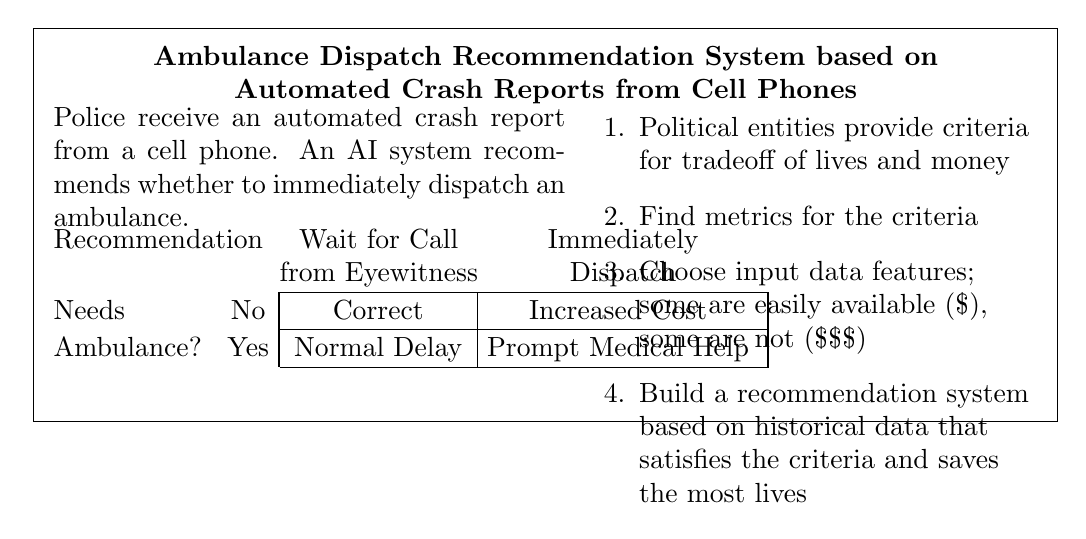
\begin{tikzpicture}[x=10mm, y=10mm, node distance = 3mm]
%	\clip (0,0) rectangle (13,5);
	\draw (0,0) rectangle (13,5);
	\node (Title) at (6.5,4.4) [align=center] { \bf Ambulance Dispatch Recommendation System based on \\  \bf Automated Crash Reports from Cell Phones};
	\node (A) at (3.5,3.2) [] {
		\begin{tabular}{p{6.5cm}}
			Police receive an automated crash report from a cell phone.  
			An AI system recommends whether to immediately dispatch an ambulance.
			%Should they immediately dispatch an ambulance?
		\end{tabular}
	};
	\node [below= 1.6cm of A.west, anchor=west] (D) {
		\begin{tabular}{l @{} c @{\hspace{2pt}} | @{} c @{} | @{} c @{} |}
		\multicolumn{2}{l}{Recommendation} & \multicolumn{1}{ @{} c @{} }{Wait for Call} & \multicolumn{1}{ @{} c @{} }{Immediately} \cr
		&\multicolumn{1}{ @{} c @{} }{} & \multicolumn{1}{ @{} c @{} }{from Eyewitness} & \multicolumn{1}{ @{} c @{} }{Dispatch} \cr\cline{3-4}
		Needs & No & Correct & Increased Cost
			\vrule width 0pt height 10pt depth 2pt \cr\cline{3-4}
		Ambulance? \ \ &Yes & 
			Normal Delay & \ Prompt Medical Help \
			\vrule width 0pt height 10pt depth 2pt \cr\cline{3-4}
		\end{tabular}
	};

	\node (E) [right = -4mm of A.north east, anchor = north west, text width = 6cm] {
		\vspace{-\topsep}
		\begin{enumerate}
			\item Political entities provide criteria for tradeoff of lives and money
			\item Find metrics for the criteria 
			\item Choose input data features; some are easily available (\$), some are not (\$\$\$)
			\item Build a recommendation system based on historical data that satisfies the criteria and saves the most lives
		\end{enumerate}
	};


\end{tikzpicture}
}


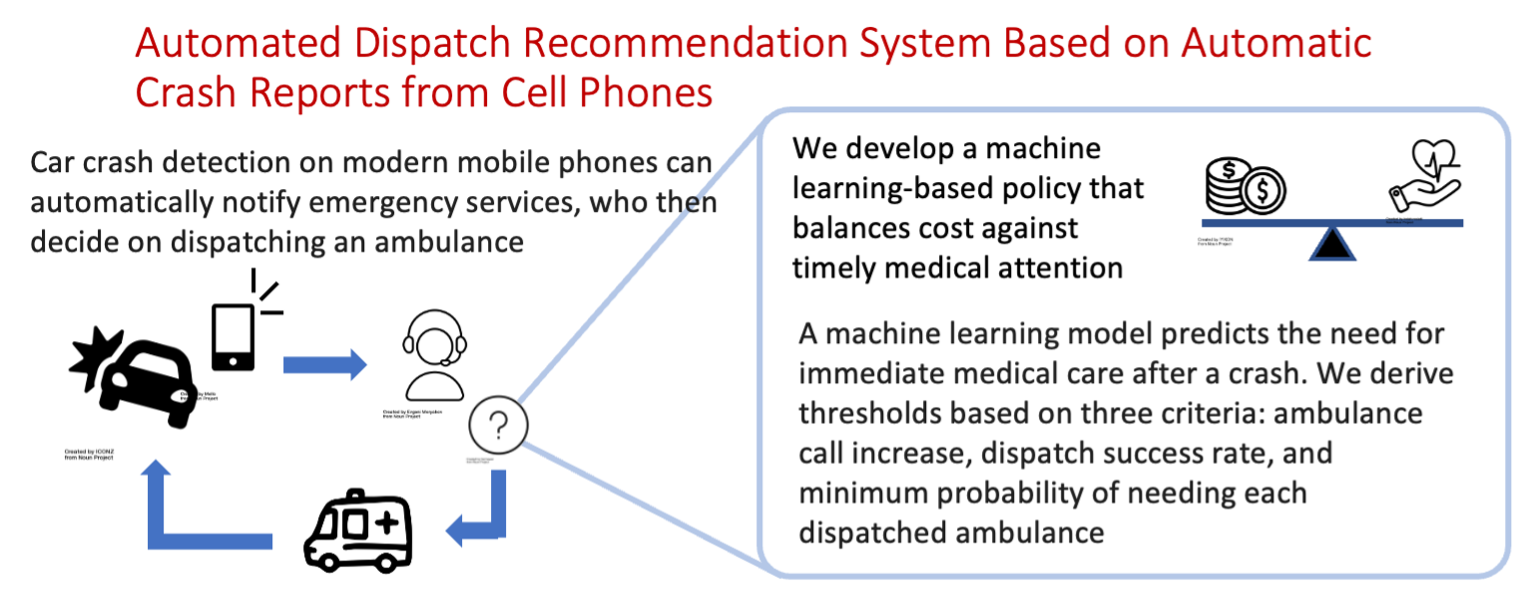
\includegraphics{Graphical_Abstract.png}

\end{graphicalabstract}

% Research highlights
\begin{highlights}
	\item  Supports transferability and benchmarking of different approaches on a public large-scale dataset.  We have made public (on GitHub) the code we used to perform the analysis on data from the Crash Report Sampling System (CRSS) and all of the output data.  
	\item Novel Application motivated by Emerging Technology:  Machine learning classification models for dispatching ambulances based on automated crash reports from cell phones.  
	\item New Use of Dataset:  We used the Crash Report Sampling System (CRSS), which has imputed missing values for some features, but not for all of the features we wanted to use.  For the first time we have seen, we used the software the CRSS authors use for multiple imputation (IVEware) to impute missing values in more features, then compared the results with other imputation methods.
	\item Explicit Incorporation of Imbalanced Costs:  False Positives give additional cost, False Negatives give delayed medical care.
	\item Explicit Incorporation of Political Dimensions: Framing the decision threshold as a government budget question.
	\item Consideration of Marginal Effects of Threshold Shifting
	\item Perennial Machine Learning Challenge:  Imbalanced Datasets
\end{highlights}

% Keywords
% Each keyword is seperated by \sep
\begin{keywords}
 \sep Automated crash notification 
 \sep Ambulance dispatch 
 \sep Emergency medical services  
 \sep Machine learning 
 \sep Imbalanced Cost 
 \sep Imbalanced Data 
 \sep Imputation
\end{keywords}

\maketitle

% Main text

%%%%%
%
% To Do
%
%
%%%%%

%\tableofcontents
%\listoffigures
%\listoftables

%%%%% Introduction
% Introduction
\section{Introduction}
\label{intro}

%%%
\subsection{Scenario}
\label{intro_scenario}

In the (fictitious) city of Springfield, the city council and mayor are debating whether to immediately dispatch ambulances based on automated notifications from cell phones.  Many residents have cell phones (iPhones and Google Pixels) whose accelerometers will detect the deceleration profile of a crash and automatically notify the emergency call center, which immediately dispatches a police officer.  The city leaders are pleased that, because of the automated notifications, the police response to the crash scene is faster.  Should they also immediately dispatch an ambulance, making the medical response faster?

Traditionally, the emergency call center did not know about a crash until an eyewitness called, and the eyewitness could say whether the crash persons needed an ambulance, but that information does not come with an automated crash notification from a cell phone. The notification will come with a location, the emergency dispatcher already has some information (time of day, day of week, weather, urbanicity), and the cell service provider may provide some information about the primary user of the cell phone (age, sex).  With that information, the emergency dispatcher has three options.

\begin{description}
	\item [Always] immediately dispatch an ambulance, most of which will not be needed
	\item [Never] immediately dispatch an ambulance; instead, wait for a call from an eyewitness.  Many of the ambulances eventually sent to crashes had a cell phone notification and could have been sent sooner.  
	\item [Sometimes]  Develop and implement an AI recommendation system to decide which to send immediately, reserving the option to send an ambulance later based on information from an eyewitness.  
\end{description}


In Springfield today, without immediate ambulance dispatch based on automated crash notifications from cell phones, 50\% of dispatched ambulances go to automobile crashes and 10\% of crash persons need an ambulance.  Twenty percent of the crashes first have an automated notification from a cell phone before a call from an eyewitness telling whether or not the crash person needs an ambulance.  The other 80\% of crashes only have an eyewitness call.  Of the crashes with automated notifications from cell phones, 15\% will need an ambulance, 
%($\text{P} = \text{FN} + \text{TP}$), 
and 85\% will not. 
%($\text{N} = \text{TN} + \text{FP}$).  
In Figure \ref{intro_springfield_before} we have scaled the numbers per 100 ambulances sent before implementation of immediate ambulance dispatch.  

[We chose these numbers for clarity of illustration; an actual implementation would use local data.  For details on the 85/15 split, see \S\ref{dataset} Dataset and \S\ref{simplifying_assumptions} Simplifying Assumptions.]

\begin{figure}[h]
	% Image 15 cm wide
% Add 0.5cm on right for margin
\noindent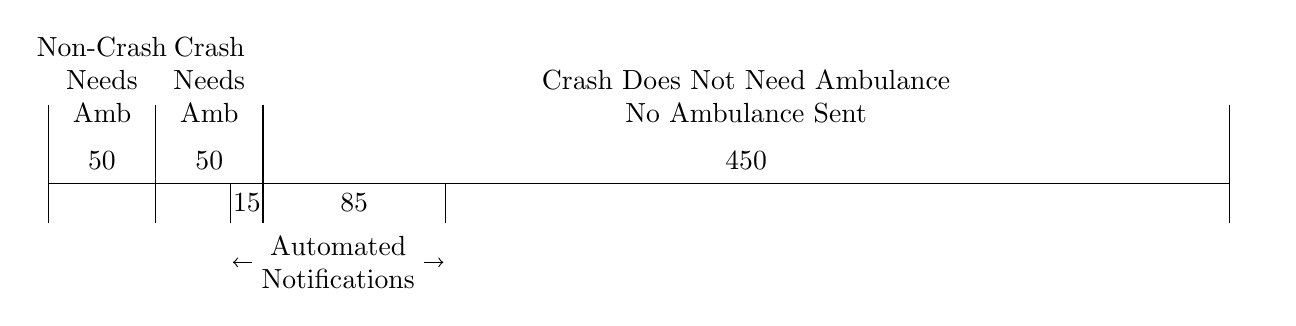
\begin{tikzpicture}[x=0.02727cm, y=0.5cm, font=\normalfont\normalsize]
	\path (568,0) circle (0pt); % Add 0.5 cm on right for margin
	\draw [color=black] (0,0) -- (550,0);
	\draw [color=black] (0,2) -- (0,-1);
	\draw [color=black] (50,2) -- (50,-1);
	\draw [color=black] (100,2) -- (100,-1);
	\draw [color=black] (550,2) -- (550,-1);
	\node (A) at (25,0) {};
	\node (B) [above=-2pt of A, align=center, text=black] {
		Non-Crash \\ Needs \\ Amb \\[0.5em] 50
	};
	\node (C) at (75,0) {};
	\node (D) [above=-2pt of C, align=center, text=black] {
		Crash \\ Needs \\ Amb \\[0.5em] 50
	};
	\node (E) at (325,0) {};
	\node (F) [above=-2pt of E, align=center, text=black] {
		Crash Does Not Need Ambulance \\ No Ambulance Sent \\[0.5em]  450
	};
	\draw [color=black] (85,0) -- (85,-1);
	\draw [color=black] (185,0) -- (185,-1);
	\path (85,0) -- (100,0) node [below, midway, color=black] {
		15
		};
	\path (100,0) -- (185,0) node [below, midway, color=black] {
		85
	};
	
	\draw [<->, color=black]  (86,-2) -- (184,-2) 
		node [midway, color=black, fill=white, align=center] 
		{Automated \\ Notifications};
%	
%	\path (85,-1) -- (185,-1) node 
%		[below, midway, color=black, align=center] {
%		Automated \\ Notifications
%	};
\end{tikzpicture}

\caption{\normalfont\normalsize Springfield before implementing immediate dispatch of ambulances.  Figure accompanies \S\ref{intro_scenario}}
\label{intro_springfield_before}
\end{figure}

\FloatBarrier

If Springfield were to implement an AI recommendation system to immediately dispatch ambulances based on automated calls from cell phones, the recommendations would not perfectly predict which crash persons need an ambulance.    See Figure \ref{intro_springfield_after}, where we have zoomed in on the left side of Figure \ref{intro_springfield_before}. In our per-100-ambulances-currently-sent proportions, the recommendation system would classify each of the automated notifications as needing or not needing an ambulance.  

Of the fifteen automated crash notifications that need an ambulance, the system would correctly classify some of them as needing an ambulance (True Positive, TP), and those crash persons would get medical attention more promptly, which is the goal and benefit of the recommendation system.  The rest of those fifteen would be incorrectly classified as probably not needing an ambulance with a recommendation to wait for a call from an eyewitness before sending one (False Negative, FN).  Note that the false negatives get an ambulance just as quickly under the new system as under the old,  with an ambulance dispatched upon call from an eyewitness.  

Of the 85 automated notifications that do not need an ambulance, some would be correctly classified (True Negative, TN), but some would be incorrectly classified and we would immediately dispatch an unneeded ambulance (False Positive, FP).  Besides the cost of administration, those additional ambulance runs are the cost of immediately dispatching ambulances.  In the short term those additional ambulance runs could be more than current resources (ambulances and their teams) could handle, and in the long term could be unnacceptably expensive.  

\begin{figure}[h]
	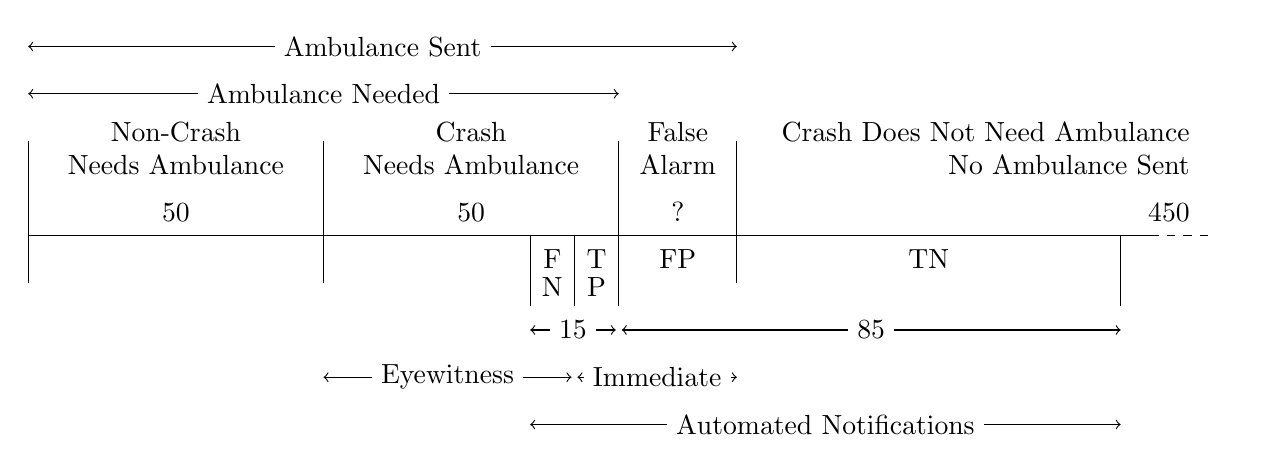
\begin{tikzpicture}[x=0.075cm, y=0.6cm, font=\normalfont\normalsize] % 15 cm wide
	\path (207,0) circle (0pt);
	\draw [color=black] (0,0) -- (190,0);
	\draw [color=black, dashed] (190,0) -- (200,0);
	\draw [color=black] (0,2) -- (0,-1);
	\draw [color=black] (50,2) -- (50,-1);
	\draw [color=black] (100,2) -- (100,-1.5);
	\draw [color=black] (120,2) -- (120,-1);
	\node (A) at (25,0) {};
	\node (B) [above=-2pt of A, align=center, text=black] {
		Non-Crash \\ Needs Ambulance \\[0.5em] 50
	};
	\node (C) at (75,0) {};
	\node (D) [above=-2pt of C, align=center, text=black] {
		Crash \\ Needs Ambulance \\[0.5em] 50
	};
	\node (E) at (200,0) {};
	\node (F) [above left =-2pt and 0pt of E, align=right, text=black] {
		Crash Does Not Need Ambulance \\ No Ambulance Sent \\[0.5em] 450
	};
	\node (G) at (110,0) {};
	\node (H) [above=-2pt of G, align=center, text=black] {
		False \\ Alarm \\[0.5em] ?
	};

	\draw [color=black] (85,0) -- (85,-1.5);
	\draw [color=black] (185,0) -- (185,-1.5);
%	\path (85,-2) -- (100,-2) node [below, midway, color=black] {15};
%	\path (100,-1) -- (185,-1) node [below, midway, color=black] {85};
	
	\draw [<->, color=black]  (100.5,-2) -- (185,-2) 
		node [midway, color=black, fill=white, align=center] 
		{85};

	\draw [<->, color=black]  (85,-2) -- (99.5,-2) 
		node [midway, color=black, fill=white, align=center] 
		{15};

	\draw [<->, color=black]  (50,-3) -- (92,-3) 
		node [midway, color=black, fill=white, align=center] 
		{Eyewitness};

	\draw [<->, color=black]  (93,-3) -- (120,-3) 
		node [midway, color=black, fill=white, align=center] 
		{Immediate};

	\draw [<->, color=black]  (85,-4) -- (185,-4) 
		node [midway, color=black, fill=white, align=center] 
		{Automated Notifications};

	\draw [<->, color=black]  (0,3) -- (100,3) 
		node [midway, color=black, fill=white, align=center] 
		{Ambulance Needed};

	\draw [<->, color=black]  (0,4) -- (120,4) 
		node [midway, color=black, fill=white, align=center] 
		{Ambulance Sent};

%	\node (G) at (110,2) [color=black, align=left] {False \\  Alarm};
	\path (100,-0.5) -- (120,-0.5) node [midway, color=black] {FP};
	\path (120,-0.5) -- (185,-0.5) node [midway, color=black] {TN};
	\draw [color=black] (92.5,0) -- (92.5,-1.5);
	\path (85,-0.5) -- (92.5,-0.5) node [midway, color=black] {F};
	\path (85,-1.2) -- (92.5,-1.0) node [midway, color=black] {N};
	\path (100,-0.5) -- (92.5,-0.5) node [midway, color=black] {T};
	\path (100,-1.2) -- (92.5,-1.0) node [midway, color=black] {P};
\end{tikzpicture}

\caption{\normalfont\normalsize Springfield after implementing immediate dispatch of ambulances.  Figure accompanies \S\ref{intro_scenario}}
\label{intro_springfield_after}
\end{figure}

\FloatBarrier

The leaders of Springfield need to choose a balance between the benefit of more prompt medical attention and the cost of sending more ambulances.  The tradeoff of lives and money is not ethically or morally comfortable, but that is the choice governments make when they set budgets for health care and emergency services.  In the confusion matrices in Figure \ref{intro_confusion}, Springfield would love to increase TP without increasing FP, but the recommendation system will not give perfect predictions.  

\begin{figure}[h]
\begin{minipage}{\linewidth}
{\normalfont\normalsize
\begin{tabular}{p{2in}p{3in}}
\begin{tabular}{c c  | c | c | c}
	& \multicolumn{1}{c}{} & \multicolumn{2}{c}{Prediction}  \cr
	&\multicolumn{1}{c}{} & \multicolumn{1}{c}{PN} & \multicolumn{1}{c}{PP} \cr\cline{3-4}
	\multirow{2}{*}{Actual} & N & TN & FP \vrule width 0pt height 10pt depth 2pt \cr\cline{3-4}
	 & P & FN & TP	\vrule width 0pt height 10pt depth 4pt \cr\cline{3-4}
\end{tabular}
&
\begin{tabular}{c c  | c | c | c}
	\multicolumn{2}{@{}l}{Recommendation} & \multicolumn{1}{ @{} c @{} }{Wait for Call} & \multicolumn{1}{ @{} c @{} }{Immediately}   \cr
	&\multicolumn{1}{ @{} c @{} }{} & \multicolumn{1}{ @{} c @{} }{from Eyewitness} & \multicolumn{1}{ @{} c @{} }{Dispatch} \cr\cline{3-4}
	Needs & No & Correct & Increased Cost
		\vrule width 0pt height 10pt depth 2pt \cr\cline{3-4}
	Ambulance? \ \ &Yes & 
		Normal Delay & \ Prompt Medical Help \
		\vrule width 0pt height 10pt depth 4pt \cr\cline{3-4}
\end{tabular}
\cr		
\end{tabular}
}
\end{minipage}
\caption{\normalfont\normalsize Confusion matrix for ambulance dispatch.  Figure accompanies \S\ref{intro_scenario}}
\label{intro_confusion}
\end{figure}

\FloatBarrier

Building Springfield's AI recommendation system starts with an historical dataset with the features the emergency dispatchers will have at the time of the automated notification, (time of day, weather, maybe age and sex, possibly more information) and whether that historical crash person needed an ambulance (supervised learning).  A machine learning algorithm learns a model of the data, and when an automated crash notification comes in, given the data available, the model returns a value $p \in [0,1]$ that increases with the probability that the crash person needs an ambulance.  The city council and mayor need to choose a decision threshold $\theta$ such that if, for a particular crash notification, $p>\theta$, then immediately dispatch an ambulance; if $p<\theta$, wait for a call from an eyewitness.  Choosing a decision threshold of $p=1$ would mean never immediately dispatching an ambulance, and choosing $p=0$ would be always; the town leaders want to know how to choose a $p$ between the two extremes that fits their values and their budget.

The histogram in Figure \ref{intro_ideal} shows typical model output.  The model generally gives lower $p$ values to crash persons who do not need an ambulance (Neg) and higher $p$ values to crash persons who do need an ambulance (Pos), but there is significant overlap.  The most obvious feature of the histogram is the class imbalance, that there are many more Neg than Pos, in fact $85/15 \approx 6$ Neg for each Pos.  

Given a choice of decision threshold $\theta$, Springfield would immediately dispatch ambulances to all of the crashes with a $p$ value to the right of $\theta$.  The Pos (Needs ambulance) to the right of $\theta$ would get more prompt medical attention (TP), but the Neg (Does not need ambulance) to the right of $\theta$ would be wasted ambulance runs (FP) .  At $\theta = 0.8$, TP and FP are about equal, but as we consider smaller $\theta$ the number of TP increases by smaller and smaller amounts while the number of FP grows dramatically.  

\begin{figure}[h]
\centering
	%% Creator: Matplotlib, PGF backend
%%
%% To include the figure in your LaTeX document, write
%%   \input{<filename>.pgf}
%%
%% Make sure the required packages are loaded in your preamble
%%   \usepackage{pgf}
%%
%% Also ensure that all the required font packages are loaded; for instance,
%% the lmodern package is sometimes necessary when using math font.
%%   \usepackage{lmodern}
%%
%% Figures using additional raster images can only be included by \input if
%% they are in the same directory as the main LaTeX file. For loading figures
%% from other directories you can use the `import` package
%%   \usepackage{import}
%%
%% and then include the figures with
%%   \import{<path to file>}{<filename>.pgf}
%%
%% Matplotlib used the following preamble
%%   
%%   \usepackage{fontspec}
%%   \makeatletter\@ifpackageloaded{underscore}{}{\usepackage[strings]{underscore}}\makeatother
%%
\begingroup%
\makeatletter%
\begin{pgfpicture}%
\pgfpathrectangle{\pgfpointorigin}{\pgfqpoint{4.084250in}{1.703778in}}%
\pgfusepath{use as bounding box, clip}%
\begin{pgfscope}%
\pgfsetbuttcap%
\pgfsetmiterjoin%
\definecolor{currentfill}{rgb}{1.000000,1.000000,1.000000}%
\pgfsetfillcolor{currentfill}%
\pgfsetlinewidth{0.000000pt}%
\definecolor{currentstroke}{rgb}{1.000000,1.000000,1.000000}%
\pgfsetstrokecolor{currentstroke}%
\pgfsetdash{}{0pt}%
\pgfpathmoveto{\pgfqpoint{0.000000in}{0.000000in}}%
\pgfpathlineto{\pgfqpoint{4.084250in}{0.000000in}}%
\pgfpathlineto{\pgfqpoint{4.084250in}{1.703777in}}%
\pgfpathlineto{\pgfqpoint{0.000000in}{1.703777in}}%
\pgfpathlineto{\pgfqpoint{0.000000in}{0.000000in}}%
\pgfpathclose%
\pgfusepath{fill}%
\end{pgfscope}%
\begin{pgfscope}%
\pgfsetbuttcap%
\pgfsetmiterjoin%
\definecolor{currentfill}{rgb}{1.000000,1.000000,1.000000}%
\pgfsetfillcolor{currentfill}%
\pgfsetlinewidth{0.000000pt}%
\definecolor{currentstroke}{rgb}{0.000000,0.000000,0.000000}%
\pgfsetstrokecolor{currentstroke}%
\pgfsetstrokeopacity{0.000000}%
\pgfsetdash{}{0pt}%
\pgfpathmoveto{\pgfqpoint{0.546750in}{0.498777in}}%
\pgfpathlineto{\pgfqpoint{4.034250in}{0.498777in}}%
\pgfpathlineto{\pgfqpoint{4.034250in}{1.653777in}}%
\pgfpathlineto{\pgfqpoint{0.546750in}{1.653777in}}%
\pgfpathlineto{\pgfqpoint{0.546750in}{0.498777in}}%
\pgfpathclose%
\pgfusepath{fill}%
\end{pgfscope}%
\begin{pgfscope}%
\pgfpathrectangle{\pgfqpoint{0.546750in}{0.498777in}}{\pgfqpoint{3.487500in}{1.155000in}}%
\pgfusepath{clip}%
\pgfsetbuttcap%
\pgfsetmiterjoin%
\pgfsetlinewidth{1.003750pt}%
\definecolor{currentstroke}{rgb}{0.000000,0.000000,0.000000}%
\pgfsetstrokecolor{currentstroke}%
\pgfsetdash{}{0pt}%
\pgfpathmoveto{\pgfqpoint{0.641863in}{0.498777in}}%
\pgfpathlineto{\pgfqpoint{0.705273in}{0.498777in}}%
\pgfpathlineto{\pgfqpoint{0.705273in}{0.498777in}}%
\pgfpathlineto{\pgfqpoint{0.641863in}{0.498777in}}%
\pgfpathlineto{\pgfqpoint{0.641863in}{0.498777in}}%
\pgfpathclose%
\pgfusepath{stroke}%
\end{pgfscope}%
\begin{pgfscope}%
\pgfpathrectangle{\pgfqpoint{0.546750in}{0.498777in}}{\pgfqpoint{3.487500in}{1.155000in}}%
\pgfusepath{clip}%
\pgfsetbuttcap%
\pgfsetmiterjoin%
\pgfsetlinewidth{1.003750pt}%
\definecolor{currentstroke}{rgb}{0.000000,0.000000,0.000000}%
\pgfsetstrokecolor{currentstroke}%
\pgfsetdash{}{0pt}%
\pgfpathmoveto{\pgfqpoint{0.800386in}{0.498777in}}%
\pgfpathlineto{\pgfqpoint{0.863795in}{0.498777in}}%
\pgfpathlineto{\pgfqpoint{0.863795in}{0.529695in}}%
\pgfpathlineto{\pgfqpoint{0.800386in}{0.529695in}}%
\pgfpathlineto{\pgfqpoint{0.800386in}{0.498777in}}%
\pgfpathclose%
\pgfusepath{stroke}%
\end{pgfscope}%
\begin{pgfscope}%
\pgfpathrectangle{\pgfqpoint{0.546750in}{0.498777in}}{\pgfqpoint{3.487500in}{1.155000in}}%
\pgfusepath{clip}%
\pgfsetbuttcap%
\pgfsetmiterjoin%
\pgfsetlinewidth{1.003750pt}%
\definecolor{currentstroke}{rgb}{0.000000,0.000000,0.000000}%
\pgfsetstrokecolor{currentstroke}%
\pgfsetdash{}{0pt}%
\pgfpathmoveto{\pgfqpoint{0.958909in}{0.498777in}}%
\pgfpathlineto{\pgfqpoint{1.022318in}{0.498777in}}%
\pgfpathlineto{\pgfqpoint{1.022318in}{0.736639in}}%
\pgfpathlineto{\pgfqpoint{0.958909in}{0.736639in}}%
\pgfpathlineto{\pgfqpoint{0.958909in}{0.498777in}}%
\pgfpathclose%
\pgfusepath{stroke}%
\end{pgfscope}%
\begin{pgfscope}%
\pgfpathrectangle{\pgfqpoint{0.546750in}{0.498777in}}{\pgfqpoint{3.487500in}{1.155000in}}%
\pgfusepath{clip}%
\pgfsetbuttcap%
\pgfsetmiterjoin%
\pgfsetlinewidth{1.003750pt}%
\definecolor{currentstroke}{rgb}{0.000000,0.000000,0.000000}%
\pgfsetstrokecolor{currentstroke}%
\pgfsetdash{}{0pt}%
\pgfpathmoveto{\pgfqpoint{1.117432in}{0.498777in}}%
\pgfpathlineto{\pgfqpoint{1.180841in}{0.498777in}}%
\pgfpathlineto{\pgfqpoint{1.180841in}{1.084597in}}%
\pgfpathlineto{\pgfqpoint{1.117432in}{1.084597in}}%
\pgfpathlineto{\pgfqpoint{1.117432in}{0.498777in}}%
\pgfpathclose%
\pgfusepath{stroke}%
\end{pgfscope}%
\begin{pgfscope}%
\pgfpathrectangle{\pgfqpoint{0.546750in}{0.498777in}}{\pgfqpoint{3.487500in}{1.155000in}}%
\pgfusepath{clip}%
\pgfsetbuttcap%
\pgfsetmiterjoin%
\pgfsetlinewidth{1.003750pt}%
\definecolor{currentstroke}{rgb}{0.000000,0.000000,0.000000}%
\pgfsetstrokecolor{currentstroke}%
\pgfsetdash{}{0pt}%
\pgfpathmoveto{\pgfqpoint{1.275954in}{0.498777in}}%
\pgfpathlineto{\pgfqpoint{1.339363in}{0.498777in}}%
\pgfpathlineto{\pgfqpoint{1.339363in}{1.395604in}}%
\pgfpathlineto{\pgfqpoint{1.275954in}{1.395604in}}%
\pgfpathlineto{\pgfqpoint{1.275954in}{0.498777in}}%
\pgfpathclose%
\pgfusepath{stroke}%
\end{pgfscope}%
\begin{pgfscope}%
\pgfpathrectangle{\pgfqpoint{0.546750in}{0.498777in}}{\pgfqpoint{3.487500in}{1.155000in}}%
\pgfusepath{clip}%
\pgfsetbuttcap%
\pgfsetmiterjoin%
\pgfsetlinewidth{1.003750pt}%
\definecolor{currentstroke}{rgb}{0.000000,0.000000,0.000000}%
\pgfsetstrokecolor{currentstroke}%
\pgfsetdash{}{0pt}%
\pgfpathmoveto{\pgfqpoint{1.434477in}{0.498777in}}%
\pgfpathlineto{\pgfqpoint{1.497886in}{0.498777in}}%
\pgfpathlineto{\pgfqpoint{1.497886in}{1.566783in}}%
\pgfpathlineto{\pgfqpoint{1.434477in}{1.566783in}}%
\pgfpathlineto{\pgfqpoint{1.434477in}{0.498777in}}%
\pgfpathclose%
\pgfusepath{stroke}%
\end{pgfscope}%
\begin{pgfscope}%
\pgfpathrectangle{\pgfqpoint{0.546750in}{0.498777in}}{\pgfqpoint{3.487500in}{1.155000in}}%
\pgfusepath{clip}%
\pgfsetbuttcap%
\pgfsetmiterjoin%
\pgfsetlinewidth{1.003750pt}%
\definecolor{currentstroke}{rgb}{0.000000,0.000000,0.000000}%
\pgfsetstrokecolor{currentstroke}%
\pgfsetdash{}{0pt}%
\pgfpathmoveto{\pgfqpoint{1.593000in}{0.498777in}}%
\pgfpathlineto{\pgfqpoint{1.656409in}{0.498777in}}%
\pgfpathlineto{\pgfqpoint{1.656409in}{1.598777in}}%
\pgfpathlineto{\pgfqpoint{1.593000in}{1.598777in}}%
\pgfpathlineto{\pgfqpoint{1.593000in}{0.498777in}}%
\pgfpathclose%
\pgfusepath{stroke}%
\end{pgfscope}%
\begin{pgfscope}%
\pgfpathrectangle{\pgfqpoint{0.546750in}{0.498777in}}{\pgfqpoint{3.487500in}{1.155000in}}%
\pgfusepath{clip}%
\pgfsetbuttcap%
\pgfsetmiterjoin%
\pgfsetlinewidth{1.003750pt}%
\definecolor{currentstroke}{rgb}{0.000000,0.000000,0.000000}%
\pgfsetstrokecolor{currentstroke}%
\pgfsetdash{}{0pt}%
\pgfpathmoveto{\pgfqpoint{1.751523in}{0.498777in}}%
\pgfpathlineto{\pgfqpoint{1.814932in}{0.498777in}}%
\pgfpathlineto{\pgfqpoint{1.814932in}{1.545776in}}%
\pgfpathlineto{\pgfqpoint{1.751523in}{1.545776in}}%
\pgfpathlineto{\pgfqpoint{1.751523in}{0.498777in}}%
\pgfpathclose%
\pgfusepath{stroke}%
\end{pgfscope}%
\begin{pgfscope}%
\pgfpathrectangle{\pgfqpoint{0.546750in}{0.498777in}}{\pgfqpoint{3.487500in}{1.155000in}}%
\pgfusepath{clip}%
\pgfsetbuttcap%
\pgfsetmiterjoin%
\pgfsetlinewidth{1.003750pt}%
\definecolor{currentstroke}{rgb}{0.000000,0.000000,0.000000}%
\pgfsetstrokecolor{currentstroke}%
\pgfsetdash{}{0pt}%
\pgfpathmoveto{\pgfqpoint{1.910045in}{0.498777in}}%
\pgfpathlineto{\pgfqpoint{1.973454in}{0.498777in}}%
\pgfpathlineto{\pgfqpoint{1.973454in}{1.432447in}}%
\pgfpathlineto{\pgfqpoint{1.910045in}{1.432447in}}%
\pgfpathlineto{\pgfqpoint{1.910045in}{0.498777in}}%
\pgfpathclose%
\pgfusepath{stroke}%
\end{pgfscope}%
\begin{pgfscope}%
\pgfpathrectangle{\pgfqpoint{0.546750in}{0.498777in}}{\pgfqpoint{3.487500in}{1.155000in}}%
\pgfusepath{clip}%
\pgfsetbuttcap%
\pgfsetmiterjoin%
\pgfsetlinewidth{1.003750pt}%
\definecolor{currentstroke}{rgb}{0.000000,0.000000,0.000000}%
\pgfsetstrokecolor{currentstroke}%
\pgfsetdash{}{0pt}%
\pgfpathmoveto{\pgfqpoint{2.068568in}{0.498777in}}%
\pgfpathlineto{\pgfqpoint{2.131977in}{0.498777in}}%
\pgfpathlineto{\pgfqpoint{2.131977in}{1.290140in}}%
\pgfpathlineto{\pgfqpoint{2.068568in}{1.290140in}}%
\pgfpathlineto{\pgfqpoint{2.068568in}{0.498777in}}%
\pgfpathclose%
\pgfusepath{stroke}%
\end{pgfscope}%
\begin{pgfscope}%
\pgfpathrectangle{\pgfqpoint{0.546750in}{0.498777in}}{\pgfqpoint{3.487500in}{1.155000in}}%
\pgfusepath{clip}%
\pgfsetbuttcap%
\pgfsetmiterjoin%
\pgfsetlinewidth{1.003750pt}%
\definecolor{currentstroke}{rgb}{0.000000,0.000000,0.000000}%
\pgfsetstrokecolor{currentstroke}%
\pgfsetdash{}{0pt}%
\pgfpathmoveto{\pgfqpoint{2.227091in}{0.498777in}}%
\pgfpathlineto{\pgfqpoint{2.290500in}{0.498777in}}%
\pgfpathlineto{\pgfqpoint{2.290500in}{1.122624in}}%
\pgfpathlineto{\pgfqpoint{2.227091in}{1.122624in}}%
\pgfpathlineto{\pgfqpoint{2.227091in}{0.498777in}}%
\pgfpathclose%
\pgfusepath{stroke}%
\end{pgfscope}%
\begin{pgfscope}%
\pgfpathrectangle{\pgfqpoint{0.546750in}{0.498777in}}{\pgfqpoint{3.487500in}{1.155000in}}%
\pgfusepath{clip}%
\pgfsetbuttcap%
\pgfsetmiterjoin%
\pgfsetlinewidth{1.003750pt}%
\definecolor{currentstroke}{rgb}{0.000000,0.000000,0.000000}%
\pgfsetstrokecolor{currentstroke}%
\pgfsetdash{}{0pt}%
\pgfpathmoveto{\pgfqpoint{2.385613in}{0.498777in}}%
\pgfpathlineto{\pgfqpoint{2.449023in}{0.498777in}}%
\pgfpathlineto{\pgfqpoint{2.449023in}{0.989797in}}%
\pgfpathlineto{\pgfqpoint{2.385613in}{0.989797in}}%
\pgfpathlineto{\pgfqpoint{2.385613in}{0.498777in}}%
\pgfpathclose%
\pgfusepath{stroke}%
\end{pgfscope}%
\begin{pgfscope}%
\pgfpathrectangle{\pgfqpoint{0.546750in}{0.498777in}}{\pgfqpoint{3.487500in}{1.155000in}}%
\pgfusepath{clip}%
\pgfsetbuttcap%
\pgfsetmiterjoin%
\pgfsetlinewidth{1.003750pt}%
\definecolor{currentstroke}{rgb}{0.000000,0.000000,0.000000}%
\pgfsetstrokecolor{currentstroke}%
\pgfsetdash{}{0pt}%
\pgfpathmoveto{\pgfqpoint{2.544136in}{0.498777in}}%
\pgfpathlineto{\pgfqpoint{2.607545in}{0.498777in}}%
\pgfpathlineto{\pgfqpoint{2.607545in}{0.870328in}}%
\pgfpathlineto{\pgfqpoint{2.544136in}{0.870328in}}%
\pgfpathlineto{\pgfqpoint{2.544136in}{0.498777in}}%
\pgfpathclose%
\pgfusepath{stroke}%
\end{pgfscope}%
\begin{pgfscope}%
\pgfpathrectangle{\pgfqpoint{0.546750in}{0.498777in}}{\pgfqpoint{3.487500in}{1.155000in}}%
\pgfusepath{clip}%
\pgfsetbuttcap%
\pgfsetmiterjoin%
\pgfsetlinewidth{1.003750pt}%
\definecolor{currentstroke}{rgb}{0.000000,0.000000,0.000000}%
\pgfsetstrokecolor{currentstroke}%
\pgfsetdash{}{0pt}%
\pgfpathmoveto{\pgfqpoint{2.702659in}{0.498777in}}%
\pgfpathlineto{\pgfqpoint{2.766068in}{0.498777in}}%
\pgfpathlineto{\pgfqpoint{2.766068in}{0.856646in}}%
\pgfpathlineto{\pgfqpoint{2.702659in}{0.856646in}}%
\pgfpathlineto{\pgfqpoint{2.702659in}{0.498777in}}%
\pgfpathclose%
\pgfusepath{stroke}%
\end{pgfscope}%
\begin{pgfscope}%
\pgfpathrectangle{\pgfqpoint{0.546750in}{0.498777in}}{\pgfqpoint{3.487500in}{1.155000in}}%
\pgfusepath{clip}%
\pgfsetbuttcap%
\pgfsetmiterjoin%
\pgfsetlinewidth{1.003750pt}%
\definecolor{currentstroke}{rgb}{0.000000,0.000000,0.000000}%
\pgfsetstrokecolor{currentstroke}%
\pgfsetdash{}{0pt}%
\pgfpathmoveto{\pgfqpoint{2.861182in}{0.498777in}}%
\pgfpathlineto{\pgfqpoint{2.924591in}{0.498777in}}%
\pgfpathlineto{\pgfqpoint{2.924591in}{0.700766in}}%
\pgfpathlineto{\pgfqpoint{2.861182in}{0.700766in}}%
\pgfpathlineto{\pgfqpoint{2.861182in}{0.498777in}}%
\pgfpathclose%
\pgfusepath{stroke}%
\end{pgfscope}%
\begin{pgfscope}%
\pgfpathrectangle{\pgfqpoint{0.546750in}{0.498777in}}{\pgfqpoint{3.487500in}{1.155000in}}%
\pgfusepath{clip}%
\pgfsetbuttcap%
\pgfsetmiterjoin%
\pgfsetlinewidth{1.003750pt}%
\definecolor{currentstroke}{rgb}{0.000000,0.000000,0.000000}%
\pgfsetstrokecolor{currentstroke}%
\pgfsetdash{}{0pt}%
\pgfpathmoveto{\pgfqpoint{3.019704in}{0.498777in}}%
\pgfpathlineto{\pgfqpoint{3.083113in}{0.498777in}}%
\pgfpathlineto{\pgfqpoint{3.083113in}{0.650134in}}%
\pgfpathlineto{\pgfqpoint{3.019704in}{0.650134in}}%
\pgfpathlineto{\pgfqpoint{3.019704in}{0.498777in}}%
\pgfpathclose%
\pgfusepath{stroke}%
\end{pgfscope}%
\begin{pgfscope}%
\pgfpathrectangle{\pgfqpoint{0.546750in}{0.498777in}}{\pgfqpoint{3.487500in}{1.155000in}}%
\pgfusepath{clip}%
\pgfsetbuttcap%
\pgfsetmiterjoin%
\pgfsetlinewidth{1.003750pt}%
\definecolor{currentstroke}{rgb}{0.000000,0.000000,0.000000}%
\pgfsetstrokecolor{currentstroke}%
\pgfsetdash{}{0pt}%
\pgfpathmoveto{\pgfqpoint{3.178227in}{0.498777in}}%
\pgfpathlineto{\pgfqpoint{3.241636in}{0.498777in}}%
\pgfpathlineto{\pgfqpoint{3.241636in}{0.603380in}}%
\pgfpathlineto{\pgfqpoint{3.178227in}{0.603380in}}%
\pgfpathlineto{\pgfqpoint{3.178227in}{0.498777in}}%
\pgfpathclose%
\pgfusepath{stroke}%
\end{pgfscope}%
\begin{pgfscope}%
\pgfpathrectangle{\pgfqpoint{0.546750in}{0.498777in}}{\pgfqpoint{3.487500in}{1.155000in}}%
\pgfusepath{clip}%
\pgfsetbuttcap%
\pgfsetmiterjoin%
\pgfsetlinewidth{1.003750pt}%
\definecolor{currentstroke}{rgb}{0.000000,0.000000,0.000000}%
\pgfsetstrokecolor{currentstroke}%
\pgfsetdash{}{0pt}%
\pgfpathmoveto{\pgfqpoint{3.336750in}{0.498777in}}%
\pgfpathlineto{\pgfqpoint{3.400159in}{0.498777in}}%
\pgfpathlineto{\pgfqpoint{3.400159in}{0.574294in}}%
\pgfpathlineto{\pgfqpoint{3.336750in}{0.574294in}}%
\pgfpathlineto{\pgfqpoint{3.336750in}{0.498777in}}%
\pgfpathclose%
\pgfusepath{stroke}%
\end{pgfscope}%
\begin{pgfscope}%
\pgfpathrectangle{\pgfqpoint{0.546750in}{0.498777in}}{\pgfqpoint{3.487500in}{1.155000in}}%
\pgfusepath{clip}%
\pgfsetbuttcap%
\pgfsetmiterjoin%
\pgfsetlinewidth{1.003750pt}%
\definecolor{currentstroke}{rgb}{0.000000,0.000000,0.000000}%
\pgfsetstrokecolor{currentstroke}%
\pgfsetdash{}{0pt}%
\pgfpathmoveto{\pgfqpoint{3.495273in}{0.498777in}}%
\pgfpathlineto{\pgfqpoint{3.558682in}{0.498777in}}%
\pgfpathlineto{\pgfqpoint{3.558682in}{0.550486in}}%
\pgfpathlineto{\pgfqpoint{3.495273in}{0.550486in}}%
\pgfpathlineto{\pgfqpoint{3.495273in}{0.498777in}}%
\pgfpathclose%
\pgfusepath{stroke}%
\end{pgfscope}%
\begin{pgfscope}%
\pgfpathrectangle{\pgfqpoint{0.546750in}{0.498777in}}{\pgfqpoint{3.487500in}{1.155000in}}%
\pgfusepath{clip}%
\pgfsetbuttcap%
\pgfsetmiterjoin%
\pgfsetlinewidth{1.003750pt}%
\definecolor{currentstroke}{rgb}{0.000000,0.000000,0.000000}%
\pgfsetstrokecolor{currentstroke}%
\pgfsetdash{}{0pt}%
\pgfpathmoveto{\pgfqpoint{3.653795in}{0.498777in}}%
\pgfpathlineto{\pgfqpoint{3.717204in}{0.498777in}}%
\pgfpathlineto{\pgfqpoint{3.717204in}{0.534651in}}%
\pgfpathlineto{\pgfqpoint{3.653795in}{0.534651in}}%
\pgfpathlineto{\pgfqpoint{3.653795in}{0.498777in}}%
\pgfpathclose%
\pgfusepath{stroke}%
\end{pgfscope}%
\begin{pgfscope}%
\pgfpathrectangle{\pgfqpoint{0.546750in}{0.498777in}}{\pgfqpoint{3.487500in}{1.155000in}}%
\pgfusepath{clip}%
\pgfsetbuttcap%
\pgfsetmiterjoin%
\pgfsetlinewidth{1.003750pt}%
\definecolor{currentstroke}{rgb}{0.000000,0.000000,0.000000}%
\pgfsetstrokecolor{currentstroke}%
\pgfsetdash{}{0pt}%
\pgfpathmoveto{\pgfqpoint{3.812318in}{0.498777in}}%
\pgfpathlineto{\pgfqpoint{3.875727in}{0.498777in}}%
\pgfpathlineto{\pgfqpoint{3.875727in}{0.498777in}}%
\pgfpathlineto{\pgfqpoint{3.812318in}{0.498777in}}%
\pgfpathlineto{\pgfqpoint{3.812318in}{0.498777in}}%
\pgfpathclose%
\pgfusepath{stroke}%
\end{pgfscope}%
\begin{pgfscope}%
\pgfpathrectangle{\pgfqpoint{0.546750in}{0.498777in}}{\pgfqpoint{3.487500in}{1.155000in}}%
\pgfusepath{clip}%
\pgfsetbuttcap%
\pgfsetmiterjoin%
\definecolor{currentfill}{rgb}{0.000000,0.000000,0.000000}%
\pgfsetfillcolor{currentfill}%
\pgfsetlinewidth{0.000000pt}%
\definecolor{currentstroke}{rgb}{0.000000,0.000000,0.000000}%
\pgfsetstrokecolor{currentstroke}%
\pgfsetstrokeopacity{0.000000}%
\pgfsetdash{}{0pt}%
\pgfpathmoveto{\pgfqpoint{0.705273in}{0.498777in}}%
\pgfpathlineto{\pgfqpoint{0.768682in}{0.498777in}}%
\pgfpathlineto{\pgfqpoint{0.768682in}{0.498777in}}%
\pgfpathlineto{\pgfqpoint{0.705273in}{0.498777in}}%
\pgfpathlineto{\pgfqpoint{0.705273in}{0.498777in}}%
\pgfpathclose%
\pgfusepath{fill}%
\end{pgfscope}%
\begin{pgfscope}%
\pgfpathrectangle{\pgfqpoint{0.546750in}{0.498777in}}{\pgfqpoint{3.487500in}{1.155000in}}%
\pgfusepath{clip}%
\pgfsetbuttcap%
\pgfsetmiterjoin%
\definecolor{currentfill}{rgb}{0.000000,0.000000,0.000000}%
\pgfsetfillcolor{currentfill}%
\pgfsetlinewidth{0.000000pt}%
\definecolor{currentstroke}{rgb}{0.000000,0.000000,0.000000}%
\pgfsetstrokecolor{currentstroke}%
\pgfsetstrokeopacity{0.000000}%
\pgfsetdash{}{0pt}%
\pgfpathmoveto{\pgfqpoint{0.863795in}{0.498777in}}%
\pgfpathlineto{\pgfqpoint{0.927204in}{0.498777in}}%
\pgfpathlineto{\pgfqpoint{0.927204in}{0.503841in}}%
\pgfpathlineto{\pgfqpoint{0.863795in}{0.503841in}}%
\pgfpathlineto{\pgfqpoint{0.863795in}{0.498777in}}%
\pgfpathclose%
\pgfusepath{fill}%
\end{pgfscope}%
\begin{pgfscope}%
\pgfpathrectangle{\pgfqpoint{0.546750in}{0.498777in}}{\pgfqpoint{3.487500in}{1.155000in}}%
\pgfusepath{clip}%
\pgfsetbuttcap%
\pgfsetmiterjoin%
\definecolor{currentfill}{rgb}{0.000000,0.000000,0.000000}%
\pgfsetfillcolor{currentfill}%
\pgfsetlinewidth{0.000000pt}%
\definecolor{currentstroke}{rgb}{0.000000,0.000000,0.000000}%
\pgfsetstrokecolor{currentstroke}%
\pgfsetstrokeopacity{0.000000}%
\pgfsetdash{}{0pt}%
\pgfpathmoveto{\pgfqpoint{1.022318in}{0.498777in}}%
\pgfpathlineto{\pgfqpoint{1.085727in}{0.498777in}}%
\pgfpathlineto{\pgfqpoint{1.085727in}{0.505887in}}%
\pgfpathlineto{\pgfqpoint{1.022318in}{0.505887in}}%
\pgfpathlineto{\pgfqpoint{1.022318in}{0.498777in}}%
\pgfpathclose%
\pgfusepath{fill}%
\end{pgfscope}%
\begin{pgfscope}%
\pgfpathrectangle{\pgfqpoint{0.546750in}{0.498777in}}{\pgfqpoint{3.487500in}{1.155000in}}%
\pgfusepath{clip}%
\pgfsetbuttcap%
\pgfsetmiterjoin%
\definecolor{currentfill}{rgb}{0.000000,0.000000,0.000000}%
\pgfsetfillcolor{currentfill}%
\pgfsetlinewidth{0.000000pt}%
\definecolor{currentstroke}{rgb}{0.000000,0.000000,0.000000}%
\pgfsetstrokecolor{currentstroke}%
\pgfsetstrokeopacity{0.000000}%
\pgfsetdash{}{0pt}%
\pgfpathmoveto{\pgfqpoint{1.180841in}{0.498777in}}%
\pgfpathlineto{\pgfqpoint{1.244250in}{0.498777in}}%
\pgfpathlineto{\pgfqpoint{1.244250in}{0.511812in}}%
\pgfpathlineto{\pgfqpoint{1.180841in}{0.511812in}}%
\pgfpathlineto{\pgfqpoint{1.180841in}{0.498777in}}%
\pgfpathclose%
\pgfusepath{fill}%
\end{pgfscope}%
\begin{pgfscope}%
\pgfpathrectangle{\pgfqpoint{0.546750in}{0.498777in}}{\pgfqpoint{3.487500in}{1.155000in}}%
\pgfusepath{clip}%
\pgfsetbuttcap%
\pgfsetmiterjoin%
\definecolor{currentfill}{rgb}{0.000000,0.000000,0.000000}%
\pgfsetfillcolor{currentfill}%
\pgfsetlinewidth{0.000000pt}%
\definecolor{currentstroke}{rgb}{0.000000,0.000000,0.000000}%
\pgfsetstrokecolor{currentstroke}%
\pgfsetstrokeopacity{0.000000}%
\pgfsetdash{}{0pt}%
\pgfpathmoveto{\pgfqpoint{1.339363in}{0.498777in}}%
\pgfpathlineto{\pgfqpoint{1.402773in}{0.498777in}}%
\pgfpathlineto{\pgfqpoint{1.402773in}{0.511812in}}%
\pgfpathlineto{\pgfqpoint{1.339363in}{0.511812in}}%
\pgfpathlineto{\pgfqpoint{1.339363in}{0.498777in}}%
\pgfpathclose%
\pgfusepath{fill}%
\end{pgfscope}%
\begin{pgfscope}%
\pgfpathrectangle{\pgfqpoint{0.546750in}{0.498777in}}{\pgfqpoint{3.487500in}{1.155000in}}%
\pgfusepath{clip}%
\pgfsetbuttcap%
\pgfsetmiterjoin%
\definecolor{currentfill}{rgb}{0.000000,0.000000,0.000000}%
\pgfsetfillcolor{currentfill}%
\pgfsetlinewidth{0.000000pt}%
\definecolor{currentstroke}{rgb}{0.000000,0.000000,0.000000}%
\pgfsetstrokecolor{currentstroke}%
\pgfsetstrokeopacity{0.000000}%
\pgfsetdash{}{0pt}%
\pgfpathmoveto{\pgfqpoint{1.497886in}{0.498777in}}%
\pgfpathlineto{\pgfqpoint{1.561295in}{0.498777in}}%
\pgfpathlineto{\pgfqpoint{1.561295in}{0.520323in}}%
\pgfpathlineto{\pgfqpoint{1.497886in}{0.520323in}}%
\pgfpathlineto{\pgfqpoint{1.497886in}{0.498777in}}%
\pgfpathclose%
\pgfusepath{fill}%
\end{pgfscope}%
\begin{pgfscope}%
\pgfpathrectangle{\pgfqpoint{0.546750in}{0.498777in}}{\pgfqpoint{3.487500in}{1.155000in}}%
\pgfusepath{clip}%
\pgfsetbuttcap%
\pgfsetmiterjoin%
\definecolor{currentfill}{rgb}{0.000000,0.000000,0.000000}%
\pgfsetfillcolor{currentfill}%
\pgfsetlinewidth{0.000000pt}%
\definecolor{currentstroke}{rgb}{0.000000,0.000000,0.000000}%
\pgfsetstrokecolor{currentstroke}%
\pgfsetstrokeopacity{0.000000}%
\pgfsetdash{}{0pt}%
\pgfpathmoveto{\pgfqpoint{1.656409in}{0.498777in}}%
\pgfpathlineto{\pgfqpoint{1.719818in}{0.498777in}}%
\pgfpathlineto{\pgfqpoint{1.719818in}{0.525494in}}%
\pgfpathlineto{\pgfqpoint{1.656409in}{0.525494in}}%
\pgfpathlineto{\pgfqpoint{1.656409in}{0.498777in}}%
\pgfpathclose%
\pgfusepath{fill}%
\end{pgfscope}%
\begin{pgfscope}%
\pgfpathrectangle{\pgfqpoint{0.546750in}{0.498777in}}{\pgfqpoint{3.487500in}{1.155000in}}%
\pgfusepath{clip}%
\pgfsetbuttcap%
\pgfsetmiterjoin%
\definecolor{currentfill}{rgb}{0.000000,0.000000,0.000000}%
\pgfsetfillcolor{currentfill}%
\pgfsetlinewidth{0.000000pt}%
\definecolor{currentstroke}{rgb}{0.000000,0.000000,0.000000}%
\pgfsetstrokecolor{currentstroke}%
\pgfsetstrokeopacity{0.000000}%
\pgfsetdash{}{0pt}%
\pgfpathmoveto{\pgfqpoint{1.814932in}{0.498777in}}%
\pgfpathlineto{\pgfqpoint{1.878341in}{0.498777in}}%
\pgfpathlineto{\pgfqpoint{1.878341in}{0.535620in}}%
\pgfpathlineto{\pgfqpoint{1.814932in}{0.535620in}}%
\pgfpathlineto{\pgfqpoint{1.814932in}{0.498777in}}%
\pgfpathclose%
\pgfusepath{fill}%
\end{pgfscope}%
\begin{pgfscope}%
\pgfpathrectangle{\pgfqpoint{0.546750in}{0.498777in}}{\pgfqpoint{3.487500in}{1.155000in}}%
\pgfusepath{clip}%
\pgfsetbuttcap%
\pgfsetmiterjoin%
\definecolor{currentfill}{rgb}{0.000000,0.000000,0.000000}%
\pgfsetfillcolor{currentfill}%
\pgfsetlinewidth{0.000000pt}%
\definecolor{currentstroke}{rgb}{0.000000,0.000000,0.000000}%
\pgfsetstrokecolor{currentstroke}%
\pgfsetstrokeopacity{0.000000}%
\pgfsetdash{}{0pt}%
\pgfpathmoveto{\pgfqpoint{1.973454in}{0.498777in}}%
\pgfpathlineto{\pgfqpoint{2.036863in}{0.498777in}}%
\pgfpathlineto{\pgfqpoint{2.036863in}{0.556304in}}%
\pgfpathlineto{\pgfqpoint{1.973454in}{0.556304in}}%
\pgfpathlineto{\pgfqpoint{1.973454in}{0.498777in}}%
\pgfpathclose%
\pgfusepath{fill}%
\end{pgfscope}%
\begin{pgfscope}%
\pgfpathrectangle{\pgfqpoint{0.546750in}{0.498777in}}{\pgfqpoint{3.487500in}{1.155000in}}%
\pgfusepath{clip}%
\pgfsetbuttcap%
\pgfsetmiterjoin%
\definecolor{currentfill}{rgb}{0.000000,0.000000,0.000000}%
\pgfsetfillcolor{currentfill}%
\pgfsetlinewidth{0.000000pt}%
\definecolor{currentstroke}{rgb}{0.000000,0.000000,0.000000}%
\pgfsetstrokecolor{currentstroke}%
\pgfsetstrokeopacity{0.000000}%
\pgfsetdash{}{0pt}%
\pgfpathmoveto{\pgfqpoint{2.131977in}{0.498777in}}%
\pgfpathlineto{\pgfqpoint{2.195386in}{0.498777in}}%
\pgfpathlineto{\pgfqpoint{2.195386in}{0.565891in}}%
\pgfpathlineto{\pgfqpoint{2.131977in}{0.565891in}}%
\pgfpathlineto{\pgfqpoint{2.131977in}{0.498777in}}%
\pgfpathclose%
\pgfusepath{fill}%
\end{pgfscope}%
\begin{pgfscope}%
\pgfpathrectangle{\pgfqpoint{0.546750in}{0.498777in}}{\pgfqpoint{3.487500in}{1.155000in}}%
\pgfusepath{clip}%
\pgfsetbuttcap%
\pgfsetmiterjoin%
\definecolor{currentfill}{rgb}{0.000000,0.000000,0.000000}%
\pgfsetfillcolor{currentfill}%
\pgfsetlinewidth{0.000000pt}%
\definecolor{currentstroke}{rgb}{0.000000,0.000000,0.000000}%
\pgfsetstrokecolor{currentstroke}%
\pgfsetstrokeopacity{0.000000}%
\pgfsetdash{}{0pt}%
\pgfpathmoveto{\pgfqpoint{2.290500in}{0.498777in}}%
\pgfpathlineto{\pgfqpoint{2.353909in}{0.498777in}}%
\pgfpathlineto{\pgfqpoint{2.353909in}{0.595085in}}%
\pgfpathlineto{\pgfqpoint{2.290500in}{0.595085in}}%
\pgfpathlineto{\pgfqpoint{2.290500in}{0.498777in}}%
\pgfpathclose%
\pgfusepath{fill}%
\end{pgfscope}%
\begin{pgfscope}%
\pgfpathrectangle{\pgfqpoint{0.546750in}{0.498777in}}{\pgfqpoint{3.487500in}{1.155000in}}%
\pgfusepath{clip}%
\pgfsetbuttcap%
\pgfsetmiterjoin%
\definecolor{currentfill}{rgb}{0.000000,0.000000,0.000000}%
\pgfsetfillcolor{currentfill}%
\pgfsetlinewidth{0.000000pt}%
\definecolor{currentstroke}{rgb}{0.000000,0.000000,0.000000}%
\pgfsetstrokecolor{currentstroke}%
\pgfsetstrokeopacity{0.000000}%
\pgfsetdash{}{0pt}%
\pgfpathmoveto{\pgfqpoint{2.449023in}{0.498777in}}%
\pgfpathlineto{\pgfqpoint{2.512432in}{0.498777in}}%
\pgfpathlineto{\pgfqpoint{2.512432in}{0.611029in}}%
\pgfpathlineto{\pgfqpoint{2.449023in}{0.611029in}}%
\pgfpathlineto{\pgfqpoint{2.449023in}{0.498777in}}%
\pgfpathclose%
\pgfusepath{fill}%
\end{pgfscope}%
\begin{pgfscope}%
\pgfpathrectangle{\pgfqpoint{0.546750in}{0.498777in}}{\pgfqpoint{3.487500in}{1.155000in}}%
\pgfusepath{clip}%
\pgfsetbuttcap%
\pgfsetmiterjoin%
\definecolor{currentfill}{rgb}{0.000000,0.000000,0.000000}%
\pgfsetfillcolor{currentfill}%
\pgfsetlinewidth{0.000000pt}%
\definecolor{currentstroke}{rgb}{0.000000,0.000000,0.000000}%
\pgfsetstrokecolor{currentstroke}%
\pgfsetstrokeopacity{0.000000}%
\pgfsetdash{}{0pt}%
\pgfpathmoveto{\pgfqpoint{2.607545in}{0.498777in}}%
\pgfpathlineto{\pgfqpoint{2.670954in}{0.498777in}}%
\pgfpathlineto{\pgfqpoint{2.670954in}{0.629773in}}%
\pgfpathlineto{\pgfqpoint{2.607545in}{0.629773in}}%
\pgfpathlineto{\pgfqpoint{2.607545in}{0.498777in}}%
\pgfpathclose%
\pgfusepath{fill}%
\end{pgfscope}%
\begin{pgfscope}%
\pgfpathrectangle{\pgfqpoint{0.546750in}{0.498777in}}{\pgfqpoint{3.487500in}{1.155000in}}%
\pgfusepath{clip}%
\pgfsetbuttcap%
\pgfsetmiterjoin%
\definecolor{currentfill}{rgb}{0.000000,0.000000,0.000000}%
\pgfsetfillcolor{currentfill}%
\pgfsetlinewidth{0.000000pt}%
\definecolor{currentstroke}{rgb}{0.000000,0.000000,0.000000}%
\pgfsetstrokecolor{currentstroke}%
\pgfsetstrokeopacity{0.000000}%
\pgfsetdash{}{0pt}%
\pgfpathmoveto{\pgfqpoint{2.766068in}{0.498777in}}%
\pgfpathlineto{\pgfqpoint{2.829477in}{0.498777in}}%
\pgfpathlineto{\pgfqpoint{2.829477in}{0.659937in}}%
\pgfpathlineto{\pgfqpoint{2.766068in}{0.659937in}}%
\pgfpathlineto{\pgfqpoint{2.766068in}{0.498777in}}%
\pgfpathclose%
\pgfusepath{fill}%
\end{pgfscope}%
\begin{pgfscope}%
\pgfpathrectangle{\pgfqpoint{0.546750in}{0.498777in}}{\pgfqpoint{3.487500in}{1.155000in}}%
\pgfusepath{clip}%
\pgfsetbuttcap%
\pgfsetmiterjoin%
\definecolor{currentfill}{rgb}{0.000000,0.000000,0.000000}%
\pgfsetfillcolor{currentfill}%
\pgfsetlinewidth{0.000000pt}%
\definecolor{currentstroke}{rgb}{0.000000,0.000000,0.000000}%
\pgfsetstrokecolor{currentstroke}%
\pgfsetstrokeopacity{0.000000}%
\pgfsetdash{}{0pt}%
\pgfpathmoveto{\pgfqpoint{2.924591in}{0.498777in}}%
\pgfpathlineto{\pgfqpoint{2.988000in}{0.498777in}}%
\pgfpathlineto{\pgfqpoint{2.988000in}{0.684822in}}%
\pgfpathlineto{\pgfqpoint{2.924591in}{0.684822in}}%
\pgfpathlineto{\pgfqpoint{2.924591in}{0.498777in}}%
\pgfpathclose%
\pgfusepath{fill}%
\end{pgfscope}%
\begin{pgfscope}%
\pgfpathrectangle{\pgfqpoint{0.546750in}{0.498777in}}{\pgfqpoint{3.487500in}{1.155000in}}%
\pgfusepath{clip}%
\pgfsetbuttcap%
\pgfsetmiterjoin%
\definecolor{currentfill}{rgb}{0.000000,0.000000,0.000000}%
\pgfsetfillcolor{currentfill}%
\pgfsetlinewidth{0.000000pt}%
\definecolor{currentstroke}{rgb}{0.000000,0.000000,0.000000}%
\pgfsetstrokecolor{currentstroke}%
\pgfsetstrokeopacity{0.000000}%
\pgfsetdash{}{0pt}%
\pgfpathmoveto{\pgfqpoint{3.083113in}{0.498777in}}%
\pgfpathlineto{\pgfqpoint{3.146523in}{0.498777in}}%
\pgfpathlineto{\pgfqpoint{3.146523in}{0.698934in}}%
\pgfpathlineto{\pgfqpoint{3.083113in}{0.698934in}}%
\pgfpathlineto{\pgfqpoint{3.083113in}{0.498777in}}%
\pgfpathclose%
\pgfusepath{fill}%
\end{pgfscope}%
\begin{pgfscope}%
\pgfpathrectangle{\pgfqpoint{0.546750in}{0.498777in}}{\pgfqpoint{3.487500in}{1.155000in}}%
\pgfusepath{clip}%
\pgfsetbuttcap%
\pgfsetmiterjoin%
\definecolor{currentfill}{rgb}{0.000000,0.000000,0.000000}%
\pgfsetfillcolor{currentfill}%
\pgfsetlinewidth{0.000000pt}%
\definecolor{currentstroke}{rgb}{0.000000,0.000000,0.000000}%
\pgfsetstrokecolor{currentstroke}%
\pgfsetstrokeopacity{0.000000}%
\pgfsetdash{}{0pt}%
\pgfpathmoveto{\pgfqpoint{3.241636in}{0.498777in}}%
\pgfpathlineto{\pgfqpoint{3.305045in}{0.498777in}}%
\pgfpathlineto{\pgfqpoint{3.305045in}{0.682129in}}%
\pgfpathlineto{\pgfqpoint{3.241636in}{0.682129in}}%
\pgfpathlineto{\pgfqpoint{3.241636in}{0.498777in}}%
\pgfpathclose%
\pgfusepath{fill}%
\end{pgfscope}%
\begin{pgfscope}%
\pgfpathrectangle{\pgfqpoint{0.546750in}{0.498777in}}{\pgfqpoint{3.487500in}{1.155000in}}%
\pgfusepath{clip}%
\pgfsetbuttcap%
\pgfsetmiterjoin%
\definecolor{currentfill}{rgb}{0.000000,0.000000,0.000000}%
\pgfsetfillcolor{currentfill}%
\pgfsetlinewidth{0.000000pt}%
\definecolor{currentstroke}{rgb}{0.000000,0.000000,0.000000}%
\pgfsetstrokecolor{currentstroke}%
\pgfsetstrokeopacity{0.000000}%
\pgfsetdash{}{0pt}%
\pgfpathmoveto{\pgfqpoint{3.400159in}{0.498777in}}%
\pgfpathlineto{\pgfqpoint{3.463568in}{0.498777in}}%
\pgfpathlineto{\pgfqpoint{3.463568in}{0.647118in}}%
\pgfpathlineto{\pgfqpoint{3.400159in}{0.647118in}}%
\pgfpathlineto{\pgfqpoint{3.400159in}{0.498777in}}%
\pgfpathclose%
\pgfusepath{fill}%
\end{pgfscope}%
\begin{pgfscope}%
\pgfpathrectangle{\pgfqpoint{0.546750in}{0.498777in}}{\pgfqpoint{3.487500in}{1.155000in}}%
\pgfusepath{clip}%
\pgfsetbuttcap%
\pgfsetmiterjoin%
\definecolor{currentfill}{rgb}{0.000000,0.000000,0.000000}%
\pgfsetfillcolor{currentfill}%
\pgfsetlinewidth{0.000000pt}%
\definecolor{currentstroke}{rgb}{0.000000,0.000000,0.000000}%
\pgfsetstrokecolor{currentstroke}%
\pgfsetstrokeopacity{0.000000}%
\pgfsetdash{}{0pt}%
\pgfpathmoveto{\pgfqpoint{3.558682in}{0.498777in}}%
\pgfpathlineto{\pgfqpoint{3.622091in}{0.498777in}}%
\pgfpathlineto{\pgfqpoint{3.622091in}{0.599071in}}%
\pgfpathlineto{\pgfqpoint{3.558682in}{0.599071in}}%
\pgfpathlineto{\pgfqpoint{3.558682in}{0.498777in}}%
\pgfpathclose%
\pgfusepath{fill}%
\end{pgfscope}%
\begin{pgfscope}%
\pgfpathrectangle{\pgfqpoint{0.546750in}{0.498777in}}{\pgfqpoint{3.487500in}{1.155000in}}%
\pgfusepath{clip}%
\pgfsetbuttcap%
\pgfsetmiterjoin%
\definecolor{currentfill}{rgb}{0.000000,0.000000,0.000000}%
\pgfsetfillcolor{currentfill}%
\pgfsetlinewidth{0.000000pt}%
\definecolor{currentstroke}{rgb}{0.000000,0.000000,0.000000}%
\pgfsetstrokecolor{currentstroke}%
\pgfsetstrokeopacity{0.000000}%
\pgfsetdash{}{0pt}%
\pgfpathmoveto{\pgfqpoint{3.717204in}{0.498777in}}%
\pgfpathlineto{\pgfqpoint{3.780613in}{0.498777in}}%
\pgfpathlineto{\pgfqpoint{3.780613in}{0.542622in}}%
\pgfpathlineto{\pgfqpoint{3.717204in}{0.542622in}}%
\pgfpathlineto{\pgfqpoint{3.717204in}{0.498777in}}%
\pgfpathclose%
\pgfusepath{fill}%
\end{pgfscope}%
\begin{pgfscope}%
\pgfpathrectangle{\pgfqpoint{0.546750in}{0.498777in}}{\pgfqpoint{3.487500in}{1.155000in}}%
\pgfusepath{clip}%
\pgfsetbuttcap%
\pgfsetmiterjoin%
\definecolor{currentfill}{rgb}{0.000000,0.000000,0.000000}%
\pgfsetfillcolor{currentfill}%
\pgfsetlinewidth{0.000000pt}%
\definecolor{currentstroke}{rgb}{0.000000,0.000000,0.000000}%
\pgfsetstrokecolor{currentstroke}%
\pgfsetstrokeopacity{0.000000}%
\pgfsetdash{}{0pt}%
\pgfpathmoveto{\pgfqpoint{3.875727in}{0.498777in}}%
\pgfpathlineto{\pgfqpoint{3.939136in}{0.498777in}}%
\pgfpathlineto{\pgfqpoint{3.939136in}{0.503948in}}%
\pgfpathlineto{\pgfqpoint{3.875727in}{0.503948in}}%
\pgfpathlineto{\pgfqpoint{3.875727in}{0.498777in}}%
\pgfpathclose%
\pgfusepath{fill}%
\end{pgfscope}%
\begin{pgfscope}%
\pgfsetbuttcap%
\pgfsetroundjoin%
\definecolor{currentfill}{rgb}{0.000000,0.000000,0.000000}%
\pgfsetfillcolor{currentfill}%
\pgfsetlinewidth{0.803000pt}%
\definecolor{currentstroke}{rgb}{0.000000,0.000000,0.000000}%
\pgfsetstrokecolor{currentstroke}%
\pgfsetdash{}{0pt}%
\pgfsys@defobject{currentmarker}{\pgfqpoint{0.000000in}{-0.048611in}}{\pgfqpoint{0.000000in}{0.000000in}}{%
\pgfpathmoveto{\pgfqpoint{0.000000in}{0.000000in}}%
\pgfpathlineto{\pgfqpoint{0.000000in}{-0.048611in}}%
\pgfusepath{stroke,fill}%
}%
\begin{pgfscope}%
\pgfsys@transformshift{0.546750in}{0.498777in}%
\pgfsys@useobject{currentmarker}{}%
\end{pgfscope}%
\end{pgfscope}%
\begin{pgfscope}%
\pgfsetbuttcap%
\pgfsetroundjoin%
\definecolor{currentfill}{rgb}{0.000000,0.000000,0.000000}%
\pgfsetfillcolor{currentfill}%
\pgfsetlinewidth{0.803000pt}%
\definecolor{currentstroke}{rgb}{0.000000,0.000000,0.000000}%
\pgfsetstrokecolor{currentstroke}%
\pgfsetdash{}{0pt}%
\pgfsys@defobject{currentmarker}{\pgfqpoint{0.000000in}{-0.048611in}}{\pgfqpoint{0.000000in}{0.000000in}}{%
\pgfpathmoveto{\pgfqpoint{0.000000in}{0.000000in}}%
\pgfpathlineto{\pgfqpoint{0.000000in}{-0.048611in}}%
\pgfusepath{stroke,fill}%
}%
\begin{pgfscope}%
\pgfsys@transformshift{0.705273in}{0.498777in}%
\pgfsys@useobject{currentmarker}{}%
\end{pgfscope}%
\end{pgfscope}%
\begin{pgfscope}%
\definecolor{textcolor}{rgb}{0.000000,0.000000,0.000000}%
\pgfsetstrokecolor{textcolor}%
\pgfsetfillcolor{textcolor}%
\pgftext[x=0.705273in,y=0.401555in,,top]{\color{textcolor}\rmfamily\fontsize{12.000000}{14.400000}\selectfont 0.0}%
\end{pgfscope}%
\begin{pgfscope}%
\pgfsetbuttcap%
\pgfsetroundjoin%
\definecolor{currentfill}{rgb}{0.000000,0.000000,0.000000}%
\pgfsetfillcolor{currentfill}%
\pgfsetlinewidth{0.803000pt}%
\definecolor{currentstroke}{rgb}{0.000000,0.000000,0.000000}%
\pgfsetstrokecolor{currentstroke}%
\pgfsetdash{}{0pt}%
\pgfsys@defobject{currentmarker}{\pgfqpoint{0.000000in}{-0.048611in}}{\pgfqpoint{0.000000in}{0.000000in}}{%
\pgfpathmoveto{\pgfqpoint{0.000000in}{0.000000in}}%
\pgfpathlineto{\pgfqpoint{0.000000in}{-0.048611in}}%
\pgfusepath{stroke,fill}%
}%
\begin{pgfscope}%
\pgfsys@transformshift{0.863795in}{0.498777in}%
\pgfsys@useobject{currentmarker}{}%
\end{pgfscope}%
\end{pgfscope}%
\begin{pgfscope}%
\pgfsetbuttcap%
\pgfsetroundjoin%
\definecolor{currentfill}{rgb}{0.000000,0.000000,0.000000}%
\pgfsetfillcolor{currentfill}%
\pgfsetlinewidth{0.803000pt}%
\definecolor{currentstroke}{rgb}{0.000000,0.000000,0.000000}%
\pgfsetstrokecolor{currentstroke}%
\pgfsetdash{}{0pt}%
\pgfsys@defobject{currentmarker}{\pgfqpoint{0.000000in}{-0.048611in}}{\pgfqpoint{0.000000in}{0.000000in}}{%
\pgfpathmoveto{\pgfqpoint{0.000000in}{0.000000in}}%
\pgfpathlineto{\pgfqpoint{0.000000in}{-0.048611in}}%
\pgfusepath{stroke,fill}%
}%
\begin{pgfscope}%
\pgfsys@transformshift{1.022318in}{0.498777in}%
\pgfsys@useobject{currentmarker}{}%
\end{pgfscope}%
\end{pgfscope}%
\begin{pgfscope}%
\definecolor{textcolor}{rgb}{0.000000,0.000000,0.000000}%
\pgfsetstrokecolor{textcolor}%
\pgfsetfillcolor{textcolor}%
\pgftext[x=1.022318in,y=0.401555in,,top]{\color{textcolor}\rmfamily\fontsize{12.000000}{14.400000}\selectfont 0.1}%
\end{pgfscope}%
\begin{pgfscope}%
\pgfsetbuttcap%
\pgfsetroundjoin%
\definecolor{currentfill}{rgb}{0.000000,0.000000,0.000000}%
\pgfsetfillcolor{currentfill}%
\pgfsetlinewidth{0.803000pt}%
\definecolor{currentstroke}{rgb}{0.000000,0.000000,0.000000}%
\pgfsetstrokecolor{currentstroke}%
\pgfsetdash{}{0pt}%
\pgfsys@defobject{currentmarker}{\pgfqpoint{0.000000in}{-0.048611in}}{\pgfqpoint{0.000000in}{0.000000in}}{%
\pgfpathmoveto{\pgfqpoint{0.000000in}{0.000000in}}%
\pgfpathlineto{\pgfqpoint{0.000000in}{-0.048611in}}%
\pgfusepath{stroke,fill}%
}%
\begin{pgfscope}%
\pgfsys@transformshift{1.180841in}{0.498777in}%
\pgfsys@useobject{currentmarker}{}%
\end{pgfscope}%
\end{pgfscope}%
\begin{pgfscope}%
\pgfsetbuttcap%
\pgfsetroundjoin%
\definecolor{currentfill}{rgb}{0.000000,0.000000,0.000000}%
\pgfsetfillcolor{currentfill}%
\pgfsetlinewidth{0.803000pt}%
\definecolor{currentstroke}{rgb}{0.000000,0.000000,0.000000}%
\pgfsetstrokecolor{currentstroke}%
\pgfsetdash{}{0pt}%
\pgfsys@defobject{currentmarker}{\pgfqpoint{0.000000in}{-0.048611in}}{\pgfqpoint{0.000000in}{0.000000in}}{%
\pgfpathmoveto{\pgfqpoint{0.000000in}{0.000000in}}%
\pgfpathlineto{\pgfqpoint{0.000000in}{-0.048611in}}%
\pgfusepath{stroke,fill}%
}%
\begin{pgfscope}%
\pgfsys@transformshift{1.339363in}{0.498777in}%
\pgfsys@useobject{currentmarker}{}%
\end{pgfscope}%
\end{pgfscope}%
\begin{pgfscope}%
\definecolor{textcolor}{rgb}{0.000000,0.000000,0.000000}%
\pgfsetstrokecolor{textcolor}%
\pgfsetfillcolor{textcolor}%
\pgftext[x=1.339363in,y=0.401555in,,top]{\color{textcolor}\rmfamily\fontsize{12.000000}{14.400000}\selectfont 0.2}%
\end{pgfscope}%
\begin{pgfscope}%
\pgfsetbuttcap%
\pgfsetroundjoin%
\definecolor{currentfill}{rgb}{0.000000,0.000000,0.000000}%
\pgfsetfillcolor{currentfill}%
\pgfsetlinewidth{0.803000pt}%
\definecolor{currentstroke}{rgb}{0.000000,0.000000,0.000000}%
\pgfsetstrokecolor{currentstroke}%
\pgfsetdash{}{0pt}%
\pgfsys@defobject{currentmarker}{\pgfqpoint{0.000000in}{-0.048611in}}{\pgfqpoint{0.000000in}{0.000000in}}{%
\pgfpathmoveto{\pgfqpoint{0.000000in}{0.000000in}}%
\pgfpathlineto{\pgfqpoint{0.000000in}{-0.048611in}}%
\pgfusepath{stroke,fill}%
}%
\begin{pgfscope}%
\pgfsys@transformshift{1.497886in}{0.498777in}%
\pgfsys@useobject{currentmarker}{}%
\end{pgfscope}%
\end{pgfscope}%
\begin{pgfscope}%
\pgfsetbuttcap%
\pgfsetroundjoin%
\definecolor{currentfill}{rgb}{0.000000,0.000000,0.000000}%
\pgfsetfillcolor{currentfill}%
\pgfsetlinewidth{0.803000pt}%
\definecolor{currentstroke}{rgb}{0.000000,0.000000,0.000000}%
\pgfsetstrokecolor{currentstroke}%
\pgfsetdash{}{0pt}%
\pgfsys@defobject{currentmarker}{\pgfqpoint{0.000000in}{-0.048611in}}{\pgfqpoint{0.000000in}{0.000000in}}{%
\pgfpathmoveto{\pgfqpoint{0.000000in}{0.000000in}}%
\pgfpathlineto{\pgfqpoint{0.000000in}{-0.048611in}}%
\pgfusepath{stroke,fill}%
}%
\begin{pgfscope}%
\pgfsys@transformshift{1.656409in}{0.498777in}%
\pgfsys@useobject{currentmarker}{}%
\end{pgfscope}%
\end{pgfscope}%
\begin{pgfscope}%
\definecolor{textcolor}{rgb}{0.000000,0.000000,0.000000}%
\pgfsetstrokecolor{textcolor}%
\pgfsetfillcolor{textcolor}%
\pgftext[x=1.656409in,y=0.401555in,,top]{\color{textcolor}\rmfamily\fontsize{12.000000}{14.400000}\selectfont 0.3}%
\end{pgfscope}%
\begin{pgfscope}%
\pgfsetbuttcap%
\pgfsetroundjoin%
\definecolor{currentfill}{rgb}{0.000000,0.000000,0.000000}%
\pgfsetfillcolor{currentfill}%
\pgfsetlinewidth{0.803000pt}%
\definecolor{currentstroke}{rgb}{0.000000,0.000000,0.000000}%
\pgfsetstrokecolor{currentstroke}%
\pgfsetdash{}{0pt}%
\pgfsys@defobject{currentmarker}{\pgfqpoint{0.000000in}{-0.048611in}}{\pgfqpoint{0.000000in}{0.000000in}}{%
\pgfpathmoveto{\pgfqpoint{0.000000in}{0.000000in}}%
\pgfpathlineto{\pgfqpoint{0.000000in}{-0.048611in}}%
\pgfusepath{stroke,fill}%
}%
\begin{pgfscope}%
\pgfsys@transformshift{1.814932in}{0.498777in}%
\pgfsys@useobject{currentmarker}{}%
\end{pgfscope}%
\end{pgfscope}%
\begin{pgfscope}%
\pgfsetbuttcap%
\pgfsetroundjoin%
\definecolor{currentfill}{rgb}{0.000000,0.000000,0.000000}%
\pgfsetfillcolor{currentfill}%
\pgfsetlinewidth{0.803000pt}%
\definecolor{currentstroke}{rgb}{0.000000,0.000000,0.000000}%
\pgfsetstrokecolor{currentstroke}%
\pgfsetdash{}{0pt}%
\pgfsys@defobject{currentmarker}{\pgfqpoint{0.000000in}{-0.048611in}}{\pgfqpoint{0.000000in}{0.000000in}}{%
\pgfpathmoveto{\pgfqpoint{0.000000in}{0.000000in}}%
\pgfpathlineto{\pgfqpoint{0.000000in}{-0.048611in}}%
\pgfusepath{stroke,fill}%
}%
\begin{pgfscope}%
\pgfsys@transformshift{1.973454in}{0.498777in}%
\pgfsys@useobject{currentmarker}{}%
\end{pgfscope}%
\end{pgfscope}%
\begin{pgfscope}%
\definecolor{textcolor}{rgb}{0.000000,0.000000,0.000000}%
\pgfsetstrokecolor{textcolor}%
\pgfsetfillcolor{textcolor}%
\pgftext[x=1.973454in,y=0.401555in,,top]{\color{textcolor}\rmfamily\fontsize{12.000000}{14.400000}\selectfont 0.4}%
\end{pgfscope}%
\begin{pgfscope}%
\pgfsetbuttcap%
\pgfsetroundjoin%
\definecolor{currentfill}{rgb}{0.000000,0.000000,0.000000}%
\pgfsetfillcolor{currentfill}%
\pgfsetlinewidth{0.803000pt}%
\definecolor{currentstroke}{rgb}{0.000000,0.000000,0.000000}%
\pgfsetstrokecolor{currentstroke}%
\pgfsetdash{}{0pt}%
\pgfsys@defobject{currentmarker}{\pgfqpoint{0.000000in}{-0.048611in}}{\pgfqpoint{0.000000in}{0.000000in}}{%
\pgfpathmoveto{\pgfqpoint{0.000000in}{0.000000in}}%
\pgfpathlineto{\pgfqpoint{0.000000in}{-0.048611in}}%
\pgfusepath{stroke,fill}%
}%
\begin{pgfscope}%
\pgfsys@transformshift{2.131977in}{0.498777in}%
\pgfsys@useobject{currentmarker}{}%
\end{pgfscope}%
\end{pgfscope}%
\begin{pgfscope}%
\pgfsetbuttcap%
\pgfsetroundjoin%
\definecolor{currentfill}{rgb}{0.000000,0.000000,0.000000}%
\pgfsetfillcolor{currentfill}%
\pgfsetlinewidth{0.803000pt}%
\definecolor{currentstroke}{rgb}{0.000000,0.000000,0.000000}%
\pgfsetstrokecolor{currentstroke}%
\pgfsetdash{}{0pt}%
\pgfsys@defobject{currentmarker}{\pgfqpoint{0.000000in}{-0.048611in}}{\pgfqpoint{0.000000in}{0.000000in}}{%
\pgfpathmoveto{\pgfqpoint{0.000000in}{0.000000in}}%
\pgfpathlineto{\pgfqpoint{0.000000in}{-0.048611in}}%
\pgfusepath{stroke,fill}%
}%
\begin{pgfscope}%
\pgfsys@transformshift{2.290500in}{0.498777in}%
\pgfsys@useobject{currentmarker}{}%
\end{pgfscope}%
\end{pgfscope}%
\begin{pgfscope}%
\definecolor{textcolor}{rgb}{0.000000,0.000000,0.000000}%
\pgfsetstrokecolor{textcolor}%
\pgfsetfillcolor{textcolor}%
\pgftext[x=2.290500in,y=0.401555in,,top]{\color{textcolor}\rmfamily\fontsize{12.000000}{14.400000}\selectfont 0.5}%
\end{pgfscope}%
\begin{pgfscope}%
\pgfsetbuttcap%
\pgfsetroundjoin%
\definecolor{currentfill}{rgb}{0.000000,0.000000,0.000000}%
\pgfsetfillcolor{currentfill}%
\pgfsetlinewidth{0.803000pt}%
\definecolor{currentstroke}{rgb}{0.000000,0.000000,0.000000}%
\pgfsetstrokecolor{currentstroke}%
\pgfsetdash{}{0pt}%
\pgfsys@defobject{currentmarker}{\pgfqpoint{0.000000in}{-0.048611in}}{\pgfqpoint{0.000000in}{0.000000in}}{%
\pgfpathmoveto{\pgfqpoint{0.000000in}{0.000000in}}%
\pgfpathlineto{\pgfqpoint{0.000000in}{-0.048611in}}%
\pgfusepath{stroke,fill}%
}%
\begin{pgfscope}%
\pgfsys@transformshift{2.449023in}{0.498777in}%
\pgfsys@useobject{currentmarker}{}%
\end{pgfscope}%
\end{pgfscope}%
\begin{pgfscope}%
\pgfsetbuttcap%
\pgfsetroundjoin%
\definecolor{currentfill}{rgb}{0.000000,0.000000,0.000000}%
\pgfsetfillcolor{currentfill}%
\pgfsetlinewidth{0.803000pt}%
\definecolor{currentstroke}{rgb}{0.000000,0.000000,0.000000}%
\pgfsetstrokecolor{currentstroke}%
\pgfsetdash{}{0pt}%
\pgfsys@defobject{currentmarker}{\pgfqpoint{0.000000in}{-0.048611in}}{\pgfqpoint{0.000000in}{0.000000in}}{%
\pgfpathmoveto{\pgfqpoint{0.000000in}{0.000000in}}%
\pgfpathlineto{\pgfqpoint{0.000000in}{-0.048611in}}%
\pgfusepath{stroke,fill}%
}%
\begin{pgfscope}%
\pgfsys@transformshift{2.607545in}{0.498777in}%
\pgfsys@useobject{currentmarker}{}%
\end{pgfscope}%
\end{pgfscope}%
\begin{pgfscope}%
\definecolor{textcolor}{rgb}{0.000000,0.000000,0.000000}%
\pgfsetstrokecolor{textcolor}%
\pgfsetfillcolor{textcolor}%
\pgftext[x=2.607545in,y=0.401555in,,top]{\color{textcolor}\rmfamily\fontsize{12.000000}{14.400000}\selectfont 0.6}%
\end{pgfscope}%
\begin{pgfscope}%
\pgfsetbuttcap%
\pgfsetroundjoin%
\definecolor{currentfill}{rgb}{0.000000,0.000000,0.000000}%
\pgfsetfillcolor{currentfill}%
\pgfsetlinewidth{0.803000pt}%
\definecolor{currentstroke}{rgb}{0.000000,0.000000,0.000000}%
\pgfsetstrokecolor{currentstroke}%
\pgfsetdash{}{0pt}%
\pgfsys@defobject{currentmarker}{\pgfqpoint{0.000000in}{-0.048611in}}{\pgfqpoint{0.000000in}{0.000000in}}{%
\pgfpathmoveto{\pgfqpoint{0.000000in}{0.000000in}}%
\pgfpathlineto{\pgfqpoint{0.000000in}{-0.048611in}}%
\pgfusepath{stroke,fill}%
}%
\begin{pgfscope}%
\pgfsys@transformshift{2.766068in}{0.498777in}%
\pgfsys@useobject{currentmarker}{}%
\end{pgfscope}%
\end{pgfscope}%
\begin{pgfscope}%
\pgfsetbuttcap%
\pgfsetroundjoin%
\definecolor{currentfill}{rgb}{0.000000,0.000000,0.000000}%
\pgfsetfillcolor{currentfill}%
\pgfsetlinewidth{0.803000pt}%
\definecolor{currentstroke}{rgb}{0.000000,0.000000,0.000000}%
\pgfsetstrokecolor{currentstroke}%
\pgfsetdash{}{0pt}%
\pgfsys@defobject{currentmarker}{\pgfqpoint{0.000000in}{-0.048611in}}{\pgfqpoint{0.000000in}{0.000000in}}{%
\pgfpathmoveto{\pgfqpoint{0.000000in}{0.000000in}}%
\pgfpathlineto{\pgfqpoint{0.000000in}{-0.048611in}}%
\pgfusepath{stroke,fill}%
}%
\begin{pgfscope}%
\pgfsys@transformshift{2.924591in}{0.498777in}%
\pgfsys@useobject{currentmarker}{}%
\end{pgfscope}%
\end{pgfscope}%
\begin{pgfscope}%
\definecolor{textcolor}{rgb}{0.000000,0.000000,0.000000}%
\pgfsetstrokecolor{textcolor}%
\pgfsetfillcolor{textcolor}%
\pgftext[x=2.924591in,y=0.401555in,,top]{\color{textcolor}\rmfamily\fontsize{12.000000}{14.400000}\selectfont 0.7}%
\end{pgfscope}%
\begin{pgfscope}%
\pgfsetbuttcap%
\pgfsetroundjoin%
\definecolor{currentfill}{rgb}{0.000000,0.000000,0.000000}%
\pgfsetfillcolor{currentfill}%
\pgfsetlinewidth{0.803000pt}%
\definecolor{currentstroke}{rgb}{0.000000,0.000000,0.000000}%
\pgfsetstrokecolor{currentstroke}%
\pgfsetdash{}{0pt}%
\pgfsys@defobject{currentmarker}{\pgfqpoint{0.000000in}{-0.048611in}}{\pgfqpoint{0.000000in}{0.000000in}}{%
\pgfpathmoveto{\pgfqpoint{0.000000in}{0.000000in}}%
\pgfpathlineto{\pgfqpoint{0.000000in}{-0.048611in}}%
\pgfusepath{stroke,fill}%
}%
\begin{pgfscope}%
\pgfsys@transformshift{3.083113in}{0.498777in}%
\pgfsys@useobject{currentmarker}{}%
\end{pgfscope}%
\end{pgfscope}%
\begin{pgfscope}%
\pgfsetbuttcap%
\pgfsetroundjoin%
\definecolor{currentfill}{rgb}{0.000000,0.000000,0.000000}%
\pgfsetfillcolor{currentfill}%
\pgfsetlinewidth{0.803000pt}%
\definecolor{currentstroke}{rgb}{0.000000,0.000000,0.000000}%
\pgfsetstrokecolor{currentstroke}%
\pgfsetdash{}{0pt}%
\pgfsys@defobject{currentmarker}{\pgfqpoint{0.000000in}{-0.048611in}}{\pgfqpoint{0.000000in}{0.000000in}}{%
\pgfpathmoveto{\pgfqpoint{0.000000in}{0.000000in}}%
\pgfpathlineto{\pgfqpoint{0.000000in}{-0.048611in}}%
\pgfusepath{stroke,fill}%
}%
\begin{pgfscope}%
\pgfsys@transformshift{3.241636in}{0.498777in}%
\pgfsys@useobject{currentmarker}{}%
\end{pgfscope}%
\end{pgfscope}%
\begin{pgfscope}%
\definecolor{textcolor}{rgb}{0.000000,0.000000,0.000000}%
\pgfsetstrokecolor{textcolor}%
\pgfsetfillcolor{textcolor}%
\pgftext[x=3.241636in,y=0.401555in,,top]{\color{textcolor}\rmfamily\fontsize{12.000000}{14.400000}\selectfont 0.8}%
\end{pgfscope}%
\begin{pgfscope}%
\pgfsetbuttcap%
\pgfsetroundjoin%
\definecolor{currentfill}{rgb}{0.000000,0.000000,0.000000}%
\pgfsetfillcolor{currentfill}%
\pgfsetlinewidth{0.803000pt}%
\definecolor{currentstroke}{rgb}{0.000000,0.000000,0.000000}%
\pgfsetstrokecolor{currentstroke}%
\pgfsetdash{}{0pt}%
\pgfsys@defobject{currentmarker}{\pgfqpoint{0.000000in}{-0.048611in}}{\pgfqpoint{0.000000in}{0.000000in}}{%
\pgfpathmoveto{\pgfqpoint{0.000000in}{0.000000in}}%
\pgfpathlineto{\pgfqpoint{0.000000in}{-0.048611in}}%
\pgfusepath{stroke,fill}%
}%
\begin{pgfscope}%
\pgfsys@transformshift{3.400159in}{0.498777in}%
\pgfsys@useobject{currentmarker}{}%
\end{pgfscope}%
\end{pgfscope}%
\begin{pgfscope}%
\pgfsetbuttcap%
\pgfsetroundjoin%
\definecolor{currentfill}{rgb}{0.000000,0.000000,0.000000}%
\pgfsetfillcolor{currentfill}%
\pgfsetlinewidth{0.803000pt}%
\definecolor{currentstroke}{rgb}{0.000000,0.000000,0.000000}%
\pgfsetstrokecolor{currentstroke}%
\pgfsetdash{}{0pt}%
\pgfsys@defobject{currentmarker}{\pgfqpoint{0.000000in}{-0.048611in}}{\pgfqpoint{0.000000in}{0.000000in}}{%
\pgfpathmoveto{\pgfqpoint{0.000000in}{0.000000in}}%
\pgfpathlineto{\pgfqpoint{0.000000in}{-0.048611in}}%
\pgfusepath{stroke,fill}%
}%
\begin{pgfscope}%
\pgfsys@transformshift{3.558682in}{0.498777in}%
\pgfsys@useobject{currentmarker}{}%
\end{pgfscope}%
\end{pgfscope}%
\begin{pgfscope}%
\definecolor{textcolor}{rgb}{0.000000,0.000000,0.000000}%
\pgfsetstrokecolor{textcolor}%
\pgfsetfillcolor{textcolor}%
\pgftext[x=3.558682in,y=0.401555in,,top]{\color{textcolor}\rmfamily\fontsize{12.000000}{14.400000}\selectfont 0.9}%
\end{pgfscope}%
\begin{pgfscope}%
\pgfsetbuttcap%
\pgfsetroundjoin%
\definecolor{currentfill}{rgb}{0.000000,0.000000,0.000000}%
\pgfsetfillcolor{currentfill}%
\pgfsetlinewidth{0.803000pt}%
\definecolor{currentstroke}{rgb}{0.000000,0.000000,0.000000}%
\pgfsetstrokecolor{currentstroke}%
\pgfsetdash{}{0pt}%
\pgfsys@defobject{currentmarker}{\pgfqpoint{0.000000in}{-0.048611in}}{\pgfqpoint{0.000000in}{0.000000in}}{%
\pgfpathmoveto{\pgfqpoint{0.000000in}{0.000000in}}%
\pgfpathlineto{\pgfqpoint{0.000000in}{-0.048611in}}%
\pgfusepath{stroke,fill}%
}%
\begin{pgfscope}%
\pgfsys@transformshift{3.717204in}{0.498777in}%
\pgfsys@useobject{currentmarker}{}%
\end{pgfscope}%
\end{pgfscope}%
\begin{pgfscope}%
\pgfsetbuttcap%
\pgfsetroundjoin%
\definecolor{currentfill}{rgb}{0.000000,0.000000,0.000000}%
\pgfsetfillcolor{currentfill}%
\pgfsetlinewidth{0.803000pt}%
\definecolor{currentstroke}{rgb}{0.000000,0.000000,0.000000}%
\pgfsetstrokecolor{currentstroke}%
\pgfsetdash{}{0pt}%
\pgfsys@defobject{currentmarker}{\pgfqpoint{0.000000in}{-0.048611in}}{\pgfqpoint{0.000000in}{0.000000in}}{%
\pgfpathmoveto{\pgfqpoint{0.000000in}{0.000000in}}%
\pgfpathlineto{\pgfqpoint{0.000000in}{-0.048611in}}%
\pgfusepath{stroke,fill}%
}%
\begin{pgfscope}%
\pgfsys@transformshift{3.875727in}{0.498777in}%
\pgfsys@useobject{currentmarker}{}%
\end{pgfscope}%
\end{pgfscope}%
\begin{pgfscope}%
\definecolor{textcolor}{rgb}{0.000000,0.000000,0.000000}%
\pgfsetstrokecolor{textcolor}%
\pgfsetfillcolor{textcolor}%
\pgftext[x=3.875727in,y=0.401555in,,top]{\color{textcolor}\rmfamily\fontsize{12.000000}{14.400000}\selectfont 1.0}%
\end{pgfscope}%
\begin{pgfscope}%
\pgfsetbuttcap%
\pgfsetroundjoin%
\definecolor{currentfill}{rgb}{0.000000,0.000000,0.000000}%
\pgfsetfillcolor{currentfill}%
\pgfsetlinewidth{0.803000pt}%
\definecolor{currentstroke}{rgb}{0.000000,0.000000,0.000000}%
\pgfsetstrokecolor{currentstroke}%
\pgfsetdash{}{0pt}%
\pgfsys@defobject{currentmarker}{\pgfqpoint{0.000000in}{-0.048611in}}{\pgfqpoint{0.000000in}{0.000000in}}{%
\pgfpathmoveto{\pgfqpoint{0.000000in}{0.000000in}}%
\pgfpathlineto{\pgfqpoint{0.000000in}{-0.048611in}}%
\pgfusepath{stroke,fill}%
}%
\begin{pgfscope}%
\pgfsys@transformshift{4.034250in}{0.498777in}%
\pgfsys@useobject{currentmarker}{}%
\end{pgfscope}%
\end{pgfscope}%
\begin{pgfscope}%
\definecolor{textcolor}{rgb}{0.000000,0.000000,0.000000}%
\pgfsetstrokecolor{textcolor}%
\pgfsetfillcolor{textcolor}%
\pgftext[x=2.290500in,y=0.198000in,,top]{\color{textcolor}\rmfamily\fontsize{12.000000}{14.400000}\selectfont \(\displaystyle p\)}%
\end{pgfscope}%
\begin{pgfscope}%
\pgfsetbuttcap%
\pgfsetroundjoin%
\definecolor{currentfill}{rgb}{0.000000,0.000000,0.000000}%
\pgfsetfillcolor{currentfill}%
\pgfsetlinewidth{0.803000pt}%
\definecolor{currentstroke}{rgb}{0.000000,0.000000,0.000000}%
\pgfsetstrokecolor{currentstroke}%
\pgfsetdash{}{0pt}%
\pgfsys@defobject{currentmarker}{\pgfqpoint{-0.048611in}{0.000000in}}{\pgfqpoint{-0.000000in}{0.000000in}}{%
\pgfpathmoveto{\pgfqpoint{-0.000000in}{0.000000in}}%
\pgfpathlineto{\pgfqpoint{-0.048611in}{0.000000in}}%
\pgfusepath{stroke,fill}%
}%
\begin{pgfscope}%
\pgfsys@transformshift{0.546750in}{0.498777in}%
\pgfsys@useobject{currentmarker}{}%
\end{pgfscope}%
\end{pgfscope}%
\begin{pgfscope}%
\definecolor{textcolor}{rgb}{0.000000,0.000000,0.000000}%
\pgfsetstrokecolor{textcolor}%
\pgfsetfillcolor{textcolor}%
\pgftext[x=0.367931in, y=0.440944in, left, base]{\color{textcolor}\rmfamily\fontsize{12.000000}{14.400000}\selectfont \(\displaystyle {0}\)}%
\end{pgfscope}%
\begin{pgfscope}%
\pgfsetbuttcap%
\pgfsetroundjoin%
\definecolor{currentfill}{rgb}{0.000000,0.000000,0.000000}%
\pgfsetfillcolor{currentfill}%
\pgfsetlinewidth{0.803000pt}%
\definecolor{currentstroke}{rgb}{0.000000,0.000000,0.000000}%
\pgfsetstrokecolor{currentstroke}%
\pgfsetdash{}{0pt}%
\pgfsys@defobject{currentmarker}{\pgfqpoint{-0.048611in}{0.000000in}}{\pgfqpoint{-0.000000in}{0.000000in}}{%
\pgfpathmoveto{\pgfqpoint{-0.000000in}{0.000000in}}%
\pgfpathlineto{\pgfqpoint{-0.048611in}{0.000000in}}%
\pgfusepath{stroke,fill}%
}%
\begin{pgfscope}%
\pgfsys@transformshift{0.546750in}{1.037412in}%
\pgfsys@useobject{currentmarker}{}%
\end{pgfscope}%
\end{pgfscope}%
\begin{pgfscope}%
\definecolor{textcolor}{rgb}{0.000000,0.000000,0.000000}%
\pgfsetstrokecolor{textcolor}%
\pgfsetfillcolor{textcolor}%
\pgftext[x=0.367931in, y=0.979579in, left, base]{\color{textcolor}\rmfamily\fontsize{12.000000}{14.400000}\selectfont \(\displaystyle {5}\)}%
\end{pgfscope}%
\begin{pgfscope}%
\pgfsetbuttcap%
\pgfsetroundjoin%
\definecolor{currentfill}{rgb}{0.000000,0.000000,0.000000}%
\pgfsetfillcolor{currentfill}%
\pgfsetlinewidth{0.803000pt}%
\definecolor{currentstroke}{rgb}{0.000000,0.000000,0.000000}%
\pgfsetstrokecolor{currentstroke}%
\pgfsetdash{}{0pt}%
\pgfsys@defobject{currentmarker}{\pgfqpoint{-0.048611in}{0.000000in}}{\pgfqpoint{-0.000000in}{0.000000in}}{%
\pgfpathmoveto{\pgfqpoint{-0.000000in}{0.000000in}}%
\pgfpathlineto{\pgfqpoint{-0.048611in}{0.000000in}}%
\pgfusepath{stroke,fill}%
}%
\begin{pgfscope}%
\pgfsys@transformshift{0.546750in}{1.576047in}%
\pgfsys@useobject{currentmarker}{}%
\end{pgfscope}%
\end{pgfscope}%
\begin{pgfscope}%
\definecolor{textcolor}{rgb}{0.000000,0.000000,0.000000}%
\pgfsetstrokecolor{textcolor}%
\pgfsetfillcolor{textcolor}%
\pgftext[x=0.286335in, y=1.518214in, left, base]{\color{textcolor}\rmfamily\fontsize{12.000000}{14.400000}\selectfont \(\displaystyle {10}\)}%
\end{pgfscope}%
\begin{pgfscope}%
\definecolor{textcolor}{rgb}{0.000000,0.000000,0.000000}%
\pgfsetstrokecolor{textcolor}%
\pgfsetfillcolor{textcolor}%
\pgftext[x=0.198000in,y=0.960777in,,bottom,rotate=90.000000]{\color{textcolor}\rmfamily\fontsize{12.000000}{14.400000}\selectfont Percent of Dataset}%
\end{pgfscope}%
\begin{pgfscope}%
\pgfsetrectcap%
\pgfsetmiterjoin%
\pgfsetlinewidth{0.803000pt}%
\definecolor{currentstroke}{rgb}{0.000000,0.000000,0.000000}%
\pgfsetstrokecolor{currentstroke}%
\pgfsetdash{}{0pt}%
\pgfpathmoveto{\pgfqpoint{0.546750in}{0.498777in}}%
\pgfpathlineto{\pgfqpoint{0.546750in}{1.653777in}}%
\pgfusepath{stroke}%
\end{pgfscope}%
\begin{pgfscope}%
\pgfsetrectcap%
\pgfsetmiterjoin%
\pgfsetlinewidth{0.803000pt}%
\definecolor{currentstroke}{rgb}{0.000000,0.000000,0.000000}%
\pgfsetstrokecolor{currentstroke}%
\pgfsetdash{}{0pt}%
\pgfpathmoveto{\pgfqpoint{4.034250in}{0.498777in}}%
\pgfpathlineto{\pgfqpoint{4.034250in}{1.653777in}}%
\pgfusepath{stroke}%
\end{pgfscope}%
\begin{pgfscope}%
\pgfsetrectcap%
\pgfsetmiterjoin%
\pgfsetlinewidth{0.803000pt}%
\definecolor{currentstroke}{rgb}{0.000000,0.000000,0.000000}%
\pgfsetstrokecolor{currentstroke}%
\pgfsetdash{}{0pt}%
\pgfpathmoveto{\pgfqpoint{0.546750in}{0.498777in}}%
\pgfpathlineto{\pgfqpoint{4.034250in}{0.498777in}}%
\pgfusepath{stroke}%
\end{pgfscope}%
\begin{pgfscope}%
\pgfsetrectcap%
\pgfsetmiterjoin%
\pgfsetlinewidth{0.803000pt}%
\definecolor{currentstroke}{rgb}{0.000000,0.000000,0.000000}%
\pgfsetstrokecolor{currentstroke}%
\pgfsetdash{}{0pt}%
\pgfpathmoveto{\pgfqpoint{0.546750in}{1.653777in}}%
\pgfpathlineto{\pgfqpoint{4.034250in}{1.653777in}}%
\pgfusepath{stroke}%
\end{pgfscope}%
\begin{pgfscope}%
\pgfsetbuttcap%
\pgfsetmiterjoin%
\definecolor{currentfill}{rgb}{1.000000,1.000000,1.000000}%
\pgfsetfillcolor{currentfill}%
\pgfsetfillopacity{0.800000}%
\pgfsetlinewidth{1.003750pt}%
\definecolor{currentstroke}{rgb}{0.800000,0.800000,0.800000}%
\pgfsetstrokecolor{currentstroke}%
\pgfsetstrokeopacity{0.800000}%
\pgfsetdash{}{0pt}%
\pgfpathmoveto{\pgfqpoint{3.107750in}{1.053944in}}%
\pgfpathlineto{\pgfqpoint{3.917583in}{1.053944in}}%
\pgfpathquadraticcurveto{\pgfqpoint{3.950917in}{1.053944in}}{\pgfqpoint{3.950917in}{1.087278in}}%
\pgfpathlineto{\pgfqpoint{3.950917in}{1.537111in}}%
\pgfpathquadraticcurveto{\pgfqpoint{3.950917in}{1.570444in}}{\pgfqpoint{3.917583in}{1.570444in}}%
\pgfpathlineto{\pgfqpoint{3.107750in}{1.570444in}}%
\pgfpathquadraticcurveto{\pgfqpoint{3.074417in}{1.570444in}}{\pgfqpoint{3.074417in}{1.537111in}}%
\pgfpathlineto{\pgfqpoint{3.074417in}{1.087278in}}%
\pgfpathquadraticcurveto{\pgfqpoint{3.074417in}{1.053944in}}{\pgfqpoint{3.107750in}{1.053944in}}%
\pgfpathlineto{\pgfqpoint{3.107750in}{1.053944in}}%
\pgfpathclose%
\pgfusepath{stroke,fill}%
\end{pgfscope}%
\begin{pgfscope}%
\pgfsetbuttcap%
\pgfsetmiterjoin%
\pgfsetlinewidth{1.003750pt}%
\definecolor{currentstroke}{rgb}{0.000000,0.000000,0.000000}%
\pgfsetstrokecolor{currentstroke}%
\pgfsetdash{}{0pt}%
\pgfpathmoveto{\pgfqpoint{3.141083in}{1.387111in}}%
\pgfpathlineto{\pgfqpoint{3.474417in}{1.387111in}}%
\pgfpathlineto{\pgfqpoint{3.474417in}{1.503777in}}%
\pgfpathlineto{\pgfqpoint{3.141083in}{1.503777in}}%
\pgfpathlineto{\pgfqpoint{3.141083in}{1.387111in}}%
\pgfpathclose%
\pgfusepath{stroke}%
\end{pgfscope}%
\begin{pgfscope}%
\definecolor{textcolor}{rgb}{0.000000,0.000000,0.000000}%
\pgfsetstrokecolor{textcolor}%
\pgfsetfillcolor{textcolor}%
\pgftext[x=3.607750in,y=1.387111in,left,base]{\color{textcolor}\rmfamily\fontsize{12.000000}{14.400000}\selectfont Neg}%
\end{pgfscope}%
\begin{pgfscope}%
\pgfsetbuttcap%
\pgfsetmiterjoin%
\definecolor{currentfill}{rgb}{0.000000,0.000000,0.000000}%
\pgfsetfillcolor{currentfill}%
\pgfsetlinewidth{0.000000pt}%
\definecolor{currentstroke}{rgb}{0.000000,0.000000,0.000000}%
\pgfsetstrokecolor{currentstroke}%
\pgfsetstrokeopacity{0.000000}%
\pgfsetdash{}{0pt}%
\pgfpathmoveto{\pgfqpoint{3.141083in}{1.152944in}}%
\pgfpathlineto{\pgfqpoint{3.474417in}{1.152944in}}%
\pgfpathlineto{\pgfqpoint{3.474417in}{1.269611in}}%
\pgfpathlineto{\pgfqpoint{3.141083in}{1.269611in}}%
\pgfpathlineto{\pgfqpoint{3.141083in}{1.152944in}}%
\pgfpathclose%
\pgfusepath{fill}%
\end{pgfscope}%
\begin{pgfscope}%
\definecolor{textcolor}{rgb}{0.000000,0.000000,0.000000}%
\pgfsetstrokecolor{textcolor}%
\pgfsetfillcolor{textcolor}%
\pgftext[x=3.607750in,y=1.152944in,left,base]{\color{textcolor}\rmfamily\fontsize{12.000000}{14.400000}\selectfont Pos}%
\end{pgfscope}%
\end{pgfpicture}%
\makeatother%
\endgroup%
	
\caption{\normalfont\normalsize Example model test results.  Figure accompanies \S\ref{intro_scenario}}
\label{intro_ideal}
\end{figure}

\FloatBarrier

We will consider three ways the leaders of Springfield can think about how to choose $\theta$, three metrics for political decision thresholds, detailed in \S \ref{political_decisions}.

\begin{enumerate}
	\item Percent increase in number of ambulance calls
	\item Percent of immediately dispatched ambulances that are actually needed
	\item Minimum probability that an immediately dispatched ambulance is actually needed
\end{enumerate}

\subsection{Overview}
\label{intro_overview}

In this paper we explore building a machine learning model to recommend whether to immediately dispatch an ambulance upon an automated notification from a cell phone rather than waiting for a call from an eyewitness.

Such a model would be trained on historical data.  We have used the Crash Report Sampling System (CRSS) 2016-2021 data from the US National Highway Traffic Safety Administration (NHTSA), and looked at the data at the level of a person involved in a crash (``crash person'') for a total of 713,566 samples.  In \S \ref{dataset} we describe the benefits and limitations of this dataset.  The dataset has imputed missing values for some, but not all, of the features we wanted to use, so, in ways that we have not seen in the literature, we recreated the method used by the authors of the dataset to impute missing values (IVEware) and compared it against other methods, deciding on a round-robin random forest method.  We briefly describe other aspects of the preprocessing, including binning and engineering features, but interested readers can get full details by reading the code.  

Some data features are easily available, like the weather and time of day, but some would be challenging (expensive) to have available in real time, and having some available in real time would pose privacy and data security concerns, so we investigated three levels of data availability that we will call Easy, Medium, and Hard, but one can also think of as Free, Expensive, and Problematic.  We describe the three levels of data in \S \ref{features} and compare the results in \S  \ref{Results}.  

We used eight supervised learning binary classification algorithms with a variety of hyperparameters, for a total of thirteen models.  Binary classification algorithms return, for each sample (crash person, feature vector), a value $p \in [0,1]$ that increases with the probability that the crash person needs an ambulance, and we have for each sample in the training data set a value $y \in \{0,1\}$ that tells us whether the crash person actually needed an ambulance.  The eight algorithms returned different shapes of output, which we explore in \S \ref{models}.

The results themselves do not tell us whether we should immediately dispatch an ambulance.  We need to choose, for each model, a decision threshold $\theta$ such that if for a new automated crash report $p>\theta$, then the system recommends immediately dispatching an ambulance.  The criteria for the decision threshold are political, not technical, decisions, and in \S \ref{political_decisions} we posit three budgetary criteria:  Capping the percentage increase in ambulances sent to crashes with automated notifications (increase because of false alarms), setting a floor under the percentage of ambulances immediately dispatched that are actually needed (precision), and setting a minimum likelihood that the last ambulance sent is actually needed.  For each criterion have created a metric to determine the decision threshold on the $p$.  Two metrics measure the entire dataset on either side of the threshold, and one measures marginal effect at the threshold.  We develop a method for measuring such marginal effects using the model output. For each criterion we compared results of different models and sets of features using the simple measure of, at the decision threshold, which model immediately dispatches the largest number of needed ambulances (TP, which is proportional to the recall).  

We found that the first criterion metric is a nondecreasing function of $p$, so choosing a decision threshold is straightforward, but the second and third criterions' metric are generally decreasing, but not at a finely granular level.  In \S \ref{finding_theta} we consider some methods for smoothing the results to choose the decision threshold.  Models built on the Easy features do not do nearly as good a job at separating the negative and positive classes as do the models built on the Medium features, which do give worse results than models built on the Hard features, and in \S \ref{Results} we quantify how much worse (in terms of false alarms) for each model and feature set, but for some metrics the Easy decision metric may exist only in the far tail of the distribution, too far out to be actionable.  Since the cost of having the Medium or Hard features available may be mostly a fixed cost, and the number of false positives recommended by the system is proportional to the size of the city or region implementing the system, the economies of scale of such a recommendation system may be considerable.  

To support transferability, we have used a public dataset and made public all of the code we used in our investigation with all of the output data.  This paper gives some results to support the conclusions and invites the interested reader to explore the full results, tinker with the code, and use any of it to investigate further topics.  Simplifying assumptions and opportunities for future research are given in \S \ref{simplifying_assumptions}.









%%%%%
\subsection{Literature Review}
\label{lit_review}

\begin{comment}

Annals of Emergency Medicine
Annals of Operations Research
Computer Operations Research
Computers and Operational Research
European Journal of Operational Research
IEEE Transactions on Intelligent Transportation Systems
INFORMS Journal on Computation
INFORMS Journal on Computing
International Journal of Operational Research
Journal of Algorithms
Journal of Operations Research, 
Journal of Transportation Engineering
Management Science
Mathematical Programming
Operations Research
Operations Research for Health Care
Transportation Research Record
Transportation Science
TRpA
TRpB
TRpC
TRpE
\end{comment}

%%%
\subsubsection{Smartphone}

\citep{LIU2023103949},
{\it Smartphone-based hard-braking event detection at scale for road safety services},
{\bf Transportation Research Part C: Emerging Technologies},

Use hard braking as an indicator of crash risk at a location.

Overcomes sparsity of crashes in data.

Data from Google Maps and Android Auto




%%%
\subsubsection{Location Allocation}

\citep{LIU2016120} Liu 2016, ``A double standard model for allocating limited emergency medical service vehicle resources ensuring service reliability.''

32 sources


Distribution of EMS vehicle depots

Allocation of EMS vehicles to incident sites

Nomenclature section

Average response time is key measure to assess effectiveness of emergency response. 

\

\citep{NADAR2023106355},
{ \it Adaptive variable neighbourhood search approach for time-dependent joint location and dispatching problem in a multi-tier ambulance system},
{ \bf Computers \& Operations Research},

55 Sources

Multi-tier ambulance system?

Three key decisions

\qquad Location of ambulance stations, 

\qquad Allocation of ambulances to locations,

\qquad Preference order of locations for dispatching

A mixed-integer non-linear
programming model is formulated with a survival probability-based objective function

Data from city of Kolkata in India

%%%
\subsubsection{OnStar}

\citep{13793173920190801},
{\it Crash Telemetry-Based Injury Severity Prediction is Equivalent to or Out-Performs Field Protocols in Triage of Planar Vehicle Collisions.},
{\bf Prehospital \& Disaster Medicine},

``Vehicle telemetry technology''

``Advanced Automatic Crash Notification (AACN)''

``Injury Severity Score (ISS),'' and they looked at ISS 15+ injuries

Constructed an Injury Severity Prediction (ISP) model.

Used sensitivity (recall) and specificity (TN/(TN+FP) = TN/N = TNR)

To construct the logistic regression model, used NASS-CDS, National Automotive Sampling System Crashworthiness Data System.

Used OnStar data, hospital records to validate the model.

Variables:  
\begin{tabular}{l}
	Principal direction of force (PDOF) \cr
	Change in Velocity ($\delta V$) = deceleration \cr
	Multiple impacts\cr
	Presence of any older occupant ($\ge$ 55) \cr 
	Presence of any female occupant \cr
	Presence of any right-sided passenger \cr
	Seat belt use \cr
	Vehicle type \cr
\end{tabular}

\

\citep{KONONEN2011112},
{\it Identification and validation of a logistic regression model for predicting serious injuries associated with motor vehicle crashes},
{\bf Accident Analysis \& Prevention}

2010 version of paper above, \citep{13793173920190801}

\

%%%
\subsection{AACN, not OnStar}

\citep{15857782520170401},
{\it Evaluating the Potential Benefits of Advanced Automatic Crash Notification.},
{\bf Prehospital \& Disaster Medicine}, 2017

Did not use AACN data, but if we had that data we could predict whether the emergency responders would need specialized equipment to extricate the crash person from the vehicle.

\

\citep{BOSE20111048},
{\it Computational methodology to predict injury risk for motor vehicle crash victims: A framework for improving Advanced Automatic Crash Notification systems},
{\bf Transportation Research Part C: Emerging Technologies},

Predict injury in specific body regions based on specific characteristics of the crash, occupant, and vehicle.

\

\citep{JAGTENBERG201527},
{\it An efficient heuristic for real-time ambulance redeployment},
{\bf Operations Research for Health Care},

``Advanced automatic crash notification (AACN)''

Societal benefits were assessed by comparing
correctly triaged motor vehicle crash occupants using the
AACN algorithm against real-world decisions.

\

\citep{WEAVER20221057},
{\it Advanced Automatic Crash Notification Algorithm for Children},
{\bf Academic Pediatrics},

Pediatric version of her (Weaver's) articles for adults

Algorithm inputs included: delta-v, rollover quarter-turns, belt status, multiple impacts, airbag deployment, and age.

%%%
\subsubsection{Injury Prediction Models}

\citep{KONG2023106393},
{\it Machine learning-based injury severity prediction of level 1 trauma center enrolled patients associated with car-to-car crashes in Korea},
{\bf Computers in Biology and Medicine},

To handle class-imbalanced clinical datasets, we used four data-sampling
techniques (i.e., class-weighting, resampling, synthetic minority oversampling, and adaptive synthetic
sampling). Machine-learning analytics based on logistic regression, extreme gradient boosting (XGBoost), and a
multilayer perceptron model were used for the evaluations. Each model was executed using five-fold cross-validation
to solve overfitting

Age was a significant predictor

\

\citep{CANDEFJORD2021101124},
{\it On Scene Injury Severity Prediction (OSISP) machine learning algorithms for motor vehicle crash occupants in US},
{\bf Journal of Transport \& Health},

In this study, we evaluate if methods employing machine learning and variables {\bf that can be assessed on the scene of accident} has
potential to amend field triage


%%%
\subsection{General Dispatch Algorithms, not particularly for Crashes}

\citep{ZHANG201697}
Zhang 2016
TRpC
``Performance measure for reliable travel time of emergency vehicles''

33 sources

Travel time reliability.  Apparently a big topic.  

\

\citep{BERTSIMAS2019557},
{\it Robust and stochastic formulations for ambulance deployment and dispatch},
{\bf European Journal of Operational Research},

54 Sources

Set of locations for ambulances

\

\citep{ZHEN2024103449},
{\it Traffic emergency vehicle deployment and dispatch under uncertainty},
{\bf Transportation Research Part E: Logistics and Transportation Review},

%%%
\subsubsection{Privacy}

\citep{GEUENS2010385},
{\it Mandatory implementation for in-vehicle eCall: Privacy compatible?},
{\bf Computer Law \& Security Review},

An in-vehicle
eCall would reduce road fatalities with about 2500 deaths
every year and the severity of accidents with 15\% by reducing
the response time of the emergency services in urban areas
with 40\% and in rural areas with 50\%. This response time is
reduced because the emergency services are notified instantly
in case of an accident and are given the exact location of the accident.

There is however strong resistance against in-vehicle
eCall, especially if it would be made mandatory on all new
cars in the Community. This resistance stems from fear for
invasion in private life and risks regarding personal data.

Possible text:

A legal analysis of the possibility of mandating advanced automatic crash notification (AACN) systems in new cars sold in the EU reflected the concern that the vehicle speed data in the notification could be used to prosecute the driver and void the insurance. \citep{GEUENS2010385}

%%%%
\subsubsection{Coordinating Traffic Signals}

$\times $ \quad \citep{SU2023103955}
``EMVLight: A multi-agent reinforcement learning framework for an emergency vehicle decentralized routing and traffic signal control system''

Synching emergency vehicle routing with traffic signal control.

85 sources

\

\citep{QIN20121} Qin 2012
{\it Control strategies of traffic signal timing transition for emergency vehicle preemption},

32 sources

Traffic signal preemption

\



%%%
\subsubsection{Other}




%%%%% Methods
\section{Methods}\label{sec:Methods}

%%%% Methods

\subsection{Outline}

\begin{enumerate}
	\item Political Goals
	\item Metrics for Political Goals
	\item The Dataset
	\item Choosing Features
	\item Building Models
	\item Analysis of Cost/Benefit
	\item Choosing the Best Model
\end{enumerate}
\tikzstyle{startstop} = [rectangle, rounded corners, 
%minimum width=3cm, 
%minimum height=1cm,
text centered, 
draw=black, 
fill=red!20]

\tikzstyle{io} = [trapezium, 
trapezium stretches=true, % A later addition
trapezium left angle=70, 
trapezium right angle=110, 
%minimum width=3cm, 
%minimum height=1cm, 
text centered, 
draw=black, fill=blue!20]

\tikzstyle{process} = [rectangle, 
%minimum width=3cm, 
%minimum height=1cm, 
text centered, 
%text width=3cm, 
draw=black, 
fill=orange!30]

\tikzstyle{decision} = [diamond, 
%minimum width=3cm, 
%minimum height=1cm, 
text centered, 
aspect=5,
draw=black, 
fill=green!30]

\tikzstyle{arrow} = [thick,->,>=stealth]

\begin{tikzpicture}[x=10mm, y=10mm, node distance = 3mm]
	\clip (0,0) rectangle (13,5);
	\draw (0,0) rectangle (13,5);
	\node (Title) at (6.5,4.4) [align=center] { \bf Ambulance Dispatch Recommendation System based on \\  \bf Automated Crash Reports from Cell Phones};
	\node (A) at (3.3,3.5) [startstop] {Goals (Given by Politicial Process)};
	\node (B) [process, below= of A] (B) {Metrics for Political Goals};
	\node [decision, below= of B, align=center] (C) {Choose Data};
	\draw [arrow] (A) -- (B);
	\draw [arrow] (B) -- (C);
	\node [io, below = of C] (E) {\$\$};
	\node [io, left= of E] (D) { \ \ \$ \ \ };
	\node [io, right= of E] (F) {\$\$\$};
	\draw [arrow] (C.south west) -- (D);
	\draw [arrow] (C.south) -- (E);
	\draw [arrow] (C.south east) -- (F);
	\node [process, right = 2 cm of A] (G) {Build Multiple ML Models};
	\draw [arrow] (D.south)  |- ++(0,-0.2) -- ++(4.5,0)  |- (G);
	\draw [thick] (E.south) -- ++(0,-0.2);
	\draw [thick] (F.south) -- ++(0,-0.2);
%	\draw [arrow] (D.south) -- ([yshift=-4mm]D.south);
%	\draw [arrow] (E.south) -- (G.north);
%	\draw [arrow] (F.south) -- ([yshift=-4mm]F.south);
%	\node [io, right = 2.5cm of A] (G) {Rankings of Labeled Samples};
	\node [io, below= of G] (H) {Marginal and Total Results};
	\node [process, below = of H] (J) {Analysis of Costs/Benefits};
	\node [startstop, below=of J, align=center] (K) {Deliver Options to \\ Political Decision Makers};
	\draw [arrow] (G) -- (H);
	\draw [arrow] (H) -- (J);
	\draw [arrow] (J) -- (K);
\end{tikzpicture}

\FloatBarrier
% Political Decisions
\subsection{Budgetary Decision Thresholds and Corresponding Metrics}
\label{political_decisions}

Saying that we trade off lives for money makes us uncomfortable, but that's what governments do when they set budgets for health care and emergency services.  Our budgets are finite, and spending more money has diminishing returns, so we have to choose some criteria for our decision and accompanying metrics that let us quantify the criteria and choose an appropriate decision boundary for our recommendation system.  

In our Springfield scenario, 

\begin{figure}[h]
	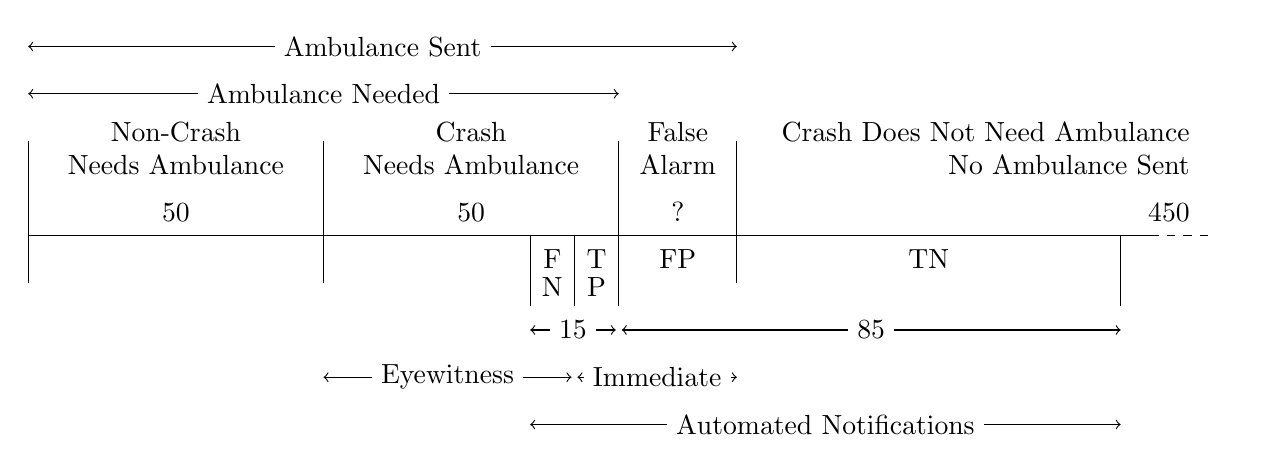
\begin{tikzpicture}[x=0.075cm, y=0.6cm, font=\normalfont\normalsize] % 15 cm wide
	\path (207,0) circle (0pt);
	\draw [color=black] (0,0) -- (190,0);
	\draw [color=black, dashed] (190,0) -- (200,0);
	\draw [color=black] (0,2) -- (0,-1);
	\draw [color=black] (50,2) -- (50,-1);
	\draw [color=black] (100,2) -- (100,-1.5);
	\draw [color=black] (120,2) -- (120,-1);
	\node (A) at (25,0) {};
	\node (B) [above=-2pt of A, align=center, text=black] {
		Non-Crash \\ Needs Ambulance \\[0.5em] 50
	};
	\node (C) at (75,0) {};
	\node (D) [above=-2pt of C, align=center, text=black] {
		Crash \\ Needs Ambulance \\[0.5em] 50
	};
	\node (E) at (200,0) {};
	\node (F) [above left =-2pt and 0pt of E, align=right, text=black] {
		Crash Does Not Need Ambulance \\ No Ambulance Sent \\[0.5em] 450
	};
	\node (G) at (110,0) {};
	\node (H) [above=-2pt of G, align=center, text=black] {
		False \\ Alarm \\[0.5em] ?
	};

	\draw [color=black] (85,0) -- (85,-1.5);
	\draw [color=black] (185,0) -- (185,-1.5);
%	\path (85,-2) -- (100,-2) node [below, midway, color=black] {15};
%	\path (100,-1) -- (185,-1) node [below, midway, color=black] {85};
	
	\draw [<->, color=black]  (100.5,-2) -- (185,-2) 
		node [midway, color=black, fill=white, align=center] 
		{85};

	\draw [<->, color=black]  (85,-2) -- (99.5,-2) 
		node [midway, color=black, fill=white, align=center] 
		{15};

	\draw [<->, color=black]  (50,-3) -- (92,-3) 
		node [midway, color=black, fill=white, align=center] 
		{Eyewitness};

	\draw [<->, color=black]  (93,-3) -- (120,-3) 
		node [midway, color=black, fill=white, align=center] 
		{Immediate};

	\draw [<->, color=black]  (85,-4) -- (185,-4) 
		node [midway, color=black, fill=white, align=center] 
		{Automated Notifications};

	\draw [<->, color=black]  (0,3) -- (100,3) 
		node [midway, color=black, fill=white, align=center] 
		{Ambulance Needed};

	\draw [<->, color=black]  (0,4) -- (120,4) 
		node [midway, color=black, fill=white, align=center] 
		{Ambulance Sent};

%	\node (G) at (110,2) [color=black, align=left] {False \\  Alarm};
	\path (100,-0.5) -- (120,-0.5) node [midway, color=black] {FP};
	\path (120,-0.5) -- (185,-0.5) node [midway, color=black] {TN};
	\draw [color=black] (92.5,0) -- (92.5,-1.5);
	\path (85,-0.5) -- (92.5,-0.5) node [midway, color=black] {F};
	\path (85,-1.2) -- (92.5,-1.0) node [midway, color=black] {N};
	\path (100,-0.5) -- (92.5,-0.5) node [midway, color=black] {T};
	\path (100,-1.2) -- (92.5,-1.0) node [midway, color=black] {P};
\end{tikzpicture}

\caption{\normalfont\normalsize Springfield after implementing immediate dispatch of ambulances.  Figure accompanies \S\ref{intro_scenario}}
\label{methods_springfield_after}
\end{figure}

\FloatBarrier




%%%%%
\subsubsection{Budgetary Decision Metric I:  Percent Increased Number of Ambulance Calls}
\label{political_decisions_percent_increased}

When a city or region implements immediate dispatch of ambulances, the number of ambulance dispatches increases by FP.   Within the automated notifications, 
$\text{P} = \text{FN} + \text{TP}$
 ambulance runs becomes P + FP = FN + TP + FP ambulance runs, an increase by a rate of $\text{FP}/\text{P}$.  The increase does not include the true positives (TP), because those ambulances would go eventually with or without immediate dispatch; the increase is the number of false positives (FP).  
 
In the short term (too short to buy more ambulances and hire more teams), the existing budget can support an increase of the number of ambulance runs to crash persons by some small percentage.  In the longer term, the city is willing to increase the budget to increase the number of ambulances going to crashes with automated notifications by a larger, but still fixed, percentage.  We will use 5\% as our example of how to implement this policy.   
  
 In our Springfield scenario, scaling to 100 currently sent ambulances to crash or non-crash, the total number of ambulance runs goes from 100 to 100 + FP, a rate of increase of $\text{FP}/100$.  For any city or region, if we knew the proportion of crashes with automated notifications from cell phones and the proportion of ambulances going to crashes, we could choose an
 $\text{FP}/\text{P}$
 threshold to match a budgetary decision criterion based on the increase in total number of ambulances sent to crashes or total number of ambulances sent to any situation.

Set the decision threshold $\theta$ where the number of false positives is 5\% of the positive class.  

\begin{equation} \label{eq:budget_1}\hfil
\frac{ \text{FP}}{\text{P}}
=
\frac{ \text{FP}}{\text{FN} + \text{TP}}
= 0.05
\end{equation}

%%%%%
\subsubsection{Budgetary Decision Metric II:  Percent of Immediately Dispatched Ambulances Actually Needed}
\label{political_decisions_precision}

A city or region is willing to immediately dispatch ambulances based on automated crash reports, but only up to the point where a certain proportion of the ambulances they immediately dispatch 
$(\text{PP} = \text{FP} + \text{TP})$ 
are actually needed (TP).  This proportion, 
$\text{TP}/(\text{FP} + \text{TP})$ 
is called the {\it precision} of a machine learning model.

To illustrate the method, we will choose $\text{Precision} = 2/3$, being willing to immediately dispatch one unnecessary ambulance for each two necessary ones.

\begin{equation} \label{eq:budget_2}\hfil
\frac{ \text{TP}}{\text{PP}}
=
\frac{ \text{TP}}{\text{FP} + \text{TP}}
= \frac{2}{3}
\end{equation}

%%%%%
\subsubsection{Budgetary Decision Metric III:  Minimum Probability that Each Immediately Dispatched Ambulance is Needed}
\label{political_decisions_probability}

The previous two decision criteria let the city leaders choose a specific dollar amount of increase in the annual ambulance budget, but for ethical reasons they may decide that, while they cannot afford to immediately dispatch an ambulance to every crash notification, they should immediately dispatch an ambulance to a crash notification with some probability (like 50\% or 80\%) of needing medical attention, and consider the total cost later.  

Our recommendation system will use a supervised-learning binary classification model trained on historical data. The models do not actually return a probability for each sample.  The models return, for each sample, a value $p$ that, generally, increases with the probability.  For each sample we also know whether that historical crash person actually needed an ambulance, whether that sample is in the negative or positive class.  

Consider a small band of values $p \in [\theta, \theta + \delta)$.  The samples in that band of $p$ are either in the negative or positive class.  Call the number of negative and positive samples in the band Neg and Pos, to distinguish from the total number of samples in the negative and positive classes, N and P.  The probability that a crash person in that band of $p$ needs an ambulance is given by 
$\text{Pos}/(\text{Neg} + \text{Pos})$.  

Since we have a discrete data set, not a smooth continuous function, if $\delta$ is too small, we will see the underlying randomness and the probability we calculate will not be an increasing function of $p$.  Larger values of $\delta$ would smooth out the randomness but give us less fine control.  The ideal $\delta$ is the smallest value that makes the probability increase with $p$.   Since some of our models give $p$ rounded to two decimal places, and because it is sufficiently small to illustrate the method, we will generally choose $\delta = 0.01$.  

To illustrate the method, we will choose the minimum marginal probability to be 50\%, meaning that each ambulance we immediately dispatch has at least a fifty percent chance of being needed.  We will find the least value of $\theta$ such that in the band $p \in [\theta - \delta, \theta + \delta)$, 

\begin{equation} \label{eq:budget_3}\hfil
\frac{\text{Pos}}{\text{Neg}+\text{Pos}} \ge 0.5
\end{equation}

\noindent and recommend immediately dispatching an ambulance to each automatic notification for which our model returns $p \ge \theta$.

We can relate this metric to a familiar metric if we rephrase the probability as the ratio of needed to unneeded ambulances immediately dispatched.  For instance, a 50\% probability is a 1:1 ratio of needed to unneeded, and an 80\% probability is a 4:1 ratio of needed to unneeded.  
The proportion of needed to unneeded ambulances sent in a neighborhood of $p$ is proportional to a widely used metric, the slope of the ROC curve, with the constant of proportionality being the class ratio.  

\begin{equation} \label{eq:ROC_slope}\hfil
\frac{\text{Pos}}{\text{Neg}}
=\frac{\Delta\text{TP}}{\Delta \text{FP}}
=\frac{\text{P}}{\text{N}} \cdot \frac{\Delta\text{TP}/\text{P}}{\Delta \text{FP}/\text{N}} 
=\frac{\text{P}}{\text{N}} \cdot \frac{\Delta\text{TPR}}{\Delta \text{FPR}}
=\frac{\text{P}}{\text{N}} \cdot m\text{ROC}
\end{equation}






\subsection{Dataset}
\label{dataset}

Ideally, we would use a dataset of crashes that spawned an automated notification, but we have not found such a dataset that is publicly available.  Working with such a private dataset would be an important avenue of future research. (See \S \ref{simplifying_assumptions} for a list of simplifying assumptions and opportunities for future research.)

We will use the Crash Report Sampling System (CRSS) data from 2016 to 2021.  The CRSS is a curated sample of crashes in the US, weighted to more serious crashes such that 17\% of the crash persons needed an ambulance, significantly more than the proportion of all reported crashes needing an ambulance.  Since many low-speed crashes would have a crash profile similar to hard braking, they would not spawn an automated notification, so it is reasonable to assume that the set of crashes with automated notifications would have a higher percentage of persons needing an ambulance.  

We make some simplifying assumptions (see \S\ref{simplifying_assumptions}) using this dataset, including that the class ratio (P:N) in the automated crash notification from cell phones will be close to that in the CRSS data, 1:5, and that the crash persons in the CRSS data are representative of the future crash persons whose cell phones send a crash notification.  

We will use the CRSS as a proxy for the set of crashes with automatic crash notifications, acknowledging that we do not know how good of a proxy it is. The primary merit of CRSS for our work is that it is publicly available so that our work can be critiqued, adapted, and expanded by others.  

To prepare the data we had to bin (discretize) some features and to impute missing data.  Some features in CRSS have both the original data with values signifying ``Missing'' or ``Unknown'' and a new feature with missing values imputed using IVEware \citep{IVEware}, but not all of the features we wanted to use had imputed values \citep{CRSS_Imputation}, so we compared several methods .  We debated the proper order of operations for binning and imputing, tried both, and decided to bin first, then imputed using a round-robin random forest method.  We removed all crashes involving a pedestrian because deceleration profile of such a crash would be more like hard braking than hitting a large immovable object like a car or tree, so less likely to trigger an automated notification.  

The dataset is slightly imbalanced, with five element of the negative class for each element of the positive class.  We considered several methods to handle the imbalance, including resampling, class weights, focal loss \citep{lin2017focal}, and balanced metrics.  We cannot use the popular SMOTE oversampling method because our data is categorical \citep{Chawla_2002}.  We tried undersampling with Tomek Links, but the resulting model results were not significantly different.  The best results came from using the model algorithms from Imbalanced-Learn \citep{Imblearn}, some of which apply bagging on top of algorithms from Scikit-Learn \citep{scikit-learn}.

After removing those pedestrian crashes we had 713,566 samples, each representing a crash person, and 78 relevant features.  For details, see these sections of code at 
\url{www.github.com/bburkman/Ambulance_Dispatch}.

\

\begin{tabular}{l}
	\verb|Ambulance_Dispatch_01_Get_Data.ipynb| \cr
	\verb|Ambulance_Dispatch_02_Correlation.ipynb| \cr
	\verb|Ambulance_Dispatch_03_Bin_Data.ipynb| \cr
	\verb|Ambulance_Dispatch_04_Impute_Missing_Data.ipynb| \cr
	\verb|Ambulance_Dispatch_05_IVEware_Order_of_Operations.ipynb| \cr
	\verb|Ambulance_Dispatch_06_Build_Models_Tomek_Links.ipynb| \cr
\end{tabular}



\subsection{Choosing Features}
\label{features}

The \verb|Accident|, \verb|Vehicle|, and \verb|Person| files of the CRSS dataset 2016-2021 have 170 unique features.  

First we narrowed the features to those that are relevant, of good quality, and knowable at the time of the automated notification (before any eyewitness reports).  Some features, like Vehicle Identification Number (VIN), have no predictive value.  Other features have missing data for more than 20\% of samples.  Some features, like drug and alcohol test results, are unknowable at the time of the automated notification.

Having data available for instantaneous analysis when the crash notification arrives is not free, and some features are more expensive than others.  A city thinking of implementing a recommendation system for immediate dispatch would need to decide how much to spend to have the data available, and whether the more expensive features increase the quality of the models enough to be worth the cost.  We categorized the features as ``Easy,'' ``Medium,'' and ``Hard,'' which can also be called ``Free,'' ``Expensive,'' and ``Problematic.''   The ``Easy'' features are those the dispatcher already has, like day of week, time of day, weather, and urban/rural.  The ``Medium'' features add details about the location (intersection, speed limit, interstate highway) and information the cell service company probably has about the primary user of the phone (age and sex).  To have the medium features instantaneously available would require coordination of many resources and be expensive to set up.  The ``Hard'' features are much more problematic, requiring more coordination of public and private records, and having that data readily available introduces privacy and data security concerns.  Hard features include whether the location is a work zone, the likely vehicle driven by the primary user of the cell phone, and, if there are multiple automated notifications from the same location, how many crash persons are likely to be involved.   

We note here our simplifying assumption (\S \ref{simplifying_assumptions}) that we will have complete and accurate data for each automated notification.  Also, we will test three combinations of features but have not done more detailed testing to see which individual features or other groupings of features are most or least useful in predicting whether a crash person needs an ambulance.  

See 
\verb|Ambulance_Dispatch_01_Get_Data.ipynb|  
for a list of the excluded features.

See \verb|Ambulance_Dispatch_03_Bin_Data.ipynb|
for a list of the features we used for imputation of missing data in CRSS.


See
\verb|Ambulance_Dispatch_07_Build_Models.ipynb|.
for the complete list of the features used in the Easy, Medium, and Hard model building.
\subsection{Models}
\label{models}

See \verb|Ambulance_Dispatch_07_Build_Models.ipynb| for more details.  

%%%%%
\FloatBarrier
\subsubsection{Binary Classification Algorithms and Hyperparameters}
\label{algorithms}

For each of the three sets of features we used eight binary classification algorithms, three of which take class weight $\alpha$ and one of which takes the focal loss parameter $\gamma$.  (See Table \ref{models}) We learned models for various values of the hyperparameters, giving $3 \times 13 = 39$ different models.  The $\alpha=0.5$ class weight is the default, and the $\alpha = 0.85$ class weight balances the effect of the negative and positive class in the loss function, as 85\% of the samples are in the negative class.  Focal loss \citep{lin2017focal} puts more weight in the loss function on the samples that are badly classified, much like least squares regression puts more weight on the points furthest from the line.  Setting $\gamma=0.0$ has no effect; Lin's paper tested from $\gamma=0.5$ to $\gamma = 5.0$ and recommended $\gamma = 2.0$.  

\

\begin{table}[h]
\label{models}
\caption{\normalsize\normalfont Models Tested for Recommendation System.  Table accompanies \S \ref{algorithms}}
\centering
\normalsize\normalfont
\begin{tabular}{lllcc}
&&& \bf Class &\bf Focal  \cr
\bf Model & \bf Abbreviation&\bf Source &\bf Weight $\alpha$ &\bf Loss $\gamma$ \cr\hline

AdaBoost  Classifier & AdaBoost & Scikit-Learn &  \cr\hline

Balanced Bagging Classifier & Bal Bag & Imbalanced-Learn &  \cr\hline

Balanced Random Forest Classifier & Bal RF & Imbalanced-Learn & 0.5 \cr
	&&& 0.85 \cr\hline

Easy Ensemble Classifier with AdaBoost Estimator & Easy Ens & Imbalanced-Learn &  \cr\hline

KerasClassifier with the  & Keras & Keras & 0.5 & 0.0 \cr
\qquad Binary Focal Crossentropy loss function &&& 0.5 & 1.0  \cr
	&&& 0.5 & 2.0 \cr
	&&& 0.85 & 0.0 \cr\hline

Logistic Regression Classifier & Log Reg & Scikit-Learn & 0.5 \cr
	&&& 0.85 \cr\hline

Random Forest Classifier & RF & Scikit-Learn &  \cr\hline

RUSBoost Classifier & RUSBoost & Imbalanced-Learn &  \cr

\end{tabular}
\end{table}

\FloatBarrier

\subsubsection{Hyperparameter Effects}
\label{hyperparameters}

Our experience with varying the class weight and focal loss parameters was that they shifted the entire $p$ distribution, both the positive and negative class, but did not do a better job of separating the positive and negative class, as measured by the area under the curve (AUC) of the receiver operating characteristic (ROC), as illustrated in Figure \ref{hyperparameters_figure} below. 

The KerasClassifier with the Binary Focal Crossentropy loss function takes both a class weight parameter $\alpha$ and a focal loss parameter $\gamma$.  Varying these parameters gave us different shapes of distributions of $p$, but all three versions of the model on the hard features had ROC AUC between 0.7781 and 0.7785, a difference within the normal ranges of randomness in machine learning models.  

If one is using the default decision threshold $\theta = 0.5$, then these hyperparameters are useful for shifting the distribution to meet the threshold, but since we are taking the liberty to move the threshold, varying the hyperparameters may be of little use.  Since the ROC AUC quantifies how well the algorithm separates the positive and negative classes over the whole range of $p$, and we are most interested in a small range of $p$ on the right end, the weights may yet have some useful effect, a topic for future investigation (\S\ref{simplifying_assumptions}).


\

%%%
\begin{figure}[h]
\noindent\begin{tabular}{@{\hspace{-6pt}}p{2.3in} @{\hspace{-6pt}}p{2.3in} @{\hspace{-6pt}}p{2.3in} }
	\vskip 0pt
	\hfil {\normalfont\normalsize $\alpha = 0.5$, $\gamma = 0.0$}
	
	
	%% Creator: Matplotlib, PGF backend
%%
%% To include the figure in your LaTeX document, write
%%   \input{<filename>.pgf}
%%
%% Make sure the required packages are loaded in your preamble
%%   \usepackage{pgf}
%%
%% Also ensure that all the required font packages are loaded; for instance,
%% the lmodern package is sometimes necessary when using math font.
%%   \usepackage{lmodern}
%%
%% Figures using additional raster images can only be included by \input if
%% they are in the same directory as the main LaTeX file. For loading figures
%% from other directories you can use the `import` package
%%   \usepackage{import}
%%
%% and then include the figures with
%%   \import{<path to file>}{<filename>.pgf}
%%
%% Matplotlib used the following preamble
%%   
%%   \usepackage{fontspec}
%%   \makeatletter\@ifpackageloaded{underscore}{}{\usepackage[strings]{underscore}}\makeatother
%%
\begingroup%
\makeatletter%
\begin{pgfpicture}%
\pgfpathrectangle{\pgfpointorigin}{\pgfqpoint{2.153750in}{1.654444in}}%
\pgfusepath{use as bounding box, clip}%
\begin{pgfscope}%
\pgfsetbuttcap%
\pgfsetmiterjoin%
\definecolor{currentfill}{rgb}{1.000000,1.000000,1.000000}%
\pgfsetfillcolor{currentfill}%
\pgfsetlinewidth{0.000000pt}%
\definecolor{currentstroke}{rgb}{1.000000,1.000000,1.000000}%
\pgfsetstrokecolor{currentstroke}%
\pgfsetdash{}{0pt}%
\pgfpathmoveto{\pgfqpoint{0.000000in}{0.000000in}}%
\pgfpathlineto{\pgfqpoint{2.153750in}{0.000000in}}%
\pgfpathlineto{\pgfqpoint{2.153750in}{1.654444in}}%
\pgfpathlineto{\pgfqpoint{0.000000in}{1.654444in}}%
\pgfpathlineto{\pgfqpoint{0.000000in}{0.000000in}}%
\pgfpathclose%
\pgfusepath{fill}%
\end{pgfscope}%
\begin{pgfscope}%
\pgfsetbuttcap%
\pgfsetmiterjoin%
\definecolor{currentfill}{rgb}{1.000000,1.000000,1.000000}%
\pgfsetfillcolor{currentfill}%
\pgfsetlinewidth{0.000000pt}%
\definecolor{currentstroke}{rgb}{0.000000,0.000000,0.000000}%
\pgfsetstrokecolor{currentstroke}%
\pgfsetstrokeopacity{0.000000}%
\pgfsetdash{}{0pt}%
\pgfpathmoveto{\pgfqpoint{0.465000in}{0.449444in}}%
\pgfpathlineto{\pgfqpoint{2.015000in}{0.449444in}}%
\pgfpathlineto{\pgfqpoint{2.015000in}{1.604444in}}%
\pgfpathlineto{\pgfqpoint{0.465000in}{1.604444in}}%
\pgfpathlineto{\pgfqpoint{0.465000in}{0.449444in}}%
\pgfpathclose%
\pgfusepath{fill}%
\end{pgfscope}%
\begin{pgfscope}%
\pgfpathrectangle{\pgfqpoint{0.465000in}{0.449444in}}{\pgfqpoint{1.550000in}{1.155000in}}%
\pgfusepath{clip}%
\pgfsetbuttcap%
\pgfsetmiterjoin%
\pgfsetlinewidth{1.003750pt}%
\definecolor{currentstroke}{rgb}{0.000000,0.000000,0.000000}%
\pgfsetstrokecolor{currentstroke}%
\pgfsetdash{}{0pt}%
\pgfpathmoveto{\pgfqpoint{0.455000in}{0.449444in}}%
\pgfpathlineto{\pgfqpoint{0.502805in}{0.449444in}}%
\pgfpathlineto{\pgfqpoint{0.502805in}{1.549444in}}%
\pgfpathlineto{\pgfqpoint{0.455000in}{1.549444in}}%
\pgfusepath{stroke}%
\end{pgfscope}%
\begin{pgfscope}%
\pgfpathrectangle{\pgfqpoint{0.465000in}{0.449444in}}{\pgfqpoint{1.550000in}{1.155000in}}%
\pgfusepath{clip}%
\pgfsetbuttcap%
\pgfsetmiterjoin%
\pgfsetlinewidth{1.003750pt}%
\definecolor{currentstroke}{rgb}{0.000000,0.000000,0.000000}%
\pgfsetstrokecolor{currentstroke}%
\pgfsetdash{}{0pt}%
\pgfpathmoveto{\pgfqpoint{0.593537in}{0.449444in}}%
\pgfpathlineto{\pgfqpoint{0.654025in}{0.449444in}}%
\pgfpathlineto{\pgfqpoint{0.654025in}{0.933540in}}%
\pgfpathlineto{\pgfqpoint{0.593537in}{0.933540in}}%
\pgfpathlineto{\pgfqpoint{0.593537in}{0.449444in}}%
\pgfpathclose%
\pgfusepath{stroke}%
\end{pgfscope}%
\begin{pgfscope}%
\pgfpathrectangle{\pgfqpoint{0.465000in}{0.449444in}}{\pgfqpoint{1.550000in}{1.155000in}}%
\pgfusepath{clip}%
\pgfsetbuttcap%
\pgfsetmiterjoin%
\pgfsetlinewidth{1.003750pt}%
\definecolor{currentstroke}{rgb}{0.000000,0.000000,0.000000}%
\pgfsetstrokecolor{currentstroke}%
\pgfsetdash{}{0pt}%
\pgfpathmoveto{\pgfqpoint{0.744756in}{0.449444in}}%
\pgfpathlineto{\pgfqpoint{0.805244in}{0.449444in}}%
\pgfpathlineto{\pgfqpoint{0.805244in}{0.658309in}}%
\pgfpathlineto{\pgfqpoint{0.744756in}{0.658309in}}%
\pgfpathlineto{\pgfqpoint{0.744756in}{0.449444in}}%
\pgfpathclose%
\pgfusepath{stroke}%
\end{pgfscope}%
\begin{pgfscope}%
\pgfpathrectangle{\pgfqpoint{0.465000in}{0.449444in}}{\pgfqpoint{1.550000in}{1.155000in}}%
\pgfusepath{clip}%
\pgfsetbuttcap%
\pgfsetmiterjoin%
\pgfsetlinewidth{1.003750pt}%
\definecolor{currentstroke}{rgb}{0.000000,0.000000,0.000000}%
\pgfsetstrokecolor{currentstroke}%
\pgfsetdash{}{0pt}%
\pgfpathmoveto{\pgfqpoint{0.895976in}{0.449444in}}%
\pgfpathlineto{\pgfqpoint{0.956464in}{0.449444in}}%
\pgfpathlineto{\pgfqpoint{0.956464in}{0.541436in}}%
\pgfpathlineto{\pgfqpoint{0.895976in}{0.541436in}}%
\pgfpathlineto{\pgfqpoint{0.895976in}{0.449444in}}%
\pgfpathclose%
\pgfusepath{stroke}%
\end{pgfscope}%
\begin{pgfscope}%
\pgfpathrectangle{\pgfqpoint{0.465000in}{0.449444in}}{\pgfqpoint{1.550000in}{1.155000in}}%
\pgfusepath{clip}%
\pgfsetbuttcap%
\pgfsetmiterjoin%
\pgfsetlinewidth{1.003750pt}%
\definecolor{currentstroke}{rgb}{0.000000,0.000000,0.000000}%
\pgfsetstrokecolor{currentstroke}%
\pgfsetdash{}{0pt}%
\pgfpathmoveto{\pgfqpoint{1.047195in}{0.449444in}}%
\pgfpathlineto{\pgfqpoint{1.107683in}{0.449444in}}%
\pgfpathlineto{\pgfqpoint{1.107683in}{0.492720in}}%
\pgfpathlineto{\pgfqpoint{1.047195in}{0.492720in}}%
\pgfpathlineto{\pgfqpoint{1.047195in}{0.449444in}}%
\pgfpathclose%
\pgfusepath{stroke}%
\end{pgfscope}%
\begin{pgfscope}%
\pgfpathrectangle{\pgfqpoint{0.465000in}{0.449444in}}{\pgfqpoint{1.550000in}{1.155000in}}%
\pgfusepath{clip}%
\pgfsetbuttcap%
\pgfsetmiterjoin%
\pgfsetlinewidth{1.003750pt}%
\definecolor{currentstroke}{rgb}{0.000000,0.000000,0.000000}%
\pgfsetstrokecolor{currentstroke}%
\pgfsetdash{}{0pt}%
\pgfpathmoveto{\pgfqpoint{1.198415in}{0.449444in}}%
\pgfpathlineto{\pgfqpoint{1.258903in}{0.449444in}}%
\pgfpathlineto{\pgfqpoint{1.258903in}{0.470608in}}%
\pgfpathlineto{\pgfqpoint{1.198415in}{0.470608in}}%
\pgfpathlineto{\pgfqpoint{1.198415in}{0.449444in}}%
\pgfpathclose%
\pgfusepath{stroke}%
\end{pgfscope}%
\begin{pgfscope}%
\pgfpathrectangle{\pgfqpoint{0.465000in}{0.449444in}}{\pgfqpoint{1.550000in}{1.155000in}}%
\pgfusepath{clip}%
\pgfsetbuttcap%
\pgfsetmiterjoin%
\pgfsetlinewidth{1.003750pt}%
\definecolor{currentstroke}{rgb}{0.000000,0.000000,0.000000}%
\pgfsetstrokecolor{currentstroke}%
\pgfsetdash{}{0pt}%
\pgfpathmoveto{\pgfqpoint{1.349634in}{0.449444in}}%
\pgfpathlineto{\pgfqpoint{1.410122in}{0.449444in}}%
\pgfpathlineto{\pgfqpoint{1.410122in}{0.459784in}}%
\pgfpathlineto{\pgfqpoint{1.349634in}{0.459784in}}%
\pgfpathlineto{\pgfqpoint{1.349634in}{0.449444in}}%
\pgfpathclose%
\pgfusepath{stroke}%
\end{pgfscope}%
\begin{pgfscope}%
\pgfpathrectangle{\pgfqpoint{0.465000in}{0.449444in}}{\pgfqpoint{1.550000in}{1.155000in}}%
\pgfusepath{clip}%
\pgfsetbuttcap%
\pgfsetmiterjoin%
\pgfsetlinewidth{1.003750pt}%
\definecolor{currentstroke}{rgb}{0.000000,0.000000,0.000000}%
\pgfsetstrokecolor{currentstroke}%
\pgfsetdash{}{0pt}%
\pgfpathmoveto{\pgfqpoint{1.500854in}{0.449444in}}%
\pgfpathlineto{\pgfqpoint{1.561342in}{0.449444in}}%
\pgfpathlineto{\pgfqpoint{1.561342in}{0.454465in}}%
\pgfpathlineto{\pgfqpoint{1.500854in}{0.454465in}}%
\pgfpathlineto{\pgfqpoint{1.500854in}{0.449444in}}%
\pgfpathclose%
\pgfusepath{stroke}%
\end{pgfscope}%
\begin{pgfscope}%
\pgfpathrectangle{\pgfqpoint{0.465000in}{0.449444in}}{\pgfqpoint{1.550000in}{1.155000in}}%
\pgfusepath{clip}%
\pgfsetbuttcap%
\pgfsetmiterjoin%
\pgfsetlinewidth{1.003750pt}%
\definecolor{currentstroke}{rgb}{0.000000,0.000000,0.000000}%
\pgfsetstrokecolor{currentstroke}%
\pgfsetdash{}{0pt}%
\pgfpathmoveto{\pgfqpoint{1.652073in}{0.449444in}}%
\pgfpathlineto{\pgfqpoint{1.712561in}{0.449444in}}%
\pgfpathlineto{\pgfqpoint{1.712561in}{0.451230in}}%
\pgfpathlineto{\pgfqpoint{1.652073in}{0.451230in}}%
\pgfpathlineto{\pgfqpoint{1.652073in}{0.449444in}}%
\pgfpathclose%
\pgfusepath{stroke}%
\end{pgfscope}%
\begin{pgfscope}%
\pgfpathrectangle{\pgfqpoint{0.465000in}{0.449444in}}{\pgfqpoint{1.550000in}{1.155000in}}%
\pgfusepath{clip}%
\pgfsetbuttcap%
\pgfsetmiterjoin%
\pgfsetlinewidth{1.003750pt}%
\definecolor{currentstroke}{rgb}{0.000000,0.000000,0.000000}%
\pgfsetstrokecolor{currentstroke}%
\pgfsetdash{}{0pt}%
\pgfpathmoveto{\pgfqpoint{1.803293in}{0.449444in}}%
\pgfpathlineto{\pgfqpoint{1.863781in}{0.449444in}}%
\pgfpathlineto{\pgfqpoint{1.863781in}{0.449613in}}%
\pgfpathlineto{\pgfqpoint{1.803293in}{0.449613in}}%
\pgfpathlineto{\pgfqpoint{1.803293in}{0.449444in}}%
\pgfpathclose%
\pgfusepath{stroke}%
\end{pgfscope}%
\begin{pgfscope}%
\pgfpathrectangle{\pgfqpoint{0.465000in}{0.449444in}}{\pgfqpoint{1.550000in}{1.155000in}}%
\pgfusepath{clip}%
\pgfsetbuttcap%
\pgfsetmiterjoin%
\definecolor{currentfill}{rgb}{0.000000,0.000000,0.000000}%
\pgfsetfillcolor{currentfill}%
\pgfsetlinewidth{0.000000pt}%
\definecolor{currentstroke}{rgb}{0.000000,0.000000,0.000000}%
\pgfsetstrokecolor{currentstroke}%
\pgfsetstrokeopacity{0.000000}%
\pgfsetdash{}{0pt}%
\pgfpathmoveto{\pgfqpoint{0.502805in}{0.449444in}}%
\pgfpathlineto{\pgfqpoint{0.563293in}{0.449444in}}%
\pgfpathlineto{\pgfqpoint{0.563293in}{0.510244in}}%
\pgfpathlineto{\pgfqpoint{0.502805in}{0.510244in}}%
\pgfpathlineto{\pgfqpoint{0.502805in}{0.449444in}}%
\pgfpathclose%
\pgfusepath{fill}%
\end{pgfscope}%
\begin{pgfscope}%
\pgfpathrectangle{\pgfqpoint{0.465000in}{0.449444in}}{\pgfqpoint{1.550000in}{1.155000in}}%
\pgfusepath{clip}%
\pgfsetbuttcap%
\pgfsetmiterjoin%
\definecolor{currentfill}{rgb}{0.000000,0.000000,0.000000}%
\pgfsetfillcolor{currentfill}%
\pgfsetlinewidth{0.000000pt}%
\definecolor{currentstroke}{rgb}{0.000000,0.000000,0.000000}%
\pgfsetstrokecolor{currentstroke}%
\pgfsetstrokeopacity{0.000000}%
\pgfsetdash{}{0pt}%
\pgfpathmoveto{\pgfqpoint{0.654025in}{0.449444in}}%
\pgfpathlineto{\pgfqpoint{0.714512in}{0.449444in}}%
\pgfpathlineto{\pgfqpoint{0.714512in}{0.535204in}}%
\pgfpathlineto{\pgfqpoint{0.654025in}{0.535204in}}%
\pgfpathlineto{\pgfqpoint{0.654025in}{0.449444in}}%
\pgfpathclose%
\pgfusepath{fill}%
\end{pgfscope}%
\begin{pgfscope}%
\pgfpathrectangle{\pgfqpoint{0.465000in}{0.449444in}}{\pgfqpoint{1.550000in}{1.155000in}}%
\pgfusepath{clip}%
\pgfsetbuttcap%
\pgfsetmiterjoin%
\definecolor{currentfill}{rgb}{0.000000,0.000000,0.000000}%
\pgfsetfillcolor{currentfill}%
\pgfsetlinewidth{0.000000pt}%
\definecolor{currentstroke}{rgb}{0.000000,0.000000,0.000000}%
\pgfsetstrokecolor{currentstroke}%
\pgfsetstrokeopacity{0.000000}%
\pgfsetdash{}{0pt}%
\pgfpathmoveto{\pgfqpoint{0.805244in}{0.449444in}}%
\pgfpathlineto{\pgfqpoint{0.865732in}{0.449444in}}%
\pgfpathlineto{\pgfqpoint{0.865732in}{0.516878in}}%
\pgfpathlineto{\pgfqpoint{0.805244in}{0.516878in}}%
\pgfpathlineto{\pgfqpoint{0.805244in}{0.449444in}}%
\pgfpathclose%
\pgfusepath{fill}%
\end{pgfscope}%
\begin{pgfscope}%
\pgfpathrectangle{\pgfqpoint{0.465000in}{0.449444in}}{\pgfqpoint{1.550000in}{1.155000in}}%
\pgfusepath{clip}%
\pgfsetbuttcap%
\pgfsetmiterjoin%
\definecolor{currentfill}{rgb}{0.000000,0.000000,0.000000}%
\pgfsetfillcolor{currentfill}%
\pgfsetlinewidth{0.000000pt}%
\definecolor{currentstroke}{rgb}{0.000000,0.000000,0.000000}%
\pgfsetstrokecolor{currentstroke}%
\pgfsetstrokeopacity{0.000000}%
\pgfsetdash{}{0pt}%
\pgfpathmoveto{\pgfqpoint{0.956464in}{0.449444in}}%
\pgfpathlineto{\pgfqpoint{1.016951in}{0.449444in}}%
\pgfpathlineto{\pgfqpoint{1.016951in}{0.495562in}}%
\pgfpathlineto{\pgfqpoint{0.956464in}{0.495562in}}%
\pgfpathlineto{\pgfqpoint{0.956464in}{0.449444in}}%
\pgfpathclose%
\pgfusepath{fill}%
\end{pgfscope}%
\begin{pgfscope}%
\pgfpathrectangle{\pgfqpoint{0.465000in}{0.449444in}}{\pgfqpoint{1.550000in}{1.155000in}}%
\pgfusepath{clip}%
\pgfsetbuttcap%
\pgfsetmiterjoin%
\definecolor{currentfill}{rgb}{0.000000,0.000000,0.000000}%
\pgfsetfillcolor{currentfill}%
\pgfsetlinewidth{0.000000pt}%
\definecolor{currentstroke}{rgb}{0.000000,0.000000,0.000000}%
\pgfsetstrokecolor{currentstroke}%
\pgfsetstrokeopacity{0.000000}%
\pgfsetdash{}{0pt}%
\pgfpathmoveto{\pgfqpoint{1.107683in}{0.449444in}}%
\pgfpathlineto{\pgfqpoint{1.168171in}{0.449444in}}%
\pgfpathlineto{\pgfqpoint{1.168171in}{0.481594in}}%
\pgfpathlineto{\pgfqpoint{1.107683in}{0.481594in}}%
\pgfpathlineto{\pgfqpoint{1.107683in}{0.449444in}}%
\pgfpathclose%
\pgfusepath{fill}%
\end{pgfscope}%
\begin{pgfscope}%
\pgfpathrectangle{\pgfqpoint{0.465000in}{0.449444in}}{\pgfqpoint{1.550000in}{1.155000in}}%
\pgfusepath{clip}%
\pgfsetbuttcap%
\pgfsetmiterjoin%
\definecolor{currentfill}{rgb}{0.000000,0.000000,0.000000}%
\pgfsetfillcolor{currentfill}%
\pgfsetlinewidth{0.000000pt}%
\definecolor{currentstroke}{rgb}{0.000000,0.000000,0.000000}%
\pgfsetstrokecolor{currentstroke}%
\pgfsetstrokeopacity{0.000000}%
\pgfsetdash{}{0pt}%
\pgfpathmoveto{\pgfqpoint{1.258903in}{0.449444in}}%
\pgfpathlineto{\pgfqpoint{1.319391in}{0.449444in}}%
\pgfpathlineto{\pgfqpoint{1.319391in}{0.472641in}}%
\pgfpathlineto{\pgfqpoint{1.258903in}{0.472641in}}%
\pgfpathlineto{\pgfqpoint{1.258903in}{0.449444in}}%
\pgfpathclose%
\pgfusepath{fill}%
\end{pgfscope}%
\begin{pgfscope}%
\pgfpathrectangle{\pgfqpoint{0.465000in}{0.449444in}}{\pgfqpoint{1.550000in}{1.155000in}}%
\pgfusepath{clip}%
\pgfsetbuttcap%
\pgfsetmiterjoin%
\definecolor{currentfill}{rgb}{0.000000,0.000000,0.000000}%
\pgfsetfillcolor{currentfill}%
\pgfsetlinewidth{0.000000pt}%
\definecolor{currentstroke}{rgb}{0.000000,0.000000,0.000000}%
\pgfsetstrokecolor{currentstroke}%
\pgfsetstrokeopacity{0.000000}%
\pgfsetdash{}{0pt}%
\pgfpathmoveto{\pgfqpoint{1.410122in}{0.449444in}}%
\pgfpathlineto{\pgfqpoint{1.470610in}{0.449444in}}%
\pgfpathlineto{\pgfqpoint{1.470610in}{0.466302in}}%
\pgfpathlineto{\pgfqpoint{1.410122in}{0.466302in}}%
\pgfpathlineto{\pgfqpoint{1.410122in}{0.449444in}}%
\pgfpathclose%
\pgfusepath{fill}%
\end{pgfscope}%
\begin{pgfscope}%
\pgfpathrectangle{\pgfqpoint{0.465000in}{0.449444in}}{\pgfqpoint{1.550000in}{1.155000in}}%
\pgfusepath{clip}%
\pgfsetbuttcap%
\pgfsetmiterjoin%
\definecolor{currentfill}{rgb}{0.000000,0.000000,0.000000}%
\pgfsetfillcolor{currentfill}%
\pgfsetlinewidth{0.000000pt}%
\definecolor{currentstroke}{rgb}{0.000000,0.000000,0.000000}%
\pgfsetstrokecolor{currentstroke}%
\pgfsetstrokeopacity{0.000000}%
\pgfsetdash{}{0pt}%
\pgfpathmoveto{\pgfqpoint{1.561342in}{0.449444in}}%
\pgfpathlineto{\pgfqpoint{1.621830in}{0.449444in}}%
\pgfpathlineto{\pgfqpoint{1.621830in}{0.461207in}}%
\pgfpathlineto{\pgfqpoint{1.561342in}{0.461207in}}%
\pgfpathlineto{\pgfqpoint{1.561342in}{0.449444in}}%
\pgfpathclose%
\pgfusepath{fill}%
\end{pgfscope}%
\begin{pgfscope}%
\pgfpathrectangle{\pgfqpoint{0.465000in}{0.449444in}}{\pgfqpoint{1.550000in}{1.155000in}}%
\pgfusepath{clip}%
\pgfsetbuttcap%
\pgfsetmiterjoin%
\definecolor{currentfill}{rgb}{0.000000,0.000000,0.000000}%
\pgfsetfillcolor{currentfill}%
\pgfsetlinewidth{0.000000pt}%
\definecolor{currentstroke}{rgb}{0.000000,0.000000,0.000000}%
\pgfsetstrokecolor{currentstroke}%
\pgfsetstrokeopacity{0.000000}%
\pgfsetdash{}{0pt}%
\pgfpathmoveto{\pgfqpoint{1.712561in}{0.449444in}}%
\pgfpathlineto{\pgfqpoint{1.773049in}{0.449444in}}%
\pgfpathlineto{\pgfqpoint{1.773049in}{0.455312in}}%
\pgfpathlineto{\pgfqpoint{1.712561in}{0.455312in}}%
\pgfpathlineto{\pgfqpoint{1.712561in}{0.449444in}}%
\pgfpathclose%
\pgfusepath{fill}%
\end{pgfscope}%
\begin{pgfscope}%
\pgfpathrectangle{\pgfqpoint{0.465000in}{0.449444in}}{\pgfqpoint{1.550000in}{1.155000in}}%
\pgfusepath{clip}%
\pgfsetbuttcap%
\pgfsetmiterjoin%
\definecolor{currentfill}{rgb}{0.000000,0.000000,0.000000}%
\pgfsetfillcolor{currentfill}%
\pgfsetlinewidth{0.000000pt}%
\definecolor{currentstroke}{rgb}{0.000000,0.000000,0.000000}%
\pgfsetstrokecolor{currentstroke}%
\pgfsetstrokeopacity{0.000000}%
\pgfsetdash{}{0pt}%
\pgfpathmoveto{\pgfqpoint{1.863781in}{0.449444in}}%
\pgfpathlineto{\pgfqpoint{1.924269in}{0.449444in}}%
\pgfpathlineto{\pgfqpoint{1.924269in}{0.450084in}}%
\pgfpathlineto{\pgfqpoint{1.863781in}{0.450084in}}%
\pgfpathlineto{\pgfqpoint{1.863781in}{0.449444in}}%
\pgfpathclose%
\pgfusepath{fill}%
\end{pgfscope}%
\begin{pgfscope}%
\pgfsetbuttcap%
\pgfsetroundjoin%
\definecolor{currentfill}{rgb}{0.000000,0.000000,0.000000}%
\pgfsetfillcolor{currentfill}%
\pgfsetlinewidth{0.803000pt}%
\definecolor{currentstroke}{rgb}{0.000000,0.000000,0.000000}%
\pgfsetstrokecolor{currentstroke}%
\pgfsetdash{}{0pt}%
\pgfsys@defobject{currentmarker}{\pgfqpoint{0.000000in}{-0.048611in}}{\pgfqpoint{0.000000in}{0.000000in}}{%
\pgfpathmoveto{\pgfqpoint{0.000000in}{0.000000in}}%
\pgfpathlineto{\pgfqpoint{0.000000in}{-0.048611in}}%
\pgfusepath{stroke,fill}%
}%
\begin{pgfscope}%
\pgfsys@transformshift{0.502805in}{0.449444in}%
\pgfsys@useobject{currentmarker}{}%
\end{pgfscope}%
\end{pgfscope}%
\begin{pgfscope}%
\definecolor{textcolor}{rgb}{0.000000,0.000000,0.000000}%
\pgfsetstrokecolor{textcolor}%
\pgfsetfillcolor{textcolor}%
\pgftext[x=0.502805in,y=0.352222in,,top]{\color{textcolor}\rmfamily\fontsize{10.000000}{12.000000}\selectfont 0.0}%
\end{pgfscope}%
\begin{pgfscope}%
\pgfsetbuttcap%
\pgfsetroundjoin%
\definecolor{currentfill}{rgb}{0.000000,0.000000,0.000000}%
\pgfsetfillcolor{currentfill}%
\pgfsetlinewidth{0.803000pt}%
\definecolor{currentstroke}{rgb}{0.000000,0.000000,0.000000}%
\pgfsetstrokecolor{currentstroke}%
\pgfsetdash{}{0pt}%
\pgfsys@defobject{currentmarker}{\pgfqpoint{0.000000in}{-0.048611in}}{\pgfqpoint{0.000000in}{0.000000in}}{%
\pgfpathmoveto{\pgfqpoint{0.000000in}{0.000000in}}%
\pgfpathlineto{\pgfqpoint{0.000000in}{-0.048611in}}%
\pgfusepath{stroke,fill}%
}%
\begin{pgfscope}%
\pgfsys@transformshift{0.880854in}{0.449444in}%
\pgfsys@useobject{currentmarker}{}%
\end{pgfscope}%
\end{pgfscope}%
\begin{pgfscope}%
\definecolor{textcolor}{rgb}{0.000000,0.000000,0.000000}%
\pgfsetstrokecolor{textcolor}%
\pgfsetfillcolor{textcolor}%
\pgftext[x=0.880854in,y=0.352222in,,top]{\color{textcolor}\rmfamily\fontsize{10.000000}{12.000000}\selectfont 0.25}%
\end{pgfscope}%
\begin{pgfscope}%
\pgfsetbuttcap%
\pgfsetroundjoin%
\definecolor{currentfill}{rgb}{0.000000,0.000000,0.000000}%
\pgfsetfillcolor{currentfill}%
\pgfsetlinewidth{0.803000pt}%
\definecolor{currentstroke}{rgb}{0.000000,0.000000,0.000000}%
\pgfsetstrokecolor{currentstroke}%
\pgfsetdash{}{0pt}%
\pgfsys@defobject{currentmarker}{\pgfqpoint{0.000000in}{-0.048611in}}{\pgfqpoint{0.000000in}{0.000000in}}{%
\pgfpathmoveto{\pgfqpoint{0.000000in}{0.000000in}}%
\pgfpathlineto{\pgfqpoint{0.000000in}{-0.048611in}}%
\pgfusepath{stroke,fill}%
}%
\begin{pgfscope}%
\pgfsys@transformshift{1.258903in}{0.449444in}%
\pgfsys@useobject{currentmarker}{}%
\end{pgfscope}%
\end{pgfscope}%
\begin{pgfscope}%
\definecolor{textcolor}{rgb}{0.000000,0.000000,0.000000}%
\pgfsetstrokecolor{textcolor}%
\pgfsetfillcolor{textcolor}%
\pgftext[x=1.258903in,y=0.352222in,,top]{\color{textcolor}\rmfamily\fontsize{10.000000}{12.000000}\selectfont 0.5}%
\end{pgfscope}%
\begin{pgfscope}%
\pgfsetbuttcap%
\pgfsetroundjoin%
\definecolor{currentfill}{rgb}{0.000000,0.000000,0.000000}%
\pgfsetfillcolor{currentfill}%
\pgfsetlinewidth{0.803000pt}%
\definecolor{currentstroke}{rgb}{0.000000,0.000000,0.000000}%
\pgfsetstrokecolor{currentstroke}%
\pgfsetdash{}{0pt}%
\pgfsys@defobject{currentmarker}{\pgfqpoint{0.000000in}{-0.048611in}}{\pgfqpoint{0.000000in}{0.000000in}}{%
\pgfpathmoveto{\pgfqpoint{0.000000in}{0.000000in}}%
\pgfpathlineto{\pgfqpoint{0.000000in}{-0.048611in}}%
\pgfusepath{stroke,fill}%
}%
\begin{pgfscope}%
\pgfsys@transformshift{1.636951in}{0.449444in}%
\pgfsys@useobject{currentmarker}{}%
\end{pgfscope}%
\end{pgfscope}%
\begin{pgfscope}%
\definecolor{textcolor}{rgb}{0.000000,0.000000,0.000000}%
\pgfsetstrokecolor{textcolor}%
\pgfsetfillcolor{textcolor}%
\pgftext[x=1.636951in,y=0.352222in,,top]{\color{textcolor}\rmfamily\fontsize{10.000000}{12.000000}\selectfont 0.75}%
\end{pgfscope}%
\begin{pgfscope}%
\pgfsetbuttcap%
\pgfsetroundjoin%
\definecolor{currentfill}{rgb}{0.000000,0.000000,0.000000}%
\pgfsetfillcolor{currentfill}%
\pgfsetlinewidth{0.803000pt}%
\definecolor{currentstroke}{rgb}{0.000000,0.000000,0.000000}%
\pgfsetstrokecolor{currentstroke}%
\pgfsetdash{}{0pt}%
\pgfsys@defobject{currentmarker}{\pgfqpoint{0.000000in}{-0.048611in}}{\pgfqpoint{0.000000in}{0.000000in}}{%
\pgfpathmoveto{\pgfqpoint{0.000000in}{0.000000in}}%
\pgfpathlineto{\pgfqpoint{0.000000in}{-0.048611in}}%
\pgfusepath{stroke,fill}%
}%
\begin{pgfscope}%
\pgfsys@transformshift{2.015000in}{0.449444in}%
\pgfsys@useobject{currentmarker}{}%
\end{pgfscope}%
\end{pgfscope}%
\begin{pgfscope}%
\definecolor{textcolor}{rgb}{0.000000,0.000000,0.000000}%
\pgfsetstrokecolor{textcolor}%
\pgfsetfillcolor{textcolor}%
\pgftext[x=2.015000in,y=0.352222in,,top]{\color{textcolor}\rmfamily\fontsize{10.000000}{12.000000}\selectfont 1.0}%
\end{pgfscope}%
\begin{pgfscope}%
\definecolor{textcolor}{rgb}{0.000000,0.000000,0.000000}%
\pgfsetstrokecolor{textcolor}%
\pgfsetfillcolor{textcolor}%
\pgftext[x=1.240000in,y=0.173333in,,top]{\color{textcolor}\rmfamily\fontsize{10.000000}{12.000000}\selectfont \(\displaystyle p\)}%
\end{pgfscope}%
\begin{pgfscope}%
\pgfsetbuttcap%
\pgfsetroundjoin%
\definecolor{currentfill}{rgb}{0.000000,0.000000,0.000000}%
\pgfsetfillcolor{currentfill}%
\pgfsetlinewidth{0.803000pt}%
\definecolor{currentstroke}{rgb}{0.000000,0.000000,0.000000}%
\pgfsetstrokecolor{currentstroke}%
\pgfsetdash{}{0pt}%
\pgfsys@defobject{currentmarker}{\pgfqpoint{-0.048611in}{0.000000in}}{\pgfqpoint{-0.000000in}{0.000000in}}{%
\pgfpathmoveto{\pgfqpoint{-0.000000in}{0.000000in}}%
\pgfpathlineto{\pgfqpoint{-0.048611in}{0.000000in}}%
\pgfusepath{stroke,fill}%
}%
\begin{pgfscope}%
\pgfsys@transformshift{0.465000in}{0.449444in}%
\pgfsys@useobject{currentmarker}{}%
\end{pgfscope}%
\end{pgfscope}%
\begin{pgfscope}%
\definecolor{textcolor}{rgb}{0.000000,0.000000,0.000000}%
\pgfsetstrokecolor{textcolor}%
\pgfsetfillcolor{textcolor}%
\pgftext[x=0.298333in, y=0.401250in, left, base]{\color{textcolor}\rmfamily\fontsize{10.000000}{12.000000}\selectfont \(\displaystyle {0}\)}%
\end{pgfscope}%
\begin{pgfscope}%
\pgfsetbuttcap%
\pgfsetroundjoin%
\definecolor{currentfill}{rgb}{0.000000,0.000000,0.000000}%
\pgfsetfillcolor{currentfill}%
\pgfsetlinewidth{0.803000pt}%
\definecolor{currentstroke}{rgb}{0.000000,0.000000,0.000000}%
\pgfsetstrokecolor{currentstroke}%
\pgfsetdash{}{0pt}%
\pgfsys@defobject{currentmarker}{\pgfqpoint{-0.048611in}{0.000000in}}{\pgfqpoint{-0.000000in}{0.000000in}}{%
\pgfpathmoveto{\pgfqpoint{-0.000000in}{0.000000in}}%
\pgfpathlineto{\pgfqpoint{-0.048611in}{0.000000in}}%
\pgfusepath{stroke,fill}%
}%
\begin{pgfscope}%
\pgfsys@transformshift{0.465000in}{0.912903in}%
\pgfsys@useobject{currentmarker}{}%
\end{pgfscope}%
\end{pgfscope}%
\begin{pgfscope}%
\definecolor{textcolor}{rgb}{0.000000,0.000000,0.000000}%
\pgfsetstrokecolor{textcolor}%
\pgfsetfillcolor{textcolor}%
\pgftext[x=0.228889in, y=0.864708in, left, base]{\color{textcolor}\rmfamily\fontsize{10.000000}{12.000000}\selectfont \(\displaystyle {20}\)}%
\end{pgfscope}%
\begin{pgfscope}%
\pgfsetbuttcap%
\pgfsetroundjoin%
\definecolor{currentfill}{rgb}{0.000000,0.000000,0.000000}%
\pgfsetfillcolor{currentfill}%
\pgfsetlinewidth{0.803000pt}%
\definecolor{currentstroke}{rgb}{0.000000,0.000000,0.000000}%
\pgfsetstrokecolor{currentstroke}%
\pgfsetdash{}{0pt}%
\pgfsys@defobject{currentmarker}{\pgfqpoint{-0.048611in}{0.000000in}}{\pgfqpoint{-0.000000in}{0.000000in}}{%
\pgfpathmoveto{\pgfqpoint{-0.000000in}{0.000000in}}%
\pgfpathlineto{\pgfqpoint{-0.048611in}{0.000000in}}%
\pgfusepath{stroke,fill}%
}%
\begin{pgfscope}%
\pgfsys@transformshift{0.465000in}{1.376361in}%
\pgfsys@useobject{currentmarker}{}%
\end{pgfscope}%
\end{pgfscope}%
\begin{pgfscope}%
\definecolor{textcolor}{rgb}{0.000000,0.000000,0.000000}%
\pgfsetstrokecolor{textcolor}%
\pgfsetfillcolor{textcolor}%
\pgftext[x=0.228889in, y=1.328167in, left, base]{\color{textcolor}\rmfamily\fontsize{10.000000}{12.000000}\selectfont \(\displaystyle {40}\)}%
\end{pgfscope}%
\begin{pgfscope}%
\definecolor{textcolor}{rgb}{0.000000,0.000000,0.000000}%
\pgfsetstrokecolor{textcolor}%
\pgfsetfillcolor{textcolor}%
\pgftext[x=0.173333in,y=1.026944in,,bottom,rotate=90.000000]{\color{textcolor}\rmfamily\fontsize{10.000000}{12.000000}\selectfont Percent of Data Set}%
\end{pgfscope}%
\begin{pgfscope}%
\pgfsetrectcap%
\pgfsetmiterjoin%
\pgfsetlinewidth{0.803000pt}%
\definecolor{currentstroke}{rgb}{0.000000,0.000000,0.000000}%
\pgfsetstrokecolor{currentstroke}%
\pgfsetdash{}{0pt}%
\pgfpathmoveto{\pgfqpoint{0.465000in}{0.449444in}}%
\pgfpathlineto{\pgfqpoint{0.465000in}{1.604444in}}%
\pgfusepath{stroke}%
\end{pgfscope}%
\begin{pgfscope}%
\pgfsetrectcap%
\pgfsetmiterjoin%
\pgfsetlinewidth{0.803000pt}%
\definecolor{currentstroke}{rgb}{0.000000,0.000000,0.000000}%
\pgfsetstrokecolor{currentstroke}%
\pgfsetdash{}{0pt}%
\pgfpathmoveto{\pgfqpoint{2.015000in}{0.449444in}}%
\pgfpathlineto{\pgfqpoint{2.015000in}{1.604444in}}%
\pgfusepath{stroke}%
\end{pgfscope}%
\begin{pgfscope}%
\pgfsetrectcap%
\pgfsetmiterjoin%
\pgfsetlinewidth{0.803000pt}%
\definecolor{currentstroke}{rgb}{0.000000,0.000000,0.000000}%
\pgfsetstrokecolor{currentstroke}%
\pgfsetdash{}{0pt}%
\pgfpathmoveto{\pgfqpoint{0.465000in}{0.449444in}}%
\pgfpathlineto{\pgfqpoint{2.015000in}{0.449444in}}%
\pgfusepath{stroke}%
\end{pgfscope}%
\begin{pgfscope}%
\pgfsetrectcap%
\pgfsetmiterjoin%
\pgfsetlinewidth{0.803000pt}%
\definecolor{currentstroke}{rgb}{0.000000,0.000000,0.000000}%
\pgfsetstrokecolor{currentstroke}%
\pgfsetdash{}{0pt}%
\pgfpathmoveto{\pgfqpoint{0.465000in}{1.604444in}}%
\pgfpathlineto{\pgfqpoint{2.015000in}{1.604444in}}%
\pgfusepath{stroke}%
\end{pgfscope}%
\begin{pgfscope}%
\pgfsetbuttcap%
\pgfsetmiterjoin%
\definecolor{currentfill}{rgb}{1.000000,1.000000,1.000000}%
\pgfsetfillcolor{currentfill}%
\pgfsetfillopacity{0.800000}%
\pgfsetlinewidth{1.003750pt}%
\definecolor{currentstroke}{rgb}{0.800000,0.800000,0.800000}%
\pgfsetstrokecolor{currentstroke}%
\pgfsetstrokeopacity{0.800000}%
\pgfsetdash{}{0pt}%
\pgfpathmoveto{\pgfqpoint{1.238056in}{1.104445in}}%
\pgfpathlineto{\pgfqpoint{1.917778in}{1.104445in}}%
\pgfpathquadraticcurveto{\pgfqpoint{1.945556in}{1.104445in}}{\pgfqpoint{1.945556in}{1.132222in}}%
\pgfpathlineto{\pgfqpoint{1.945556in}{1.507222in}}%
\pgfpathquadraticcurveto{\pgfqpoint{1.945556in}{1.535000in}}{\pgfqpoint{1.917778in}{1.535000in}}%
\pgfpathlineto{\pgfqpoint{1.238056in}{1.535000in}}%
\pgfpathquadraticcurveto{\pgfqpoint{1.210278in}{1.535000in}}{\pgfqpoint{1.210278in}{1.507222in}}%
\pgfpathlineto{\pgfqpoint{1.210278in}{1.132222in}}%
\pgfpathquadraticcurveto{\pgfqpoint{1.210278in}{1.104445in}}{\pgfqpoint{1.238056in}{1.104445in}}%
\pgfpathlineto{\pgfqpoint{1.238056in}{1.104445in}}%
\pgfpathclose%
\pgfusepath{stroke,fill}%
\end{pgfscope}%
\begin{pgfscope}%
\pgfsetbuttcap%
\pgfsetmiterjoin%
\pgfsetlinewidth{1.003750pt}%
\definecolor{currentstroke}{rgb}{0.000000,0.000000,0.000000}%
\pgfsetstrokecolor{currentstroke}%
\pgfsetdash{}{0pt}%
\pgfpathmoveto{\pgfqpoint{1.265834in}{1.382222in}}%
\pgfpathlineto{\pgfqpoint{1.543611in}{1.382222in}}%
\pgfpathlineto{\pgfqpoint{1.543611in}{1.479444in}}%
\pgfpathlineto{\pgfqpoint{1.265834in}{1.479444in}}%
\pgfpathlineto{\pgfqpoint{1.265834in}{1.382222in}}%
\pgfpathclose%
\pgfusepath{stroke}%
\end{pgfscope}%
\begin{pgfscope}%
\definecolor{textcolor}{rgb}{0.000000,0.000000,0.000000}%
\pgfsetstrokecolor{textcolor}%
\pgfsetfillcolor{textcolor}%
\pgftext[x=1.654722in,y=1.382222in,left,base]{\color{textcolor}\rmfamily\fontsize{10.000000}{12.000000}\selectfont Neg}%
\end{pgfscope}%
\begin{pgfscope}%
\pgfsetbuttcap%
\pgfsetmiterjoin%
\definecolor{currentfill}{rgb}{0.000000,0.000000,0.000000}%
\pgfsetfillcolor{currentfill}%
\pgfsetlinewidth{0.000000pt}%
\definecolor{currentstroke}{rgb}{0.000000,0.000000,0.000000}%
\pgfsetstrokecolor{currentstroke}%
\pgfsetstrokeopacity{0.000000}%
\pgfsetdash{}{0pt}%
\pgfpathmoveto{\pgfqpoint{1.265834in}{1.186944in}}%
\pgfpathlineto{\pgfqpoint{1.543611in}{1.186944in}}%
\pgfpathlineto{\pgfqpoint{1.543611in}{1.284167in}}%
\pgfpathlineto{\pgfqpoint{1.265834in}{1.284167in}}%
\pgfpathlineto{\pgfqpoint{1.265834in}{1.186944in}}%
\pgfpathclose%
\pgfusepath{fill}%
\end{pgfscope}%
\begin{pgfscope}%
\definecolor{textcolor}{rgb}{0.000000,0.000000,0.000000}%
\pgfsetstrokecolor{textcolor}%
\pgfsetfillcolor{textcolor}%
\pgftext[x=1.654722in,y=1.186944in,left,base]{\color{textcolor}\rmfamily\fontsize{10.000000}{12.000000}\selectfont Pos}%
\end{pgfscope}%
\end{pgfpicture}%
\makeatother%
\endgroup%
	
&
	\vskip 0pt
	\hfil {\normalfont\normalsize $\alpha = 0.5$, $\gamma = 2.0$}
		
	%% Creator: Matplotlib, PGF backend
%%
%% To include the figure in your LaTeX document, write
%%   \input{<filename>.pgf}
%%
%% Make sure the required packages are loaded in your preamble
%%   \usepackage{pgf}
%%
%% Also ensure that all the required font packages are loaded; for instance,
%% the lmodern package is sometimes necessary when using math font.
%%   \usepackage{lmodern}
%%
%% Figures using additional raster images can only be included by \input if
%% they are in the same directory as the main LaTeX file. For loading figures
%% from other directories you can use the `import` package
%%   \usepackage{import}
%%
%% and then include the figures with
%%   \import{<path to file>}{<filename>.pgf}
%%
%% Matplotlib used the following preamble
%%   
%%   \usepackage{fontspec}
%%   \makeatletter\@ifpackageloaded{underscore}{}{\usepackage[strings]{underscore}}\makeatother
%%
\begingroup%
\makeatletter%
\begin{pgfpicture}%
\pgfpathrectangle{\pgfpointorigin}{\pgfqpoint{2.153750in}{1.654444in}}%
\pgfusepath{use as bounding box, clip}%
\begin{pgfscope}%
\pgfsetbuttcap%
\pgfsetmiterjoin%
\definecolor{currentfill}{rgb}{1.000000,1.000000,1.000000}%
\pgfsetfillcolor{currentfill}%
\pgfsetlinewidth{0.000000pt}%
\definecolor{currentstroke}{rgb}{1.000000,1.000000,1.000000}%
\pgfsetstrokecolor{currentstroke}%
\pgfsetdash{}{0pt}%
\pgfpathmoveto{\pgfqpoint{0.000000in}{0.000000in}}%
\pgfpathlineto{\pgfqpoint{2.153750in}{0.000000in}}%
\pgfpathlineto{\pgfqpoint{2.153750in}{1.654444in}}%
\pgfpathlineto{\pgfqpoint{0.000000in}{1.654444in}}%
\pgfpathlineto{\pgfqpoint{0.000000in}{0.000000in}}%
\pgfpathclose%
\pgfusepath{fill}%
\end{pgfscope}%
\begin{pgfscope}%
\pgfsetbuttcap%
\pgfsetmiterjoin%
\definecolor{currentfill}{rgb}{1.000000,1.000000,1.000000}%
\pgfsetfillcolor{currentfill}%
\pgfsetlinewidth{0.000000pt}%
\definecolor{currentstroke}{rgb}{0.000000,0.000000,0.000000}%
\pgfsetstrokecolor{currentstroke}%
\pgfsetstrokeopacity{0.000000}%
\pgfsetdash{}{0pt}%
\pgfpathmoveto{\pgfqpoint{0.465000in}{0.449444in}}%
\pgfpathlineto{\pgfqpoint{2.015000in}{0.449444in}}%
\pgfpathlineto{\pgfqpoint{2.015000in}{1.604444in}}%
\pgfpathlineto{\pgfqpoint{0.465000in}{1.604444in}}%
\pgfpathlineto{\pgfqpoint{0.465000in}{0.449444in}}%
\pgfpathclose%
\pgfusepath{fill}%
\end{pgfscope}%
\begin{pgfscope}%
\pgfpathrectangle{\pgfqpoint{0.465000in}{0.449444in}}{\pgfqpoint{1.550000in}{1.155000in}}%
\pgfusepath{clip}%
\pgfsetbuttcap%
\pgfsetmiterjoin%
\pgfsetlinewidth{1.003750pt}%
\definecolor{currentstroke}{rgb}{0.000000,0.000000,0.000000}%
\pgfsetstrokecolor{currentstroke}%
\pgfsetdash{}{0pt}%
\pgfpathmoveto{\pgfqpoint{0.455000in}{0.449444in}}%
\pgfpathlineto{\pgfqpoint{0.502805in}{0.449444in}}%
\pgfpathlineto{\pgfqpoint{0.502805in}{0.474541in}}%
\pgfpathlineto{\pgfqpoint{0.455000in}{0.474541in}}%
\pgfusepath{stroke}%
\end{pgfscope}%
\begin{pgfscope}%
\pgfpathrectangle{\pgfqpoint{0.465000in}{0.449444in}}{\pgfqpoint{1.550000in}{1.155000in}}%
\pgfusepath{clip}%
\pgfsetbuttcap%
\pgfsetmiterjoin%
\pgfsetlinewidth{1.003750pt}%
\definecolor{currentstroke}{rgb}{0.000000,0.000000,0.000000}%
\pgfsetstrokecolor{currentstroke}%
\pgfsetdash{}{0pt}%
\pgfpathmoveto{\pgfqpoint{0.593537in}{0.449444in}}%
\pgfpathlineto{\pgfqpoint{0.654025in}{0.449444in}}%
\pgfpathlineto{\pgfqpoint{0.654025in}{0.828733in}}%
\pgfpathlineto{\pgfqpoint{0.593537in}{0.828733in}}%
\pgfpathlineto{\pgfqpoint{0.593537in}{0.449444in}}%
\pgfpathclose%
\pgfusepath{stroke}%
\end{pgfscope}%
\begin{pgfscope}%
\pgfpathrectangle{\pgfqpoint{0.465000in}{0.449444in}}{\pgfqpoint{1.550000in}{1.155000in}}%
\pgfusepath{clip}%
\pgfsetbuttcap%
\pgfsetmiterjoin%
\pgfsetlinewidth{1.003750pt}%
\definecolor{currentstroke}{rgb}{0.000000,0.000000,0.000000}%
\pgfsetstrokecolor{currentstroke}%
\pgfsetdash{}{0pt}%
\pgfpathmoveto{\pgfqpoint{0.744756in}{0.449444in}}%
\pgfpathlineto{\pgfqpoint{0.805244in}{0.449444in}}%
\pgfpathlineto{\pgfqpoint{0.805244in}{1.549444in}}%
\pgfpathlineto{\pgfqpoint{0.744756in}{1.549444in}}%
\pgfpathlineto{\pgfqpoint{0.744756in}{0.449444in}}%
\pgfpathclose%
\pgfusepath{stroke}%
\end{pgfscope}%
\begin{pgfscope}%
\pgfpathrectangle{\pgfqpoint{0.465000in}{0.449444in}}{\pgfqpoint{1.550000in}{1.155000in}}%
\pgfusepath{clip}%
\pgfsetbuttcap%
\pgfsetmiterjoin%
\pgfsetlinewidth{1.003750pt}%
\definecolor{currentstroke}{rgb}{0.000000,0.000000,0.000000}%
\pgfsetstrokecolor{currentstroke}%
\pgfsetdash{}{0pt}%
\pgfpathmoveto{\pgfqpoint{0.895976in}{0.449444in}}%
\pgfpathlineto{\pgfqpoint{0.956464in}{0.449444in}}%
\pgfpathlineto{\pgfqpoint{0.956464in}{1.464255in}}%
\pgfpathlineto{\pgfqpoint{0.895976in}{1.464255in}}%
\pgfpathlineto{\pgfqpoint{0.895976in}{0.449444in}}%
\pgfpathclose%
\pgfusepath{stroke}%
\end{pgfscope}%
\begin{pgfscope}%
\pgfpathrectangle{\pgfqpoint{0.465000in}{0.449444in}}{\pgfqpoint{1.550000in}{1.155000in}}%
\pgfusepath{clip}%
\pgfsetbuttcap%
\pgfsetmiterjoin%
\pgfsetlinewidth{1.003750pt}%
\definecolor{currentstroke}{rgb}{0.000000,0.000000,0.000000}%
\pgfsetstrokecolor{currentstroke}%
\pgfsetdash{}{0pt}%
\pgfpathmoveto{\pgfqpoint{1.047195in}{0.449444in}}%
\pgfpathlineto{\pgfqpoint{1.107683in}{0.449444in}}%
\pgfpathlineto{\pgfqpoint{1.107683in}{0.780929in}}%
\pgfpathlineto{\pgfqpoint{1.047195in}{0.780929in}}%
\pgfpathlineto{\pgfqpoint{1.047195in}{0.449444in}}%
\pgfpathclose%
\pgfusepath{stroke}%
\end{pgfscope}%
\begin{pgfscope}%
\pgfpathrectangle{\pgfqpoint{0.465000in}{0.449444in}}{\pgfqpoint{1.550000in}{1.155000in}}%
\pgfusepath{clip}%
\pgfsetbuttcap%
\pgfsetmiterjoin%
\pgfsetlinewidth{1.003750pt}%
\definecolor{currentstroke}{rgb}{0.000000,0.000000,0.000000}%
\pgfsetstrokecolor{currentstroke}%
\pgfsetdash{}{0pt}%
\pgfpathmoveto{\pgfqpoint{1.198415in}{0.449444in}}%
\pgfpathlineto{\pgfqpoint{1.258903in}{0.449444in}}%
\pgfpathlineto{\pgfqpoint{1.258903in}{0.502726in}}%
\pgfpathlineto{\pgfqpoint{1.198415in}{0.502726in}}%
\pgfpathlineto{\pgfqpoint{1.198415in}{0.449444in}}%
\pgfpathclose%
\pgfusepath{stroke}%
\end{pgfscope}%
\begin{pgfscope}%
\pgfpathrectangle{\pgfqpoint{0.465000in}{0.449444in}}{\pgfqpoint{1.550000in}{1.155000in}}%
\pgfusepath{clip}%
\pgfsetbuttcap%
\pgfsetmiterjoin%
\pgfsetlinewidth{1.003750pt}%
\definecolor{currentstroke}{rgb}{0.000000,0.000000,0.000000}%
\pgfsetstrokecolor{currentstroke}%
\pgfsetdash{}{0pt}%
\pgfpathmoveto{\pgfqpoint{1.349634in}{0.449444in}}%
\pgfpathlineto{\pgfqpoint{1.410122in}{0.449444in}}%
\pgfpathlineto{\pgfqpoint{1.410122in}{0.457900in}}%
\pgfpathlineto{\pgfqpoint{1.349634in}{0.457900in}}%
\pgfpathlineto{\pgfqpoint{1.349634in}{0.449444in}}%
\pgfpathclose%
\pgfusepath{stroke}%
\end{pgfscope}%
\begin{pgfscope}%
\pgfpathrectangle{\pgfqpoint{0.465000in}{0.449444in}}{\pgfqpoint{1.550000in}{1.155000in}}%
\pgfusepath{clip}%
\pgfsetbuttcap%
\pgfsetmiterjoin%
\pgfsetlinewidth{1.003750pt}%
\definecolor{currentstroke}{rgb}{0.000000,0.000000,0.000000}%
\pgfsetstrokecolor{currentstroke}%
\pgfsetdash{}{0pt}%
\pgfpathmoveto{\pgfqpoint{1.500854in}{0.449444in}}%
\pgfpathlineto{\pgfqpoint{1.561342in}{0.449444in}}%
\pgfpathlineto{\pgfqpoint{1.561342in}{0.449790in}}%
\pgfpathlineto{\pgfqpoint{1.500854in}{0.449790in}}%
\pgfpathlineto{\pgfqpoint{1.500854in}{0.449444in}}%
\pgfpathclose%
\pgfusepath{stroke}%
\end{pgfscope}%
\begin{pgfscope}%
\pgfpathrectangle{\pgfqpoint{0.465000in}{0.449444in}}{\pgfqpoint{1.550000in}{1.155000in}}%
\pgfusepath{clip}%
\pgfsetbuttcap%
\pgfsetmiterjoin%
\pgfsetlinewidth{1.003750pt}%
\definecolor{currentstroke}{rgb}{0.000000,0.000000,0.000000}%
\pgfsetstrokecolor{currentstroke}%
\pgfsetdash{}{0pt}%
\pgfpathmoveto{\pgfqpoint{1.652073in}{0.449444in}}%
\pgfpathlineto{\pgfqpoint{1.712561in}{0.449444in}}%
\pgfpathlineto{\pgfqpoint{1.712561in}{0.449483in}}%
\pgfpathlineto{\pgfqpoint{1.652073in}{0.449483in}}%
\pgfpathlineto{\pgfqpoint{1.652073in}{0.449444in}}%
\pgfpathclose%
\pgfusepath{stroke}%
\end{pgfscope}%
\begin{pgfscope}%
\pgfpathrectangle{\pgfqpoint{0.465000in}{0.449444in}}{\pgfqpoint{1.550000in}{1.155000in}}%
\pgfusepath{clip}%
\pgfsetbuttcap%
\pgfsetmiterjoin%
\pgfsetlinewidth{1.003750pt}%
\definecolor{currentstroke}{rgb}{0.000000,0.000000,0.000000}%
\pgfsetstrokecolor{currentstroke}%
\pgfsetdash{}{0pt}%
\pgfpathmoveto{\pgfqpoint{1.803293in}{0.449444in}}%
\pgfpathlineto{\pgfqpoint{1.863781in}{0.449444in}}%
\pgfpathlineto{\pgfqpoint{1.863781in}{0.449449in}}%
\pgfpathlineto{\pgfqpoint{1.803293in}{0.449449in}}%
\pgfpathlineto{\pgfqpoint{1.803293in}{0.449444in}}%
\pgfpathclose%
\pgfusepath{stroke}%
\end{pgfscope}%
\begin{pgfscope}%
\pgfpathrectangle{\pgfqpoint{0.465000in}{0.449444in}}{\pgfqpoint{1.550000in}{1.155000in}}%
\pgfusepath{clip}%
\pgfsetbuttcap%
\pgfsetmiterjoin%
\definecolor{currentfill}{rgb}{0.000000,0.000000,0.000000}%
\pgfsetfillcolor{currentfill}%
\pgfsetlinewidth{0.000000pt}%
\definecolor{currentstroke}{rgb}{0.000000,0.000000,0.000000}%
\pgfsetstrokecolor{currentstroke}%
\pgfsetstrokeopacity{0.000000}%
\pgfsetdash{}{0pt}%
\pgfpathmoveto{\pgfqpoint{0.502805in}{0.449444in}}%
\pgfpathlineto{\pgfqpoint{0.563293in}{0.449444in}}%
\pgfpathlineto{\pgfqpoint{0.563293in}{0.449627in}}%
\pgfpathlineto{\pgfqpoint{0.502805in}{0.449627in}}%
\pgfpathlineto{\pgfqpoint{0.502805in}{0.449444in}}%
\pgfpathclose%
\pgfusepath{fill}%
\end{pgfscope}%
\begin{pgfscope}%
\pgfpathrectangle{\pgfqpoint{0.465000in}{0.449444in}}{\pgfqpoint{1.550000in}{1.155000in}}%
\pgfusepath{clip}%
\pgfsetbuttcap%
\pgfsetmiterjoin%
\definecolor{currentfill}{rgb}{0.000000,0.000000,0.000000}%
\pgfsetfillcolor{currentfill}%
\pgfsetlinewidth{0.000000pt}%
\definecolor{currentstroke}{rgb}{0.000000,0.000000,0.000000}%
\pgfsetstrokecolor{currentstroke}%
\pgfsetstrokeopacity{0.000000}%
\pgfsetdash{}{0pt}%
\pgfpathmoveto{\pgfqpoint{0.654025in}{0.449444in}}%
\pgfpathlineto{\pgfqpoint{0.714512in}{0.449444in}}%
\pgfpathlineto{\pgfqpoint{0.714512in}{0.456582in}}%
\pgfpathlineto{\pgfqpoint{0.654025in}{0.456582in}}%
\pgfpathlineto{\pgfqpoint{0.654025in}{0.449444in}}%
\pgfpathclose%
\pgfusepath{fill}%
\end{pgfscope}%
\begin{pgfscope}%
\pgfpathrectangle{\pgfqpoint{0.465000in}{0.449444in}}{\pgfqpoint{1.550000in}{1.155000in}}%
\pgfusepath{clip}%
\pgfsetbuttcap%
\pgfsetmiterjoin%
\definecolor{currentfill}{rgb}{0.000000,0.000000,0.000000}%
\pgfsetfillcolor{currentfill}%
\pgfsetlinewidth{0.000000pt}%
\definecolor{currentstroke}{rgb}{0.000000,0.000000,0.000000}%
\pgfsetstrokecolor{currentstroke}%
\pgfsetstrokeopacity{0.000000}%
\pgfsetdash{}{0pt}%
\pgfpathmoveto{\pgfqpoint{0.805244in}{0.449444in}}%
\pgfpathlineto{\pgfqpoint{0.865732in}{0.449444in}}%
\pgfpathlineto{\pgfqpoint{0.865732in}{0.518305in}}%
\pgfpathlineto{\pgfqpoint{0.805244in}{0.518305in}}%
\pgfpathlineto{\pgfqpoint{0.805244in}{0.449444in}}%
\pgfpathclose%
\pgfusepath{fill}%
\end{pgfscope}%
\begin{pgfscope}%
\pgfpathrectangle{\pgfqpoint{0.465000in}{0.449444in}}{\pgfqpoint{1.550000in}{1.155000in}}%
\pgfusepath{clip}%
\pgfsetbuttcap%
\pgfsetmiterjoin%
\definecolor{currentfill}{rgb}{0.000000,0.000000,0.000000}%
\pgfsetfillcolor{currentfill}%
\pgfsetlinewidth{0.000000pt}%
\definecolor{currentstroke}{rgb}{0.000000,0.000000,0.000000}%
\pgfsetstrokecolor{currentstroke}%
\pgfsetstrokeopacity{0.000000}%
\pgfsetdash{}{0pt}%
\pgfpathmoveto{\pgfqpoint{0.956464in}{0.449444in}}%
\pgfpathlineto{\pgfqpoint{1.016951in}{0.449444in}}%
\pgfpathlineto{\pgfqpoint{1.016951in}{0.640438in}}%
\pgfpathlineto{\pgfqpoint{0.956464in}{0.640438in}}%
\pgfpathlineto{\pgfqpoint{0.956464in}{0.449444in}}%
\pgfpathclose%
\pgfusepath{fill}%
\end{pgfscope}%
\begin{pgfscope}%
\pgfpathrectangle{\pgfqpoint{0.465000in}{0.449444in}}{\pgfqpoint{1.550000in}{1.155000in}}%
\pgfusepath{clip}%
\pgfsetbuttcap%
\pgfsetmiterjoin%
\definecolor{currentfill}{rgb}{0.000000,0.000000,0.000000}%
\pgfsetfillcolor{currentfill}%
\pgfsetlinewidth{0.000000pt}%
\definecolor{currentstroke}{rgb}{0.000000,0.000000,0.000000}%
\pgfsetstrokecolor{currentstroke}%
\pgfsetstrokeopacity{0.000000}%
\pgfsetdash{}{0pt}%
\pgfpathmoveto{\pgfqpoint{1.107683in}{0.449444in}}%
\pgfpathlineto{\pgfqpoint{1.168171in}{0.449444in}}%
\pgfpathlineto{\pgfqpoint{1.168171in}{0.611065in}}%
\pgfpathlineto{\pgfqpoint{1.107683in}{0.611065in}}%
\pgfpathlineto{\pgfqpoint{1.107683in}{0.449444in}}%
\pgfpathclose%
\pgfusepath{fill}%
\end{pgfscope}%
\begin{pgfscope}%
\pgfpathrectangle{\pgfqpoint{0.465000in}{0.449444in}}{\pgfqpoint{1.550000in}{1.155000in}}%
\pgfusepath{clip}%
\pgfsetbuttcap%
\pgfsetmiterjoin%
\definecolor{currentfill}{rgb}{0.000000,0.000000,0.000000}%
\pgfsetfillcolor{currentfill}%
\pgfsetlinewidth{0.000000pt}%
\definecolor{currentstroke}{rgb}{0.000000,0.000000,0.000000}%
\pgfsetstrokecolor{currentstroke}%
\pgfsetstrokeopacity{0.000000}%
\pgfsetdash{}{0pt}%
\pgfpathmoveto{\pgfqpoint{1.258903in}{0.449444in}}%
\pgfpathlineto{\pgfqpoint{1.319391in}{0.449444in}}%
\pgfpathlineto{\pgfqpoint{1.319391in}{0.515953in}}%
\pgfpathlineto{\pgfqpoint{1.258903in}{0.515953in}}%
\pgfpathlineto{\pgfqpoint{1.258903in}{0.449444in}}%
\pgfpathclose%
\pgfusepath{fill}%
\end{pgfscope}%
\begin{pgfscope}%
\pgfpathrectangle{\pgfqpoint{0.465000in}{0.449444in}}{\pgfqpoint{1.550000in}{1.155000in}}%
\pgfusepath{clip}%
\pgfsetbuttcap%
\pgfsetmiterjoin%
\definecolor{currentfill}{rgb}{0.000000,0.000000,0.000000}%
\pgfsetfillcolor{currentfill}%
\pgfsetlinewidth{0.000000pt}%
\definecolor{currentstroke}{rgb}{0.000000,0.000000,0.000000}%
\pgfsetstrokecolor{currentstroke}%
\pgfsetstrokeopacity{0.000000}%
\pgfsetdash{}{0pt}%
\pgfpathmoveto{\pgfqpoint{1.410122in}{0.449444in}}%
\pgfpathlineto{\pgfqpoint{1.470610in}{0.449444in}}%
\pgfpathlineto{\pgfqpoint{1.470610in}{0.471978in}}%
\pgfpathlineto{\pgfqpoint{1.410122in}{0.471978in}}%
\pgfpathlineto{\pgfqpoint{1.410122in}{0.449444in}}%
\pgfpathclose%
\pgfusepath{fill}%
\end{pgfscope}%
\begin{pgfscope}%
\pgfpathrectangle{\pgfqpoint{0.465000in}{0.449444in}}{\pgfqpoint{1.550000in}{1.155000in}}%
\pgfusepath{clip}%
\pgfsetbuttcap%
\pgfsetmiterjoin%
\definecolor{currentfill}{rgb}{0.000000,0.000000,0.000000}%
\pgfsetfillcolor{currentfill}%
\pgfsetlinewidth{0.000000pt}%
\definecolor{currentstroke}{rgb}{0.000000,0.000000,0.000000}%
\pgfsetstrokecolor{currentstroke}%
\pgfsetstrokeopacity{0.000000}%
\pgfsetdash{}{0pt}%
\pgfpathmoveto{\pgfqpoint{1.561342in}{0.449444in}}%
\pgfpathlineto{\pgfqpoint{1.621830in}{0.449444in}}%
\pgfpathlineto{\pgfqpoint{1.621830in}{0.450661in}}%
\pgfpathlineto{\pgfqpoint{1.561342in}{0.450661in}}%
\pgfpathlineto{\pgfqpoint{1.561342in}{0.449444in}}%
\pgfpathclose%
\pgfusepath{fill}%
\end{pgfscope}%
\begin{pgfscope}%
\pgfpathrectangle{\pgfqpoint{0.465000in}{0.449444in}}{\pgfqpoint{1.550000in}{1.155000in}}%
\pgfusepath{clip}%
\pgfsetbuttcap%
\pgfsetmiterjoin%
\definecolor{currentfill}{rgb}{0.000000,0.000000,0.000000}%
\pgfsetfillcolor{currentfill}%
\pgfsetlinewidth{0.000000pt}%
\definecolor{currentstroke}{rgb}{0.000000,0.000000,0.000000}%
\pgfsetstrokecolor{currentstroke}%
\pgfsetstrokeopacity{0.000000}%
\pgfsetdash{}{0pt}%
\pgfpathmoveto{\pgfqpoint{1.712561in}{0.449444in}}%
\pgfpathlineto{\pgfqpoint{1.773049in}{0.449444in}}%
\pgfpathlineto{\pgfqpoint{1.773049in}{0.449598in}}%
\pgfpathlineto{\pgfqpoint{1.712561in}{0.449598in}}%
\pgfpathlineto{\pgfqpoint{1.712561in}{0.449444in}}%
\pgfpathclose%
\pgfusepath{fill}%
\end{pgfscope}%
\begin{pgfscope}%
\pgfpathrectangle{\pgfqpoint{0.465000in}{0.449444in}}{\pgfqpoint{1.550000in}{1.155000in}}%
\pgfusepath{clip}%
\pgfsetbuttcap%
\pgfsetmiterjoin%
\definecolor{currentfill}{rgb}{0.000000,0.000000,0.000000}%
\pgfsetfillcolor{currentfill}%
\pgfsetlinewidth{0.000000pt}%
\definecolor{currentstroke}{rgb}{0.000000,0.000000,0.000000}%
\pgfsetstrokecolor{currentstroke}%
\pgfsetstrokeopacity{0.000000}%
\pgfsetdash{}{0pt}%
\pgfpathmoveto{\pgfqpoint{1.863781in}{0.449444in}}%
\pgfpathlineto{\pgfqpoint{1.924269in}{0.449444in}}%
\pgfpathlineto{\pgfqpoint{1.924269in}{0.449473in}}%
\pgfpathlineto{\pgfqpoint{1.863781in}{0.449473in}}%
\pgfpathlineto{\pgfqpoint{1.863781in}{0.449444in}}%
\pgfpathclose%
\pgfusepath{fill}%
\end{pgfscope}%
\begin{pgfscope}%
\pgfsetbuttcap%
\pgfsetroundjoin%
\definecolor{currentfill}{rgb}{0.000000,0.000000,0.000000}%
\pgfsetfillcolor{currentfill}%
\pgfsetlinewidth{0.803000pt}%
\definecolor{currentstroke}{rgb}{0.000000,0.000000,0.000000}%
\pgfsetstrokecolor{currentstroke}%
\pgfsetdash{}{0pt}%
\pgfsys@defobject{currentmarker}{\pgfqpoint{0.000000in}{-0.048611in}}{\pgfqpoint{0.000000in}{0.000000in}}{%
\pgfpathmoveto{\pgfqpoint{0.000000in}{0.000000in}}%
\pgfpathlineto{\pgfqpoint{0.000000in}{-0.048611in}}%
\pgfusepath{stroke,fill}%
}%
\begin{pgfscope}%
\pgfsys@transformshift{0.502805in}{0.449444in}%
\pgfsys@useobject{currentmarker}{}%
\end{pgfscope}%
\end{pgfscope}%
\begin{pgfscope}%
\definecolor{textcolor}{rgb}{0.000000,0.000000,0.000000}%
\pgfsetstrokecolor{textcolor}%
\pgfsetfillcolor{textcolor}%
\pgftext[x=0.502805in,y=0.352222in,,top]{\color{textcolor}\rmfamily\fontsize{10.000000}{12.000000}\selectfont 0.0}%
\end{pgfscope}%
\begin{pgfscope}%
\pgfsetbuttcap%
\pgfsetroundjoin%
\definecolor{currentfill}{rgb}{0.000000,0.000000,0.000000}%
\pgfsetfillcolor{currentfill}%
\pgfsetlinewidth{0.803000pt}%
\definecolor{currentstroke}{rgb}{0.000000,0.000000,0.000000}%
\pgfsetstrokecolor{currentstroke}%
\pgfsetdash{}{0pt}%
\pgfsys@defobject{currentmarker}{\pgfqpoint{0.000000in}{-0.048611in}}{\pgfqpoint{0.000000in}{0.000000in}}{%
\pgfpathmoveto{\pgfqpoint{0.000000in}{0.000000in}}%
\pgfpathlineto{\pgfqpoint{0.000000in}{-0.048611in}}%
\pgfusepath{stroke,fill}%
}%
\begin{pgfscope}%
\pgfsys@transformshift{0.880854in}{0.449444in}%
\pgfsys@useobject{currentmarker}{}%
\end{pgfscope}%
\end{pgfscope}%
\begin{pgfscope}%
\definecolor{textcolor}{rgb}{0.000000,0.000000,0.000000}%
\pgfsetstrokecolor{textcolor}%
\pgfsetfillcolor{textcolor}%
\pgftext[x=0.880854in,y=0.352222in,,top]{\color{textcolor}\rmfamily\fontsize{10.000000}{12.000000}\selectfont 0.25}%
\end{pgfscope}%
\begin{pgfscope}%
\pgfsetbuttcap%
\pgfsetroundjoin%
\definecolor{currentfill}{rgb}{0.000000,0.000000,0.000000}%
\pgfsetfillcolor{currentfill}%
\pgfsetlinewidth{0.803000pt}%
\definecolor{currentstroke}{rgb}{0.000000,0.000000,0.000000}%
\pgfsetstrokecolor{currentstroke}%
\pgfsetdash{}{0pt}%
\pgfsys@defobject{currentmarker}{\pgfqpoint{0.000000in}{-0.048611in}}{\pgfqpoint{0.000000in}{0.000000in}}{%
\pgfpathmoveto{\pgfqpoint{0.000000in}{0.000000in}}%
\pgfpathlineto{\pgfqpoint{0.000000in}{-0.048611in}}%
\pgfusepath{stroke,fill}%
}%
\begin{pgfscope}%
\pgfsys@transformshift{1.258903in}{0.449444in}%
\pgfsys@useobject{currentmarker}{}%
\end{pgfscope}%
\end{pgfscope}%
\begin{pgfscope}%
\definecolor{textcolor}{rgb}{0.000000,0.000000,0.000000}%
\pgfsetstrokecolor{textcolor}%
\pgfsetfillcolor{textcolor}%
\pgftext[x=1.258903in,y=0.352222in,,top]{\color{textcolor}\rmfamily\fontsize{10.000000}{12.000000}\selectfont 0.5}%
\end{pgfscope}%
\begin{pgfscope}%
\pgfsetbuttcap%
\pgfsetroundjoin%
\definecolor{currentfill}{rgb}{0.000000,0.000000,0.000000}%
\pgfsetfillcolor{currentfill}%
\pgfsetlinewidth{0.803000pt}%
\definecolor{currentstroke}{rgb}{0.000000,0.000000,0.000000}%
\pgfsetstrokecolor{currentstroke}%
\pgfsetdash{}{0pt}%
\pgfsys@defobject{currentmarker}{\pgfqpoint{0.000000in}{-0.048611in}}{\pgfqpoint{0.000000in}{0.000000in}}{%
\pgfpathmoveto{\pgfqpoint{0.000000in}{0.000000in}}%
\pgfpathlineto{\pgfqpoint{0.000000in}{-0.048611in}}%
\pgfusepath{stroke,fill}%
}%
\begin{pgfscope}%
\pgfsys@transformshift{1.636951in}{0.449444in}%
\pgfsys@useobject{currentmarker}{}%
\end{pgfscope}%
\end{pgfscope}%
\begin{pgfscope}%
\definecolor{textcolor}{rgb}{0.000000,0.000000,0.000000}%
\pgfsetstrokecolor{textcolor}%
\pgfsetfillcolor{textcolor}%
\pgftext[x=1.636951in,y=0.352222in,,top]{\color{textcolor}\rmfamily\fontsize{10.000000}{12.000000}\selectfont 0.75}%
\end{pgfscope}%
\begin{pgfscope}%
\pgfsetbuttcap%
\pgfsetroundjoin%
\definecolor{currentfill}{rgb}{0.000000,0.000000,0.000000}%
\pgfsetfillcolor{currentfill}%
\pgfsetlinewidth{0.803000pt}%
\definecolor{currentstroke}{rgb}{0.000000,0.000000,0.000000}%
\pgfsetstrokecolor{currentstroke}%
\pgfsetdash{}{0pt}%
\pgfsys@defobject{currentmarker}{\pgfqpoint{0.000000in}{-0.048611in}}{\pgfqpoint{0.000000in}{0.000000in}}{%
\pgfpathmoveto{\pgfqpoint{0.000000in}{0.000000in}}%
\pgfpathlineto{\pgfqpoint{0.000000in}{-0.048611in}}%
\pgfusepath{stroke,fill}%
}%
\begin{pgfscope}%
\pgfsys@transformshift{2.015000in}{0.449444in}%
\pgfsys@useobject{currentmarker}{}%
\end{pgfscope}%
\end{pgfscope}%
\begin{pgfscope}%
\definecolor{textcolor}{rgb}{0.000000,0.000000,0.000000}%
\pgfsetstrokecolor{textcolor}%
\pgfsetfillcolor{textcolor}%
\pgftext[x=2.015000in,y=0.352222in,,top]{\color{textcolor}\rmfamily\fontsize{10.000000}{12.000000}\selectfont 1.0}%
\end{pgfscope}%
\begin{pgfscope}%
\definecolor{textcolor}{rgb}{0.000000,0.000000,0.000000}%
\pgfsetstrokecolor{textcolor}%
\pgfsetfillcolor{textcolor}%
\pgftext[x=1.240000in,y=0.173333in,,top]{\color{textcolor}\rmfamily\fontsize{10.000000}{12.000000}\selectfont \(\displaystyle p\)}%
\end{pgfscope}%
\begin{pgfscope}%
\pgfsetbuttcap%
\pgfsetroundjoin%
\definecolor{currentfill}{rgb}{0.000000,0.000000,0.000000}%
\pgfsetfillcolor{currentfill}%
\pgfsetlinewidth{0.803000pt}%
\definecolor{currentstroke}{rgb}{0.000000,0.000000,0.000000}%
\pgfsetstrokecolor{currentstroke}%
\pgfsetdash{}{0pt}%
\pgfsys@defobject{currentmarker}{\pgfqpoint{-0.048611in}{0.000000in}}{\pgfqpoint{-0.000000in}{0.000000in}}{%
\pgfpathmoveto{\pgfqpoint{-0.000000in}{0.000000in}}%
\pgfpathlineto{\pgfqpoint{-0.048611in}{0.000000in}}%
\pgfusepath{stroke,fill}%
}%
\begin{pgfscope}%
\pgfsys@transformshift{0.465000in}{0.449444in}%
\pgfsys@useobject{currentmarker}{}%
\end{pgfscope}%
\end{pgfscope}%
\begin{pgfscope}%
\definecolor{textcolor}{rgb}{0.000000,0.000000,0.000000}%
\pgfsetstrokecolor{textcolor}%
\pgfsetfillcolor{textcolor}%
\pgftext[x=0.298333in, y=0.401250in, left, base]{\color{textcolor}\rmfamily\fontsize{10.000000}{12.000000}\selectfont \(\displaystyle {0}\)}%
\end{pgfscope}%
\begin{pgfscope}%
\pgfsetbuttcap%
\pgfsetroundjoin%
\definecolor{currentfill}{rgb}{0.000000,0.000000,0.000000}%
\pgfsetfillcolor{currentfill}%
\pgfsetlinewidth{0.803000pt}%
\definecolor{currentstroke}{rgb}{0.000000,0.000000,0.000000}%
\pgfsetstrokecolor{currentstroke}%
\pgfsetdash{}{0pt}%
\pgfsys@defobject{currentmarker}{\pgfqpoint{-0.048611in}{0.000000in}}{\pgfqpoint{-0.000000in}{0.000000in}}{%
\pgfpathmoveto{\pgfqpoint{-0.000000in}{0.000000in}}%
\pgfpathlineto{\pgfqpoint{-0.048611in}{0.000000in}}%
\pgfusepath{stroke,fill}%
}%
\begin{pgfscope}%
\pgfsys@transformshift{0.465000in}{0.792649in}%
\pgfsys@useobject{currentmarker}{}%
\end{pgfscope}%
\end{pgfscope}%
\begin{pgfscope}%
\definecolor{textcolor}{rgb}{0.000000,0.000000,0.000000}%
\pgfsetstrokecolor{textcolor}%
\pgfsetfillcolor{textcolor}%
\pgftext[x=0.228889in, y=0.744454in, left, base]{\color{textcolor}\rmfamily\fontsize{10.000000}{12.000000}\selectfont \(\displaystyle {10}\)}%
\end{pgfscope}%
\begin{pgfscope}%
\pgfsetbuttcap%
\pgfsetroundjoin%
\definecolor{currentfill}{rgb}{0.000000,0.000000,0.000000}%
\pgfsetfillcolor{currentfill}%
\pgfsetlinewidth{0.803000pt}%
\definecolor{currentstroke}{rgb}{0.000000,0.000000,0.000000}%
\pgfsetstrokecolor{currentstroke}%
\pgfsetdash{}{0pt}%
\pgfsys@defobject{currentmarker}{\pgfqpoint{-0.048611in}{0.000000in}}{\pgfqpoint{-0.000000in}{0.000000in}}{%
\pgfpathmoveto{\pgfqpoint{-0.000000in}{0.000000in}}%
\pgfpathlineto{\pgfqpoint{-0.048611in}{0.000000in}}%
\pgfusepath{stroke,fill}%
}%
\begin{pgfscope}%
\pgfsys@transformshift{0.465000in}{1.135853in}%
\pgfsys@useobject{currentmarker}{}%
\end{pgfscope}%
\end{pgfscope}%
\begin{pgfscope}%
\definecolor{textcolor}{rgb}{0.000000,0.000000,0.000000}%
\pgfsetstrokecolor{textcolor}%
\pgfsetfillcolor{textcolor}%
\pgftext[x=0.228889in, y=1.087659in, left, base]{\color{textcolor}\rmfamily\fontsize{10.000000}{12.000000}\selectfont \(\displaystyle {20}\)}%
\end{pgfscope}%
\begin{pgfscope}%
\pgfsetbuttcap%
\pgfsetroundjoin%
\definecolor{currentfill}{rgb}{0.000000,0.000000,0.000000}%
\pgfsetfillcolor{currentfill}%
\pgfsetlinewidth{0.803000pt}%
\definecolor{currentstroke}{rgb}{0.000000,0.000000,0.000000}%
\pgfsetstrokecolor{currentstroke}%
\pgfsetdash{}{0pt}%
\pgfsys@defobject{currentmarker}{\pgfqpoint{-0.048611in}{0.000000in}}{\pgfqpoint{-0.000000in}{0.000000in}}{%
\pgfpathmoveto{\pgfqpoint{-0.000000in}{0.000000in}}%
\pgfpathlineto{\pgfqpoint{-0.048611in}{0.000000in}}%
\pgfusepath{stroke,fill}%
}%
\begin{pgfscope}%
\pgfsys@transformshift{0.465000in}{1.479058in}%
\pgfsys@useobject{currentmarker}{}%
\end{pgfscope}%
\end{pgfscope}%
\begin{pgfscope}%
\definecolor{textcolor}{rgb}{0.000000,0.000000,0.000000}%
\pgfsetstrokecolor{textcolor}%
\pgfsetfillcolor{textcolor}%
\pgftext[x=0.228889in, y=1.430863in, left, base]{\color{textcolor}\rmfamily\fontsize{10.000000}{12.000000}\selectfont \(\displaystyle {30}\)}%
\end{pgfscope}%
\begin{pgfscope}%
\definecolor{textcolor}{rgb}{0.000000,0.000000,0.000000}%
\pgfsetstrokecolor{textcolor}%
\pgfsetfillcolor{textcolor}%
\pgftext[x=0.173333in,y=1.026944in,,bottom,rotate=90.000000]{\color{textcolor}\rmfamily\fontsize{10.000000}{12.000000}\selectfont Percent of Data Set}%
\end{pgfscope}%
\begin{pgfscope}%
\pgfsetrectcap%
\pgfsetmiterjoin%
\pgfsetlinewidth{0.803000pt}%
\definecolor{currentstroke}{rgb}{0.000000,0.000000,0.000000}%
\pgfsetstrokecolor{currentstroke}%
\pgfsetdash{}{0pt}%
\pgfpathmoveto{\pgfqpoint{0.465000in}{0.449444in}}%
\pgfpathlineto{\pgfqpoint{0.465000in}{1.604444in}}%
\pgfusepath{stroke}%
\end{pgfscope}%
\begin{pgfscope}%
\pgfsetrectcap%
\pgfsetmiterjoin%
\pgfsetlinewidth{0.803000pt}%
\definecolor{currentstroke}{rgb}{0.000000,0.000000,0.000000}%
\pgfsetstrokecolor{currentstroke}%
\pgfsetdash{}{0pt}%
\pgfpathmoveto{\pgfqpoint{2.015000in}{0.449444in}}%
\pgfpathlineto{\pgfqpoint{2.015000in}{1.604444in}}%
\pgfusepath{stroke}%
\end{pgfscope}%
\begin{pgfscope}%
\pgfsetrectcap%
\pgfsetmiterjoin%
\pgfsetlinewidth{0.803000pt}%
\definecolor{currentstroke}{rgb}{0.000000,0.000000,0.000000}%
\pgfsetstrokecolor{currentstroke}%
\pgfsetdash{}{0pt}%
\pgfpathmoveto{\pgfqpoint{0.465000in}{0.449444in}}%
\pgfpathlineto{\pgfqpoint{2.015000in}{0.449444in}}%
\pgfusepath{stroke}%
\end{pgfscope}%
\begin{pgfscope}%
\pgfsetrectcap%
\pgfsetmiterjoin%
\pgfsetlinewidth{0.803000pt}%
\definecolor{currentstroke}{rgb}{0.000000,0.000000,0.000000}%
\pgfsetstrokecolor{currentstroke}%
\pgfsetdash{}{0pt}%
\pgfpathmoveto{\pgfqpoint{0.465000in}{1.604444in}}%
\pgfpathlineto{\pgfqpoint{2.015000in}{1.604444in}}%
\pgfusepath{stroke}%
\end{pgfscope}%
\begin{pgfscope}%
\pgfsetbuttcap%
\pgfsetmiterjoin%
\definecolor{currentfill}{rgb}{1.000000,1.000000,1.000000}%
\pgfsetfillcolor{currentfill}%
\pgfsetfillopacity{0.800000}%
\pgfsetlinewidth{1.003750pt}%
\definecolor{currentstroke}{rgb}{0.800000,0.800000,0.800000}%
\pgfsetstrokecolor{currentstroke}%
\pgfsetstrokeopacity{0.800000}%
\pgfsetdash{}{0pt}%
\pgfpathmoveto{\pgfqpoint{1.238056in}{1.104445in}}%
\pgfpathlineto{\pgfqpoint{1.917778in}{1.104445in}}%
\pgfpathquadraticcurveto{\pgfqpoint{1.945556in}{1.104445in}}{\pgfqpoint{1.945556in}{1.132222in}}%
\pgfpathlineto{\pgfqpoint{1.945556in}{1.507222in}}%
\pgfpathquadraticcurveto{\pgfqpoint{1.945556in}{1.535000in}}{\pgfqpoint{1.917778in}{1.535000in}}%
\pgfpathlineto{\pgfqpoint{1.238056in}{1.535000in}}%
\pgfpathquadraticcurveto{\pgfqpoint{1.210278in}{1.535000in}}{\pgfqpoint{1.210278in}{1.507222in}}%
\pgfpathlineto{\pgfqpoint{1.210278in}{1.132222in}}%
\pgfpathquadraticcurveto{\pgfqpoint{1.210278in}{1.104445in}}{\pgfqpoint{1.238056in}{1.104445in}}%
\pgfpathlineto{\pgfqpoint{1.238056in}{1.104445in}}%
\pgfpathclose%
\pgfusepath{stroke,fill}%
\end{pgfscope}%
\begin{pgfscope}%
\pgfsetbuttcap%
\pgfsetmiterjoin%
\pgfsetlinewidth{1.003750pt}%
\definecolor{currentstroke}{rgb}{0.000000,0.000000,0.000000}%
\pgfsetstrokecolor{currentstroke}%
\pgfsetdash{}{0pt}%
\pgfpathmoveto{\pgfqpoint{1.265834in}{1.382222in}}%
\pgfpathlineto{\pgfqpoint{1.543611in}{1.382222in}}%
\pgfpathlineto{\pgfqpoint{1.543611in}{1.479444in}}%
\pgfpathlineto{\pgfqpoint{1.265834in}{1.479444in}}%
\pgfpathlineto{\pgfqpoint{1.265834in}{1.382222in}}%
\pgfpathclose%
\pgfusepath{stroke}%
\end{pgfscope}%
\begin{pgfscope}%
\definecolor{textcolor}{rgb}{0.000000,0.000000,0.000000}%
\pgfsetstrokecolor{textcolor}%
\pgfsetfillcolor{textcolor}%
\pgftext[x=1.654722in,y=1.382222in,left,base]{\color{textcolor}\rmfamily\fontsize{10.000000}{12.000000}\selectfont Neg}%
\end{pgfscope}%
\begin{pgfscope}%
\pgfsetbuttcap%
\pgfsetmiterjoin%
\definecolor{currentfill}{rgb}{0.000000,0.000000,0.000000}%
\pgfsetfillcolor{currentfill}%
\pgfsetlinewidth{0.000000pt}%
\definecolor{currentstroke}{rgb}{0.000000,0.000000,0.000000}%
\pgfsetstrokecolor{currentstroke}%
\pgfsetstrokeopacity{0.000000}%
\pgfsetdash{}{0pt}%
\pgfpathmoveto{\pgfqpoint{1.265834in}{1.186944in}}%
\pgfpathlineto{\pgfqpoint{1.543611in}{1.186944in}}%
\pgfpathlineto{\pgfqpoint{1.543611in}{1.284167in}}%
\pgfpathlineto{\pgfqpoint{1.265834in}{1.284167in}}%
\pgfpathlineto{\pgfqpoint{1.265834in}{1.186944in}}%
\pgfpathclose%
\pgfusepath{fill}%
\end{pgfscope}%
\begin{pgfscope}%
\definecolor{textcolor}{rgb}{0.000000,0.000000,0.000000}%
\pgfsetstrokecolor{textcolor}%
\pgfsetfillcolor{textcolor}%
\pgftext[x=1.654722in,y=1.186944in,left,base]{\color{textcolor}\rmfamily\fontsize{10.000000}{12.000000}\selectfont Pos}%
\end{pgfscope}%
\end{pgfpicture}%
\makeatother%
\endgroup%
	
&
	\vskip 0pt
	\hfil {\normalfont\normalsize $\alpha = 0.85$, $\gamma = 0.0$}
	
	
	%% Creator: Matplotlib, PGF backend
%%
%% To include the figure in your LaTeX document, write
%%   \input{<filename>.pgf}
%%
%% Make sure the required packages are loaded in your preamble
%%   \usepackage{pgf}
%%
%% Also ensure that all the required font packages are loaded; for instance,
%% the lmodern package is sometimes necessary when using math font.
%%   \usepackage{lmodern}
%%
%% Figures using additional raster images can only be included by \input if
%% they are in the same directory as the main LaTeX file. For loading figures
%% from other directories you can use the `import` package
%%   \usepackage{import}
%%
%% and then include the figures with
%%   \import{<path to file>}{<filename>.pgf}
%%
%% Matplotlib used the following preamble
%%   
%%   \usepackage{fontspec}
%%   \makeatletter\@ifpackageloaded{underscore}{}{\usepackage[strings]{underscore}}\makeatother
%%
\begingroup%
\makeatletter%
\begin{pgfpicture}%
\pgfpathrectangle{\pgfpointorigin}{\pgfqpoint{2.153750in}{1.654444in}}%
\pgfusepath{use as bounding box, clip}%
\begin{pgfscope}%
\pgfsetbuttcap%
\pgfsetmiterjoin%
\definecolor{currentfill}{rgb}{1.000000,1.000000,1.000000}%
\pgfsetfillcolor{currentfill}%
\pgfsetlinewidth{0.000000pt}%
\definecolor{currentstroke}{rgb}{1.000000,1.000000,1.000000}%
\pgfsetstrokecolor{currentstroke}%
\pgfsetdash{}{0pt}%
\pgfpathmoveto{\pgfqpoint{0.000000in}{0.000000in}}%
\pgfpathlineto{\pgfqpoint{2.153750in}{0.000000in}}%
\pgfpathlineto{\pgfqpoint{2.153750in}{1.654444in}}%
\pgfpathlineto{\pgfqpoint{0.000000in}{1.654444in}}%
\pgfpathlineto{\pgfqpoint{0.000000in}{0.000000in}}%
\pgfpathclose%
\pgfusepath{fill}%
\end{pgfscope}%
\begin{pgfscope}%
\pgfsetbuttcap%
\pgfsetmiterjoin%
\definecolor{currentfill}{rgb}{1.000000,1.000000,1.000000}%
\pgfsetfillcolor{currentfill}%
\pgfsetlinewidth{0.000000pt}%
\definecolor{currentstroke}{rgb}{0.000000,0.000000,0.000000}%
\pgfsetstrokecolor{currentstroke}%
\pgfsetstrokeopacity{0.000000}%
\pgfsetdash{}{0pt}%
\pgfpathmoveto{\pgfqpoint{0.465000in}{0.449444in}}%
\pgfpathlineto{\pgfqpoint{2.015000in}{0.449444in}}%
\pgfpathlineto{\pgfqpoint{2.015000in}{1.604444in}}%
\pgfpathlineto{\pgfqpoint{0.465000in}{1.604444in}}%
\pgfpathlineto{\pgfqpoint{0.465000in}{0.449444in}}%
\pgfpathclose%
\pgfusepath{fill}%
\end{pgfscope}%
\begin{pgfscope}%
\pgfpathrectangle{\pgfqpoint{0.465000in}{0.449444in}}{\pgfqpoint{1.550000in}{1.155000in}}%
\pgfusepath{clip}%
\pgfsetbuttcap%
\pgfsetmiterjoin%
\pgfsetlinewidth{1.003750pt}%
\definecolor{currentstroke}{rgb}{0.000000,0.000000,0.000000}%
\pgfsetstrokecolor{currentstroke}%
\pgfsetdash{}{0pt}%
\pgfpathmoveto{\pgfqpoint{0.455000in}{0.449444in}}%
\pgfpathlineto{\pgfqpoint{0.502805in}{0.449444in}}%
\pgfpathlineto{\pgfqpoint{0.502805in}{1.267554in}}%
\pgfpathlineto{\pgfqpoint{0.455000in}{1.267554in}}%
\pgfusepath{stroke}%
\end{pgfscope}%
\begin{pgfscope}%
\pgfpathrectangle{\pgfqpoint{0.465000in}{0.449444in}}{\pgfqpoint{1.550000in}{1.155000in}}%
\pgfusepath{clip}%
\pgfsetbuttcap%
\pgfsetmiterjoin%
\pgfsetlinewidth{1.003750pt}%
\definecolor{currentstroke}{rgb}{0.000000,0.000000,0.000000}%
\pgfsetstrokecolor{currentstroke}%
\pgfsetdash{}{0pt}%
\pgfpathmoveto{\pgfqpoint{0.593537in}{0.449444in}}%
\pgfpathlineto{\pgfqpoint{0.654025in}{0.449444in}}%
\pgfpathlineto{\pgfqpoint{0.654025in}{1.549444in}}%
\pgfpathlineto{\pgfqpoint{0.593537in}{1.549444in}}%
\pgfpathlineto{\pgfqpoint{0.593537in}{0.449444in}}%
\pgfpathclose%
\pgfusepath{stroke}%
\end{pgfscope}%
\begin{pgfscope}%
\pgfpathrectangle{\pgfqpoint{0.465000in}{0.449444in}}{\pgfqpoint{1.550000in}{1.155000in}}%
\pgfusepath{clip}%
\pgfsetbuttcap%
\pgfsetmiterjoin%
\pgfsetlinewidth{1.003750pt}%
\definecolor{currentstroke}{rgb}{0.000000,0.000000,0.000000}%
\pgfsetstrokecolor{currentstroke}%
\pgfsetdash{}{0pt}%
\pgfpathmoveto{\pgfqpoint{0.744756in}{0.449444in}}%
\pgfpathlineto{\pgfqpoint{0.805244in}{0.449444in}}%
\pgfpathlineto{\pgfqpoint{0.805244in}{1.533955in}}%
\pgfpathlineto{\pgfqpoint{0.744756in}{1.533955in}}%
\pgfpathlineto{\pgfqpoint{0.744756in}{0.449444in}}%
\pgfpathclose%
\pgfusepath{stroke}%
\end{pgfscope}%
\begin{pgfscope}%
\pgfpathrectangle{\pgfqpoint{0.465000in}{0.449444in}}{\pgfqpoint{1.550000in}{1.155000in}}%
\pgfusepath{clip}%
\pgfsetbuttcap%
\pgfsetmiterjoin%
\pgfsetlinewidth{1.003750pt}%
\definecolor{currentstroke}{rgb}{0.000000,0.000000,0.000000}%
\pgfsetstrokecolor{currentstroke}%
\pgfsetdash{}{0pt}%
\pgfpathmoveto{\pgfqpoint{0.895976in}{0.449444in}}%
\pgfpathlineto{\pgfqpoint{0.956464in}{0.449444in}}%
\pgfpathlineto{\pgfqpoint{0.956464in}{1.454169in}}%
\pgfpathlineto{\pgfqpoint{0.895976in}{1.454169in}}%
\pgfpathlineto{\pgfqpoint{0.895976in}{0.449444in}}%
\pgfpathclose%
\pgfusepath{stroke}%
\end{pgfscope}%
\begin{pgfscope}%
\pgfpathrectangle{\pgfqpoint{0.465000in}{0.449444in}}{\pgfqpoint{1.550000in}{1.155000in}}%
\pgfusepath{clip}%
\pgfsetbuttcap%
\pgfsetmiterjoin%
\pgfsetlinewidth{1.003750pt}%
\definecolor{currentstroke}{rgb}{0.000000,0.000000,0.000000}%
\pgfsetstrokecolor{currentstroke}%
\pgfsetdash{}{0pt}%
\pgfpathmoveto{\pgfqpoint{1.047195in}{0.449444in}}%
\pgfpathlineto{\pgfqpoint{1.107683in}{0.449444in}}%
\pgfpathlineto{\pgfqpoint{1.107683in}{1.343566in}}%
\pgfpathlineto{\pgfqpoint{1.047195in}{1.343566in}}%
\pgfpathlineto{\pgfqpoint{1.047195in}{0.449444in}}%
\pgfpathclose%
\pgfusepath{stroke}%
\end{pgfscope}%
\begin{pgfscope}%
\pgfpathrectangle{\pgfqpoint{0.465000in}{0.449444in}}{\pgfqpoint{1.550000in}{1.155000in}}%
\pgfusepath{clip}%
\pgfsetbuttcap%
\pgfsetmiterjoin%
\pgfsetlinewidth{1.003750pt}%
\definecolor{currentstroke}{rgb}{0.000000,0.000000,0.000000}%
\pgfsetstrokecolor{currentstroke}%
\pgfsetdash{}{0pt}%
\pgfpathmoveto{\pgfqpoint{1.198415in}{0.449444in}}%
\pgfpathlineto{\pgfqpoint{1.258903in}{0.449444in}}%
\pgfpathlineto{\pgfqpoint{1.258903in}{1.222323in}}%
\pgfpathlineto{\pgfqpoint{1.198415in}{1.222323in}}%
\pgfpathlineto{\pgfqpoint{1.198415in}{0.449444in}}%
\pgfpathclose%
\pgfusepath{stroke}%
\end{pgfscope}%
\begin{pgfscope}%
\pgfpathrectangle{\pgfqpoint{0.465000in}{0.449444in}}{\pgfqpoint{1.550000in}{1.155000in}}%
\pgfusepath{clip}%
\pgfsetbuttcap%
\pgfsetmiterjoin%
\pgfsetlinewidth{1.003750pt}%
\definecolor{currentstroke}{rgb}{0.000000,0.000000,0.000000}%
\pgfsetstrokecolor{currentstroke}%
\pgfsetdash{}{0pt}%
\pgfpathmoveto{\pgfqpoint{1.349634in}{0.449444in}}%
\pgfpathlineto{\pgfqpoint{1.410122in}{0.449444in}}%
\pgfpathlineto{\pgfqpoint{1.410122in}{1.062969in}}%
\pgfpathlineto{\pgfqpoint{1.349634in}{1.062969in}}%
\pgfpathlineto{\pgfqpoint{1.349634in}{0.449444in}}%
\pgfpathclose%
\pgfusepath{stroke}%
\end{pgfscope}%
\begin{pgfscope}%
\pgfpathrectangle{\pgfqpoint{0.465000in}{0.449444in}}{\pgfqpoint{1.550000in}{1.155000in}}%
\pgfusepath{clip}%
\pgfsetbuttcap%
\pgfsetmiterjoin%
\pgfsetlinewidth{1.003750pt}%
\definecolor{currentstroke}{rgb}{0.000000,0.000000,0.000000}%
\pgfsetstrokecolor{currentstroke}%
\pgfsetdash{}{0pt}%
\pgfpathmoveto{\pgfqpoint{1.500854in}{0.449444in}}%
\pgfpathlineto{\pgfqpoint{1.561342in}{0.449444in}}%
\pgfpathlineto{\pgfqpoint{1.561342in}{0.870064in}}%
\pgfpathlineto{\pgfqpoint{1.500854in}{0.870064in}}%
\pgfpathlineto{\pgfqpoint{1.500854in}{0.449444in}}%
\pgfpathclose%
\pgfusepath{stroke}%
\end{pgfscope}%
\begin{pgfscope}%
\pgfpathrectangle{\pgfqpoint{0.465000in}{0.449444in}}{\pgfqpoint{1.550000in}{1.155000in}}%
\pgfusepath{clip}%
\pgfsetbuttcap%
\pgfsetmiterjoin%
\pgfsetlinewidth{1.003750pt}%
\definecolor{currentstroke}{rgb}{0.000000,0.000000,0.000000}%
\pgfsetstrokecolor{currentstroke}%
\pgfsetdash{}{0pt}%
\pgfpathmoveto{\pgfqpoint{1.652073in}{0.449444in}}%
\pgfpathlineto{\pgfqpoint{1.712561in}{0.449444in}}%
\pgfpathlineto{\pgfqpoint{1.712561in}{0.670026in}}%
\pgfpathlineto{\pgfqpoint{1.652073in}{0.670026in}}%
\pgfpathlineto{\pgfqpoint{1.652073in}{0.449444in}}%
\pgfpathclose%
\pgfusepath{stroke}%
\end{pgfscope}%
\begin{pgfscope}%
\pgfpathrectangle{\pgfqpoint{0.465000in}{0.449444in}}{\pgfqpoint{1.550000in}{1.155000in}}%
\pgfusepath{clip}%
\pgfsetbuttcap%
\pgfsetmiterjoin%
\pgfsetlinewidth{1.003750pt}%
\definecolor{currentstroke}{rgb}{0.000000,0.000000,0.000000}%
\pgfsetstrokecolor{currentstroke}%
\pgfsetdash{}{0pt}%
\pgfpathmoveto{\pgfqpoint{1.803293in}{0.449444in}}%
\pgfpathlineto{\pgfqpoint{1.863781in}{0.449444in}}%
\pgfpathlineto{\pgfqpoint{1.863781in}{0.510037in}}%
\pgfpathlineto{\pgfqpoint{1.803293in}{0.510037in}}%
\pgfpathlineto{\pgfqpoint{1.803293in}{0.449444in}}%
\pgfpathclose%
\pgfusepath{stroke}%
\end{pgfscope}%
\begin{pgfscope}%
\pgfpathrectangle{\pgfqpoint{0.465000in}{0.449444in}}{\pgfqpoint{1.550000in}{1.155000in}}%
\pgfusepath{clip}%
\pgfsetbuttcap%
\pgfsetmiterjoin%
\definecolor{currentfill}{rgb}{0.000000,0.000000,0.000000}%
\pgfsetfillcolor{currentfill}%
\pgfsetlinewidth{0.000000pt}%
\definecolor{currentstroke}{rgb}{0.000000,0.000000,0.000000}%
\pgfsetstrokecolor{currentstroke}%
\pgfsetstrokeopacity{0.000000}%
\pgfsetdash{}{0pt}%
\pgfpathmoveto{\pgfqpoint{0.502805in}{0.449444in}}%
\pgfpathlineto{\pgfqpoint{0.563293in}{0.449444in}}%
\pgfpathlineto{\pgfqpoint{0.563293in}{0.462267in}}%
\pgfpathlineto{\pgfqpoint{0.502805in}{0.462267in}}%
\pgfpathlineto{\pgfqpoint{0.502805in}{0.449444in}}%
\pgfpathclose%
\pgfusepath{fill}%
\end{pgfscope}%
\begin{pgfscope}%
\pgfpathrectangle{\pgfqpoint{0.465000in}{0.449444in}}{\pgfqpoint{1.550000in}{1.155000in}}%
\pgfusepath{clip}%
\pgfsetbuttcap%
\pgfsetmiterjoin%
\definecolor{currentfill}{rgb}{0.000000,0.000000,0.000000}%
\pgfsetfillcolor{currentfill}%
\pgfsetlinewidth{0.000000pt}%
\definecolor{currentstroke}{rgb}{0.000000,0.000000,0.000000}%
\pgfsetstrokecolor{currentstroke}%
\pgfsetstrokeopacity{0.000000}%
\pgfsetdash{}{0pt}%
\pgfpathmoveto{\pgfqpoint{0.654025in}{0.449444in}}%
\pgfpathlineto{\pgfqpoint{0.714512in}{0.449444in}}%
\pgfpathlineto{\pgfqpoint{0.714512in}{0.490186in}}%
\pgfpathlineto{\pgfqpoint{0.654025in}{0.490186in}}%
\pgfpathlineto{\pgfqpoint{0.654025in}{0.449444in}}%
\pgfpathclose%
\pgfusepath{fill}%
\end{pgfscope}%
\begin{pgfscope}%
\pgfpathrectangle{\pgfqpoint{0.465000in}{0.449444in}}{\pgfqpoint{1.550000in}{1.155000in}}%
\pgfusepath{clip}%
\pgfsetbuttcap%
\pgfsetmiterjoin%
\definecolor{currentfill}{rgb}{0.000000,0.000000,0.000000}%
\pgfsetfillcolor{currentfill}%
\pgfsetlinewidth{0.000000pt}%
\definecolor{currentstroke}{rgb}{0.000000,0.000000,0.000000}%
\pgfsetstrokecolor{currentstroke}%
\pgfsetstrokeopacity{0.000000}%
\pgfsetdash{}{0pt}%
\pgfpathmoveto{\pgfqpoint{0.805244in}{0.449444in}}%
\pgfpathlineto{\pgfqpoint{0.865732in}{0.449444in}}%
\pgfpathlineto{\pgfqpoint{0.865732in}{0.519651in}}%
\pgfpathlineto{\pgfqpoint{0.805244in}{0.519651in}}%
\pgfpathlineto{\pgfqpoint{0.805244in}{0.449444in}}%
\pgfpathclose%
\pgfusepath{fill}%
\end{pgfscope}%
\begin{pgfscope}%
\pgfpathrectangle{\pgfqpoint{0.465000in}{0.449444in}}{\pgfqpoint{1.550000in}{1.155000in}}%
\pgfusepath{clip}%
\pgfsetbuttcap%
\pgfsetmiterjoin%
\definecolor{currentfill}{rgb}{0.000000,0.000000,0.000000}%
\pgfsetfillcolor{currentfill}%
\pgfsetlinewidth{0.000000pt}%
\definecolor{currentstroke}{rgb}{0.000000,0.000000,0.000000}%
\pgfsetstrokecolor{currentstroke}%
\pgfsetstrokeopacity{0.000000}%
\pgfsetdash{}{0pt}%
\pgfpathmoveto{\pgfqpoint{0.956464in}{0.449444in}}%
\pgfpathlineto{\pgfqpoint{1.016951in}{0.449444in}}%
\pgfpathlineto{\pgfqpoint{1.016951in}{0.553145in}}%
\pgfpathlineto{\pgfqpoint{0.956464in}{0.553145in}}%
\pgfpathlineto{\pgfqpoint{0.956464in}{0.449444in}}%
\pgfpathclose%
\pgfusepath{fill}%
\end{pgfscope}%
\begin{pgfscope}%
\pgfpathrectangle{\pgfqpoint{0.465000in}{0.449444in}}{\pgfqpoint{1.550000in}{1.155000in}}%
\pgfusepath{clip}%
\pgfsetbuttcap%
\pgfsetmiterjoin%
\definecolor{currentfill}{rgb}{0.000000,0.000000,0.000000}%
\pgfsetfillcolor{currentfill}%
\pgfsetlinewidth{0.000000pt}%
\definecolor{currentstroke}{rgb}{0.000000,0.000000,0.000000}%
\pgfsetstrokecolor{currentstroke}%
\pgfsetstrokeopacity{0.000000}%
\pgfsetdash{}{0pt}%
\pgfpathmoveto{\pgfqpoint{1.107683in}{0.449444in}}%
\pgfpathlineto{\pgfqpoint{1.168171in}{0.449444in}}%
\pgfpathlineto{\pgfqpoint{1.168171in}{0.585980in}}%
\pgfpathlineto{\pgfqpoint{1.107683in}{0.585980in}}%
\pgfpathlineto{\pgfqpoint{1.107683in}{0.449444in}}%
\pgfpathclose%
\pgfusepath{fill}%
\end{pgfscope}%
\begin{pgfscope}%
\pgfpathrectangle{\pgfqpoint{0.465000in}{0.449444in}}{\pgfqpoint{1.550000in}{1.155000in}}%
\pgfusepath{clip}%
\pgfsetbuttcap%
\pgfsetmiterjoin%
\definecolor{currentfill}{rgb}{0.000000,0.000000,0.000000}%
\pgfsetfillcolor{currentfill}%
\pgfsetlinewidth{0.000000pt}%
\definecolor{currentstroke}{rgb}{0.000000,0.000000,0.000000}%
\pgfsetstrokecolor{currentstroke}%
\pgfsetstrokeopacity{0.000000}%
\pgfsetdash{}{0pt}%
\pgfpathmoveto{\pgfqpoint{1.258903in}{0.449444in}}%
\pgfpathlineto{\pgfqpoint{1.319391in}{0.449444in}}%
\pgfpathlineto{\pgfqpoint{1.319391in}{0.619566in}}%
\pgfpathlineto{\pgfqpoint{1.258903in}{0.619566in}}%
\pgfpathlineto{\pgfqpoint{1.258903in}{0.449444in}}%
\pgfpathclose%
\pgfusepath{fill}%
\end{pgfscope}%
\begin{pgfscope}%
\pgfpathrectangle{\pgfqpoint{0.465000in}{0.449444in}}{\pgfqpoint{1.550000in}{1.155000in}}%
\pgfusepath{clip}%
\pgfsetbuttcap%
\pgfsetmiterjoin%
\definecolor{currentfill}{rgb}{0.000000,0.000000,0.000000}%
\pgfsetfillcolor{currentfill}%
\pgfsetlinewidth{0.000000pt}%
\definecolor{currentstroke}{rgb}{0.000000,0.000000,0.000000}%
\pgfsetstrokecolor{currentstroke}%
\pgfsetstrokeopacity{0.000000}%
\pgfsetdash{}{0pt}%
\pgfpathmoveto{\pgfqpoint{1.410122in}{0.449444in}}%
\pgfpathlineto{\pgfqpoint{1.470610in}{0.449444in}}%
\pgfpathlineto{\pgfqpoint{1.470610in}{0.643792in}}%
\pgfpathlineto{\pgfqpoint{1.410122in}{0.643792in}}%
\pgfpathlineto{\pgfqpoint{1.410122in}{0.449444in}}%
\pgfpathclose%
\pgfusepath{fill}%
\end{pgfscope}%
\begin{pgfscope}%
\pgfpathrectangle{\pgfqpoint{0.465000in}{0.449444in}}{\pgfqpoint{1.550000in}{1.155000in}}%
\pgfusepath{clip}%
\pgfsetbuttcap%
\pgfsetmiterjoin%
\definecolor{currentfill}{rgb}{0.000000,0.000000,0.000000}%
\pgfsetfillcolor{currentfill}%
\pgfsetlinewidth{0.000000pt}%
\definecolor{currentstroke}{rgb}{0.000000,0.000000,0.000000}%
\pgfsetstrokecolor{currentstroke}%
\pgfsetstrokeopacity{0.000000}%
\pgfsetdash{}{0pt}%
\pgfpathmoveto{\pgfqpoint{1.561342in}{0.449444in}}%
\pgfpathlineto{\pgfqpoint{1.621830in}{0.449444in}}%
\pgfpathlineto{\pgfqpoint{1.621830in}{0.656926in}}%
\pgfpathlineto{\pgfqpoint{1.561342in}{0.656926in}}%
\pgfpathlineto{\pgfqpoint{1.561342in}{0.449444in}}%
\pgfpathclose%
\pgfusepath{fill}%
\end{pgfscope}%
\begin{pgfscope}%
\pgfpathrectangle{\pgfqpoint{0.465000in}{0.449444in}}{\pgfqpoint{1.550000in}{1.155000in}}%
\pgfusepath{clip}%
\pgfsetbuttcap%
\pgfsetmiterjoin%
\definecolor{currentfill}{rgb}{0.000000,0.000000,0.000000}%
\pgfsetfillcolor{currentfill}%
\pgfsetlinewidth{0.000000pt}%
\definecolor{currentstroke}{rgb}{0.000000,0.000000,0.000000}%
\pgfsetstrokecolor{currentstroke}%
\pgfsetstrokeopacity{0.000000}%
\pgfsetdash{}{0pt}%
\pgfpathmoveto{\pgfqpoint{1.712561in}{0.449444in}}%
\pgfpathlineto{\pgfqpoint{1.773049in}{0.449444in}}%
\pgfpathlineto{\pgfqpoint{1.773049in}{0.640029in}}%
\pgfpathlineto{\pgfqpoint{1.712561in}{0.640029in}}%
\pgfpathlineto{\pgfqpoint{1.712561in}{0.449444in}}%
\pgfpathclose%
\pgfusepath{fill}%
\end{pgfscope}%
\begin{pgfscope}%
\pgfpathrectangle{\pgfqpoint{0.465000in}{0.449444in}}{\pgfqpoint{1.550000in}{1.155000in}}%
\pgfusepath{clip}%
\pgfsetbuttcap%
\pgfsetmiterjoin%
\definecolor{currentfill}{rgb}{0.000000,0.000000,0.000000}%
\pgfsetfillcolor{currentfill}%
\pgfsetlinewidth{0.000000pt}%
\definecolor{currentstroke}{rgb}{0.000000,0.000000,0.000000}%
\pgfsetstrokecolor{currentstroke}%
\pgfsetstrokeopacity{0.000000}%
\pgfsetdash{}{0pt}%
\pgfpathmoveto{\pgfqpoint{1.863781in}{0.449444in}}%
\pgfpathlineto{\pgfqpoint{1.924269in}{0.449444in}}%
\pgfpathlineto{\pgfqpoint{1.924269in}{0.568876in}}%
\pgfpathlineto{\pgfqpoint{1.863781in}{0.568876in}}%
\pgfpathlineto{\pgfqpoint{1.863781in}{0.449444in}}%
\pgfpathclose%
\pgfusepath{fill}%
\end{pgfscope}%
\begin{pgfscope}%
\pgfsetbuttcap%
\pgfsetroundjoin%
\definecolor{currentfill}{rgb}{0.000000,0.000000,0.000000}%
\pgfsetfillcolor{currentfill}%
\pgfsetlinewidth{0.803000pt}%
\definecolor{currentstroke}{rgb}{0.000000,0.000000,0.000000}%
\pgfsetstrokecolor{currentstroke}%
\pgfsetdash{}{0pt}%
\pgfsys@defobject{currentmarker}{\pgfqpoint{0.000000in}{-0.048611in}}{\pgfqpoint{0.000000in}{0.000000in}}{%
\pgfpathmoveto{\pgfqpoint{0.000000in}{0.000000in}}%
\pgfpathlineto{\pgfqpoint{0.000000in}{-0.048611in}}%
\pgfusepath{stroke,fill}%
}%
\begin{pgfscope}%
\pgfsys@transformshift{0.502805in}{0.449444in}%
\pgfsys@useobject{currentmarker}{}%
\end{pgfscope}%
\end{pgfscope}%
\begin{pgfscope}%
\definecolor{textcolor}{rgb}{0.000000,0.000000,0.000000}%
\pgfsetstrokecolor{textcolor}%
\pgfsetfillcolor{textcolor}%
\pgftext[x=0.502805in,y=0.352222in,,top]{\color{textcolor}\rmfamily\fontsize{10.000000}{12.000000}\selectfont 0.0}%
\end{pgfscope}%
\begin{pgfscope}%
\pgfsetbuttcap%
\pgfsetroundjoin%
\definecolor{currentfill}{rgb}{0.000000,0.000000,0.000000}%
\pgfsetfillcolor{currentfill}%
\pgfsetlinewidth{0.803000pt}%
\definecolor{currentstroke}{rgb}{0.000000,0.000000,0.000000}%
\pgfsetstrokecolor{currentstroke}%
\pgfsetdash{}{0pt}%
\pgfsys@defobject{currentmarker}{\pgfqpoint{0.000000in}{-0.048611in}}{\pgfqpoint{0.000000in}{0.000000in}}{%
\pgfpathmoveto{\pgfqpoint{0.000000in}{0.000000in}}%
\pgfpathlineto{\pgfqpoint{0.000000in}{-0.048611in}}%
\pgfusepath{stroke,fill}%
}%
\begin{pgfscope}%
\pgfsys@transformshift{0.880854in}{0.449444in}%
\pgfsys@useobject{currentmarker}{}%
\end{pgfscope}%
\end{pgfscope}%
\begin{pgfscope}%
\definecolor{textcolor}{rgb}{0.000000,0.000000,0.000000}%
\pgfsetstrokecolor{textcolor}%
\pgfsetfillcolor{textcolor}%
\pgftext[x=0.880854in,y=0.352222in,,top]{\color{textcolor}\rmfamily\fontsize{10.000000}{12.000000}\selectfont 0.25}%
\end{pgfscope}%
\begin{pgfscope}%
\pgfsetbuttcap%
\pgfsetroundjoin%
\definecolor{currentfill}{rgb}{0.000000,0.000000,0.000000}%
\pgfsetfillcolor{currentfill}%
\pgfsetlinewidth{0.803000pt}%
\definecolor{currentstroke}{rgb}{0.000000,0.000000,0.000000}%
\pgfsetstrokecolor{currentstroke}%
\pgfsetdash{}{0pt}%
\pgfsys@defobject{currentmarker}{\pgfqpoint{0.000000in}{-0.048611in}}{\pgfqpoint{0.000000in}{0.000000in}}{%
\pgfpathmoveto{\pgfqpoint{0.000000in}{0.000000in}}%
\pgfpathlineto{\pgfqpoint{0.000000in}{-0.048611in}}%
\pgfusepath{stroke,fill}%
}%
\begin{pgfscope}%
\pgfsys@transformshift{1.258903in}{0.449444in}%
\pgfsys@useobject{currentmarker}{}%
\end{pgfscope}%
\end{pgfscope}%
\begin{pgfscope}%
\definecolor{textcolor}{rgb}{0.000000,0.000000,0.000000}%
\pgfsetstrokecolor{textcolor}%
\pgfsetfillcolor{textcolor}%
\pgftext[x=1.258903in,y=0.352222in,,top]{\color{textcolor}\rmfamily\fontsize{10.000000}{12.000000}\selectfont 0.5}%
\end{pgfscope}%
\begin{pgfscope}%
\pgfsetbuttcap%
\pgfsetroundjoin%
\definecolor{currentfill}{rgb}{0.000000,0.000000,0.000000}%
\pgfsetfillcolor{currentfill}%
\pgfsetlinewidth{0.803000pt}%
\definecolor{currentstroke}{rgb}{0.000000,0.000000,0.000000}%
\pgfsetstrokecolor{currentstroke}%
\pgfsetdash{}{0pt}%
\pgfsys@defobject{currentmarker}{\pgfqpoint{0.000000in}{-0.048611in}}{\pgfqpoint{0.000000in}{0.000000in}}{%
\pgfpathmoveto{\pgfqpoint{0.000000in}{0.000000in}}%
\pgfpathlineto{\pgfqpoint{0.000000in}{-0.048611in}}%
\pgfusepath{stroke,fill}%
}%
\begin{pgfscope}%
\pgfsys@transformshift{1.636951in}{0.449444in}%
\pgfsys@useobject{currentmarker}{}%
\end{pgfscope}%
\end{pgfscope}%
\begin{pgfscope}%
\definecolor{textcolor}{rgb}{0.000000,0.000000,0.000000}%
\pgfsetstrokecolor{textcolor}%
\pgfsetfillcolor{textcolor}%
\pgftext[x=1.636951in,y=0.352222in,,top]{\color{textcolor}\rmfamily\fontsize{10.000000}{12.000000}\selectfont 0.75}%
\end{pgfscope}%
\begin{pgfscope}%
\pgfsetbuttcap%
\pgfsetroundjoin%
\definecolor{currentfill}{rgb}{0.000000,0.000000,0.000000}%
\pgfsetfillcolor{currentfill}%
\pgfsetlinewidth{0.803000pt}%
\definecolor{currentstroke}{rgb}{0.000000,0.000000,0.000000}%
\pgfsetstrokecolor{currentstroke}%
\pgfsetdash{}{0pt}%
\pgfsys@defobject{currentmarker}{\pgfqpoint{0.000000in}{-0.048611in}}{\pgfqpoint{0.000000in}{0.000000in}}{%
\pgfpathmoveto{\pgfqpoint{0.000000in}{0.000000in}}%
\pgfpathlineto{\pgfqpoint{0.000000in}{-0.048611in}}%
\pgfusepath{stroke,fill}%
}%
\begin{pgfscope}%
\pgfsys@transformshift{2.015000in}{0.449444in}%
\pgfsys@useobject{currentmarker}{}%
\end{pgfscope}%
\end{pgfscope}%
\begin{pgfscope}%
\definecolor{textcolor}{rgb}{0.000000,0.000000,0.000000}%
\pgfsetstrokecolor{textcolor}%
\pgfsetfillcolor{textcolor}%
\pgftext[x=2.015000in,y=0.352222in,,top]{\color{textcolor}\rmfamily\fontsize{10.000000}{12.000000}\selectfont 1.0}%
\end{pgfscope}%
\begin{pgfscope}%
\definecolor{textcolor}{rgb}{0.000000,0.000000,0.000000}%
\pgfsetstrokecolor{textcolor}%
\pgfsetfillcolor{textcolor}%
\pgftext[x=1.240000in,y=0.173333in,,top]{\color{textcolor}\rmfamily\fontsize{10.000000}{12.000000}\selectfont \(\displaystyle p\)}%
\end{pgfscope}%
\begin{pgfscope}%
\pgfsetbuttcap%
\pgfsetroundjoin%
\definecolor{currentfill}{rgb}{0.000000,0.000000,0.000000}%
\pgfsetfillcolor{currentfill}%
\pgfsetlinewidth{0.803000pt}%
\definecolor{currentstroke}{rgb}{0.000000,0.000000,0.000000}%
\pgfsetstrokecolor{currentstroke}%
\pgfsetdash{}{0pt}%
\pgfsys@defobject{currentmarker}{\pgfqpoint{-0.048611in}{0.000000in}}{\pgfqpoint{-0.000000in}{0.000000in}}{%
\pgfpathmoveto{\pgfqpoint{-0.000000in}{0.000000in}}%
\pgfpathlineto{\pgfqpoint{-0.048611in}{0.000000in}}%
\pgfusepath{stroke,fill}%
}%
\begin{pgfscope}%
\pgfsys@transformshift{0.465000in}{0.449444in}%
\pgfsys@useobject{currentmarker}{}%
\end{pgfscope}%
\end{pgfscope}%
\begin{pgfscope}%
\definecolor{textcolor}{rgb}{0.000000,0.000000,0.000000}%
\pgfsetstrokecolor{textcolor}%
\pgfsetfillcolor{textcolor}%
\pgftext[x=0.298333in, y=0.401250in, left, base]{\color{textcolor}\rmfamily\fontsize{10.000000}{12.000000}\selectfont \(\displaystyle {0}\)}%
\end{pgfscope}%
\begin{pgfscope}%
\pgfsetbuttcap%
\pgfsetroundjoin%
\definecolor{currentfill}{rgb}{0.000000,0.000000,0.000000}%
\pgfsetfillcolor{currentfill}%
\pgfsetlinewidth{0.803000pt}%
\definecolor{currentstroke}{rgb}{0.000000,0.000000,0.000000}%
\pgfsetstrokecolor{currentstroke}%
\pgfsetdash{}{0pt}%
\pgfsys@defobject{currentmarker}{\pgfqpoint{-0.048611in}{0.000000in}}{\pgfqpoint{-0.000000in}{0.000000in}}{%
\pgfpathmoveto{\pgfqpoint{-0.000000in}{0.000000in}}%
\pgfpathlineto{\pgfqpoint{-0.048611in}{0.000000in}}%
\pgfusepath{stroke,fill}%
}%
\begin{pgfscope}%
\pgfsys@transformshift{0.465000in}{0.861226in}%
\pgfsys@useobject{currentmarker}{}%
\end{pgfscope}%
\end{pgfscope}%
\begin{pgfscope}%
\definecolor{textcolor}{rgb}{0.000000,0.000000,0.000000}%
\pgfsetstrokecolor{textcolor}%
\pgfsetfillcolor{textcolor}%
\pgftext[x=0.298333in, y=0.813032in, left, base]{\color{textcolor}\rmfamily\fontsize{10.000000}{12.000000}\selectfont \(\displaystyle {5}\)}%
\end{pgfscope}%
\begin{pgfscope}%
\pgfsetbuttcap%
\pgfsetroundjoin%
\definecolor{currentfill}{rgb}{0.000000,0.000000,0.000000}%
\pgfsetfillcolor{currentfill}%
\pgfsetlinewidth{0.803000pt}%
\definecolor{currentstroke}{rgb}{0.000000,0.000000,0.000000}%
\pgfsetstrokecolor{currentstroke}%
\pgfsetdash{}{0pt}%
\pgfsys@defobject{currentmarker}{\pgfqpoint{-0.048611in}{0.000000in}}{\pgfqpoint{-0.000000in}{0.000000in}}{%
\pgfpathmoveto{\pgfqpoint{-0.000000in}{0.000000in}}%
\pgfpathlineto{\pgfqpoint{-0.048611in}{0.000000in}}%
\pgfusepath{stroke,fill}%
}%
\begin{pgfscope}%
\pgfsys@transformshift{0.465000in}{1.273008in}%
\pgfsys@useobject{currentmarker}{}%
\end{pgfscope}%
\end{pgfscope}%
\begin{pgfscope}%
\definecolor{textcolor}{rgb}{0.000000,0.000000,0.000000}%
\pgfsetstrokecolor{textcolor}%
\pgfsetfillcolor{textcolor}%
\pgftext[x=0.228889in, y=1.224814in, left, base]{\color{textcolor}\rmfamily\fontsize{10.000000}{12.000000}\selectfont \(\displaystyle {10}\)}%
\end{pgfscope}%
\begin{pgfscope}%
\definecolor{textcolor}{rgb}{0.000000,0.000000,0.000000}%
\pgfsetstrokecolor{textcolor}%
\pgfsetfillcolor{textcolor}%
\pgftext[x=0.173333in,y=1.026944in,,bottom,rotate=90.000000]{\color{textcolor}\rmfamily\fontsize{10.000000}{12.000000}\selectfont Percent of Data Set}%
\end{pgfscope}%
\begin{pgfscope}%
\pgfsetrectcap%
\pgfsetmiterjoin%
\pgfsetlinewidth{0.803000pt}%
\definecolor{currentstroke}{rgb}{0.000000,0.000000,0.000000}%
\pgfsetstrokecolor{currentstroke}%
\pgfsetdash{}{0pt}%
\pgfpathmoveto{\pgfqpoint{0.465000in}{0.449444in}}%
\pgfpathlineto{\pgfqpoint{0.465000in}{1.604444in}}%
\pgfusepath{stroke}%
\end{pgfscope}%
\begin{pgfscope}%
\pgfsetrectcap%
\pgfsetmiterjoin%
\pgfsetlinewidth{0.803000pt}%
\definecolor{currentstroke}{rgb}{0.000000,0.000000,0.000000}%
\pgfsetstrokecolor{currentstroke}%
\pgfsetdash{}{0pt}%
\pgfpathmoveto{\pgfqpoint{2.015000in}{0.449444in}}%
\pgfpathlineto{\pgfqpoint{2.015000in}{1.604444in}}%
\pgfusepath{stroke}%
\end{pgfscope}%
\begin{pgfscope}%
\pgfsetrectcap%
\pgfsetmiterjoin%
\pgfsetlinewidth{0.803000pt}%
\definecolor{currentstroke}{rgb}{0.000000,0.000000,0.000000}%
\pgfsetstrokecolor{currentstroke}%
\pgfsetdash{}{0pt}%
\pgfpathmoveto{\pgfqpoint{0.465000in}{0.449444in}}%
\pgfpathlineto{\pgfqpoint{2.015000in}{0.449444in}}%
\pgfusepath{stroke}%
\end{pgfscope}%
\begin{pgfscope}%
\pgfsetrectcap%
\pgfsetmiterjoin%
\pgfsetlinewidth{0.803000pt}%
\definecolor{currentstroke}{rgb}{0.000000,0.000000,0.000000}%
\pgfsetstrokecolor{currentstroke}%
\pgfsetdash{}{0pt}%
\pgfpathmoveto{\pgfqpoint{0.465000in}{1.604444in}}%
\pgfpathlineto{\pgfqpoint{2.015000in}{1.604444in}}%
\pgfusepath{stroke}%
\end{pgfscope}%
\begin{pgfscope}%
\pgfsetbuttcap%
\pgfsetmiterjoin%
\definecolor{currentfill}{rgb}{1.000000,1.000000,1.000000}%
\pgfsetfillcolor{currentfill}%
\pgfsetfillopacity{0.800000}%
\pgfsetlinewidth{1.003750pt}%
\definecolor{currentstroke}{rgb}{0.800000,0.800000,0.800000}%
\pgfsetstrokecolor{currentstroke}%
\pgfsetstrokeopacity{0.800000}%
\pgfsetdash{}{0pt}%
\pgfpathmoveto{\pgfqpoint{1.238056in}{1.104445in}}%
\pgfpathlineto{\pgfqpoint{1.917778in}{1.104445in}}%
\pgfpathquadraticcurveto{\pgfqpoint{1.945556in}{1.104445in}}{\pgfqpoint{1.945556in}{1.132222in}}%
\pgfpathlineto{\pgfqpoint{1.945556in}{1.507222in}}%
\pgfpathquadraticcurveto{\pgfqpoint{1.945556in}{1.535000in}}{\pgfqpoint{1.917778in}{1.535000in}}%
\pgfpathlineto{\pgfqpoint{1.238056in}{1.535000in}}%
\pgfpathquadraticcurveto{\pgfqpoint{1.210278in}{1.535000in}}{\pgfqpoint{1.210278in}{1.507222in}}%
\pgfpathlineto{\pgfqpoint{1.210278in}{1.132222in}}%
\pgfpathquadraticcurveto{\pgfqpoint{1.210278in}{1.104445in}}{\pgfqpoint{1.238056in}{1.104445in}}%
\pgfpathlineto{\pgfqpoint{1.238056in}{1.104445in}}%
\pgfpathclose%
\pgfusepath{stroke,fill}%
\end{pgfscope}%
\begin{pgfscope}%
\pgfsetbuttcap%
\pgfsetmiterjoin%
\pgfsetlinewidth{1.003750pt}%
\definecolor{currentstroke}{rgb}{0.000000,0.000000,0.000000}%
\pgfsetstrokecolor{currentstroke}%
\pgfsetdash{}{0pt}%
\pgfpathmoveto{\pgfqpoint{1.265834in}{1.382222in}}%
\pgfpathlineto{\pgfqpoint{1.543611in}{1.382222in}}%
\pgfpathlineto{\pgfqpoint{1.543611in}{1.479444in}}%
\pgfpathlineto{\pgfqpoint{1.265834in}{1.479444in}}%
\pgfpathlineto{\pgfqpoint{1.265834in}{1.382222in}}%
\pgfpathclose%
\pgfusepath{stroke}%
\end{pgfscope}%
\begin{pgfscope}%
\definecolor{textcolor}{rgb}{0.000000,0.000000,0.000000}%
\pgfsetstrokecolor{textcolor}%
\pgfsetfillcolor{textcolor}%
\pgftext[x=1.654722in,y=1.382222in,left,base]{\color{textcolor}\rmfamily\fontsize{10.000000}{12.000000}\selectfont Neg}%
\end{pgfscope}%
\begin{pgfscope}%
\pgfsetbuttcap%
\pgfsetmiterjoin%
\definecolor{currentfill}{rgb}{0.000000,0.000000,0.000000}%
\pgfsetfillcolor{currentfill}%
\pgfsetlinewidth{0.000000pt}%
\definecolor{currentstroke}{rgb}{0.000000,0.000000,0.000000}%
\pgfsetstrokecolor{currentstroke}%
\pgfsetstrokeopacity{0.000000}%
\pgfsetdash{}{0pt}%
\pgfpathmoveto{\pgfqpoint{1.265834in}{1.186944in}}%
\pgfpathlineto{\pgfqpoint{1.543611in}{1.186944in}}%
\pgfpathlineto{\pgfqpoint{1.543611in}{1.284167in}}%
\pgfpathlineto{\pgfqpoint{1.265834in}{1.284167in}}%
\pgfpathlineto{\pgfqpoint{1.265834in}{1.186944in}}%
\pgfpathclose%
\pgfusepath{fill}%
\end{pgfscope}%
\begin{pgfscope}%
\definecolor{textcolor}{rgb}{0.000000,0.000000,0.000000}%
\pgfsetstrokecolor{textcolor}%
\pgfsetfillcolor{textcolor}%
\pgftext[x=1.654722in,y=1.186944in,left,base]{\color{textcolor}\rmfamily\fontsize{10.000000}{12.000000}\selectfont Pos}%
\end{pgfscope}%
\end{pgfpicture}%
\makeatother%
\endgroup%
	
\cr
\end{tabular}
	  \caption{\normalfont\normalsize KerasClassifier with Different Hyperparameters.  Figure accompanies \S\ref{hyperparameters}}\label{hyperparameters_figure}
\end{figure}

\FloatBarrier


%%%%%
\subsubsection{Five-Fold Cross Validation}
\label{cross_validation}

As mentioned in \S\ref{political_decisions_probability}, 
we need enough samples in each band of $p$ to smooth out the randomness.  If we had more samples total, we could use smaller bands and have more numerical precision in our specification of the decision threshold $\theta$.  If we used a typical 70/30 train/test split, we would only have $p$ values for the 30\% samples in the test set.  Instead we used five-fold cross validation, having an 80/20 split five times, giving us $p$ values for all of the samples.  

%%%%%
\FloatBarrier
\subsubsection{Interpreting Supervised Learning Binary Classification Results}
\label{interpreting_ideal}

In supervised learning binary classification, a model predicts, for each sample in the test set, whether the sample is in the negative or positive class.  The model returns a value $p \in [0,1]$, that increases with the probability that the sample is in the positive class.  Additionally in supervised learning, we already know the answer to the question of whether the sample was in the negative or positive class, with $y \in \{0,1\}$ given in the dataset but hidden from the model during the test phase.  In the code, $p$ is often called \verb|y_proba| and $y$ is called \verb|y_test|.  Using these two numbers, $p$ and $y$, we can study, quantify, and illustrate how well the model predicts the actual values.  

A perfect model would entirely separate the negative and positive classes, but the ideal we can hope for is that most of the negative elements are towards the left and most of the positive elements are towards the right of the distribution.  In Figure \ref{ideal}, the data has the same class ratio as our CRSS data, with 85\% in the negative class and 15\% in the positive class.  If we choose discrimination threshold $\theta = 0.5$, the value of $p$ for which most models algorithms are optimized, the elements of the negative class with $p<\theta$ are True Negatives (TN), the elements of the negative class with $p > \theta$ are False Positives (FP), the elements of the positive class with $p < \theta$ are False Negatives (FN), and the elements of the positive class with $p > \theta$ are True Positives (TP).  

If this ideal model were our recommendation system with $\theta = 0.5$, then 38.5\% of the ambulances we immediately dispatched would be needed (Precision), and 73\% of the needed ambulances would be immediately dispatched (Recall).  If we chose a higher value of $\theta$, we would increase TN, decrease FP, increase FN, and decrease TP.  Recall would decrease, but the effect on precision is uncertain as FP and TP would both decrease.

The ROC (Receiver Operating Characteristic) curve is a parameterized curve showing the True Positive Rate (TP/P) versus the False Positive Rate (FP/N) as $p$ varies from 0 (upper right) to 1 (lower left).  The area under the curve (AUC) is widely used to compare the quality of models in terms of how well they separate the negative and positive classes over the entire range of $p \in [0,1]$.  For our work, however, given real-life budgetary constraints on expanding ambulance fleets, we are only interested in a small range of $p$ on the right side of the distribution, so the ROC AUC is not the primary measure we will use to choose the best model.

\begin{figure}[h]
\noindent\begin{tabular}{@{\hspace{-6pt}}p{2.3in} @{\hspace{-6pt}}p{2.0in} p{1.8in}}
	\vskip 0pt
	\hfil {\normalfont\normalsize Raw Model Output}
	
	%% Creator: Matplotlib, PGF backend
%%
%% To include the figure in your LaTeX document, write
%%   \input{<filename>.pgf}
%%
%% Make sure the required packages are loaded in your preamble
%%   \usepackage{pgf}
%%
%% Also ensure that all the required font packages are loaded; for instance,
%% the lmodern package is sometimes necessary when using math font.
%%   \usepackage{lmodern}
%%
%% Figures using additional raster images can only be included by \input if
%% they are in the same directory as the main LaTeX file. For loading figures
%% from other directories you can use the `import` package
%%   \usepackage{import}
%%
%% and then include the figures with
%%   \import{<path to file>}{<filename>.pgf}
%%
%% Matplotlib used the following preamble
%%   
%%   \usepackage{fontspec}
%%   \makeatletter\@ifpackageloaded{underscore}{}{\usepackage[strings]{underscore}}\makeatother
%%
\begingroup%
\makeatletter%
\begin{pgfpicture}%
\pgfpathrectangle{\pgfpointorigin}{\pgfqpoint{2.153750in}{1.654444in}}%
\pgfusepath{use as bounding box, clip}%
\begin{pgfscope}%
\pgfsetbuttcap%
\pgfsetmiterjoin%
\definecolor{currentfill}{rgb}{1.000000,1.000000,1.000000}%
\pgfsetfillcolor{currentfill}%
\pgfsetlinewidth{0.000000pt}%
\definecolor{currentstroke}{rgb}{1.000000,1.000000,1.000000}%
\pgfsetstrokecolor{currentstroke}%
\pgfsetdash{}{0pt}%
\pgfpathmoveto{\pgfqpoint{0.000000in}{0.000000in}}%
\pgfpathlineto{\pgfqpoint{2.153750in}{0.000000in}}%
\pgfpathlineto{\pgfqpoint{2.153750in}{1.654444in}}%
\pgfpathlineto{\pgfqpoint{0.000000in}{1.654444in}}%
\pgfpathlineto{\pgfqpoint{0.000000in}{0.000000in}}%
\pgfpathclose%
\pgfusepath{fill}%
\end{pgfscope}%
\begin{pgfscope}%
\pgfsetbuttcap%
\pgfsetmiterjoin%
\definecolor{currentfill}{rgb}{1.000000,1.000000,1.000000}%
\pgfsetfillcolor{currentfill}%
\pgfsetlinewidth{0.000000pt}%
\definecolor{currentstroke}{rgb}{0.000000,0.000000,0.000000}%
\pgfsetstrokecolor{currentstroke}%
\pgfsetstrokeopacity{0.000000}%
\pgfsetdash{}{0pt}%
\pgfpathmoveto{\pgfqpoint{0.465000in}{0.449444in}}%
\pgfpathlineto{\pgfqpoint{2.015000in}{0.449444in}}%
\pgfpathlineto{\pgfqpoint{2.015000in}{1.604444in}}%
\pgfpathlineto{\pgfqpoint{0.465000in}{1.604444in}}%
\pgfpathlineto{\pgfqpoint{0.465000in}{0.449444in}}%
\pgfpathclose%
\pgfusepath{fill}%
\end{pgfscope}%
\begin{pgfscope}%
\pgfpathrectangle{\pgfqpoint{0.465000in}{0.449444in}}{\pgfqpoint{1.550000in}{1.155000in}}%
\pgfusepath{clip}%
\pgfsetbuttcap%
\pgfsetmiterjoin%
\pgfsetlinewidth{1.003750pt}%
\definecolor{currentstroke}{rgb}{0.000000,0.000000,0.000000}%
\pgfsetstrokecolor{currentstroke}%
\pgfsetdash{}{0pt}%
\pgfpathmoveto{\pgfqpoint{0.455000in}{0.449444in}}%
\pgfpathlineto{\pgfqpoint{0.502805in}{0.449444in}}%
\pgfpathlineto{\pgfqpoint{0.502805in}{0.590081in}}%
\pgfpathlineto{\pgfqpoint{0.455000in}{0.590081in}}%
\pgfusepath{stroke}%
\end{pgfscope}%
\begin{pgfscope}%
\pgfpathrectangle{\pgfqpoint{0.465000in}{0.449444in}}{\pgfqpoint{1.550000in}{1.155000in}}%
\pgfusepath{clip}%
\pgfsetbuttcap%
\pgfsetmiterjoin%
\pgfsetlinewidth{1.003750pt}%
\definecolor{currentstroke}{rgb}{0.000000,0.000000,0.000000}%
\pgfsetstrokecolor{currentstroke}%
\pgfsetdash{}{0pt}%
\pgfpathmoveto{\pgfqpoint{0.593537in}{0.449444in}}%
\pgfpathlineto{\pgfqpoint{0.654025in}{0.449444in}}%
\pgfpathlineto{\pgfqpoint{0.654025in}{1.204573in}}%
\pgfpathlineto{\pgfqpoint{0.593537in}{1.204573in}}%
\pgfpathlineto{\pgfqpoint{0.593537in}{0.449444in}}%
\pgfpathclose%
\pgfusepath{stroke}%
\end{pgfscope}%
\begin{pgfscope}%
\pgfpathrectangle{\pgfqpoint{0.465000in}{0.449444in}}{\pgfqpoint{1.550000in}{1.155000in}}%
\pgfusepath{clip}%
\pgfsetbuttcap%
\pgfsetmiterjoin%
\pgfsetlinewidth{1.003750pt}%
\definecolor{currentstroke}{rgb}{0.000000,0.000000,0.000000}%
\pgfsetstrokecolor{currentstroke}%
\pgfsetdash{}{0pt}%
\pgfpathmoveto{\pgfqpoint{0.744756in}{0.449444in}}%
\pgfpathlineto{\pgfqpoint{0.805244in}{0.449444in}}%
\pgfpathlineto{\pgfqpoint{0.805244in}{1.549444in}}%
\pgfpathlineto{\pgfqpoint{0.744756in}{1.549444in}}%
\pgfpathlineto{\pgfqpoint{0.744756in}{0.449444in}}%
\pgfpathclose%
\pgfusepath{stroke}%
\end{pgfscope}%
\begin{pgfscope}%
\pgfpathrectangle{\pgfqpoint{0.465000in}{0.449444in}}{\pgfqpoint{1.550000in}{1.155000in}}%
\pgfusepath{clip}%
\pgfsetbuttcap%
\pgfsetmiterjoin%
\pgfsetlinewidth{1.003750pt}%
\definecolor{currentstroke}{rgb}{0.000000,0.000000,0.000000}%
\pgfsetstrokecolor{currentstroke}%
\pgfsetdash{}{0pt}%
\pgfpathmoveto{\pgfqpoint{0.895976in}{0.449444in}}%
\pgfpathlineto{\pgfqpoint{0.956464in}{0.449444in}}%
\pgfpathlineto{\pgfqpoint{0.956464in}{1.447255in}}%
\pgfpathlineto{\pgfqpoint{0.895976in}{1.447255in}}%
\pgfpathlineto{\pgfqpoint{0.895976in}{0.449444in}}%
\pgfpathclose%
\pgfusepath{stroke}%
\end{pgfscope}%
\begin{pgfscope}%
\pgfpathrectangle{\pgfqpoint{0.465000in}{0.449444in}}{\pgfqpoint{1.550000in}{1.155000in}}%
\pgfusepath{clip}%
\pgfsetbuttcap%
\pgfsetmiterjoin%
\pgfsetlinewidth{1.003750pt}%
\definecolor{currentstroke}{rgb}{0.000000,0.000000,0.000000}%
\pgfsetstrokecolor{currentstroke}%
\pgfsetdash{}{0pt}%
\pgfpathmoveto{\pgfqpoint{1.047195in}{0.449444in}}%
\pgfpathlineto{\pgfqpoint{1.107683in}{0.449444in}}%
\pgfpathlineto{\pgfqpoint{1.107683in}{1.160058in}}%
\pgfpathlineto{\pgfqpoint{1.047195in}{1.160058in}}%
\pgfpathlineto{\pgfqpoint{1.047195in}{0.449444in}}%
\pgfpathclose%
\pgfusepath{stroke}%
\end{pgfscope}%
\begin{pgfscope}%
\pgfpathrectangle{\pgfqpoint{0.465000in}{0.449444in}}{\pgfqpoint{1.550000in}{1.155000in}}%
\pgfusepath{clip}%
\pgfsetbuttcap%
\pgfsetmiterjoin%
\pgfsetlinewidth{1.003750pt}%
\definecolor{currentstroke}{rgb}{0.000000,0.000000,0.000000}%
\pgfsetstrokecolor{currentstroke}%
\pgfsetdash{}{0pt}%
\pgfpathmoveto{\pgfqpoint{1.198415in}{0.449444in}}%
\pgfpathlineto{\pgfqpoint{1.258903in}{0.449444in}}%
\pgfpathlineto{\pgfqpoint{1.258903in}{0.885778in}}%
\pgfpathlineto{\pgfqpoint{1.198415in}{0.885778in}}%
\pgfpathlineto{\pgfqpoint{1.198415in}{0.449444in}}%
\pgfpathclose%
\pgfusepath{stroke}%
\end{pgfscope}%
\begin{pgfscope}%
\pgfpathrectangle{\pgfqpoint{0.465000in}{0.449444in}}{\pgfqpoint{1.550000in}{1.155000in}}%
\pgfusepath{clip}%
\pgfsetbuttcap%
\pgfsetmiterjoin%
\pgfsetlinewidth{1.003750pt}%
\definecolor{currentstroke}{rgb}{0.000000,0.000000,0.000000}%
\pgfsetstrokecolor{currentstroke}%
\pgfsetdash{}{0pt}%
\pgfpathmoveto{\pgfqpoint{1.349634in}{0.449444in}}%
\pgfpathlineto{\pgfqpoint{1.410122in}{0.449444in}}%
\pgfpathlineto{\pgfqpoint{1.410122in}{0.731988in}}%
\pgfpathlineto{\pgfqpoint{1.349634in}{0.731988in}}%
\pgfpathlineto{\pgfqpoint{1.349634in}{0.449444in}}%
\pgfpathclose%
\pgfusepath{stroke}%
\end{pgfscope}%
\begin{pgfscope}%
\pgfpathrectangle{\pgfqpoint{0.465000in}{0.449444in}}{\pgfqpoint{1.550000in}{1.155000in}}%
\pgfusepath{clip}%
\pgfsetbuttcap%
\pgfsetmiterjoin%
\pgfsetlinewidth{1.003750pt}%
\definecolor{currentstroke}{rgb}{0.000000,0.000000,0.000000}%
\pgfsetstrokecolor{currentstroke}%
\pgfsetdash{}{0pt}%
\pgfpathmoveto{\pgfqpoint{1.500854in}{0.449444in}}%
\pgfpathlineto{\pgfqpoint{1.561342in}{0.449444in}}%
\pgfpathlineto{\pgfqpoint{1.561342in}{0.577885in}}%
\pgfpathlineto{\pgfqpoint{1.500854in}{0.577885in}}%
\pgfpathlineto{\pgfqpoint{1.500854in}{0.449444in}}%
\pgfpathclose%
\pgfusepath{stroke}%
\end{pgfscope}%
\begin{pgfscope}%
\pgfpathrectangle{\pgfqpoint{0.465000in}{0.449444in}}{\pgfqpoint{1.550000in}{1.155000in}}%
\pgfusepath{clip}%
\pgfsetbuttcap%
\pgfsetmiterjoin%
\pgfsetlinewidth{1.003750pt}%
\definecolor{currentstroke}{rgb}{0.000000,0.000000,0.000000}%
\pgfsetstrokecolor{currentstroke}%
\pgfsetdash{}{0pt}%
\pgfpathmoveto{\pgfqpoint{1.652073in}{0.449444in}}%
\pgfpathlineto{\pgfqpoint{1.712561in}{0.449444in}}%
\pgfpathlineto{\pgfqpoint{1.712561in}{0.513416in}}%
\pgfpathlineto{\pgfqpoint{1.652073in}{0.513416in}}%
\pgfpathlineto{\pgfqpoint{1.652073in}{0.449444in}}%
\pgfpathclose%
\pgfusepath{stroke}%
\end{pgfscope}%
\begin{pgfscope}%
\pgfpathrectangle{\pgfqpoint{0.465000in}{0.449444in}}{\pgfqpoint{1.550000in}{1.155000in}}%
\pgfusepath{clip}%
\pgfsetbuttcap%
\pgfsetmiterjoin%
\pgfsetlinewidth{1.003750pt}%
\definecolor{currentstroke}{rgb}{0.000000,0.000000,0.000000}%
\pgfsetstrokecolor{currentstroke}%
\pgfsetdash{}{0pt}%
\pgfpathmoveto{\pgfqpoint{1.803293in}{0.449444in}}%
\pgfpathlineto{\pgfqpoint{1.863781in}{0.449444in}}%
\pgfpathlineto{\pgfqpoint{1.863781in}{0.467616in}}%
\pgfpathlineto{\pgfqpoint{1.803293in}{0.467616in}}%
\pgfpathlineto{\pgfqpoint{1.803293in}{0.449444in}}%
\pgfpathclose%
\pgfusepath{stroke}%
\end{pgfscope}%
\begin{pgfscope}%
\pgfpathrectangle{\pgfqpoint{0.465000in}{0.449444in}}{\pgfqpoint{1.550000in}{1.155000in}}%
\pgfusepath{clip}%
\pgfsetbuttcap%
\pgfsetmiterjoin%
\definecolor{currentfill}{rgb}{0.000000,0.000000,0.000000}%
\pgfsetfillcolor{currentfill}%
\pgfsetlinewidth{0.000000pt}%
\definecolor{currentstroke}{rgb}{0.000000,0.000000,0.000000}%
\pgfsetstrokecolor{currentstroke}%
\pgfsetstrokeopacity{0.000000}%
\pgfsetdash{}{0pt}%
\pgfpathmoveto{\pgfqpoint{0.502805in}{0.449444in}}%
\pgfpathlineto{\pgfqpoint{0.563293in}{0.449444in}}%
\pgfpathlineto{\pgfqpoint{0.563293in}{0.456162in}}%
\pgfpathlineto{\pgfqpoint{0.502805in}{0.456162in}}%
\pgfpathlineto{\pgfqpoint{0.502805in}{0.449444in}}%
\pgfpathclose%
\pgfusepath{fill}%
\end{pgfscope}%
\begin{pgfscope}%
\pgfpathrectangle{\pgfqpoint{0.465000in}{0.449444in}}{\pgfqpoint{1.550000in}{1.155000in}}%
\pgfusepath{clip}%
\pgfsetbuttcap%
\pgfsetmiterjoin%
\definecolor{currentfill}{rgb}{0.000000,0.000000,0.000000}%
\pgfsetfillcolor{currentfill}%
\pgfsetlinewidth{0.000000pt}%
\definecolor{currentstroke}{rgb}{0.000000,0.000000,0.000000}%
\pgfsetstrokecolor{currentstroke}%
\pgfsetstrokeopacity{0.000000}%
\pgfsetdash{}{0pt}%
\pgfpathmoveto{\pgfqpoint{0.654025in}{0.449444in}}%
\pgfpathlineto{\pgfqpoint{0.714512in}{0.449444in}}%
\pgfpathlineto{\pgfqpoint{0.714512in}{0.462803in}}%
\pgfpathlineto{\pgfqpoint{0.654025in}{0.462803in}}%
\pgfpathlineto{\pgfqpoint{0.654025in}{0.449444in}}%
\pgfpathclose%
\pgfusepath{fill}%
\end{pgfscope}%
\begin{pgfscope}%
\pgfpathrectangle{\pgfqpoint{0.465000in}{0.449444in}}{\pgfqpoint{1.550000in}{1.155000in}}%
\pgfusepath{clip}%
\pgfsetbuttcap%
\pgfsetmiterjoin%
\definecolor{currentfill}{rgb}{0.000000,0.000000,0.000000}%
\pgfsetfillcolor{currentfill}%
\pgfsetlinewidth{0.000000pt}%
\definecolor{currentstroke}{rgb}{0.000000,0.000000,0.000000}%
\pgfsetstrokecolor{currentstroke}%
\pgfsetstrokeopacity{0.000000}%
\pgfsetdash{}{0pt}%
\pgfpathmoveto{\pgfqpoint{0.805244in}{0.449444in}}%
\pgfpathlineto{\pgfqpoint{0.865732in}{0.449444in}}%
\pgfpathlineto{\pgfqpoint{0.865732in}{0.475374in}}%
\pgfpathlineto{\pgfqpoint{0.805244in}{0.475374in}}%
\pgfpathlineto{\pgfqpoint{0.805244in}{0.449444in}}%
\pgfpathclose%
\pgfusepath{fill}%
\end{pgfscope}%
\begin{pgfscope}%
\pgfpathrectangle{\pgfqpoint{0.465000in}{0.449444in}}{\pgfqpoint{1.550000in}{1.155000in}}%
\pgfusepath{clip}%
\pgfsetbuttcap%
\pgfsetmiterjoin%
\definecolor{currentfill}{rgb}{0.000000,0.000000,0.000000}%
\pgfsetfillcolor{currentfill}%
\pgfsetlinewidth{0.000000pt}%
\definecolor{currentstroke}{rgb}{0.000000,0.000000,0.000000}%
\pgfsetstrokecolor{currentstroke}%
\pgfsetstrokeopacity{0.000000}%
\pgfsetdash{}{0pt}%
\pgfpathmoveto{\pgfqpoint{0.956464in}{0.449444in}}%
\pgfpathlineto{\pgfqpoint{1.016951in}{0.449444in}}%
\pgfpathlineto{\pgfqpoint{1.016951in}{0.496652in}}%
\pgfpathlineto{\pgfqpoint{0.956464in}{0.496652in}}%
\pgfpathlineto{\pgfqpoint{0.956464in}{0.449444in}}%
\pgfpathclose%
\pgfusepath{fill}%
\end{pgfscope}%
\begin{pgfscope}%
\pgfpathrectangle{\pgfqpoint{0.465000in}{0.449444in}}{\pgfqpoint{1.550000in}{1.155000in}}%
\pgfusepath{clip}%
\pgfsetbuttcap%
\pgfsetmiterjoin%
\definecolor{currentfill}{rgb}{0.000000,0.000000,0.000000}%
\pgfsetfillcolor{currentfill}%
\pgfsetlinewidth{0.000000pt}%
\definecolor{currentstroke}{rgb}{0.000000,0.000000,0.000000}%
\pgfsetstrokecolor{currentstroke}%
\pgfsetstrokeopacity{0.000000}%
\pgfsetdash{}{0pt}%
\pgfpathmoveto{\pgfqpoint{1.107683in}{0.449444in}}%
\pgfpathlineto{\pgfqpoint{1.168171in}{0.449444in}}%
\pgfpathlineto{\pgfqpoint{1.168171in}{0.530884in}}%
\pgfpathlineto{\pgfqpoint{1.107683in}{0.530884in}}%
\pgfpathlineto{\pgfqpoint{1.107683in}{0.449444in}}%
\pgfpathclose%
\pgfusepath{fill}%
\end{pgfscope}%
\begin{pgfscope}%
\pgfpathrectangle{\pgfqpoint{0.465000in}{0.449444in}}{\pgfqpoint{1.550000in}{1.155000in}}%
\pgfusepath{clip}%
\pgfsetbuttcap%
\pgfsetmiterjoin%
\definecolor{currentfill}{rgb}{0.000000,0.000000,0.000000}%
\pgfsetfillcolor{currentfill}%
\pgfsetlinewidth{0.000000pt}%
\definecolor{currentstroke}{rgb}{0.000000,0.000000,0.000000}%
\pgfsetstrokecolor{currentstroke}%
\pgfsetstrokeopacity{0.000000}%
\pgfsetdash{}{0pt}%
\pgfpathmoveto{\pgfqpoint{1.258903in}{0.449444in}}%
\pgfpathlineto{\pgfqpoint{1.319391in}{0.449444in}}%
\pgfpathlineto{\pgfqpoint{1.319391in}{0.576975in}}%
\pgfpathlineto{\pgfqpoint{1.258903in}{0.576975in}}%
\pgfpathlineto{\pgfqpoint{1.258903in}{0.449444in}}%
\pgfpathclose%
\pgfusepath{fill}%
\end{pgfscope}%
\begin{pgfscope}%
\pgfpathrectangle{\pgfqpoint{0.465000in}{0.449444in}}{\pgfqpoint{1.550000in}{1.155000in}}%
\pgfusepath{clip}%
\pgfsetbuttcap%
\pgfsetmiterjoin%
\definecolor{currentfill}{rgb}{0.000000,0.000000,0.000000}%
\pgfsetfillcolor{currentfill}%
\pgfsetlinewidth{0.000000pt}%
\definecolor{currentstroke}{rgb}{0.000000,0.000000,0.000000}%
\pgfsetstrokecolor{currentstroke}%
\pgfsetstrokeopacity{0.000000}%
\pgfsetdash{}{0pt}%
\pgfpathmoveto{\pgfqpoint{1.410122in}{0.449444in}}%
\pgfpathlineto{\pgfqpoint{1.470610in}{0.449444in}}%
\pgfpathlineto{\pgfqpoint{1.470610in}{0.624175in}}%
\pgfpathlineto{\pgfqpoint{1.410122in}{0.624175in}}%
\pgfpathlineto{\pgfqpoint{1.410122in}{0.449444in}}%
\pgfpathclose%
\pgfusepath{fill}%
\end{pgfscope}%
\begin{pgfscope}%
\pgfpathrectangle{\pgfqpoint{0.465000in}{0.449444in}}{\pgfqpoint{1.550000in}{1.155000in}}%
\pgfusepath{clip}%
\pgfsetbuttcap%
\pgfsetmiterjoin%
\definecolor{currentfill}{rgb}{0.000000,0.000000,0.000000}%
\pgfsetfillcolor{currentfill}%
\pgfsetlinewidth{0.000000pt}%
\definecolor{currentstroke}{rgb}{0.000000,0.000000,0.000000}%
\pgfsetstrokecolor{currentstroke}%
\pgfsetstrokeopacity{0.000000}%
\pgfsetdash{}{0pt}%
\pgfpathmoveto{\pgfqpoint{1.561342in}{0.449444in}}%
\pgfpathlineto{\pgfqpoint{1.621830in}{0.449444in}}%
\pgfpathlineto{\pgfqpoint{1.621830in}{0.643181in}}%
\pgfpathlineto{\pgfqpoint{1.561342in}{0.643181in}}%
\pgfpathlineto{\pgfqpoint{1.561342in}{0.449444in}}%
\pgfpathclose%
\pgfusepath{fill}%
\end{pgfscope}%
\begin{pgfscope}%
\pgfpathrectangle{\pgfqpoint{0.465000in}{0.449444in}}{\pgfqpoint{1.550000in}{1.155000in}}%
\pgfusepath{clip}%
\pgfsetbuttcap%
\pgfsetmiterjoin%
\definecolor{currentfill}{rgb}{0.000000,0.000000,0.000000}%
\pgfsetfillcolor{currentfill}%
\pgfsetlinewidth{0.000000pt}%
\definecolor{currentstroke}{rgb}{0.000000,0.000000,0.000000}%
\pgfsetstrokecolor{currentstroke}%
\pgfsetstrokeopacity{0.000000}%
\pgfsetdash{}{0pt}%
\pgfpathmoveto{\pgfqpoint{1.712561in}{0.449444in}}%
\pgfpathlineto{\pgfqpoint{1.773049in}{0.449444in}}%
\pgfpathlineto{\pgfqpoint{1.773049in}{0.579591in}}%
\pgfpathlineto{\pgfqpoint{1.712561in}{0.579591in}}%
\pgfpathlineto{\pgfqpoint{1.712561in}{0.449444in}}%
\pgfpathclose%
\pgfusepath{fill}%
\end{pgfscope}%
\begin{pgfscope}%
\pgfpathrectangle{\pgfqpoint{0.465000in}{0.449444in}}{\pgfqpoint{1.550000in}{1.155000in}}%
\pgfusepath{clip}%
\pgfsetbuttcap%
\pgfsetmiterjoin%
\definecolor{currentfill}{rgb}{0.000000,0.000000,0.000000}%
\pgfsetfillcolor{currentfill}%
\pgfsetlinewidth{0.000000pt}%
\definecolor{currentstroke}{rgb}{0.000000,0.000000,0.000000}%
\pgfsetstrokecolor{currentstroke}%
\pgfsetstrokeopacity{0.000000}%
\pgfsetdash{}{0pt}%
\pgfpathmoveto{\pgfqpoint{1.863781in}{0.449444in}}%
\pgfpathlineto{\pgfqpoint{1.924269in}{0.449444in}}%
\pgfpathlineto{\pgfqpoint{1.924269in}{0.474640in}}%
\pgfpathlineto{\pgfqpoint{1.863781in}{0.474640in}}%
\pgfpathlineto{\pgfqpoint{1.863781in}{0.449444in}}%
\pgfpathclose%
\pgfusepath{fill}%
\end{pgfscope}%
\begin{pgfscope}%
\pgfsetbuttcap%
\pgfsetroundjoin%
\definecolor{currentfill}{rgb}{0.000000,0.000000,0.000000}%
\pgfsetfillcolor{currentfill}%
\pgfsetlinewidth{0.803000pt}%
\definecolor{currentstroke}{rgb}{0.000000,0.000000,0.000000}%
\pgfsetstrokecolor{currentstroke}%
\pgfsetdash{}{0pt}%
\pgfsys@defobject{currentmarker}{\pgfqpoint{0.000000in}{-0.048611in}}{\pgfqpoint{0.000000in}{0.000000in}}{%
\pgfpathmoveto{\pgfqpoint{0.000000in}{0.000000in}}%
\pgfpathlineto{\pgfqpoint{0.000000in}{-0.048611in}}%
\pgfusepath{stroke,fill}%
}%
\begin{pgfscope}%
\pgfsys@transformshift{0.502805in}{0.449444in}%
\pgfsys@useobject{currentmarker}{}%
\end{pgfscope}%
\end{pgfscope}%
\begin{pgfscope}%
\definecolor{textcolor}{rgb}{0.000000,0.000000,0.000000}%
\pgfsetstrokecolor{textcolor}%
\pgfsetfillcolor{textcolor}%
\pgftext[x=0.502805in,y=0.352222in,,top]{\color{textcolor}\rmfamily\fontsize{10.000000}{12.000000}\selectfont 0.0}%
\end{pgfscope}%
\begin{pgfscope}%
\pgfsetbuttcap%
\pgfsetroundjoin%
\definecolor{currentfill}{rgb}{0.000000,0.000000,0.000000}%
\pgfsetfillcolor{currentfill}%
\pgfsetlinewidth{0.803000pt}%
\definecolor{currentstroke}{rgb}{0.000000,0.000000,0.000000}%
\pgfsetstrokecolor{currentstroke}%
\pgfsetdash{}{0pt}%
\pgfsys@defobject{currentmarker}{\pgfqpoint{0.000000in}{-0.048611in}}{\pgfqpoint{0.000000in}{0.000000in}}{%
\pgfpathmoveto{\pgfqpoint{0.000000in}{0.000000in}}%
\pgfpathlineto{\pgfqpoint{0.000000in}{-0.048611in}}%
\pgfusepath{stroke,fill}%
}%
\begin{pgfscope}%
\pgfsys@transformshift{0.880854in}{0.449444in}%
\pgfsys@useobject{currentmarker}{}%
\end{pgfscope}%
\end{pgfscope}%
\begin{pgfscope}%
\definecolor{textcolor}{rgb}{0.000000,0.000000,0.000000}%
\pgfsetstrokecolor{textcolor}%
\pgfsetfillcolor{textcolor}%
\pgftext[x=0.880854in,y=0.352222in,,top]{\color{textcolor}\rmfamily\fontsize{10.000000}{12.000000}\selectfont 0.25}%
\end{pgfscope}%
\begin{pgfscope}%
\pgfsetbuttcap%
\pgfsetroundjoin%
\definecolor{currentfill}{rgb}{0.000000,0.000000,0.000000}%
\pgfsetfillcolor{currentfill}%
\pgfsetlinewidth{0.803000pt}%
\definecolor{currentstroke}{rgb}{0.000000,0.000000,0.000000}%
\pgfsetstrokecolor{currentstroke}%
\pgfsetdash{}{0pt}%
\pgfsys@defobject{currentmarker}{\pgfqpoint{0.000000in}{-0.048611in}}{\pgfqpoint{0.000000in}{0.000000in}}{%
\pgfpathmoveto{\pgfqpoint{0.000000in}{0.000000in}}%
\pgfpathlineto{\pgfqpoint{0.000000in}{-0.048611in}}%
\pgfusepath{stroke,fill}%
}%
\begin{pgfscope}%
\pgfsys@transformshift{1.258903in}{0.449444in}%
\pgfsys@useobject{currentmarker}{}%
\end{pgfscope}%
\end{pgfscope}%
\begin{pgfscope}%
\definecolor{textcolor}{rgb}{0.000000,0.000000,0.000000}%
\pgfsetstrokecolor{textcolor}%
\pgfsetfillcolor{textcolor}%
\pgftext[x=1.258903in,y=0.352222in,,top]{\color{textcolor}\rmfamily\fontsize{10.000000}{12.000000}\selectfont 0.5}%
\end{pgfscope}%
\begin{pgfscope}%
\pgfsetbuttcap%
\pgfsetroundjoin%
\definecolor{currentfill}{rgb}{0.000000,0.000000,0.000000}%
\pgfsetfillcolor{currentfill}%
\pgfsetlinewidth{0.803000pt}%
\definecolor{currentstroke}{rgb}{0.000000,0.000000,0.000000}%
\pgfsetstrokecolor{currentstroke}%
\pgfsetdash{}{0pt}%
\pgfsys@defobject{currentmarker}{\pgfqpoint{0.000000in}{-0.048611in}}{\pgfqpoint{0.000000in}{0.000000in}}{%
\pgfpathmoveto{\pgfqpoint{0.000000in}{0.000000in}}%
\pgfpathlineto{\pgfqpoint{0.000000in}{-0.048611in}}%
\pgfusepath{stroke,fill}%
}%
\begin{pgfscope}%
\pgfsys@transformshift{1.636951in}{0.449444in}%
\pgfsys@useobject{currentmarker}{}%
\end{pgfscope}%
\end{pgfscope}%
\begin{pgfscope}%
\definecolor{textcolor}{rgb}{0.000000,0.000000,0.000000}%
\pgfsetstrokecolor{textcolor}%
\pgfsetfillcolor{textcolor}%
\pgftext[x=1.636951in,y=0.352222in,,top]{\color{textcolor}\rmfamily\fontsize{10.000000}{12.000000}\selectfont 0.75}%
\end{pgfscope}%
\begin{pgfscope}%
\pgfsetbuttcap%
\pgfsetroundjoin%
\definecolor{currentfill}{rgb}{0.000000,0.000000,0.000000}%
\pgfsetfillcolor{currentfill}%
\pgfsetlinewidth{0.803000pt}%
\definecolor{currentstroke}{rgb}{0.000000,0.000000,0.000000}%
\pgfsetstrokecolor{currentstroke}%
\pgfsetdash{}{0pt}%
\pgfsys@defobject{currentmarker}{\pgfqpoint{0.000000in}{-0.048611in}}{\pgfqpoint{0.000000in}{0.000000in}}{%
\pgfpathmoveto{\pgfqpoint{0.000000in}{0.000000in}}%
\pgfpathlineto{\pgfqpoint{0.000000in}{-0.048611in}}%
\pgfusepath{stroke,fill}%
}%
\begin{pgfscope}%
\pgfsys@transformshift{2.015000in}{0.449444in}%
\pgfsys@useobject{currentmarker}{}%
\end{pgfscope}%
\end{pgfscope}%
\begin{pgfscope}%
\definecolor{textcolor}{rgb}{0.000000,0.000000,0.000000}%
\pgfsetstrokecolor{textcolor}%
\pgfsetfillcolor{textcolor}%
\pgftext[x=2.015000in,y=0.352222in,,top]{\color{textcolor}\rmfamily\fontsize{10.000000}{12.000000}\selectfont 1.0}%
\end{pgfscope}%
\begin{pgfscope}%
\definecolor{textcolor}{rgb}{0.000000,0.000000,0.000000}%
\pgfsetstrokecolor{textcolor}%
\pgfsetfillcolor{textcolor}%
\pgftext[x=1.240000in,y=0.173333in,,top]{\color{textcolor}\rmfamily\fontsize{10.000000}{12.000000}\selectfont \(\displaystyle p\)}%
\end{pgfscope}%
\begin{pgfscope}%
\pgfsetbuttcap%
\pgfsetroundjoin%
\definecolor{currentfill}{rgb}{0.000000,0.000000,0.000000}%
\pgfsetfillcolor{currentfill}%
\pgfsetlinewidth{0.803000pt}%
\definecolor{currentstroke}{rgb}{0.000000,0.000000,0.000000}%
\pgfsetstrokecolor{currentstroke}%
\pgfsetdash{}{0pt}%
\pgfsys@defobject{currentmarker}{\pgfqpoint{-0.048611in}{0.000000in}}{\pgfqpoint{-0.000000in}{0.000000in}}{%
\pgfpathmoveto{\pgfqpoint{-0.000000in}{0.000000in}}%
\pgfpathlineto{\pgfqpoint{-0.048611in}{0.000000in}}%
\pgfusepath{stroke,fill}%
}%
\begin{pgfscope}%
\pgfsys@transformshift{0.465000in}{0.449444in}%
\pgfsys@useobject{currentmarker}{}%
\end{pgfscope}%
\end{pgfscope}%
\begin{pgfscope}%
\definecolor{textcolor}{rgb}{0.000000,0.000000,0.000000}%
\pgfsetstrokecolor{textcolor}%
\pgfsetfillcolor{textcolor}%
\pgftext[x=0.298333in, y=0.401250in, left, base]{\color{textcolor}\rmfamily\fontsize{10.000000}{12.000000}\selectfont \(\displaystyle {0}\)}%
\end{pgfscope}%
\begin{pgfscope}%
\pgfsetbuttcap%
\pgfsetroundjoin%
\definecolor{currentfill}{rgb}{0.000000,0.000000,0.000000}%
\pgfsetfillcolor{currentfill}%
\pgfsetlinewidth{0.803000pt}%
\definecolor{currentstroke}{rgb}{0.000000,0.000000,0.000000}%
\pgfsetstrokecolor{currentstroke}%
\pgfsetdash{}{0pt}%
\pgfsys@defobject{currentmarker}{\pgfqpoint{-0.048611in}{0.000000in}}{\pgfqpoint{-0.000000in}{0.000000in}}{%
\pgfpathmoveto{\pgfqpoint{-0.000000in}{0.000000in}}%
\pgfpathlineto{\pgfqpoint{-0.048611in}{0.000000in}}%
\pgfusepath{stroke,fill}%
}%
\begin{pgfscope}%
\pgfsys@transformshift{0.465000in}{0.995409in}%
\pgfsys@useobject{currentmarker}{}%
\end{pgfscope}%
\end{pgfscope}%
\begin{pgfscope}%
\definecolor{textcolor}{rgb}{0.000000,0.000000,0.000000}%
\pgfsetstrokecolor{textcolor}%
\pgfsetfillcolor{textcolor}%
\pgftext[x=0.228889in, y=0.947214in, left, base]{\color{textcolor}\rmfamily\fontsize{10.000000}{12.000000}\selectfont \(\displaystyle {10}\)}%
\end{pgfscope}%
\begin{pgfscope}%
\pgfsetbuttcap%
\pgfsetroundjoin%
\definecolor{currentfill}{rgb}{0.000000,0.000000,0.000000}%
\pgfsetfillcolor{currentfill}%
\pgfsetlinewidth{0.803000pt}%
\definecolor{currentstroke}{rgb}{0.000000,0.000000,0.000000}%
\pgfsetstrokecolor{currentstroke}%
\pgfsetdash{}{0pt}%
\pgfsys@defobject{currentmarker}{\pgfqpoint{-0.048611in}{0.000000in}}{\pgfqpoint{-0.000000in}{0.000000in}}{%
\pgfpathmoveto{\pgfqpoint{-0.000000in}{0.000000in}}%
\pgfpathlineto{\pgfqpoint{-0.048611in}{0.000000in}}%
\pgfusepath{stroke,fill}%
}%
\begin{pgfscope}%
\pgfsys@transformshift{0.465000in}{1.541374in}%
\pgfsys@useobject{currentmarker}{}%
\end{pgfscope}%
\end{pgfscope}%
\begin{pgfscope}%
\definecolor{textcolor}{rgb}{0.000000,0.000000,0.000000}%
\pgfsetstrokecolor{textcolor}%
\pgfsetfillcolor{textcolor}%
\pgftext[x=0.228889in, y=1.493179in, left, base]{\color{textcolor}\rmfamily\fontsize{10.000000}{12.000000}\selectfont \(\displaystyle {20}\)}%
\end{pgfscope}%
\begin{pgfscope}%
\definecolor{textcolor}{rgb}{0.000000,0.000000,0.000000}%
\pgfsetstrokecolor{textcolor}%
\pgfsetfillcolor{textcolor}%
\pgftext[x=0.173333in,y=1.026944in,,bottom,rotate=90.000000]{\color{textcolor}\rmfamily\fontsize{10.000000}{12.000000}\selectfont Percent of Data Set}%
\end{pgfscope}%
\begin{pgfscope}%
\pgfsetrectcap%
\pgfsetmiterjoin%
\pgfsetlinewidth{0.803000pt}%
\definecolor{currentstroke}{rgb}{0.000000,0.000000,0.000000}%
\pgfsetstrokecolor{currentstroke}%
\pgfsetdash{}{0pt}%
\pgfpathmoveto{\pgfqpoint{0.465000in}{0.449444in}}%
\pgfpathlineto{\pgfqpoint{0.465000in}{1.604444in}}%
\pgfusepath{stroke}%
\end{pgfscope}%
\begin{pgfscope}%
\pgfsetrectcap%
\pgfsetmiterjoin%
\pgfsetlinewidth{0.803000pt}%
\definecolor{currentstroke}{rgb}{0.000000,0.000000,0.000000}%
\pgfsetstrokecolor{currentstroke}%
\pgfsetdash{}{0pt}%
\pgfpathmoveto{\pgfqpoint{2.015000in}{0.449444in}}%
\pgfpathlineto{\pgfqpoint{2.015000in}{1.604444in}}%
\pgfusepath{stroke}%
\end{pgfscope}%
\begin{pgfscope}%
\pgfsetrectcap%
\pgfsetmiterjoin%
\pgfsetlinewidth{0.803000pt}%
\definecolor{currentstroke}{rgb}{0.000000,0.000000,0.000000}%
\pgfsetstrokecolor{currentstroke}%
\pgfsetdash{}{0pt}%
\pgfpathmoveto{\pgfqpoint{0.465000in}{0.449444in}}%
\pgfpathlineto{\pgfqpoint{2.015000in}{0.449444in}}%
\pgfusepath{stroke}%
\end{pgfscope}%
\begin{pgfscope}%
\pgfsetrectcap%
\pgfsetmiterjoin%
\pgfsetlinewidth{0.803000pt}%
\definecolor{currentstroke}{rgb}{0.000000,0.000000,0.000000}%
\pgfsetstrokecolor{currentstroke}%
\pgfsetdash{}{0pt}%
\pgfpathmoveto{\pgfqpoint{0.465000in}{1.604444in}}%
\pgfpathlineto{\pgfqpoint{2.015000in}{1.604444in}}%
\pgfusepath{stroke}%
\end{pgfscope}%
\begin{pgfscope}%
\pgfsetbuttcap%
\pgfsetmiterjoin%
\definecolor{currentfill}{rgb}{1.000000,1.000000,1.000000}%
\pgfsetfillcolor{currentfill}%
\pgfsetfillopacity{0.800000}%
\pgfsetlinewidth{1.003750pt}%
\definecolor{currentstroke}{rgb}{0.800000,0.800000,0.800000}%
\pgfsetstrokecolor{currentstroke}%
\pgfsetstrokeopacity{0.800000}%
\pgfsetdash{}{0pt}%
\pgfpathmoveto{\pgfqpoint{1.238056in}{1.104445in}}%
\pgfpathlineto{\pgfqpoint{1.917778in}{1.104445in}}%
\pgfpathquadraticcurveto{\pgfqpoint{1.945556in}{1.104445in}}{\pgfqpoint{1.945556in}{1.132222in}}%
\pgfpathlineto{\pgfqpoint{1.945556in}{1.507222in}}%
\pgfpathquadraticcurveto{\pgfqpoint{1.945556in}{1.535000in}}{\pgfqpoint{1.917778in}{1.535000in}}%
\pgfpathlineto{\pgfqpoint{1.238056in}{1.535000in}}%
\pgfpathquadraticcurveto{\pgfqpoint{1.210278in}{1.535000in}}{\pgfqpoint{1.210278in}{1.507222in}}%
\pgfpathlineto{\pgfqpoint{1.210278in}{1.132222in}}%
\pgfpathquadraticcurveto{\pgfqpoint{1.210278in}{1.104445in}}{\pgfqpoint{1.238056in}{1.104445in}}%
\pgfpathlineto{\pgfqpoint{1.238056in}{1.104445in}}%
\pgfpathclose%
\pgfusepath{stroke,fill}%
\end{pgfscope}%
\begin{pgfscope}%
\pgfsetbuttcap%
\pgfsetmiterjoin%
\pgfsetlinewidth{1.003750pt}%
\definecolor{currentstroke}{rgb}{0.000000,0.000000,0.000000}%
\pgfsetstrokecolor{currentstroke}%
\pgfsetdash{}{0pt}%
\pgfpathmoveto{\pgfqpoint{1.265834in}{1.382222in}}%
\pgfpathlineto{\pgfqpoint{1.543611in}{1.382222in}}%
\pgfpathlineto{\pgfqpoint{1.543611in}{1.479444in}}%
\pgfpathlineto{\pgfqpoint{1.265834in}{1.479444in}}%
\pgfpathlineto{\pgfqpoint{1.265834in}{1.382222in}}%
\pgfpathclose%
\pgfusepath{stroke}%
\end{pgfscope}%
\begin{pgfscope}%
\definecolor{textcolor}{rgb}{0.000000,0.000000,0.000000}%
\pgfsetstrokecolor{textcolor}%
\pgfsetfillcolor{textcolor}%
\pgftext[x=1.654722in,y=1.382222in,left,base]{\color{textcolor}\rmfamily\fontsize{10.000000}{12.000000}\selectfont Neg}%
\end{pgfscope}%
\begin{pgfscope}%
\pgfsetbuttcap%
\pgfsetmiterjoin%
\definecolor{currentfill}{rgb}{0.000000,0.000000,0.000000}%
\pgfsetfillcolor{currentfill}%
\pgfsetlinewidth{0.000000pt}%
\definecolor{currentstroke}{rgb}{0.000000,0.000000,0.000000}%
\pgfsetstrokecolor{currentstroke}%
\pgfsetstrokeopacity{0.000000}%
\pgfsetdash{}{0pt}%
\pgfpathmoveto{\pgfqpoint{1.265834in}{1.186944in}}%
\pgfpathlineto{\pgfqpoint{1.543611in}{1.186944in}}%
\pgfpathlineto{\pgfqpoint{1.543611in}{1.284167in}}%
\pgfpathlineto{\pgfqpoint{1.265834in}{1.284167in}}%
\pgfpathlineto{\pgfqpoint{1.265834in}{1.186944in}}%
\pgfpathclose%
\pgfusepath{fill}%
\end{pgfscope}%
\begin{pgfscope}%
\definecolor{textcolor}{rgb}{0.000000,0.000000,0.000000}%
\pgfsetstrokecolor{textcolor}%
\pgfsetfillcolor{textcolor}%
\pgftext[x=1.654722in,y=1.186944in,left,base]{\color{textcolor}\rmfamily\fontsize{10.000000}{12.000000}\selectfont Pos}%
\end{pgfscope}%
\end{pgfpicture}%
\makeatother%
\endgroup%
	
&
	\vskip 0pt
	\hfil {\normalfont\normalsize ROC Curve}
	
	%% Creator: Matplotlib, PGF backend
%%
%% To include the figure in your LaTeX document, write
%%   \input{<filename>.pgf}
%%
%% Make sure the required packages are loaded in your preamble
%%   \usepackage{pgf}
%%
%% Also ensure that all the required font packages are loaded; for instance,
%% the lmodern package is sometimes necessary when using math font.
%%   \usepackage{lmodern}
%%
%% Figures using additional raster images can only be included by \input if
%% they are in the same directory as the main LaTeX file. For loading figures
%% from other directories you can use the `import` package
%%   \usepackage{import}
%%
%% and then include the figures with
%%   \import{<path to file>}{<filename>.pgf}
%%
%% Matplotlib used the following preamble
%%   
%%   \usepackage{fontspec}
%%   \makeatletter\@ifpackageloaded{underscore}{}{\usepackage[strings]{underscore}}\makeatother
%%
\begingroup%
\makeatletter%
\begin{pgfpicture}%
\pgfpathrectangle{\pgfpointorigin}{\pgfqpoint{2.221861in}{1.754444in}}%
\pgfusepath{use as bounding box, clip}%
\begin{pgfscope}%
\pgfsetbuttcap%
\pgfsetmiterjoin%
\definecolor{currentfill}{rgb}{1.000000,1.000000,1.000000}%
\pgfsetfillcolor{currentfill}%
\pgfsetlinewidth{0.000000pt}%
\definecolor{currentstroke}{rgb}{1.000000,1.000000,1.000000}%
\pgfsetstrokecolor{currentstroke}%
\pgfsetdash{}{0pt}%
\pgfpathmoveto{\pgfqpoint{0.000000in}{0.000000in}}%
\pgfpathlineto{\pgfqpoint{2.221861in}{0.000000in}}%
\pgfpathlineto{\pgfqpoint{2.221861in}{1.754444in}}%
\pgfpathlineto{\pgfqpoint{0.000000in}{1.754444in}}%
\pgfpathlineto{\pgfqpoint{0.000000in}{0.000000in}}%
\pgfpathclose%
\pgfusepath{fill}%
\end{pgfscope}%
\begin{pgfscope}%
\pgfsetbuttcap%
\pgfsetmiterjoin%
\definecolor{currentfill}{rgb}{1.000000,1.000000,1.000000}%
\pgfsetfillcolor{currentfill}%
\pgfsetlinewidth{0.000000pt}%
\definecolor{currentstroke}{rgb}{0.000000,0.000000,0.000000}%
\pgfsetstrokecolor{currentstroke}%
\pgfsetstrokeopacity{0.000000}%
\pgfsetdash{}{0pt}%
\pgfpathmoveto{\pgfqpoint{0.553581in}{0.499444in}}%
\pgfpathlineto{\pgfqpoint{2.103581in}{0.499444in}}%
\pgfpathlineto{\pgfqpoint{2.103581in}{1.654444in}}%
\pgfpathlineto{\pgfqpoint{0.553581in}{1.654444in}}%
\pgfpathlineto{\pgfqpoint{0.553581in}{0.499444in}}%
\pgfpathclose%
\pgfusepath{fill}%
\end{pgfscope}%
\begin{pgfscope}%
\pgfsetbuttcap%
\pgfsetroundjoin%
\definecolor{currentfill}{rgb}{0.000000,0.000000,0.000000}%
\pgfsetfillcolor{currentfill}%
\pgfsetlinewidth{0.803000pt}%
\definecolor{currentstroke}{rgb}{0.000000,0.000000,0.000000}%
\pgfsetstrokecolor{currentstroke}%
\pgfsetdash{}{0pt}%
\pgfsys@defobject{currentmarker}{\pgfqpoint{0.000000in}{-0.048611in}}{\pgfqpoint{0.000000in}{0.000000in}}{%
\pgfpathmoveto{\pgfqpoint{0.000000in}{0.000000in}}%
\pgfpathlineto{\pgfqpoint{0.000000in}{-0.048611in}}%
\pgfusepath{stroke,fill}%
}%
\begin{pgfscope}%
\pgfsys@transformshift{0.624035in}{0.499444in}%
\pgfsys@useobject{currentmarker}{}%
\end{pgfscope}%
\end{pgfscope}%
\begin{pgfscope}%
\definecolor{textcolor}{rgb}{0.000000,0.000000,0.000000}%
\pgfsetstrokecolor{textcolor}%
\pgfsetfillcolor{textcolor}%
\pgftext[x=0.624035in,y=0.402222in,,top]{\color{textcolor}\rmfamily\fontsize{10.000000}{12.000000}\selectfont \(\displaystyle {0.0}\)}%
\end{pgfscope}%
\begin{pgfscope}%
\pgfsetbuttcap%
\pgfsetroundjoin%
\definecolor{currentfill}{rgb}{0.000000,0.000000,0.000000}%
\pgfsetfillcolor{currentfill}%
\pgfsetlinewidth{0.803000pt}%
\definecolor{currentstroke}{rgb}{0.000000,0.000000,0.000000}%
\pgfsetstrokecolor{currentstroke}%
\pgfsetdash{}{0pt}%
\pgfsys@defobject{currentmarker}{\pgfqpoint{0.000000in}{-0.048611in}}{\pgfqpoint{0.000000in}{0.000000in}}{%
\pgfpathmoveto{\pgfqpoint{0.000000in}{0.000000in}}%
\pgfpathlineto{\pgfqpoint{0.000000in}{-0.048611in}}%
\pgfusepath{stroke,fill}%
}%
\begin{pgfscope}%
\pgfsys@transformshift{1.328581in}{0.499444in}%
\pgfsys@useobject{currentmarker}{}%
\end{pgfscope}%
\end{pgfscope}%
\begin{pgfscope}%
\definecolor{textcolor}{rgb}{0.000000,0.000000,0.000000}%
\pgfsetstrokecolor{textcolor}%
\pgfsetfillcolor{textcolor}%
\pgftext[x=1.328581in,y=0.402222in,,top]{\color{textcolor}\rmfamily\fontsize{10.000000}{12.000000}\selectfont \(\displaystyle {0.5}\)}%
\end{pgfscope}%
\begin{pgfscope}%
\pgfsetbuttcap%
\pgfsetroundjoin%
\definecolor{currentfill}{rgb}{0.000000,0.000000,0.000000}%
\pgfsetfillcolor{currentfill}%
\pgfsetlinewidth{0.803000pt}%
\definecolor{currentstroke}{rgb}{0.000000,0.000000,0.000000}%
\pgfsetstrokecolor{currentstroke}%
\pgfsetdash{}{0pt}%
\pgfsys@defobject{currentmarker}{\pgfqpoint{0.000000in}{-0.048611in}}{\pgfqpoint{0.000000in}{0.000000in}}{%
\pgfpathmoveto{\pgfqpoint{0.000000in}{0.000000in}}%
\pgfpathlineto{\pgfqpoint{0.000000in}{-0.048611in}}%
\pgfusepath{stroke,fill}%
}%
\begin{pgfscope}%
\pgfsys@transformshift{2.033126in}{0.499444in}%
\pgfsys@useobject{currentmarker}{}%
\end{pgfscope}%
\end{pgfscope}%
\begin{pgfscope}%
\definecolor{textcolor}{rgb}{0.000000,0.000000,0.000000}%
\pgfsetstrokecolor{textcolor}%
\pgfsetfillcolor{textcolor}%
\pgftext[x=2.033126in,y=0.402222in,,top]{\color{textcolor}\rmfamily\fontsize{10.000000}{12.000000}\selectfont \(\displaystyle {1.0}\)}%
\end{pgfscope}%
\begin{pgfscope}%
\definecolor{textcolor}{rgb}{0.000000,0.000000,0.000000}%
\pgfsetstrokecolor{textcolor}%
\pgfsetfillcolor{textcolor}%
\pgftext[x=1.328581in,y=0.223333in,,top]{\color{textcolor}\rmfamily\fontsize{10.000000}{12.000000}\selectfont False positive rate}%
\end{pgfscope}%
\begin{pgfscope}%
\pgfsetbuttcap%
\pgfsetroundjoin%
\definecolor{currentfill}{rgb}{0.000000,0.000000,0.000000}%
\pgfsetfillcolor{currentfill}%
\pgfsetlinewidth{0.803000pt}%
\definecolor{currentstroke}{rgb}{0.000000,0.000000,0.000000}%
\pgfsetstrokecolor{currentstroke}%
\pgfsetdash{}{0pt}%
\pgfsys@defobject{currentmarker}{\pgfqpoint{-0.048611in}{0.000000in}}{\pgfqpoint{-0.000000in}{0.000000in}}{%
\pgfpathmoveto{\pgfqpoint{-0.000000in}{0.000000in}}%
\pgfpathlineto{\pgfqpoint{-0.048611in}{0.000000in}}%
\pgfusepath{stroke,fill}%
}%
\begin{pgfscope}%
\pgfsys@transformshift{0.553581in}{0.551944in}%
\pgfsys@useobject{currentmarker}{}%
\end{pgfscope}%
\end{pgfscope}%
\begin{pgfscope}%
\definecolor{textcolor}{rgb}{0.000000,0.000000,0.000000}%
\pgfsetstrokecolor{textcolor}%
\pgfsetfillcolor{textcolor}%
\pgftext[x=0.278889in, y=0.503750in, left, base]{\color{textcolor}\rmfamily\fontsize{10.000000}{12.000000}\selectfont \(\displaystyle {0.0}\)}%
\end{pgfscope}%
\begin{pgfscope}%
\pgfsetbuttcap%
\pgfsetroundjoin%
\definecolor{currentfill}{rgb}{0.000000,0.000000,0.000000}%
\pgfsetfillcolor{currentfill}%
\pgfsetlinewidth{0.803000pt}%
\definecolor{currentstroke}{rgb}{0.000000,0.000000,0.000000}%
\pgfsetstrokecolor{currentstroke}%
\pgfsetdash{}{0pt}%
\pgfsys@defobject{currentmarker}{\pgfqpoint{-0.048611in}{0.000000in}}{\pgfqpoint{-0.000000in}{0.000000in}}{%
\pgfpathmoveto{\pgfqpoint{-0.000000in}{0.000000in}}%
\pgfpathlineto{\pgfqpoint{-0.048611in}{0.000000in}}%
\pgfusepath{stroke,fill}%
}%
\begin{pgfscope}%
\pgfsys@transformshift{0.553581in}{1.076944in}%
\pgfsys@useobject{currentmarker}{}%
\end{pgfscope}%
\end{pgfscope}%
\begin{pgfscope}%
\definecolor{textcolor}{rgb}{0.000000,0.000000,0.000000}%
\pgfsetstrokecolor{textcolor}%
\pgfsetfillcolor{textcolor}%
\pgftext[x=0.278889in, y=1.028750in, left, base]{\color{textcolor}\rmfamily\fontsize{10.000000}{12.000000}\selectfont \(\displaystyle {0.5}\)}%
\end{pgfscope}%
\begin{pgfscope}%
\pgfsetbuttcap%
\pgfsetroundjoin%
\definecolor{currentfill}{rgb}{0.000000,0.000000,0.000000}%
\pgfsetfillcolor{currentfill}%
\pgfsetlinewidth{0.803000pt}%
\definecolor{currentstroke}{rgb}{0.000000,0.000000,0.000000}%
\pgfsetstrokecolor{currentstroke}%
\pgfsetdash{}{0pt}%
\pgfsys@defobject{currentmarker}{\pgfqpoint{-0.048611in}{0.000000in}}{\pgfqpoint{-0.000000in}{0.000000in}}{%
\pgfpathmoveto{\pgfqpoint{-0.000000in}{0.000000in}}%
\pgfpathlineto{\pgfqpoint{-0.048611in}{0.000000in}}%
\pgfusepath{stroke,fill}%
}%
\begin{pgfscope}%
\pgfsys@transformshift{0.553581in}{1.601944in}%
\pgfsys@useobject{currentmarker}{}%
\end{pgfscope}%
\end{pgfscope}%
\begin{pgfscope}%
\definecolor{textcolor}{rgb}{0.000000,0.000000,0.000000}%
\pgfsetstrokecolor{textcolor}%
\pgfsetfillcolor{textcolor}%
\pgftext[x=0.278889in, y=1.553750in, left, base]{\color{textcolor}\rmfamily\fontsize{10.000000}{12.000000}\selectfont \(\displaystyle {1.0}\)}%
\end{pgfscope}%
\begin{pgfscope}%
\definecolor{textcolor}{rgb}{0.000000,0.000000,0.000000}%
\pgfsetstrokecolor{textcolor}%
\pgfsetfillcolor{textcolor}%
\pgftext[x=0.223333in,y=1.076944in,,bottom,rotate=90.000000]{\color{textcolor}\rmfamily\fontsize{10.000000}{12.000000}\selectfont True positive rate}%
\end{pgfscope}%
\begin{pgfscope}%
\pgfpathrectangle{\pgfqpoint{0.553581in}{0.499444in}}{\pgfqpoint{1.550000in}{1.155000in}}%
\pgfusepath{clip}%
\pgfsetbuttcap%
\pgfsetroundjoin%
\pgfsetlinewidth{1.505625pt}%
\definecolor{currentstroke}{rgb}{0.000000,0.000000,0.000000}%
\pgfsetstrokecolor{currentstroke}%
\pgfsetdash{{5.550000pt}{2.400000pt}}{0.000000pt}%
\pgfpathmoveto{\pgfqpoint{0.624035in}{0.551944in}}%
\pgfpathlineto{\pgfqpoint{2.033126in}{1.601944in}}%
\pgfusepath{stroke}%
\end{pgfscope}%
\begin{pgfscope}%
\pgfpathrectangle{\pgfqpoint{0.553581in}{0.499444in}}{\pgfqpoint{1.550000in}{1.155000in}}%
\pgfusepath{clip}%
\pgfsetrectcap%
\pgfsetroundjoin%
\pgfsetlinewidth{1.505625pt}%
\definecolor{currentstroke}{rgb}{0.000000,0.000000,0.000000}%
\pgfsetstrokecolor{currentstroke}%
\pgfsetdash{}{0pt}%
\pgfpathmoveto{\pgfqpoint{0.624035in}{0.551944in}}%
\pgfpathlineto{\pgfqpoint{0.626207in}{0.552574in}}%
\pgfpathlineto{\pgfqpoint{0.627318in}{0.561464in}}%
\pgfpathlineto{\pgfqpoint{0.628014in}{0.562514in}}%
\pgfpathlineto{\pgfqpoint{0.629125in}{0.563634in}}%
\pgfpathlineto{\pgfqpoint{0.629605in}{0.564614in}}%
\pgfpathlineto{\pgfqpoint{0.630699in}{0.567694in}}%
\pgfpathlineto{\pgfqpoint{0.631130in}{0.568604in}}%
\pgfpathlineto{\pgfqpoint{0.632225in}{0.573294in}}%
\pgfpathlineto{\pgfqpoint{0.632772in}{0.574064in}}%
\pgfpathlineto{\pgfqpoint{0.633866in}{0.579944in}}%
\pgfpathlineto{\pgfqpoint{0.634247in}{0.580854in}}%
\pgfpathlineto{\pgfqpoint{0.635358in}{0.585824in}}%
\pgfpathlineto{\pgfqpoint{0.635540in}{0.586874in}}%
\pgfpathlineto{\pgfqpoint{0.636634in}{0.593244in}}%
\pgfpathlineto{\pgfqpoint{0.636833in}{0.594154in}}%
\pgfpathlineto{\pgfqpoint{0.637944in}{0.600734in}}%
\pgfpathlineto{\pgfqpoint{0.638126in}{0.601784in}}%
\pgfpathlineto{\pgfqpoint{0.639187in}{0.608714in}}%
\pgfpathlineto{\pgfqpoint{0.639353in}{0.609694in}}%
\pgfpathlineto{\pgfqpoint{0.640464in}{0.616834in}}%
\pgfpathlineto{\pgfqpoint{0.640712in}{0.617884in}}%
\pgfpathlineto{\pgfqpoint{0.641806in}{0.625864in}}%
\pgfpathlineto{\pgfqpoint{0.642038in}{0.626844in}}%
\pgfpathlineto{\pgfqpoint{0.643149in}{0.635804in}}%
\pgfpathlineto{\pgfqpoint{0.643348in}{0.636854in}}%
\pgfpathlineto{\pgfqpoint{0.644392in}{0.645044in}}%
\pgfpathlineto{\pgfqpoint{0.644641in}{0.645884in}}%
\pgfpathlineto{\pgfqpoint{0.645752in}{0.652394in}}%
\pgfpathlineto{\pgfqpoint{0.645868in}{0.653164in}}%
\pgfpathlineto{\pgfqpoint{0.646979in}{0.661424in}}%
\pgfpathlineto{\pgfqpoint{0.647327in}{0.662264in}}%
\pgfpathlineto{\pgfqpoint{0.648437in}{0.668914in}}%
\pgfpathlineto{\pgfqpoint{0.648587in}{0.669824in}}%
\pgfpathlineto{\pgfqpoint{0.649697in}{0.678294in}}%
\pgfpathlineto{\pgfqpoint{0.649813in}{0.679274in}}%
\pgfpathlineto{\pgfqpoint{0.650924in}{0.687044in}}%
\pgfpathlineto{\pgfqpoint{0.651140in}{0.687884in}}%
\pgfpathlineto{\pgfqpoint{0.652250in}{0.696144in}}%
\pgfpathlineto{\pgfqpoint{0.652333in}{0.697194in}}%
\pgfpathlineto{\pgfqpoint{0.653444in}{0.706434in}}%
\pgfpathlineto{\pgfqpoint{0.653858in}{0.707414in}}%
\pgfpathlineto{\pgfqpoint{0.654969in}{0.716584in}}%
\pgfpathlineto{\pgfqpoint{0.655151in}{0.717564in}}%
\pgfpathlineto{\pgfqpoint{0.656262in}{0.725194in}}%
\pgfpathlineto{\pgfqpoint{0.656444in}{0.726174in}}%
\pgfpathlineto{\pgfqpoint{0.657538in}{0.733244in}}%
\pgfpathlineto{\pgfqpoint{0.657704in}{0.734294in}}%
\pgfpathlineto{\pgfqpoint{0.658815in}{0.743464in}}%
\pgfpathlineto{\pgfqpoint{0.659064in}{0.744514in}}%
\pgfpathlineto{\pgfqpoint{0.660158in}{0.751164in}}%
\pgfpathlineto{\pgfqpoint{0.660290in}{0.751794in}}%
\pgfpathlineto{\pgfqpoint{0.661401in}{0.759354in}}%
\pgfpathlineto{\pgfqpoint{0.661633in}{0.760404in}}%
\pgfpathlineto{\pgfqpoint{0.662744in}{0.769784in}}%
\pgfpathlineto{\pgfqpoint{0.662827in}{0.770344in}}%
\pgfpathlineto{\pgfqpoint{0.663937in}{0.777764in}}%
\pgfpathlineto{\pgfqpoint{0.664120in}{0.778814in}}%
\pgfpathlineto{\pgfqpoint{0.665181in}{0.783854in}}%
\pgfpathlineto{\pgfqpoint{0.665297in}{0.784834in}}%
\pgfpathlineto{\pgfqpoint{0.666407in}{0.795614in}}%
\pgfpathlineto{\pgfqpoint{0.666656in}{0.796664in}}%
\pgfpathlineto{\pgfqpoint{0.667767in}{0.801564in}}%
\pgfpathlineto{\pgfqpoint{0.667899in}{0.802404in}}%
\pgfpathlineto{\pgfqpoint{0.669010in}{0.809334in}}%
\pgfpathlineto{\pgfqpoint{0.669342in}{0.810384in}}%
\pgfpathlineto{\pgfqpoint{0.670452in}{0.818084in}}%
\pgfpathlineto{\pgfqpoint{0.670701in}{0.819134in}}%
\pgfpathlineto{\pgfqpoint{0.671812in}{0.825364in}}%
\pgfpathlineto{\pgfqpoint{0.671911in}{0.826414in}}%
\pgfpathlineto{\pgfqpoint{0.673022in}{0.833694in}}%
\pgfpathlineto{\pgfqpoint{0.673138in}{0.834744in}}%
\pgfpathlineto{\pgfqpoint{0.674215in}{0.838944in}}%
\pgfpathlineto{\pgfqpoint{0.674530in}{0.839994in}}%
\pgfpathlineto{\pgfqpoint{0.675608in}{0.846014in}}%
\pgfpathlineto{\pgfqpoint{0.675790in}{0.846994in}}%
\pgfpathlineto{\pgfqpoint{0.676901in}{0.853854in}}%
\pgfpathlineto{\pgfqpoint{0.677199in}{0.854834in}}%
\pgfpathlineto{\pgfqpoint{0.678310in}{0.859034in}}%
\pgfpathlineto{\pgfqpoint{0.678492in}{0.860084in}}%
\pgfpathlineto{\pgfqpoint{0.679587in}{0.867014in}}%
\pgfpathlineto{\pgfqpoint{0.679868in}{0.867924in}}%
\pgfpathlineto{\pgfqpoint{0.680963in}{0.874504in}}%
\pgfpathlineto{\pgfqpoint{0.681228in}{0.875484in}}%
\pgfpathlineto{\pgfqpoint{0.682338in}{0.882204in}}%
\pgfpathlineto{\pgfqpoint{0.682587in}{0.883254in}}%
\pgfpathlineto{\pgfqpoint{0.683681in}{0.889484in}}%
\pgfpathlineto{\pgfqpoint{0.683980in}{0.890394in}}%
\pgfpathlineto{\pgfqpoint{0.685074in}{0.897394in}}%
\pgfpathlineto{\pgfqpoint{0.685389in}{0.898304in}}%
\pgfpathlineto{\pgfqpoint{0.686450in}{0.904184in}}%
\pgfpathlineto{\pgfqpoint{0.686748in}{0.905094in}}%
\pgfpathlineto{\pgfqpoint{0.687859in}{0.910204in}}%
\pgfpathlineto{\pgfqpoint{0.688074in}{0.911114in}}%
\pgfpathlineto{\pgfqpoint{0.689185in}{0.915034in}}%
\pgfpathlineto{\pgfqpoint{0.689400in}{0.916084in}}%
\pgfpathlineto{\pgfqpoint{0.690511in}{0.922664in}}%
\pgfpathlineto{\pgfqpoint{0.690793in}{0.923714in}}%
\pgfpathlineto{\pgfqpoint{0.691887in}{0.928754in}}%
\pgfpathlineto{\pgfqpoint{0.692318in}{0.929734in}}%
\pgfpathlineto{\pgfqpoint{0.693412in}{0.935334in}}%
\pgfpathlineto{\pgfqpoint{0.693611in}{0.936384in}}%
\pgfpathlineto{\pgfqpoint{0.694705in}{0.940864in}}%
\pgfpathlineto{\pgfqpoint{0.695053in}{0.941914in}}%
\pgfpathlineto{\pgfqpoint{0.696164in}{0.948634in}}%
\pgfpathlineto{\pgfqpoint{0.696645in}{0.949684in}}%
\pgfpathlineto{\pgfqpoint{0.697756in}{0.954164in}}%
\pgfpathlineto{\pgfqpoint{0.697921in}{0.955144in}}%
\pgfpathlineto{\pgfqpoint{0.699015in}{0.960464in}}%
\pgfpathlineto{\pgfqpoint{0.699314in}{0.961304in}}%
\pgfpathlineto{\pgfqpoint{0.700425in}{0.965294in}}%
\pgfpathlineto{\pgfqpoint{0.700657in}{0.966344in}}%
\pgfpathlineto{\pgfqpoint{0.701767in}{0.971314in}}%
\pgfpathlineto{\pgfqpoint{0.702049in}{0.972364in}}%
\pgfpathlineto{\pgfqpoint{0.703094in}{0.977194in}}%
\pgfpathlineto{\pgfqpoint{0.703442in}{0.978104in}}%
\pgfpathlineto{\pgfqpoint{0.704536in}{0.982514in}}%
\pgfpathlineto{\pgfqpoint{0.704917in}{0.983564in}}%
\pgfpathlineto{\pgfqpoint{0.706011in}{0.988464in}}%
\pgfpathlineto{\pgfqpoint{0.706160in}{0.989444in}}%
\pgfpathlineto{\pgfqpoint{0.707271in}{0.993504in}}%
\pgfpathlineto{\pgfqpoint{0.707619in}{0.994414in}}%
\pgfpathlineto{\pgfqpoint{0.708697in}{0.998054in}}%
\pgfpathlineto{\pgfqpoint{0.709061in}{0.999104in}}%
\pgfpathlineto{\pgfqpoint{0.710172in}{1.004564in}}%
\pgfpathlineto{\pgfqpoint{0.710504in}{1.005614in}}%
\pgfpathlineto{\pgfqpoint{0.711614in}{1.009604in}}%
\pgfpathlineto{\pgfqpoint{0.711830in}{1.010584in}}%
\pgfpathlineto{\pgfqpoint{0.712874in}{1.015134in}}%
\pgfpathlineto{\pgfqpoint{0.713123in}{1.016184in}}%
\pgfpathlineto{\pgfqpoint{0.714184in}{1.020244in}}%
\pgfpathlineto{\pgfqpoint{0.714598in}{1.021294in}}%
\pgfpathlineto{\pgfqpoint{0.715709in}{1.024304in}}%
\pgfpathlineto{\pgfqpoint{0.716173in}{1.025354in}}%
\pgfpathlineto{\pgfqpoint{0.717284in}{1.029624in}}%
\pgfpathlineto{\pgfqpoint{0.717466in}{1.030604in}}%
\pgfpathlineto{\pgfqpoint{0.718560in}{1.035014in}}%
\pgfpathlineto{\pgfqpoint{0.718776in}{1.035994in}}%
\pgfpathlineto{\pgfqpoint{0.719853in}{1.041034in}}%
\pgfpathlineto{\pgfqpoint{0.720202in}{1.042084in}}%
\pgfpathlineto{\pgfqpoint{0.721312in}{1.046144in}}%
\pgfpathlineto{\pgfqpoint{0.721694in}{1.047194in}}%
\pgfpathlineto{\pgfqpoint{0.722788in}{1.050904in}}%
\pgfpathlineto{\pgfqpoint{0.723086in}{1.051954in}}%
\pgfpathlineto{\pgfqpoint{0.724180in}{1.056364in}}%
\pgfpathlineto{\pgfqpoint{0.724727in}{1.057414in}}%
\pgfpathlineto{\pgfqpoint{0.725805in}{1.061264in}}%
\pgfpathlineto{\pgfqpoint{0.726236in}{1.062314in}}%
\pgfpathlineto{\pgfqpoint{0.727280in}{1.065744in}}%
\pgfpathlineto{\pgfqpoint{0.727728in}{1.066794in}}%
\pgfpathlineto{\pgfqpoint{0.728805in}{1.069874in}}%
\pgfpathlineto{\pgfqpoint{0.729253in}{1.070924in}}%
\pgfpathlineto{\pgfqpoint{0.730364in}{1.074144in}}%
\pgfpathlineto{\pgfqpoint{0.730695in}{1.075124in}}%
\pgfpathlineto{\pgfqpoint{0.731789in}{1.079044in}}%
\pgfpathlineto{\pgfqpoint{0.732336in}{1.080024in}}%
\pgfpathlineto{\pgfqpoint{0.733447in}{1.084574in}}%
\pgfpathlineto{\pgfqpoint{0.734094in}{1.085624in}}%
\pgfpathlineto{\pgfqpoint{0.735188in}{1.089544in}}%
\pgfpathlineto{\pgfqpoint{0.735552in}{1.090594in}}%
\pgfpathlineto{\pgfqpoint{0.736597in}{1.093674in}}%
\pgfpathlineto{\pgfqpoint{0.737177in}{1.094724in}}%
\pgfpathlineto{\pgfqpoint{0.738221in}{1.097524in}}%
\pgfpathlineto{\pgfqpoint{0.738702in}{1.098574in}}%
\pgfpathlineto{\pgfqpoint{0.739780in}{1.102424in}}%
\pgfpathlineto{\pgfqpoint{0.740128in}{1.103474in}}%
\pgfpathlineto{\pgfqpoint{0.741238in}{1.106624in}}%
\pgfpathlineto{\pgfqpoint{0.741636in}{1.107674in}}%
\pgfpathlineto{\pgfqpoint{0.742697in}{1.111034in}}%
\pgfpathlineto{\pgfqpoint{0.743095in}{1.112084in}}%
\pgfpathlineto{\pgfqpoint{0.744206in}{1.115024in}}%
\pgfpathlineto{\pgfqpoint{0.744769in}{1.116074in}}%
\pgfpathlineto{\pgfqpoint{0.745051in}{1.117054in}}%
\pgfpathlineto{\pgfqpoint{0.745068in}{1.117054in}}%
\pgfpathlineto{\pgfqpoint{0.755943in}{1.118104in}}%
\pgfpathlineto{\pgfqpoint{0.757053in}{1.121814in}}%
\pgfpathlineto{\pgfqpoint{0.757600in}{1.122864in}}%
\pgfpathlineto{\pgfqpoint{0.758678in}{1.125384in}}%
\pgfpathlineto{\pgfqpoint{0.759225in}{1.126434in}}%
\pgfpathlineto{\pgfqpoint{0.760269in}{1.129094in}}%
\pgfpathlineto{\pgfqpoint{0.760817in}{1.130144in}}%
\pgfpathlineto{\pgfqpoint{0.761911in}{1.133224in}}%
\pgfpathlineto{\pgfqpoint{0.762474in}{1.134274in}}%
\pgfpathlineto{\pgfqpoint{0.763535in}{1.137844in}}%
\pgfpathlineto{\pgfqpoint{0.764165in}{1.138824in}}%
\pgfpathlineto{\pgfqpoint{0.765259in}{1.142324in}}%
\pgfpathlineto{\pgfqpoint{0.766055in}{1.143374in}}%
\pgfpathlineto{\pgfqpoint{0.767166in}{1.146314in}}%
\pgfpathlineto{\pgfqpoint{0.767696in}{1.147364in}}%
\pgfpathlineto{\pgfqpoint{0.768790in}{1.149954in}}%
\pgfpathlineto{\pgfqpoint{0.769603in}{1.151004in}}%
\pgfpathlineto{\pgfqpoint{0.770514in}{1.153314in}}%
\pgfpathlineto{\pgfqpoint{0.771161in}{1.154364in}}%
\pgfpathlineto{\pgfqpoint{0.772272in}{1.157374in}}%
\pgfpathlineto{\pgfqpoint{0.772852in}{1.158424in}}%
\pgfpathlineto{\pgfqpoint{0.773946in}{1.160664in}}%
\pgfpathlineto{\pgfqpoint{0.774609in}{1.161714in}}%
\pgfpathlineto{\pgfqpoint{0.775703in}{1.164794in}}%
\pgfpathlineto{\pgfqpoint{0.776267in}{1.165774in}}%
\pgfpathlineto{\pgfqpoint{0.777344in}{1.168714in}}%
\pgfpathlineto{\pgfqpoint{0.777759in}{1.169764in}}%
\pgfpathlineto{\pgfqpoint{0.778836in}{1.172144in}}%
\pgfpathlineto{\pgfqpoint{0.779350in}{1.173124in}}%
\pgfpathlineto{\pgfqpoint{0.780444in}{1.174524in}}%
\pgfpathlineto{\pgfqpoint{0.781008in}{1.175574in}}%
\pgfpathlineto{\pgfqpoint{0.782052in}{1.177254in}}%
\pgfpathlineto{\pgfqpoint{0.782699in}{1.178304in}}%
\pgfpathlineto{\pgfqpoint{0.783793in}{1.180894in}}%
\pgfpathlineto{\pgfqpoint{0.784290in}{1.181874in}}%
\pgfpathlineto{\pgfqpoint{0.785384in}{1.184044in}}%
\pgfpathlineto{\pgfqpoint{0.785981in}{1.185094in}}%
\pgfpathlineto{\pgfqpoint{0.787075in}{1.186914in}}%
\pgfpathlineto{\pgfqpoint{0.787755in}{1.187894in}}%
\pgfpathlineto{\pgfqpoint{0.788866in}{1.189784in}}%
\pgfpathlineto{\pgfqpoint{0.789297in}{1.190764in}}%
\pgfpathlineto{\pgfqpoint{0.790407in}{1.192794in}}%
\pgfpathlineto{\pgfqpoint{0.790689in}{1.193634in}}%
\pgfpathlineto{\pgfqpoint{0.791783in}{1.196084in}}%
\pgfpathlineto{\pgfqpoint{0.792347in}{1.197134in}}%
\pgfpathlineto{\pgfqpoint{0.793358in}{1.199724in}}%
\pgfpathlineto{\pgfqpoint{0.794054in}{1.200774in}}%
\pgfpathlineto{\pgfqpoint{0.795099in}{1.201964in}}%
\pgfpathlineto{\pgfqpoint{0.796044in}{1.203014in}}%
\pgfpathlineto{\pgfqpoint{0.797138in}{1.205534in}}%
\pgfpathlineto{\pgfqpoint{0.797718in}{1.206584in}}%
\pgfpathlineto{\pgfqpoint{0.798812in}{1.208474in}}%
\pgfpathlineto{\pgfqpoint{0.799409in}{1.209524in}}%
\pgfpathlineto{\pgfqpoint{0.800520in}{1.212114in}}%
\pgfpathlineto{\pgfqpoint{0.801382in}{1.213094in}}%
\pgfpathlineto{\pgfqpoint{0.802492in}{1.215894in}}%
\pgfpathlineto{\pgfqpoint{0.803106in}{1.216664in}}%
\pgfpathlineto{\pgfqpoint{0.804134in}{1.218554in}}%
\pgfpathlineto{\pgfqpoint{0.805128in}{1.219604in}}%
\pgfpathlineto{\pgfqpoint{0.806222in}{1.221774in}}%
\pgfpathlineto{\pgfqpoint{0.806786in}{1.222614in}}%
\pgfpathlineto{\pgfqpoint{0.807897in}{1.225484in}}%
\pgfpathlineto{\pgfqpoint{0.808659in}{1.226534in}}%
\pgfpathlineto{\pgfqpoint{0.809753in}{1.228284in}}%
\pgfpathlineto{\pgfqpoint{0.810267in}{1.229334in}}%
\pgfpathlineto{\pgfqpoint{0.811378in}{1.231224in}}%
\pgfpathlineto{\pgfqpoint{0.812654in}{1.232274in}}%
\pgfpathlineto{\pgfqpoint{0.813682in}{1.233744in}}%
\pgfpathlineto{\pgfqpoint{0.814180in}{1.234794in}}%
\pgfpathlineto{\pgfqpoint{0.815290in}{1.236614in}}%
\pgfpathlineto{\pgfqpoint{0.816053in}{1.237664in}}%
\pgfpathlineto{\pgfqpoint{0.816948in}{1.239484in}}%
\pgfpathlineto{\pgfqpoint{0.818109in}{1.240464in}}%
\pgfpathlineto{\pgfqpoint{0.819203in}{1.242424in}}%
\pgfpathlineto{\pgfqpoint{0.819949in}{1.243404in}}%
\pgfpathlineto{\pgfqpoint{0.821043in}{1.245364in}}%
\pgfpathlineto{\pgfqpoint{0.821838in}{1.246414in}}%
\pgfpathlineto{\pgfqpoint{0.822899in}{1.248374in}}%
\pgfpathlineto{\pgfqpoint{0.823828in}{1.249424in}}%
\pgfpathlineto{\pgfqpoint{0.824905in}{1.251314in}}%
\pgfpathlineto{\pgfqpoint{0.826049in}{1.252364in}}%
\pgfpathlineto{\pgfqpoint{0.827110in}{1.254044in}}%
\pgfpathlineto{\pgfqpoint{0.828204in}{1.255024in}}%
\pgfpathlineto{\pgfqpoint{0.829298in}{1.257404in}}%
\pgfpathlineto{\pgfqpoint{0.830094in}{1.258454in}}%
\pgfpathlineto{\pgfqpoint{0.831188in}{1.259784in}}%
\pgfpathlineto{\pgfqpoint{0.831901in}{1.260834in}}%
\pgfpathlineto{\pgfqpoint{0.832979in}{1.261954in}}%
\pgfpathlineto{\pgfqpoint{0.833841in}{1.263004in}}%
\pgfpathlineto{\pgfqpoint{0.834769in}{1.263774in}}%
\pgfpathlineto{\pgfqpoint{0.835697in}{1.264824in}}%
\pgfpathlineto{\pgfqpoint{0.836659in}{1.266014in}}%
\pgfpathlineto{\pgfqpoint{0.838234in}{1.267064in}}%
\pgfpathlineto{\pgfqpoint{0.839295in}{1.268814in}}%
\pgfpathlineto{\pgfqpoint{0.840438in}{1.269864in}}%
\pgfpathlineto{\pgfqpoint{0.841549in}{1.271824in}}%
\pgfpathlineto{\pgfqpoint{0.842594in}{1.272874in}}%
\pgfpathlineto{\pgfqpoint{0.843688in}{1.274414in}}%
\pgfpathlineto{\pgfqpoint{0.844881in}{1.275464in}}%
\pgfpathlineto{\pgfqpoint{0.845992in}{1.277844in}}%
\pgfpathlineto{\pgfqpoint{0.846705in}{1.278894in}}%
\pgfpathlineto{\pgfqpoint{0.847633in}{1.280294in}}%
\pgfpathlineto{\pgfqpoint{0.848644in}{1.281274in}}%
\pgfpathlineto{\pgfqpoint{0.849606in}{1.282954in}}%
\pgfpathlineto{\pgfqpoint{0.850882in}{1.284004in}}%
\pgfpathlineto{\pgfqpoint{0.851960in}{1.285194in}}%
\pgfpathlineto{\pgfqpoint{0.853120in}{1.286244in}}%
\pgfpathlineto{\pgfqpoint{0.854198in}{1.287644in}}%
\pgfpathlineto{\pgfqpoint{0.855176in}{1.288694in}}%
\pgfpathlineto{\pgfqpoint{0.856237in}{1.290234in}}%
\pgfpathlineto{\pgfqpoint{0.856917in}{1.291144in}}%
\pgfpathlineto{\pgfqpoint{0.858027in}{1.292754in}}%
\pgfpathlineto{\pgfqpoint{0.859287in}{1.293804in}}%
\pgfpathlineto{\pgfqpoint{0.860232in}{1.294714in}}%
\pgfpathlineto{\pgfqpoint{0.861160in}{1.295764in}}%
\pgfpathlineto{\pgfqpoint{0.862155in}{1.296814in}}%
\pgfpathlineto{\pgfqpoint{0.863746in}{1.297794in}}%
\pgfpathlineto{\pgfqpoint{0.864807in}{1.299054in}}%
\pgfpathlineto{\pgfqpoint{0.866084in}{1.300104in}}%
\pgfpathlineto{\pgfqpoint{0.867128in}{1.301854in}}%
\pgfpathlineto{\pgfqpoint{0.867775in}{1.302904in}}%
\pgfpathlineto{\pgfqpoint{0.868886in}{1.304164in}}%
\pgfpathlineto{\pgfqpoint{0.869897in}{1.305144in}}%
\pgfpathlineto{\pgfqpoint{0.870991in}{1.306614in}}%
\pgfpathlineto{\pgfqpoint{0.872218in}{1.307664in}}%
\pgfpathlineto{\pgfqpoint{0.873312in}{1.309624in}}%
\pgfpathlineto{\pgfqpoint{0.874572in}{1.310674in}}%
\pgfpathlineto{\pgfqpoint{0.875616in}{1.312284in}}%
\pgfpathlineto{\pgfqpoint{0.876263in}{1.313334in}}%
\pgfpathlineto{\pgfqpoint{0.877373in}{1.314804in}}%
\pgfpathlineto{\pgfqpoint{0.878036in}{1.315854in}}%
\pgfpathlineto{\pgfqpoint{0.879081in}{1.316974in}}%
\pgfpathlineto{\pgfqpoint{0.880191in}{1.318024in}}%
\pgfpathlineto{\pgfqpoint{0.881252in}{1.319564in}}%
\pgfpathlineto{\pgfqpoint{0.882927in}{1.320544in}}%
\pgfpathlineto{\pgfqpoint{0.883954in}{1.321384in}}%
\pgfpathlineto{\pgfqpoint{0.885165in}{1.322434in}}%
\pgfpathlineto{\pgfqpoint{0.886226in}{1.323624in}}%
\pgfpathlineto{\pgfqpoint{0.887121in}{1.324674in}}%
\pgfpathlineto{\pgfqpoint{0.888215in}{1.325864in}}%
\pgfpathlineto{\pgfqpoint{0.889624in}{1.326914in}}%
\pgfpathlineto{\pgfqpoint{0.890619in}{1.328104in}}%
\pgfpathlineto{\pgfqpoint{0.892044in}{1.329154in}}%
\pgfpathlineto{\pgfqpoint{0.892857in}{1.330064in}}%
\pgfpathlineto{\pgfqpoint{0.894100in}{1.331044in}}%
\pgfpathlineto{\pgfqpoint{0.894746in}{1.331814in}}%
\pgfpathlineto{\pgfqpoint{0.896089in}{1.332864in}}%
\pgfpathlineto{\pgfqpoint{0.897200in}{1.333984in}}%
\pgfpathlineto{\pgfqpoint{0.898327in}{1.335034in}}%
\pgfpathlineto{\pgfqpoint{0.899338in}{1.336714in}}%
\pgfpathlineto{\pgfqpoint{0.900267in}{1.337694in}}%
\pgfpathlineto{\pgfqpoint{0.901311in}{1.338534in}}%
\pgfpathlineto{\pgfqpoint{0.902554in}{1.339584in}}%
\pgfpathlineto{\pgfqpoint{0.903649in}{1.340494in}}%
\pgfpathlineto{\pgfqpoint{0.905240in}{1.341544in}}%
\pgfpathlineto{\pgfqpoint{0.906334in}{1.342874in}}%
\pgfpathlineto{\pgfqpoint{0.907743in}{1.343924in}}%
\pgfpathlineto{\pgfqpoint{0.908854in}{1.344764in}}%
\pgfpathlineto{\pgfqpoint{0.910048in}{1.345814in}}%
\pgfpathlineto{\pgfqpoint{0.911142in}{1.346654in}}%
\pgfpathlineto{\pgfqpoint{0.912169in}{1.347704in}}%
\pgfpathlineto{\pgfqpoint{0.913114in}{1.348754in}}%
\pgfpathlineto{\pgfqpoint{0.914242in}{1.349804in}}%
\pgfpathlineto{\pgfqpoint{0.915004in}{1.350924in}}%
\pgfpathlineto{\pgfqpoint{0.916894in}{1.351974in}}%
\pgfpathlineto{\pgfqpoint{0.917988in}{1.353234in}}%
\pgfpathlineto{\pgfqpoint{0.919646in}{1.354284in}}%
\pgfpathlineto{\pgfqpoint{0.920757in}{1.356034in}}%
\pgfpathlineto{\pgfqpoint{0.922166in}{1.357084in}}%
\pgfpathlineto{\pgfqpoint{0.923260in}{1.358204in}}%
\pgfpathlineto{\pgfqpoint{0.925332in}{1.359254in}}%
\pgfpathlineto{\pgfqpoint{0.926376in}{1.360164in}}%
\pgfpathlineto{\pgfqpoint{0.927686in}{1.361214in}}%
\pgfpathlineto{\pgfqpoint{0.928780in}{1.361914in}}%
\pgfpathlineto{\pgfqpoint{0.930886in}{1.362964in}}%
\pgfpathlineto{\pgfqpoint{0.931980in}{1.364294in}}%
\pgfpathlineto{\pgfqpoint{0.932941in}{1.365344in}}%
\pgfpathlineto{\pgfqpoint{0.934035in}{1.366604in}}%
\pgfpathlineto{\pgfqpoint{0.935925in}{1.367654in}}%
\pgfpathlineto{\pgfqpoint{0.937003in}{1.368984in}}%
\pgfpathlineto{\pgfqpoint{0.939307in}{1.370034in}}%
\pgfpathlineto{\pgfqpoint{0.940302in}{1.371014in}}%
\pgfpathlineto{\pgfqpoint{0.941876in}{1.372064in}}%
\pgfpathlineto{\pgfqpoint{0.942871in}{1.372694in}}%
\pgfpathlineto{\pgfqpoint{0.944562in}{1.373674in}}%
\pgfpathlineto{\pgfqpoint{0.945573in}{1.374934in}}%
\pgfpathlineto{\pgfqpoint{0.947314in}{1.375984in}}%
\pgfpathlineto{\pgfqpoint{0.948159in}{1.376824in}}%
\pgfpathlineto{\pgfqpoint{0.950663in}{1.377874in}}%
\pgfpathlineto{\pgfqpoint{0.951707in}{1.378504in}}%
\pgfpathlineto{\pgfqpoint{0.953083in}{1.379484in}}%
\pgfpathlineto{\pgfqpoint{0.954127in}{1.380394in}}%
\pgfpathlineto{\pgfqpoint{0.956183in}{1.381444in}}%
\pgfpathlineto{\pgfqpoint{0.957244in}{1.382914in}}%
\pgfpathlineto{\pgfqpoint{0.958736in}{1.383964in}}%
\pgfpathlineto{\pgfqpoint{0.959714in}{1.384874in}}%
\pgfpathlineto{\pgfqpoint{0.961902in}{1.385924in}}%
\pgfpathlineto{\pgfqpoint{0.962781in}{1.386414in}}%
\pgfpathlineto{\pgfqpoint{0.965599in}{1.387464in}}%
\pgfpathlineto{\pgfqpoint{0.966643in}{1.388514in}}%
\pgfpathlineto{\pgfqpoint{0.968069in}{1.389564in}}%
\pgfpathlineto{\pgfqpoint{0.968931in}{1.390404in}}%
\pgfpathlineto{\pgfqpoint{0.971733in}{1.391454in}}%
\pgfpathlineto{\pgfqpoint{0.972843in}{1.391874in}}%
\pgfpathlineto{\pgfqpoint{0.974286in}{1.392924in}}%
\pgfpathlineto{\pgfqpoint{0.975197in}{1.393554in}}%
\pgfpathlineto{\pgfqpoint{0.977336in}{1.394604in}}%
\pgfpathlineto{\pgfqpoint{0.978413in}{1.395654in}}%
\pgfpathlineto{\pgfqpoint{0.979607in}{1.396704in}}%
\pgfpathlineto{\pgfqpoint{0.980635in}{1.397614in}}%
\pgfpathlineto{\pgfqpoint{0.981729in}{1.398664in}}%
\pgfpathlineto{\pgfqpoint{0.982690in}{1.399224in}}%
\pgfpathlineto{\pgfqpoint{0.984365in}{1.400274in}}%
\pgfpathlineto{\pgfqpoint{0.985343in}{1.401044in}}%
\pgfpathlineto{\pgfqpoint{0.987050in}{1.402094in}}%
\pgfpathlineto{\pgfqpoint{0.987912in}{1.403004in}}%
\pgfpathlineto{\pgfqpoint{0.990051in}{1.404054in}}%
\pgfpathlineto{\pgfqpoint{0.990631in}{1.404474in}}%
\pgfpathlineto{\pgfqpoint{0.992935in}{1.405524in}}%
\pgfpathlineto{\pgfqpoint{0.993847in}{1.406294in}}%
\pgfpathlineto{\pgfqpoint{0.995787in}{1.407344in}}%
\pgfpathlineto{\pgfqpoint{0.996798in}{1.408534in}}%
\pgfpathlineto{\pgfqpoint{0.998456in}{1.409444in}}%
\pgfpathlineto{\pgfqpoint{0.999533in}{1.410424in}}%
\pgfpathlineto{\pgfqpoint{1.001224in}{1.411404in}}%
\pgfpathlineto{\pgfqpoint{1.002235in}{1.412314in}}%
\pgfpathlineto{\pgfqpoint{1.003545in}{1.413364in}}%
\pgfpathlineto{\pgfqpoint{1.004423in}{1.414274in}}%
\pgfpathlineto{\pgfqpoint{1.005882in}{1.415324in}}%
\pgfpathlineto{\pgfqpoint{1.006678in}{1.415954in}}%
\pgfpathlineto{\pgfqpoint{1.009165in}{1.417004in}}%
\pgfpathlineto{\pgfqpoint{1.010226in}{1.417774in}}%
\pgfpathlineto{\pgfqpoint{1.012861in}{1.418824in}}%
\pgfpathlineto{\pgfqpoint{1.013972in}{1.419524in}}%
\pgfpathlineto{\pgfqpoint{1.016442in}{1.420504in}}%
\pgfpathlineto{\pgfqpoint{1.017437in}{1.421274in}}%
\pgfpathlineto{\pgfqpoint{1.019890in}{1.422324in}}%
\pgfpathlineto{\pgfqpoint{1.020852in}{1.423444in}}%
\pgfpathlineto{\pgfqpoint{1.022626in}{1.424494in}}%
\pgfpathlineto{\pgfqpoint{1.023488in}{1.425334in}}%
\pgfpathlineto{\pgfqpoint{1.026405in}{1.426384in}}%
\pgfpathlineto{\pgfqpoint{1.027516in}{1.427224in}}%
\pgfpathlineto{\pgfqpoint{1.029787in}{1.428274in}}%
\pgfpathlineto{\pgfqpoint{1.030831in}{1.429184in}}%
\pgfpathlineto{\pgfqpoint{1.032887in}{1.430234in}}%
\pgfpathlineto{\pgfqpoint{1.033882in}{1.431074in}}%
\pgfpathlineto{\pgfqpoint{1.036667in}{1.432124in}}%
\pgfpathlineto{\pgfqpoint{1.037711in}{1.432894in}}%
\pgfpathlineto{\pgfqpoint{1.041872in}{1.433944in}}%
\pgfpathlineto{\pgfqpoint{1.042834in}{1.434504in}}%
\pgfpathlineto{\pgfqpoint{1.046530in}{1.435554in}}%
\pgfpathlineto{\pgfqpoint{1.047575in}{1.436044in}}%
\pgfpathlineto{\pgfqpoint{1.049514in}{1.437094in}}%
\pgfpathlineto{\pgfqpoint{1.050625in}{1.437794in}}%
\pgfpathlineto{\pgfqpoint{1.053095in}{1.438844in}}%
\pgfpathlineto{\pgfqpoint{1.054090in}{1.439544in}}%
\pgfpathlineto{\pgfqpoint{1.056692in}{1.440594in}}%
\pgfpathlineto{\pgfqpoint{1.057704in}{1.441364in}}%
\pgfpathlineto{\pgfqpoint{1.061301in}{1.442414in}}%
\pgfpathlineto{\pgfqpoint{1.062329in}{1.443044in}}%
\pgfpathlineto{\pgfqpoint{1.065893in}{1.444094in}}%
\pgfpathlineto{\pgfqpoint{1.066987in}{1.444584in}}%
\pgfpathlineto{\pgfqpoint{1.068976in}{1.445634in}}%
\pgfpathlineto{\pgfqpoint{1.070037in}{1.446544in}}%
\pgfpathlineto{\pgfqpoint{1.072491in}{1.447594in}}%
\pgfpathlineto{\pgfqpoint{1.073369in}{1.448224in}}%
\pgfpathlineto{\pgfqpoint{1.075840in}{1.449274in}}%
\pgfpathlineto{\pgfqpoint{1.076652in}{1.449694in}}%
\pgfpathlineto{\pgfqpoint{1.079006in}{1.450744in}}%
\pgfpathlineto{\pgfqpoint{1.079967in}{1.451234in}}%
\pgfpathlineto{\pgfqpoint{1.083001in}{1.452214in}}%
\pgfpathlineto{\pgfqpoint{1.084112in}{1.452914in}}%
\pgfpathlineto{\pgfqpoint{1.087726in}{1.453894in}}%
\pgfpathlineto{\pgfqpoint{1.088438in}{1.454384in}}%
\pgfpathlineto{\pgfqpoint{1.092119in}{1.455434in}}%
\pgfpathlineto{\pgfqpoint{1.093064in}{1.456064in}}%
\pgfpathlineto{\pgfqpoint{1.096346in}{1.457114in}}%
\pgfpathlineto{\pgfqpoint{1.097274in}{1.457674in}}%
\pgfpathlineto{\pgfqpoint{1.100092in}{1.458724in}}%
\pgfpathlineto{\pgfqpoint{1.100689in}{1.459004in}}%
\pgfpathlineto{\pgfqpoint{1.104038in}{1.460054in}}%
\pgfpathlineto{\pgfqpoint{1.105149in}{1.460404in}}%
\pgfpathlineto{\pgfqpoint{1.109989in}{1.461454in}}%
\pgfpathlineto{\pgfqpoint{1.111083in}{1.462154in}}%
\pgfpathlineto{\pgfqpoint{1.114813in}{1.463204in}}%
\pgfpathlineto{\pgfqpoint{1.115858in}{1.463624in}}%
\pgfpathlineto{\pgfqpoint{1.119389in}{1.464674in}}%
\pgfpathlineto{\pgfqpoint{1.120433in}{1.465094in}}%
\pgfpathlineto{\pgfqpoint{1.122754in}{1.466144in}}%
\pgfpathlineto{\pgfqpoint{1.123732in}{1.466494in}}%
\pgfpathlineto{\pgfqpoint{1.127910in}{1.467544in}}%
\pgfpathlineto{\pgfqpoint{1.128556in}{1.468034in}}%
\pgfpathlineto{\pgfqpoint{1.131010in}{1.469084in}}%
\pgfpathlineto{\pgfqpoint{1.131822in}{1.469924in}}%
\pgfpathlineto{\pgfqpoint{1.135187in}{1.470974in}}%
\pgfpathlineto{\pgfqpoint{1.135204in}{1.471184in}}%
\pgfpathlineto{\pgfqpoint{1.140956in}{1.472234in}}%
\pgfpathlineto{\pgfqpoint{1.141735in}{1.472584in}}%
\pgfpathlineto{\pgfqpoint{1.145598in}{1.473634in}}%
\pgfpathlineto{\pgfqpoint{1.146675in}{1.474194in}}%
\pgfpathlineto{\pgfqpoint{1.150803in}{1.475244in}}%
\pgfpathlineto{\pgfqpoint{1.151516in}{1.475874in}}%
\pgfpathlineto{\pgfqpoint{1.156058in}{1.476924in}}%
\pgfpathlineto{\pgfqpoint{1.157152in}{1.477414in}}%
\pgfpathlineto{\pgfqpoint{1.162407in}{1.478464in}}%
\pgfpathlineto{\pgfqpoint{1.163452in}{1.479094in}}%
\pgfpathlineto{\pgfqpoint{1.168060in}{1.480144in}}%
\pgfpathlineto{\pgfqpoint{1.168873in}{1.480494in}}%
\pgfpathlineto{\pgfqpoint{1.171923in}{1.481474in}}%
\pgfpathlineto{\pgfqpoint{1.172835in}{1.481754in}}%
\pgfpathlineto{\pgfqpoint{1.177161in}{1.482804in}}%
\pgfpathlineto{\pgfqpoint{1.178156in}{1.483294in}}%
\pgfpathlineto{\pgfqpoint{1.181223in}{1.484344in}}%
\pgfpathlineto{\pgfqpoint{1.181273in}{1.484554in}}%
\pgfpathlineto{\pgfqpoint{1.188633in}{1.485604in}}%
\pgfpathlineto{\pgfqpoint{1.189512in}{1.485884in}}%
\pgfpathlineto{\pgfqpoint{1.193341in}{1.486934in}}%
\pgfpathlineto{\pgfqpoint{1.194203in}{1.487354in}}%
\pgfpathlineto{\pgfqpoint{1.198928in}{1.488404in}}%
\pgfpathlineto{\pgfqpoint{1.199823in}{1.488964in}}%
\pgfpathlineto{\pgfqpoint{1.201895in}{1.489944in}}%
\pgfpathlineto{\pgfqpoint{1.202343in}{1.490224in}}%
\pgfpathlineto{\pgfqpoint{1.205343in}{1.491274in}}%
\pgfpathlineto{\pgfqpoint{1.206404in}{1.491554in}}%
\pgfpathlineto{\pgfqpoint{1.209670in}{1.492604in}}%
\pgfpathlineto{\pgfqpoint{1.210748in}{1.493024in}}%
\pgfpathlineto{\pgfqpoint{1.215887in}{1.494074in}}%
\pgfpathlineto{\pgfqpoint{1.216865in}{1.494214in}}%
\pgfpathlineto{\pgfqpoint{1.223860in}{1.495264in}}%
\pgfpathlineto{\pgfqpoint{1.224739in}{1.495684in}}%
\pgfpathlineto{\pgfqpoint{1.229994in}{1.496734in}}%
\pgfpathlineto{\pgfqpoint{1.230823in}{1.497014in}}%
\pgfpathlineto{\pgfqpoint{1.234354in}{1.498064in}}%
\pgfpathlineto{\pgfqpoint{1.235117in}{1.498344in}}%
\pgfpathlineto{\pgfqpoint{1.240256in}{1.499394in}}%
\pgfpathlineto{\pgfqpoint{1.241151in}{1.499674in}}%
\pgfpathlineto{\pgfqpoint{1.245610in}{1.500724in}}%
\pgfpathlineto{\pgfqpoint{1.246721in}{1.501144in}}%
\pgfpathlineto{\pgfqpoint{1.248942in}{1.502194in}}%
\pgfpathlineto{\pgfqpoint{1.250053in}{1.502754in}}%
\pgfpathlineto{\pgfqpoint{1.254429in}{1.503804in}}%
\pgfpathlineto{\pgfqpoint{1.254728in}{1.504084in}}%
\pgfpathlineto{\pgfqpoint{1.260845in}{1.505134in}}%
\pgfpathlineto{\pgfqpoint{1.261723in}{1.505414in}}%
\pgfpathlineto{\pgfqpoint{1.266697in}{1.506464in}}%
\pgfpathlineto{\pgfqpoint{1.267807in}{1.506744in}}%
\pgfpathlineto{\pgfqpoint{1.271338in}{1.507724in}}%
\pgfpathlineto{\pgfqpoint{1.272200in}{1.508214in}}%
\pgfpathlineto{\pgfqpoint{1.277936in}{1.509264in}}%
\pgfpathlineto{\pgfqpoint{1.278036in}{1.509404in}}%
\pgfpathlineto{\pgfqpoint{1.284203in}{1.510454in}}%
\pgfpathlineto{\pgfqpoint{1.285131in}{1.510804in}}%
\pgfpathlineto{\pgfqpoint{1.289657in}{1.511854in}}%
\pgfpathlineto{\pgfqpoint{1.290585in}{1.512274in}}%
\pgfpathlineto{\pgfqpoint{1.295940in}{1.513324in}}%
\pgfpathlineto{\pgfqpoint{1.296354in}{1.513534in}}%
\pgfpathlineto{\pgfqpoint{1.299703in}{1.514584in}}%
\pgfpathlineto{\pgfqpoint{1.300664in}{1.514934in}}%
\pgfpathlineto{\pgfqpoint{1.305389in}{1.515984in}}%
\pgfpathlineto{\pgfqpoint{1.306118in}{1.516334in}}%
\pgfpathlineto{\pgfqpoint{1.311290in}{1.517384in}}%
\pgfpathlineto{\pgfqpoint{1.312318in}{1.517734in}}%
\pgfpathlineto{\pgfqpoint{1.318104in}{1.518784in}}%
\pgfpathlineto{\pgfqpoint{1.318899in}{1.519274in}}%
\pgfpathlineto{\pgfqpoint{1.323873in}{1.520324in}}%
\pgfpathlineto{\pgfqpoint{1.324950in}{1.520674in}}%
\pgfpathlineto{\pgfqpoint{1.329575in}{1.521654in}}%
\pgfpathlineto{\pgfqpoint{1.330305in}{1.521864in}}%
\pgfpathlineto{\pgfqpoint{1.336521in}{1.522844in}}%
\pgfpathlineto{\pgfqpoint{1.336836in}{1.523194in}}%
\pgfpathlineto{\pgfqpoint{1.344180in}{1.524244in}}%
\pgfpathlineto{\pgfqpoint{1.345191in}{1.524524in}}%
\pgfpathlineto{\pgfqpoint{1.351905in}{1.525574in}}%
\pgfpathlineto{\pgfqpoint{1.352602in}{1.525994in}}%
\pgfpathlineto{\pgfqpoint{1.359050in}{1.527044in}}%
\pgfpathlineto{\pgfqpoint{1.359962in}{1.527394in}}%
\pgfpathlineto{\pgfqpoint{1.365897in}{1.528444in}}%
\pgfpathlineto{\pgfqpoint{1.366991in}{1.528654in}}%
\pgfpathlineto{\pgfqpoint{1.378463in}{1.529704in}}%
\pgfpathlineto{\pgfqpoint{1.379092in}{1.530054in}}%
\pgfpathlineto{\pgfqpoint{1.386221in}{1.531104in}}%
\pgfpathlineto{\pgfqpoint{1.387298in}{1.531314in}}%
\pgfpathlineto{\pgfqpoint{1.393366in}{1.532364in}}%
\pgfpathlineto{\pgfqpoint{1.393880in}{1.532714in}}%
\pgfpathlineto{\pgfqpoint{1.403760in}{1.533764in}}%
\pgfpathlineto{\pgfqpoint{1.404340in}{1.533904in}}%
\pgfpathlineto{\pgfqpoint{1.412529in}{1.534954in}}%
\pgfpathlineto{\pgfqpoint{1.412994in}{1.535164in}}%
\pgfpathlineto{\pgfqpoint{1.422277in}{1.536214in}}%
\pgfpathlineto{\pgfqpoint{1.422807in}{1.536354in}}%
\pgfpathlineto{\pgfqpoint{1.428460in}{1.537404in}}%
\pgfpathlineto{\pgfqpoint{1.429157in}{1.537614in}}%
\pgfpathlineto{\pgfqpoint{1.435340in}{1.538664in}}%
\pgfpathlineto{\pgfqpoint{1.436351in}{1.539014in}}%
\pgfpathlineto{\pgfqpoint{1.443861in}{1.540064in}}%
\pgfpathlineto{\pgfqpoint{1.443877in}{1.540274in}}%
\pgfpathlineto{\pgfqpoint{1.450940in}{1.541324in}}%
\pgfpathlineto{\pgfqpoint{1.451006in}{1.541464in}}%
\pgfpathlineto{\pgfqpoint{1.462776in}{1.542514in}}%
\pgfpathlineto{\pgfqpoint{1.463439in}{1.542724in}}%
\pgfpathlineto{\pgfqpoint{1.473817in}{1.543774in}}%
\pgfpathlineto{\pgfqpoint{1.474347in}{1.544124in}}%
\pgfpathlineto{\pgfqpoint{1.482304in}{1.545174in}}%
\pgfpathlineto{\pgfqpoint{1.482669in}{1.545314in}}%
\pgfpathlineto{\pgfqpoint{1.493892in}{1.546364in}}%
\pgfpathlineto{\pgfqpoint{1.494257in}{1.546504in}}%
\pgfpathlineto{\pgfqpoint{1.503756in}{1.547554in}}%
\pgfpathlineto{\pgfqpoint{1.503921in}{1.547834in}}%
\pgfpathlineto{\pgfqpoint{1.514382in}{1.548884in}}%
\pgfpathlineto{\pgfqpoint{1.515227in}{1.549234in}}%
\pgfpathlineto{\pgfqpoint{1.524046in}{1.550284in}}%
\pgfpathlineto{\pgfqpoint{1.524378in}{1.550564in}}%
\pgfpathlineto{\pgfqpoint{1.535187in}{1.551614in}}%
\pgfpathlineto{\pgfqpoint{1.535817in}{1.551754in}}%
\pgfpathlineto{\pgfqpoint{1.546012in}{1.552804in}}%
\pgfpathlineto{\pgfqpoint{1.547122in}{1.553154in}}%
\pgfpathlineto{\pgfqpoint{1.557450in}{1.554204in}}%
\pgfpathlineto{\pgfqpoint{1.557450in}{1.554274in}}%
\pgfpathlineto{\pgfqpoint{1.571690in}{1.555324in}}%
\pgfpathlineto{\pgfqpoint{1.571790in}{1.555534in}}%
\pgfpathlineto{\pgfqpoint{1.581405in}{1.556584in}}%
\pgfpathlineto{\pgfqpoint{1.581653in}{1.556794in}}%
\pgfpathlineto{\pgfqpoint{1.595396in}{1.557844in}}%
\pgfpathlineto{\pgfqpoint{1.595844in}{1.558054in}}%
\pgfpathlineto{\pgfqpoint{1.606503in}{1.559104in}}%
\pgfpathlineto{\pgfqpoint{1.607514in}{1.559384in}}%
\pgfpathlineto{\pgfqpoint{1.617610in}{1.560434in}}%
\pgfpathlineto{\pgfqpoint{1.618721in}{1.560644in}}%
\pgfpathlineto{\pgfqpoint{1.630889in}{1.561694in}}%
\pgfpathlineto{\pgfqpoint{1.631883in}{1.561834in}}%
\pgfpathlineto{\pgfqpoint{1.652605in}{1.562884in}}%
\pgfpathlineto{\pgfqpoint{1.653600in}{1.563024in}}%
\pgfpathlineto{\pgfqpoint{1.663812in}{1.564074in}}%
\pgfpathlineto{\pgfqpoint{1.663861in}{1.564214in}}%
\pgfpathlineto{\pgfqpoint{1.672283in}{1.565264in}}%
\pgfpathlineto{\pgfqpoint{1.672382in}{1.565404in}}%
\pgfpathlineto{\pgfqpoint{1.683406in}{1.566454in}}%
\pgfpathlineto{\pgfqpoint{1.684467in}{1.566664in}}%
\pgfpathlineto{\pgfqpoint{1.696586in}{1.567714in}}%
\pgfpathlineto{\pgfqpoint{1.696834in}{1.567854in}}%
\pgfpathlineto{\pgfqpoint{1.710212in}{1.568904in}}%
\pgfpathlineto{\pgfqpoint{1.710909in}{1.569114in}}%
\pgfpathlineto{\pgfqpoint{1.723706in}{1.570164in}}%
\pgfpathlineto{\pgfqpoint{1.724718in}{1.570304in}}%
\pgfpathlineto{\pgfqpoint{1.739090in}{1.571354in}}%
\pgfpathlineto{\pgfqpoint{1.739422in}{1.571494in}}%
\pgfpathlineto{\pgfqpoint{1.756828in}{1.572544in}}%
\pgfpathlineto{\pgfqpoint{1.757591in}{1.572754in}}%
\pgfpathlineto{\pgfqpoint{1.769825in}{1.573804in}}%
\pgfpathlineto{\pgfqpoint{1.770339in}{1.573944in}}%
\pgfpathlineto{\pgfqpoint{1.782242in}{1.574994in}}%
\pgfpathlineto{\pgfqpoint{1.782374in}{1.575134in}}%
\pgfpathlineto{\pgfqpoint{1.795288in}{1.576184in}}%
\pgfpathlineto{\pgfqpoint{1.795868in}{1.576394in}}%
\pgfpathlineto{\pgfqpoint{1.809910in}{1.577444in}}%
\pgfpathlineto{\pgfqpoint{1.810987in}{1.577724in}}%
\pgfpathlineto{\pgfqpoint{1.828360in}{1.578774in}}%
\pgfpathlineto{\pgfqpoint{1.829057in}{1.578984in}}%
\pgfpathlineto{\pgfqpoint{1.842236in}{1.580034in}}%
\pgfpathlineto{\pgfqpoint{1.842368in}{1.580174in}}%
\pgfpathlineto{\pgfqpoint{1.859410in}{1.581224in}}%
\pgfpathlineto{\pgfqpoint{1.859891in}{1.581364in}}%
\pgfpathlineto{\pgfqpoint{1.873683in}{1.582414in}}%
\pgfpathlineto{\pgfqpoint{1.873683in}{1.582484in}}%
\pgfpathlineto{\pgfqpoint{1.894190in}{1.583534in}}%
\pgfpathlineto{\pgfqpoint{1.894637in}{1.583674in}}%
\pgfpathlineto{\pgfqpoint{1.915542in}{1.584724in}}%
\pgfpathlineto{\pgfqpoint{1.916155in}{1.584864in}}%
\pgfpathlineto{\pgfqpoint{1.929334in}{1.585914in}}%
\pgfpathlineto{\pgfqpoint{1.930345in}{1.586054in}}%
\pgfpathlineto{\pgfqpoint{1.945680in}{1.587104in}}%
\pgfpathlineto{\pgfqpoint{1.945680in}{1.587174in}}%
\pgfpathlineto{\pgfqpoint{1.958245in}{1.588224in}}%
\pgfpathlineto{\pgfqpoint{1.959074in}{1.588434in}}%
\pgfpathlineto{\pgfqpoint{1.971541in}{1.589484in}}%
\pgfpathlineto{\pgfqpoint{1.972005in}{1.589624in}}%
\pgfpathlineto{\pgfqpoint{1.980807in}{1.590674in}}%
\pgfpathlineto{\pgfqpoint{1.981636in}{1.590954in}}%
\pgfpathlineto{\pgfqpoint{1.988947in}{1.592004in}}%
\pgfpathlineto{\pgfqpoint{1.988947in}{1.592074in}}%
\pgfpathlineto{\pgfqpoint{1.998313in}{1.593124in}}%
\pgfpathlineto{\pgfqpoint{1.999391in}{1.593334in}}%
\pgfpathlineto{\pgfqpoint{2.006536in}{1.594384in}}%
\pgfpathlineto{\pgfqpoint{2.007414in}{1.594524in}}%
\pgfpathlineto{\pgfqpoint{2.013349in}{1.595574in}}%
\pgfpathlineto{\pgfqpoint{2.014195in}{1.595854in}}%
\pgfpathlineto{\pgfqpoint{2.021936in}{1.596904in}}%
\pgfpathlineto{\pgfqpoint{2.022318in}{1.597044in}}%
\pgfpathlineto{\pgfqpoint{2.028136in}{1.598094in}}%
\pgfpathlineto{\pgfqpoint{2.029230in}{1.598584in}}%
\pgfpathlineto{\pgfqpoint{2.032015in}{1.599634in}}%
\pgfpathlineto{\pgfqpoint{2.033126in}{1.601944in}}%
\pgfpathlineto{\pgfqpoint{2.033126in}{1.601944in}}%
\pgfusepath{stroke}%
\end{pgfscope}%
\begin{pgfscope}%
\pgfsetrectcap%
\pgfsetmiterjoin%
\pgfsetlinewidth{0.803000pt}%
\definecolor{currentstroke}{rgb}{0.000000,0.000000,0.000000}%
\pgfsetstrokecolor{currentstroke}%
\pgfsetdash{}{0pt}%
\pgfpathmoveto{\pgfqpoint{0.553581in}{0.499444in}}%
\pgfpathlineto{\pgfqpoint{0.553581in}{1.654444in}}%
\pgfusepath{stroke}%
\end{pgfscope}%
\begin{pgfscope}%
\pgfsetrectcap%
\pgfsetmiterjoin%
\pgfsetlinewidth{0.803000pt}%
\definecolor{currentstroke}{rgb}{0.000000,0.000000,0.000000}%
\pgfsetstrokecolor{currentstroke}%
\pgfsetdash{}{0pt}%
\pgfpathmoveto{\pgfqpoint{2.103581in}{0.499444in}}%
\pgfpathlineto{\pgfqpoint{2.103581in}{1.654444in}}%
\pgfusepath{stroke}%
\end{pgfscope}%
\begin{pgfscope}%
\pgfsetrectcap%
\pgfsetmiterjoin%
\pgfsetlinewidth{0.803000pt}%
\definecolor{currentstroke}{rgb}{0.000000,0.000000,0.000000}%
\pgfsetstrokecolor{currentstroke}%
\pgfsetdash{}{0pt}%
\pgfpathmoveto{\pgfqpoint{0.553581in}{0.499444in}}%
\pgfpathlineto{\pgfqpoint{2.103581in}{0.499444in}}%
\pgfusepath{stroke}%
\end{pgfscope}%
\begin{pgfscope}%
\pgfsetrectcap%
\pgfsetmiterjoin%
\pgfsetlinewidth{0.803000pt}%
\definecolor{currentstroke}{rgb}{0.000000,0.000000,0.000000}%
\pgfsetstrokecolor{currentstroke}%
\pgfsetdash{}{0pt}%
\pgfpathmoveto{\pgfqpoint{0.553581in}{1.654444in}}%
\pgfpathlineto{\pgfqpoint{2.103581in}{1.654444in}}%
\pgfusepath{stroke}%
\end{pgfscope}%
\begin{pgfscope}%
\pgfsetbuttcap%
\pgfsetmiterjoin%
\definecolor{currentfill}{rgb}{1.000000,1.000000,1.000000}%
\pgfsetfillcolor{currentfill}%
\pgfsetfillopacity{0.800000}%
\pgfsetlinewidth{1.003750pt}%
\definecolor{currentstroke}{rgb}{0.800000,0.800000,0.800000}%
\pgfsetstrokecolor{currentstroke}%
\pgfsetstrokeopacity{0.800000}%
\pgfsetdash{}{0pt}%
\pgfpathmoveto{\pgfqpoint{0.832747in}{0.568889in}}%
\pgfpathlineto{\pgfqpoint{2.006358in}{0.568889in}}%
\pgfpathquadraticcurveto{\pgfqpoint{2.034136in}{0.568889in}}{\pgfqpoint{2.034136in}{0.596666in}}%
\pgfpathlineto{\pgfqpoint{2.034136in}{0.776388in}}%
\pgfpathquadraticcurveto{\pgfqpoint{2.034136in}{0.804166in}}{\pgfqpoint{2.006358in}{0.804166in}}%
\pgfpathlineto{\pgfqpoint{0.832747in}{0.804166in}}%
\pgfpathquadraticcurveto{\pgfqpoint{0.804970in}{0.804166in}}{\pgfqpoint{0.804970in}{0.776388in}}%
\pgfpathlineto{\pgfqpoint{0.804970in}{0.596666in}}%
\pgfpathquadraticcurveto{\pgfqpoint{0.804970in}{0.568889in}}{\pgfqpoint{0.832747in}{0.568889in}}%
\pgfpathlineto{\pgfqpoint{0.832747in}{0.568889in}}%
\pgfpathclose%
\pgfusepath{stroke,fill}%
\end{pgfscope}%
\begin{pgfscope}%
\pgfsetrectcap%
\pgfsetroundjoin%
\pgfsetlinewidth{1.505625pt}%
\definecolor{currentstroke}{rgb}{0.000000,0.000000,0.000000}%
\pgfsetstrokecolor{currentstroke}%
\pgfsetdash{}{0pt}%
\pgfpathmoveto{\pgfqpoint{0.860525in}{0.700000in}}%
\pgfpathlineto{\pgfqpoint{0.999414in}{0.700000in}}%
\pgfpathlineto{\pgfqpoint{1.138303in}{0.700000in}}%
\pgfusepath{stroke}%
\end{pgfscope}%
\begin{pgfscope}%
\definecolor{textcolor}{rgb}{0.000000,0.000000,0.000000}%
\pgfsetstrokecolor{textcolor}%
\pgfsetfillcolor{textcolor}%
\pgftext[x=1.249414in,y=0.651388in,left,base]{\color{textcolor}\rmfamily\fontsize{10.000000}{12.000000}\selectfont AUC=0.840}%
\end{pgfscope}%
\end{pgfpicture}%
\makeatother%
\endgroup%

&
	\normalfont\normalsize 
	\vskip 0pt
	Choosing decision
	
	\quad threshold $\theta = 0.5$:
	
	\
	
	\begin{tabular}{cc|c|c|}
	&\multicolumn{1}{c}{}& \multicolumn{2}{c}{Prediction} \cr
	&\multicolumn{1}{c}{} & \multicolumn{1}{c}{N} & \multicolumn{1}{c}{P} \cr\cline{3-4}
	\multirow{2}{*}{\rotatebox[origin=c]{90}{Actual}}&N &
%66.473	18.527	3.406	11.594
66.5\% & 18.5\%
	\vrule width 0pt height 10pt depth 2pt \cr\cline{3-4}
	&P & 
3.4\% & 11.6\%
	\vrule width 0pt height 10pt depth 2pt \cr\cline{3-4}
	\end{tabular}

	\hfil\begin{tabular}{ll}
	\cr
%0.384914179	0.772933333	0.51560575
0.385 & Precision \cr	0.773 & Recall \cr	%0.516 & F1 \cr
\end{tabular}

\cr
\end{tabular}
\caption{\normalfont\normalsize Example Model Results.  Figure accompanies \S\ref{interpreting_ideal}}
\label{ideal}
\end{figure}

%%%%%
\FloatBarrier
\subsection{Comparing Outputs of Different Models}
\label{comparing_outputs}

\subsubsection{Raw Model Outputs}
\label{raw_output}

The eight model algorithms not only give different results, but different kinds of results, and we have to find a way to compare them.  See Figure \ref{raw_output_figure}.  For the illustrations we have used models built on the Hard features with no class balance nor focal loss.

The ranges and shapes of the distributions are significantly different.  The Balanced Bagging and  Balanced Random Forest classifiers gives a nice spread from 0.0 to 1.0, but the AdaBoost, Easy Ensemble, and RUSBoost results are clustered in the middle, and the Random Forest on the left.  If we used the Random Forest results with the default decision threshold $\theta = 0.5$, we would never immediately dispatch an ambulance.  The KerasClassifier and Logistic Regression Classifier tend towards the left with long tails to the right.  

%%% AdaBoost
\begin{figure}[h]
\noindent\begin{tabular}{@{\hspace{-6pt}}p{2.3in}@{\hspace{-6pt}}p{2.3in} @{\hspace{-6pt}}p{2.3in}}

	\vskip 0pt
	\normalfont\normalsize
	\hfil AdaBoost
	
	%% Creator: Matplotlib, PGF backend
%%
%% To include the figure in your LaTeX document, write
%%   \input{<filename>.pgf}
%%
%% Make sure the required packages are loaded in your preamble
%%   \usepackage{pgf}
%%
%% Also ensure that all the required font packages are loaded; for instance,
%% the lmodern package is sometimes necessary when using math font.
%%   \usepackage{lmodern}
%%
%% Figures using additional raster images can only be included by \input if
%% they are in the same directory as the main LaTeX file. For loading figures
%% from other directories you can use the `import` package
%%   \usepackage{import}
%%
%% and then include the figures with
%%   \import{<path to file>}{<filename>.pgf}
%%
%% Matplotlib used the following preamble
%%   
%%   \usepackage{fontspec}
%%   \makeatletter\@ifpackageloaded{underscore}{}{\usepackage[strings]{underscore}}\makeatother
%%
\begingroup%
\makeatletter%
\begin{pgfpicture}%
\pgfpathrectangle{\pgfpointorigin}{\pgfqpoint{2.253750in}{1.754444in}}%
\pgfusepath{use as bounding box, clip}%
\begin{pgfscope}%
\pgfsetbuttcap%
\pgfsetmiterjoin%
\definecolor{currentfill}{rgb}{1.000000,1.000000,1.000000}%
\pgfsetfillcolor{currentfill}%
\pgfsetlinewidth{0.000000pt}%
\definecolor{currentstroke}{rgb}{1.000000,1.000000,1.000000}%
\pgfsetstrokecolor{currentstroke}%
\pgfsetdash{}{0pt}%
\pgfpathmoveto{\pgfqpoint{0.000000in}{0.000000in}}%
\pgfpathlineto{\pgfqpoint{2.253750in}{0.000000in}}%
\pgfpathlineto{\pgfqpoint{2.253750in}{1.754444in}}%
\pgfpathlineto{\pgfqpoint{0.000000in}{1.754444in}}%
\pgfpathlineto{\pgfqpoint{0.000000in}{0.000000in}}%
\pgfpathclose%
\pgfusepath{fill}%
\end{pgfscope}%
\begin{pgfscope}%
\pgfsetbuttcap%
\pgfsetmiterjoin%
\definecolor{currentfill}{rgb}{1.000000,1.000000,1.000000}%
\pgfsetfillcolor{currentfill}%
\pgfsetlinewidth{0.000000pt}%
\definecolor{currentstroke}{rgb}{0.000000,0.000000,0.000000}%
\pgfsetstrokecolor{currentstroke}%
\pgfsetstrokeopacity{0.000000}%
\pgfsetdash{}{0pt}%
\pgfpathmoveto{\pgfqpoint{0.515000in}{0.499444in}}%
\pgfpathlineto{\pgfqpoint{2.065000in}{0.499444in}}%
\pgfpathlineto{\pgfqpoint{2.065000in}{1.654444in}}%
\pgfpathlineto{\pgfqpoint{0.515000in}{1.654444in}}%
\pgfpathlineto{\pgfqpoint{0.515000in}{0.499444in}}%
\pgfpathclose%
\pgfusepath{fill}%
\end{pgfscope}%
\begin{pgfscope}%
\pgfpathrectangle{\pgfqpoint{0.515000in}{0.499444in}}{\pgfqpoint{1.550000in}{1.155000in}}%
\pgfusepath{clip}%
\pgfsetbuttcap%
\pgfsetmiterjoin%
\pgfsetlinewidth{1.003750pt}%
\definecolor{currentstroke}{rgb}{0.000000,0.000000,0.000000}%
\pgfsetstrokecolor{currentstroke}%
\pgfsetdash{}{0pt}%
\pgfpathmoveto{\pgfqpoint{0.505000in}{0.499444in}}%
\pgfpathlineto{\pgfqpoint{0.552805in}{0.499444in}}%
\pgfpathlineto{\pgfqpoint{0.552805in}{0.499444in}}%
\pgfpathlineto{\pgfqpoint{0.505000in}{0.499444in}}%
\pgfusepath{stroke}%
\end{pgfscope}%
\begin{pgfscope}%
\pgfpathrectangle{\pgfqpoint{0.515000in}{0.499444in}}{\pgfqpoint{1.550000in}{1.155000in}}%
\pgfusepath{clip}%
\pgfsetbuttcap%
\pgfsetmiterjoin%
\pgfsetlinewidth{1.003750pt}%
\definecolor{currentstroke}{rgb}{0.000000,0.000000,0.000000}%
\pgfsetstrokecolor{currentstroke}%
\pgfsetdash{}{0pt}%
\pgfpathmoveto{\pgfqpoint{0.643537in}{0.499444in}}%
\pgfpathlineto{\pgfqpoint{0.704025in}{0.499444in}}%
\pgfpathlineto{\pgfqpoint{0.704025in}{0.499444in}}%
\pgfpathlineto{\pgfqpoint{0.643537in}{0.499444in}}%
\pgfpathlineto{\pgfqpoint{0.643537in}{0.499444in}}%
\pgfpathclose%
\pgfusepath{stroke}%
\end{pgfscope}%
\begin{pgfscope}%
\pgfpathrectangle{\pgfqpoint{0.515000in}{0.499444in}}{\pgfqpoint{1.550000in}{1.155000in}}%
\pgfusepath{clip}%
\pgfsetbuttcap%
\pgfsetmiterjoin%
\pgfsetlinewidth{1.003750pt}%
\definecolor{currentstroke}{rgb}{0.000000,0.000000,0.000000}%
\pgfsetstrokecolor{currentstroke}%
\pgfsetdash{}{0pt}%
\pgfpathmoveto{\pgfqpoint{0.794756in}{0.499444in}}%
\pgfpathlineto{\pgfqpoint{0.855244in}{0.499444in}}%
\pgfpathlineto{\pgfqpoint{0.855244in}{0.499444in}}%
\pgfpathlineto{\pgfqpoint{0.794756in}{0.499444in}}%
\pgfpathlineto{\pgfqpoint{0.794756in}{0.499444in}}%
\pgfpathclose%
\pgfusepath{stroke}%
\end{pgfscope}%
\begin{pgfscope}%
\pgfpathrectangle{\pgfqpoint{0.515000in}{0.499444in}}{\pgfqpoint{1.550000in}{1.155000in}}%
\pgfusepath{clip}%
\pgfsetbuttcap%
\pgfsetmiterjoin%
\pgfsetlinewidth{1.003750pt}%
\definecolor{currentstroke}{rgb}{0.000000,0.000000,0.000000}%
\pgfsetstrokecolor{currentstroke}%
\pgfsetdash{}{0pt}%
\pgfpathmoveto{\pgfqpoint{0.945976in}{0.499444in}}%
\pgfpathlineto{\pgfqpoint{1.006464in}{0.499444in}}%
\pgfpathlineto{\pgfqpoint{1.006464in}{0.499444in}}%
\pgfpathlineto{\pgfqpoint{0.945976in}{0.499444in}}%
\pgfpathlineto{\pgfqpoint{0.945976in}{0.499444in}}%
\pgfpathclose%
\pgfusepath{stroke}%
\end{pgfscope}%
\begin{pgfscope}%
\pgfpathrectangle{\pgfqpoint{0.515000in}{0.499444in}}{\pgfqpoint{1.550000in}{1.155000in}}%
\pgfusepath{clip}%
\pgfsetbuttcap%
\pgfsetmiterjoin%
\pgfsetlinewidth{1.003750pt}%
\definecolor{currentstroke}{rgb}{0.000000,0.000000,0.000000}%
\pgfsetstrokecolor{currentstroke}%
\pgfsetdash{}{0pt}%
\pgfpathmoveto{\pgfqpoint{1.097195in}{0.499444in}}%
\pgfpathlineto{\pgfqpoint{1.157683in}{0.499444in}}%
\pgfpathlineto{\pgfqpoint{1.157683in}{1.599444in}}%
\pgfpathlineto{\pgfqpoint{1.097195in}{1.599444in}}%
\pgfpathlineto{\pgfqpoint{1.097195in}{0.499444in}}%
\pgfpathclose%
\pgfusepath{stroke}%
\end{pgfscope}%
\begin{pgfscope}%
\pgfpathrectangle{\pgfqpoint{0.515000in}{0.499444in}}{\pgfqpoint{1.550000in}{1.155000in}}%
\pgfusepath{clip}%
\pgfsetbuttcap%
\pgfsetmiterjoin%
\pgfsetlinewidth{1.003750pt}%
\definecolor{currentstroke}{rgb}{0.000000,0.000000,0.000000}%
\pgfsetstrokecolor{currentstroke}%
\pgfsetdash{}{0pt}%
\pgfpathmoveto{\pgfqpoint{1.248415in}{0.499444in}}%
\pgfpathlineto{\pgfqpoint{1.308903in}{0.499444in}}%
\pgfpathlineto{\pgfqpoint{1.308903in}{0.516924in}}%
\pgfpathlineto{\pgfqpoint{1.248415in}{0.516924in}}%
\pgfpathlineto{\pgfqpoint{1.248415in}{0.499444in}}%
\pgfpathclose%
\pgfusepath{stroke}%
\end{pgfscope}%
\begin{pgfscope}%
\pgfpathrectangle{\pgfqpoint{0.515000in}{0.499444in}}{\pgfqpoint{1.550000in}{1.155000in}}%
\pgfusepath{clip}%
\pgfsetbuttcap%
\pgfsetmiterjoin%
\pgfsetlinewidth{1.003750pt}%
\definecolor{currentstroke}{rgb}{0.000000,0.000000,0.000000}%
\pgfsetstrokecolor{currentstroke}%
\pgfsetdash{}{0pt}%
\pgfpathmoveto{\pgfqpoint{1.399634in}{0.499444in}}%
\pgfpathlineto{\pgfqpoint{1.460122in}{0.499444in}}%
\pgfpathlineto{\pgfqpoint{1.460122in}{0.499444in}}%
\pgfpathlineto{\pgfqpoint{1.399634in}{0.499444in}}%
\pgfpathlineto{\pgfqpoint{1.399634in}{0.499444in}}%
\pgfpathclose%
\pgfusepath{stroke}%
\end{pgfscope}%
\begin{pgfscope}%
\pgfpathrectangle{\pgfqpoint{0.515000in}{0.499444in}}{\pgfqpoint{1.550000in}{1.155000in}}%
\pgfusepath{clip}%
\pgfsetbuttcap%
\pgfsetmiterjoin%
\pgfsetlinewidth{1.003750pt}%
\definecolor{currentstroke}{rgb}{0.000000,0.000000,0.000000}%
\pgfsetstrokecolor{currentstroke}%
\pgfsetdash{}{0pt}%
\pgfpathmoveto{\pgfqpoint{1.550854in}{0.499444in}}%
\pgfpathlineto{\pgfqpoint{1.611342in}{0.499444in}}%
\pgfpathlineto{\pgfqpoint{1.611342in}{0.499444in}}%
\pgfpathlineto{\pgfqpoint{1.550854in}{0.499444in}}%
\pgfpathlineto{\pgfqpoint{1.550854in}{0.499444in}}%
\pgfpathclose%
\pgfusepath{stroke}%
\end{pgfscope}%
\begin{pgfscope}%
\pgfpathrectangle{\pgfqpoint{0.515000in}{0.499444in}}{\pgfqpoint{1.550000in}{1.155000in}}%
\pgfusepath{clip}%
\pgfsetbuttcap%
\pgfsetmiterjoin%
\pgfsetlinewidth{1.003750pt}%
\definecolor{currentstroke}{rgb}{0.000000,0.000000,0.000000}%
\pgfsetstrokecolor{currentstroke}%
\pgfsetdash{}{0pt}%
\pgfpathmoveto{\pgfqpoint{1.702073in}{0.499444in}}%
\pgfpathlineto{\pgfqpoint{1.762561in}{0.499444in}}%
\pgfpathlineto{\pgfqpoint{1.762561in}{0.499444in}}%
\pgfpathlineto{\pgfqpoint{1.702073in}{0.499444in}}%
\pgfpathlineto{\pgfqpoint{1.702073in}{0.499444in}}%
\pgfpathclose%
\pgfusepath{stroke}%
\end{pgfscope}%
\begin{pgfscope}%
\pgfpathrectangle{\pgfqpoint{0.515000in}{0.499444in}}{\pgfqpoint{1.550000in}{1.155000in}}%
\pgfusepath{clip}%
\pgfsetbuttcap%
\pgfsetmiterjoin%
\pgfsetlinewidth{1.003750pt}%
\definecolor{currentstroke}{rgb}{0.000000,0.000000,0.000000}%
\pgfsetstrokecolor{currentstroke}%
\pgfsetdash{}{0pt}%
\pgfpathmoveto{\pgfqpoint{1.853293in}{0.499444in}}%
\pgfpathlineto{\pgfqpoint{1.913781in}{0.499444in}}%
\pgfpathlineto{\pgfqpoint{1.913781in}{0.499444in}}%
\pgfpathlineto{\pgfqpoint{1.853293in}{0.499444in}}%
\pgfpathlineto{\pgfqpoint{1.853293in}{0.499444in}}%
\pgfpathclose%
\pgfusepath{stroke}%
\end{pgfscope}%
\begin{pgfscope}%
\pgfpathrectangle{\pgfqpoint{0.515000in}{0.499444in}}{\pgfqpoint{1.550000in}{1.155000in}}%
\pgfusepath{clip}%
\pgfsetbuttcap%
\pgfsetmiterjoin%
\definecolor{currentfill}{rgb}{0.000000,0.000000,0.000000}%
\pgfsetfillcolor{currentfill}%
\pgfsetlinewidth{0.000000pt}%
\definecolor{currentstroke}{rgb}{0.000000,0.000000,0.000000}%
\pgfsetstrokecolor{currentstroke}%
\pgfsetstrokeopacity{0.000000}%
\pgfsetdash{}{0pt}%
\pgfpathmoveto{\pgfqpoint{0.552805in}{0.499444in}}%
\pgfpathlineto{\pgfqpoint{0.613293in}{0.499444in}}%
\pgfpathlineto{\pgfqpoint{0.613293in}{0.499444in}}%
\pgfpathlineto{\pgfqpoint{0.552805in}{0.499444in}}%
\pgfpathlineto{\pgfqpoint{0.552805in}{0.499444in}}%
\pgfpathclose%
\pgfusepath{fill}%
\end{pgfscope}%
\begin{pgfscope}%
\pgfpathrectangle{\pgfqpoint{0.515000in}{0.499444in}}{\pgfqpoint{1.550000in}{1.155000in}}%
\pgfusepath{clip}%
\pgfsetbuttcap%
\pgfsetmiterjoin%
\definecolor{currentfill}{rgb}{0.000000,0.000000,0.000000}%
\pgfsetfillcolor{currentfill}%
\pgfsetlinewidth{0.000000pt}%
\definecolor{currentstroke}{rgb}{0.000000,0.000000,0.000000}%
\pgfsetstrokecolor{currentstroke}%
\pgfsetstrokeopacity{0.000000}%
\pgfsetdash{}{0pt}%
\pgfpathmoveto{\pgfqpoint{0.704025in}{0.499444in}}%
\pgfpathlineto{\pgfqpoint{0.764512in}{0.499444in}}%
\pgfpathlineto{\pgfqpoint{0.764512in}{0.499444in}}%
\pgfpathlineto{\pgfqpoint{0.704025in}{0.499444in}}%
\pgfpathlineto{\pgfqpoint{0.704025in}{0.499444in}}%
\pgfpathclose%
\pgfusepath{fill}%
\end{pgfscope}%
\begin{pgfscope}%
\pgfpathrectangle{\pgfqpoint{0.515000in}{0.499444in}}{\pgfqpoint{1.550000in}{1.155000in}}%
\pgfusepath{clip}%
\pgfsetbuttcap%
\pgfsetmiterjoin%
\definecolor{currentfill}{rgb}{0.000000,0.000000,0.000000}%
\pgfsetfillcolor{currentfill}%
\pgfsetlinewidth{0.000000pt}%
\definecolor{currentstroke}{rgb}{0.000000,0.000000,0.000000}%
\pgfsetstrokecolor{currentstroke}%
\pgfsetstrokeopacity{0.000000}%
\pgfsetdash{}{0pt}%
\pgfpathmoveto{\pgfqpoint{0.855244in}{0.499444in}}%
\pgfpathlineto{\pgfqpoint{0.915732in}{0.499444in}}%
\pgfpathlineto{\pgfqpoint{0.915732in}{0.499444in}}%
\pgfpathlineto{\pgfqpoint{0.855244in}{0.499444in}}%
\pgfpathlineto{\pgfqpoint{0.855244in}{0.499444in}}%
\pgfpathclose%
\pgfusepath{fill}%
\end{pgfscope}%
\begin{pgfscope}%
\pgfpathrectangle{\pgfqpoint{0.515000in}{0.499444in}}{\pgfqpoint{1.550000in}{1.155000in}}%
\pgfusepath{clip}%
\pgfsetbuttcap%
\pgfsetmiterjoin%
\definecolor{currentfill}{rgb}{0.000000,0.000000,0.000000}%
\pgfsetfillcolor{currentfill}%
\pgfsetlinewidth{0.000000pt}%
\definecolor{currentstroke}{rgb}{0.000000,0.000000,0.000000}%
\pgfsetstrokecolor{currentstroke}%
\pgfsetstrokeopacity{0.000000}%
\pgfsetdash{}{0pt}%
\pgfpathmoveto{\pgfqpoint{1.006464in}{0.499444in}}%
\pgfpathlineto{\pgfqpoint{1.066951in}{0.499444in}}%
\pgfpathlineto{\pgfqpoint{1.066951in}{0.499444in}}%
\pgfpathlineto{\pgfqpoint{1.006464in}{0.499444in}}%
\pgfpathlineto{\pgfqpoint{1.006464in}{0.499444in}}%
\pgfpathclose%
\pgfusepath{fill}%
\end{pgfscope}%
\begin{pgfscope}%
\pgfpathrectangle{\pgfqpoint{0.515000in}{0.499444in}}{\pgfqpoint{1.550000in}{1.155000in}}%
\pgfusepath{clip}%
\pgfsetbuttcap%
\pgfsetmiterjoin%
\definecolor{currentfill}{rgb}{0.000000,0.000000,0.000000}%
\pgfsetfillcolor{currentfill}%
\pgfsetlinewidth{0.000000pt}%
\definecolor{currentstroke}{rgb}{0.000000,0.000000,0.000000}%
\pgfsetstrokecolor{currentstroke}%
\pgfsetstrokeopacity{0.000000}%
\pgfsetdash{}{0pt}%
\pgfpathmoveto{\pgfqpoint{1.157683in}{0.499444in}}%
\pgfpathlineto{\pgfqpoint{1.218171in}{0.499444in}}%
\pgfpathlineto{\pgfqpoint{1.218171in}{0.678961in}}%
\pgfpathlineto{\pgfqpoint{1.157683in}{0.678961in}}%
\pgfpathlineto{\pgfqpoint{1.157683in}{0.499444in}}%
\pgfpathclose%
\pgfusepath{fill}%
\end{pgfscope}%
\begin{pgfscope}%
\pgfpathrectangle{\pgfqpoint{0.515000in}{0.499444in}}{\pgfqpoint{1.550000in}{1.155000in}}%
\pgfusepath{clip}%
\pgfsetbuttcap%
\pgfsetmiterjoin%
\definecolor{currentfill}{rgb}{0.000000,0.000000,0.000000}%
\pgfsetfillcolor{currentfill}%
\pgfsetlinewidth{0.000000pt}%
\definecolor{currentstroke}{rgb}{0.000000,0.000000,0.000000}%
\pgfsetstrokecolor{currentstroke}%
\pgfsetstrokeopacity{0.000000}%
\pgfsetdash{}{0pt}%
\pgfpathmoveto{\pgfqpoint{1.308903in}{0.499444in}}%
\pgfpathlineto{\pgfqpoint{1.369391in}{0.499444in}}%
\pgfpathlineto{\pgfqpoint{1.369391in}{0.519129in}}%
\pgfpathlineto{\pgfqpoint{1.308903in}{0.519129in}}%
\pgfpathlineto{\pgfqpoint{1.308903in}{0.499444in}}%
\pgfpathclose%
\pgfusepath{fill}%
\end{pgfscope}%
\begin{pgfscope}%
\pgfpathrectangle{\pgfqpoint{0.515000in}{0.499444in}}{\pgfqpoint{1.550000in}{1.155000in}}%
\pgfusepath{clip}%
\pgfsetbuttcap%
\pgfsetmiterjoin%
\definecolor{currentfill}{rgb}{0.000000,0.000000,0.000000}%
\pgfsetfillcolor{currentfill}%
\pgfsetlinewidth{0.000000pt}%
\definecolor{currentstroke}{rgb}{0.000000,0.000000,0.000000}%
\pgfsetstrokecolor{currentstroke}%
\pgfsetstrokeopacity{0.000000}%
\pgfsetdash{}{0pt}%
\pgfpathmoveto{\pgfqpoint{1.460122in}{0.499444in}}%
\pgfpathlineto{\pgfqpoint{1.520610in}{0.499444in}}%
\pgfpathlineto{\pgfqpoint{1.520610in}{0.499444in}}%
\pgfpathlineto{\pgfqpoint{1.460122in}{0.499444in}}%
\pgfpathlineto{\pgfqpoint{1.460122in}{0.499444in}}%
\pgfpathclose%
\pgfusepath{fill}%
\end{pgfscope}%
\begin{pgfscope}%
\pgfpathrectangle{\pgfqpoint{0.515000in}{0.499444in}}{\pgfqpoint{1.550000in}{1.155000in}}%
\pgfusepath{clip}%
\pgfsetbuttcap%
\pgfsetmiterjoin%
\definecolor{currentfill}{rgb}{0.000000,0.000000,0.000000}%
\pgfsetfillcolor{currentfill}%
\pgfsetlinewidth{0.000000pt}%
\definecolor{currentstroke}{rgb}{0.000000,0.000000,0.000000}%
\pgfsetstrokecolor{currentstroke}%
\pgfsetstrokeopacity{0.000000}%
\pgfsetdash{}{0pt}%
\pgfpathmoveto{\pgfqpoint{1.611342in}{0.499444in}}%
\pgfpathlineto{\pgfqpoint{1.671830in}{0.499444in}}%
\pgfpathlineto{\pgfqpoint{1.671830in}{0.499444in}}%
\pgfpathlineto{\pgfqpoint{1.611342in}{0.499444in}}%
\pgfpathlineto{\pgfqpoint{1.611342in}{0.499444in}}%
\pgfpathclose%
\pgfusepath{fill}%
\end{pgfscope}%
\begin{pgfscope}%
\pgfpathrectangle{\pgfqpoint{0.515000in}{0.499444in}}{\pgfqpoint{1.550000in}{1.155000in}}%
\pgfusepath{clip}%
\pgfsetbuttcap%
\pgfsetmiterjoin%
\definecolor{currentfill}{rgb}{0.000000,0.000000,0.000000}%
\pgfsetfillcolor{currentfill}%
\pgfsetlinewidth{0.000000pt}%
\definecolor{currentstroke}{rgb}{0.000000,0.000000,0.000000}%
\pgfsetstrokecolor{currentstroke}%
\pgfsetstrokeopacity{0.000000}%
\pgfsetdash{}{0pt}%
\pgfpathmoveto{\pgfqpoint{1.762561in}{0.499444in}}%
\pgfpathlineto{\pgfqpoint{1.823049in}{0.499444in}}%
\pgfpathlineto{\pgfqpoint{1.823049in}{0.499444in}}%
\pgfpathlineto{\pgfqpoint{1.762561in}{0.499444in}}%
\pgfpathlineto{\pgfqpoint{1.762561in}{0.499444in}}%
\pgfpathclose%
\pgfusepath{fill}%
\end{pgfscope}%
\begin{pgfscope}%
\pgfpathrectangle{\pgfqpoint{0.515000in}{0.499444in}}{\pgfqpoint{1.550000in}{1.155000in}}%
\pgfusepath{clip}%
\pgfsetbuttcap%
\pgfsetmiterjoin%
\definecolor{currentfill}{rgb}{0.000000,0.000000,0.000000}%
\pgfsetfillcolor{currentfill}%
\pgfsetlinewidth{0.000000pt}%
\definecolor{currentstroke}{rgb}{0.000000,0.000000,0.000000}%
\pgfsetstrokecolor{currentstroke}%
\pgfsetstrokeopacity{0.000000}%
\pgfsetdash{}{0pt}%
\pgfpathmoveto{\pgfqpoint{1.913781in}{0.499444in}}%
\pgfpathlineto{\pgfqpoint{1.974269in}{0.499444in}}%
\pgfpathlineto{\pgfqpoint{1.974269in}{0.499444in}}%
\pgfpathlineto{\pgfqpoint{1.913781in}{0.499444in}}%
\pgfpathlineto{\pgfqpoint{1.913781in}{0.499444in}}%
\pgfpathclose%
\pgfusepath{fill}%
\end{pgfscope}%
\begin{pgfscope}%
\pgfsetbuttcap%
\pgfsetroundjoin%
\definecolor{currentfill}{rgb}{0.000000,0.000000,0.000000}%
\pgfsetfillcolor{currentfill}%
\pgfsetlinewidth{0.803000pt}%
\definecolor{currentstroke}{rgb}{0.000000,0.000000,0.000000}%
\pgfsetstrokecolor{currentstroke}%
\pgfsetdash{}{0pt}%
\pgfsys@defobject{currentmarker}{\pgfqpoint{0.000000in}{-0.048611in}}{\pgfqpoint{0.000000in}{0.000000in}}{%
\pgfpathmoveto{\pgfqpoint{0.000000in}{0.000000in}}%
\pgfpathlineto{\pgfqpoint{0.000000in}{-0.048611in}}%
\pgfusepath{stroke,fill}%
}%
\begin{pgfscope}%
\pgfsys@transformshift{0.552805in}{0.499444in}%
\pgfsys@useobject{currentmarker}{}%
\end{pgfscope}%
\end{pgfscope}%
\begin{pgfscope}%
\definecolor{textcolor}{rgb}{0.000000,0.000000,0.000000}%
\pgfsetstrokecolor{textcolor}%
\pgfsetfillcolor{textcolor}%
\pgftext[x=0.552805in,y=0.402222in,,top]{\color{textcolor}\rmfamily\fontsize{10.000000}{12.000000}\selectfont 0.0}%
\end{pgfscope}%
\begin{pgfscope}%
\pgfsetbuttcap%
\pgfsetroundjoin%
\definecolor{currentfill}{rgb}{0.000000,0.000000,0.000000}%
\pgfsetfillcolor{currentfill}%
\pgfsetlinewidth{0.803000pt}%
\definecolor{currentstroke}{rgb}{0.000000,0.000000,0.000000}%
\pgfsetstrokecolor{currentstroke}%
\pgfsetdash{}{0pt}%
\pgfsys@defobject{currentmarker}{\pgfqpoint{0.000000in}{-0.048611in}}{\pgfqpoint{0.000000in}{0.000000in}}{%
\pgfpathmoveto{\pgfqpoint{0.000000in}{0.000000in}}%
\pgfpathlineto{\pgfqpoint{0.000000in}{-0.048611in}}%
\pgfusepath{stroke,fill}%
}%
\begin{pgfscope}%
\pgfsys@transformshift{0.930854in}{0.499444in}%
\pgfsys@useobject{currentmarker}{}%
\end{pgfscope}%
\end{pgfscope}%
\begin{pgfscope}%
\definecolor{textcolor}{rgb}{0.000000,0.000000,0.000000}%
\pgfsetstrokecolor{textcolor}%
\pgfsetfillcolor{textcolor}%
\pgftext[x=0.930854in,y=0.402222in,,top]{\color{textcolor}\rmfamily\fontsize{10.000000}{12.000000}\selectfont 0.25}%
\end{pgfscope}%
\begin{pgfscope}%
\pgfsetbuttcap%
\pgfsetroundjoin%
\definecolor{currentfill}{rgb}{0.000000,0.000000,0.000000}%
\pgfsetfillcolor{currentfill}%
\pgfsetlinewidth{0.803000pt}%
\definecolor{currentstroke}{rgb}{0.000000,0.000000,0.000000}%
\pgfsetstrokecolor{currentstroke}%
\pgfsetdash{}{0pt}%
\pgfsys@defobject{currentmarker}{\pgfqpoint{0.000000in}{-0.048611in}}{\pgfqpoint{0.000000in}{0.000000in}}{%
\pgfpathmoveto{\pgfqpoint{0.000000in}{0.000000in}}%
\pgfpathlineto{\pgfqpoint{0.000000in}{-0.048611in}}%
\pgfusepath{stroke,fill}%
}%
\begin{pgfscope}%
\pgfsys@transformshift{1.308903in}{0.499444in}%
\pgfsys@useobject{currentmarker}{}%
\end{pgfscope}%
\end{pgfscope}%
\begin{pgfscope}%
\definecolor{textcolor}{rgb}{0.000000,0.000000,0.000000}%
\pgfsetstrokecolor{textcolor}%
\pgfsetfillcolor{textcolor}%
\pgftext[x=1.308903in,y=0.402222in,,top]{\color{textcolor}\rmfamily\fontsize{10.000000}{12.000000}\selectfont 0.5}%
\end{pgfscope}%
\begin{pgfscope}%
\pgfsetbuttcap%
\pgfsetroundjoin%
\definecolor{currentfill}{rgb}{0.000000,0.000000,0.000000}%
\pgfsetfillcolor{currentfill}%
\pgfsetlinewidth{0.803000pt}%
\definecolor{currentstroke}{rgb}{0.000000,0.000000,0.000000}%
\pgfsetstrokecolor{currentstroke}%
\pgfsetdash{}{0pt}%
\pgfsys@defobject{currentmarker}{\pgfqpoint{0.000000in}{-0.048611in}}{\pgfqpoint{0.000000in}{0.000000in}}{%
\pgfpathmoveto{\pgfqpoint{0.000000in}{0.000000in}}%
\pgfpathlineto{\pgfqpoint{0.000000in}{-0.048611in}}%
\pgfusepath{stroke,fill}%
}%
\begin{pgfscope}%
\pgfsys@transformshift{1.686951in}{0.499444in}%
\pgfsys@useobject{currentmarker}{}%
\end{pgfscope}%
\end{pgfscope}%
\begin{pgfscope}%
\definecolor{textcolor}{rgb}{0.000000,0.000000,0.000000}%
\pgfsetstrokecolor{textcolor}%
\pgfsetfillcolor{textcolor}%
\pgftext[x=1.686951in,y=0.402222in,,top]{\color{textcolor}\rmfamily\fontsize{10.000000}{12.000000}\selectfont 0.75}%
\end{pgfscope}%
\begin{pgfscope}%
\pgfsetbuttcap%
\pgfsetroundjoin%
\definecolor{currentfill}{rgb}{0.000000,0.000000,0.000000}%
\pgfsetfillcolor{currentfill}%
\pgfsetlinewidth{0.803000pt}%
\definecolor{currentstroke}{rgb}{0.000000,0.000000,0.000000}%
\pgfsetstrokecolor{currentstroke}%
\pgfsetdash{}{0pt}%
\pgfsys@defobject{currentmarker}{\pgfqpoint{0.000000in}{-0.048611in}}{\pgfqpoint{0.000000in}{0.000000in}}{%
\pgfpathmoveto{\pgfqpoint{0.000000in}{0.000000in}}%
\pgfpathlineto{\pgfqpoint{0.000000in}{-0.048611in}}%
\pgfusepath{stroke,fill}%
}%
\begin{pgfscope}%
\pgfsys@transformshift{2.065000in}{0.499444in}%
\pgfsys@useobject{currentmarker}{}%
\end{pgfscope}%
\end{pgfscope}%
\begin{pgfscope}%
\definecolor{textcolor}{rgb}{0.000000,0.000000,0.000000}%
\pgfsetstrokecolor{textcolor}%
\pgfsetfillcolor{textcolor}%
\pgftext[x=2.065000in,y=0.402222in,,top]{\color{textcolor}\rmfamily\fontsize{10.000000}{12.000000}\selectfont 1.0}%
\end{pgfscope}%
\begin{pgfscope}%
\definecolor{textcolor}{rgb}{0.000000,0.000000,0.000000}%
\pgfsetstrokecolor{textcolor}%
\pgfsetfillcolor{textcolor}%
\pgftext[x=1.290000in,y=0.223333in,,top]{\color{textcolor}\rmfamily\fontsize{10.000000}{12.000000}\selectfont \(\displaystyle p\)}%
\end{pgfscope}%
\begin{pgfscope}%
\pgfsetbuttcap%
\pgfsetroundjoin%
\definecolor{currentfill}{rgb}{0.000000,0.000000,0.000000}%
\pgfsetfillcolor{currentfill}%
\pgfsetlinewidth{0.803000pt}%
\definecolor{currentstroke}{rgb}{0.000000,0.000000,0.000000}%
\pgfsetstrokecolor{currentstroke}%
\pgfsetdash{}{0pt}%
\pgfsys@defobject{currentmarker}{\pgfqpoint{-0.048611in}{0.000000in}}{\pgfqpoint{-0.000000in}{0.000000in}}{%
\pgfpathmoveto{\pgfqpoint{-0.000000in}{0.000000in}}%
\pgfpathlineto{\pgfqpoint{-0.048611in}{0.000000in}}%
\pgfusepath{stroke,fill}%
}%
\begin{pgfscope}%
\pgfsys@transformshift{0.515000in}{0.499444in}%
\pgfsys@useobject{currentmarker}{}%
\end{pgfscope}%
\end{pgfscope}%
\begin{pgfscope}%
\definecolor{textcolor}{rgb}{0.000000,0.000000,0.000000}%
\pgfsetstrokecolor{textcolor}%
\pgfsetfillcolor{textcolor}%
\pgftext[x=0.348333in, y=0.451250in, left, base]{\color{textcolor}\rmfamily\fontsize{10.000000}{12.000000}\selectfont \(\displaystyle {0}\)}%
\end{pgfscope}%
\begin{pgfscope}%
\pgfsetbuttcap%
\pgfsetroundjoin%
\definecolor{currentfill}{rgb}{0.000000,0.000000,0.000000}%
\pgfsetfillcolor{currentfill}%
\pgfsetlinewidth{0.803000pt}%
\definecolor{currentstroke}{rgb}{0.000000,0.000000,0.000000}%
\pgfsetstrokecolor{currentstroke}%
\pgfsetdash{}{0pt}%
\pgfsys@defobject{currentmarker}{\pgfqpoint{-0.048611in}{0.000000in}}{\pgfqpoint{-0.000000in}{0.000000in}}{%
\pgfpathmoveto{\pgfqpoint{-0.000000in}{0.000000in}}%
\pgfpathlineto{\pgfqpoint{-0.048611in}{0.000000in}}%
\pgfusepath{stroke,fill}%
}%
\begin{pgfscope}%
\pgfsys@transformshift{0.515000in}{0.828615in}%
\pgfsys@useobject{currentmarker}{}%
\end{pgfscope}%
\end{pgfscope}%
\begin{pgfscope}%
\definecolor{textcolor}{rgb}{0.000000,0.000000,0.000000}%
\pgfsetstrokecolor{textcolor}%
\pgfsetfillcolor{textcolor}%
\pgftext[x=0.278889in, y=0.780420in, left, base]{\color{textcolor}\rmfamily\fontsize{10.000000}{12.000000}\selectfont \(\displaystyle {25}\)}%
\end{pgfscope}%
\begin{pgfscope}%
\pgfsetbuttcap%
\pgfsetroundjoin%
\definecolor{currentfill}{rgb}{0.000000,0.000000,0.000000}%
\pgfsetfillcolor{currentfill}%
\pgfsetlinewidth{0.803000pt}%
\definecolor{currentstroke}{rgb}{0.000000,0.000000,0.000000}%
\pgfsetstrokecolor{currentstroke}%
\pgfsetdash{}{0pt}%
\pgfsys@defobject{currentmarker}{\pgfqpoint{-0.048611in}{0.000000in}}{\pgfqpoint{-0.000000in}{0.000000in}}{%
\pgfpathmoveto{\pgfqpoint{-0.000000in}{0.000000in}}%
\pgfpathlineto{\pgfqpoint{-0.048611in}{0.000000in}}%
\pgfusepath{stroke,fill}%
}%
\begin{pgfscope}%
\pgfsys@transformshift{0.515000in}{1.157785in}%
\pgfsys@useobject{currentmarker}{}%
\end{pgfscope}%
\end{pgfscope}%
\begin{pgfscope}%
\definecolor{textcolor}{rgb}{0.000000,0.000000,0.000000}%
\pgfsetstrokecolor{textcolor}%
\pgfsetfillcolor{textcolor}%
\pgftext[x=0.278889in, y=1.109591in, left, base]{\color{textcolor}\rmfamily\fontsize{10.000000}{12.000000}\selectfont \(\displaystyle {50}\)}%
\end{pgfscope}%
\begin{pgfscope}%
\pgfsetbuttcap%
\pgfsetroundjoin%
\definecolor{currentfill}{rgb}{0.000000,0.000000,0.000000}%
\pgfsetfillcolor{currentfill}%
\pgfsetlinewidth{0.803000pt}%
\definecolor{currentstroke}{rgb}{0.000000,0.000000,0.000000}%
\pgfsetstrokecolor{currentstroke}%
\pgfsetdash{}{0pt}%
\pgfsys@defobject{currentmarker}{\pgfqpoint{-0.048611in}{0.000000in}}{\pgfqpoint{-0.000000in}{0.000000in}}{%
\pgfpathmoveto{\pgfqpoint{-0.000000in}{0.000000in}}%
\pgfpathlineto{\pgfqpoint{-0.048611in}{0.000000in}}%
\pgfusepath{stroke,fill}%
}%
\begin{pgfscope}%
\pgfsys@transformshift{0.515000in}{1.486955in}%
\pgfsys@useobject{currentmarker}{}%
\end{pgfscope}%
\end{pgfscope}%
\begin{pgfscope}%
\definecolor{textcolor}{rgb}{0.000000,0.000000,0.000000}%
\pgfsetstrokecolor{textcolor}%
\pgfsetfillcolor{textcolor}%
\pgftext[x=0.278889in, y=1.438761in, left, base]{\color{textcolor}\rmfamily\fontsize{10.000000}{12.000000}\selectfont \(\displaystyle {75}\)}%
\end{pgfscope}%
\begin{pgfscope}%
\definecolor{textcolor}{rgb}{0.000000,0.000000,0.000000}%
\pgfsetstrokecolor{textcolor}%
\pgfsetfillcolor{textcolor}%
\pgftext[x=0.223333in,y=1.076944in,,bottom,rotate=90.000000]{\color{textcolor}\rmfamily\fontsize{10.000000}{12.000000}\selectfont Percent of Data Set}%
\end{pgfscope}%
\begin{pgfscope}%
\pgfsetrectcap%
\pgfsetmiterjoin%
\pgfsetlinewidth{0.803000pt}%
\definecolor{currentstroke}{rgb}{0.000000,0.000000,0.000000}%
\pgfsetstrokecolor{currentstroke}%
\pgfsetdash{}{0pt}%
\pgfpathmoveto{\pgfqpoint{0.515000in}{0.499444in}}%
\pgfpathlineto{\pgfqpoint{0.515000in}{1.654444in}}%
\pgfusepath{stroke}%
\end{pgfscope}%
\begin{pgfscope}%
\pgfsetrectcap%
\pgfsetmiterjoin%
\pgfsetlinewidth{0.803000pt}%
\definecolor{currentstroke}{rgb}{0.000000,0.000000,0.000000}%
\pgfsetstrokecolor{currentstroke}%
\pgfsetdash{}{0pt}%
\pgfpathmoveto{\pgfqpoint{2.065000in}{0.499444in}}%
\pgfpathlineto{\pgfqpoint{2.065000in}{1.654444in}}%
\pgfusepath{stroke}%
\end{pgfscope}%
\begin{pgfscope}%
\pgfsetrectcap%
\pgfsetmiterjoin%
\pgfsetlinewidth{0.803000pt}%
\definecolor{currentstroke}{rgb}{0.000000,0.000000,0.000000}%
\pgfsetstrokecolor{currentstroke}%
\pgfsetdash{}{0pt}%
\pgfpathmoveto{\pgfqpoint{0.515000in}{0.499444in}}%
\pgfpathlineto{\pgfqpoint{2.065000in}{0.499444in}}%
\pgfusepath{stroke}%
\end{pgfscope}%
\begin{pgfscope}%
\pgfsetrectcap%
\pgfsetmiterjoin%
\pgfsetlinewidth{0.803000pt}%
\definecolor{currentstroke}{rgb}{0.000000,0.000000,0.000000}%
\pgfsetstrokecolor{currentstroke}%
\pgfsetdash{}{0pt}%
\pgfpathmoveto{\pgfqpoint{0.515000in}{1.654444in}}%
\pgfpathlineto{\pgfqpoint{2.065000in}{1.654444in}}%
\pgfusepath{stroke}%
\end{pgfscope}%
\begin{pgfscope}%
\pgfsetbuttcap%
\pgfsetmiterjoin%
\definecolor{currentfill}{rgb}{1.000000,1.000000,1.000000}%
\pgfsetfillcolor{currentfill}%
\pgfsetfillopacity{0.800000}%
\pgfsetlinewidth{1.003750pt}%
\definecolor{currentstroke}{rgb}{0.800000,0.800000,0.800000}%
\pgfsetstrokecolor{currentstroke}%
\pgfsetstrokeopacity{0.800000}%
\pgfsetdash{}{0pt}%
\pgfpathmoveto{\pgfqpoint{1.288056in}{1.154445in}}%
\pgfpathlineto{\pgfqpoint{1.967778in}{1.154445in}}%
\pgfpathquadraticcurveto{\pgfqpoint{1.995556in}{1.154445in}}{\pgfqpoint{1.995556in}{1.182222in}}%
\pgfpathlineto{\pgfqpoint{1.995556in}{1.557222in}}%
\pgfpathquadraticcurveto{\pgfqpoint{1.995556in}{1.585000in}}{\pgfqpoint{1.967778in}{1.585000in}}%
\pgfpathlineto{\pgfqpoint{1.288056in}{1.585000in}}%
\pgfpathquadraticcurveto{\pgfqpoint{1.260278in}{1.585000in}}{\pgfqpoint{1.260278in}{1.557222in}}%
\pgfpathlineto{\pgfqpoint{1.260278in}{1.182222in}}%
\pgfpathquadraticcurveto{\pgfqpoint{1.260278in}{1.154445in}}{\pgfqpoint{1.288056in}{1.154445in}}%
\pgfpathlineto{\pgfqpoint{1.288056in}{1.154445in}}%
\pgfpathclose%
\pgfusepath{stroke,fill}%
\end{pgfscope}%
\begin{pgfscope}%
\pgfsetbuttcap%
\pgfsetmiterjoin%
\pgfsetlinewidth{1.003750pt}%
\definecolor{currentstroke}{rgb}{0.000000,0.000000,0.000000}%
\pgfsetstrokecolor{currentstroke}%
\pgfsetdash{}{0pt}%
\pgfpathmoveto{\pgfqpoint{1.315834in}{1.432222in}}%
\pgfpathlineto{\pgfqpoint{1.593611in}{1.432222in}}%
\pgfpathlineto{\pgfqpoint{1.593611in}{1.529444in}}%
\pgfpathlineto{\pgfqpoint{1.315834in}{1.529444in}}%
\pgfpathlineto{\pgfqpoint{1.315834in}{1.432222in}}%
\pgfpathclose%
\pgfusepath{stroke}%
\end{pgfscope}%
\begin{pgfscope}%
\definecolor{textcolor}{rgb}{0.000000,0.000000,0.000000}%
\pgfsetstrokecolor{textcolor}%
\pgfsetfillcolor{textcolor}%
\pgftext[x=1.704722in,y=1.432222in,left,base]{\color{textcolor}\rmfamily\fontsize{10.000000}{12.000000}\selectfont Neg}%
\end{pgfscope}%
\begin{pgfscope}%
\pgfsetbuttcap%
\pgfsetmiterjoin%
\definecolor{currentfill}{rgb}{0.000000,0.000000,0.000000}%
\pgfsetfillcolor{currentfill}%
\pgfsetlinewidth{0.000000pt}%
\definecolor{currentstroke}{rgb}{0.000000,0.000000,0.000000}%
\pgfsetstrokecolor{currentstroke}%
\pgfsetstrokeopacity{0.000000}%
\pgfsetdash{}{0pt}%
\pgfpathmoveto{\pgfqpoint{1.315834in}{1.236944in}}%
\pgfpathlineto{\pgfqpoint{1.593611in}{1.236944in}}%
\pgfpathlineto{\pgfqpoint{1.593611in}{1.334167in}}%
\pgfpathlineto{\pgfqpoint{1.315834in}{1.334167in}}%
\pgfpathlineto{\pgfqpoint{1.315834in}{1.236944in}}%
\pgfpathclose%
\pgfusepath{fill}%
\end{pgfscope}%
\begin{pgfscope}%
\definecolor{textcolor}{rgb}{0.000000,0.000000,0.000000}%
\pgfsetstrokecolor{textcolor}%
\pgfsetfillcolor{textcolor}%
\pgftext[x=1.704722in,y=1.236944in,left,base]{\color{textcolor}\rmfamily\fontsize{10.000000}{12.000000}\selectfont Pos}%
\end{pgfscope}%
\end{pgfpicture}%
\makeatother%
\endgroup%
	
&
	\vskip 0pt
	\normalfont\normalsize
	\hfil Balanced Bagging
	
	%% Creator: Matplotlib, PGF backend
%%
%% To include the figure in your LaTeX document, write
%%   \input{<filename>.pgf}
%%
%% Make sure the required packages are loaded in your preamble
%%   \usepackage{pgf}
%%
%% Also ensure that all the required font packages are loaded; for instance,
%% the lmodern package is sometimes necessary when using math font.
%%   \usepackage{lmodern}
%%
%% Figures using additional raster images can only be included by \input if
%% they are in the same directory as the main LaTeX file. For loading figures
%% from other directories you can use the `import` package
%%   \usepackage{import}
%%
%% and then include the figures with
%%   \import{<path to file>}{<filename>.pgf}
%%
%% Matplotlib used the following preamble
%%   
%%   \usepackage{fontspec}
%%   \makeatletter\@ifpackageloaded{underscore}{}{\usepackage[strings]{underscore}}\makeatother
%%
\begingroup%
\makeatletter%
\begin{pgfpicture}%
\pgfpathrectangle{\pgfpointorigin}{\pgfqpoint{2.253750in}{1.754444in}}%
\pgfusepath{use as bounding box, clip}%
\begin{pgfscope}%
\pgfsetbuttcap%
\pgfsetmiterjoin%
\definecolor{currentfill}{rgb}{1.000000,1.000000,1.000000}%
\pgfsetfillcolor{currentfill}%
\pgfsetlinewidth{0.000000pt}%
\definecolor{currentstroke}{rgb}{1.000000,1.000000,1.000000}%
\pgfsetstrokecolor{currentstroke}%
\pgfsetdash{}{0pt}%
\pgfpathmoveto{\pgfqpoint{0.000000in}{0.000000in}}%
\pgfpathlineto{\pgfqpoint{2.253750in}{0.000000in}}%
\pgfpathlineto{\pgfqpoint{2.253750in}{1.754444in}}%
\pgfpathlineto{\pgfqpoint{0.000000in}{1.754444in}}%
\pgfpathlineto{\pgfqpoint{0.000000in}{0.000000in}}%
\pgfpathclose%
\pgfusepath{fill}%
\end{pgfscope}%
\begin{pgfscope}%
\pgfsetbuttcap%
\pgfsetmiterjoin%
\definecolor{currentfill}{rgb}{1.000000,1.000000,1.000000}%
\pgfsetfillcolor{currentfill}%
\pgfsetlinewidth{0.000000pt}%
\definecolor{currentstroke}{rgb}{0.000000,0.000000,0.000000}%
\pgfsetstrokecolor{currentstroke}%
\pgfsetstrokeopacity{0.000000}%
\pgfsetdash{}{0pt}%
\pgfpathmoveto{\pgfqpoint{0.515000in}{0.499444in}}%
\pgfpathlineto{\pgfqpoint{2.065000in}{0.499444in}}%
\pgfpathlineto{\pgfqpoint{2.065000in}{1.654444in}}%
\pgfpathlineto{\pgfqpoint{0.515000in}{1.654444in}}%
\pgfpathlineto{\pgfqpoint{0.515000in}{0.499444in}}%
\pgfpathclose%
\pgfusepath{fill}%
\end{pgfscope}%
\begin{pgfscope}%
\pgfpathrectangle{\pgfqpoint{0.515000in}{0.499444in}}{\pgfqpoint{1.550000in}{1.155000in}}%
\pgfusepath{clip}%
\pgfsetbuttcap%
\pgfsetmiterjoin%
\pgfsetlinewidth{1.003750pt}%
\definecolor{currentstroke}{rgb}{0.000000,0.000000,0.000000}%
\pgfsetstrokecolor{currentstroke}%
\pgfsetdash{}{0pt}%
\pgfpathmoveto{\pgfqpoint{0.505000in}{0.499444in}}%
\pgfpathlineto{\pgfqpoint{0.552805in}{0.499444in}}%
\pgfpathlineto{\pgfqpoint{0.552805in}{1.571526in}}%
\pgfpathlineto{\pgfqpoint{0.505000in}{1.571526in}}%
\pgfusepath{stroke}%
\end{pgfscope}%
\begin{pgfscope}%
\pgfpathrectangle{\pgfqpoint{0.515000in}{0.499444in}}{\pgfqpoint{1.550000in}{1.155000in}}%
\pgfusepath{clip}%
\pgfsetbuttcap%
\pgfsetmiterjoin%
\pgfsetlinewidth{1.003750pt}%
\definecolor{currentstroke}{rgb}{0.000000,0.000000,0.000000}%
\pgfsetstrokecolor{currentstroke}%
\pgfsetdash{}{0pt}%
\pgfpathmoveto{\pgfqpoint{0.643537in}{0.499444in}}%
\pgfpathlineto{\pgfqpoint{0.704025in}{0.499444in}}%
\pgfpathlineto{\pgfqpoint{0.704025in}{1.599444in}}%
\pgfpathlineto{\pgfqpoint{0.643537in}{1.599444in}}%
\pgfpathlineto{\pgfqpoint{0.643537in}{0.499444in}}%
\pgfpathclose%
\pgfusepath{stroke}%
\end{pgfscope}%
\begin{pgfscope}%
\pgfpathrectangle{\pgfqpoint{0.515000in}{0.499444in}}{\pgfqpoint{1.550000in}{1.155000in}}%
\pgfusepath{clip}%
\pgfsetbuttcap%
\pgfsetmiterjoin%
\pgfsetlinewidth{1.003750pt}%
\definecolor{currentstroke}{rgb}{0.000000,0.000000,0.000000}%
\pgfsetstrokecolor{currentstroke}%
\pgfsetdash{}{0pt}%
\pgfpathmoveto{\pgfqpoint{0.794756in}{0.499444in}}%
\pgfpathlineto{\pgfqpoint{0.855244in}{0.499444in}}%
\pgfpathlineto{\pgfqpoint{0.855244in}{1.520468in}}%
\pgfpathlineto{\pgfqpoint{0.794756in}{1.520468in}}%
\pgfpathlineto{\pgfqpoint{0.794756in}{0.499444in}}%
\pgfpathclose%
\pgfusepath{stroke}%
\end{pgfscope}%
\begin{pgfscope}%
\pgfpathrectangle{\pgfqpoint{0.515000in}{0.499444in}}{\pgfqpoint{1.550000in}{1.155000in}}%
\pgfusepath{clip}%
\pgfsetbuttcap%
\pgfsetmiterjoin%
\pgfsetlinewidth{1.003750pt}%
\definecolor{currentstroke}{rgb}{0.000000,0.000000,0.000000}%
\pgfsetstrokecolor{currentstroke}%
\pgfsetdash{}{0pt}%
\pgfpathmoveto{\pgfqpoint{0.945976in}{0.499444in}}%
\pgfpathlineto{\pgfqpoint{1.006464in}{0.499444in}}%
\pgfpathlineto{\pgfqpoint{1.006464in}{1.362029in}}%
\pgfpathlineto{\pgfqpoint{0.945976in}{1.362029in}}%
\pgfpathlineto{\pgfqpoint{0.945976in}{0.499444in}}%
\pgfpathclose%
\pgfusepath{stroke}%
\end{pgfscope}%
\begin{pgfscope}%
\pgfpathrectangle{\pgfqpoint{0.515000in}{0.499444in}}{\pgfqpoint{1.550000in}{1.155000in}}%
\pgfusepath{clip}%
\pgfsetbuttcap%
\pgfsetmiterjoin%
\pgfsetlinewidth{1.003750pt}%
\definecolor{currentstroke}{rgb}{0.000000,0.000000,0.000000}%
\pgfsetstrokecolor{currentstroke}%
\pgfsetdash{}{0pt}%
\pgfpathmoveto{\pgfqpoint{1.097195in}{0.499444in}}%
\pgfpathlineto{\pgfqpoint{1.157683in}{0.499444in}}%
\pgfpathlineto{\pgfqpoint{1.157683in}{1.174524in}}%
\pgfpathlineto{\pgfqpoint{1.097195in}{1.174524in}}%
\pgfpathlineto{\pgfqpoint{1.097195in}{0.499444in}}%
\pgfpathclose%
\pgfusepath{stroke}%
\end{pgfscope}%
\begin{pgfscope}%
\pgfpathrectangle{\pgfqpoint{0.515000in}{0.499444in}}{\pgfqpoint{1.550000in}{1.155000in}}%
\pgfusepath{clip}%
\pgfsetbuttcap%
\pgfsetmiterjoin%
\pgfsetlinewidth{1.003750pt}%
\definecolor{currentstroke}{rgb}{0.000000,0.000000,0.000000}%
\pgfsetstrokecolor{currentstroke}%
\pgfsetdash{}{0pt}%
\pgfpathmoveto{\pgfqpoint{1.248415in}{0.499444in}}%
\pgfpathlineto{\pgfqpoint{1.308903in}{0.499444in}}%
\pgfpathlineto{\pgfqpoint{1.308903in}{0.975797in}}%
\pgfpathlineto{\pgfqpoint{1.248415in}{0.975797in}}%
\pgfpathlineto{\pgfqpoint{1.248415in}{0.499444in}}%
\pgfpathclose%
\pgfusepath{stroke}%
\end{pgfscope}%
\begin{pgfscope}%
\pgfpathrectangle{\pgfqpoint{0.515000in}{0.499444in}}{\pgfqpoint{1.550000in}{1.155000in}}%
\pgfusepath{clip}%
\pgfsetbuttcap%
\pgfsetmiterjoin%
\pgfsetlinewidth{1.003750pt}%
\definecolor{currentstroke}{rgb}{0.000000,0.000000,0.000000}%
\pgfsetstrokecolor{currentstroke}%
\pgfsetdash{}{0pt}%
\pgfpathmoveto{\pgfqpoint{1.399634in}{0.499444in}}%
\pgfpathlineto{\pgfqpoint{1.460122in}{0.499444in}}%
\pgfpathlineto{\pgfqpoint{1.460122in}{0.814468in}}%
\pgfpathlineto{\pgfqpoint{1.399634in}{0.814468in}}%
\pgfpathlineto{\pgfqpoint{1.399634in}{0.499444in}}%
\pgfpathclose%
\pgfusepath{stroke}%
\end{pgfscope}%
\begin{pgfscope}%
\pgfpathrectangle{\pgfqpoint{0.515000in}{0.499444in}}{\pgfqpoint{1.550000in}{1.155000in}}%
\pgfusepath{clip}%
\pgfsetbuttcap%
\pgfsetmiterjoin%
\pgfsetlinewidth{1.003750pt}%
\definecolor{currentstroke}{rgb}{0.000000,0.000000,0.000000}%
\pgfsetstrokecolor{currentstroke}%
\pgfsetdash{}{0pt}%
\pgfpathmoveto{\pgfqpoint{1.550854in}{0.499444in}}%
\pgfpathlineto{\pgfqpoint{1.611342in}{0.499444in}}%
\pgfpathlineto{\pgfqpoint{1.611342in}{0.684609in}}%
\pgfpathlineto{\pgfqpoint{1.550854in}{0.684609in}}%
\pgfpathlineto{\pgfqpoint{1.550854in}{0.499444in}}%
\pgfpathclose%
\pgfusepath{stroke}%
\end{pgfscope}%
\begin{pgfscope}%
\pgfpathrectangle{\pgfqpoint{0.515000in}{0.499444in}}{\pgfqpoint{1.550000in}{1.155000in}}%
\pgfusepath{clip}%
\pgfsetbuttcap%
\pgfsetmiterjoin%
\pgfsetlinewidth{1.003750pt}%
\definecolor{currentstroke}{rgb}{0.000000,0.000000,0.000000}%
\pgfsetstrokecolor{currentstroke}%
\pgfsetdash{}{0pt}%
\pgfpathmoveto{\pgfqpoint{1.702073in}{0.499444in}}%
\pgfpathlineto{\pgfqpoint{1.762561in}{0.499444in}}%
\pgfpathlineto{\pgfqpoint{1.762561in}{0.596750in}}%
\pgfpathlineto{\pgfqpoint{1.702073in}{0.596750in}}%
\pgfpathlineto{\pgfqpoint{1.702073in}{0.499444in}}%
\pgfpathclose%
\pgfusepath{stroke}%
\end{pgfscope}%
\begin{pgfscope}%
\pgfpathrectangle{\pgfqpoint{0.515000in}{0.499444in}}{\pgfqpoint{1.550000in}{1.155000in}}%
\pgfusepath{clip}%
\pgfsetbuttcap%
\pgfsetmiterjoin%
\pgfsetlinewidth{1.003750pt}%
\definecolor{currentstroke}{rgb}{0.000000,0.000000,0.000000}%
\pgfsetstrokecolor{currentstroke}%
\pgfsetdash{}{0pt}%
\pgfpathmoveto{\pgfqpoint{1.853293in}{0.499444in}}%
\pgfpathlineto{\pgfqpoint{1.913781in}{0.499444in}}%
\pgfpathlineto{\pgfqpoint{1.913781in}{0.535771in}}%
\pgfpathlineto{\pgfqpoint{1.853293in}{0.535771in}}%
\pgfpathlineto{\pgfqpoint{1.853293in}{0.499444in}}%
\pgfpathclose%
\pgfusepath{stroke}%
\end{pgfscope}%
\begin{pgfscope}%
\pgfpathrectangle{\pgfqpoint{0.515000in}{0.499444in}}{\pgfqpoint{1.550000in}{1.155000in}}%
\pgfusepath{clip}%
\pgfsetbuttcap%
\pgfsetmiterjoin%
\definecolor{currentfill}{rgb}{0.000000,0.000000,0.000000}%
\pgfsetfillcolor{currentfill}%
\pgfsetlinewidth{0.000000pt}%
\definecolor{currentstroke}{rgb}{0.000000,0.000000,0.000000}%
\pgfsetstrokecolor{currentstroke}%
\pgfsetstrokeopacity{0.000000}%
\pgfsetdash{}{0pt}%
\pgfpathmoveto{\pgfqpoint{0.552805in}{0.499444in}}%
\pgfpathlineto{\pgfqpoint{0.613293in}{0.499444in}}%
\pgfpathlineto{\pgfqpoint{0.613293in}{0.550337in}}%
\pgfpathlineto{\pgfqpoint{0.552805in}{0.550337in}}%
\pgfpathlineto{\pgfqpoint{0.552805in}{0.499444in}}%
\pgfpathclose%
\pgfusepath{fill}%
\end{pgfscope}%
\begin{pgfscope}%
\pgfpathrectangle{\pgfqpoint{0.515000in}{0.499444in}}{\pgfqpoint{1.550000in}{1.155000in}}%
\pgfusepath{clip}%
\pgfsetbuttcap%
\pgfsetmiterjoin%
\definecolor{currentfill}{rgb}{0.000000,0.000000,0.000000}%
\pgfsetfillcolor{currentfill}%
\pgfsetlinewidth{0.000000pt}%
\definecolor{currentstroke}{rgb}{0.000000,0.000000,0.000000}%
\pgfsetstrokecolor{currentstroke}%
\pgfsetstrokeopacity{0.000000}%
\pgfsetdash{}{0pt}%
\pgfpathmoveto{\pgfqpoint{0.704025in}{0.499444in}}%
\pgfpathlineto{\pgfqpoint{0.764512in}{0.499444in}}%
\pgfpathlineto{\pgfqpoint{0.764512in}{0.581124in}}%
\pgfpathlineto{\pgfqpoint{0.704025in}{0.581124in}}%
\pgfpathlineto{\pgfqpoint{0.704025in}{0.499444in}}%
\pgfpathclose%
\pgfusepath{fill}%
\end{pgfscope}%
\begin{pgfscope}%
\pgfpathrectangle{\pgfqpoint{0.515000in}{0.499444in}}{\pgfqpoint{1.550000in}{1.155000in}}%
\pgfusepath{clip}%
\pgfsetbuttcap%
\pgfsetmiterjoin%
\definecolor{currentfill}{rgb}{0.000000,0.000000,0.000000}%
\pgfsetfillcolor{currentfill}%
\pgfsetlinewidth{0.000000pt}%
\definecolor{currentstroke}{rgb}{0.000000,0.000000,0.000000}%
\pgfsetstrokecolor{currentstroke}%
\pgfsetstrokeopacity{0.000000}%
\pgfsetdash{}{0pt}%
\pgfpathmoveto{\pgfqpoint{0.855244in}{0.499444in}}%
\pgfpathlineto{\pgfqpoint{0.915732in}{0.499444in}}%
\pgfpathlineto{\pgfqpoint{0.915732in}{0.610521in}}%
\pgfpathlineto{\pgfqpoint{0.855244in}{0.610521in}}%
\pgfpathlineto{\pgfqpoint{0.855244in}{0.499444in}}%
\pgfpathclose%
\pgfusepath{fill}%
\end{pgfscope}%
\begin{pgfscope}%
\pgfpathrectangle{\pgfqpoint{0.515000in}{0.499444in}}{\pgfqpoint{1.550000in}{1.155000in}}%
\pgfusepath{clip}%
\pgfsetbuttcap%
\pgfsetmiterjoin%
\definecolor{currentfill}{rgb}{0.000000,0.000000,0.000000}%
\pgfsetfillcolor{currentfill}%
\pgfsetlinewidth{0.000000pt}%
\definecolor{currentstroke}{rgb}{0.000000,0.000000,0.000000}%
\pgfsetstrokecolor{currentstroke}%
\pgfsetstrokeopacity{0.000000}%
\pgfsetdash{}{0pt}%
\pgfpathmoveto{\pgfqpoint{1.006464in}{0.499444in}}%
\pgfpathlineto{\pgfqpoint{1.066951in}{0.499444in}}%
\pgfpathlineto{\pgfqpoint{1.066951in}{0.633099in}}%
\pgfpathlineto{\pgfqpoint{1.006464in}{0.633099in}}%
\pgfpathlineto{\pgfqpoint{1.006464in}{0.499444in}}%
\pgfpathclose%
\pgfusepath{fill}%
\end{pgfscope}%
\begin{pgfscope}%
\pgfpathrectangle{\pgfqpoint{0.515000in}{0.499444in}}{\pgfqpoint{1.550000in}{1.155000in}}%
\pgfusepath{clip}%
\pgfsetbuttcap%
\pgfsetmiterjoin%
\definecolor{currentfill}{rgb}{0.000000,0.000000,0.000000}%
\pgfsetfillcolor{currentfill}%
\pgfsetlinewidth{0.000000pt}%
\definecolor{currentstroke}{rgb}{0.000000,0.000000,0.000000}%
\pgfsetstrokecolor{currentstroke}%
\pgfsetstrokeopacity{0.000000}%
\pgfsetdash{}{0pt}%
\pgfpathmoveto{\pgfqpoint{1.157683in}{0.499444in}}%
\pgfpathlineto{\pgfqpoint{1.218171in}{0.499444in}}%
\pgfpathlineto{\pgfqpoint{1.218171in}{0.650037in}}%
\pgfpathlineto{\pgfqpoint{1.157683in}{0.650037in}}%
\pgfpathlineto{\pgfqpoint{1.157683in}{0.499444in}}%
\pgfpathclose%
\pgfusepath{fill}%
\end{pgfscope}%
\begin{pgfscope}%
\pgfpathrectangle{\pgfqpoint{0.515000in}{0.499444in}}{\pgfqpoint{1.550000in}{1.155000in}}%
\pgfusepath{clip}%
\pgfsetbuttcap%
\pgfsetmiterjoin%
\definecolor{currentfill}{rgb}{0.000000,0.000000,0.000000}%
\pgfsetfillcolor{currentfill}%
\pgfsetlinewidth{0.000000pt}%
\definecolor{currentstroke}{rgb}{0.000000,0.000000,0.000000}%
\pgfsetstrokecolor{currentstroke}%
\pgfsetstrokeopacity{0.000000}%
\pgfsetdash{}{0pt}%
\pgfpathmoveto{\pgfqpoint{1.308903in}{0.499444in}}%
\pgfpathlineto{\pgfqpoint{1.369391in}{0.499444in}}%
\pgfpathlineto{\pgfqpoint{1.369391in}{0.653899in}}%
\pgfpathlineto{\pgfqpoint{1.308903in}{0.653899in}}%
\pgfpathlineto{\pgfqpoint{1.308903in}{0.499444in}}%
\pgfpathclose%
\pgfusepath{fill}%
\end{pgfscope}%
\begin{pgfscope}%
\pgfpathrectangle{\pgfqpoint{0.515000in}{0.499444in}}{\pgfqpoint{1.550000in}{1.155000in}}%
\pgfusepath{clip}%
\pgfsetbuttcap%
\pgfsetmiterjoin%
\definecolor{currentfill}{rgb}{0.000000,0.000000,0.000000}%
\pgfsetfillcolor{currentfill}%
\pgfsetlinewidth{0.000000pt}%
\definecolor{currentstroke}{rgb}{0.000000,0.000000,0.000000}%
\pgfsetstrokecolor{currentstroke}%
\pgfsetstrokeopacity{0.000000}%
\pgfsetdash{}{0pt}%
\pgfpathmoveto{\pgfqpoint{1.460122in}{0.499444in}}%
\pgfpathlineto{\pgfqpoint{1.520610in}{0.499444in}}%
\pgfpathlineto{\pgfqpoint{1.520610in}{0.651946in}}%
\pgfpathlineto{\pgfqpoint{1.460122in}{0.651946in}}%
\pgfpathlineto{\pgfqpoint{1.460122in}{0.499444in}}%
\pgfpathclose%
\pgfusepath{fill}%
\end{pgfscope}%
\begin{pgfscope}%
\pgfpathrectangle{\pgfqpoint{0.515000in}{0.499444in}}{\pgfqpoint{1.550000in}{1.155000in}}%
\pgfusepath{clip}%
\pgfsetbuttcap%
\pgfsetmiterjoin%
\definecolor{currentfill}{rgb}{0.000000,0.000000,0.000000}%
\pgfsetfillcolor{currentfill}%
\pgfsetlinewidth{0.000000pt}%
\definecolor{currentstroke}{rgb}{0.000000,0.000000,0.000000}%
\pgfsetstrokecolor{currentstroke}%
\pgfsetstrokeopacity{0.000000}%
\pgfsetdash{}{0pt}%
\pgfpathmoveto{\pgfqpoint{1.611342in}{0.499444in}}%
\pgfpathlineto{\pgfqpoint{1.671830in}{0.499444in}}%
\pgfpathlineto{\pgfqpoint{1.671830in}{0.640580in}}%
\pgfpathlineto{\pgfqpoint{1.611342in}{0.640580in}}%
\pgfpathlineto{\pgfqpoint{1.611342in}{0.499444in}}%
\pgfpathclose%
\pgfusepath{fill}%
\end{pgfscope}%
\begin{pgfscope}%
\pgfpathrectangle{\pgfqpoint{0.515000in}{0.499444in}}{\pgfqpoint{1.550000in}{1.155000in}}%
\pgfusepath{clip}%
\pgfsetbuttcap%
\pgfsetmiterjoin%
\definecolor{currentfill}{rgb}{0.000000,0.000000,0.000000}%
\pgfsetfillcolor{currentfill}%
\pgfsetlinewidth{0.000000pt}%
\definecolor{currentstroke}{rgb}{0.000000,0.000000,0.000000}%
\pgfsetstrokecolor{currentstroke}%
\pgfsetstrokeopacity{0.000000}%
\pgfsetdash{}{0pt}%
\pgfpathmoveto{\pgfqpoint{1.762561in}{0.499444in}}%
\pgfpathlineto{\pgfqpoint{1.823049in}{0.499444in}}%
\pgfpathlineto{\pgfqpoint{1.823049in}{0.617539in}}%
\pgfpathlineto{\pgfqpoint{1.762561in}{0.617539in}}%
\pgfpathlineto{\pgfqpoint{1.762561in}{0.499444in}}%
\pgfpathclose%
\pgfusepath{fill}%
\end{pgfscope}%
\begin{pgfscope}%
\pgfpathrectangle{\pgfqpoint{0.515000in}{0.499444in}}{\pgfqpoint{1.550000in}{1.155000in}}%
\pgfusepath{clip}%
\pgfsetbuttcap%
\pgfsetmiterjoin%
\definecolor{currentfill}{rgb}{0.000000,0.000000,0.000000}%
\pgfsetfillcolor{currentfill}%
\pgfsetlinewidth{0.000000pt}%
\definecolor{currentstroke}{rgb}{0.000000,0.000000,0.000000}%
\pgfsetstrokecolor{currentstroke}%
\pgfsetstrokeopacity{0.000000}%
\pgfsetdash{}{0pt}%
\pgfpathmoveto{\pgfqpoint{1.913781in}{0.499444in}}%
\pgfpathlineto{\pgfqpoint{1.974269in}{0.499444in}}%
\pgfpathlineto{\pgfqpoint{1.974269in}{0.573278in}}%
\pgfpathlineto{\pgfqpoint{1.913781in}{0.573278in}}%
\pgfpathlineto{\pgfqpoint{1.913781in}{0.499444in}}%
\pgfpathclose%
\pgfusepath{fill}%
\end{pgfscope}%
\begin{pgfscope}%
\pgfsetbuttcap%
\pgfsetroundjoin%
\definecolor{currentfill}{rgb}{0.000000,0.000000,0.000000}%
\pgfsetfillcolor{currentfill}%
\pgfsetlinewidth{0.803000pt}%
\definecolor{currentstroke}{rgb}{0.000000,0.000000,0.000000}%
\pgfsetstrokecolor{currentstroke}%
\pgfsetdash{}{0pt}%
\pgfsys@defobject{currentmarker}{\pgfqpoint{0.000000in}{-0.048611in}}{\pgfqpoint{0.000000in}{0.000000in}}{%
\pgfpathmoveto{\pgfqpoint{0.000000in}{0.000000in}}%
\pgfpathlineto{\pgfqpoint{0.000000in}{-0.048611in}}%
\pgfusepath{stroke,fill}%
}%
\begin{pgfscope}%
\pgfsys@transformshift{0.552805in}{0.499444in}%
\pgfsys@useobject{currentmarker}{}%
\end{pgfscope}%
\end{pgfscope}%
\begin{pgfscope}%
\definecolor{textcolor}{rgb}{0.000000,0.000000,0.000000}%
\pgfsetstrokecolor{textcolor}%
\pgfsetfillcolor{textcolor}%
\pgftext[x=0.552805in,y=0.402222in,,top]{\color{textcolor}\rmfamily\fontsize{10.000000}{12.000000}\selectfont 0.0}%
\end{pgfscope}%
\begin{pgfscope}%
\pgfsetbuttcap%
\pgfsetroundjoin%
\definecolor{currentfill}{rgb}{0.000000,0.000000,0.000000}%
\pgfsetfillcolor{currentfill}%
\pgfsetlinewidth{0.803000pt}%
\definecolor{currentstroke}{rgb}{0.000000,0.000000,0.000000}%
\pgfsetstrokecolor{currentstroke}%
\pgfsetdash{}{0pt}%
\pgfsys@defobject{currentmarker}{\pgfqpoint{0.000000in}{-0.048611in}}{\pgfqpoint{0.000000in}{0.000000in}}{%
\pgfpathmoveto{\pgfqpoint{0.000000in}{0.000000in}}%
\pgfpathlineto{\pgfqpoint{0.000000in}{-0.048611in}}%
\pgfusepath{stroke,fill}%
}%
\begin{pgfscope}%
\pgfsys@transformshift{0.930854in}{0.499444in}%
\pgfsys@useobject{currentmarker}{}%
\end{pgfscope}%
\end{pgfscope}%
\begin{pgfscope}%
\definecolor{textcolor}{rgb}{0.000000,0.000000,0.000000}%
\pgfsetstrokecolor{textcolor}%
\pgfsetfillcolor{textcolor}%
\pgftext[x=0.930854in,y=0.402222in,,top]{\color{textcolor}\rmfamily\fontsize{10.000000}{12.000000}\selectfont 0.25}%
\end{pgfscope}%
\begin{pgfscope}%
\pgfsetbuttcap%
\pgfsetroundjoin%
\definecolor{currentfill}{rgb}{0.000000,0.000000,0.000000}%
\pgfsetfillcolor{currentfill}%
\pgfsetlinewidth{0.803000pt}%
\definecolor{currentstroke}{rgb}{0.000000,0.000000,0.000000}%
\pgfsetstrokecolor{currentstroke}%
\pgfsetdash{}{0pt}%
\pgfsys@defobject{currentmarker}{\pgfqpoint{0.000000in}{-0.048611in}}{\pgfqpoint{0.000000in}{0.000000in}}{%
\pgfpathmoveto{\pgfqpoint{0.000000in}{0.000000in}}%
\pgfpathlineto{\pgfqpoint{0.000000in}{-0.048611in}}%
\pgfusepath{stroke,fill}%
}%
\begin{pgfscope}%
\pgfsys@transformshift{1.308903in}{0.499444in}%
\pgfsys@useobject{currentmarker}{}%
\end{pgfscope}%
\end{pgfscope}%
\begin{pgfscope}%
\definecolor{textcolor}{rgb}{0.000000,0.000000,0.000000}%
\pgfsetstrokecolor{textcolor}%
\pgfsetfillcolor{textcolor}%
\pgftext[x=1.308903in,y=0.402222in,,top]{\color{textcolor}\rmfamily\fontsize{10.000000}{12.000000}\selectfont 0.5}%
\end{pgfscope}%
\begin{pgfscope}%
\pgfsetbuttcap%
\pgfsetroundjoin%
\definecolor{currentfill}{rgb}{0.000000,0.000000,0.000000}%
\pgfsetfillcolor{currentfill}%
\pgfsetlinewidth{0.803000pt}%
\definecolor{currentstroke}{rgb}{0.000000,0.000000,0.000000}%
\pgfsetstrokecolor{currentstroke}%
\pgfsetdash{}{0pt}%
\pgfsys@defobject{currentmarker}{\pgfqpoint{0.000000in}{-0.048611in}}{\pgfqpoint{0.000000in}{0.000000in}}{%
\pgfpathmoveto{\pgfqpoint{0.000000in}{0.000000in}}%
\pgfpathlineto{\pgfqpoint{0.000000in}{-0.048611in}}%
\pgfusepath{stroke,fill}%
}%
\begin{pgfscope}%
\pgfsys@transformshift{1.686951in}{0.499444in}%
\pgfsys@useobject{currentmarker}{}%
\end{pgfscope}%
\end{pgfscope}%
\begin{pgfscope}%
\definecolor{textcolor}{rgb}{0.000000,0.000000,0.000000}%
\pgfsetstrokecolor{textcolor}%
\pgfsetfillcolor{textcolor}%
\pgftext[x=1.686951in,y=0.402222in,,top]{\color{textcolor}\rmfamily\fontsize{10.000000}{12.000000}\selectfont 0.75}%
\end{pgfscope}%
\begin{pgfscope}%
\pgfsetbuttcap%
\pgfsetroundjoin%
\definecolor{currentfill}{rgb}{0.000000,0.000000,0.000000}%
\pgfsetfillcolor{currentfill}%
\pgfsetlinewidth{0.803000pt}%
\definecolor{currentstroke}{rgb}{0.000000,0.000000,0.000000}%
\pgfsetstrokecolor{currentstroke}%
\pgfsetdash{}{0pt}%
\pgfsys@defobject{currentmarker}{\pgfqpoint{0.000000in}{-0.048611in}}{\pgfqpoint{0.000000in}{0.000000in}}{%
\pgfpathmoveto{\pgfqpoint{0.000000in}{0.000000in}}%
\pgfpathlineto{\pgfqpoint{0.000000in}{-0.048611in}}%
\pgfusepath{stroke,fill}%
}%
\begin{pgfscope}%
\pgfsys@transformshift{2.065000in}{0.499444in}%
\pgfsys@useobject{currentmarker}{}%
\end{pgfscope}%
\end{pgfscope}%
\begin{pgfscope}%
\definecolor{textcolor}{rgb}{0.000000,0.000000,0.000000}%
\pgfsetstrokecolor{textcolor}%
\pgfsetfillcolor{textcolor}%
\pgftext[x=2.065000in,y=0.402222in,,top]{\color{textcolor}\rmfamily\fontsize{10.000000}{12.000000}\selectfont 1.0}%
\end{pgfscope}%
\begin{pgfscope}%
\definecolor{textcolor}{rgb}{0.000000,0.000000,0.000000}%
\pgfsetstrokecolor{textcolor}%
\pgfsetfillcolor{textcolor}%
\pgftext[x=1.290000in,y=0.223333in,,top]{\color{textcolor}\rmfamily\fontsize{10.000000}{12.000000}\selectfont \(\displaystyle p\)}%
\end{pgfscope}%
\begin{pgfscope}%
\pgfsetbuttcap%
\pgfsetroundjoin%
\definecolor{currentfill}{rgb}{0.000000,0.000000,0.000000}%
\pgfsetfillcolor{currentfill}%
\pgfsetlinewidth{0.803000pt}%
\definecolor{currentstroke}{rgb}{0.000000,0.000000,0.000000}%
\pgfsetstrokecolor{currentstroke}%
\pgfsetdash{}{0pt}%
\pgfsys@defobject{currentmarker}{\pgfqpoint{-0.048611in}{0.000000in}}{\pgfqpoint{-0.000000in}{0.000000in}}{%
\pgfpathmoveto{\pgfqpoint{-0.000000in}{0.000000in}}%
\pgfpathlineto{\pgfqpoint{-0.048611in}{0.000000in}}%
\pgfusepath{stroke,fill}%
}%
\begin{pgfscope}%
\pgfsys@transformshift{0.515000in}{0.499444in}%
\pgfsys@useobject{currentmarker}{}%
\end{pgfscope}%
\end{pgfscope}%
\begin{pgfscope}%
\definecolor{textcolor}{rgb}{0.000000,0.000000,0.000000}%
\pgfsetstrokecolor{textcolor}%
\pgfsetfillcolor{textcolor}%
\pgftext[x=0.348333in, y=0.451250in, left, base]{\color{textcolor}\rmfamily\fontsize{10.000000}{12.000000}\selectfont \(\displaystyle {0}\)}%
\end{pgfscope}%
\begin{pgfscope}%
\pgfsetbuttcap%
\pgfsetroundjoin%
\definecolor{currentfill}{rgb}{0.000000,0.000000,0.000000}%
\pgfsetfillcolor{currentfill}%
\pgfsetlinewidth{0.803000pt}%
\definecolor{currentstroke}{rgb}{0.000000,0.000000,0.000000}%
\pgfsetstrokecolor{currentstroke}%
\pgfsetdash{}{0pt}%
\pgfsys@defobject{currentmarker}{\pgfqpoint{-0.048611in}{0.000000in}}{\pgfqpoint{-0.000000in}{0.000000in}}{%
\pgfpathmoveto{\pgfqpoint{-0.000000in}{0.000000in}}%
\pgfpathlineto{\pgfqpoint{-0.048611in}{0.000000in}}%
\pgfusepath{stroke,fill}%
}%
\begin{pgfscope}%
\pgfsys@transformshift{0.515000in}{0.893150in}%
\pgfsys@useobject{currentmarker}{}%
\end{pgfscope}%
\end{pgfscope}%
\begin{pgfscope}%
\definecolor{textcolor}{rgb}{0.000000,0.000000,0.000000}%
\pgfsetstrokecolor{textcolor}%
\pgfsetfillcolor{textcolor}%
\pgftext[x=0.348333in, y=0.844955in, left, base]{\color{textcolor}\rmfamily\fontsize{10.000000}{12.000000}\selectfont \(\displaystyle {5}\)}%
\end{pgfscope}%
\begin{pgfscope}%
\pgfsetbuttcap%
\pgfsetroundjoin%
\definecolor{currentfill}{rgb}{0.000000,0.000000,0.000000}%
\pgfsetfillcolor{currentfill}%
\pgfsetlinewidth{0.803000pt}%
\definecolor{currentstroke}{rgb}{0.000000,0.000000,0.000000}%
\pgfsetstrokecolor{currentstroke}%
\pgfsetdash{}{0pt}%
\pgfsys@defobject{currentmarker}{\pgfqpoint{-0.048611in}{0.000000in}}{\pgfqpoint{-0.000000in}{0.000000in}}{%
\pgfpathmoveto{\pgfqpoint{-0.000000in}{0.000000in}}%
\pgfpathlineto{\pgfqpoint{-0.048611in}{0.000000in}}%
\pgfusepath{stroke,fill}%
}%
\begin{pgfscope}%
\pgfsys@transformshift{0.515000in}{1.286855in}%
\pgfsys@useobject{currentmarker}{}%
\end{pgfscope}%
\end{pgfscope}%
\begin{pgfscope}%
\definecolor{textcolor}{rgb}{0.000000,0.000000,0.000000}%
\pgfsetstrokecolor{textcolor}%
\pgfsetfillcolor{textcolor}%
\pgftext[x=0.278889in, y=1.238661in, left, base]{\color{textcolor}\rmfamily\fontsize{10.000000}{12.000000}\selectfont \(\displaystyle {10}\)}%
\end{pgfscope}%
\begin{pgfscope}%
\definecolor{textcolor}{rgb}{0.000000,0.000000,0.000000}%
\pgfsetstrokecolor{textcolor}%
\pgfsetfillcolor{textcolor}%
\pgftext[x=0.223333in,y=1.076944in,,bottom,rotate=90.000000]{\color{textcolor}\rmfamily\fontsize{10.000000}{12.000000}\selectfont Percent of Data Set}%
\end{pgfscope}%
\begin{pgfscope}%
\pgfsetrectcap%
\pgfsetmiterjoin%
\pgfsetlinewidth{0.803000pt}%
\definecolor{currentstroke}{rgb}{0.000000,0.000000,0.000000}%
\pgfsetstrokecolor{currentstroke}%
\pgfsetdash{}{0pt}%
\pgfpathmoveto{\pgfqpoint{0.515000in}{0.499444in}}%
\pgfpathlineto{\pgfqpoint{0.515000in}{1.654444in}}%
\pgfusepath{stroke}%
\end{pgfscope}%
\begin{pgfscope}%
\pgfsetrectcap%
\pgfsetmiterjoin%
\pgfsetlinewidth{0.803000pt}%
\definecolor{currentstroke}{rgb}{0.000000,0.000000,0.000000}%
\pgfsetstrokecolor{currentstroke}%
\pgfsetdash{}{0pt}%
\pgfpathmoveto{\pgfqpoint{2.065000in}{0.499444in}}%
\pgfpathlineto{\pgfqpoint{2.065000in}{1.654444in}}%
\pgfusepath{stroke}%
\end{pgfscope}%
\begin{pgfscope}%
\pgfsetrectcap%
\pgfsetmiterjoin%
\pgfsetlinewidth{0.803000pt}%
\definecolor{currentstroke}{rgb}{0.000000,0.000000,0.000000}%
\pgfsetstrokecolor{currentstroke}%
\pgfsetdash{}{0pt}%
\pgfpathmoveto{\pgfqpoint{0.515000in}{0.499444in}}%
\pgfpathlineto{\pgfqpoint{2.065000in}{0.499444in}}%
\pgfusepath{stroke}%
\end{pgfscope}%
\begin{pgfscope}%
\pgfsetrectcap%
\pgfsetmiterjoin%
\pgfsetlinewidth{0.803000pt}%
\definecolor{currentstroke}{rgb}{0.000000,0.000000,0.000000}%
\pgfsetstrokecolor{currentstroke}%
\pgfsetdash{}{0pt}%
\pgfpathmoveto{\pgfqpoint{0.515000in}{1.654444in}}%
\pgfpathlineto{\pgfqpoint{2.065000in}{1.654444in}}%
\pgfusepath{stroke}%
\end{pgfscope}%
\begin{pgfscope}%
\pgfsetbuttcap%
\pgfsetmiterjoin%
\definecolor{currentfill}{rgb}{1.000000,1.000000,1.000000}%
\pgfsetfillcolor{currentfill}%
\pgfsetfillopacity{0.800000}%
\pgfsetlinewidth{1.003750pt}%
\definecolor{currentstroke}{rgb}{0.800000,0.800000,0.800000}%
\pgfsetstrokecolor{currentstroke}%
\pgfsetstrokeopacity{0.800000}%
\pgfsetdash{}{0pt}%
\pgfpathmoveto{\pgfqpoint{1.288056in}{1.154445in}}%
\pgfpathlineto{\pgfqpoint{1.967778in}{1.154445in}}%
\pgfpathquadraticcurveto{\pgfqpoint{1.995556in}{1.154445in}}{\pgfqpoint{1.995556in}{1.182222in}}%
\pgfpathlineto{\pgfqpoint{1.995556in}{1.557222in}}%
\pgfpathquadraticcurveto{\pgfqpoint{1.995556in}{1.585000in}}{\pgfqpoint{1.967778in}{1.585000in}}%
\pgfpathlineto{\pgfqpoint{1.288056in}{1.585000in}}%
\pgfpathquadraticcurveto{\pgfqpoint{1.260278in}{1.585000in}}{\pgfqpoint{1.260278in}{1.557222in}}%
\pgfpathlineto{\pgfqpoint{1.260278in}{1.182222in}}%
\pgfpathquadraticcurveto{\pgfqpoint{1.260278in}{1.154445in}}{\pgfqpoint{1.288056in}{1.154445in}}%
\pgfpathlineto{\pgfqpoint{1.288056in}{1.154445in}}%
\pgfpathclose%
\pgfusepath{stroke,fill}%
\end{pgfscope}%
\begin{pgfscope}%
\pgfsetbuttcap%
\pgfsetmiterjoin%
\pgfsetlinewidth{1.003750pt}%
\definecolor{currentstroke}{rgb}{0.000000,0.000000,0.000000}%
\pgfsetstrokecolor{currentstroke}%
\pgfsetdash{}{0pt}%
\pgfpathmoveto{\pgfqpoint{1.315834in}{1.432222in}}%
\pgfpathlineto{\pgfqpoint{1.593611in}{1.432222in}}%
\pgfpathlineto{\pgfqpoint{1.593611in}{1.529444in}}%
\pgfpathlineto{\pgfqpoint{1.315834in}{1.529444in}}%
\pgfpathlineto{\pgfqpoint{1.315834in}{1.432222in}}%
\pgfpathclose%
\pgfusepath{stroke}%
\end{pgfscope}%
\begin{pgfscope}%
\definecolor{textcolor}{rgb}{0.000000,0.000000,0.000000}%
\pgfsetstrokecolor{textcolor}%
\pgfsetfillcolor{textcolor}%
\pgftext[x=1.704722in,y=1.432222in,left,base]{\color{textcolor}\rmfamily\fontsize{10.000000}{12.000000}\selectfont Neg}%
\end{pgfscope}%
\begin{pgfscope}%
\pgfsetbuttcap%
\pgfsetmiterjoin%
\definecolor{currentfill}{rgb}{0.000000,0.000000,0.000000}%
\pgfsetfillcolor{currentfill}%
\pgfsetlinewidth{0.000000pt}%
\definecolor{currentstroke}{rgb}{0.000000,0.000000,0.000000}%
\pgfsetstrokecolor{currentstroke}%
\pgfsetstrokeopacity{0.000000}%
\pgfsetdash{}{0pt}%
\pgfpathmoveto{\pgfqpoint{1.315834in}{1.236944in}}%
\pgfpathlineto{\pgfqpoint{1.593611in}{1.236944in}}%
\pgfpathlineto{\pgfqpoint{1.593611in}{1.334167in}}%
\pgfpathlineto{\pgfqpoint{1.315834in}{1.334167in}}%
\pgfpathlineto{\pgfqpoint{1.315834in}{1.236944in}}%
\pgfpathclose%
\pgfusepath{fill}%
\end{pgfscope}%
\begin{pgfscope}%
\definecolor{textcolor}{rgb}{0.000000,0.000000,0.000000}%
\pgfsetstrokecolor{textcolor}%
\pgfsetfillcolor{textcolor}%
\pgftext[x=1.704722in,y=1.236944in,left,base]{\color{textcolor}\rmfamily\fontsize{10.000000}{12.000000}\selectfont Pos}%
\end{pgfscope}%
\end{pgfpicture}%
\makeatother%
\endgroup%
	
&
	\vskip 0pt
	\hfil {\normalfont\normalsize Balanced Random Forest}
	
	%% Creator: Matplotlib, PGF backend
%%
%% To include the figure in your LaTeX document, write
%%   \input{<filename>.pgf}
%%
%% Make sure the required packages are loaded in your preamble
%%   \usepackage{pgf}
%%
%% Also ensure that all the required font packages are loaded; for instance,
%% the lmodern package is sometimes necessary when using math font.
%%   \usepackage{lmodern}
%%
%% Figures using additional raster images can only be included by \input if
%% they are in the same directory as the main LaTeX file. For loading figures
%% from other directories you can use the `import` package
%%   \usepackage{import}
%%
%% and then include the figures with
%%   \import{<path to file>}{<filename>.pgf}
%%
%% Matplotlib used the following preamble
%%   
%%   \usepackage{fontspec}
%%   \makeatletter\@ifpackageloaded{underscore}{}{\usepackage[strings]{underscore}}\makeatother
%%
\begingroup%
\makeatletter%
\begin{pgfpicture}%
\pgfpathrectangle{\pgfpointorigin}{\pgfqpoint{2.153750in}{1.654444in}}%
\pgfusepath{use as bounding box, clip}%
\begin{pgfscope}%
\pgfsetbuttcap%
\pgfsetmiterjoin%
\definecolor{currentfill}{rgb}{1.000000,1.000000,1.000000}%
\pgfsetfillcolor{currentfill}%
\pgfsetlinewidth{0.000000pt}%
\definecolor{currentstroke}{rgb}{1.000000,1.000000,1.000000}%
\pgfsetstrokecolor{currentstroke}%
\pgfsetdash{}{0pt}%
\pgfpathmoveto{\pgfqpoint{0.000000in}{0.000000in}}%
\pgfpathlineto{\pgfqpoint{2.153750in}{0.000000in}}%
\pgfpathlineto{\pgfqpoint{2.153750in}{1.654444in}}%
\pgfpathlineto{\pgfqpoint{0.000000in}{1.654444in}}%
\pgfpathlineto{\pgfqpoint{0.000000in}{0.000000in}}%
\pgfpathclose%
\pgfusepath{fill}%
\end{pgfscope}%
\begin{pgfscope}%
\pgfsetbuttcap%
\pgfsetmiterjoin%
\definecolor{currentfill}{rgb}{1.000000,1.000000,1.000000}%
\pgfsetfillcolor{currentfill}%
\pgfsetlinewidth{0.000000pt}%
\definecolor{currentstroke}{rgb}{0.000000,0.000000,0.000000}%
\pgfsetstrokecolor{currentstroke}%
\pgfsetstrokeopacity{0.000000}%
\pgfsetdash{}{0pt}%
\pgfpathmoveto{\pgfqpoint{0.465000in}{0.449444in}}%
\pgfpathlineto{\pgfqpoint{2.015000in}{0.449444in}}%
\pgfpathlineto{\pgfqpoint{2.015000in}{1.604444in}}%
\pgfpathlineto{\pgfqpoint{0.465000in}{1.604444in}}%
\pgfpathlineto{\pgfqpoint{0.465000in}{0.449444in}}%
\pgfpathclose%
\pgfusepath{fill}%
\end{pgfscope}%
\begin{pgfscope}%
\pgfpathrectangle{\pgfqpoint{0.465000in}{0.449444in}}{\pgfqpoint{1.550000in}{1.155000in}}%
\pgfusepath{clip}%
\pgfsetbuttcap%
\pgfsetmiterjoin%
\pgfsetlinewidth{1.003750pt}%
\definecolor{currentstroke}{rgb}{0.000000,0.000000,0.000000}%
\pgfsetstrokecolor{currentstroke}%
\pgfsetdash{}{0pt}%
\pgfpathmoveto{\pgfqpoint{0.455000in}{0.449444in}}%
\pgfpathlineto{\pgfqpoint{0.502805in}{0.449444in}}%
\pgfpathlineto{\pgfqpoint{0.502805in}{0.738675in}}%
\pgfpathlineto{\pgfqpoint{0.455000in}{0.738675in}}%
\pgfusepath{stroke}%
\end{pgfscope}%
\begin{pgfscope}%
\pgfpathrectangle{\pgfqpoint{0.465000in}{0.449444in}}{\pgfqpoint{1.550000in}{1.155000in}}%
\pgfusepath{clip}%
\pgfsetbuttcap%
\pgfsetmiterjoin%
\pgfsetlinewidth{1.003750pt}%
\definecolor{currentstroke}{rgb}{0.000000,0.000000,0.000000}%
\pgfsetstrokecolor{currentstroke}%
\pgfsetdash{}{0pt}%
\pgfpathmoveto{\pgfqpoint{0.593537in}{0.449444in}}%
\pgfpathlineto{\pgfqpoint{0.654025in}{0.449444in}}%
\pgfpathlineto{\pgfqpoint{0.654025in}{1.222010in}}%
\pgfpathlineto{\pgfqpoint{0.593537in}{1.222010in}}%
\pgfpathlineto{\pgfqpoint{0.593537in}{0.449444in}}%
\pgfpathclose%
\pgfusepath{stroke}%
\end{pgfscope}%
\begin{pgfscope}%
\pgfpathrectangle{\pgfqpoint{0.465000in}{0.449444in}}{\pgfqpoint{1.550000in}{1.155000in}}%
\pgfusepath{clip}%
\pgfsetbuttcap%
\pgfsetmiterjoin%
\pgfsetlinewidth{1.003750pt}%
\definecolor{currentstroke}{rgb}{0.000000,0.000000,0.000000}%
\pgfsetstrokecolor{currentstroke}%
\pgfsetdash{}{0pt}%
\pgfpathmoveto{\pgfqpoint{0.744756in}{0.449444in}}%
\pgfpathlineto{\pgfqpoint{0.805244in}{0.449444in}}%
\pgfpathlineto{\pgfqpoint{0.805244in}{1.485792in}}%
\pgfpathlineto{\pgfqpoint{0.744756in}{1.485792in}}%
\pgfpathlineto{\pgfqpoint{0.744756in}{0.449444in}}%
\pgfpathclose%
\pgfusepath{stroke}%
\end{pgfscope}%
\begin{pgfscope}%
\pgfpathrectangle{\pgfqpoint{0.465000in}{0.449444in}}{\pgfqpoint{1.550000in}{1.155000in}}%
\pgfusepath{clip}%
\pgfsetbuttcap%
\pgfsetmiterjoin%
\pgfsetlinewidth{1.003750pt}%
\definecolor{currentstroke}{rgb}{0.000000,0.000000,0.000000}%
\pgfsetstrokecolor{currentstroke}%
\pgfsetdash{}{0pt}%
\pgfpathmoveto{\pgfqpoint{0.895976in}{0.449444in}}%
\pgfpathlineto{\pgfqpoint{0.956464in}{0.449444in}}%
\pgfpathlineto{\pgfqpoint{0.956464in}{1.549444in}}%
\pgfpathlineto{\pgfqpoint{0.895976in}{1.549444in}}%
\pgfpathlineto{\pgfqpoint{0.895976in}{0.449444in}}%
\pgfpathclose%
\pgfusepath{stroke}%
\end{pgfscope}%
\begin{pgfscope}%
\pgfpathrectangle{\pgfqpoint{0.465000in}{0.449444in}}{\pgfqpoint{1.550000in}{1.155000in}}%
\pgfusepath{clip}%
\pgfsetbuttcap%
\pgfsetmiterjoin%
\pgfsetlinewidth{1.003750pt}%
\definecolor{currentstroke}{rgb}{0.000000,0.000000,0.000000}%
\pgfsetstrokecolor{currentstroke}%
\pgfsetdash{}{0pt}%
\pgfpathmoveto{\pgfqpoint{1.047195in}{0.449444in}}%
\pgfpathlineto{\pgfqpoint{1.107683in}{0.449444in}}%
\pgfpathlineto{\pgfqpoint{1.107683in}{1.433272in}}%
\pgfpathlineto{\pgfqpoint{1.047195in}{1.433272in}}%
\pgfpathlineto{\pgfqpoint{1.047195in}{0.449444in}}%
\pgfpathclose%
\pgfusepath{stroke}%
\end{pgfscope}%
\begin{pgfscope}%
\pgfpathrectangle{\pgfqpoint{0.465000in}{0.449444in}}{\pgfqpoint{1.550000in}{1.155000in}}%
\pgfusepath{clip}%
\pgfsetbuttcap%
\pgfsetmiterjoin%
\pgfsetlinewidth{1.003750pt}%
\definecolor{currentstroke}{rgb}{0.000000,0.000000,0.000000}%
\pgfsetstrokecolor{currentstroke}%
\pgfsetdash{}{0pt}%
\pgfpathmoveto{\pgfqpoint{1.198415in}{0.449444in}}%
\pgfpathlineto{\pgfqpoint{1.258903in}{0.449444in}}%
\pgfpathlineto{\pgfqpoint{1.258903in}{1.197479in}}%
\pgfpathlineto{\pgfqpoint{1.198415in}{1.197479in}}%
\pgfpathlineto{\pgfqpoint{1.198415in}{0.449444in}}%
\pgfpathclose%
\pgfusepath{stroke}%
\end{pgfscope}%
\begin{pgfscope}%
\pgfpathrectangle{\pgfqpoint{0.465000in}{0.449444in}}{\pgfqpoint{1.550000in}{1.155000in}}%
\pgfusepath{clip}%
\pgfsetbuttcap%
\pgfsetmiterjoin%
\pgfsetlinewidth{1.003750pt}%
\definecolor{currentstroke}{rgb}{0.000000,0.000000,0.000000}%
\pgfsetstrokecolor{currentstroke}%
\pgfsetdash{}{0pt}%
\pgfpathmoveto{\pgfqpoint{1.349634in}{0.449444in}}%
\pgfpathlineto{\pgfqpoint{1.410122in}{0.449444in}}%
\pgfpathlineto{\pgfqpoint{1.410122in}{0.909262in}}%
\pgfpathlineto{\pgfqpoint{1.349634in}{0.909262in}}%
\pgfpathlineto{\pgfqpoint{1.349634in}{0.449444in}}%
\pgfpathclose%
\pgfusepath{stroke}%
\end{pgfscope}%
\begin{pgfscope}%
\pgfpathrectangle{\pgfqpoint{0.465000in}{0.449444in}}{\pgfqpoint{1.550000in}{1.155000in}}%
\pgfusepath{clip}%
\pgfsetbuttcap%
\pgfsetmiterjoin%
\pgfsetlinewidth{1.003750pt}%
\definecolor{currentstroke}{rgb}{0.000000,0.000000,0.000000}%
\pgfsetstrokecolor{currentstroke}%
\pgfsetdash{}{0pt}%
\pgfpathmoveto{\pgfqpoint{1.500854in}{0.449444in}}%
\pgfpathlineto{\pgfqpoint{1.561342in}{0.449444in}}%
\pgfpathlineto{\pgfqpoint{1.561342in}{0.677742in}}%
\pgfpathlineto{\pgfqpoint{1.500854in}{0.677742in}}%
\pgfpathlineto{\pgfqpoint{1.500854in}{0.449444in}}%
\pgfpathclose%
\pgfusepath{stroke}%
\end{pgfscope}%
\begin{pgfscope}%
\pgfpathrectangle{\pgfqpoint{0.465000in}{0.449444in}}{\pgfqpoint{1.550000in}{1.155000in}}%
\pgfusepath{clip}%
\pgfsetbuttcap%
\pgfsetmiterjoin%
\pgfsetlinewidth{1.003750pt}%
\definecolor{currentstroke}{rgb}{0.000000,0.000000,0.000000}%
\pgfsetstrokecolor{currentstroke}%
\pgfsetdash{}{0pt}%
\pgfpathmoveto{\pgfqpoint{1.652073in}{0.449444in}}%
\pgfpathlineto{\pgfqpoint{1.712561in}{0.449444in}}%
\pgfpathlineto{\pgfqpoint{1.712561in}{0.542336in}}%
\pgfpathlineto{\pgfqpoint{1.652073in}{0.542336in}}%
\pgfpathlineto{\pgfqpoint{1.652073in}{0.449444in}}%
\pgfpathclose%
\pgfusepath{stroke}%
\end{pgfscope}%
\begin{pgfscope}%
\pgfpathrectangle{\pgfqpoint{0.465000in}{0.449444in}}{\pgfqpoint{1.550000in}{1.155000in}}%
\pgfusepath{clip}%
\pgfsetbuttcap%
\pgfsetmiterjoin%
\pgfsetlinewidth{1.003750pt}%
\definecolor{currentstroke}{rgb}{0.000000,0.000000,0.000000}%
\pgfsetstrokecolor{currentstroke}%
\pgfsetdash{}{0pt}%
\pgfpathmoveto{\pgfqpoint{1.803293in}{0.449444in}}%
\pgfpathlineto{\pgfqpoint{1.863781in}{0.449444in}}%
\pgfpathlineto{\pgfqpoint{1.863781in}{0.471360in}}%
\pgfpathlineto{\pgfqpoint{1.803293in}{0.471360in}}%
\pgfpathlineto{\pgfqpoint{1.803293in}{0.449444in}}%
\pgfpathclose%
\pgfusepath{stroke}%
\end{pgfscope}%
\begin{pgfscope}%
\pgfpathrectangle{\pgfqpoint{0.465000in}{0.449444in}}{\pgfqpoint{1.550000in}{1.155000in}}%
\pgfusepath{clip}%
\pgfsetbuttcap%
\pgfsetmiterjoin%
\definecolor{currentfill}{rgb}{0.000000,0.000000,0.000000}%
\pgfsetfillcolor{currentfill}%
\pgfsetlinewidth{0.000000pt}%
\definecolor{currentstroke}{rgb}{0.000000,0.000000,0.000000}%
\pgfsetstrokecolor{currentstroke}%
\pgfsetstrokeopacity{0.000000}%
\pgfsetdash{}{0pt}%
\pgfpathmoveto{\pgfqpoint{0.502805in}{0.449444in}}%
\pgfpathlineto{\pgfqpoint{0.563293in}{0.449444in}}%
\pgfpathlineto{\pgfqpoint{0.563293in}{0.452722in}}%
\pgfpathlineto{\pgfqpoint{0.502805in}{0.452722in}}%
\pgfpathlineto{\pgfqpoint{0.502805in}{0.449444in}}%
\pgfpathclose%
\pgfusepath{fill}%
\end{pgfscope}%
\begin{pgfscope}%
\pgfpathrectangle{\pgfqpoint{0.465000in}{0.449444in}}{\pgfqpoint{1.550000in}{1.155000in}}%
\pgfusepath{clip}%
\pgfsetbuttcap%
\pgfsetmiterjoin%
\definecolor{currentfill}{rgb}{0.000000,0.000000,0.000000}%
\pgfsetfillcolor{currentfill}%
\pgfsetlinewidth{0.000000pt}%
\definecolor{currentstroke}{rgb}{0.000000,0.000000,0.000000}%
\pgfsetstrokecolor{currentstroke}%
\pgfsetstrokeopacity{0.000000}%
\pgfsetdash{}{0pt}%
\pgfpathmoveto{\pgfqpoint{0.654025in}{0.449444in}}%
\pgfpathlineto{\pgfqpoint{0.714512in}{0.449444in}}%
\pgfpathlineto{\pgfqpoint{0.714512in}{0.466944in}}%
\pgfpathlineto{\pgfqpoint{0.654025in}{0.466944in}}%
\pgfpathlineto{\pgfqpoint{0.654025in}{0.449444in}}%
\pgfpathclose%
\pgfusepath{fill}%
\end{pgfscope}%
\begin{pgfscope}%
\pgfpathrectangle{\pgfqpoint{0.465000in}{0.449444in}}{\pgfqpoint{1.550000in}{1.155000in}}%
\pgfusepath{clip}%
\pgfsetbuttcap%
\pgfsetmiterjoin%
\definecolor{currentfill}{rgb}{0.000000,0.000000,0.000000}%
\pgfsetfillcolor{currentfill}%
\pgfsetlinewidth{0.000000pt}%
\definecolor{currentstroke}{rgb}{0.000000,0.000000,0.000000}%
\pgfsetstrokecolor{currentstroke}%
\pgfsetstrokeopacity{0.000000}%
\pgfsetdash{}{0pt}%
\pgfpathmoveto{\pgfqpoint{0.805244in}{0.449444in}}%
\pgfpathlineto{\pgfqpoint{0.865732in}{0.449444in}}%
\pgfpathlineto{\pgfqpoint{0.865732in}{0.494507in}}%
\pgfpathlineto{\pgfqpoint{0.805244in}{0.494507in}}%
\pgfpathlineto{\pgfqpoint{0.805244in}{0.449444in}}%
\pgfpathclose%
\pgfusepath{fill}%
\end{pgfscope}%
\begin{pgfscope}%
\pgfpathrectangle{\pgfqpoint{0.465000in}{0.449444in}}{\pgfqpoint{1.550000in}{1.155000in}}%
\pgfusepath{clip}%
\pgfsetbuttcap%
\pgfsetmiterjoin%
\definecolor{currentfill}{rgb}{0.000000,0.000000,0.000000}%
\pgfsetfillcolor{currentfill}%
\pgfsetlinewidth{0.000000pt}%
\definecolor{currentstroke}{rgb}{0.000000,0.000000,0.000000}%
\pgfsetstrokecolor{currentstroke}%
\pgfsetstrokeopacity{0.000000}%
\pgfsetdash{}{0pt}%
\pgfpathmoveto{\pgfqpoint{0.956464in}{0.449444in}}%
\pgfpathlineto{\pgfqpoint{1.016951in}{0.449444in}}%
\pgfpathlineto{\pgfqpoint{1.016951in}{0.536168in}}%
\pgfpathlineto{\pgfqpoint{0.956464in}{0.536168in}}%
\pgfpathlineto{\pgfqpoint{0.956464in}{0.449444in}}%
\pgfpathclose%
\pgfusepath{fill}%
\end{pgfscope}%
\begin{pgfscope}%
\pgfpathrectangle{\pgfqpoint{0.465000in}{0.449444in}}{\pgfqpoint{1.550000in}{1.155000in}}%
\pgfusepath{clip}%
\pgfsetbuttcap%
\pgfsetmiterjoin%
\definecolor{currentfill}{rgb}{0.000000,0.000000,0.000000}%
\pgfsetfillcolor{currentfill}%
\pgfsetlinewidth{0.000000pt}%
\definecolor{currentstroke}{rgb}{0.000000,0.000000,0.000000}%
\pgfsetstrokecolor{currentstroke}%
\pgfsetstrokeopacity{0.000000}%
\pgfsetdash{}{0pt}%
\pgfpathmoveto{\pgfqpoint{1.107683in}{0.449444in}}%
\pgfpathlineto{\pgfqpoint{1.168171in}{0.449444in}}%
\pgfpathlineto{\pgfqpoint{1.168171in}{0.582955in}}%
\pgfpathlineto{\pgfqpoint{1.107683in}{0.582955in}}%
\pgfpathlineto{\pgfqpoint{1.107683in}{0.449444in}}%
\pgfpathclose%
\pgfusepath{fill}%
\end{pgfscope}%
\begin{pgfscope}%
\pgfpathrectangle{\pgfqpoint{0.465000in}{0.449444in}}{\pgfqpoint{1.550000in}{1.155000in}}%
\pgfusepath{clip}%
\pgfsetbuttcap%
\pgfsetmiterjoin%
\definecolor{currentfill}{rgb}{0.000000,0.000000,0.000000}%
\pgfsetfillcolor{currentfill}%
\pgfsetlinewidth{0.000000pt}%
\definecolor{currentstroke}{rgb}{0.000000,0.000000,0.000000}%
\pgfsetstrokecolor{currentstroke}%
\pgfsetstrokeopacity{0.000000}%
\pgfsetdash{}{0pt}%
\pgfpathmoveto{\pgfqpoint{1.258903in}{0.449444in}}%
\pgfpathlineto{\pgfqpoint{1.319391in}{0.449444in}}%
\pgfpathlineto{\pgfqpoint{1.319391in}{0.621556in}}%
\pgfpathlineto{\pgfqpoint{1.258903in}{0.621556in}}%
\pgfpathlineto{\pgfqpoint{1.258903in}{0.449444in}}%
\pgfpathclose%
\pgfusepath{fill}%
\end{pgfscope}%
\begin{pgfscope}%
\pgfpathrectangle{\pgfqpoint{0.465000in}{0.449444in}}{\pgfqpoint{1.550000in}{1.155000in}}%
\pgfusepath{clip}%
\pgfsetbuttcap%
\pgfsetmiterjoin%
\definecolor{currentfill}{rgb}{0.000000,0.000000,0.000000}%
\pgfsetfillcolor{currentfill}%
\pgfsetlinewidth{0.000000pt}%
\definecolor{currentstroke}{rgb}{0.000000,0.000000,0.000000}%
\pgfsetstrokecolor{currentstroke}%
\pgfsetstrokeopacity{0.000000}%
\pgfsetdash{}{0pt}%
\pgfpathmoveto{\pgfqpoint{1.410122in}{0.449444in}}%
\pgfpathlineto{\pgfqpoint{1.470610in}{0.449444in}}%
\pgfpathlineto{\pgfqpoint{1.470610in}{0.635901in}}%
\pgfpathlineto{\pgfqpoint{1.410122in}{0.635901in}}%
\pgfpathlineto{\pgfqpoint{1.410122in}{0.449444in}}%
\pgfpathclose%
\pgfusepath{fill}%
\end{pgfscope}%
\begin{pgfscope}%
\pgfpathrectangle{\pgfqpoint{0.465000in}{0.449444in}}{\pgfqpoint{1.550000in}{1.155000in}}%
\pgfusepath{clip}%
\pgfsetbuttcap%
\pgfsetmiterjoin%
\definecolor{currentfill}{rgb}{0.000000,0.000000,0.000000}%
\pgfsetfillcolor{currentfill}%
\pgfsetlinewidth{0.000000pt}%
\definecolor{currentstroke}{rgb}{0.000000,0.000000,0.000000}%
\pgfsetstrokecolor{currentstroke}%
\pgfsetstrokeopacity{0.000000}%
\pgfsetdash{}{0pt}%
\pgfpathmoveto{\pgfqpoint{1.561342in}{0.449444in}}%
\pgfpathlineto{\pgfqpoint{1.621830in}{0.449444in}}%
\pgfpathlineto{\pgfqpoint{1.621830in}{0.619320in}}%
\pgfpathlineto{\pgfqpoint{1.561342in}{0.619320in}}%
\pgfpathlineto{\pgfqpoint{1.561342in}{0.449444in}}%
\pgfpathclose%
\pgfusepath{fill}%
\end{pgfscope}%
\begin{pgfscope}%
\pgfpathrectangle{\pgfqpoint{0.465000in}{0.449444in}}{\pgfqpoint{1.550000in}{1.155000in}}%
\pgfusepath{clip}%
\pgfsetbuttcap%
\pgfsetmiterjoin%
\definecolor{currentfill}{rgb}{0.000000,0.000000,0.000000}%
\pgfsetfillcolor{currentfill}%
\pgfsetlinewidth{0.000000pt}%
\definecolor{currentstroke}{rgb}{0.000000,0.000000,0.000000}%
\pgfsetstrokecolor{currentstroke}%
\pgfsetstrokeopacity{0.000000}%
\pgfsetdash{}{0pt}%
\pgfpathmoveto{\pgfqpoint{1.712561in}{0.449444in}}%
\pgfpathlineto{\pgfqpoint{1.773049in}{0.449444in}}%
\pgfpathlineto{\pgfqpoint{1.773049in}{0.592383in}}%
\pgfpathlineto{\pgfqpoint{1.712561in}{0.592383in}}%
\pgfpathlineto{\pgfqpoint{1.712561in}{0.449444in}}%
\pgfpathclose%
\pgfusepath{fill}%
\end{pgfscope}%
\begin{pgfscope}%
\pgfpathrectangle{\pgfqpoint{0.465000in}{0.449444in}}{\pgfqpoint{1.550000in}{1.155000in}}%
\pgfusepath{clip}%
\pgfsetbuttcap%
\pgfsetmiterjoin%
\definecolor{currentfill}{rgb}{0.000000,0.000000,0.000000}%
\pgfsetfillcolor{currentfill}%
\pgfsetlinewidth{0.000000pt}%
\definecolor{currentstroke}{rgb}{0.000000,0.000000,0.000000}%
\pgfsetstrokecolor{currentstroke}%
\pgfsetstrokeopacity{0.000000}%
\pgfsetdash{}{0pt}%
\pgfpathmoveto{\pgfqpoint{1.863781in}{0.449444in}}%
\pgfpathlineto{\pgfqpoint{1.924269in}{0.449444in}}%
\pgfpathlineto{\pgfqpoint{1.924269in}{0.514859in}}%
\pgfpathlineto{\pgfqpoint{1.863781in}{0.514859in}}%
\pgfpathlineto{\pgfqpoint{1.863781in}{0.449444in}}%
\pgfpathclose%
\pgfusepath{fill}%
\end{pgfscope}%
\begin{pgfscope}%
\pgfsetbuttcap%
\pgfsetroundjoin%
\definecolor{currentfill}{rgb}{0.000000,0.000000,0.000000}%
\pgfsetfillcolor{currentfill}%
\pgfsetlinewidth{0.803000pt}%
\definecolor{currentstroke}{rgb}{0.000000,0.000000,0.000000}%
\pgfsetstrokecolor{currentstroke}%
\pgfsetdash{}{0pt}%
\pgfsys@defobject{currentmarker}{\pgfqpoint{0.000000in}{-0.048611in}}{\pgfqpoint{0.000000in}{0.000000in}}{%
\pgfpathmoveto{\pgfqpoint{0.000000in}{0.000000in}}%
\pgfpathlineto{\pgfqpoint{0.000000in}{-0.048611in}}%
\pgfusepath{stroke,fill}%
}%
\begin{pgfscope}%
\pgfsys@transformshift{0.502805in}{0.449444in}%
\pgfsys@useobject{currentmarker}{}%
\end{pgfscope}%
\end{pgfscope}%
\begin{pgfscope}%
\definecolor{textcolor}{rgb}{0.000000,0.000000,0.000000}%
\pgfsetstrokecolor{textcolor}%
\pgfsetfillcolor{textcolor}%
\pgftext[x=0.502805in,y=0.352222in,,top]{\color{textcolor}\rmfamily\fontsize{10.000000}{12.000000}\selectfont 0.0}%
\end{pgfscope}%
\begin{pgfscope}%
\pgfsetbuttcap%
\pgfsetroundjoin%
\definecolor{currentfill}{rgb}{0.000000,0.000000,0.000000}%
\pgfsetfillcolor{currentfill}%
\pgfsetlinewidth{0.803000pt}%
\definecolor{currentstroke}{rgb}{0.000000,0.000000,0.000000}%
\pgfsetstrokecolor{currentstroke}%
\pgfsetdash{}{0pt}%
\pgfsys@defobject{currentmarker}{\pgfqpoint{0.000000in}{-0.048611in}}{\pgfqpoint{0.000000in}{0.000000in}}{%
\pgfpathmoveto{\pgfqpoint{0.000000in}{0.000000in}}%
\pgfpathlineto{\pgfqpoint{0.000000in}{-0.048611in}}%
\pgfusepath{stroke,fill}%
}%
\begin{pgfscope}%
\pgfsys@transformshift{0.880854in}{0.449444in}%
\pgfsys@useobject{currentmarker}{}%
\end{pgfscope}%
\end{pgfscope}%
\begin{pgfscope}%
\definecolor{textcolor}{rgb}{0.000000,0.000000,0.000000}%
\pgfsetstrokecolor{textcolor}%
\pgfsetfillcolor{textcolor}%
\pgftext[x=0.880854in,y=0.352222in,,top]{\color{textcolor}\rmfamily\fontsize{10.000000}{12.000000}\selectfont 0.25}%
\end{pgfscope}%
\begin{pgfscope}%
\pgfsetbuttcap%
\pgfsetroundjoin%
\definecolor{currentfill}{rgb}{0.000000,0.000000,0.000000}%
\pgfsetfillcolor{currentfill}%
\pgfsetlinewidth{0.803000pt}%
\definecolor{currentstroke}{rgb}{0.000000,0.000000,0.000000}%
\pgfsetstrokecolor{currentstroke}%
\pgfsetdash{}{0pt}%
\pgfsys@defobject{currentmarker}{\pgfqpoint{0.000000in}{-0.048611in}}{\pgfqpoint{0.000000in}{0.000000in}}{%
\pgfpathmoveto{\pgfqpoint{0.000000in}{0.000000in}}%
\pgfpathlineto{\pgfqpoint{0.000000in}{-0.048611in}}%
\pgfusepath{stroke,fill}%
}%
\begin{pgfscope}%
\pgfsys@transformshift{1.258903in}{0.449444in}%
\pgfsys@useobject{currentmarker}{}%
\end{pgfscope}%
\end{pgfscope}%
\begin{pgfscope}%
\definecolor{textcolor}{rgb}{0.000000,0.000000,0.000000}%
\pgfsetstrokecolor{textcolor}%
\pgfsetfillcolor{textcolor}%
\pgftext[x=1.258903in,y=0.352222in,,top]{\color{textcolor}\rmfamily\fontsize{10.000000}{12.000000}\selectfont 0.5}%
\end{pgfscope}%
\begin{pgfscope}%
\pgfsetbuttcap%
\pgfsetroundjoin%
\definecolor{currentfill}{rgb}{0.000000,0.000000,0.000000}%
\pgfsetfillcolor{currentfill}%
\pgfsetlinewidth{0.803000pt}%
\definecolor{currentstroke}{rgb}{0.000000,0.000000,0.000000}%
\pgfsetstrokecolor{currentstroke}%
\pgfsetdash{}{0pt}%
\pgfsys@defobject{currentmarker}{\pgfqpoint{0.000000in}{-0.048611in}}{\pgfqpoint{0.000000in}{0.000000in}}{%
\pgfpathmoveto{\pgfqpoint{0.000000in}{0.000000in}}%
\pgfpathlineto{\pgfqpoint{0.000000in}{-0.048611in}}%
\pgfusepath{stroke,fill}%
}%
\begin{pgfscope}%
\pgfsys@transformshift{1.636951in}{0.449444in}%
\pgfsys@useobject{currentmarker}{}%
\end{pgfscope}%
\end{pgfscope}%
\begin{pgfscope}%
\definecolor{textcolor}{rgb}{0.000000,0.000000,0.000000}%
\pgfsetstrokecolor{textcolor}%
\pgfsetfillcolor{textcolor}%
\pgftext[x=1.636951in,y=0.352222in,,top]{\color{textcolor}\rmfamily\fontsize{10.000000}{12.000000}\selectfont 0.75}%
\end{pgfscope}%
\begin{pgfscope}%
\pgfsetbuttcap%
\pgfsetroundjoin%
\definecolor{currentfill}{rgb}{0.000000,0.000000,0.000000}%
\pgfsetfillcolor{currentfill}%
\pgfsetlinewidth{0.803000pt}%
\definecolor{currentstroke}{rgb}{0.000000,0.000000,0.000000}%
\pgfsetstrokecolor{currentstroke}%
\pgfsetdash{}{0pt}%
\pgfsys@defobject{currentmarker}{\pgfqpoint{0.000000in}{-0.048611in}}{\pgfqpoint{0.000000in}{0.000000in}}{%
\pgfpathmoveto{\pgfqpoint{0.000000in}{0.000000in}}%
\pgfpathlineto{\pgfqpoint{0.000000in}{-0.048611in}}%
\pgfusepath{stroke,fill}%
}%
\begin{pgfscope}%
\pgfsys@transformshift{2.015000in}{0.449444in}%
\pgfsys@useobject{currentmarker}{}%
\end{pgfscope}%
\end{pgfscope}%
\begin{pgfscope}%
\definecolor{textcolor}{rgb}{0.000000,0.000000,0.000000}%
\pgfsetstrokecolor{textcolor}%
\pgfsetfillcolor{textcolor}%
\pgftext[x=2.015000in,y=0.352222in,,top]{\color{textcolor}\rmfamily\fontsize{10.000000}{12.000000}\selectfont 1.0}%
\end{pgfscope}%
\begin{pgfscope}%
\definecolor{textcolor}{rgb}{0.000000,0.000000,0.000000}%
\pgfsetstrokecolor{textcolor}%
\pgfsetfillcolor{textcolor}%
\pgftext[x=1.240000in,y=0.173333in,,top]{\color{textcolor}\rmfamily\fontsize{10.000000}{12.000000}\selectfont \(\displaystyle p\)}%
\end{pgfscope}%
\begin{pgfscope}%
\pgfsetbuttcap%
\pgfsetroundjoin%
\definecolor{currentfill}{rgb}{0.000000,0.000000,0.000000}%
\pgfsetfillcolor{currentfill}%
\pgfsetlinewidth{0.803000pt}%
\definecolor{currentstroke}{rgb}{0.000000,0.000000,0.000000}%
\pgfsetstrokecolor{currentstroke}%
\pgfsetdash{}{0pt}%
\pgfsys@defobject{currentmarker}{\pgfqpoint{-0.048611in}{0.000000in}}{\pgfqpoint{-0.000000in}{0.000000in}}{%
\pgfpathmoveto{\pgfqpoint{-0.000000in}{0.000000in}}%
\pgfpathlineto{\pgfqpoint{-0.048611in}{0.000000in}}%
\pgfusepath{stroke,fill}%
}%
\begin{pgfscope}%
\pgfsys@transformshift{0.465000in}{0.449444in}%
\pgfsys@useobject{currentmarker}{}%
\end{pgfscope}%
\end{pgfscope}%
\begin{pgfscope}%
\definecolor{textcolor}{rgb}{0.000000,0.000000,0.000000}%
\pgfsetstrokecolor{textcolor}%
\pgfsetfillcolor{textcolor}%
\pgftext[x=0.298333in, y=0.401250in, left, base]{\color{textcolor}\rmfamily\fontsize{10.000000}{12.000000}\selectfont \(\displaystyle {0}\)}%
\end{pgfscope}%
\begin{pgfscope}%
\pgfsetbuttcap%
\pgfsetroundjoin%
\definecolor{currentfill}{rgb}{0.000000,0.000000,0.000000}%
\pgfsetfillcolor{currentfill}%
\pgfsetlinewidth{0.803000pt}%
\definecolor{currentstroke}{rgb}{0.000000,0.000000,0.000000}%
\pgfsetstrokecolor{currentstroke}%
\pgfsetdash{}{0pt}%
\pgfsys@defobject{currentmarker}{\pgfqpoint{-0.048611in}{0.000000in}}{\pgfqpoint{-0.000000in}{0.000000in}}{%
\pgfpathmoveto{\pgfqpoint{-0.000000in}{0.000000in}}%
\pgfpathlineto{\pgfqpoint{-0.048611in}{0.000000in}}%
\pgfusepath{stroke,fill}%
}%
\begin{pgfscope}%
\pgfsys@transformshift{0.465000in}{0.787493in}%
\pgfsys@useobject{currentmarker}{}%
\end{pgfscope}%
\end{pgfscope}%
\begin{pgfscope}%
\definecolor{textcolor}{rgb}{0.000000,0.000000,0.000000}%
\pgfsetstrokecolor{textcolor}%
\pgfsetfillcolor{textcolor}%
\pgftext[x=0.298333in, y=0.739299in, left, base]{\color{textcolor}\rmfamily\fontsize{10.000000}{12.000000}\selectfont \(\displaystyle {5}\)}%
\end{pgfscope}%
\begin{pgfscope}%
\pgfsetbuttcap%
\pgfsetroundjoin%
\definecolor{currentfill}{rgb}{0.000000,0.000000,0.000000}%
\pgfsetfillcolor{currentfill}%
\pgfsetlinewidth{0.803000pt}%
\definecolor{currentstroke}{rgb}{0.000000,0.000000,0.000000}%
\pgfsetstrokecolor{currentstroke}%
\pgfsetdash{}{0pt}%
\pgfsys@defobject{currentmarker}{\pgfqpoint{-0.048611in}{0.000000in}}{\pgfqpoint{-0.000000in}{0.000000in}}{%
\pgfpathmoveto{\pgfqpoint{-0.000000in}{0.000000in}}%
\pgfpathlineto{\pgfqpoint{-0.048611in}{0.000000in}}%
\pgfusepath{stroke,fill}%
}%
\begin{pgfscope}%
\pgfsys@transformshift{0.465000in}{1.125542in}%
\pgfsys@useobject{currentmarker}{}%
\end{pgfscope}%
\end{pgfscope}%
\begin{pgfscope}%
\definecolor{textcolor}{rgb}{0.000000,0.000000,0.000000}%
\pgfsetstrokecolor{textcolor}%
\pgfsetfillcolor{textcolor}%
\pgftext[x=0.228889in, y=1.077348in, left, base]{\color{textcolor}\rmfamily\fontsize{10.000000}{12.000000}\selectfont \(\displaystyle {10}\)}%
\end{pgfscope}%
\begin{pgfscope}%
\pgfsetbuttcap%
\pgfsetroundjoin%
\definecolor{currentfill}{rgb}{0.000000,0.000000,0.000000}%
\pgfsetfillcolor{currentfill}%
\pgfsetlinewidth{0.803000pt}%
\definecolor{currentstroke}{rgb}{0.000000,0.000000,0.000000}%
\pgfsetstrokecolor{currentstroke}%
\pgfsetdash{}{0pt}%
\pgfsys@defobject{currentmarker}{\pgfqpoint{-0.048611in}{0.000000in}}{\pgfqpoint{-0.000000in}{0.000000in}}{%
\pgfpathmoveto{\pgfqpoint{-0.000000in}{0.000000in}}%
\pgfpathlineto{\pgfqpoint{-0.048611in}{0.000000in}}%
\pgfusepath{stroke,fill}%
}%
\begin{pgfscope}%
\pgfsys@transformshift{0.465000in}{1.463591in}%
\pgfsys@useobject{currentmarker}{}%
\end{pgfscope}%
\end{pgfscope}%
\begin{pgfscope}%
\definecolor{textcolor}{rgb}{0.000000,0.000000,0.000000}%
\pgfsetstrokecolor{textcolor}%
\pgfsetfillcolor{textcolor}%
\pgftext[x=0.228889in, y=1.415397in, left, base]{\color{textcolor}\rmfamily\fontsize{10.000000}{12.000000}\selectfont \(\displaystyle {15}\)}%
\end{pgfscope}%
\begin{pgfscope}%
\definecolor{textcolor}{rgb}{0.000000,0.000000,0.000000}%
\pgfsetstrokecolor{textcolor}%
\pgfsetfillcolor{textcolor}%
\pgftext[x=0.173333in,y=1.026944in,,bottom,rotate=90.000000]{\color{textcolor}\rmfamily\fontsize{10.000000}{12.000000}\selectfont Percent of Data Set}%
\end{pgfscope}%
\begin{pgfscope}%
\pgfsetrectcap%
\pgfsetmiterjoin%
\pgfsetlinewidth{0.803000pt}%
\definecolor{currentstroke}{rgb}{0.000000,0.000000,0.000000}%
\pgfsetstrokecolor{currentstroke}%
\pgfsetdash{}{0pt}%
\pgfpathmoveto{\pgfqpoint{0.465000in}{0.449444in}}%
\pgfpathlineto{\pgfqpoint{0.465000in}{1.604444in}}%
\pgfusepath{stroke}%
\end{pgfscope}%
\begin{pgfscope}%
\pgfsetrectcap%
\pgfsetmiterjoin%
\pgfsetlinewidth{0.803000pt}%
\definecolor{currentstroke}{rgb}{0.000000,0.000000,0.000000}%
\pgfsetstrokecolor{currentstroke}%
\pgfsetdash{}{0pt}%
\pgfpathmoveto{\pgfqpoint{2.015000in}{0.449444in}}%
\pgfpathlineto{\pgfqpoint{2.015000in}{1.604444in}}%
\pgfusepath{stroke}%
\end{pgfscope}%
\begin{pgfscope}%
\pgfsetrectcap%
\pgfsetmiterjoin%
\pgfsetlinewidth{0.803000pt}%
\definecolor{currentstroke}{rgb}{0.000000,0.000000,0.000000}%
\pgfsetstrokecolor{currentstroke}%
\pgfsetdash{}{0pt}%
\pgfpathmoveto{\pgfqpoint{0.465000in}{0.449444in}}%
\pgfpathlineto{\pgfqpoint{2.015000in}{0.449444in}}%
\pgfusepath{stroke}%
\end{pgfscope}%
\begin{pgfscope}%
\pgfsetrectcap%
\pgfsetmiterjoin%
\pgfsetlinewidth{0.803000pt}%
\definecolor{currentstroke}{rgb}{0.000000,0.000000,0.000000}%
\pgfsetstrokecolor{currentstroke}%
\pgfsetdash{}{0pt}%
\pgfpathmoveto{\pgfqpoint{0.465000in}{1.604444in}}%
\pgfpathlineto{\pgfqpoint{2.015000in}{1.604444in}}%
\pgfusepath{stroke}%
\end{pgfscope}%
\begin{pgfscope}%
\pgfsetbuttcap%
\pgfsetmiterjoin%
\definecolor{currentfill}{rgb}{1.000000,1.000000,1.000000}%
\pgfsetfillcolor{currentfill}%
\pgfsetfillopacity{0.800000}%
\pgfsetlinewidth{1.003750pt}%
\definecolor{currentstroke}{rgb}{0.800000,0.800000,0.800000}%
\pgfsetstrokecolor{currentstroke}%
\pgfsetstrokeopacity{0.800000}%
\pgfsetdash{}{0pt}%
\pgfpathmoveto{\pgfqpoint{1.238056in}{1.104445in}}%
\pgfpathlineto{\pgfqpoint{1.917778in}{1.104445in}}%
\pgfpathquadraticcurveto{\pgfqpoint{1.945556in}{1.104445in}}{\pgfqpoint{1.945556in}{1.132222in}}%
\pgfpathlineto{\pgfqpoint{1.945556in}{1.507222in}}%
\pgfpathquadraticcurveto{\pgfqpoint{1.945556in}{1.535000in}}{\pgfqpoint{1.917778in}{1.535000in}}%
\pgfpathlineto{\pgfqpoint{1.238056in}{1.535000in}}%
\pgfpathquadraticcurveto{\pgfqpoint{1.210278in}{1.535000in}}{\pgfqpoint{1.210278in}{1.507222in}}%
\pgfpathlineto{\pgfqpoint{1.210278in}{1.132222in}}%
\pgfpathquadraticcurveto{\pgfqpoint{1.210278in}{1.104445in}}{\pgfqpoint{1.238056in}{1.104445in}}%
\pgfpathlineto{\pgfqpoint{1.238056in}{1.104445in}}%
\pgfpathclose%
\pgfusepath{stroke,fill}%
\end{pgfscope}%
\begin{pgfscope}%
\pgfsetbuttcap%
\pgfsetmiterjoin%
\pgfsetlinewidth{1.003750pt}%
\definecolor{currentstroke}{rgb}{0.000000,0.000000,0.000000}%
\pgfsetstrokecolor{currentstroke}%
\pgfsetdash{}{0pt}%
\pgfpathmoveto{\pgfqpoint{1.265834in}{1.382222in}}%
\pgfpathlineto{\pgfqpoint{1.543611in}{1.382222in}}%
\pgfpathlineto{\pgfqpoint{1.543611in}{1.479444in}}%
\pgfpathlineto{\pgfqpoint{1.265834in}{1.479444in}}%
\pgfpathlineto{\pgfqpoint{1.265834in}{1.382222in}}%
\pgfpathclose%
\pgfusepath{stroke}%
\end{pgfscope}%
\begin{pgfscope}%
\definecolor{textcolor}{rgb}{0.000000,0.000000,0.000000}%
\pgfsetstrokecolor{textcolor}%
\pgfsetfillcolor{textcolor}%
\pgftext[x=1.654722in,y=1.382222in,left,base]{\color{textcolor}\rmfamily\fontsize{10.000000}{12.000000}\selectfont Neg}%
\end{pgfscope}%
\begin{pgfscope}%
\pgfsetbuttcap%
\pgfsetmiterjoin%
\definecolor{currentfill}{rgb}{0.000000,0.000000,0.000000}%
\pgfsetfillcolor{currentfill}%
\pgfsetlinewidth{0.000000pt}%
\definecolor{currentstroke}{rgb}{0.000000,0.000000,0.000000}%
\pgfsetstrokecolor{currentstroke}%
\pgfsetstrokeopacity{0.000000}%
\pgfsetdash{}{0pt}%
\pgfpathmoveto{\pgfqpoint{1.265834in}{1.186944in}}%
\pgfpathlineto{\pgfqpoint{1.543611in}{1.186944in}}%
\pgfpathlineto{\pgfqpoint{1.543611in}{1.284167in}}%
\pgfpathlineto{\pgfqpoint{1.265834in}{1.284167in}}%
\pgfpathlineto{\pgfqpoint{1.265834in}{1.186944in}}%
\pgfpathclose%
\pgfusepath{fill}%
\end{pgfscope}%
\begin{pgfscope}%
\definecolor{textcolor}{rgb}{0.000000,0.000000,0.000000}%
\pgfsetstrokecolor{textcolor}%
\pgfsetfillcolor{textcolor}%
\pgftext[x=1.654722in,y=1.186944in,left,base]{\color{textcolor}\rmfamily\fontsize{10.000000}{12.000000}\selectfont Pos}%
\end{pgfscope}%
\end{pgfpicture}%
\makeatother%
\endgroup%
	
\cr

	\vskip 0pt
	\normalfont\normalsize
	\hfil Easy Ensemble
	
	%% Creator: Matplotlib, PGF backend
%%
%% To include the figure in your LaTeX document, write
%%   \input{<filename>.pgf}
%%
%% Make sure the required packages are loaded in your preamble
%%   \usepackage{pgf}
%%
%% Also ensure that all the required font packages are loaded; for instance,
%% the lmodern package is sometimes necessary when using math font.
%%   \usepackage{lmodern}
%%
%% Figures using additional raster images can only be included by \input if
%% they are in the same directory as the main LaTeX file. For loading figures
%% from other directories you can use the `import` package
%%   \usepackage{import}
%%
%% and then include the figures with
%%   \import{<path to file>}{<filename>.pgf}
%%
%% Matplotlib used the following preamble
%%   
%%   \usepackage{fontspec}
%%   \makeatletter\@ifpackageloaded{underscore}{}{\usepackage[strings]{underscore}}\makeatother
%%
\begingroup%
\makeatletter%
\begin{pgfpicture}%
\pgfpathrectangle{\pgfpointorigin}{\pgfqpoint{2.253750in}{1.754444in}}%
\pgfusepath{use as bounding box, clip}%
\begin{pgfscope}%
\pgfsetbuttcap%
\pgfsetmiterjoin%
\definecolor{currentfill}{rgb}{1.000000,1.000000,1.000000}%
\pgfsetfillcolor{currentfill}%
\pgfsetlinewidth{0.000000pt}%
\definecolor{currentstroke}{rgb}{1.000000,1.000000,1.000000}%
\pgfsetstrokecolor{currentstroke}%
\pgfsetdash{}{0pt}%
\pgfpathmoveto{\pgfqpoint{0.000000in}{0.000000in}}%
\pgfpathlineto{\pgfqpoint{2.253750in}{0.000000in}}%
\pgfpathlineto{\pgfqpoint{2.253750in}{1.754444in}}%
\pgfpathlineto{\pgfqpoint{0.000000in}{1.754444in}}%
\pgfpathlineto{\pgfqpoint{0.000000in}{0.000000in}}%
\pgfpathclose%
\pgfusepath{fill}%
\end{pgfscope}%
\begin{pgfscope}%
\pgfsetbuttcap%
\pgfsetmiterjoin%
\definecolor{currentfill}{rgb}{1.000000,1.000000,1.000000}%
\pgfsetfillcolor{currentfill}%
\pgfsetlinewidth{0.000000pt}%
\definecolor{currentstroke}{rgb}{0.000000,0.000000,0.000000}%
\pgfsetstrokecolor{currentstroke}%
\pgfsetstrokeopacity{0.000000}%
\pgfsetdash{}{0pt}%
\pgfpathmoveto{\pgfqpoint{0.515000in}{0.499444in}}%
\pgfpathlineto{\pgfqpoint{2.065000in}{0.499444in}}%
\pgfpathlineto{\pgfqpoint{2.065000in}{1.654444in}}%
\pgfpathlineto{\pgfqpoint{0.515000in}{1.654444in}}%
\pgfpathlineto{\pgfqpoint{0.515000in}{0.499444in}}%
\pgfpathclose%
\pgfusepath{fill}%
\end{pgfscope}%
\begin{pgfscope}%
\pgfpathrectangle{\pgfqpoint{0.515000in}{0.499444in}}{\pgfqpoint{1.550000in}{1.155000in}}%
\pgfusepath{clip}%
\pgfsetbuttcap%
\pgfsetmiterjoin%
\pgfsetlinewidth{1.003750pt}%
\definecolor{currentstroke}{rgb}{0.000000,0.000000,0.000000}%
\pgfsetstrokecolor{currentstroke}%
\pgfsetdash{}{0pt}%
\pgfpathmoveto{\pgfqpoint{0.505000in}{0.499444in}}%
\pgfpathlineto{\pgfqpoint{0.552805in}{0.499444in}}%
\pgfpathlineto{\pgfqpoint{0.552805in}{0.499444in}}%
\pgfpathlineto{\pgfqpoint{0.505000in}{0.499444in}}%
\pgfusepath{stroke}%
\end{pgfscope}%
\begin{pgfscope}%
\pgfpathrectangle{\pgfqpoint{0.515000in}{0.499444in}}{\pgfqpoint{1.550000in}{1.155000in}}%
\pgfusepath{clip}%
\pgfsetbuttcap%
\pgfsetmiterjoin%
\pgfsetlinewidth{1.003750pt}%
\definecolor{currentstroke}{rgb}{0.000000,0.000000,0.000000}%
\pgfsetstrokecolor{currentstroke}%
\pgfsetdash{}{0pt}%
\pgfpathmoveto{\pgfqpoint{0.643537in}{0.499444in}}%
\pgfpathlineto{\pgfqpoint{0.704025in}{0.499444in}}%
\pgfpathlineto{\pgfqpoint{0.704025in}{0.499444in}}%
\pgfpathlineto{\pgfqpoint{0.643537in}{0.499444in}}%
\pgfpathlineto{\pgfqpoint{0.643537in}{0.499444in}}%
\pgfpathclose%
\pgfusepath{stroke}%
\end{pgfscope}%
\begin{pgfscope}%
\pgfpathrectangle{\pgfqpoint{0.515000in}{0.499444in}}{\pgfqpoint{1.550000in}{1.155000in}}%
\pgfusepath{clip}%
\pgfsetbuttcap%
\pgfsetmiterjoin%
\pgfsetlinewidth{1.003750pt}%
\definecolor{currentstroke}{rgb}{0.000000,0.000000,0.000000}%
\pgfsetstrokecolor{currentstroke}%
\pgfsetdash{}{0pt}%
\pgfpathmoveto{\pgfqpoint{0.794756in}{0.499444in}}%
\pgfpathlineto{\pgfqpoint{0.855244in}{0.499444in}}%
\pgfpathlineto{\pgfqpoint{0.855244in}{0.499444in}}%
\pgfpathlineto{\pgfqpoint{0.794756in}{0.499444in}}%
\pgfpathlineto{\pgfqpoint{0.794756in}{0.499444in}}%
\pgfpathclose%
\pgfusepath{stroke}%
\end{pgfscope}%
\begin{pgfscope}%
\pgfpathrectangle{\pgfqpoint{0.515000in}{0.499444in}}{\pgfqpoint{1.550000in}{1.155000in}}%
\pgfusepath{clip}%
\pgfsetbuttcap%
\pgfsetmiterjoin%
\pgfsetlinewidth{1.003750pt}%
\definecolor{currentstroke}{rgb}{0.000000,0.000000,0.000000}%
\pgfsetstrokecolor{currentstroke}%
\pgfsetdash{}{0pt}%
\pgfpathmoveto{\pgfqpoint{0.945976in}{0.499444in}}%
\pgfpathlineto{\pgfqpoint{1.006464in}{0.499444in}}%
\pgfpathlineto{\pgfqpoint{1.006464in}{0.499444in}}%
\pgfpathlineto{\pgfqpoint{0.945976in}{0.499444in}}%
\pgfpathlineto{\pgfqpoint{0.945976in}{0.499444in}}%
\pgfpathclose%
\pgfusepath{stroke}%
\end{pgfscope}%
\begin{pgfscope}%
\pgfpathrectangle{\pgfqpoint{0.515000in}{0.499444in}}{\pgfqpoint{1.550000in}{1.155000in}}%
\pgfusepath{clip}%
\pgfsetbuttcap%
\pgfsetmiterjoin%
\pgfsetlinewidth{1.003750pt}%
\definecolor{currentstroke}{rgb}{0.000000,0.000000,0.000000}%
\pgfsetstrokecolor{currentstroke}%
\pgfsetdash{}{0pt}%
\pgfpathmoveto{\pgfqpoint{1.097195in}{0.499444in}}%
\pgfpathlineto{\pgfqpoint{1.157683in}{0.499444in}}%
\pgfpathlineto{\pgfqpoint{1.157683in}{1.599444in}}%
\pgfpathlineto{\pgfqpoint{1.097195in}{1.599444in}}%
\pgfpathlineto{\pgfqpoint{1.097195in}{0.499444in}}%
\pgfpathclose%
\pgfusepath{stroke}%
\end{pgfscope}%
\begin{pgfscope}%
\pgfpathrectangle{\pgfqpoint{0.515000in}{0.499444in}}{\pgfqpoint{1.550000in}{1.155000in}}%
\pgfusepath{clip}%
\pgfsetbuttcap%
\pgfsetmiterjoin%
\pgfsetlinewidth{1.003750pt}%
\definecolor{currentstroke}{rgb}{0.000000,0.000000,0.000000}%
\pgfsetstrokecolor{currentstroke}%
\pgfsetdash{}{0pt}%
\pgfpathmoveto{\pgfqpoint{1.248415in}{0.499444in}}%
\pgfpathlineto{\pgfqpoint{1.308903in}{0.499444in}}%
\pgfpathlineto{\pgfqpoint{1.308903in}{1.042720in}}%
\pgfpathlineto{\pgfqpoint{1.248415in}{1.042720in}}%
\pgfpathlineto{\pgfqpoint{1.248415in}{0.499444in}}%
\pgfpathclose%
\pgfusepath{stroke}%
\end{pgfscope}%
\begin{pgfscope}%
\pgfpathrectangle{\pgfqpoint{0.515000in}{0.499444in}}{\pgfqpoint{1.550000in}{1.155000in}}%
\pgfusepath{clip}%
\pgfsetbuttcap%
\pgfsetmiterjoin%
\pgfsetlinewidth{1.003750pt}%
\definecolor{currentstroke}{rgb}{0.000000,0.000000,0.000000}%
\pgfsetstrokecolor{currentstroke}%
\pgfsetdash{}{0pt}%
\pgfpathmoveto{\pgfqpoint{1.399634in}{0.499444in}}%
\pgfpathlineto{\pgfqpoint{1.460122in}{0.499444in}}%
\pgfpathlineto{\pgfqpoint{1.460122in}{0.499444in}}%
\pgfpathlineto{\pgfqpoint{1.399634in}{0.499444in}}%
\pgfpathlineto{\pgfqpoint{1.399634in}{0.499444in}}%
\pgfpathclose%
\pgfusepath{stroke}%
\end{pgfscope}%
\begin{pgfscope}%
\pgfpathrectangle{\pgfqpoint{0.515000in}{0.499444in}}{\pgfqpoint{1.550000in}{1.155000in}}%
\pgfusepath{clip}%
\pgfsetbuttcap%
\pgfsetmiterjoin%
\pgfsetlinewidth{1.003750pt}%
\definecolor{currentstroke}{rgb}{0.000000,0.000000,0.000000}%
\pgfsetstrokecolor{currentstroke}%
\pgfsetdash{}{0pt}%
\pgfpathmoveto{\pgfqpoint{1.550854in}{0.499444in}}%
\pgfpathlineto{\pgfqpoint{1.611342in}{0.499444in}}%
\pgfpathlineto{\pgfqpoint{1.611342in}{0.499444in}}%
\pgfpathlineto{\pgfqpoint{1.550854in}{0.499444in}}%
\pgfpathlineto{\pgfqpoint{1.550854in}{0.499444in}}%
\pgfpathclose%
\pgfusepath{stroke}%
\end{pgfscope}%
\begin{pgfscope}%
\pgfpathrectangle{\pgfqpoint{0.515000in}{0.499444in}}{\pgfqpoint{1.550000in}{1.155000in}}%
\pgfusepath{clip}%
\pgfsetbuttcap%
\pgfsetmiterjoin%
\pgfsetlinewidth{1.003750pt}%
\definecolor{currentstroke}{rgb}{0.000000,0.000000,0.000000}%
\pgfsetstrokecolor{currentstroke}%
\pgfsetdash{}{0pt}%
\pgfpathmoveto{\pgfqpoint{1.702073in}{0.499444in}}%
\pgfpathlineto{\pgfqpoint{1.762561in}{0.499444in}}%
\pgfpathlineto{\pgfqpoint{1.762561in}{0.499444in}}%
\pgfpathlineto{\pgfqpoint{1.702073in}{0.499444in}}%
\pgfpathlineto{\pgfqpoint{1.702073in}{0.499444in}}%
\pgfpathclose%
\pgfusepath{stroke}%
\end{pgfscope}%
\begin{pgfscope}%
\pgfpathrectangle{\pgfqpoint{0.515000in}{0.499444in}}{\pgfqpoint{1.550000in}{1.155000in}}%
\pgfusepath{clip}%
\pgfsetbuttcap%
\pgfsetmiterjoin%
\pgfsetlinewidth{1.003750pt}%
\definecolor{currentstroke}{rgb}{0.000000,0.000000,0.000000}%
\pgfsetstrokecolor{currentstroke}%
\pgfsetdash{}{0pt}%
\pgfpathmoveto{\pgfqpoint{1.853293in}{0.499444in}}%
\pgfpathlineto{\pgfqpoint{1.913781in}{0.499444in}}%
\pgfpathlineto{\pgfqpoint{1.913781in}{0.499444in}}%
\pgfpathlineto{\pgfqpoint{1.853293in}{0.499444in}}%
\pgfpathlineto{\pgfqpoint{1.853293in}{0.499444in}}%
\pgfpathclose%
\pgfusepath{stroke}%
\end{pgfscope}%
\begin{pgfscope}%
\pgfpathrectangle{\pgfqpoint{0.515000in}{0.499444in}}{\pgfqpoint{1.550000in}{1.155000in}}%
\pgfusepath{clip}%
\pgfsetbuttcap%
\pgfsetmiterjoin%
\definecolor{currentfill}{rgb}{0.000000,0.000000,0.000000}%
\pgfsetfillcolor{currentfill}%
\pgfsetlinewidth{0.000000pt}%
\definecolor{currentstroke}{rgb}{0.000000,0.000000,0.000000}%
\pgfsetstrokecolor{currentstroke}%
\pgfsetstrokeopacity{0.000000}%
\pgfsetdash{}{0pt}%
\pgfpathmoveto{\pgfqpoint{0.552805in}{0.499444in}}%
\pgfpathlineto{\pgfqpoint{0.613293in}{0.499444in}}%
\pgfpathlineto{\pgfqpoint{0.613293in}{0.499444in}}%
\pgfpathlineto{\pgfqpoint{0.552805in}{0.499444in}}%
\pgfpathlineto{\pgfqpoint{0.552805in}{0.499444in}}%
\pgfpathclose%
\pgfusepath{fill}%
\end{pgfscope}%
\begin{pgfscope}%
\pgfpathrectangle{\pgfqpoint{0.515000in}{0.499444in}}{\pgfqpoint{1.550000in}{1.155000in}}%
\pgfusepath{clip}%
\pgfsetbuttcap%
\pgfsetmiterjoin%
\definecolor{currentfill}{rgb}{0.000000,0.000000,0.000000}%
\pgfsetfillcolor{currentfill}%
\pgfsetlinewidth{0.000000pt}%
\definecolor{currentstroke}{rgb}{0.000000,0.000000,0.000000}%
\pgfsetstrokecolor{currentstroke}%
\pgfsetstrokeopacity{0.000000}%
\pgfsetdash{}{0pt}%
\pgfpathmoveto{\pgfqpoint{0.704025in}{0.499444in}}%
\pgfpathlineto{\pgfqpoint{0.764512in}{0.499444in}}%
\pgfpathlineto{\pgfqpoint{0.764512in}{0.499444in}}%
\pgfpathlineto{\pgfqpoint{0.704025in}{0.499444in}}%
\pgfpathlineto{\pgfqpoint{0.704025in}{0.499444in}}%
\pgfpathclose%
\pgfusepath{fill}%
\end{pgfscope}%
\begin{pgfscope}%
\pgfpathrectangle{\pgfqpoint{0.515000in}{0.499444in}}{\pgfqpoint{1.550000in}{1.155000in}}%
\pgfusepath{clip}%
\pgfsetbuttcap%
\pgfsetmiterjoin%
\definecolor{currentfill}{rgb}{0.000000,0.000000,0.000000}%
\pgfsetfillcolor{currentfill}%
\pgfsetlinewidth{0.000000pt}%
\definecolor{currentstroke}{rgb}{0.000000,0.000000,0.000000}%
\pgfsetstrokecolor{currentstroke}%
\pgfsetstrokeopacity{0.000000}%
\pgfsetdash{}{0pt}%
\pgfpathmoveto{\pgfqpoint{0.855244in}{0.499444in}}%
\pgfpathlineto{\pgfqpoint{0.915732in}{0.499444in}}%
\pgfpathlineto{\pgfqpoint{0.915732in}{0.499444in}}%
\pgfpathlineto{\pgfqpoint{0.855244in}{0.499444in}}%
\pgfpathlineto{\pgfqpoint{0.855244in}{0.499444in}}%
\pgfpathclose%
\pgfusepath{fill}%
\end{pgfscope}%
\begin{pgfscope}%
\pgfpathrectangle{\pgfqpoint{0.515000in}{0.499444in}}{\pgfqpoint{1.550000in}{1.155000in}}%
\pgfusepath{clip}%
\pgfsetbuttcap%
\pgfsetmiterjoin%
\definecolor{currentfill}{rgb}{0.000000,0.000000,0.000000}%
\pgfsetfillcolor{currentfill}%
\pgfsetlinewidth{0.000000pt}%
\definecolor{currentstroke}{rgb}{0.000000,0.000000,0.000000}%
\pgfsetstrokecolor{currentstroke}%
\pgfsetstrokeopacity{0.000000}%
\pgfsetdash{}{0pt}%
\pgfpathmoveto{\pgfqpoint{1.006464in}{0.499444in}}%
\pgfpathlineto{\pgfqpoint{1.066951in}{0.499444in}}%
\pgfpathlineto{\pgfqpoint{1.066951in}{0.499444in}}%
\pgfpathlineto{\pgfqpoint{1.006464in}{0.499444in}}%
\pgfpathlineto{\pgfqpoint{1.006464in}{0.499444in}}%
\pgfpathclose%
\pgfusepath{fill}%
\end{pgfscope}%
\begin{pgfscope}%
\pgfpathrectangle{\pgfqpoint{0.515000in}{0.499444in}}{\pgfqpoint{1.550000in}{1.155000in}}%
\pgfusepath{clip}%
\pgfsetbuttcap%
\pgfsetmiterjoin%
\definecolor{currentfill}{rgb}{0.000000,0.000000,0.000000}%
\pgfsetfillcolor{currentfill}%
\pgfsetlinewidth{0.000000pt}%
\definecolor{currentstroke}{rgb}{0.000000,0.000000,0.000000}%
\pgfsetstrokecolor{currentstroke}%
\pgfsetstrokeopacity{0.000000}%
\pgfsetdash{}{0pt}%
\pgfpathmoveto{\pgfqpoint{1.157683in}{0.499444in}}%
\pgfpathlineto{\pgfqpoint{1.218171in}{0.499444in}}%
\pgfpathlineto{\pgfqpoint{1.218171in}{0.596449in}}%
\pgfpathlineto{\pgfqpoint{1.157683in}{0.596449in}}%
\pgfpathlineto{\pgfqpoint{1.157683in}{0.499444in}}%
\pgfpathclose%
\pgfusepath{fill}%
\end{pgfscope}%
\begin{pgfscope}%
\pgfpathrectangle{\pgfqpoint{0.515000in}{0.499444in}}{\pgfqpoint{1.550000in}{1.155000in}}%
\pgfusepath{clip}%
\pgfsetbuttcap%
\pgfsetmiterjoin%
\definecolor{currentfill}{rgb}{0.000000,0.000000,0.000000}%
\pgfsetfillcolor{currentfill}%
\pgfsetlinewidth{0.000000pt}%
\definecolor{currentstroke}{rgb}{0.000000,0.000000,0.000000}%
\pgfsetstrokecolor{currentstroke}%
\pgfsetstrokeopacity{0.000000}%
\pgfsetdash{}{0pt}%
\pgfpathmoveto{\pgfqpoint{1.308903in}{0.499444in}}%
\pgfpathlineto{\pgfqpoint{1.369391in}{0.499444in}}%
\pgfpathlineto{\pgfqpoint{1.369391in}{0.695370in}}%
\pgfpathlineto{\pgfqpoint{1.308903in}{0.695370in}}%
\pgfpathlineto{\pgfqpoint{1.308903in}{0.499444in}}%
\pgfpathclose%
\pgfusepath{fill}%
\end{pgfscope}%
\begin{pgfscope}%
\pgfpathrectangle{\pgfqpoint{0.515000in}{0.499444in}}{\pgfqpoint{1.550000in}{1.155000in}}%
\pgfusepath{clip}%
\pgfsetbuttcap%
\pgfsetmiterjoin%
\definecolor{currentfill}{rgb}{0.000000,0.000000,0.000000}%
\pgfsetfillcolor{currentfill}%
\pgfsetlinewidth{0.000000pt}%
\definecolor{currentstroke}{rgb}{0.000000,0.000000,0.000000}%
\pgfsetstrokecolor{currentstroke}%
\pgfsetstrokeopacity{0.000000}%
\pgfsetdash{}{0pt}%
\pgfpathmoveto{\pgfqpoint{1.460122in}{0.499444in}}%
\pgfpathlineto{\pgfqpoint{1.520610in}{0.499444in}}%
\pgfpathlineto{\pgfqpoint{1.520610in}{0.499444in}}%
\pgfpathlineto{\pgfqpoint{1.460122in}{0.499444in}}%
\pgfpathlineto{\pgfqpoint{1.460122in}{0.499444in}}%
\pgfpathclose%
\pgfusepath{fill}%
\end{pgfscope}%
\begin{pgfscope}%
\pgfpathrectangle{\pgfqpoint{0.515000in}{0.499444in}}{\pgfqpoint{1.550000in}{1.155000in}}%
\pgfusepath{clip}%
\pgfsetbuttcap%
\pgfsetmiterjoin%
\definecolor{currentfill}{rgb}{0.000000,0.000000,0.000000}%
\pgfsetfillcolor{currentfill}%
\pgfsetlinewidth{0.000000pt}%
\definecolor{currentstroke}{rgb}{0.000000,0.000000,0.000000}%
\pgfsetstrokecolor{currentstroke}%
\pgfsetstrokeopacity{0.000000}%
\pgfsetdash{}{0pt}%
\pgfpathmoveto{\pgfqpoint{1.611342in}{0.499444in}}%
\pgfpathlineto{\pgfqpoint{1.671830in}{0.499444in}}%
\pgfpathlineto{\pgfqpoint{1.671830in}{0.499444in}}%
\pgfpathlineto{\pgfqpoint{1.611342in}{0.499444in}}%
\pgfpathlineto{\pgfqpoint{1.611342in}{0.499444in}}%
\pgfpathclose%
\pgfusepath{fill}%
\end{pgfscope}%
\begin{pgfscope}%
\pgfpathrectangle{\pgfqpoint{0.515000in}{0.499444in}}{\pgfqpoint{1.550000in}{1.155000in}}%
\pgfusepath{clip}%
\pgfsetbuttcap%
\pgfsetmiterjoin%
\definecolor{currentfill}{rgb}{0.000000,0.000000,0.000000}%
\pgfsetfillcolor{currentfill}%
\pgfsetlinewidth{0.000000pt}%
\definecolor{currentstroke}{rgb}{0.000000,0.000000,0.000000}%
\pgfsetstrokecolor{currentstroke}%
\pgfsetstrokeopacity{0.000000}%
\pgfsetdash{}{0pt}%
\pgfpathmoveto{\pgfqpoint{1.762561in}{0.499444in}}%
\pgfpathlineto{\pgfqpoint{1.823049in}{0.499444in}}%
\pgfpathlineto{\pgfqpoint{1.823049in}{0.499444in}}%
\pgfpathlineto{\pgfqpoint{1.762561in}{0.499444in}}%
\pgfpathlineto{\pgfqpoint{1.762561in}{0.499444in}}%
\pgfpathclose%
\pgfusepath{fill}%
\end{pgfscope}%
\begin{pgfscope}%
\pgfpathrectangle{\pgfqpoint{0.515000in}{0.499444in}}{\pgfqpoint{1.550000in}{1.155000in}}%
\pgfusepath{clip}%
\pgfsetbuttcap%
\pgfsetmiterjoin%
\definecolor{currentfill}{rgb}{0.000000,0.000000,0.000000}%
\pgfsetfillcolor{currentfill}%
\pgfsetlinewidth{0.000000pt}%
\definecolor{currentstroke}{rgb}{0.000000,0.000000,0.000000}%
\pgfsetstrokecolor{currentstroke}%
\pgfsetstrokeopacity{0.000000}%
\pgfsetdash{}{0pt}%
\pgfpathmoveto{\pgfqpoint{1.913781in}{0.499444in}}%
\pgfpathlineto{\pgfqpoint{1.974269in}{0.499444in}}%
\pgfpathlineto{\pgfqpoint{1.974269in}{0.499444in}}%
\pgfpathlineto{\pgfqpoint{1.913781in}{0.499444in}}%
\pgfpathlineto{\pgfqpoint{1.913781in}{0.499444in}}%
\pgfpathclose%
\pgfusepath{fill}%
\end{pgfscope}%
\begin{pgfscope}%
\pgfsetbuttcap%
\pgfsetroundjoin%
\definecolor{currentfill}{rgb}{0.000000,0.000000,0.000000}%
\pgfsetfillcolor{currentfill}%
\pgfsetlinewidth{0.803000pt}%
\definecolor{currentstroke}{rgb}{0.000000,0.000000,0.000000}%
\pgfsetstrokecolor{currentstroke}%
\pgfsetdash{}{0pt}%
\pgfsys@defobject{currentmarker}{\pgfqpoint{0.000000in}{-0.048611in}}{\pgfqpoint{0.000000in}{0.000000in}}{%
\pgfpathmoveto{\pgfqpoint{0.000000in}{0.000000in}}%
\pgfpathlineto{\pgfqpoint{0.000000in}{-0.048611in}}%
\pgfusepath{stroke,fill}%
}%
\begin{pgfscope}%
\pgfsys@transformshift{0.552805in}{0.499444in}%
\pgfsys@useobject{currentmarker}{}%
\end{pgfscope}%
\end{pgfscope}%
\begin{pgfscope}%
\definecolor{textcolor}{rgb}{0.000000,0.000000,0.000000}%
\pgfsetstrokecolor{textcolor}%
\pgfsetfillcolor{textcolor}%
\pgftext[x=0.552805in,y=0.402222in,,top]{\color{textcolor}\rmfamily\fontsize{10.000000}{12.000000}\selectfont 0.0}%
\end{pgfscope}%
\begin{pgfscope}%
\pgfsetbuttcap%
\pgfsetroundjoin%
\definecolor{currentfill}{rgb}{0.000000,0.000000,0.000000}%
\pgfsetfillcolor{currentfill}%
\pgfsetlinewidth{0.803000pt}%
\definecolor{currentstroke}{rgb}{0.000000,0.000000,0.000000}%
\pgfsetstrokecolor{currentstroke}%
\pgfsetdash{}{0pt}%
\pgfsys@defobject{currentmarker}{\pgfqpoint{0.000000in}{-0.048611in}}{\pgfqpoint{0.000000in}{0.000000in}}{%
\pgfpathmoveto{\pgfqpoint{0.000000in}{0.000000in}}%
\pgfpathlineto{\pgfqpoint{0.000000in}{-0.048611in}}%
\pgfusepath{stroke,fill}%
}%
\begin{pgfscope}%
\pgfsys@transformshift{0.930854in}{0.499444in}%
\pgfsys@useobject{currentmarker}{}%
\end{pgfscope}%
\end{pgfscope}%
\begin{pgfscope}%
\definecolor{textcolor}{rgb}{0.000000,0.000000,0.000000}%
\pgfsetstrokecolor{textcolor}%
\pgfsetfillcolor{textcolor}%
\pgftext[x=0.930854in,y=0.402222in,,top]{\color{textcolor}\rmfamily\fontsize{10.000000}{12.000000}\selectfont 0.25}%
\end{pgfscope}%
\begin{pgfscope}%
\pgfsetbuttcap%
\pgfsetroundjoin%
\definecolor{currentfill}{rgb}{0.000000,0.000000,0.000000}%
\pgfsetfillcolor{currentfill}%
\pgfsetlinewidth{0.803000pt}%
\definecolor{currentstroke}{rgb}{0.000000,0.000000,0.000000}%
\pgfsetstrokecolor{currentstroke}%
\pgfsetdash{}{0pt}%
\pgfsys@defobject{currentmarker}{\pgfqpoint{0.000000in}{-0.048611in}}{\pgfqpoint{0.000000in}{0.000000in}}{%
\pgfpathmoveto{\pgfqpoint{0.000000in}{0.000000in}}%
\pgfpathlineto{\pgfqpoint{0.000000in}{-0.048611in}}%
\pgfusepath{stroke,fill}%
}%
\begin{pgfscope}%
\pgfsys@transformshift{1.308903in}{0.499444in}%
\pgfsys@useobject{currentmarker}{}%
\end{pgfscope}%
\end{pgfscope}%
\begin{pgfscope}%
\definecolor{textcolor}{rgb}{0.000000,0.000000,0.000000}%
\pgfsetstrokecolor{textcolor}%
\pgfsetfillcolor{textcolor}%
\pgftext[x=1.308903in,y=0.402222in,,top]{\color{textcolor}\rmfamily\fontsize{10.000000}{12.000000}\selectfont 0.5}%
\end{pgfscope}%
\begin{pgfscope}%
\pgfsetbuttcap%
\pgfsetroundjoin%
\definecolor{currentfill}{rgb}{0.000000,0.000000,0.000000}%
\pgfsetfillcolor{currentfill}%
\pgfsetlinewidth{0.803000pt}%
\definecolor{currentstroke}{rgb}{0.000000,0.000000,0.000000}%
\pgfsetstrokecolor{currentstroke}%
\pgfsetdash{}{0pt}%
\pgfsys@defobject{currentmarker}{\pgfqpoint{0.000000in}{-0.048611in}}{\pgfqpoint{0.000000in}{0.000000in}}{%
\pgfpathmoveto{\pgfqpoint{0.000000in}{0.000000in}}%
\pgfpathlineto{\pgfqpoint{0.000000in}{-0.048611in}}%
\pgfusepath{stroke,fill}%
}%
\begin{pgfscope}%
\pgfsys@transformshift{1.686951in}{0.499444in}%
\pgfsys@useobject{currentmarker}{}%
\end{pgfscope}%
\end{pgfscope}%
\begin{pgfscope}%
\definecolor{textcolor}{rgb}{0.000000,0.000000,0.000000}%
\pgfsetstrokecolor{textcolor}%
\pgfsetfillcolor{textcolor}%
\pgftext[x=1.686951in,y=0.402222in,,top]{\color{textcolor}\rmfamily\fontsize{10.000000}{12.000000}\selectfont 0.75}%
\end{pgfscope}%
\begin{pgfscope}%
\pgfsetbuttcap%
\pgfsetroundjoin%
\definecolor{currentfill}{rgb}{0.000000,0.000000,0.000000}%
\pgfsetfillcolor{currentfill}%
\pgfsetlinewidth{0.803000pt}%
\definecolor{currentstroke}{rgb}{0.000000,0.000000,0.000000}%
\pgfsetstrokecolor{currentstroke}%
\pgfsetdash{}{0pt}%
\pgfsys@defobject{currentmarker}{\pgfqpoint{0.000000in}{-0.048611in}}{\pgfqpoint{0.000000in}{0.000000in}}{%
\pgfpathmoveto{\pgfqpoint{0.000000in}{0.000000in}}%
\pgfpathlineto{\pgfqpoint{0.000000in}{-0.048611in}}%
\pgfusepath{stroke,fill}%
}%
\begin{pgfscope}%
\pgfsys@transformshift{2.065000in}{0.499444in}%
\pgfsys@useobject{currentmarker}{}%
\end{pgfscope}%
\end{pgfscope}%
\begin{pgfscope}%
\definecolor{textcolor}{rgb}{0.000000,0.000000,0.000000}%
\pgfsetstrokecolor{textcolor}%
\pgfsetfillcolor{textcolor}%
\pgftext[x=2.065000in,y=0.402222in,,top]{\color{textcolor}\rmfamily\fontsize{10.000000}{12.000000}\selectfont 1.0}%
\end{pgfscope}%
\begin{pgfscope}%
\definecolor{textcolor}{rgb}{0.000000,0.000000,0.000000}%
\pgfsetstrokecolor{textcolor}%
\pgfsetfillcolor{textcolor}%
\pgftext[x=1.290000in,y=0.223333in,,top]{\color{textcolor}\rmfamily\fontsize{10.000000}{12.000000}\selectfont \(\displaystyle p\)}%
\end{pgfscope}%
\begin{pgfscope}%
\pgfsetbuttcap%
\pgfsetroundjoin%
\definecolor{currentfill}{rgb}{0.000000,0.000000,0.000000}%
\pgfsetfillcolor{currentfill}%
\pgfsetlinewidth{0.803000pt}%
\definecolor{currentstroke}{rgb}{0.000000,0.000000,0.000000}%
\pgfsetstrokecolor{currentstroke}%
\pgfsetdash{}{0pt}%
\pgfsys@defobject{currentmarker}{\pgfqpoint{-0.048611in}{0.000000in}}{\pgfqpoint{-0.000000in}{0.000000in}}{%
\pgfpathmoveto{\pgfqpoint{-0.000000in}{0.000000in}}%
\pgfpathlineto{\pgfqpoint{-0.048611in}{0.000000in}}%
\pgfusepath{stroke,fill}%
}%
\begin{pgfscope}%
\pgfsys@transformshift{0.515000in}{0.499444in}%
\pgfsys@useobject{currentmarker}{}%
\end{pgfscope}%
\end{pgfscope}%
\begin{pgfscope}%
\definecolor{textcolor}{rgb}{0.000000,0.000000,0.000000}%
\pgfsetstrokecolor{textcolor}%
\pgfsetfillcolor{textcolor}%
\pgftext[x=0.348333in, y=0.451250in, left, base]{\color{textcolor}\rmfamily\fontsize{10.000000}{12.000000}\selectfont \(\displaystyle {0}\)}%
\end{pgfscope}%
\begin{pgfscope}%
\pgfsetbuttcap%
\pgfsetroundjoin%
\definecolor{currentfill}{rgb}{0.000000,0.000000,0.000000}%
\pgfsetfillcolor{currentfill}%
\pgfsetlinewidth{0.803000pt}%
\definecolor{currentstroke}{rgb}{0.000000,0.000000,0.000000}%
\pgfsetstrokecolor{currentstroke}%
\pgfsetdash{}{0pt}%
\pgfsys@defobject{currentmarker}{\pgfqpoint{-0.048611in}{0.000000in}}{\pgfqpoint{-0.000000in}{0.000000in}}{%
\pgfpathmoveto{\pgfqpoint{-0.000000in}{0.000000in}}%
\pgfpathlineto{\pgfqpoint{-0.048611in}{0.000000in}}%
\pgfusepath{stroke,fill}%
}%
\begin{pgfscope}%
\pgfsys@transformshift{0.515000in}{0.886685in}%
\pgfsys@useobject{currentmarker}{}%
\end{pgfscope}%
\end{pgfscope}%
\begin{pgfscope}%
\definecolor{textcolor}{rgb}{0.000000,0.000000,0.000000}%
\pgfsetstrokecolor{textcolor}%
\pgfsetfillcolor{textcolor}%
\pgftext[x=0.278889in, y=0.838491in, left, base]{\color{textcolor}\rmfamily\fontsize{10.000000}{12.000000}\selectfont \(\displaystyle {20}\)}%
\end{pgfscope}%
\begin{pgfscope}%
\pgfsetbuttcap%
\pgfsetroundjoin%
\definecolor{currentfill}{rgb}{0.000000,0.000000,0.000000}%
\pgfsetfillcolor{currentfill}%
\pgfsetlinewidth{0.803000pt}%
\definecolor{currentstroke}{rgb}{0.000000,0.000000,0.000000}%
\pgfsetstrokecolor{currentstroke}%
\pgfsetdash{}{0pt}%
\pgfsys@defobject{currentmarker}{\pgfqpoint{-0.048611in}{0.000000in}}{\pgfqpoint{-0.000000in}{0.000000in}}{%
\pgfpathmoveto{\pgfqpoint{-0.000000in}{0.000000in}}%
\pgfpathlineto{\pgfqpoint{-0.048611in}{0.000000in}}%
\pgfusepath{stroke,fill}%
}%
\begin{pgfscope}%
\pgfsys@transformshift{0.515000in}{1.273927in}%
\pgfsys@useobject{currentmarker}{}%
\end{pgfscope}%
\end{pgfscope}%
\begin{pgfscope}%
\definecolor{textcolor}{rgb}{0.000000,0.000000,0.000000}%
\pgfsetstrokecolor{textcolor}%
\pgfsetfillcolor{textcolor}%
\pgftext[x=0.278889in, y=1.225732in, left, base]{\color{textcolor}\rmfamily\fontsize{10.000000}{12.000000}\selectfont \(\displaystyle {40}\)}%
\end{pgfscope}%
\begin{pgfscope}%
\definecolor{textcolor}{rgb}{0.000000,0.000000,0.000000}%
\pgfsetstrokecolor{textcolor}%
\pgfsetfillcolor{textcolor}%
\pgftext[x=0.223333in,y=1.076944in,,bottom,rotate=90.000000]{\color{textcolor}\rmfamily\fontsize{10.000000}{12.000000}\selectfont Percent of Data Set}%
\end{pgfscope}%
\begin{pgfscope}%
\pgfsetrectcap%
\pgfsetmiterjoin%
\pgfsetlinewidth{0.803000pt}%
\definecolor{currentstroke}{rgb}{0.000000,0.000000,0.000000}%
\pgfsetstrokecolor{currentstroke}%
\pgfsetdash{}{0pt}%
\pgfpathmoveto{\pgfqpoint{0.515000in}{0.499444in}}%
\pgfpathlineto{\pgfqpoint{0.515000in}{1.654444in}}%
\pgfusepath{stroke}%
\end{pgfscope}%
\begin{pgfscope}%
\pgfsetrectcap%
\pgfsetmiterjoin%
\pgfsetlinewidth{0.803000pt}%
\definecolor{currentstroke}{rgb}{0.000000,0.000000,0.000000}%
\pgfsetstrokecolor{currentstroke}%
\pgfsetdash{}{0pt}%
\pgfpathmoveto{\pgfqpoint{2.065000in}{0.499444in}}%
\pgfpathlineto{\pgfqpoint{2.065000in}{1.654444in}}%
\pgfusepath{stroke}%
\end{pgfscope}%
\begin{pgfscope}%
\pgfsetrectcap%
\pgfsetmiterjoin%
\pgfsetlinewidth{0.803000pt}%
\definecolor{currentstroke}{rgb}{0.000000,0.000000,0.000000}%
\pgfsetstrokecolor{currentstroke}%
\pgfsetdash{}{0pt}%
\pgfpathmoveto{\pgfqpoint{0.515000in}{0.499444in}}%
\pgfpathlineto{\pgfqpoint{2.065000in}{0.499444in}}%
\pgfusepath{stroke}%
\end{pgfscope}%
\begin{pgfscope}%
\pgfsetrectcap%
\pgfsetmiterjoin%
\pgfsetlinewidth{0.803000pt}%
\definecolor{currentstroke}{rgb}{0.000000,0.000000,0.000000}%
\pgfsetstrokecolor{currentstroke}%
\pgfsetdash{}{0pt}%
\pgfpathmoveto{\pgfqpoint{0.515000in}{1.654444in}}%
\pgfpathlineto{\pgfqpoint{2.065000in}{1.654444in}}%
\pgfusepath{stroke}%
\end{pgfscope}%
\begin{pgfscope}%
\pgfsetbuttcap%
\pgfsetmiterjoin%
\definecolor{currentfill}{rgb}{1.000000,1.000000,1.000000}%
\pgfsetfillcolor{currentfill}%
\pgfsetfillopacity{0.800000}%
\pgfsetlinewidth{1.003750pt}%
\definecolor{currentstroke}{rgb}{0.800000,0.800000,0.800000}%
\pgfsetstrokecolor{currentstroke}%
\pgfsetstrokeopacity{0.800000}%
\pgfsetdash{}{0pt}%
\pgfpathmoveto{\pgfqpoint{1.288056in}{1.154445in}}%
\pgfpathlineto{\pgfqpoint{1.967778in}{1.154445in}}%
\pgfpathquadraticcurveto{\pgfqpoint{1.995556in}{1.154445in}}{\pgfqpoint{1.995556in}{1.182222in}}%
\pgfpathlineto{\pgfqpoint{1.995556in}{1.557222in}}%
\pgfpathquadraticcurveto{\pgfqpoint{1.995556in}{1.585000in}}{\pgfqpoint{1.967778in}{1.585000in}}%
\pgfpathlineto{\pgfqpoint{1.288056in}{1.585000in}}%
\pgfpathquadraticcurveto{\pgfqpoint{1.260278in}{1.585000in}}{\pgfqpoint{1.260278in}{1.557222in}}%
\pgfpathlineto{\pgfqpoint{1.260278in}{1.182222in}}%
\pgfpathquadraticcurveto{\pgfqpoint{1.260278in}{1.154445in}}{\pgfqpoint{1.288056in}{1.154445in}}%
\pgfpathlineto{\pgfqpoint{1.288056in}{1.154445in}}%
\pgfpathclose%
\pgfusepath{stroke,fill}%
\end{pgfscope}%
\begin{pgfscope}%
\pgfsetbuttcap%
\pgfsetmiterjoin%
\pgfsetlinewidth{1.003750pt}%
\definecolor{currentstroke}{rgb}{0.000000,0.000000,0.000000}%
\pgfsetstrokecolor{currentstroke}%
\pgfsetdash{}{0pt}%
\pgfpathmoveto{\pgfqpoint{1.315834in}{1.432222in}}%
\pgfpathlineto{\pgfqpoint{1.593611in}{1.432222in}}%
\pgfpathlineto{\pgfqpoint{1.593611in}{1.529444in}}%
\pgfpathlineto{\pgfqpoint{1.315834in}{1.529444in}}%
\pgfpathlineto{\pgfqpoint{1.315834in}{1.432222in}}%
\pgfpathclose%
\pgfusepath{stroke}%
\end{pgfscope}%
\begin{pgfscope}%
\definecolor{textcolor}{rgb}{0.000000,0.000000,0.000000}%
\pgfsetstrokecolor{textcolor}%
\pgfsetfillcolor{textcolor}%
\pgftext[x=1.704722in,y=1.432222in,left,base]{\color{textcolor}\rmfamily\fontsize{10.000000}{12.000000}\selectfont Neg}%
\end{pgfscope}%
\begin{pgfscope}%
\pgfsetbuttcap%
\pgfsetmiterjoin%
\definecolor{currentfill}{rgb}{0.000000,0.000000,0.000000}%
\pgfsetfillcolor{currentfill}%
\pgfsetlinewidth{0.000000pt}%
\definecolor{currentstroke}{rgb}{0.000000,0.000000,0.000000}%
\pgfsetstrokecolor{currentstroke}%
\pgfsetstrokeopacity{0.000000}%
\pgfsetdash{}{0pt}%
\pgfpathmoveto{\pgfqpoint{1.315834in}{1.236944in}}%
\pgfpathlineto{\pgfqpoint{1.593611in}{1.236944in}}%
\pgfpathlineto{\pgfqpoint{1.593611in}{1.334167in}}%
\pgfpathlineto{\pgfqpoint{1.315834in}{1.334167in}}%
\pgfpathlineto{\pgfqpoint{1.315834in}{1.236944in}}%
\pgfpathclose%
\pgfusepath{fill}%
\end{pgfscope}%
\begin{pgfscope}%
\definecolor{textcolor}{rgb}{0.000000,0.000000,0.000000}%
\pgfsetstrokecolor{textcolor}%
\pgfsetfillcolor{textcolor}%
\pgftext[x=1.704722in,y=1.236944in,left,base]{\color{textcolor}\rmfamily\fontsize{10.000000}{12.000000}\selectfont Pos}%
\end{pgfscope}%
\end{pgfpicture}%
\makeatother%
\endgroup%
	
&
	\vskip 0pt
	\normalfont\normalsize
	\hfil KerasClassifier
	
	%% Creator: Matplotlib, PGF backend
%%
%% To include the figure in your LaTeX document, write
%%   \input{<filename>.pgf}
%%
%% Make sure the required packages are loaded in your preamble
%%   \usepackage{pgf}
%%
%% Also ensure that all the required font packages are loaded; for instance,
%% the lmodern package is sometimes necessary when using math font.
%%   \usepackage{lmodern}
%%
%% Figures using additional raster images can only be included by \input if
%% they are in the same directory as the main LaTeX file. For loading figures
%% from other directories you can use the `import` package
%%   \usepackage{import}
%%
%% and then include the figures with
%%   \import{<path to file>}{<filename>.pgf}
%%
%% Matplotlib used the following preamble
%%   
%%   \usepackage{fontspec}
%%   \makeatletter\@ifpackageloaded{underscore}{}{\usepackage[strings]{underscore}}\makeatother
%%
\begingroup%
\makeatletter%
\begin{pgfpicture}%
\pgfpathrectangle{\pgfpointorigin}{\pgfqpoint{2.253750in}{1.754444in}}%
\pgfusepath{use as bounding box, clip}%
\begin{pgfscope}%
\pgfsetbuttcap%
\pgfsetmiterjoin%
\definecolor{currentfill}{rgb}{1.000000,1.000000,1.000000}%
\pgfsetfillcolor{currentfill}%
\pgfsetlinewidth{0.000000pt}%
\definecolor{currentstroke}{rgb}{1.000000,1.000000,1.000000}%
\pgfsetstrokecolor{currentstroke}%
\pgfsetdash{}{0pt}%
\pgfpathmoveto{\pgfqpoint{0.000000in}{0.000000in}}%
\pgfpathlineto{\pgfqpoint{2.253750in}{0.000000in}}%
\pgfpathlineto{\pgfqpoint{2.253750in}{1.754444in}}%
\pgfpathlineto{\pgfqpoint{0.000000in}{1.754444in}}%
\pgfpathlineto{\pgfqpoint{0.000000in}{0.000000in}}%
\pgfpathclose%
\pgfusepath{fill}%
\end{pgfscope}%
\begin{pgfscope}%
\pgfsetbuttcap%
\pgfsetmiterjoin%
\definecolor{currentfill}{rgb}{1.000000,1.000000,1.000000}%
\pgfsetfillcolor{currentfill}%
\pgfsetlinewidth{0.000000pt}%
\definecolor{currentstroke}{rgb}{0.000000,0.000000,0.000000}%
\pgfsetstrokecolor{currentstroke}%
\pgfsetstrokeopacity{0.000000}%
\pgfsetdash{}{0pt}%
\pgfpathmoveto{\pgfqpoint{0.515000in}{0.499444in}}%
\pgfpathlineto{\pgfqpoint{2.065000in}{0.499444in}}%
\pgfpathlineto{\pgfqpoint{2.065000in}{1.654444in}}%
\pgfpathlineto{\pgfqpoint{0.515000in}{1.654444in}}%
\pgfpathlineto{\pgfqpoint{0.515000in}{0.499444in}}%
\pgfpathclose%
\pgfusepath{fill}%
\end{pgfscope}%
\begin{pgfscope}%
\pgfpathrectangle{\pgfqpoint{0.515000in}{0.499444in}}{\pgfqpoint{1.550000in}{1.155000in}}%
\pgfusepath{clip}%
\pgfsetbuttcap%
\pgfsetmiterjoin%
\pgfsetlinewidth{1.003750pt}%
\definecolor{currentstroke}{rgb}{0.000000,0.000000,0.000000}%
\pgfsetstrokecolor{currentstroke}%
\pgfsetdash{}{0pt}%
\pgfpathmoveto{\pgfqpoint{0.505000in}{0.499444in}}%
\pgfpathlineto{\pgfqpoint{0.552805in}{0.499444in}}%
\pgfpathlineto{\pgfqpoint{0.552805in}{1.599444in}}%
\pgfpathlineto{\pgfqpoint{0.505000in}{1.599444in}}%
\pgfusepath{stroke}%
\end{pgfscope}%
\begin{pgfscope}%
\pgfpathrectangle{\pgfqpoint{0.515000in}{0.499444in}}{\pgfqpoint{1.550000in}{1.155000in}}%
\pgfusepath{clip}%
\pgfsetbuttcap%
\pgfsetmiterjoin%
\pgfsetlinewidth{1.003750pt}%
\definecolor{currentstroke}{rgb}{0.000000,0.000000,0.000000}%
\pgfsetstrokecolor{currentstroke}%
\pgfsetdash{}{0pt}%
\pgfpathmoveto{\pgfqpoint{0.643537in}{0.499444in}}%
\pgfpathlineto{\pgfqpoint{0.704025in}{0.499444in}}%
\pgfpathlineto{\pgfqpoint{0.704025in}{1.011583in}}%
\pgfpathlineto{\pgfqpoint{0.643537in}{1.011583in}}%
\pgfpathlineto{\pgfqpoint{0.643537in}{0.499444in}}%
\pgfpathclose%
\pgfusepath{stroke}%
\end{pgfscope}%
\begin{pgfscope}%
\pgfpathrectangle{\pgfqpoint{0.515000in}{0.499444in}}{\pgfqpoint{1.550000in}{1.155000in}}%
\pgfusepath{clip}%
\pgfsetbuttcap%
\pgfsetmiterjoin%
\pgfsetlinewidth{1.003750pt}%
\definecolor{currentstroke}{rgb}{0.000000,0.000000,0.000000}%
\pgfsetstrokecolor{currentstroke}%
\pgfsetdash{}{0pt}%
\pgfpathmoveto{\pgfqpoint{0.794756in}{0.499444in}}%
\pgfpathlineto{\pgfqpoint{0.855244in}{0.499444in}}%
\pgfpathlineto{\pgfqpoint{0.855244in}{0.726040in}}%
\pgfpathlineto{\pgfqpoint{0.794756in}{0.726040in}}%
\pgfpathlineto{\pgfqpoint{0.794756in}{0.499444in}}%
\pgfpathclose%
\pgfusepath{stroke}%
\end{pgfscope}%
\begin{pgfscope}%
\pgfpathrectangle{\pgfqpoint{0.515000in}{0.499444in}}{\pgfqpoint{1.550000in}{1.155000in}}%
\pgfusepath{clip}%
\pgfsetbuttcap%
\pgfsetmiterjoin%
\pgfsetlinewidth{1.003750pt}%
\definecolor{currentstroke}{rgb}{0.000000,0.000000,0.000000}%
\pgfsetstrokecolor{currentstroke}%
\pgfsetdash{}{0pt}%
\pgfpathmoveto{\pgfqpoint{0.945976in}{0.499444in}}%
\pgfpathlineto{\pgfqpoint{1.006464in}{0.499444in}}%
\pgfpathlineto{\pgfqpoint{1.006464in}{0.601438in}}%
\pgfpathlineto{\pgfqpoint{0.945976in}{0.601438in}}%
\pgfpathlineto{\pgfqpoint{0.945976in}{0.499444in}}%
\pgfpathclose%
\pgfusepath{stroke}%
\end{pgfscope}%
\begin{pgfscope}%
\pgfpathrectangle{\pgfqpoint{0.515000in}{0.499444in}}{\pgfqpoint{1.550000in}{1.155000in}}%
\pgfusepath{clip}%
\pgfsetbuttcap%
\pgfsetmiterjoin%
\pgfsetlinewidth{1.003750pt}%
\definecolor{currentstroke}{rgb}{0.000000,0.000000,0.000000}%
\pgfsetstrokecolor{currentstroke}%
\pgfsetdash{}{0pt}%
\pgfpathmoveto{\pgfqpoint{1.097195in}{0.499444in}}%
\pgfpathlineto{\pgfqpoint{1.157683in}{0.499444in}}%
\pgfpathlineto{\pgfqpoint{1.157683in}{0.545811in}}%
\pgfpathlineto{\pgfqpoint{1.097195in}{0.545811in}}%
\pgfpathlineto{\pgfqpoint{1.097195in}{0.499444in}}%
\pgfpathclose%
\pgfusepath{stroke}%
\end{pgfscope}%
\begin{pgfscope}%
\pgfpathrectangle{\pgfqpoint{0.515000in}{0.499444in}}{\pgfqpoint{1.550000in}{1.155000in}}%
\pgfusepath{clip}%
\pgfsetbuttcap%
\pgfsetmiterjoin%
\pgfsetlinewidth{1.003750pt}%
\definecolor{currentstroke}{rgb}{0.000000,0.000000,0.000000}%
\pgfsetstrokecolor{currentstroke}%
\pgfsetdash{}{0pt}%
\pgfpathmoveto{\pgfqpoint{1.248415in}{0.499444in}}%
\pgfpathlineto{\pgfqpoint{1.308903in}{0.499444in}}%
\pgfpathlineto{\pgfqpoint{1.308903in}{0.521976in}}%
\pgfpathlineto{\pgfqpoint{1.248415in}{0.521976in}}%
\pgfpathlineto{\pgfqpoint{1.248415in}{0.499444in}}%
\pgfpathclose%
\pgfusepath{stroke}%
\end{pgfscope}%
\begin{pgfscope}%
\pgfpathrectangle{\pgfqpoint{0.515000in}{0.499444in}}{\pgfqpoint{1.550000in}{1.155000in}}%
\pgfusepath{clip}%
\pgfsetbuttcap%
\pgfsetmiterjoin%
\pgfsetlinewidth{1.003750pt}%
\definecolor{currentstroke}{rgb}{0.000000,0.000000,0.000000}%
\pgfsetstrokecolor{currentstroke}%
\pgfsetdash{}{0pt}%
\pgfpathmoveto{\pgfqpoint{1.399634in}{0.499444in}}%
\pgfpathlineto{\pgfqpoint{1.460122in}{0.499444in}}%
\pgfpathlineto{\pgfqpoint{1.460122in}{0.511194in}}%
\pgfpathlineto{\pgfqpoint{1.399634in}{0.511194in}}%
\pgfpathlineto{\pgfqpoint{1.399634in}{0.499444in}}%
\pgfpathclose%
\pgfusepath{stroke}%
\end{pgfscope}%
\begin{pgfscope}%
\pgfpathrectangle{\pgfqpoint{0.515000in}{0.499444in}}{\pgfqpoint{1.550000in}{1.155000in}}%
\pgfusepath{clip}%
\pgfsetbuttcap%
\pgfsetmiterjoin%
\pgfsetlinewidth{1.003750pt}%
\definecolor{currentstroke}{rgb}{0.000000,0.000000,0.000000}%
\pgfsetstrokecolor{currentstroke}%
\pgfsetdash{}{0pt}%
\pgfpathmoveto{\pgfqpoint{1.550854in}{0.499444in}}%
\pgfpathlineto{\pgfqpoint{1.611342in}{0.499444in}}%
\pgfpathlineto{\pgfqpoint{1.611342in}{0.505426in}}%
\pgfpathlineto{\pgfqpoint{1.550854in}{0.505426in}}%
\pgfpathlineto{\pgfqpoint{1.550854in}{0.499444in}}%
\pgfpathclose%
\pgfusepath{stroke}%
\end{pgfscope}%
\begin{pgfscope}%
\pgfpathrectangle{\pgfqpoint{0.515000in}{0.499444in}}{\pgfqpoint{1.550000in}{1.155000in}}%
\pgfusepath{clip}%
\pgfsetbuttcap%
\pgfsetmiterjoin%
\pgfsetlinewidth{1.003750pt}%
\definecolor{currentstroke}{rgb}{0.000000,0.000000,0.000000}%
\pgfsetstrokecolor{currentstroke}%
\pgfsetdash{}{0pt}%
\pgfpathmoveto{\pgfqpoint{1.702073in}{0.499444in}}%
\pgfpathlineto{\pgfqpoint{1.762561in}{0.499444in}}%
\pgfpathlineto{\pgfqpoint{1.762561in}{0.501535in}}%
\pgfpathlineto{\pgfqpoint{1.702073in}{0.501535in}}%
\pgfpathlineto{\pgfqpoint{1.702073in}{0.499444in}}%
\pgfpathclose%
\pgfusepath{stroke}%
\end{pgfscope}%
\begin{pgfscope}%
\pgfpathrectangle{\pgfqpoint{0.515000in}{0.499444in}}{\pgfqpoint{1.550000in}{1.155000in}}%
\pgfusepath{clip}%
\pgfsetbuttcap%
\pgfsetmiterjoin%
\pgfsetlinewidth{1.003750pt}%
\definecolor{currentstroke}{rgb}{0.000000,0.000000,0.000000}%
\pgfsetstrokecolor{currentstroke}%
\pgfsetdash{}{0pt}%
\pgfpathmoveto{\pgfqpoint{1.853293in}{0.499444in}}%
\pgfpathlineto{\pgfqpoint{1.913781in}{0.499444in}}%
\pgfpathlineto{\pgfqpoint{1.913781in}{0.499642in}}%
\pgfpathlineto{\pgfqpoint{1.853293in}{0.499642in}}%
\pgfpathlineto{\pgfqpoint{1.853293in}{0.499444in}}%
\pgfpathclose%
\pgfusepath{stroke}%
\end{pgfscope}%
\begin{pgfscope}%
\pgfpathrectangle{\pgfqpoint{0.515000in}{0.499444in}}{\pgfqpoint{1.550000in}{1.155000in}}%
\pgfusepath{clip}%
\pgfsetbuttcap%
\pgfsetmiterjoin%
\definecolor{currentfill}{rgb}{0.000000,0.000000,0.000000}%
\pgfsetfillcolor{currentfill}%
\pgfsetlinewidth{0.000000pt}%
\definecolor{currentstroke}{rgb}{0.000000,0.000000,0.000000}%
\pgfsetstrokecolor{currentstroke}%
\pgfsetstrokeopacity{0.000000}%
\pgfsetdash{}{0pt}%
\pgfpathmoveto{\pgfqpoint{0.552805in}{0.499444in}}%
\pgfpathlineto{\pgfqpoint{0.613293in}{0.499444in}}%
\pgfpathlineto{\pgfqpoint{0.613293in}{0.558248in}}%
\pgfpathlineto{\pgfqpoint{0.552805in}{0.558248in}}%
\pgfpathlineto{\pgfqpoint{0.552805in}{0.499444in}}%
\pgfpathclose%
\pgfusepath{fill}%
\end{pgfscope}%
\begin{pgfscope}%
\pgfpathrectangle{\pgfqpoint{0.515000in}{0.499444in}}{\pgfqpoint{1.550000in}{1.155000in}}%
\pgfusepath{clip}%
\pgfsetbuttcap%
\pgfsetmiterjoin%
\definecolor{currentfill}{rgb}{0.000000,0.000000,0.000000}%
\pgfsetfillcolor{currentfill}%
\pgfsetlinewidth{0.000000pt}%
\definecolor{currentstroke}{rgb}{0.000000,0.000000,0.000000}%
\pgfsetstrokecolor{currentstroke}%
\pgfsetstrokeopacity{0.000000}%
\pgfsetdash{}{0pt}%
\pgfpathmoveto{\pgfqpoint{0.704025in}{0.499444in}}%
\pgfpathlineto{\pgfqpoint{0.764512in}{0.499444in}}%
\pgfpathlineto{\pgfqpoint{0.764512in}{0.585887in}}%
\pgfpathlineto{\pgfqpoint{0.704025in}{0.585887in}}%
\pgfpathlineto{\pgfqpoint{0.704025in}{0.499444in}}%
\pgfpathclose%
\pgfusepath{fill}%
\end{pgfscope}%
\begin{pgfscope}%
\pgfpathrectangle{\pgfqpoint{0.515000in}{0.499444in}}{\pgfqpoint{1.550000in}{1.155000in}}%
\pgfusepath{clip}%
\pgfsetbuttcap%
\pgfsetmiterjoin%
\definecolor{currentfill}{rgb}{0.000000,0.000000,0.000000}%
\pgfsetfillcolor{currentfill}%
\pgfsetlinewidth{0.000000pt}%
\definecolor{currentstroke}{rgb}{0.000000,0.000000,0.000000}%
\pgfsetstrokecolor{currentstroke}%
\pgfsetstrokeopacity{0.000000}%
\pgfsetdash{}{0pt}%
\pgfpathmoveto{\pgfqpoint{0.855244in}{0.499444in}}%
\pgfpathlineto{\pgfqpoint{0.915732in}{0.499444in}}%
\pgfpathlineto{\pgfqpoint{0.915732in}{0.570005in}}%
\pgfpathlineto{\pgfqpoint{0.855244in}{0.570005in}}%
\pgfpathlineto{\pgfqpoint{0.855244in}{0.499444in}}%
\pgfpathclose%
\pgfusepath{fill}%
\end{pgfscope}%
\begin{pgfscope}%
\pgfpathrectangle{\pgfqpoint{0.515000in}{0.499444in}}{\pgfqpoint{1.550000in}{1.155000in}}%
\pgfusepath{clip}%
\pgfsetbuttcap%
\pgfsetmiterjoin%
\definecolor{currentfill}{rgb}{0.000000,0.000000,0.000000}%
\pgfsetfillcolor{currentfill}%
\pgfsetlinewidth{0.000000pt}%
\definecolor{currentstroke}{rgb}{0.000000,0.000000,0.000000}%
\pgfsetstrokecolor{currentstroke}%
\pgfsetstrokeopacity{0.000000}%
\pgfsetdash{}{0pt}%
\pgfpathmoveto{\pgfqpoint{1.006464in}{0.499444in}}%
\pgfpathlineto{\pgfqpoint{1.066951in}{0.499444in}}%
\pgfpathlineto{\pgfqpoint{1.066951in}{0.548609in}}%
\pgfpathlineto{\pgfqpoint{1.006464in}{0.548609in}}%
\pgfpathlineto{\pgfqpoint{1.006464in}{0.499444in}}%
\pgfpathclose%
\pgfusepath{fill}%
\end{pgfscope}%
\begin{pgfscope}%
\pgfpathrectangle{\pgfqpoint{0.515000in}{0.499444in}}{\pgfqpoint{1.550000in}{1.155000in}}%
\pgfusepath{clip}%
\pgfsetbuttcap%
\pgfsetmiterjoin%
\definecolor{currentfill}{rgb}{0.000000,0.000000,0.000000}%
\pgfsetfillcolor{currentfill}%
\pgfsetlinewidth{0.000000pt}%
\definecolor{currentstroke}{rgb}{0.000000,0.000000,0.000000}%
\pgfsetstrokecolor{currentstroke}%
\pgfsetstrokeopacity{0.000000}%
\pgfsetdash{}{0pt}%
\pgfpathmoveto{\pgfqpoint{1.157683in}{0.499444in}}%
\pgfpathlineto{\pgfqpoint{1.218171in}{0.499444in}}%
\pgfpathlineto{\pgfqpoint{1.218171in}{0.533833in}}%
\pgfpathlineto{\pgfqpoint{1.157683in}{0.533833in}}%
\pgfpathlineto{\pgfqpoint{1.157683in}{0.499444in}}%
\pgfpathclose%
\pgfusepath{fill}%
\end{pgfscope}%
\begin{pgfscope}%
\pgfpathrectangle{\pgfqpoint{0.515000in}{0.499444in}}{\pgfqpoint{1.550000in}{1.155000in}}%
\pgfusepath{clip}%
\pgfsetbuttcap%
\pgfsetmiterjoin%
\definecolor{currentfill}{rgb}{0.000000,0.000000,0.000000}%
\pgfsetfillcolor{currentfill}%
\pgfsetlinewidth{0.000000pt}%
\definecolor{currentstroke}{rgb}{0.000000,0.000000,0.000000}%
\pgfsetstrokecolor{currentstroke}%
\pgfsetstrokeopacity{0.000000}%
\pgfsetdash{}{0pt}%
\pgfpathmoveto{\pgfqpoint{1.308903in}{0.499444in}}%
\pgfpathlineto{\pgfqpoint{1.369391in}{0.499444in}}%
\pgfpathlineto{\pgfqpoint{1.369391in}{0.523534in}}%
\pgfpathlineto{\pgfqpoint{1.308903in}{0.523534in}}%
\pgfpathlineto{\pgfqpoint{1.308903in}{0.499444in}}%
\pgfpathclose%
\pgfusepath{fill}%
\end{pgfscope}%
\begin{pgfscope}%
\pgfpathrectangle{\pgfqpoint{0.515000in}{0.499444in}}{\pgfqpoint{1.550000in}{1.155000in}}%
\pgfusepath{clip}%
\pgfsetbuttcap%
\pgfsetmiterjoin%
\definecolor{currentfill}{rgb}{0.000000,0.000000,0.000000}%
\pgfsetfillcolor{currentfill}%
\pgfsetlinewidth{0.000000pt}%
\definecolor{currentstroke}{rgb}{0.000000,0.000000,0.000000}%
\pgfsetstrokecolor{currentstroke}%
\pgfsetstrokeopacity{0.000000}%
\pgfsetdash{}{0pt}%
\pgfpathmoveto{\pgfqpoint{1.460122in}{0.499444in}}%
\pgfpathlineto{\pgfqpoint{1.520610in}{0.499444in}}%
\pgfpathlineto{\pgfqpoint{1.520610in}{0.516784in}}%
\pgfpathlineto{\pgfqpoint{1.460122in}{0.516784in}}%
\pgfpathlineto{\pgfqpoint{1.460122in}{0.499444in}}%
\pgfpathclose%
\pgfusepath{fill}%
\end{pgfscope}%
\begin{pgfscope}%
\pgfpathrectangle{\pgfqpoint{0.515000in}{0.499444in}}{\pgfqpoint{1.550000in}{1.155000in}}%
\pgfusepath{clip}%
\pgfsetbuttcap%
\pgfsetmiterjoin%
\definecolor{currentfill}{rgb}{0.000000,0.000000,0.000000}%
\pgfsetfillcolor{currentfill}%
\pgfsetlinewidth{0.000000pt}%
\definecolor{currentstroke}{rgb}{0.000000,0.000000,0.000000}%
\pgfsetstrokecolor{currentstroke}%
\pgfsetstrokeopacity{0.000000}%
\pgfsetdash{}{0pt}%
\pgfpathmoveto{\pgfqpoint{1.611342in}{0.499444in}}%
\pgfpathlineto{\pgfqpoint{1.671830in}{0.499444in}}%
\pgfpathlineto{\pgfqpoint{1.671830in}{0.513443in}}%
\pgfpathlineto{\pgfqpoint{1.611342in}{0.513443in}}%
\pgfpathlineto{\pgfqpoint{1.611342in}{0.499444in}}%
\pgfpathclose%
\pgfusepath{fill}%
\end{pgfscope}%
\begin{pgfscope}%
\pgfpathrectangle{\pgfqpoint{0.515000in}{0.499444in}}{\pgfqpoint{1.550000in}{1.155000in}}%
\pgfusepath{clip}%
\pgfsetbuttcap%
\pgfsetmiterjoin%
\definecolor{currentfill}{rgb}{0.000000,0.000000,0.000000}%
\pgfsetfillcolor{currentfill}%
\pgfsetlinewidth{0.000000pt}%
\definecolor{currentstroke}{rgb}{0.000000,0.000000,0.000000}%
\pgfsetstrokecolor{currentstroke}%
\pgfsetstrokeopacity{0.000000}%
\pgfsetdash{}{0pt}%
\pgfpathmoveto{\pgfqpoint{1.762561in}{0.499444in}}%
\pgfpathlineto{\pgfqpoint{1.823049in}{0.499444in}}%
\pgfpathlineto{\pgfqpoint{1.823049in}{0.505795in}}%
\pgfpathlineto{\pgfqpoint{1.762561in}{0.505795in}}%
\pgfpathlineto{\pgfqpoint{1.762561in}{0.499444in}}%
\pgfpathclose%
\pgfusepath{fill}%
\end{pgfscope}%
\begin{pgfscope}%
\pgfpathrectangle{\pgfqpoint{0.515000in}{0.499444in}}{\pgfqpoint{1.550000in}{1.155000in}}%
\pgfusepath{clip}%
\pgfsetbuttcap%
\pgfsetmiterjoin%
\definecolor{currentfill}{rgb}{0.000000,0.000000,0.000000}%
\pgfsetfillcolor{currentfill}%
\pgfsetlinewidth{0.000000pt}%
\definecolor{currentstroke}{rgb}{0.000000,0.000000,0.000000}%
\pgfsetstrokecolor{currentstroke}%
\pgfsetstrokeopacity{0.000000}%
\pgfsetdash{}{0pt}%
\pgfpathmoveto{\pgfqpoint{1.913781in}{0.499444in}}%
\pgfpathlineto{\pgfqpoint{1.974269in}{0.499444in}}%
\pgfpathlineto{\pgfqpoint{1.974269in}{0.500108in}}%
\pgfpathlineto{\pgfqpoint{1.913781in}{0.500108in}}%
\pgfpathlineto{\pgfqpoint{1.913781in}{0.499444in}}%
\pgfpathclose%
\pgfusepath{fill}%
\end{pgfscope}%
\begin{pgfscope}%
\pgfsetbuttcap%
\pgfsetroundjoin%
\definecolor{currentfill}{rgb}{0.000000,0.000000,0.000000}%
\pgfsetfillcolor{currentfill}%
\pgfsetlinewidth{0.803000pt}%
\definecolor{currentstroke}{rgb}{0.000000,0.000000,0.000000}%
\pgfsetstrokecolor{currentstroke}%
\pgfsetdash{}{0pt}%
\pgfsys@defobject{currentmarker}{\pgfqpoint{0.000000in}{-0.048611in}}{\pgfqpoint{0.000000in}{0.000000in}}{%
\pgfpathmoveto{\pgfqpoint{0.000000in}{0.000000in}}%
\pgfpathlineto{\pgfqpoint{0.000000in}{-0.048611in}}%
\pgfusepath{stroke,fill}%
}%
\begin{pgfscope}%
\pgfsys@transformshift{0.552805in}{0.499444in}%
\pgfsys@useobject{currentmarker}{}%
\end{pgfscope}%
\end{pgfscope}%
\begin{pgfscope}%
\definecolor{textcolor}{rgb}{0.000000,0.000000,0.000000}%
\pgfsetstrokecolor{textcolor}%
\pgfsetfillcolor{textcolor}%
\pgftext[x=0.552805in,y=0.402222in,,top]{\color{textcolor}\rmfamily\fontsize{10.000000}{12.000000}\selectfont 0.0}%
\end{pgfscope}%
\begin{pgfscope}%
\pgfsetbuttcap%
\pgfsetroundjoin%
\definecolor{currentfill}{rgb}{0.000000,0.000000,0.000000}%
\pgfsetfillcolor{currentfill}%
\pgfsetlinewidth{0.803000pt}%
\definecolor{currentstroke}{rgb}{0.000000,0.000000,0.000000}%
\pgfsetstrokecolor{currentstroke}%
\pgfsetdash{}{0pt}%
\pgfsys@defobject{currentmarker}{\pgfqpoint{0.000000in}{-0.048611in}}{\pgfqpoint{0.000000in}{0.000000in}}{%
\pgfpathmoveto{\pgfqpoint{0.000000in}{0.000000in}}%
\pgfpathlineto{\pgfqpoint{0.000000in}{-0.048611in}}%
\pgfusepath{stroke,fill}%
}%
\begin{pgfscope}%
\pgfsys@transformshift{0.930854in}{0.499444in}%
\pgfsys@useobject{currentmarker}{}%
\end{pgfscope}%
\end{pgfscope}%
\begin{pgfscope}%
\definecolor{textcolor}{rgb}{0.000000,0.000000,0.000000}%
\pgfsetstrokecolor{textcolor}%
\pgfsetfillcolor{textcolor}%
\pgftext[x=0.930854in,y=0.402222in,,top]{\color{textcolor}\rmfamily\fontsize{10.000000}{12.000000}\selectfont 0.25}%
\end{pgfscope}%
\begin{pgfscope}%
\pgfsetbuttcap%
\pgfsetroundjoin%
\definecolor{currentfill}{rgb}{0.000000,0.000000,0.000000}%
\pgfsetfillcolor{currentfill}%
\pgfsetlinewidth{0.803000pt}%
\definecolor{currentstroke}{rgb}{0.000000,0.000000,0.000000}%
\pgfsetstrokecolor{currentstroke}%
\pgfsetdash{}{0pt}%
\pgfsys@defobject{currentmarker}{\pgfqpoint{0.000000in}{-0.048611in}}{\pgfqpoint{0.000000in}{0.000000in}}{%
\pgfpathmoveto{\pgfqpoint{0.000000in}{0.000000in}}%
\pgfpathlineto{\pgfqpoint{0.000000in}{-0.048611in}}%
\pgfusepath{stroke,fill}%
}%
\begin{pgfscope}%
\pgfsys@transformshift{1.308903in}{0.499444in}%
\pgfsys@useobject{currentmarker}{}%
\end{pgfscope}%
\end{pgfscope}%
\begin{pgfscope}%
\definecolor{textcolor}{rgb}{0.000000,0.000000,0.000000}%
\pgfsetstrokecolor{textcolor}%
\pgfsetfillcolor{textcolor}%
\pgftext[x=1.308903in,y=0.402222in,,top]{\color{textcolor}\rmfamily\fontsize{10.000000}{12.000000}\selectfont 0.5}%
\end{pgfscope}%
\begin{pgfscope}%
\pgfsetbuttcap%
\pgfsetroundjoin%
\definecolor{currentfill}{rgb}{0.000000,0.000000,0.000000}%
\pgfsetfillcolor{currentfill}%
\pgfsetlinewidth{0.803000pt}%
\definecolor{currentstroke}{rgb}{0.000000,0.000000,0.000000}%
\pgfsetstrokecolor{currentstroke}%
\pgfsetdash{}{0pt}%
\pgfsys@defobject{currentmarker}{\pgfqpoint{0.000000in}{-0.048611in}}{\pgfqpoint{0.000000in}{0.000000in}}{%
\pgfpathmoveto{\pgfqpoint{0.000000in}{0.000000in}}%
\pgfpathlineto{\pgfqpoint{0.000000in}{-0.048611in}}%
\pgfusepath{stroke,fill}%
}%
\begin{pgfscope}%
\pgfsys@transformshift{1.686951in}{0.499444in}%
\pgfsys@useobject{currentmarker}{}%
\end{pgfscope}%
\end{pgfscope}%
\begin{pgfscope}%
\definecolor{textcolor}{rgb}{0.000000,0.000000,0.000000}%
\pgfsetstrokecolor{textcolor}%
\pgfsetfillcolor{textcolor}%
\pgftext[x=1.686951in,y=0.402222in,,top]{\color{textcolor}\rmfamily\fontsize{10.000000}{12.000000}\selectfont 0.75}%
\end{pgfscope}%
\begin{pgfscope}%
\pgfsetbuttcap%
\pgfsetroundjoin%
\definecolor{currentfill}{rgb}{0.000000,0.000000,0.000000}%
\pgfsetfillcolor{currentfill}%
\pgfsetlinewidth{0.803000pt}%
\definecolor{currentstroke}{rgb}{0.000000,0.000000,0.000000}%
\pgfsetstrokecolor{currentstroke}%
\pgfsetdash{}{0pt}%
\pgfsys@defobject{currentmarker}{\pgfqpoint{0.000000in}{-0.048611in}}{\pgfqpoint{0.000000in}{0.000000in}}{%
\pgfpathmoveto{\pgfqpoint{0.000000in}{0.000000in}}%
\pgfpathlineto{\pgfqpoint{0.000000in}{-0.048611in}}%
\pgfusepath{stroke,fill}%
}%
\begin{pgfscope}%
\pgfsys@transformshift{2.065000in}{0.499444in}%
\pgfsys@useobject{currentmarker}{}%
\end{pgfscope}%
\end{pgfscope}%
\begin{pgfscope}%
\definecolor{textcolor}{rgb}{0.000000,0.000000,0.000000}%
\pgfsetstrokecolor{textcolor}%
\pgfsetfillcolor{textcolor}%
\pgftext[x=2.065000in,y=0.402222in,,top]{\color{textcolor}\rmfamily\fontsize{10.000000}{12.000000}\selectfont 1.0}%
\end{pgfscope}%
\begin{pgfscope}%
\definecolor{textcolor}{rgb}{0.000000,0.000000,0.000000}%
\pgfsetstrokecolor{textcolor}%
\pgfsetfillcolor{textcolor}%
\pgftext[x=1.290000in,y=0.223333in,,top]{\color{textcolor}\rmfamily\fontsize{10.000000}{12.000000}\selectfont \(\displaystyle p\)}%
\end{pgfscope}%
\begin{pgfscope}%
\pgfsetbuttcap%
\pgfsetroundjoin%
\definecolor{currentfill}{rgb}{0.000000,0.000000,0.000000}%
\pgfsetfillcolor{currentfill}%
\pgfsetlinewidth{0.803000pt}%
\definecolor{currentstroke}{rgb}{0.000000,0.000000,0.000000}%
\pgfsetstrokecolor{currentstroke}%
\pgfsetdash{}{0pt}%
\pgfsys@defobject{currentmarker}{\pgfqpoint{-0.048611in}{0.000000in}}{\pgfqpoint{-0.000000in}{0.000000in}}{%
\pgfpathmoveto{\pgfqpoint{-0.000000in}{0.000000in}}%
\pgfpathlineto{\pgfqpoint{-0.048611in}{0.000000in}}%
\pgfusepath{stroke,fill}%
}%
\begin{pgfscope}%
\pgfsys@transformshift{0.515000in}{0.499444in}%
\pgfsys@useobject{currentmarker}{}%
\end{pgfscope}%
\end{pgfscope}%
\begin{pgfscope}%
\definecolor{textcolor}{rgb}{0.000000,0.000000,0.000000}%
\pgfsetstrokecolor{textcolor}%
\pgfsetfillcolor{textcolor}%
\pgftext[x=0.348333in, y=0.451250in, left, base]{\color{textcolor}\rmfamily\fontsize{10.000000}{12.000000}\selectfont \(\displaystyle {0}\)}%
\end{pgfscope}%
\begin{pgfscope}%
\pgfsetbuttcap%
\pgfsetroundjoin%
\definecolor{currentfill}{rgb}{0.000000,0.000000,0.000000}%
\pgfsetfillcolor{currentfill}%
\pgfsetlinewidth{0.803000pt}%
\definecolor{currentstroke}{rgb}{0.000000,0.000000,0.000000}%
\pgfsetstrokecolor{currentstroke}%
\pgfsetdash{}{0pt}%
\pgfsys@defobject{currentmarker}{\pgfqpoint{-0.048611in}{0.000000in}}{\pgfqpoint{-0.000000in}{0.000000in}}{%
\pgfpathmoveto{\pgfqpoint{-0.000000in}{0.000000in}}%
\pgfpathlineto{\pgfqpoint{-0.048611in}{0.000000in}}%
\pgfusepath{stroke,fill}%
}%
\begin{pgfscope}%
\pgfsys@transformshift{0.515000in}{0.977735in}%
\pgfsys@useobject{currentmarker}{}%
\end{pgfscope}%
\end{pgfscope}%
\begin{pgfscope}%
\definecolor{textcolor}{rgb}{0.000000,0.000000,0.000000}%
\pgfsetstrokecolor{textcolor}%
\pgfsetfillcolor{textcolor}%
\pgftext[x=0.278889in, y=0.929540in, left, base]{\color{textcolor}\rmfamily\fontsize{10.000000}{12.000000}\selectfont \(\displaystyle {20}\)}%
\end{pgfscope}%
\begin{pgfscope}%
\pgfsetbuttcap%
\pgfsetroundjoin%
\definecolor{currentfill}{rgb}{0.000000,0.000000,0.000000}%
\pgfsetfillcolor{currentfill}%
\pgfsetlinewidth{0.803000pt}%
\definecolor{currentstroke}{rgb}{0.000000,0.000000,0.000000}%
\pgfsetstrokecolor{currentstroke}%
\pgfsetdash{}{0pt}%
\pgfsys@defobject{currentmarker}{\pgfqpoint{-0.048611in}{0.000000in}}{\pgfqpoint{-0.000000in}{0.000000in}}{%
\pgfpathmoveto{\pgfqpoint{-0.000000in}{0.000000in}}%
\pgfpathlineto{\pgfqpoint{-0.048611in}{0.000000in}}%
\pgfusepath{stroke,fill}%
}%
\begin{pgfscope}%
\pgfsys@transformshift{0.515000in}{1.456025in}%
\pgfsys@useobject{currentmarker}{}%
\end{pgfscope}%
\end{pgfscope}%
\begin{pgfscope}%
\definecolor{textcolor}{rgb}{0.000000,0.000000,0.000000}%
\pgfsetstrokecolor{textcolor}%
\pgfsetfillcolor{textcolor}%
\pgftext[x=0.278889in, y=1.407831in, left, base]{\color{textcolor}\rmfamily\fontsize{10.000000}{12.000000}\selectfont \(\displaystyle {40}\)}%
\end{pgfscope}%
\begin{pgfscope}%
\definecolor{textcolor}{rgb}{0.000000,0.000000,0.000000}%
\pgfsetstrokecolor{textcolor}%
\pgfsetfillcolor{textcolor}%
\pgftext[x=0.223333in,y=1.076944in,,bottom,rotate=90.000000]{\color{textcolor}\rmfamily\fontsize{10.000000}{12.000000}\selectfont Percent of Data Set}%
\end{pgfscope}%
\begin{pgfscope}%
\pgfsetrectcap%
\pgfsetmiterjoin%
\pgfsetlinewidth{0.803000pt}%
\definecolor{currentstroke}{rgb}{0.000000,0.000000,0.000000}%
\pgfsetstrokecolor{currentstroke}%
\pgfsetdash{}{0pt}%
\pgfpathmoveto{\pgfqpoint{0.515000in}{0.499444in}}%
\pgfpathlineto{\pgfqpoint{0.515000in}{1.654444in}}%
\pgfusepath{stroke}%
\end{pgfscope}%
\begin{pgfscope}%
\pgfsetrectcap%
\pgfsetmiterjoin%
\pgfsetlinewidth{0.803000pt}%
\definecolor{currentstroke}{rgb}{0.000000,0.000000,0.000000}%
\pgfsetstrokecolor{currentstroke}%
\pgfsetdash{}{0pt}%
\pgfpathmoveto{\pgfqpoint{2.065000in}{0.499444in}}%
\pgfpathlineto{\pgfqpoint{2.065000in}{1.654444in}}%
\pgfusepath{stroke}%
\end{pgfscope}%
\begin{pgfscope}%
\pgfsetrectcap%
\pgfsetmiterjoin%
\pgfsetlinewidth{0.803000pt}%
\definecolor{currentstroke}{rgb}{0.000000,0.000000,0.000000}%
\pgfsetstrokecolor{currentstroke}%
\pgfsetdash{}{0pt}%
\pgfpathmoveto{\pgfqpoint{0.515000in}{0.499444in}}%
\pgfpathlineto{\pgfqpoint{2.065000in}{0.499444in}}%
\pgfusepath{stroke}%
\end{pgfscope}%
\begin{pgfscope}%
\pgfsetrectcap%
\pgfsetmiterjoin%
\pgfsetlinewidth{0.803000pt}%
\definecolor{currentstroke}{rgb}{0.000000,0.000000,0.000000}%
\pgfsetstrokecolor{currentstroke}%
\pgfsetdash{}{0pt}%
\pgfpathmoveto{\pgfqpoint{0.515000in}{1.654444in}}%
\pgfpathlineto{\pgfqpoint{2.065000in}{1.654444in}}%
\pgfusepath{stroke}%
\end{pgfscope}%
\begin{pgfscope}%
\pgfsetbuttcap%
\pgfsetmiterjoin%
\definecolor{currentfill}{rgb}{1.000000,1.000000,1.000000}%
\pgfsetfillcolor{currentfill}%
\pgfsetfillopacity{0.800000}%
\pgfsetlinewidth{1.003750pt}%
\definecolor{currentstroke}{rgb}{0.800000,0.800000,0.800000}%
\pgfsetstrokecolor{currentstroke}%
\pgfsetstrokeopacity{0.800000}%
\pgfsetdash{}{0pt}%
\pgfpathmoveto{\pgfqpoint{1.288056in}{1.154445in}}%
\pgfpathlineto{\pgfqpoint{1.967778in}{1.154445in}}%
\pgfpathquadraticcurveto{\pgfqpoint{1.995556in}{1.154445in}}{\pgfqpoint{1.995556in}{1.182222in}}%
\pgfpathlineto{\pgfqpoint{1.995556in}{1.557222in}}%
\pgfpathquadraticcurveto{\pgfqpoint{1.995556in}{1.585000in}}{\pgfqpoint{1.967778in}{1.585000in}}%
\pgfpathlineto{\pgfqpoint{1.288056in}{1.585000in}}%
\pgfpathquadraticcurveto{\pgfqpoint{1.260278in}{1.585000in}}{\pgfqpoint{1.260278in}{1.557222in}}%
\pgfpathlineto{\pgfqpoint{1.260278in}{1.182222in}}%
\pgfpathquadraticcurveto{\pgfqpoint{1.260278in}{1.154445in}}{\pgfqpoint{1.288056in}{1.154445in}}%
\pgfpathlineto{\pgfqpoint{1.288056in}{1.154445in}}%
\pgfpathclose%
\pgfusepath{stroke,fill}%
\end{pgfscope}%
\begin{pgfscope}%
\pgfsetbuttcap%
\pgfsetmiterjoin%
\pgfsetlinewidth{1.003750pt}%
\definecolor{currentstroke}{rgb}{0.000000,0.000000,0.000000}%
\pgfsetstrokecolor{currentstroke}%
\pgfsetdash{}{0pt}%
\pgfpathmoveto{\pgfqpoint{1.315834in}{1.432222in}}%
\pgfpathlineto{\pgfqpoint{1.593611in}{1.432222in}}%
\pgfpathlineto{\pgfqpoint{1.593611in}{1.529444in}}%
\pgfpathlineto{\pgfqpoint{1.315834in}{1.529444in}}%
\pgfpathlineto{\pgfqpoint{1.315834in}{1.432222in}}%
\pgfpathclose%
\pgfusepath{stroke}%
\end{pgfscope}%
\begin{pgfscope}%
\definecolor{textcolor}{rgb}{0.000000,0.000000,0.000000}%
\pgfsetstrokecolor{textcolor}%
\pgfsetfillcolor{textcolor}%
\pgftext[x=1.704722in,y=1.432222in,left,base]{\color{textcolor}\rmfamily\fontsize{10.000000}{12.000000}\selectfont Neg}%
\end{pgfscope}%
\begin{pgfscope}%
\pgfsetbuttcap%
\pgfsetmiterjoin%
\definecolor{currentfill}{rgb}{0.000000,0.000000,0.000000}%
\pgfsetfillcolor{currentfill}%
\pgfsetlinewidth{0.000000pt}%
\definecolor{currentstroke}{rgb}{0.000000,0.000000,0.000000}%
\pgfsetstrokecolor{currentstroke}%
\pgfsetstrokeopacity{0.000000}%
\pgfsetdash{}{0pt}%
\pgfpathmoveto{\pgfqpoint{1.315834in}{1.236944in}}%
\pgfpathlineto{\pgfqpoint{1.593611in}{1.236944in}}%
\pgfpathlineto{\pgfqpoint{1.593611in}{1.334167in}}%
\pgfpathlineto{\pgfqpoint{1.315834in}{1.334167in}}%
\pgfpathlineto{\pgfqpoint{1.315834in}{1.236944in}}%
\pgfpathclose%
\pgfusepath{fill}%
\end{pgfscope}%
\begin{pgfscope}%
\definecolor{textcolor}{rgb}{0.000000,0.000000,0.000000}%
\pgfsetstrokecolor{textcolor}%
\pgfsetfillcolor{textcolor}%
\pgftext[x=1.704722in,y=1.236944in,left,base]{\color{textcolor}\rmfamily\fontsize{10.000000}{12.000000}\selectfont Pos}%
\end{pgfscope}%
\end{pgfpicture}%
\makeatother%
\endgroup%
	
&

	\vskip 0pt
	\normalfont\normalsize
	\hfil Logistic Regression
	
	%% Creator: Matplotlib, PGF backend
%%
%% To include the figure in your LaTeX document, write
%%   \input{<filename>.pgf}
%%
%% Make sure the required packages are loaded in your preamble
%%   \usepackage{pgf}
%%
%% Also ensure that all the required font packages are loaded; for instance,
%% the lmodern package is sometimes necessary when using math font.
%%   \usepackage{lmodern}
%%
%% Figures using additional raster images can only be included by \input if
%% they are in the same directory as the main LaTeX file. For loading figures
%% from other directories you can use the `import` package
%%   \usepackage{import}
%%
%% and then include the figures with
%%   \import{<path to file>}{<filename>.pgf}
%%
%% Matplotlib used the following preamble
%%   
%%   \usepackage{fontspec}
%%   \makeatletter\@ifpackageloaded{underscore}{}{\usepackage[strings]{underscore}}\makeatother
%%
\begingroup%
\makeatletter%
\begin{pgfpicture}%
\pgfpathrectangle{\pgfpointorigin}{\pgfqpoint{2.253750in}{1.754444in}}%
\pgfusepath{use as bounding box, clip}%
\begin{pgfscope}%
\pgfsetbuttcap%
\pgfsetmiterjoin%
\definecolor{currentfill}{rgb}{1.000000,1.000000,1.000000}%
\pgfsetfillcolor{currentfill}%
\pgfsetlinewidth{0.000000pt}%
\definecolor{currentstroke}{rgb}{1.000000,1.000000,1.000000}%
\pgfsetstrokecolor{currentstroke}%
\pgfsetdash{}{0pt}%
\pgfpathmoveto{\pgfqpoint{0.000000in}{0.000000in}}%
\pgfpathlineto{\pgfqpoint{2.253750in}{0.000000in}}%
\pgfpathlineto{\pgfqpoint{2.253750in}{1.754444in}}%
\pgfpathlineto{\pgfqpoint{0.000000in}{1.754444in}}%
\pgfpathlineto{\pgfqpoint{0.000000in}{0.000000in}}%
\pgfpathclose%
\pgfusepath{fill}%
\end{pgfscope}%
\begin{pgfscope}%
\pgfsetbuttcap%
\pgfsetmiterjoin%
\definecolor{currentfill}{rgb}{1.000000,1.000000,1.000000}%
\pgfsetfillcolor{currentfill}%
\pgfsetlinewidth{0.000000pt}%
\definecolor{currentstroke}{rgb}{0.000000,0.000000,0.000000}%
\pgfsetstrokecolor{currentstroke}%
\pgfsetstrokeopacity{0.000000}%
\pgfsetdash{}{0pt}%
\pgfpathmoveto{\pgfqpoint{0.515000in}{0.499444in}}%
\pgfpathlineto{\pgfqpoint{2.065000in}{0.499444in}}%
\pgfpathlineto{\pgfqpoint{2.065000in}{1.654444in}}%
\pgfpathlineto{\pgfqpoint{0.515000in}{1.654444in}}%
\pgfpathlineto{\pgfqpoint{0.515000in}{0.499444in}}%
\pgfpathclose%
\pgfusepath{fill}%
\end{pgfscope}%
\begin{pgfscope}%
\pgfpathrectangle{\pgfqpoint{0.515000in}{0.499444in}}{\pgfqpoint{1.550000in}{1.155000in}}%
\pgfusepath{clip}%
\pgfsetbuttcap%
\pgfsetmiterjoin%
\pgfsetlinewidth{1.003750pt}%
\definecolor{currentstroke}{rgb}{0.000000,0.000000,0.000000}%
\pgfsetstrokecolor{currentstroke}%
\pgfsetdash{}{0pt}%
\pgfpathmoveto{\pgfqpoint{0.505000in}{0.499444in}}%
\pgfpathlineto{\pgfqpoint{0.552805in}{0.499444in}}%
\pgfpathlineto{\pgfqpoint{0.552805in}{1.599444in}}%
\pgfpathlineto{\pgfqpoint{0.505000in}{1.599444in}}%
\pgfusepath{stroke}%
\end{pgfscope}%
\begin{pgfscope}%
\pgfpathrectangle{\pgfqpoint{0.515000in}{0.499444in}}{\pgfqpoint{1.550000in}{1.155000in}}%
\pgfusepath{clip}%
\pgfsetbuttcap%
\pgfsetmiterjoin%
\pgfsetlinewidth{1.003750pt}%
\definecolor{currentstroke}{rgb}{0.000000,0.000000,0.000000}%
\pgfsetstrokecolor{currentstroke}%
\pgfsetdash{}{0pt}%
\pgfpathmoveto{\pgfqpoint{0.643537in}{0.499444in}}%
\pgfpathlineto{\pgfqpoint{0.704025in}{0.499444in}}%
\pgfpathlineto{\pgfqpoint{0.704025in}{1.187925in}}%
\pgfpathlineto{\pgfqpoint{0.643537in}{1.187925in}}%
\pgfpathlineto{\pgfqpoint{0.643537in}{0.499444in}}%
\pgfpathclose%
\pgfusepath{stroke}%
\end{pgfscope}%
\begin{pgfscope}%
\pgfpathrectangle{\pgfqpoint{0.515000in}{0.499444in}}{\pgfqpoint{1.550000in}{1.155000in}}%
\pgfusepath{clip}%
\pgfsetbuttcap%
\pgfsetmiterjoin%
\pgfsetlinewidth{1.003750pt}%
\definecolor{currentstroke}{rgb}{0.000000,0.000000,0.000000}%
\pgfsetstrokecolor{currentstroke}%
\pgfsetdash{}{0pt}%
\pgfpathmoveto{\pgfqpoint{0.794756in}{0.499444in}}%
\pgfpathlineto{\pgfqpoint{0.855244in}{0.499444in}}%
\pgfpathlineto{\pgfqpoint{0.855244in}{0.753445in}}%
\pgfpathlineto{\pgfqpoint{0.794756in}{0.753445in}}%
\pgfpathlineto{\pgfqpoint{0.794756in}{0.499444in}}%
\pgfpathclose%
\pgfusepath{stroke}%
\end{pgfscope}%
\begin{pgfscope}%
\pgfpathrectangle{\pgfqpoint{0.515000in}{0.499444in}}{\pgfqpoint{1.550000in}{1.155000in}}%
\pgfusepath{clip}%
\pgfsetbuttcap%
\pgfsetmiterjoin%
\pgfsetlinewidth{1.003750pt}%
\definecolor{currentstroke}{rgb}{0.000000,0.000000,0.000000}%
\pgfsetstrokecolor{currentstroke}%
\pgfsetdash{}{0pt}%
\pgfpathmoveto{\pgfqpoint{0.945976in}{0.499444in}}%
\pgfpathlineto{\pgfqpoint{1.006464in}{0.499444in}}%
\pgfpathlineto{\pgfqpoint{1.006464in}{0.599404in}}%
\pgfpathlineto{\pgfqpoint{0.945976in}{0.599404in}}%
\pgfpathlineto{\pgfqpoint{0.945976in}{0.499444in}}%
\pgfpathclose%
\pgfusepath{stroke}%
\end{pgfscope}%
\begin{pgfscope}%
\pgfpathrectangle{\pgfqpoint{0.515000in}{0.499444in}}{\pgfqpoint{1.550000in}{1.155000in}}%
\pgfusepath{clip}%
\pgfsetbuttcap%
\pgfsetmiterjoin%
\pgfsetlinewidth{1.003750pt}%
\definecolor{currentstroke}{rgb}{0.000000,0.000000,0.000000}%
\pgfsetstrokecolor{currentstroke}%
\pgfsetdash{}{0pt}%
\pgfpathmoveto{\pgfqpoint{1.097195in}{0.499444in}}%
\pgfpathlineto{\pgfqpoint{1.157683in}{0.499444in}}%
\pgfpathlineto{\pgfqpoint{1.157683in}{0.543023in}}%
\pgfpathlineto{\pgfqpoint{1.097195in}{0.543023in}}%
\pgfpathlineto{\pgfqpoint{1.097195in}{0.499444in}}%
\pgfpathclose%
\pgfusepath{stroke}%
\end{pgfscope}%
\begin{pgfscope}%
\pgfpathrectangle{\pgfqpoint{0.515000in}{0.499444in}}{\pgfqpoint{1.550000in}{1.155000in}}%
\pgfusepath{clip}%
\pgfsetbuttcap%
\pgfsetmiterjoin%
\pgfsetlinewidth{1.003750pt}%
\definecolor{currentstroke}{rgb}{0.000000,0.000000,0.000000}%
\pgfsetstrokecolor{currentstroke}%
\pgfsetdash{}{0pt}%
\pgfpathmoveto{\pgfqpoint{1.248415in}{0.499444in}}%
\pgfpathlineto{\pgfqpoint{1.308903in}{0.499444in}}%
\pgfpathlineto{\pgfqpoint{1.308903in}{0.518726in}}%
\pgfpathlineto{\pgfqpoint{1.248415in}{0.518726in}}%
\pgfpathlineto{\pgfqpoint{1.248415in}{0.499444in}}%
\pgfpathclose%
\pgfusepath{stroke}%
\end{pgfscope}%
\begin{pgfscope}%
\pgfpathrectangle{\pgfqpoint{0.515000in}{0.499444in}}{\pgfqpoint{1.550000in}{1.155000in}}%
\pgfusepath{clip}%
\pgfsetbuttcap%
\pgfsetmiterjoin%
\pgfsetlinewidth{1.003750pt}%
\definecolor{currentstroke}{rgb}{0.000000,0.000000,0.000000}%
\pgfsetstrokecolor{currentstroke}%
\pgfsetdash{}{0pt}%
\pgfpathmoveto{\pgfqpoint{1.399634in}{0.499444in}}%
\pgfpathlineto{\pgfqpoint{1.460122in}{0.499444in}}%
\pgfpathlineto{\pgfqpoint{1.460122in}{0.507535in}}%
\pgfpathlineto{\pgfqpoint{1.399634in}{0.507535in}}%
\pgfpathlineto{\pgfqpoint{1.399634in}{0.499444in}}%
\pgfpathclose%
\pgfusepath{stroke}%
\end{pgfscope}%
\begin{pgfscope}%
\pgfpathrectangle{\pgfqpoint{0.515000in}{0.499444in}}{\pgfqpoint{1.550000in}{1.155000in}}%
\pgfusepath{clip}%
\pgfsetbuttcap%
\pgfsetmiterjoin%
\pgfsetlinewidth{1.003750pt}%
\definecolor{currentstroke}{rgb}{0.000000,0.000000,0.000000}%
\pgfsetstrokecolor{currentstroke}%
\pgfsetdash{}{0pt}%
\pgfpathmoveto{\pgfqpoint{1.550854in}{0.499444in}}%
\pgfpathlineto{\pgfqpoint{1.611342in}{0.499444in}}%
\pgfpathlineto{\pgfqpoint{1.611342in}{0.502450in}}%
\pgfpathlineto{\pgfqpoint{1.550854in}{0.502450in}}%
\pgfpathlineto{\pgfqpoint{1.550854in}{0.499444in}}%
\pgfpathclose%
\pgfusepath{stroke}%
\end{pgfscope}%
\begin{pgfscope}%
\pgfpathrectangle{\pgfqpoint{0.515000in}{0.499444in}}{\pgfqpoint{1.550000in}{1.155000in}}%
\pgfusepath{clip}%
\pgfsetbuttcap%
\pgfsetmiterjoin%
\pgfsetlinewidth{1.003750pt}%
\definecolor{currentstroke}{rgb}{0.000000,0.000000,0.000000}%
\pgfsetstrokecolor{currentstroke}%
\pgfsetdash{}{0pt}%
\pgfpathmoveto{\pgfqpoint{1.702073in}{0.499444in}}%
\pgfpathlineto{\pgfqpoint{1.762561in}{0.499444in}}%
\pgfpathlineto{\pgfqpoint{1.762561in}{0.500085in}}%
\pgfpathlineto{\pgfqpoint{1.702073in}{0.500085in}}%
\pgfpathlineto{\pgfqpoint{1.702073in}{0.499444in}}%
\pgfpathclose%
\pgfusepath{stroke}%
\end{pgfscope}%
\begin{pgfscope}%
\pgfpathrectangle{\pgfqpoint{0.515000in}{0.499444in}}{\pgfqpoint{1.550000in}{1.155000in}}%
\pgfusepath{clip}%
\pgfsetbuttcap%
\pgfsetmiterjoin%
\pgfsetlinewidth{1.003750pt}%
\definecolor{currentstroke}{rgb}{0.000000,0.000000,0.000000}%
\pgfsetstrokecolor{currentstroke}%
\pgfsetdash{}{0pt}%
\pgfpathmoveto{\pgfqpoint{1.853293in}{0.499444in}}%
\pgfpathlineto{\pgfqpoint{1.913781in}{0.499444in}}%
\pgfpathlineto{\pgfqpoint{1.913781in}{0.499451in}}%
\pgfpathlineto{\pgfqpoint{1.853293in}{0.499451in}}%
\pgfpathlineto{\pgfqpoint{1.853293in}{0.499444in}}%
\pgfpathclose%
\pgfusepath{stroke}%
\end{pgfscope}%
\begin{pgfscope}%
\pgfpathrectangle{\pgfqpoint{0.515000in}{0.499444in}}{\pgfqpoint{1.550000in}{1.155000in}}%
\pgfusepath{clip}%
\pgfsetbuttcap%
\pgfsetmiterjoin%
\definecolor{currentfill}{rgb}{0.000000,0.000000,0.000000}%
\pgfsetfillcolor{currentfill}%
\pgfsetlinewidth{0.000000pt}%
\definecolor{currentstroke}{rgb}{0.000000,0.000000,0.000000}%
\pgfsetstrokecolor{currentstroke}%
\pgfsetstrokeopacity{0.000000}%
\pgfsetdash{}{0pt}%
\pgfpathmoveto{\pgfqpoint{0.552805in}{0.499444in}}%
\pgfpathlineto{\pgfqpoint{0.613293in}{0.499444in}}%
\pgfpathlineto{\pgfqpoint{0.613293in}{0.562586in}}%
\pgfpathlineto{\pgfqpoint{0.552805in}{0.562586in}}%
\pgfpathlineto{\pgfqpoint{0.552805in}{0.499444in}}%
\pgfpathclose%
\pgfusepath{fill}%
\end{pgfscope}%
\begin{pgfscope}%
\pgfpathrectangle{\pgfqpoint{0.515000in}{0.499444in}}{\pgfqpoint{1.550000in}{1.155000in}}%
\pgfusepath{clip}%
\pgfsetbuttcap%
\pgfsetmiterjoin%
\definecolor{currentfill}{rgb}{0.000000,0.000000,0.000000}%
\pgfsetfillcolor{currentfill}%
\pgfsetlinewidth{0.000000pt}%
\definecolor{currentstroke}{rgb}{0.000000,0.000000,0.000000}%
\pgfsetstrokecolor{currentstroke}%
\pgfsetstrokeopacity{0.000000}%
\pgfsetdash{}{0pt}%
\pgfpathmoveto{\pgfqpoint{0.704025in}{0.499444in}}%
\pgfpathlineto{\pgfqpoint{0.764512in}{0.499444in}}%
\pgfpathlineto{\pgfqpoint{0.764512in}{0.619732in}}%
\pgfpathlineto{\pgfqpoint{0.704025in}{0.619732in}}%
\pgfpathlineto{\pgfqpoint{0.704025in}{0.499444in}}%
\pgfpathclose%
\pgfusepath{fill}%
\end{pgfscope}%
\begin{pgfscope}%
\pgfpathrectangle{\pgfqpoint{0.515000in}{0.499444in}}{\pgfqpoint{1.550000in}{1.155000in}}%
\pgfusepath{clip}%
\pgfsetbuttcap%
\pgfsetmiterjoin%
\definecolor{currentfill}{rgb}{0.000000,0.000000,0.000000}%
\pgfsetfillcolor{currentfill}%
\pgfsetlinewidth{0.000000pt}%
\definecolor{currentstroke}{rgb}{0.000000,0.000000,0.000000}%
\pgfsetstrokecolor{currentstroke}%
\pgfsetstrokeopacity{0.000000}%
\pgfsetdash{}{0pt}%
\pgfpathmoveto{\pgfqpoint{0.855244in}{0.499444in}}%
\pgfpathlineto{\pgfqpoint{0.915732in}{0.499444in}}%
\pgfpathlineto{\pgfqpoint{0.915732in}{0.584599in}}%
\pgfpathlineto{\pgfqpoint{0.855244in}{0.584599in}}%
\pgfpathlineto{\pgfqpoint{0.855244in}{0.499444in}}%
\pgfpathclose%
\pgfusepath{fill}%
\end{pgfscope}%
\begin{pgfscope}%
\pgfpathrectangle{\pgfqpoint{0.515000in}{0.499444in}}{\pgfqpoint{1.550000in}{1.155000in}}%
\pgfusepath{clip}%
\pgfsetbuttcap%
\pgfsetmiterjoin%
\definecolor{currentfill}{rgb}{0.000000,0.000000,0.000000}%
\pgfsetfillcolor{currentfill}%
\pgfsetlinewidth{0.000000pt}%
\definecolor{currentstroke}{rgb}{0.000000,0.000000,0.000000}%
\pgfsetstrokecolor{currentstroke}%
\pgfsetstrokeopacity{0.000000}%
\pgfsetdash{}{0pt}%
\pgfpathmoveto{\pgfqpoint{1.006464in}{0.499444in}}%
\pgfpathlineto{\pgfqpoint{1.066951in}{0.499444in}}%
\pgfpathlineto{\pgfqpoint{1.066951in}{0.554214in}}%
\pgfpathlineto{\pgfqpoint{1.006464in}{0.554214in}}%
\pgfpathlineto{\pgfqpoint{1.006464in}{0.499444in}}%
\pgfpathclose%
\pgfusepath{fill}%
\end{pgfscope}%
\begin{pgfscope}%
\pgfpathrectangle{\pgfqpoint{0.515000in}{0.499444in}}{\pgfqpoint{1.550000in}{1.155000in}}%
\pgfusepath{clip}%
\pgfsetbuttcap%
\pgfsetmiterjoin%
\definecolor{currentfill}{rgb}{0.000000,0.000000,0.000000}%
\pgfsetfillcolor{currentfill}%
\pgfsetlinewidth{0.000000pt}%
\definecolor{currentstroke}{rgb}{0.000000,0.000000,0.000000}%
\pgfsetstrokecolor{currentstroke}%
\pgfsetstrokeopacity{0.000000}%
\pgfsetdash{}{0pt}%
\pgfpathmoveto{\pgfqpoint{1.157683in}{0.499444in}}%
\pgfpathlineto{\pgfqpoint{1.218171in}{0.499444in}}%
\pgfpathlineto{\pgfqpoint{1.218171in}{0.533823in}}%
\pgfpathlineto{\pgfqpoint{1.157683in}{0.533823in}}%
\pgfpathlineto{\pgfqpoint{1.157683in}{0.499444in}}%
\pgfpathclose%
\pgfusepath{fill}%
\end{pgfscope}%
\begin{pgfscope}%
\pgfpathrectangle{\pgfqpoint{0.515000in}{0.499444in}}{\pgfqpoint{1.550000in}{1.155000in}}%
\pgfusepath{clip}%
\pgfsetbuttcap%
\pgfsetmiterjoin%
\definecolor{currentfill}{rgb}{0.000000,0.000000,0.000000}%
\pgfsetfillcolor{currentfill}%
\pgfsetlinewidth{0.000000pt}%
\definecolor{currentstroke}{rgb}{0.000000,0.000000,0.000000}%
\pgfsetstrokecolor{currentstroke}%
\pgfsetstrokeopacity{0.000000}%
\pgfsetdash{}{0pt}%
\pgfpathmoveto{\pgfqpoint{1.308903in}{0.499444in}}%
\pgfpathlineto{\pgfqpoint{1.369391in}{0.499444in}}%
\pgfpathlineto{\pgfqpoint{1.369391in}{0.519121in}}%
\pgfpathlineto{\pgfqpoint{1.308903in}{0.519121in}}%
\pgfpathlineto{\pgfqpoint{1.308903in}{0.499444in}}%
\pgfpathclose%
\pgfusepath{fill}%
\end{pgfscope}%
\begin{pgfscope}%
\pgfpathrectangle{\pgfqpoint{0.515000in}{0.499444in}}{\pgfqpoint{1.550000in}{1.155000in}}%
\pgfusepath{clip}%
\pgfsetbuttcap%
\pgfsetmiterjoin%
\definecolor{currentfill}{rgb}{0.000000,0.000000,0.000000}%
\pgfsetfillcolor{currentfill}%
\pgfsetlinewidth{0.000000pt}%
\definecolor{currentstroke}{rgb}{0.000000,0.000000,0.000000}%
\pgfsetstrokecolor{currentstroke}%
\pgfsetstrokeopacity{0.000000}%
\pgfsetdash{}{0pt}%
\pgfpathmoveto{\pgfqpoint{1.460122in}{0.499444in}}%
\pgfpathlineto{\pgfqpoint{1.520610in}{0.499444in}}%
\pgfpathlineto{\pgfqpoint{1.520610in}{0.509720in}}%
\pgfpathlineto{\pgfqpoint{1.460122in}{0.509720in}}%
\pgfpathlineto{\pgfqpoint{1.460122in}{0.499444in}}%
\pgfpathclose%
\pgfusepath{fill}%
\end{pgfscope}%
\begin{pgfscope}%
\pgfpathrectangle{\pgfqpoint{0.515000in}{0.499444in}}{\pgfqpoint{1.550000in}{1.155000in}}%
\pgfusepath{clip}%
\pgfsetbuttcap%
\pgfsetmiterjoin%
\definecolor{currentfill}{rgb}{0.000000,0.000000,0.000000}%
\pgfsetfillcolor{currentfill}%
\pgfsetlinewidth{0.000000pt}%
\definecolor{currentstroke}{rgb}{0.000000,0.000000,0.000000}%
\pgfsetstrokecolor{currentstroke}%
\pgfsetstrokeopacity{0.000000}%
\pgfsetdash{}{0pt}%
\pgfpathmoveto{\pgfqpoint{1.611342in}{0.499444in}}%
\pgfpathlineto{\pgfqpoint{1.671830in}{0.499444in}}%
\pgfpathlineto{\pgfqpoint{1.671830in}{0.505250in}}%
\pgfpathlineto{\pgfqpoint{1.611342in}{0.505250in}}%
\pgfpathlineto{\pgfqpoint{1.611342in}{0.499444in}}%
\pgfpathclose%
\pgfusepath{fill}%
\end{pgfscope}%
\begin{pgfscope}%
\pgfpathrectangle{\pgfqpoint{0.515000in}{0.499444in}}{\pgfqpoint{1.550000in}{1.155000in}}%
\pgfusepath{clip}%
\pgfsetbuttcap%
\pgfsetmiterjoin%
\definecolor{currentfill}{rgb}{0.000000,0.000000,0.000000}%
\pgfsetfillcolor{currentfill}%
\pgfsetlinewidth{0.000000pt}%
\definecolor{currentstroke}{rgb}{0.000000,0.000000,0.000000}%
\pgfsetstrokecolor{currentstroke}%
\pgfsetstrokeopacity{0.000000}%
\pgfsetdash{}{0pt}%
\pgfpathmoveto{\pgfqpoint{1.762561in}{0.499444in}}%
\pgfpathlineto{\pgfqpoint{1.823049in}{0.499444in}}%
\pgfpathlineto{\pgfqpoint{1.823049in}{0.501139in}}%
\pgfpathlineto{\pgfqpoint{1.762561in}{0.501139in}}%
\pgfpathlineto{\pgfqpoint{1.762561in}{0.499444in}}%
\pgfpathclose%
\pgfusepath{fill}%
\end{pgfscope}%
\begin{pgfscope}%
\pgfpathrectangle{\pgfqpoint{0.515000in}{0.499444in}}{\pgfqpoint{1.550000in}{1.155000in}}%
\pgfusepath{clip}%
\pgfsetbuttcap%
\pgfsetmiterjoin%
\definecolor{currentfill}{rgb}{0.000000,0.000000,0.000000}%
\pgfsetfillcolor{currentfill}%
\pgfsetlinewidth{0.000000pt}%
\definecolor{currentstroke}{rgb}{0.000000,0.000000,0.000000}%
\pgfsetstrokecolor{currentstroke}%
\pgfsetstrokeopacity{0.000000}%
\pgfsetdash{}{0pt}%
\pgfpathmoveto{\pgfqpoint{1.913781in}{0.499444in}}%
\pgfpathlineto{\pgfqpoint{1.974269in}{0.499444in}}%
\pgfpathlineto{\pgfqpoint{1.974269in}{0.499466in}}%
\pgfpathlineto{\pgfqpoint{1.913781in}{0.499466in}}%
\pgfpathlineto{\pgfqpoint{1.913781in}{0.499444in}}%
\pgfpathclose%
\pgfusepath{fill}%
\end{pgfscope}%
\begin{pgfscope}%
\pgfsetbuttcap%
\pgfsetroundjoin%
\definecolor{currentfill}{rgb}{0.000000,0.000000,0.000000}%
\pgfsetfillcolor{currentfill}%
\pgfsetlinewidth{0.803000pt}%
\definecolor{currentstroke}{rgb}{0.000000,0.000000,0.000000}%
\pgfsetstrokecolor{currentstroke}%
\pgfsetdash{}{0pt}%
\pgfsys@defobject{currentmarker}{\pgfqpoint{0.000000in}{-0.048611in}}{\pgfqpoint{0.000000in}{0.000000in}}{%
\pgfpathmoveto{\pgfqpoint{0.000000in}{0.000000in}}%
\pgfpathlineto{\pgfqpoint{0.000000in}{-0.048611in}}%
\pgfusepath{stroke,fill}%
}%
\begin{pgfscope}%
\pgfsys@transformshift{0.552805in}{0.499444in}%
\pgfsys@useobject{currentmarker}{}%
\end{pgfscope}%
\end{pgfscope}%
\begin{pgfscope}%
\definecolor{textcolor}{rgb}{0.000000,0.000000,0.000000}%
\pgfsetstrokecolor{textcolor}%
\pgfsetfillcolor{textcolor}%
\pgftext[x=0.552805in,y=0.402222in,,top]{\color{textcolor}\rmfamily\fontsize{10.000000}{12.000000}\selectfont 0.0}%
\end{pgfscope}%
\begin{pgfscope}%
\pgfsetbuttcap%
\pgfsetroundjoin%
\definecolor{currentfill}{rgb}{0.000000,0.000000,0.000000}%
\pgfsetfillcolor{currentfill}%
\pgfsetlinewidth{0.803000pt}%
\definecolor{currentstroke}{rgb}{0.000000,0.000000,0.000000}%
\pgfsetstrokecolor{currentstroke}%
\pgfsetdash{}{0pt}%
\pgfsys@defobject{currentmarker}{\pgfqpoint{0.000000in}{-0.048611in}}{\pgfqpoint{0.000000in}{0.000000in}}{%
\pgfpathmoveto{\pgfqpoint{0.000000in}{0.000000in}}%
\pgfpathlineto{\pgfqpoint{0.000000in}{-0.048611in}}%
\pgfusepath{stroke,fill}%
}%
\begin{pgfscope}%
\pgfsys@transformshift{0.930854in}{0.499444in}%
\pgfsys@useobject{currentmarker}{}%
\end{pgfscope}%
\end{pgfscope}%
\begin{pgfscope}%
\definecolor{textcolor}{rgb}{0.000000,0.000000,0.000000}%
\pgfsetstrokecolor{textcolor}%
\pgfsetfillcolor{textcolor}%
\pgftext[x=0.930854in,y=0.402222in,,top]{\color{textcolor}\rmfamily\fontsize{10.000000}{12.000000}\selectfont 0.25}%
\end{pgfscope}%
\begin{pgfscope}%
\pgfsetbuttcap%
\pgfsetroundjoin%
\definecolor{currentfill}{rgb}{0.000000,0.000000,0.000000}%
\pgfsetfillcolor{currentfill}%
\pgfsetlinewidth{0.803000pt}%
\definecolor{currentstroke}{rgb}{0.000000,0.000000,0.000000}%
\pgfsetstrokecolor{currentstroke}%
\pgfsetdash{}{0pt}%
\pgfsys@defobject{currentmarker}{\pgfqpoint{0.000000in}{-0.048611in}}{\pgfqpoint{0.000000in}{0.000000in}}{%
\pgfpathmoveto{\pgfqpoint{0.000000in}{0.000000in}}%
\pgfpathlineto{\pgfqpoint{0.000000in}{-0.048611in}}%
\pgfusepath{stroke,fill}%
}%
\begin{pgfscope}%
\pgfsys@transformshift{1.308903in}{0.499444in}%
\pgfsys@useobject{currentmarker}{}%
\end{pgfscope}%
\end{pgfscope}%
\begin{pgfscope}%
\definecolor{textcolor}{rgb}{0.000000,0.000000,0.000000}%
\pgfsetstrokecolor{textcolor}%
\pgfsetfillcolor{textcolor}%
\pgftext[x=1.308903in,y=0.402222in,,top]{\color{textcolor}\rmfamily\fontsize{10.000000}{12.000000}\selectfont 0.5}%
\end{pgfscope}%
\begin{pgfscope}%
\pgfsetbuttcap%
\pgfsetroundjoin%
\definecolor{currentfill}{rgb}{0.000000,0.000000,0.000000}%
\pgfsetfillcolor{currentfill}%
\pgfsetlinewidth{0.803000pt}%
\definecolor{currentstroke}{rgb}{0.000000,0.000000,0.000000}%
\pgfsetstrokecolor{currentstroke}%
\pgfsetdash{}{0pt}%
\pgfsys@defobject{currentmarker}{\pgfqpoint{0.000000in}{-0.048611in}}{\pgfqpoint{0.000000in}{0.000000in}}{%
\pgfpathmoveto{\pgfqpoint{0.000000in}{0.000000in}}%
\pgfpathlineto{\pgfqpoint{0.000000in}{-0.048611in}}%
\pgfusepath{stroke,fill}%
}%
\begin{pgfscope}%
\pgfsys@transformshift{1.686951in}{0.499444in}%
\pgfsys@useobject{currentmarker}{}%
\end{pgfscope}%
\end{pgfscope}%
\begin{pgfscope}%
\definecolor{textcolor}{rgb}{0.000000,0.000000,0.000000}%
\pgfsetstrokecolor{textcolor}%
\pgfsetfillcolor{textcolor}%
\pgftext[x=1.686951in,y=0.402222in,,top]{\color{textcolor}\rmfamily\fontsize{10.000000}{12.000000}\selectfont 0.75}%
\end{pgfscope}%
\begin{pgfscope}%
\pgfsetbuttcap%
\pgfsetroundjoin%
\definecolor{currentfill}{rgb}{0.000000,0.000000,0.000000}%
\pgfsetfillcolor{currentfill}%
\pgfsetlinewidth{0.803000pt}%
\definecolor{currentstroke}{rgb}{0.000000,0.000000,0.000000}%
\pgfsetstrokecolor{currentstroke}%
\pgfsetdash{}{0pt}%
\pgfsys@defobject{currentmarker}{\pgfqpoint{0.000000in}{-0.048611in}}{\pgfqpoint{0.000000in}{0.000000in}}{%
\pgfpathmoveto{\pgfqpoint{0.000000in}{0.000000in}}%
\pgfpathlineto{\pgfqpoint{0.000000in}{-0.048611in}}%
\pgfusepath{stroke,fill}%
}%
\begin{pgfscope}%
\pgfsys@transformshift{2.065000in}{0.499444in}%
\pgfsys@useobject{currentmarker}{}%
\end{pgfscope}%
\end{pgfscope}%
\begin{pgfscope}%
\definecolor{textcolor}{rgb}{0.000000,0.000000,0.000000}%
\pgfsetstrokecolor{textcolor}%
\pgfsetfillcolor{textcolor}%
\pgftext[x=2.065000in,y=0.402222in,,top]{\color{textcolor}\rmfamily\fontsize{10.000000}{12.000000}\selectfont 1.0}%
\end{pgfscope}%
\begin{pgfscope}%
\definecolor{textcolor}{rgb}{0.000000,0.000000,0.000000}%
\pgfsetstrokecolor{textcolor}%
\pgfsetfillcolor{textcolor}%
\pgftext[x=1.290000in,y=0.223333in,,top]{\color{textcolor}\rmfamily\fontsize{10.000000}{12.000000}\selectfont \(\displaystyle p\)}%
\end{pgfscope}%
\begin{pgfscope}%
\pgfsetbuttcap%
\pgfsetroundjoin%
\definecolor{currentfill}{rgb}{0.000000,0.000000,0.000000}%
\pgfsetfillcolor{currentfill}%
\pgfsetlinewidth{0.803000pt}%
\definecolor{currentstroke}{rgb}{0.000000,0.000000,0.000000}%
\pgfsetstrokecolor{currentstroke}%
\pgfsetdash{}{0pt}%
\pgfsys@defobject{currentmarker}{\pgfqpoint{-0.048611in}{0.000000in}}{\pgfqpoint{-0.000000in}{0.000000in}}{%
\pgfpathmoveto{\pgfqpoint{-0.000000in}{0.000000in}}%
\pgfpathlineto{\pgfqpoint{-0.048611in}{0.000000in}}%
\pgfusepath{stroke,fill}%
}%
\begin{pgfscope}%
\pgfsys@transformshift{0.515000in}{0.499444in}%
\pgfsys@useobject{currentmarker}{}%
\end{pgfscope}%
\end{pgfscope}%
\begin{pgfscope}%
\definecolor{textcolor}{rgb}{0.000000,0.000000,0.000000}%
\pgfsetstrokecolor{textcolor}%
\pgfsetfillcolor{textcolor}%
\pgftext[x=0.348333in, y=0.451250in, left, base]{\color{textcolor}\rmfamily\fontsize{10.000000}{12.000000}\selectfont \(\displaystyle {0}\)}%
\end{pgfscope}%
\begin{pgfscope}%
\pgfsetbuttcap%
\pgfsetroundjoin%
\definecolor{currentfill}{rgb}{0.000000,0.000000,0.000000}%
\pgfsetfillcolor{currentfill}%
\pgfsetlinewidth{0.803000pt}%
\definecolor{currentstroke}{rgb}{0.000000,0.000000,0.000000}%
\pgfsetstrokecolor{currentstroke}%
\pgfsetdash{}{0pt}%
\pgfsys@defobject{currentmarker}{\pgfqpoint{-0.048611in}{0.000000in}}{\pgfqpoint{-0.000000in}{0.000000in}}{%
\pgfpathmoveto{\pgfqpoint{-0.000000in}{0.000000in}}%
\pgfpathlineto{\pgfqpoint{-0.048611in}{0.000000in}}%
\pgfusepath{stroke,fill}%
}%
\begin{pgfscope}%
\pgfsys@transformshift{0.515000in}{1.021895in}%
\pgfsys@useobject{currentmarker}{}%
\end{pgfscope}%
\end{pgfscope}%
\begin{pgfscope}%
\definecolor{textcolor}{rgb}{0.000000,0.000000,0.000000}%
\pgfsetstrokecolor{textcolor}%
\pgfsetfillcolor{textcolor}%
\pgftext[x=0.278889in, y=0.973701in, left, base]{\color{textcolor}\rmfamily\fontsize{10.000000}{12.000000}\selectfont \(\displaystyle {20}\)}%
\end{pgfscope}%
\begin{pgfscope}%
\pgfsetbuttcap%
\pgfsetroundjoin%
\definecolor{currentfill}{rgb}{0.000000,0.000000,0.000000}%
\pgfsetfillcolor{currentfill}%
\pgfsetlinewidth{0.803000pt}%
\definecolor{currentstroke}{rgb}{0.000000,0.000000,0.000000}%
\pgfsetstrokecolor{currentstroke}%
\pgfsetdash{}{0pt}%
\pgfsys@defobject{currentmarker}{\pgfqpoint{-0.048611in}{0.000000in}}{\pgfqpoint{-0.000000in}{0.000000in}}{%
\pgfpathmoveto{\pgfqpoint{-0.000000in}{0.000000in}}%
\pgfpathlineto{\pgfqpoint{-0.048611in}{0.000000in}}%
\pgfusepath{stroke,fill}%
}%
\begin{pgfscope}%
\pgfsys@transformshift{0.515000in}{1.544346in}%
\pgfsys@useobject{currentmarker}{}%
\end{pgfscope}%
\end{pgfscope}%
\begin{pgfscope}%
\definecolor{textcolor}{rgb}{0.000000,0.000000,0.000000}%
\pgfsetstrokecolor{textcolor}%
\pgfsetfillcolor{textcolor}%
\pgftext[x=0.278889in, y=1.496152in, left, base]{\color{textcolor}\rmfamily\fontsize{10.000000}{12.000000}\selectfont \(\displaystyle {40}\)}%
\end{pgfscope}%
\begin{pgfscope}%
\definecolor{textcolor}{rgb}{0.000000,0.000000,0.000000}%
\pgfsetstrokecolor{textcolor}%
\pgfsetfillcolor{textcolor}%
\pgftext[x=0.223333in,y=1.076944in,,bottom,rotate=90.000000]{\color{textcolor}\rmfamily\fontsize{10.000000}{12.000000}\selectfont Percent of Data Set}%
\end{pgfscope}%
\begin{pgfscope}%
\pgfsetrectcap%
\pgfsetmiterjoin%
\pgfsetlinewidth{0.803000pt}%
\definecolor{currentstroke}{rgb}{0.000000,0.000000,0.000000}%
\pgfsetstrokecolor{currentstroke}%
\pgfsetdash{}{0pt}%
\pgfpathmoveto{\pgfqpoint{0.515000in}{0.499444in}}%
\pgfpathlineto{\pgfqpoint{0.515000in}{1.654444in}}%
\pgfusepath{stroke}%
\end{pgfscope}%
\begin{pgfscope}%
\pgfsetrectcap%
\pgfsetmiterjoin%
\pgfsetlinewidth{0.803000pt}%
\definecolor{currentstroke}{rgb}{0.000000,0.000000,0.000000}%
\pgfsetstrokecolor{currentstroke}%
\pgfsetdash{}{0pt}%
\pgfpathmoveto{\pgfqpoint{2.065000in}{0.499444in}}%
\pgfpathlineto{\pgfqpoint{2.065000in}{1.654444in}}%
\pgfusepath{stroke}%
\end{pgfscope}%
\begin{pgfscope}%
\pgfsetrectcap%
\pgfsetmiterjoin%
\pgfsetlinewidth{0.803000pt}%
\definecolor{currentstroke}{rgb}{0.000000,0.000000,0.000000}%
\pgfsetstrokecolor{currentstroke}%
\pgfsetdash{}{0pt}%
\pgfpathmoveto{\pgfqpoint{0.515000in}{0.499444in}}%
\pgfpathlineto{\pgfqpoint{2.065000in}{0.499444in}}%
\pgfusepath{stroke}%
\end{pgfscope}%
\begin{pgfscope}%
\pgfsetrectcap%
\pgfsetmiterjoin%
\pgfsetlinewidth{0.803000pt}%
\definecolor{currentstroke}{rgb}{0.000000,0.000000,0.000000}%
\pgfsetstrokecolor{currentstroke}%
\pgfsetdash{}{0pt}%
\pgfpathmoveto{\pgfqpoint{0.515000in}{1.654444in}}%
\pgfpathlineto{\pgfqpoint{2.065000in}{1.654444in}}%
\pgfusepath{stroke}%
\end{pgfscope}%
\begin{pgfscope}%
\pgfsetbuttcap%
\pgfsetmiterjoin%
\definecolor{currentfill}{rgb}{1.000000,1.000000,1.000000}%
\pgfsetfillcolor{currentfill}%
\pgfsetfillopacity{0.800000}%
\pgfsetlinewidth{1.003750pt}%
\definecolor{currentstroke}{rgb}{0.800000,0.800000,0.800000}%
\pgfsetstrokecolor{currentstroke}%
\pgfsetstrokeopacity{0.800000}%
\pgfsetdash{}{0pt}%
\pgfpathmoveto{\pgfqpoint{1.288056in}{1.154445in}}%
\pgfpathlineto{\pgfqpoint{1.967778in}{1.154445in}}%
\pgfpathquadraticcurveto{\pgfqpoint{1.995556in}{1.154445in}}{\pgfqpoint{1.995556in}{1.182222in}}%
\pgfpathlineto{\pgfqpoint{1.995556in}{1.557222in}}%
\pgfpathquadraticcurveto{\pgfqpoint{1.995556in}{1.585000in}}{\pgfqpoint{1.967778in}{1.585000in}}%
\pgfpathlineto{\pgfqpoint{1.288056in}{1.585000in}}%
\pgfpathquadraticcurveto{\pgfqpoint{1.260278in}{1.585000in}}{\pgfqpoint{1.260278in}{1.557222in}}%
\pgfpathlineto{\pgfqpoint{1.260278in}{1.182222in}}%
\pgfpathquadraticcurveto{\pgfqpoint{1.260278in}{1.154445in}}{\pgfqpoint{1.288056in}{1.154445in}}%
\pgfpathlineto{\pgfqpoint{1.288056in}{1.154445in}}%
\pgfpathclose%
\pgfusepath{stroke,fill}%
\end{pgfscope}%
\begin{pgfscope}%
\pgfsetbuttcap%
\pgfsetmiterjoin%
\pgfsetlinewidth{1.003750pt}%
\definecolor{currentstroke}{rgb}{0.000000,0.000000,0.000000}%
\pgfsetstrokecolor{currentstroke}%
\pgfsetdash{}{0pt}%
\pgfpathmoveto{\pgfqpoint{1.315834in}{1.432222in}}%
\pgfpathlineto{\pgfqpoint{1.593611in}{1.432222in}}%
\pgfpathlineto{\pgfqpoint{1.593611in}{1.529444in}}%
\pgfpathlineto{\pgfqpoint{1.315834in}{1.529444in}}%
\pgfpathlineto{\pgfqpoint{1.315834in}{1.432222in}}%
\pgfpathclose%
\pgfusepath{stroke}%
\end{pgfscope}%
\begin{pgfscope}%
\definecolor{textcolor}{rgb}{0.000000,0.000000,0.000000}%
\pgfsetstrokecolor{textcolor}%
\pgfsetfillcolor{textcolor}%
\pgftext[x=1.704722in,y=1.432222in,left,base]{\color{textcolor}\rmfamily\fontsize{10.000000}{12.000000}\selectfont Neg}%
\end{pgfscope}%
\begin{pgfscope}%
\pgfsetbuttcap%
\pgfsetmiterjoin%
\definecolor{currentfill}{rgb}{0.000000,0.000000,0.000000}%
\pgfsetfillcolor{currentfill}%
\pgfsetlinewidth{0.000000pt}%
\definecolor{currentstroke}{rgb}{0.000000,0.000000,0.000000}%
\pgfsetstrokecolor{currentstroke}%
\pgfsetstrokeopacity{0.000000}%
\pgfsetdash{}{0pt}%
\pgfpathmoveto{\pgfqpoint{1.315834in}{1.236944in}}%
\pgfpathlineto{\pgfqpoint{1.593611in}{1.236944in}}%
\pgfpathlineto{\pgfqpoint{1.593611in}{1.334167in}}%
\pgfpathlineto{\pgfqpoint{1.315834in}{1.334167in}}%
\pgfpathlineto{\pgfqpoint{1.315834in}{1.236944in}}%
\pgfpathclose%
\pgfusepath{fill}%
\end{pgfscope}%
\begin{pgfscope}%
\definecolor{textcolor}{rgb}{0.000000,0.000000,0.000000}%
\pgfsetstrokecolor{textcolor}%
\pgfsetfillcolor{textcolor}%
\pgftext[x=1.704722in,y=1.236944in,left,base]{\color{textcolor}\rmfamily\fontsize{10.000000}{12.000000}\selectfont Pos}%
\end{pgfscope}%
\end{pgfpicture}%
\makeatother%
\endgroup%
	
\cr
	\vskip 0pt
	\normalfont\normalsize
	\hfil Random Forest
	
	%% Creator: Matplotlib, PGF backend
%%
%% To include the figure in your LaTeX document, write
%%   \input{<filename>.pgf}
%%
%% Make sure the required packages are loaded in your preamble
%%   \usepackage{pgf}
%%
%% Also ensure that all the required font packages are loaded; for instance,
%% the lmodern package is sometimes necessary when using math font.
%%   \usepackage{lmodern}
%%
%% Figures using additional raster images can only be included by \input if
%% they are in the same directory as the main LaTeX file. For loading figures
%% from other directories you can use the `import` package
%%   \usepackage{import}
%%
%% and then include the figures with
%%   \import{<path to file>}{<filename>.pgf}
%%
%% Matplotlib used the following preamble
%%   
%%   \usepackage{fontspec}
%%   \makeatletter\@ifpackageloaded{underscore}{}{\usepackage[strings]{underscore}}\makeatother
%%
\begingroup%
\makeatletter%
\begin{pgfpicture}%
\pgfpathrectangle{\pgfpointorigin}{\pgfqpoint{2.153750in}{1.654444in}}%
\pgfusepath{use as bounding box, clip}%
\begin{pgfscope}%
\pgfsetbuttcap%
\pgfsetmiterjoin%
\definecolor{currentfill}{rgb}{1.000000,1.000000,1.000000}%
\pgfsetfillcolor{currentfill}%
\pgfsetlinewidth{0.000000pt}%
\definecolor{currentstroke}{rgb}{1.000000,1.000000,1.000000}%
\pgfsetstrokecolor{currentstroke}%
\pgfsetdash{}{0pt}%
\pgfpathmoveto{\pgfqpoint{0.000000in}{0.000000in}}%
\pgfpathlineto{\pgfqpoint{2.153750in}{0.000000in}}%
\pgfpathlineto{\pgfqpoint{2.153750in}{1.654444in}}%
\pgfpathlineto{\pgfqpoint{0.000000in}{1.654444in}}%
\pgfpathlineto{\pgfqpoint{0.000000in}{0.000000in}}%
\pgfpathclose%
\pgfusepath{fill}%
\end{pgfscope}%
\begin{pgfscope}%
\pgfsetbuttcap%
\pgfsetmiterjoin%
\definecolor{currentfill}{rgb}{1.000000,1.000000,1.000000}%
\pgfsetfillcolor{currentfill}%
\pgfsetlinewidth{0.000000pt}%
\definecolor{currentstroke}{rgb}{0.000000,0.000000,0.000000}%
\pgfsetstrokecolor{currentstroke}%
\pgfsetstrokeopacity{0.000000}%
\pgfsetdash{}{0pt}%
\pgfpathmoveto{\pgfqpoint{0.465000in}{0.449444in}}%
\pgfpathlineto{\pgfqpoint{2.015000in}{0.449444in}}%
\pgfpathlineto{\pgfqpoint{2.015000in}{1.604444in}}%
\pgfpathlineto{\pgfqpoint{0.465000in}{1.604444in}}%
\pgfpathlineto{\pgfqpoint{0.465000in}{0.449444in}}%
\pgfpathclose%
\pgfusepath{fill}%
\end{pgfscope}%
\begin{pgfscope}%
\pgfpathrectangle{\pgfqpoint{0.465000in}{0.449444in}}{\pgfqpoint{1.550000in}{1.155000in}}%
\pgfusepath{clip}%
\pgfsetbuttcap%
\pgfsetmiterjoin%
\pgfsetlinewidth{1.003750pt}%
\definecolor{currentstroke}{rgb}{0.000000,0.000000,0.000000}%
\pgfsetstrokecolor{currentstroke}%
\pgfsetdash{}{0pt}%
\pgfpathmoveto{\pgfqpoint{0.455000in}{0.449444in}}%
\pgfpathlineto{\pgfqpoint{0.502805in}{0.449444in}}%
\pgfpathlineto{\pgfqpoint{0.502805in}{0.449444in}}%
\pgfpathlineto{\pgfqpoint{0.455000in}{0.449444in}}%
\pgfusepath{stroke}%
\end{pgfscope}%
\begin{pgfscope}%
\pgfpathrectangle{\pgfqpoint{0.465000in}{0.449444in}}{\pgfqpoint{1.550000in}{1.155000in}}%
\pgfusepath{clip}%
\pgfsetbuttcap%
\pgfsetmiterjoin%
\pgfsetlinewidth{1.003750pt}%
\definecolor{currentstroke}{rgb}{0.000000,0.000000,0.000000}%
\pgfsetstrokecolor{currentstroke}%
\pgfsetdash{}{0pt}%
\pgfpathmoveto{\pgfqpoint{0.593537in}{0.449444in}}%
\pgfpathlineto{\pgfqpoint{0.654025in}{0.449444in}}%
\pgfpathlineto{\pgfqpoint{0.654025in}{1.549444in}}%
\pgfpathlineto{\pgfqpoint{0.593537in}{1.549444in}}%
\pgfpathlineto{\pgfqpoint{0.593537in}{0.449444in}}%
\pgfpathclose%
\pgfusepath{stroke}%
\end{pgfscope}%
\begin{pgfscope}%
\pgfpathrectangle{\pgfqpoint{0.465000in}{0.449444in}}{\pgfqpoint{1.550000in}{1.155000in}}%
\pgfusepath{clip}%
\pgfsetbuttcap%
\pgfsetmiterjoin%
\pgfsetlinewidth{1.003750pt}%
\definecolor{currentstroke}{rgb}{0.000000,0.000000,0.000000}%
\pgfsetstrokecolor{currentstroke}%
\pgfsetdash{}{0pt}%
\pgfpathmoveto{\pgfqpoint{0.744756in}{0.449444in}}%
\pgfpathlineto{\pgfqpoint{0.805244in}{0.449444in}}%
\pgfpathlineto{\pgfqpoint{0.805244in}{0.543447in}}%
\pgfpathlineto{\pgfqpoint{0.744756in}{0.543447in}}%
\pgfpathlineto{\pgfqpoint{0.744756in}{0.449444in}}%
\pgfpathclose%
\pgfusepath{stroke}%
\end{pgfscope}%
\begin{pgfscope}%
\pgfpathrectangle{\pgfqpoint{0.465000in}{0.449444in}}{\pgfqpoint{1.550000in}{1.155000in}}%
\pgfusepath{clip}%
\pgfsetbuttcap%
\pgfsetmiterjoin%
\pgfsetlinewidth{1.003750pt}%
\definecolor{currentstroke}{rgb}{0.000000,0.000000,0.000000}%
\pgfsetstrokecolor{currentstroke}%
\pgfsetdash{}{0pt}%
\pgfpathmoveto{\pgfqpoint{0.895976in}{0.449444in}}%
\pgfpathlineto{\pgfqpoint{0.956464in}{0.449444in}}%
\pgfpathlineto{\pgfqpoint{0.956464in}{0.449553in}}%
\pgfpathlineto{\pgfqpoint{0.895976in}{0.449553in}}%
\pgfpathlineto{\pgfqpoint{0.895976in}{0.449444in}}%
\pgfpathclose%
\pgfusepath{stroke}%
\end{pgfscope}%
\begin{pgfscope}%
\pgfpathrectangle{\pgfqpoint{0.465000in}{0.449444in}}{\pgfqpoint{1.550000in}{1.155000in}}%
\pgfusepath{clip}%
\pgfsetbuttcap%
\pgfsetmiterjoin%
\pgfsetlinewidth{1.003750pt}%
\definecolor{currentstroke}{rgb}{0.000000,0.000000,0.000000}%
\pgfsetstrokecolor{currentstroke}%
\pgfsetdash{}{0pt}%
\pgfpathmoveto{\pgfqpoint{1.047195in}{0.449444in}}%
\pgfpathlineto{\pgfqpoint{1.107683in}{0.449444in}}%
\pgfpathlineto{\pgfqpoint{1.107683in}{0.449444in}}%
\pgfpathlineto{\pgfqpoint{1.047195in}{0.449444in}}%
\pgfpathlineto{\pgfqpoint{1.047195in}{0.449444in}}%
\pgfpathclose%
\pgfusepath{stroke}%
\end{pgfscope}%
\begin{pgfscope}%
\pgfpathrectangle{\pgfqpoint{0.465000in}{0.449444in}}{\pgfqpoint{1.550000in}{1.155000in}}%
\pgfusepath{clip}%
\pgfsetbuttcap%
\pgfsetmiterjoin%
\pgfsetlinewidth{1.003750pt}%
\definecolor{currentstroke}{rgb}{0.000000,0.000000,0.000000}%
\pgfsetstrokecolor{currentstroke}%
\pgfsetdash{}{0pt}%
\pgfpathmoveto{\pgfqpoint{1.198415in}{0.449444in}}%
\pgfpathlineto{\pgfqpoint{1.258903in}{0.449444in}}%
\pgfpathlineto{\pgfqpoint{1.258903in}{0.449444in}}%
\pgfpathlineto{\pgfqpoint{1.198415in}{0.449444in}}%
\pgfpathlineto{\pgfqpoint{1.198415in}{0.449444in}}%
\pgfpathclose%
\pgfusepath{stroke}%
\end{pgfscope}%
\begin{pgfscope}%
\pgfpathrectangle{\pgfqpoint{0.465000in}{0.449444in}}{\pgfqpoint{1.550000in}{1.155000in}}%
\pgfusepath{clip}%
\pgfsetbuttcap%
\pgfsetmiterjoin%
\pgfsetlinewidth{1.003750pt}%
\definecolor{currentstroke}{rgb}{0.000000,0.000000,0.000000}%
\pgfsetstrokecolor{currentstroke}%
\pgfsetdash{}{0pt}%
\pgfpathmoveto{\pgfqpoint{1.349634in}{0.449444in}}%
\pgfpathlineto{\pgfqpoint{1.410122in}{0.449444in}}%
\pgfpathlineto{\pgfqpoint{1.410122in}{0.449444in}}%
\pgfpathlineto{\pgfqpoint{1.349634in}{0.449444in}}%
\pgfpathlineto{\pgfqpoint{1.349634in}{0.449444in}}%
\pgfpathclose%
\pgfusepath{stroke}%
\end{pgfscope}%
\begin{pgfscope}%
\pgfpathrectangle{\pgfqpoint{0.465000in}{0.449444in}}{\pgfqpoint{1.550000in}{1.155000in}}%
\pgfusepath{clip}%
\pgfsetbuttcap%
\pgfsetmiterjoin%
\pgfsetlinewidth{1.003750pt}%
\definecolor{currentstroke}{rgb}{0.000000,0.000000,0.000000}%
\pgfsetstrokecolor{currentstroke}%
\pgfsetdash{}{0pt}%
\pgfpathmoveto{\pgfqpoint{1.500854in}{0.449444in}}%
\pgfpathlineto{\pgfqpoint{1.561342in}{0.449444in}}%
\pgfpathlineto{\pgfqpoint{1.561342in}{0.449444in}}%
\pgfpathlineto{\pgfqpoint{1.500854in}{0.449444in}}%
\pgfpathlineto{\pgfqpoint{1.500854in}{0.449444in}}%
\pgfpathclose%
\pgfusepath{stroke}%
\end{pgfscope}%
\begin{pgfscope}%
\pgfpathrectangle{\pgfqpoint{0.465000in}{0.449444in}}{\pgfqpoint{1.550000in}{1.155000in}}%
\pgfusepath{clip}%
\pgfsetbuttcap%
\pgfsetmiterjoin%
\pgfsetlinewidth{1.003750pt}%
\definecolor{currentstroke}{rgb}{0.000000,0.000000,0.000000}%
\pgfsetstrokecolor{currentstroke}%
\pgfsetdash{}{0pt}%
\pgfpathmoveto{\pgfqpoint{1.652073in}{0.449444in}}%
\pgfpathlineto{\pgfqpoint{1.712561in}{0.449444in}}%
\pgfpathlineto{\pgfqpoint{1.712561in}{0.449444in}}%
\pgfpathlineto{\pgfqpoint{1.652073in}{0.449444in}}%
\pgfpathlineto{\pgfqpoint{1.652073in}{0.449444in}}%
\pgfpathclose%
\pgfusepath{stroke}%
\end{pgfscope}%
\begin{pgfscope}%
\pgfpathrectangle{\pgfqpoint{0.465000in}{0.449444in}}{\pgfqpoint{1.550000in}{1.155000in}}%
\pgfusepath{clip}%
\pgfsetbuttcap%
\pgfsetmiterjoin%
\pgfsetlinewidth{1.003750pt}%
\definecolor{currentstroke}{rgb}{0.000000,0.000000,0.000000}%
\pgfsetstrokecolor{currentstroke}%
\pgfsetdash{}{0pt}%
\pgfpathmoveto{\pgfqpoint{1.803293in}{0.449444in}}%
\pgfpathlineto{\pgfqpoint{1.863781in}{0.449444in}}%
\pgfpathlineto{\pgfqpoint{1.863781in}{0.449444in}}%
\pgfpathlineto{\pgfqpoint{1.803293in}{0.449444in}}%
\pgfpathlineto{\pgfqpoint{1.803293in}{0.449444in}}%
\pgfpathclose%
\pgfusepath{stroke}%
\end{pgfscope}%
\begin{pgfscope}%
\pgfpathrectangle{\pgfqpoint{0.465000in}{0.449444in}}{\pgfqpoint{1.550000in}{1.155000in}}%
\pgfusepath{clip}%
\pgfsetbuttcap%
\pgfsetmiterjoin%
\definecolor{currentfill}{rgb}{0.000000,0.000000,0.000000}%
\pgfsetfillcolor{currentfill}%
\pgfsetlinewidth{0.000000pt}%
\definecolor{currentstroke}{rgb}{0.000000,0.000000,0.000000}%
\pgfsetstrokecolor{currentstroke}%
\pgfsetstrokeopacity{0.000000}%
\pgfsetdash{}{0pt}%
\pgfpathmoveto{\pgfqpoint{0.502805in}{0.449444in}}%
\pgfpathlineto{\pgfqpoint{0.563293in}{0.449444in}}%
\pgfpathlineto{\pgfqpoint{0.563293in}{0.449444in}}%
\pgfpathlineto{\pgfqpoint{0.502805in}{0.449444in}}%
\pgfpathlineto{\pgfqpoint{0.502805in}{0.449444in}}%
\pgfpathclose%
\pgfusepath{fill}%
\end{pgfscope}%
\begin{pgfscope}%
\pgfpathrectangle{\pgfqpoint{0.465000in}{0.449444in}}{\pgfqpoint{1.550000in}{1.155000in}}%
\pgfusepath{clip}%
\pgfsetbuttcap%
\pgfsetmiterjoin%
\definecolor{currentfill}{rgb}{0.000000,0.000000,0.000000}%
\pgfsetfillcolor{currentfill}%
\pgfsetlinewidth{0.000000pt}%
\definecolor{currentstroke}{rgb}{0.000000,0.000000,0.000000}%
\pgfsetstrokecolor{currentstroke}%
\pgfsetstrokeopacity{0.000000}%
\pgfsetdash{}{0pt}%
\pgfpathmoveto{\pgfqpoint{0.654025in}{0.449444in}}%
\pgfpathlineto{\pgfqpoint{0.714512in}{0.449444in}}%
\pgfpathlineto{\pgfqpoint{0.714512in}{0.607417in}}%
\pgfpathlineto{\pgfqpoint{0.654025in}{0.607417in}}%
\pgfpathlineto{\pgfqpoint{0.654025in}{0.449444in}}%
\pgfpathclose%
\pgfusepath{fill}%
\end{pgfscope}%
\begin{pgfscope}%
\pgfpathrectangle{\pgfqpoint{0.465000in}{0.449444in}}{\pgfqpoint{1.550000in}{1.155000in}}%
\pgfusepath{clip}%
\pgfsetbuttcap%
\pgfsetmiterjoin%
\definecolor{currentfill}{rgb}{0.000000,0.000000,0.000000}%
\pgfsetfillcolor{currentfill}%
\pgfsetlinewidth{0.000000pt}%
\definecolor{currentstroke}{rgb}{0.000000,0.000000,0.000000}%
\pgfsetstrokecolor{currentstroke}%
\pgfsetstrokeopacity{0.000000}%
\pgfsetdash{}{0pt}%
\pgfpathmoveto{\pgfqpoint{0.805244in}{0.449444in}}%
\pgfpathlineto{\pgfqpoint{0.865732in}{0.449444in}}%
\pgfpathlineto{\pgfqpoint{0.865732in}{0.503908in}}%
\pgfpathlineto{\pgfqpoint{0.805244in}{0.503908in}}%
\pgfpathlineto{\pgfqpoint{0.805244in}{0.449444in}}%
\pgfpathclose%
\pgfusepath{fill}%
\end{pgfscope}%
\begin{pgfscope}%
\pgfpathrectangle{\pgfqpoint{0.465000in}{0.449444in}}{\pgfqpoint{1.550000in}{1.155000in}}%
\pgfusepath{clip}%
\pgfsetbuttcap%
\pgfsetmiterjoin%
\definecolor{currentfill}{rgb}{0.000000,0.000000,0.000000}%
\pgfsetfillcolor{currentfill}%
\pgfsetlinewidth{0.000000pt}%
\definecolor{currentstroke}{rgb}{0.000000,0.000000,0.000000}%
\pgfsetstrokecolor{currentstroke}%
\pgfsetstrokeopacity{0.000000}%
\pgfsetdash{}{0pt}%
\pgfpathmoveto{\pgfqpoint{0.956464in}{0.449444in}}%
\pgfpathlineto{\pgfqpoint{1.016951in}{0.449444in}}%
\pgfpathlineto{\pgfqpoint{1.016951in}{0.449870in}}%
\pgfpathlineto{\pgfqpoint{0.956464in}{0.449870in}}%
\pgfpathlineto{\pgfqpoint{0.956464in}{0.449444in}}%
\pgfpathclose%
\pgfusepath{fill}%
\end{pgfscope}%
\begin{pgfscope}%
\pgfpathrectangle{\pgfqpoint{0.465000in}{0.449444in}}{\pgfqpoint{1.550000in}{1.155000in}}%
\pgfusepath{clip}%
\pgfsetbuttcap%
\pgfsetmiterjoin%
\definecolor{currentfill}{rgb}{0.000000,0.000000,0.000000}%
\pgfsetfillcolor{currentfill}%
\pgfsetlinewidth{0.000000pt}%
\definecolor{currentstroke}{rgb}{0.000000,0.000000,0.000000}%
\pgfsetstrokecolor{currentstroke}%
\pgfsetstrokeopacity{0.000000}%
\pgfsetdash{}{0pt}%
\pgfpathmoveto{\pgfqpoint{1.107683in}{0.449444in}}%
\pgfpathlineto{\pgfqpoint{1.168171in}{0.449444in}}%
\pgfpathlineto{\pgfqpoint{1.168171in}{0.449444in}}%
\pgfpathlineto{\pgfqpoint{1.107683in}{0.449444in}}%
\pgfpathlineto{\pgfqpoint{1.107683in}{0.449444in}}%
\pgfpathclose%
\pgfusepath{fill}%
\end{pgfscope}%
\begin{pgfscope}%
\pgfpathrectangle{\pgfqpoint{0.465000in}{0.449444in}}{\pgfqpoint{1.550000in}{1.155000in}}%
\pgfusepath{clip}%
\pgfsetbuttcap%
\pgfsetmiterjoin%
\definecolor{currentfill}{rgb}{0.000000,0.000000,0.000000}%
\pgfsetfillcolor{currentfill}%
\pgfsetlinewidth{0.000000pt}%
\definecolor{currentstroke}{rgb}{0.000000,0.000000,0.000000}%
\pgfsetstrokecolor{currentstroke}%
\pgfsetstrokeopacity{0.000000}%
\pgfsetdash{}{0pt}%
\pgfpathmoveto{\pgfqpoint{1.258903in}{0.449444in}}%
\pgfpathlineto{\pgfqpoint{1.319391in}{0.449444in}}%
\pgfpathlineto{\pgfqpoint{1.319391in}{0.449444in}}%
\pgfpathlineto{\pgfqpoint{1.258903in}{0.449444in}}%
\pgfpathlineto{\pgfqpoint{1.258903in}{0.449444in}}%
\pgfpathclose%
\pgfusepath{fill}%
\end{pgfscope}%
\begin{pgfscope}%
\pgfpathrectangle{\pgfqpoint{0.465000in}{0.449444in}}{\pgfqpoint{1.550000in}{1.155000in}}%
\pgfusepath{clip}%
\pgfsetbuttcap%
\pgfsetmiterjoin%
\definecolor{currentfill}{rgb}{0.000000,0.000000,0.000000}%
\pgfsetfillcolor{currentfill}%
\pgfsetlinewidth{0.000000pt}%
\definecolor{currentstroke}{rgb}{0.000000,0.000000,0.000000}%
\pgfsetstrokecolor{currentstroke}%
\pgfsetstrokeopacity{0.000000}%
\pgfsetdash{}{0pt}%
\pgfpathmoveto{\pgfqpoint{1.410122in}{0.449444in}}%
\pgfpathlineto{\pgfqpoint{1.470610in}{0.449444in}}%
\pgfpathlineto{\pgfqpoint{1.470610in}{0.449444in}}%
\pgfpathlineto{\pgfqpoint{1.410122in}{0.449444in}}%
\pgfpathlineto{\pgfqpoint{1.410122in}{0.449444in}}%
\pgfpathclose%
\pgfusepath{fill}%
\end{pgfscope}%
\begin{pgfscope}%
\pgfpathrectangle{\pgfqpoint{0.465000in}{0.449444in}}{\pgfqpoint{1.550000in}{1.155000in}}%
\pgfusepath{clip}%
\pgfsetbuttcap%
\pgfsetmiterjoin%
\definecolor{currentfill}{rgb}{0.000000,0.000000,0.000000}%
\pgfsetfillcolor{currentfill}%
\pgfsetlinewidth{0.000000pt}%
\definecolor{currentstroke}{rgb}{0.000000,0.000000,0.000000}%
\pgfsetstrokecolor{currentstroke}%
\pgfsetstrokeopacity{0.000000}%
\pgfsetdash{}{0pt}%
\pgfpathmoveto{\pgfqpoint{1.561342in}{0.449444in}}%
\pgfpathlineto{\pgfqpoint{1.621830in}{0.449444in}}%
\pgfpathlineto{\pgfqpoint{1.621830in}{0.449444in}}%
\pgfpathlineto{\pgfqpoint{1.561342in}{0.449444in}}%
\pgfpathlineto{\pgfqpoint{1.561342in}{0.449444in}}%
\pgfpathclose%
\pgfusepath{fill}%
\end{pgfscope}%
\begin{pgfscope}%
\pgfpathrectangle{\pgfqpoint{0.465000in}{0.449444in}}{\pgfqpoint{1.550000in}{1.155000in}}%
\pgfusepath{clip}%
\pgfsetbuttcap%
\pgfsetmiterjoin%
\definecolor{currentfill}{rgb}{0.000000,0.000000,0.000000}%
\pgfsetfillcolor{currentfill}%
\pgfsetlinewidth{0.000000pt}%
\definecolor{currentstroke}{rgb}{0.000000,0.000000,0.000000}%
\pgfsetstrokecolor{currentstroke}%
\pgfsetstrokeopacity{0.000000}%
\pgfsetdash{}{0pt}%
\pgfpathmoveto{\pgfqpoint{1.712561in}{0.449444in}}%
\pgfpathlineto{\pgfqpoint{1.773049in}{0.449444in}}%
\pgfpathlineto{\pgfqpoint{1.773049in}{0.449444in}}%
\pgfpathlineto{\pgfqpoint{1.712561in}{0.449444in}}%
\pgfpathlineto{\pgfqpoint{1.712561in}{0.449444in}}%
\pgfpathclose%
\pgfusepath{fill}%
\end{pgfscope}%
\begin{pgfscope}%
\pgfpathrectangle{\pgfqpoint{0.465000in}{0.449444in}}{\pgfqpoint{1.550000in}{1.155000in}}%
\pgfusepath{clip}%
\pgfsetbuttcap%
\pgfsetmiterjoin%
\definecolor{currentfill}{rgb}{0.000000,0.000000,0.000000}%
\pgfsetfillcolor{currentfill}%
\pgfsetlinewidth{0.000000pt}%
\definecolor{currentstroke}{rgb}{0.000000,0.000000,0.000000}%
\pgfsetstrokecolor{currentstroke}%
\pgfsetstrokeopacity{0.000000}%
\pgfsetdash{}{0pt}%
\pgfpathmoveto{\pgfqpoint{1.863781in}{0.449444in}}%
\pgfpathlineto{\pgfqpoint{1.924269in}{0.449444in}}%
\pgfpathlineto{\pgfqpoint{1.924269in}{0.449444in}}%
\pgfpathlineto{\pgfqpoint{1.863781in}{0.449444in}}%
\pgfpathlineto{\pgfqpoint{1.863781in}{0.449444in}}%
\pgfpathclose%
\pgfusepath{fill}%
\end{pgfscope}%
\begin{pgfscope}%
\pgfsetbuttcap%
\pgfsetroundjoin%
\definecolor{currentfill}{rgb}{0.000000,0.000000,0.000000}%
\pgfsetfillcolor{currentfill}%
\pgfsetlinewidth{0.803000pt}%
\definecolor{currentstroke}{rgb}{0.000000,0.000000,0.000000}%
\pgfsetstrokecolor{currentstroke}%
\pgfsetdash{}{0pt}%
\pgfsys@defobject{currentmarker}{\pgfqpoint{0.000000in}{-0.048611in}}{\pgfqpoint{0.000000in}{0.000000in}}{%
\pgfpathmoveto{\pgfqpoint{0.000000in}{0.000000in}}%
\pgfpathlineto{\pgfqpoint{0.000000in}{-0.048611in}}%
\pgfusepath{stroke,fill}%
}%
\begin{pgfscope}%
\pgfsys@transformshift{0.502805in}{0.449444in}%
\pgfsys@useobject{currentmarker}{}%
\end{pgfscope}%
\end{pgfscope}%
\begin{pgfscope}%
\definecolor{textcolor}{rgb}{0.000000,0.000000,0.000000}%
\pgfsetstrokecolor{textcolor}%
\pgfsetfillcolor{textcolor}%
\pgftext[x=0.502805in,y=0.352222in,,top]{\color{textcolor}\rmfamily\fontsize{10.000000}{12.000000}\selectfont 0.0}%
\end{pgfscope}%
\begin{pgfscope}%
\pgfsetbuttcap%
\pgfsetroundjoin%
\definecolor{currentfill}{rgb}{0.000000,0.000000,0.000000}%
\pgfsetfillcolor{currentfill}%
\pgfsetlinewidth{0.803000pt}%
\definecolor{currentstroke}{rgb}{0.000000,0.000000,0.000000}%
\pgfsetstrokecolor{currentstroke}%
\pgfsetdash{}{0pt}%
\pgfsys@defobject{currentmarker}{\pgfqpoint{0.000000in}{-0.048611in}}{\pgfqpoint{0.000000in}{0.000000in}}{%
\pgfpathmoveto{\pgfqpoint{0.000000in}{0.000000in}}%
\pgfpathlineto{\pgfqpoint{0.000000in}{-0.048611in}}%
\pgfusepath{stroke,fill}%
}%
\begin{pgfscope}%
\pgfsys@transformshift{0.880854in}{0.449444in}%
\pgfsys@useobject{currentmarker}{}%
\end{pgfscope}%
\end{pgfscope}%
\begin{pgfscope}%
\definecolor{textcolor}{rgb}{0.000000,0.000000,0.000000}%
\pgfsetstrokecolor{textcolor}%
\pgfsetfillcolor{textcolor}%
\pgftext[x=0.880854in,y=0.352222in,,top]{\color{textcolor}\rmfamily\fontsize{10.000000}{12.000000}\selectfont 0.25}%
\end{pgfscope}%
\begin{pgfscope}%
\pgfsetbuttcap%
\pgfsetroundjoin%
\definecolor{currentfill}{rgb}{0.000000,0.000000,0.000000}%
\pgfsetfillcolor{currentfill}%
\pgfsetlinewidth{0.803000pt}%
\definecolor{currentstroke}{rgb}{0.000000,0.000000,0.000000}%
\pgfsetstrokecolor{currentstroke}%
\pgfsetdash{}{0pt}%
\pgfsys@defobject{currentmarker}{\pgfqpoint{0.000000in}{-0.048611in}}{\pgfqpoint{0.000000in}{0.000000in}}{%
\pgfpathmoveto{\pgfqpoint{0.000000in}{0.000000in}}%
\pgfpathlineto{\pgfqpoint{0.000000in}{-0.048611in}}%
\pgfusepath{stroke,fill}%
}%
\begin{pgfscope}%
\pgfsys@transformshift{1.258903in}{0.449444in}%
\pgfsys@useobject{currentmarker}{}%
\end{pgfscope}%
\end{pgfscope}%
\begin{pgfscope}%
\definecolor{textcolor}{rgb}{0.000000,0.000000,0.000000}%
\pgfsetstrokecolor{textcolor}%
\pgfsetfillcolor{textcolor}%
\pgftext[x=1.258903in,y=0.352222in,,top]{\color{textcolor}\rmfamily\fontsize{10.000000}{12.000000}\selectfont 0.5}%
\end{pgfscope}%
\begin{pgfscope}%
\pgfsetbuttcap%
\pgfsetroundjoin%
\definecolor{currentfill}{rgb}{0.000000,0.000000,0.000000}%
\pgfsetfillcolor{currentfill}%
\pgfsetlinewidth{0.803000pt}%
\definecolor{currentstroke}{rgb}{0.000000,0.000000,0.000000}%
\pgfsetstrokecolor{currentstroke}%
\pgfsetdash{}{0pt}%
\pgfsys@defobject{currentmarker}{\pgfqpoint{0.000000in}{-0.048611in}}{\pgfqpoint{0.000000in}{0.000000in}}{%
\pgfpathmoveto{\pgfqpoint{0.000000in}{0.000000in}}%
\pgfpathlineto{\pgfqpoint{0.000000in}{-0.048611in}}%
\pgfusepath{stroke,fill}%
}%
\begin{pgfscope}%
\pgfsys@transformshift{1.636951in}{0.449444in}%
\pgfsys@useobject{currentmarker}{}%
\end{pgfscope}%
\end{pgfscope}%
\begin{pgfscope}%
\definecolor{textcolor}{rgb}{0.000000,0.000000,0.000000}%
\pgfsetstrokecolor{textcolor}%
\pgfsetfillcolor{textcolor}%
\pgftext[x=1.636951in,y=0.352222in,,top]{\color{textcolor}\rmfamily\fontsize{10.000000}{12.000000}\selectfont 0.75}%
\end{pgfscope}%
\begin{pgfscope}%
\pgfsetbuttcap%
\pgfsetroundjoin%
\definecolor{currentfill}{rgb}{0.000000,0.000000,0.000000}%
\pgfsetfillcolor{currentfill}%
\pgfsetlinewidth{0.803000pt}%
\definecolor{currentstroke}{rgb}{0.000000,0.000000,0.000000}%
\pgfsetstrokecolor{currentstroke}%
\pgfsetdash{}{0pt}%
\pgfsys@defobject{currentmarker}{\pgfqpoint{0.000000in}{-0.048611in}}{\pgfqpoint{0.000000in}{0.000000in}}{%
\pgfpathmoveto{\pgfqpoint{0.000000in}{0.000000in}}%
\pgfpathlineto{\pgfqpoint{0.000000in}{-0.048611in}}%
\pgfusepath{stroke,fill}%
}%
\begin{pgfscope}%
\pgfsys@transformshift{2.015000in}{0.449444in}%
\pgfsys@useobject{currentmarker}{}%
\end{pgfscope}%
\end{pgfscope}%
\begin{pgfscope}%
\definecolor{textcolor}{rgb}{0.000000,0.000000,0.000000}%
\pgfsetstrokecolor{textcolor}%
\pgfsetfillcolor{textcolor}%
\pgftext[x=2.015000in,y=0.352222in,,top]{\color{textcolor}\rmfamily\fontsize{10.000000}{12.000000}\selectfont 1.0}%
\end{pgfscope}%
\begin{pgfscope}%
\definecolor{textcolor}{rgb}{0.000000,0.000000,0.000000}%
\pgfsetstrokecolor{textcolor}%
\pgfsetfillcolor{textcolor}%
\pgftext[x=1.240000in,y=0.173333in,,top]{\color{textcolor}\rmfamily\fontsize{10.000000}{12.000000}\selectfont \(\displaystyle p\)}%
\end{pgfscope}%
\begin{pgfscope}%
\pgfsetbuttcap%
\pgfsetroundjoin%
\definecolor{currentfill}{rgb}{0.000000,0.000000,0.000000}%
\pgfsetfillcolor{currentfill}%
\pgfsetlinewidth{0.803000pt}%
\definecolor{currentstroke}{rgb}{0.000000,0.000000,0.000000}%
\pgfsetstrokecolor{currentstroke}%
\pgfsetdash{}{0pt}%
\pgfsys@defobject{currentmarker}{\pgfqpoint{-0.048611in}{0.000000in}}{\pgfqpoint{-0.000000in}{0.000000in}}{%
\pgfpathmoveto{\pgfqpoint{-0.000000in}{0.000000in}}%
\pgfpathlineto{\pgfqpoint{-0.048611in}{0.000000in}}%
\pgfusepath{stroke,fill}%
}%
\begin{pgfscope}%
\pgfsys@transformshift{0.465000in}{0.449444in}%
\pgfsys@useobject{currentmarker}{}%
\end{pgfscope}%
\end{pgfscope}%
\begin{pgfscope}%
\definecolor{textcolor}{rgb}{0.000000,0.000000,0.000000}%
\pgfsetstrokecolor{textcolor}%
\pgfsetfillcolor{textcolor}%
\pgftext[x=0.298333in, y=0.401250in, left, base]{\color{textcolor}\rmfamily\fontsize{10.000000}{12.000000}\selectfont \(\displaystyle {0}\)}%
\end{pgfscope}%
\begin{pgfscope}%
\pgfsetbuttcap%
\pgfsetroundjoin%
\definecolor{currentfill}{rgb}{0.000000,0.000000,0.000000}%
\pgfsetfillcolor{currentfill}%
\pgfsetlinewidth{0.803000pt}%
\definecolor{currentstroke}{rgb}{0.000000,0.000000,0.000000}%
\pgfsetstrokecolor{currentstroke}%
\pgfsetdash{}{0pt}%
\pgfsys@defobject{currentmarker}{\pgfqpoint{-0.048611in}{0.000000in}}{\pgfqpoint{-0.000000in}{0.000000in}}{%
\pgfpathmoveto{\pgfqpoint{-0.000000in}{0.000000in}}%
\pgfpathlineto{\pgfqpoint{-0.048611in}{0.000000in}}%
\pgfusepath{stroke,fill}%
}%
\begin{pgfscope}%
\pgfsys@transformshift{0.465000in}{0.801188in}%
\pgfsys@useobject{currentmarker}{}%
\end{pgfscope}%
\end{pgfscope}%
\begin{pgfscope}%
\definecolor{textcolor}{rgb}{0.000000,0.000000,0.000000}%
\pgfsetstrokecolor{textcolor}%
\pgfsetfillcolor{textcolor}%
\pgftext[x=0.228889in, y=0.752993in, left, base]{\color{textcolor}\rmfamily\fontsize{10.000000}{12.000000}\selectfont \(\displaystyle {25}\)}%
\end{pgfscope}%
\begin{pgfscope}%
\pgfsetbuttcap%
\pgfsetroundjoin%
\definecolor{currentfill}{rgb}{0.000000,0.000000,0.000000}%
\pgfsetfillcolor{currentfill}%
\pgfsetlinewidth{0.803000pt}%
\definecolor{currentstroke}{rgb}{0.000000,0.000000,0.000000}%
\pgfsetstrokecolor{currentstroke}%
\pgfsetdash{}{0pt}%
\pgfsys@defobject{currentmarker}{\pgfqpoint{-0.048611in}{0.000000in}}{\pgfqpoint{-0.000000in}{0.000000in}}{%
\pgfpathmoveto{\pgfqpoint{-0.000000in}{0.000000in}}%
\pgfpathlineto{\pgfqpoint{-0.048611in}{0.000000in}}%
\pgfusepath{stroke,fill}%
}%
\begin{pgfscope}%
\pgfsys@transformshift{0.465000in}{1.152931in}%
\pgfsys@useobject{currentmarker}{}%
\end{pgfscope}%
\end{pgfscope}%
\begin{pgfscope}%
\definecolor{textcolor}{rgb}{0.000000,0.000000,0.000000}%
\pgfsetstrokecolor{textcolor}%
\pgfsetfillcolor{textcolor}%
\pgftext[x=0.228889in, y=1.104737in, left, base]{\color{textcolor}\rmfamily\fontsize{10.000000}{12.000000}\selectfont \(\displaystyle {50}\)}%
\end{pgfscope}%
\begin{pgfscope}%
\pgfsetbuttcap%
\pgfsetroundjoin%
\definecolor{currentfill}{rgb}{0.000000,0.000000,0.000000}%
\pgfsetfillcolor{currentfill}%
\pgfsetlinewidth{0.803000pt}%
\definecolor{currentstroke}{rgb}{0.000000,0.000000,0.000000}%
\pgfsetstrokecolor{currentstroke}%
\pgfsetdash{}{0pt}%
\pgfsys@defobject{currentmarker}{\pgfqpoint{-0.048611in}{0.000000in}}{\pgfqpoint{-0.000000in}{0.000000in}}{%
\pgfpathmoveto{\pgfqpoint{-0.000000in}{0.000000in}}%
\pgfpathlineto{\pgfqpoint{-0.048611in}{0.000000in}}%
\pgfusepath{stroke,fill}%
}%
\begin{pgfscope}%
\pgfsys@transformshift{0.465000in}{1.504675in}%
\pgfsys@useobject{currentmarker}{}%
\end{pgfscope}%
\end{pgfscope}%
\begin{pgfscope}%
\definecolor{textcolor}{rgb}{0.000000,0.000000,0.000000}%
\pgfsetstrokecolor{textcolor}%
\pgfsetfillcolor{textcolor}%
\pgftext[x=0.228889in, y=1.456480in, left, base]{\color{textcolor}\rmfamily\fontsize{10.000000}{12.000000}\selectfont \(\displaystyle {75}\)}%
\end{pgfscope}%
\begin{pgfscope}%
\definecolor{textcolor}{rgb}{0.000000,0.000000,0.000000}%
\pgfsetstrokecolor{textcolor}%
\pgfsetfillcolor{textcolor}%
\pgftext[x=0.173333in,y=1.026944in,,bottom,rotate=90.000000]{\color{textcolor}\rmfamily\fontsize{10.000000}{12.000000}\selectfont Percent of Data Set}%
\end{pgfscope}%
\begin{pgfscope}%
\pgfsetrectcap%
\pgfsetmiterjoin%
\pgfsetlinewidth{0.803000pt}%
\definecolor{currentstroke}{rgb}{0.000000,0.000000,0.000000}%
\pgfsetstrokecolor{currentstroke}%
\pgfsetdash{}{0pt}%
\pgfpathmoveto{\pgfqpoint{0.465000in}{0.449444in}}%
\pgfpathlineto{\pgfqpoint{0.465000in}{1.604444in}}%
\pgfusepath{stroke}%
\end{pgfscope}%
\begin{pgfscope}%
\pgfsetrectcap%
\pgfsetmiterjoin%
\pgfsetlinewidth{0.803000pt}%
\definecolor{currentstroke}{rgb}{0.000000,0.000000,0.000000}%
\pgfsetstrokecolor{currentstroke}%
\pgfsetdash{}{0pt}%
\pgfpathmoveto{\pgfqpoint{2.015000in}{0.449444in}}%
\pgfpathlineto{\pgfqpoint{2.015000in}{1.604444in}}%
\pgfusepath{stroke}%
\end{pgfscope}%
\begin{pgfscope}%
\pgfsetrectcap%
\pgfsetmiterjoin%
\pgfsetlinewidth{0.803000pt}%
\definecolor{currentstroke}{rgb}{0.000000,0.000000,0.000000}%
\pgfsetstrokecolor{currentstroke}%
\pgfsetdash{}{0pt}%
\pgfpathmoveto{\pgfqpoint{0.465000in}{0.449444in}}%
\pgfpathlineto{\pgfqpoint{2.015000in}{0.449444in}}%
\pgfusepath{stroke}%
\end{pgfscope}%
\begin{pgfscope}%
\pgfsetrectcap%
\pgfsetmiterjoin%
\pgfsetlinewidth{0.803000pt}%
\definecolor{currentstroke}{rgb}{0.000000,0.000000,0.000000}%
\pgfsetstrokecolor{currentstroke}%
\pgfsetdash{}{0pt}%
\pgfpathmoveto{\pgfqpoint{0.465000in}{1.604444in}}%
\pgfpathlineto{\pgfqpoint{2.015000in}{1.604444in}}%
\pgfusepath{stroke}%
\end{pgfscope}%
\begin{pgfscope}%
\pgfsetbuttcap%
\pgfsetmiterjoin%
\definecolor{currentfill}{rgb}{1.000000,1.000000,1.000000}%
\pgfsetfillcolor{currentfill}%
\pgfsetfillopacity{0.800000}%
\pgfsetlinewidth{1.003750pt}%
\definecolor{currentstroke}{rgb}{0.800000,0.800000,0.800000}%
\pgfsetstrokecolor{currentstroke}%
\pgfsetstrokeopacity{0.800000}%
\pgfsetdash{}{0pt}%
\pgfpathmoveto{\pgfqpoint{1.238056in}{1.104445in}}%
\pgfpathlineto{\pgfqpoint{1.917778in}{1.104445in}}%
\pgfpathquadraticcurveto{\pgfqpoint{1.945556in}{1.104445in}}{\pgfqpoint{1.945556in}{1.132222in}}%
\pgfpathlineto{\pgfqpoint{1.945556in}{1.507222in}}%
\pgfpathquadraticcurveto{\pgfqpoint{1.945556in}{1.535000in}}{\pgfqpoint{1.917778in}{1.535000in}}%
\pgfpathlineto{\pgfqpoint{1.238056in}{1.535000in}}%
\pgfpathquadraticcurveto{\pgfqpoint{1.210278in}{1.535000in}}{\pgfqpoint{1.210278in}{1.507222in}}%
\pgfpathlineto{\pgfqpoint{1.210278in}{1.132222in}}%
\pgfpathquadraticcurveto{\pgfqpoint{1.210278in}{1.104445in}}{\pgfqpoint{1.238056in}{1.104445in}}%
\pgfpathlineto{\pgfqpoint{1.238056in}{1.104445in}}%
\pgfpathclose%
\pgfusepath{stroke,fill}%
\end{pgfscope}%
\begin{pgfscope}%
\pgfsetbuttcap%
\pgfsetmiterjoin%
\pgfsetlinewidth{1.003750pt}%
\definecolor{currentstroke}{rgb}{0.000000,0.000000,0.000000}%
\pgfsetstrokecolor{currentstroke}%
\pgfsetdash{}{0pt}%
\pgfpathmoveto{\pgfqpoint{1.265834in}{1.382222in}}%
\pgfpathlineto{\pgfqpoint{1.543611in}{1.382222in}}%
\pgfpathlineto{\pgfqpoint{1.543611in}{1.479444in}}%
\pgfpathlineto{\pgfqpoint{1.265834in}{1.479444in}}%
\pgfpathlineto{\pgfqpoint{1.265834in}{1.382222in}}%
\pgfpathclose%
\pgfusepath{stroke}%
\end{pgfscope}%
\begin{pgfscope}%
\definecolor{textcolor}{rgb}{0.000000,0.000000,0.000000}%
\pgfsetstrokecolor{textcolor}%
\pgfsetfillcolor{textcolor}%
\pgftext[x=1.654722in,y=1.382222in,left,base]{\color{textcolor}\rmfamily\fontsize{10.000000}{12.000000}\selectfont Neg}%
\end{pgfscope}%
\begin{pgfscope}%
\pgfsetbuttcap%
\pgfsetmiterjoin%
\definecolor{currentfill}{rgb}{0.000000,0.000000,0.000000}%
\pgfsetfillcolor{currentfill}%
\pgfsetlinewidth{0.000000pt}%
\definecolor{currentstroke}{rgb}{0.000000,0.000000,0.000000}%
\pgfsetstrokecolor{currentstroke}%
\pgfsetstrokeopacity{0.000000}%
\pgfsetdash{}{0pt}%
\pgfpathmoveto{\pgfqpoint{1.265834in}{1.186944in}}%
\pgfpathlineto{\pgfqpoint{1.543611in}{1.186944in}}%
\pgfpathlineto{\pgfqpoint{1.543611in}{1.284167in}}%
\pgfpathlineto{\pgfqpoint{1.265834in}{1.284167in}}%
\pgfpathlineto{\pgfqpoint{1.265834in}{1.186944in}}%
\pgfpathclose%
\pgfusepath{fill}%
\end{pgfscope}%
\begin{pgfscope}%
\definecolor{textcolor}{rgb}{0.000000,0.000000,0.000000}%
\pgfsetstrokecolor{textcolor}%
\pgfsetfillcolor{textcolor}%
\pgftext[x=1.654722in,y=1.186944in,left,base]{\color{textcolor}\rmfamily\fontsize{10.000000}{12.000000}\selectfont Pos}%
\end{pgfscope}%
\end{pgfpicture}%
\makeatother%
\endgroup%
	
&
	\vskip 0pt
	\normalfont\normalsize
	\hfil RUSBoost
	
	%% Creator: Matplotlib, PGF backend
%%
%% To include the figure in your LaTeX document, write
%%   \input{<filename>.pgf}
%%
%% Make sure the required packages are loaded in your preamble
%%   \usepackage{pgf}
%%
%% Also ensure that all the required font packages are loaded; for instance,
%% the lmodern package is sometimes necessary when using math font.
%%   \usepackage{lmodern}
%%
%% Figures using additional raster images can only be included by \input if
%% they are in the same directory as the main LaTeX file. For loading figures
%% from other directories you can use the `import` package
%%   \usepackage{import}
%%
%% and then include the figures with
%%   \import{<path to file>}{<filename>.pgf}
%%
%% Matplotlib used the following preamble
%%   
%%   \usepackage{fontspec}
%%   \makeatletter\@ifpackageloaded{underscore}{}{\usepackage[strings]{underscore}}\makeatother
%%
\begingroup%
\makeatletter%
\begin{pgfpicture}%
\pgfpathrectangle{\pgfpointorigin}{\pgfqpoint{2.153750in}{1.662630in}}%
\pgfusepath{use as bounding box, clip}%
\begin{pgfscope}%
\pgfsetbuttcap%
\pgfsetmiterjoin%
\definecolor{currentfill}{rgb}{1.000000,1.000000,1.000000}%
\pgfsetfillcolor{currentfill}%
\pgfsetlinewidth{0.000000pt}%
\definecolor{currentstroke}{rgb}{1.000000,1.000000,1.000000}%
\pgfsetstrokecolor{currentstroke}%
\pgfsetdash{}{0pt}%
\pgfpathmoveto{\pgfqpoint{0.000000in}{0.000000in}}%
\pgfpathlineto{\pgfqpoint{2.153750in}{0.000000in}}%
\pgfpathlineto{\pgfqpoint{2.153750in}{1.662630in}}%
\pgfpathlineto{\pgfqpoint{0.000000in}{1.662630in}}%
\pgfpathlineto{\pgfqpoint{0.000000in}{0.000000in}}%
\pgfpathclose%
\pgfusepath{fill}%
\end{pgfscope}%
\begin{pgfscope}%
\pgfsetbuttcap%
\pgfsetmiterjoin%
\definecolor{currentfill}{rgb}{1.000000,1.000000,1.000000}%
\pgfsetfillcolor{currentfill}%
\pgfsetlinewidth{0.000000pt}%
\definecolor{currentstroke}{rgb}{0.000000,0.000000,0.000000}%
\pgfsetstrokecolor{currentstroke}%
\pgfsetstrokeopacity{0.000000}%
\pgfsetdash{}{0pt}%
\pgfpathmoveto{\pgfqpoint{0.465000in}{0.449444in}}%
\pgfpathlineto{\pgfqpoint{2.015000in}{0.449444in}}%
\pgfpathlineto{\pgfqpoint{2.015000in}{1.604444in}}%
\pgfpathlineto{\pgfqpoint{0.465000in}{1.604444in}}%
\pgfpathlineto{\pgfqpoint{0.465000in}{0.449444in}}%
\pgfpathclose%
\pgfusepath{fill}%
\end{pgfscope}%
\begin{pgfscope}%
\pgfpathrectangle{\pgfqpoint{0.465000in}{0.449444in}}{\pgfqpoint{1.550000in}{1.155000in}}%
\pgfusepath{clip}%
\pgfsetbuttcap%
\pgfsetmiterjoin%
\pgfsetlinewidth{1.003750pt}%
\definecolor{currentstroke}{rgb}{0.000000,0.000000,0.000000}%
\pgfsetstrokecolor{currentstroke}%
\pgfsetdash{}{0pt}%
\pgfpathmoveto{\pgfqpoint{0.455000in}{0.449444in}}%
\pgfpathlineto{\pgfqpoint{0.502805in}{0.449444in}}%
\pgfpathlineto{\pgfqpoint{0.502805in}{0.449444in}}%
\pgfpathlineto{\pgfqpoint{0.455000in}{0.449444in}}%
\pgfusepath{stroke}%
\end{pgfscope}%
\begin{pgfscope}%
\pgfpathrectangle{\pgfqpoint{0.465000in}{0.449444in}}{\pgfqpoint{1.550000in}{1.155000in}}%
\pgfusepath{clip}%
\pgfsetbuttcap%
\pgfsetmiterjoin%
\pgfsetlinewidth{1.003750pt}%
\definecolor{currentstroke}{rgb}{0.000000,0.000000,0.000000}%
\pgfsetstrokecolor{currentstroke}%
\pgfsetdash{}{0pt}%
\pgfpathmoveto{\pgfqpoint{0.593537in}{0.449444in}}%
\pgfpathlineto{\pgfqpoint{0.654025in}{0.449444in}}%
\pgfpathlineto{\pgfqpoint{0.654025in}{0.449444in}}%
\pgfpathlineto{\pgfqpoint{0.593537in}{0.449444in}}%
\pgfpathlineto{\pgfqpoint{0.593537in}{0.449444in}}%
\pgfpathclose%
\pgfusepath{stroke}%
\end{pgfscope}%
\begin{pgfscope}%
\pgfpathrectangle{\pgfqpoint{0.465000in}{0.449444in}}{\pgfqpoint{1.550000in}{1.155000in}}%
\pgfusepath{clip}%
\pgfsetbuttcap%
\pgfsetmiterjoin%
\pgfsetlinewidth{1.003750pt}%
\definecolor{currentstroke}{rgb}{0.000000,0.000000,0.000000}%
\pgfsetstrokecolor{currentstroke}%
\pgfsetdash{}{0pt}%
\pgfpathmoveto{\pgfqpoint{0.744756in}{0.449444in}}%
\pgfpathlineto{\pgfqpoint{0.805244in}{0.449444in}}%
\pgfpathlineto{\pgfqpoint{0.805244in}{0.449444in}}%
\pgfpathlineto{\pgfqpoint{0.744756in}{0.449444in}}%
\pgfpathlineto{\pgfqpoint{0.744756in}{0.449444in}}%
\pgfpathclose%
\pgfusepath{stroke}%
\end{pgfscope}%
\begin{pgfscope}%
\pgfpathrectangle{\pgfqpoint{0.465000in}{0.449444in}}{\pgfqpoint{1.550000in}{1.155000in}}%
\pgfusepath{clip}%
\pgfsetbuttcap%
\pgfsetmiterjoin%
\pgfsetlinewidth{1.003750pt}%
\definecolor{currentstroke}{rgb}{0.000000,0.000000,0.000000}%
\pgfsetstrokecolor{currentstroke}%
\pgfsetdash{}{0pt}%
\pgfpathmoveto{\pgfqpoint{0.895976in}{0.449444in}}%
\pgfpathlineto{\pgfqpoint{0.956464in}{0.449444in}}%
\pgfpathlineto{\pgfqpoint{0.956464in}{0.449444in}}%
\pgfpathlineto{\pgfqpoint{0.895976in}{0.449444in}}%
\pgfpathlineto{\pgfqpoint{0.895976in}{0.449444in}}%
\pgfpathclose%
\pgfusepath{stroke}%
\end{pgfscope}%
\begin{pgfscope}%
\pgfpathrectangle{\pgfqpoint{0.465000in}{0.449444in}}{\pgfqpoint{1.550000in}{1.155000in}}%
\pgfusepath{clip}%
\pgfsetbuttcap%
\pgfsetmiterjoin%
\pgfsetlinewidth{1.003750pt}%
\definecolor{currentstroke}{rgb}{0.000000,0.000000,0.000000}%
\pgfsetstrokecolor{currentstroke}%
\pgfsetdash{}{0pt}%
\pgfpathmoveto{\pgfqpoint{1.047195in}{0.449444in}}%
\pgfpathlineto{\pgfqpoint{1.107683in}{0.449444in}}%
\pgfpathlineto{\pgfqpoint{1.107683in}{1.549444in}}%
\pgfpathlineto{\pgfqpoint{1.047195in}{1.549444in}}%
\pgfpathlineto{\pgfqpoint{1.047195in}{0.449444in}}%
\pgfpathclose%
\pgfusepath{stroke}%
\end{pgfscope}%
\begin{pgfscope}%
\pgfpathrectangle{\pgfqpoint{0.465000in}{0.449444in}}{\pgfqpoint{1.550000in}{1.155000in}}%
\pgfusepath{clip}%
\pgfsetbuttcap%
\pgfsetmiterjoin%
\pgfsetlinewidth{1.003750pt}%
\definecolor{currentstroke}{rgb}{0.000000,0.000000,0.000000}%
\pgfsetstrokecolor{currentstroke}%
\pgfsetdash{}{0pt}%
\pgfpathmoveto{\pgfqpoint{1.198415in}{0.449444in}}%
\pgfpathlineto{\pgfqpoint{1.258903in}{0.449444in}}%
\pgfpathlineto{\pgfqpoint{1.258903in}{0.926617in}}%
\pgfpathlineto{\pgfqpoint{1.198415in}{0.926617in}}%
\pgfpathlineto{\pgfqpoint{1.198415in}{0.449444in}}%
\pgfpathclose%
\pgfusepath{stroke}%
\end{pgfscope}%
\begin{pgfscope}%
\pgfpathrectangle{\pgfqpoint{0.465000in}{0.449444in}}{\pgfqpoint{1.550000in}{1.155000in}}%
\pgfusepath{clip}%
\pgfsetbuttcap%
\pgfsetmiterjoin%
\pgfsetlinewidth{1.003750pt}%
\definecolor{currentstroke}{rgb}{0.000000,0.000000,0.000000}%
\pgfsetstrokecolor{currentstroke}%
\pgfsetdash{}{0pt}%
\pgfpathmoveto{\pgfqpoint{1.349634in}{0.449444in}}%
\pgfpathlineto{\pgfqpoint{1.410122in}{0.449444in}}%
\pgfpathlineto{\pgfqpoint{1.410122in}{0.449444in}}%
\pgfpathlineto{\pgfqpoint{1.349634in}{0.449444in}}%
\pgfpathlineto{\pgfqpoint{1.349634in}{0.449444in}}%
\pgfpathclose%
\pgfusepath{stroke}%
\end{pgfscope}%
\begin{pgfscope}%
\pgfpathrectangle{\pgfqpoint{0.465000in}{0.449444in}}{\pgfqpoint{1.550000in}{1.155000in}}%
\pgfusepath{clip}%
\pgfsetbuttcap%
\pgfsetmiterjoin%
\pgfsetlinewidth{1.003750pt}%
\definecolor{currentstroke}{rgb}{0.000000,0.000000,0.000000}%
\pgfsetstrokecolor{currentstroke}%
\pgfsetdash{}{0pt}%
\pgfpathmoveto{\pgfqpoint{1.500854in}{0.449444in}}%
\pgfpathlineto{\pgfqpoint{1.561342in}{0.449444in}}%
\pgfpathlineto{\pgfqpoint{1.561342in}{0.449444in}}%
\pgfpathlineto{\pgfqpoint{1.500854in}{0.449444in}}%
\pgfpathlineto{\pgfqpoint{1.500854in}{0.449444in}}%
\pgfpathclose%
\pgfusepath{stroke}%
\end{pgfscope}%
\begin{pgfscope}%
\pgfpathrectangle{\pgfqpoint{0.465000in}{0.449444in}}{\pgfqpoint{1.550000in}{1.155000in}}%
\pgfusepath{clip}%
\pgfsetbuttcap%
\pgfsetmiterjoin%
\pgfsetlinewidth{1.003750pt}%
\definecolor{currentstroke}{rgb}{0.000000,0.000000,0.000000}%
\pgfsetstrokecolor{currentstroke}%
\pgfsetdash{}{0pt}%
\pgfpathmoveto{\pgfqpoint{1.652073in}{0.449444in}}%
\pgfpathlineto{\pgfqpoint{1.712561in}{0.449444in}}%
\pgfpathlineto{\pgfqpoint{1.712561in}{0.449444in}}%
\pgfpathlineto{\pgfqpoint{1.652073in}{0.449444in}}%
\pgfpathlineto{\pgfqpoint{1.652073in}{0.449444in}}%
\pgfpathclose%
\pgfusepath{stroke}%
\end{pgfscope}%
\begin{pgfscope}%
\pgfpathrectangle{\pgfqpoint{0.465000in}{0.449444in}}{\pgfqpoint{1.550000in}{1.155000in}}%
\pgfusepath{clip}%
\pgfsetbuttcap%
\pgfsetmiterjoin%
\pgfsetlinewidth{1.003750pt}%
\definecolor{currentstroke}{rgb}{0.000000,0.000000,0.000000}%
\pgfsetstrokecolor{currentstroke}%
\pgfsetdash{}{0pt}%
\pgfpathmoveto{\pgfqpoint{1.803293in}{0.449444in}}%
\pgfpathlineto{\pgfqpoint{1.863781in}{0.449444in}}%
\pgfpathlineto{\pgfqpoint{1.863781in}{0.449444in}}%
\pgfpathlineto{\pgfqpoint{1.803293in}{0.449444in}}%
\pgfpathlineto{\pgfqpoint{1.803293in}{0.449444in}}%
\pgfpathclose%
\pgfusepath{stroke}%
\end{pgfscope}%
\begin{pgfscope}%
\pgfpathrectangle{\pgfqpoint{0.465000in}{0.449444in}}{\pgfqpoint{1.550000in}{1.155000in}}%
\pgfusepath{clip}%
\pgfsetbuttcap%
\pgfsetmiterjoin%
\definecolor{currentfill}{rgb}{0.000000,0.000000,0.000000}%
\pgfsetfillcolor{currentfill}%
\pgfsetlinewidth{0.000000pt}%
\definecolor{currentstroke}{rgb}{0.000000,0.000000,0.000000}%
\pgfsetstrokecolor{currentstroke}%
\pgfsetstrokeopacity{0.000000}%
\pgfsetdash{}{0pt}%
\pgfpathmoveto{\pgfqpoint{0.502805in}{0.449444in}}%
\pgfpathlineto{\pgfqpoint{0.563293in}{0.449444in}}%
\pgfpathlineto{\pgfqpoint{0.563293in}{0.449444in}}%
\pgfpathlineto{\pgfqpoint{0.502805in}{0.449444in}}%
\pgfpathlineto{\pgfqpoint{0.502805in}{0.449444in}}%
\pgfpathclose%
\pgfusepath{fill}%
\end{pgfscope}%
\begin{pgfscope}%
\pgfpathrectangle{\pgfqpoint{0.465000in}{0.449444in}}{\pgfqpoint{1.550000in}{1.155000in}}%
\pgfusepath{clip}%
\pgfsetbuttcap%
\pgfsetmiterjoin%
\definecolor{currentfill}{rgb}{0.000000,0.000000,0.000000}%
\pgfsetfillcolor{currentfill}%
\pgfsetlinewidth{0.000000pt}%
\definecolor{currentstroke}{rgb}{0.000000,0.000000,0.000000}%
\pgfsetstrokecolor{currentstroke}%
\pgfsetstrokeopacity{0.000000}%
\pgfsetdash{}{0pt}%
\pgfpathmoveto{\pgfqpoint{0.654025in}{0.449444in}}%
\pgfpathlineto{\pgfqpoint{0.714512in}{0.449444in}}%
\pgfpathlineto{\pgfqpoint{0.714512in}{0.449444in}}%
\pgfpathlineto{\pgfqpoint{0.654025in}{0.449444in}}%
\pgfpathlineto{\pgfqpoint{0.654025in}{0.449444in}}%
\pgfpathclose%
\pgfusepath{fill}%
\end{pgfscope}%
\begin{pgfscope}%
\pgfpathrectangle{\pgfqpoint{0.465000in}{0.449444in}}{\pgfqpoint{1.550000in}{1.155000in}}%
\pgfusepath{clip}%
\pgfsetbuttcap%
\pgfsetmiterjoin%
\definecolor{currentfill}{rgb}{0.000000,0.000000,0.000000}%
\pgfsetfillcolor{currentfill}%
\pgfsetlinewidth{0.000000pt}%
\definecolor{currentstroke}{rgb}{0.000000,0.000000,0.000000}%
\pgfsetstrokecolor{currentstroke}%
\pgfsetstrokeopacity{0.000000}%
\pgfsetdash{}{0pt}%
\pgfpathmoveto{\pgfqpoint{0.805244in}{0.449444in}}%
\pgfpathlineto{\pgfqpoint{0.865732in}{0.449444in}}%
\pgfpathlineto{\pgfqpoint{0.865732in}{0.449444in}}%
\pgfpathlineto{\pgfqpoint{0.805244in}{0.449444in}}%
\pgfpathlineto{\pgfqpoint{0.805244in}{0.449444in}}%
\pgfpathclose%
\pgfusepath{fill}%
\end{pgfscope}%
\begin{pgfscope}%
\pgfpathrectangle{\pgfqpoint{0.465000in}{0.449444in}}{\pgfqpoint{1.550000in}{1.155000in}}%
\pgfusepath{clip}%
\pgfsetbuttcap%
\pgfsetmiterjoin%
\definecolor{currentfill}{rgb}{0.000000,0.000000,0.000000}%
\pgfsetfillcolor{currentfill}%
\pgfsetlinewidth{0.000000pt}%
\definecolor{currentstroke}{rgb}{0.000000,0.000000,0.000000}%
\pgfsetstrokecolor{currentstroke}%
\pgfsetstrokeopacity{0.000000}%
\pgfsetdash{}{0pt}%
\pgfpathmoveto{\pgfqpoint{0.956464in}{0.449444in}}%
\pgfpathlineto{\pgfqpoint{1.016951in}{0.449444in}}%
\pgfpathlineto{\pgfqpoint{1.016951in}{0.449444in}}%
\pgfpathlineto{\pgfqpoint{0.956464in}{0.449444in}}%
\pgfpathlineto{\pgfqpoint{0.956464in}{0.449444in}}%
\pgfpathclose%
\pgfusepath{fill}%
\end{pgfscope}%
\begin{pgfscope}%
\pgfpathrectangle{\pgfqpoint{0.465000in}{0.449444in}}{\pgfqpoint{1.550000in}{1.155000in}}%
\pgfusepath{clip}%
\pgfsetbuttcap%
\pgfsetmiterjoin%
\definecolor{currentfill}{rgb}{0.000000,0.000000,0.000000}%
\pgfsetfillcolor{currentfill}%
\pgfsetlinewidth{0.000000pt}%
\definecolor{currentstroke}{rgb}{0.000000,0.000000,0.000000}%
\pgfsetstrokecolor{currentstroke}%
\pgfsetstrokeopacity{0.000000}%
\pgfsetdash{}{0pt}%
\pgfpathmoveto{\pgfqpoint{1.107683in}{0.449444in}}%
\pgfpathlineto{\pgfqpoint{1.168171in}{0.449444in}}%
\pgfpathlineto{\pgfqpoint{1.168171in}{0.540680in}}%
\pgfpathlineto{\pgfqpoint{1.107683in}{0.540680in}}%
\pgfpathlineto{\pgfqpoint{1.107683in}{0.449444in}}%
\pgfpathclose%
\pgfusepath{fill}%
\end{pgfscope}%
\begin{pgfscope}%
\pgfpathrectangle{\pgfqpoint{0.465000in}{0.449444in}}{\pgfqpoint{1.550000in}{1.155000in}}%
\pgfusepath{clip}%
\pgfsetbuttcap%
\pgfsetmiterjoin%
\definecolor{currentfill}{rgb}{0.000000,0.000000,0.000000}%
\pgfsetfillcolor{currentfill}%
\pgfsetlinewidth{0.000000pt}%
\definecolor{currentstroke}{rgb}{0.000000,0.000000,0.000000}%
\pgfsetstrokecolor{currentstroke}%
\pgfsetstrokeopacity{0.000000}%
\pgfsetdash{}{0pt}%
\pgfpathmoveto{\pgfqpoint{1.258903in}{0.449444in}}%
\pgfpathlineto{\pgfqpoint{1.319391in}{0.449444in}}%
\pgfpathlineto{\pgfqpoint{1.319391in}{0.639355in}}%
\pgfpathlineto{\pgfqpoint{1.258903in}{0.639355in}}%
\pgfpathlineto{\pgfqpoint{1.258903in}{0.449444in}}%
\pgfpathclose%
\pgfusepath{fill}%
\end{pgfscope}%
\begin{pgfscope}%
\pgfpathrectangle{\pgfqpoint{0.465000in}{0.449444in}}{\pgfqpoint{1.550000in}{1.155000in}}%
\pgfusepath{clip}%
\pgfsetbuttcap%
\pgfsetmiterjoin%
\definecolor{currentfill}{rgb}{0.000000,0.000000,0.000000}%
\pgfsetfillcolor{currentfill}%
\pgfsetlinewidth{0.000000pt}%
\definecolor{currentstroke}{rgb}{0.000000,0.000000,0.000000}%
\pgfsetstrokecolor{currentstroke}%
\pgfsetstrokeopacity{0.000000}%
\pgfsetdash{}{0pt}%
\pgfpathmoveto{\pgfqpoint{1.410122in}{0.449444in}}%
\pgfpathlineto{\pgfqpoint{1.470610in}{0.449444in}}%
\pgfpathlineto{\pgfqpoint{1.470610in}{0.449444in}}%
\pgfpathlineto{\pgfqpoint{1.410122in}{0.449444in}}%
\pgfpathlineto{\pgfqpoint{1.410122in}{0.449444in}}%
\pgfpathclose%
\pgfusepath{fill}%
\end{pgfscope}%
\begin{pgfscope}%
\pgfpathrectangle{\pgfqpoint{0.465000in}{0.449444in}}{\pgfqpoint{1.550000in}{1.155000in}}%
\pgfusepath{clip}%
\pgfsetbuttcap%
\pgfsetmiterjoin%
\definecolor{currentfill}{rgb}{0.000000,0.000000,0.000000}%
\pgfsetfillcolor{currentfill}%
\pgfsetlinewidth{0.000000pt}%
\definecolor{currentstroke}{rgb}{0.000000,0.000000,0.000000}%
\pgfsetstrokecolor{currentstroke}%
\pgfsetstrokeopacity{0.000000}%
\pgfsetdash{}{0pt}%
\pgfpathmoveto{\pgfqpoint{1.561342in}{0.449444in}}%
\pgfpathlineto{\pgfqpoint{1.621830in}{0.449444in}}%
\pgfpathlineto{\pgfqpoint{1.621830in}{0.449444in}}%
\pgfpathlineto{\pgfqpoint{1.561342in}{0.449444in}}%
\pgfpathlineto{\pgfqpoint{1.561342in}{0.449444in}}%
\pgfpathclose%
\pgfusepath{fill}%
\end{pgfscope}%
\begin{pgfscope}%
\pgfpathrectangle{\pgfqpoint{0.465000in}{0.449444in}}{\pgfqpoint{1.550000in}{1.155000in}}%
\pgfusepath{clip}%
\pgfsetbuttcap%
\pgfsetmiterjoin%
\definecolor{currentfill}{rgb}{0.000000,0.000000,0.000000}%
\pgfsetfillcolor{currentfill}%
\pgfsetlinewidth{0.000000pt}%
\definecolor{currentstroke}{rgb}{0.000000,0.000000,0.000000}%
\pgfsetstrokecolor{currentstroke}%
\pgfsetstrokeopacity{0.000000}%
\pgfsetdash{}{0pt}%
\pgfpathmoveto{\pgfqpoint{1.712561in}{0.449444in}}%
\pgfpathlineto{\pgfqpoint{1.773049in}{0.449444in}}%
\pgfpathlineto{\pgfqpoint{1.773049in}{0.449444in}}%
\pgfpathlineto{\pgfqpoint{1.712561in}{0.449444in}}%
\pgfpathlineto{\pgfqpoint{1.712561in}{0.449444in}}%
\pgfpathclose%
\pgfusepath{fill}%
\end{pgfscope}%
\begin{pgfscope}%
\pgfpathrectangle{\pgfqpoint{0.465000in}{0.449444in}}{\pgfqpoint{1.550000in}{1.155000in}}%
\pgfusepath{clip}%
\pgfsetbuttcap%
\pgfsetmiterjoin%
\definecolor{currentfill}{rgb}{0.000000,0.000000,0.000000}%
\pgfsetfillcolor{currentfill}%
\pgfsetlinewidth{0.000000pt}%
\definecolor{currentstroke}{rgb}{0.000000,0.000000,0.000000}%
\pgfsetstrokecolor{currentstroke}%
\pgfsetstrokeopacity{0.000000}%
\pgfsetdash{}{0pt}%
\pgfpathmoveto{\pgfqpoint{1.863781in}{0.449444in}}%
\pgfpathlineto{\pgfqpoint{1.924269in}{0.449444in}}%
\pgfpathlineto{\pgfqpoint{1.924269in}{0.449444in}}%
\pgfpathlineto{\pgfqpoint{1.863781in}{0.449444in}}%
\pgfpathlineto{\pgfqpoint{1.863781in}{0.449444in}}%
\pgfpathclose%
\pgfusepath{fill}%
\end{pgfscope}%
\begin{pgfscope}%
\pgfsetbuttcap%
\pgfsetroundjoin%
\definecolor{currentfill}{rgb}{0.000000,0.000000,0.000000}%
\pgfsetfillcolor{currentfill}%
\pgfsetlinewidth{0.803000pt}%
\definecolor{currentstroke}{rgb}{0.000000,0.000000,0.000000}%
\pgfsetstrokecolor{currentstroke}%
\pgfsetdash{}{0pt}%
\pgfsys@defobject{currentmarker}{\pgfqpoint{0.000000in}{-0.048611in}}{\pgfqpoint{0.000000in}{0.000000in}}{%
\pgfpathmoveto{\pgfqpoint{0.000000in}{0.000000in}}%
\pgfpathlineto{\pgfqpoint{0.000000in}{-0.048611in}}%
\pgfusepath{stroke,fill}%
}%
\begin{pgfscope}%
\pgfsys@transformshift{0.502805in}{0.449444in}%
\pgfsys@useobject{currentmarker}{}%
\end{pgfscope}%
\end{pgfscope}%
\begin{pgfscope}%
\definecolor{textcolor}{rgb}{0.000000,0.000000,0.000000}%
\pgfsetstrokecolor{textcolor}%
\pgfsetfillcolor{textcolor}%
\pgftext[x=0.502805in,y=0.352222in,,top]{\color{textcolor}\rmfamily\fontsize{10.000000}{12.000000}\selectfont 0.0}%
\end{pgfscope}%
\begin{pgfscope}%
\pgfsetbuttcap%
\pgfsetroundjoin%
\definecolor{currentfill}{rgb}{0.000000,0.000000,0.000000}%
\pgfsetfillcolor{currentfill}%
\pgfsetlinewidth{0.803000pt}%
\definecolor{currentstroke}{rgb}{0.000000,0.000000,0.000000}%
\pgfsetstrokecolor{currentstroke}%
\pgfsetdash{}{0pt}%
\pgfsys@defobject{currentmarker}{\pgfqpoint{0.000000in}{-0.048611in}}{\pgfqpoint{0.000000in}{0.000000in}}{%
\pgfpathmoveto{\pgfqpoint{0.000000in}{0.000000in}}%
\pgfpathlineto{\pgfqpoint{0.000000in}{-0.048611in}}%
\pgfusepath{stroke,fill}%
}%
\begin{pgfscope}%
\pgfsys@transformshift{0.880854in}{0.449444in}%
\pgfsys@useobject{currentmarker}{}%
\end{pgfscope}%
\end{pgfscope}%
\begin{pgfscope}%
\definecolor{textcolor}{rgb}{0.000000,0.000000,0.000000}%
\pgfsetstrokecolor{textcolor}%
\pgfsetfillcolor{textcolor}%
\pgftext[x=0.880854in,y=0.352222in,,top]{\color{textcolor}\rmfamily\fontsize{10.000000}{12.000000}\selectfont 0.25}%
\end{pgfscope}%
\begin{pgfscope}%
\pgfsetbuttcap%
\pgfsetroundjoin%
\definecolor{currentfill}{rgb}{0.000000,0.000000,0.000000}%
\pgfsetfillcolor{currentfill}%
\pgfsetlinewidth{0.803000pt}%
\definecolor{currentstroke}{rgb}{0.000000,0.000000,0.000000}%
\pgfsetstrokecolor{currentstroke}%
\pgfsetdash{}{0pt}%
\pgfsys@defobject{currentmarker}{\pgfqpoint{0.000000in}{-0.048611in}}{\pgfqpoint{0.000000in}{0.000000in}}{%
\pgfpathmoveto{\pgfqpoint{0.000000in}{0.000000in}}%
\pgfpathlineto{\pgfqpoint{0.000000in}{-0.048611in}}%
\pgfusepath{stroke,fill}%
}%
\begin{pgfscope}%
\pgfsys@transformshift{1.258903in}{0.449444in}%
\pgfsys@useobject{currentmarker}{}%
\end{pgfscope}%
\end{pgfscope}%
\begin{pgfscope}%
\definecolor{textcolor}{rgb}{0.000000,0.000000,0.000000}%
\pgfsetstrokecolor{textcolor}%
\pgfsetfillcolor{textcolor}%
\pgftext[x=1.258903in,y=0.352222in,,top]{\color{textcolor}\rmfamily\fontsize{10.000000}{12.000000}\selectfont 0.5}%
\end{pgfscope}%
\begin{pgfscope}%
\pgfsetbuttcap%
\pgfsetroundjoin%
\definecolor{currentfill}{rgb}{0.000000,0.000000,0.000000}%
\pgfsetfillcolor{currentfill}%
\pgfsetlinewidth{0.803000pt}%
\definecolor{currentstroke}{rgb}{0.000000,0.000000,0.000000}%
\pgfsetstrokecolor{currentstroke}%
\pgfsetdash{}{0pt}%
\pgfsys@defobject{currentmarker}{\pgfqpoint{0.000000in}{-0.048611in}}{\pgfqpoint{0.000000in}{0.000000in}}{%
\pgfpathmoveto{\pgfqpoint{0.000000in}{0.000000in}}%
\pgfpathlineto{\pgfqpoint{0.000000in}{-0.048611in}}%
\pgfusepath{stroke,fill}%
}%
\begin{pgfscope}%
\pgfsys@transformshift{1.636951in}{0.449444in}%
\pgfsys@useobject{currentmarker}{}%
\end{pgfscope}%
\end{pgfscope}%
\begin{pgfscope}%
\definecolor{textcolor}{rgb}{0.000000,0.000000,0.000000}%
\pgfsetstrokecolor{textcolor}%
\pgfsetfillcolor{textcolor}%
\pgftext[x=1.636951in,y=0.352222in,,top]{\color{textcolor}\rmfamily\fontsize{10.000000}{12.000000}\selectfont 0.75}%
\end{pgfscope}%
\begin{pgfscope}%
\pgfsetbuttcap%
\pgfsetroundjoin%
\definecolor{currentfill}{rgb}{0.000000,0.000000,0.000000}%
\pgfsetfillcolor{currentfill}%
\pgfsetlinewidth{0.803000pt}%
\definecolor{currentstroke}{rgb}{0.000000,0.000000,0.000000}%
\pgfsetstrokecolor{currentstroke}%
\pgfsetdash{}{0pt}%
\pgfsys@defobject{currentmarker}{\pgfqpoint{0.000000in}{-0.048611in}}{\pgfqpoint{0.000000in}{0.000000in}}{%
\pgfpathmoveto{\pgfqpoint{0.000000in}{0.000000in}}%
\pgfpathlineto{\pgfqpoint{0.000000in}{-0.048611in}}%
\pgfusepath{stroke,fill}%
}%
\begin{pgfscope}%
\pgfsys@transformshift{2.015000in}{0.449444in}%
\pgfsys@useobject{currentmarker}{}%
\end{pgfscope}%
\end{pgfscope}%
\begin{pgfscope}%
\definecolor{textcolor}{rgb}{0.000000,0.000000,0.000000}%
\pgfsetstrokecolor{textcolor}%
\pgfsetfillcolor{textcolor}%
\pgftext[x=2.015000in,y=0.352222in,,top]{\color{textcolor}\rmfamily\fontsize{10.000000}{12.000000}\selectfont 1.0}%
\end{pgfscope}%
\begin{pgfscope}%
\definecolor{textcolor}{rgb}{0.000000,0.000000,0.000000}%
\pgfsetstrokecolor{textcolor}%
\pgfsetfillcolor{textcolor}%
\pgftext[x=1.240000in,y=0.173333in,,top]{\color{textcolor}\rmfamily\fontsize{10.000000}{12.000000}\selectfont \(\displaystyle p\)}%
\end{pgfscope}%
\begin{pgfscope}%
\pgfsetbuttcap%
\pgfsetroundjoin%
\definecolor{currentfill}{rgb}{0.000000,0.000000,0.000000}%
\pgfsetfillcolor{currentfill}%
\pgfsetlinewidth{0.803000pt}%
\definecolor{currentstroke}{rgb}{0.000000,0.000000,0.000000}%
\pgfsetstrokecolor{currentstroke}%
\pgfsetdash{}{0pt}%
\pgfsys@defobject{currentmarker}{\pgfqpoint{-0.048611in}{0.000000in}}{\pgfqpoint{-0.000000in}{0.000000in}}{%
\pgfpathmoveto{\pgfqpoint{-0.000000in}{0.000000in}}%
\pgfpathlineto{\pgfqpoint{-0.048611in}{0.000000in}}%
\pgfusepath{stroke,fill}%
}%
\begin{pgfscope}%
\pgfsys@transformshift{0.465000in}{0.449444in}%
\pgfsys@useobject{currentmarker}{}%
\end{pgfscope}%
\end{pgfscope}%
\begin{pgfscope}%
\definecolor{textcolor}{rgb}{0.000000,0.000000,0.000000}%
\pgfsetstrokecolor{textcolor}%
\pgfsetfillcolor{textcolor}%
\pgftext[x=0.298333in, y=0.401250in, left, base]{\color{textcolor}\rmfamily\fontsize{10.000000}{12.000000}\selectfont \(\displaystyle {0}\)}%
\end{pgfscope}%
\begin{pgfscope}%
\pgfsetbuttcap%
\pgfsetroundjoin%
\definecolor{currentfill}{rgb}{0.000000,0.000000,0.000000}%
\pgfsetfillcolor{currentfill}%
\pgfsetlinewidth{0.803000pt}%
\definecolor{currentstroke}{rgb}{0.000000,0.000000,0.000000}%
\pgfsetstrokecolor{currentstroke}%
\pgfsetdash{}{0pt}%
\pgfsys@defobject{currentmarker}{\pgfqpoint{-0.048611in}{0.000000in}}{\pgfqpoint{-0.000000in}{0.000000in}}{%
\pgfpathmoveto{\pgfqpoint{-0.000000in}{0.000000in}}%
\pgfpathlineto{\pgfqpoint{-0.048611in}{0.000000in}}%
\pgfusepath{stroke,fill}%
}%
\begin{pgfscope}%
\pgfsys@transformshift{0.465000in}{0.821108in}%
\pgfsys@useobject{currentmarker}{}%
\end{pgfscope}%
\end{pgfscope}%
\begin{pgfscope}%
\definecolor{textcolor}{rgb}{0.000000,0.000000,0.000000}%
\pgfsetstrokecolor{textcolor}%
\pgfsetfillcolor{textcolor}%
\pgftext[x=0.228889in, y=0.772914in, left, base]{\color{textcolor}\rmfamily\fontsize{10.000000}{12.000000}\selectfont \(\displaystyle {20}\)}%
\end{pgfscope}%
\begin{pgfscope}%
\pgfsetbuttcap%
\pgfsetroundjoin%
\definecolor{currentfill}{rgb}{0.000000,0.000000,0.000000}%
\pgfsetfillcolor{currentfill}%
\pgfsetlinewidth{0.803000pt}%
\definecolor{currentstroke}{rgb}{0.000000,0.000000,0.000000}%
\pgfsetstrokecolor{currentstroke}%
\pgfsetdash{}{0pt}%
\pgfsys@defobject{currentmarker}{\pgfqpoint{-0.048611in}{0.000000in}}{\pgfqpoint{-0.000000in}{0.000000in}}{%
\pgfpathmoveto{\pgfqpoint{-0.000000in}{0.000000in}}%
\pgfpathlineto{\pgfqpoint{-0.048611in}{0.000000in}}%
\pgfusepath{stroke,fill}%
}%
\begin{pgfscope}%
\pgfsys@transformshift{0.465000in}{1.192772in}%
\pgfsys@useobject{currentmarker}{}%
\end{pgfscope}%
\end{pgfscope}%
\begin{pgfscope}%
\definecolor{textcolor}{rgb}{0.000000,0.000000,0.000000}%
\pgfsetstrokecolor{textcolor}%
\pgfsetfillcolor{textcolor}%
\pgftext[x=0.228889in, y=1.144578in, left, base]{\color{textcolor}\rmfamily\fontsize{10.000000}{12.000000}\selectfont \(\displaystyle {40}\)}%
\end{pgfscope}%
\begin{pgfscope}%
\pgfsetbuttcap%
\pgfsetroundjoin%
\definecolor{currentfill}{rgb}{0.000000,0.000000,0.000000}%
\pgfsetfillcolor{currentfill}%
\pgfsetlinewidth{0.803000pt}%
\definecolor{currentstroke}{rgb}{0.000000,0.000000,0.000000}%
\pgfsetstrokecolor{currentstroke}%
\pgfsetdash{}{0pt}%
\pgfsys@defobject{currentmarker}{\pgfqpoint{-0.048611in}{0.000000in}}{\pgfqpoint{-0.000000in}{0.000000in}}{%
\pgfpathmoveto{\pgfqpoint{-0.000000in}{0.000000in}}%
\pgfpathlineto{\pgfqpoint{-0.048611in}{0.000000in}}%
\pgfusepath{stroke,fill}%
}%
\begin{pgfscope}%
\pgfsys@transformshift{0.465000in}{1.564436in}%
\pgfsys@useobject{currentmarker}{}%
\end{pgfscope}%
\end{pgfscope}%
\begin{pgfscope}%
\definecolor{textcolor}{rgb}{0.000000,0.000000,0.000000}%
\pgfsetstrokecolor{textcolor}%
\pgfsetfillcolor{textcolor}%
\pgftext[x=0.228889in, y=1.516241in, left, base]{\color{textcolor}\rmfamily\fontsize{10.000000}{12.000000}\selectfont \(\displaystyle {60}\)}%
\end{pgfscope}%
\begin{pgfscope}%
\definecolor{textcolor}{rgb}{0.000000,0.000000,0.000000}%
\pgfsetstrokecolor{textcolor}%
\pgfsetfillcolor{textcolor}%
\pgftext[x=0.173333in,y=1.026944in,,bottom,rotate=90.000000]{\color{textcolor}\rmfamily\fontsize{10.000000}{12.000000}\selectfont Percent of Data Set}%
\end{pgfscope}%
\begin{pgfscope}%
\pgfsetrectcap%
\pgfsetmiterjoin%
\pgfsetlinewidth{0.803000pt}%
\definecolor{currentstroke}{rgb}{0.000000,0.000000,0.000000}%
\pgfsetstrokecolor{currentstroke}%
\pgfsetdash{}{0pt}%
\pgfpathmoveto{\pgfqpoint{0.465000in}{0.449444in}}%
\pgfpathlineto{\pgfqpoint{0.465000in}{1.604444in}}%
\pgfusepath{stroke}%
\end{pgfscope}%
\begin{pgfscope}%
\pgfsetrectcap%
\pgfsetmiterjoin%
\pgfsetlinewidth{0.803000pt}%
\definecolor{currentstroke}{rgb}{0.000000,0.000000,0.000000}%
\pgfsetstrokecolor{currentstroke}%
\pgfsetdash{}{0pt}%
\pgfpathmoveto{\pgfqpoint{2.015000in}{0.449444in}}%
\pgfpathlineto{\pgfqpoint{2.015000in}{1.604444in}}%
\pgfusepath{stroke}%
\end{pgfscope}%
\begin{pgfscope}%
\pgfsetrectcap%
\pgfsetmiterjoin%
\pgfsetlinewidth{0.803000pt}%
\definecolor{currentstroke}{rgb}{0.000000,0.000000,0.000000}%
\pgfsetstrokecolor{currentstroke}%
\pgfsetdash{}{0pt}%
\pgfpathmoveto{\pgfqpoint{0.465000in}{0.449444in}}%
\pgfpathlineto{\pgfqpoint{2.015000in}{0.449444in}}%
\pgfusepath{stroke}%
\end{pgfscope}%
\begin{pgfscope}%
\pgfsetrectcap%
\pgfsetmiterjoin%
\pgfsetlinewidth{0.803000pt}%
\definecolor{currentstroke}{rgb}{0.000000,0.000000,0.000000}%
\pgfsetstrokecolor{currentstroke}%
\pgfsetdash{}{0pt}%
\pgfpathmoveto{\pgfqpoint{0.465000in}{1.604444in}}%
\pgfpathlineto{\pgfqpoint{2.015000in}{1.604444in}}%
\pgfusepath{stroke}%
\end{pgfscope}%
\begin{pgfscope}%
\pgfsetbuttcap%
\pgfsetmiterjoin%
\definecolor{currentfill}{rgb}{1.000000,1.000000,1.000000}%
\pgfsetfillcolor{currentfill}%
\pgfsetfillopacity{0.800000}%
\pgfsetlinewidth{1.003750pt}%
\definecolor{currentstroke}{rgb}{0.800000,0.800000,0.800000}%
\pgfsetstrokecolor{currentstroke}%
\pgfsetstrokeopacity{0.800000}%
\pgfsetdash{}{0pt}%
\pgfpathmoveto{\pgfqpoint{1.238056in}{1.104445in}}%
\pgfpathlineto{\pgfqpoint{1.917778in}{1.104445in}}%
\pgfpathquadraticcurveto{\pgfqpoint{1.945556in}{1.104445in}}{\pgfqpoint{1.945556in}{1.132222in}}%
\pgfpathlineto{\pgfqpoint{1.945556in}{1.507222in}}%
\pgfpathquadraticcurveto{\pgfqpoint{1.945556in}{1.535000in}}{\pgfqpoint{1.917778in}{1.535000in}}%
\pgfpathlineto{\pgfqpoint{1.238056in}{1.535000in}}%
\pgfpathquadraticcurveto{\pgfqpoint{1.210278in}{1.535000in}}{\pgfqpoint{1.210278in}{1.507222in}}%
\pgfpathlineto{\pgfqpoint{1.210278in}{1.132222in}}%
\pgfpathquadraticcurveto{\pgfqpoint{1.210278in}{1.104445in}}{\pgfqpoint{1.238056in}{1.104445in}}%
\pgfpathlineto{\pgfqpoint{1.238056in}{1.104445in}}%
\pgfpathclose%
\pgfusepath{stroke,fill}%
\end{pgfscope}%
\begin{pgfscope}%
\pgfsetbuttcap%
\pgfsetmiterjoin%
\pgfsetlinewidth{1.003750pt}%
\definecolor{currentstroke}{rgb}{0.000000,0.000000,0.000000}%
\pgfsetstrokecolor{currentstroke}%
\pgfsetdash{}{0pt}%
\pgfpathmoveto{\pgfqpoint{1.265834in}{1.382222in}}%
\pgfpathlineto{\pgfqpoint{1.543611in}{1.382222in}}%
\pgfpathlineto{\pgfqpoint{1.543611in}{1.479444in}}%
\pgfpathlineto{\pgfqpoint{1.265834in}{1.479444in}}%
\pgfpathlineto{\pgfqpoint{1.265834in}{1.382222in}}%
\pgfpathclose%
\pgfusepath{stroke}%
\end{pgfscope}%
\begin{pgfscope}%
\definecolor{textcolor}{rgb}{0.000000,0.000000,0.000000}%
\pgfsetstrokecolor{textcolor}%
\pgfsetfillcolor{textcolor}%
\pgftext[x=1.654722in,y=1.382222in,left,base]{\color{textcolor}\rmfamily\fontsize{10.000000}{12.000000}\selectfont Neg}%
\end{pgfscope}%
\begin{pgfscope}%
\pgfsetbuttcap%
\pgfsetmiterjoin%
\definecolor{currentfill}{rgb}{0.000000,0.000000,0.000000}%
\pgfsetfillcolor{currentfill}%
\pgfsetlinewidth{0.000000pt}%
\definecolor{currentstroke}{rgb}{0.000000,0.000000,0.000000}%
\pgfsetstrokecolor{currentstroke}%
\pgfsetstrokeopacity{0.000000}%
\pgfsetdash{}{0pt}%
\pgfpathmoveto{\pgfqpoint{1.265834in}{1.186944in}}%
\pgfpathlineto{\pgfqpoint{1.543611in}{1.186944in}}%
\pgfpathlineto{\pgfqpoint{1.543611in}{1.284167in}}%
\pgfpathlineto{\pgfqpoint{1.265834in}{1.284167in}}%
\pgfpathlineto{\pgfqpoint{1.265834in}{1.186944in}}%
\pgfpathclose%
\pgfusepath{fill}%
\end{pgfscope}%
\begin{pgfscope}%
\definecolor{textcolor}{rgb}{0.000000,0.000000,0.000000}%
\pgfsetstrokecolor{textcolor}%
\pgfsetfillcolor{textcolor}%
\pgftext[x=1.654722in,y=1.186944in,left,base]{\color{textcolor}\rmfamily\fontsize{10.000000}{12.000000}\selectfont Pos}%
\end{pgfscope}%
\end{pgfpicture}%
\makeatother%
\endgroup%
	
\cr


\end{tabular}
\caption{\normalfont\normalsize Raw Model Outputs.  Figure accompanies \S\ref{raw_output}}
\label{raw_output_figure}
\end{figure}



\FloatBarrier

\subsubsection{Numerics}
\label{numerics}

We also need to be careful with the numerics, because the results could depend on how we slice $p$ into intervals.  Table \ref{numerics_table} shows, for each of the eight classifiers with the hard features and no class weights nor focal loss, the number of samples (always 713,566), the number of unique values of $p$, the sum of the value counts of the ten (and hundred) most common values of $p$, the min and max of $p$, and the area under the ROC curve.  


The $p$ distribution from RUSBoost only ranges from 0.4990 to 0.5011, but within that 0.0021 range, the 713,566 samples have 706,938 unique values of $p$, which is as close to ``continuous'' as we can hope.  On the other extreme, the Balanced Bagging distribution has only 270 unique values of $p$, and the ten most common values comprise 99\% of the set, making it very discrete.  Almost all of the values of $p$ for Balanced Bagging are rounded to one decimal placeand 93\% of the $p$ values from Balanced Random Forest are rounded to two decimal places, which is important to acknowledge because we cannot claim to find a best value of $\theta$ with more precision than the outputs of the model.

The table gives the area under the ROC curve, a common metric for comparing models in terms of how well they separate the positive and negative classes over the entire interval $p \in [0,1]$.  All of the models in this table are ``good,'' with the Balanced Random Forest best and Random Forest worst, but the differences we are interested in are in a small intervals of $p$ that satisfy the budgetary decision criteria, so the AUC will not be the primary metric we use.  

\

\begin{table}[]
\caption{\normalfont\normalsize Numerics of Model Outputs of $p$.  Table accompanies \S\ref{numerics}}\label{numerics_table}
	\noindent\begin{tabular}{ *{10}{>{\normalfont\normalsize}r} }
					& AdaBoost 	& BalBag 		& Bal RF 		& EasyEns	& Keras		& LogReg		& RF			& RUSBoost	\vrule width 0pt height 0pt depth 4pt	\cr\hline
		$n$ 			& 713,566 	& 713,566 	& 713,566 	& 713,566		& 713,566		& 713,566		& 713,566		& 713,566		\vrule width 0pt height 10pt depth 0pt	\cr
		$p$ unique 	& 705,474 	& 270 		& 3,999		& 3,015		& 694,949		& 706,940		& 458,530		& 706,938		\cr	
		Top 10 		& 104 		& 706,118 	& 127,761		& 67,307		& 103		& 101		& 839		& 101		\cr
		Top 100 		& 404 		& 713,239 	& 662,937		& 294,986		& 423		& 392		& 5,872		& 392		\cr
		min($p$) 		& 0.486 		& 0.0 		& 0.0			& 0.437		& 0.0			& 0.004		& 0.11		& 0.4990		\cr
		max($p$) 		& 0.5066 		& 1.0 		& 1.0			& 0.592		& 0.996		& 0.91		& 0.31		& 0.5011		\cr
		ROC AUC 	& 0.753 		& 0.763 		& 0.801		& 0.730		& 0.778		& 0.735		& 0.708		& 0.754		\cr
	\end{tabular}
\end{table}

\FloatBarrier

%%%%%
\subsubsection{Splitting $p$ into Bands}
\label{p_bands}

The goal is to split the values of $p$ into the smallest possible bands such that the target metrics are monotonic (increasing or decreasing) functions of the bands of $p$.  As $p$ increases, as we go from one band of $p$ to the next we want 
$\text{TP}/(\text{FP} + \text{TP})$ 
and
$\text{Pos}/(\text{Neg} + \text{Pos})$ 
to increase and 
$\text{FP}/(\text{FN} + \text{TP})$ 
to decrease, which they will do if the bands are large enough, but if the bands are too small the randomness and numerics will distort the results.  

We tried two ways to split $p$ into bands.  The first was to cut it into bands of fixed width $\delta$, but that posed several problems getting enough samples in each band to overcome the randomness while having small enough $\delta$ to give numerical precision to our choice of $\theta$.  It also would have required choosing a different $\delta$ for each model algorithm.

The method we chose was to vary the width of the bands based on the number of elements in the band and not splitting samples with the same value of $p$ across two bands.  We sorted the samples by decreasing $p$ and, starting at the maximum value of $p$, went down the list until we had at least one thousand Neg samples and at least one thousand Pos samples in the band, then continued until we reached a different value of $p$.  This method accommodated the Balanced Bagging results having most $p$ rounded to one decimal place, giving eleven bands of $p$, while also slicing the $p \in [0.4990,0.5011]$ of the RUSBoost results into 107 intervals with at least 1000 elements of each of the negative and positive classes.  

The choice of 1000 for the minimum number of elements of the negative and positive classes was somewhat arbitrary, and more sophisticated methods could find an optimal size, an opportunity for future research (\S\ref{simplifying_assumptions}).



%%%%%
\subsubsection{Understanding the Metrics in Bands of Values of $p$}
\label{understand_bands}

In Table \ref{BRFC_20_table} we have various metrics as a function of $p$ returned by the Balanced Forest Classifier.  When choosing the best model for each metric we will use $p$-intervals of width 0.01, but for illustration purposes here we use intervals of width 0.05.  

The ``Neg'' and ``Pos'' are the number of elements of each class in that interval of $p$.  The $\text{Pos}/( \text{Neg} + \text{Pos})$ is one of our target metrics.  The True Negatives (TN) are a running sum of Neg, and the False Positives (FP) are $\text{N} - \text{TN}$.  Similarly, the False Negatives (FN) are a running sum of Pos, and the True Positives (TP) are $\text{P} - \text{FN}$.  Precision, one of our target metrics is $\text{TP}/(\text{FP} + \text{TP})$, is the proportion of ambulances immediately dispatched that are needed.  Recall, $\text{TP}/(\text{FN} + \text{TP})$, is the proportion of needed ambulances that are immediately dispatched. The last of our target metrics, FP/P, is the proportional increase in the number of ambulances sent (immediately or upon call from an eyewitness) when we automatically dispatch some ambulances based on an automated notification from a cell phone.  

For example, if we set $\theta = 0.50$, then out of $n = 713,566$ automated crash notifications from cell phones, of the $P=107,956$ that need an ambulance, we will send $\text{TP} = 77,763$  immediately and send the other $\text{FN} = 30,193$ after hearing from an eyewitness that an ambulance is needed.  Additionally, we will send $\text{FP} = 163,691$ ambulances to crash persons who do not need one.  Of the ambulances we immediately dispatched, $\text{Precision} = 32\%$ of them were needed, and of the crash persons who needed an ambulance, we immediately dispatched ambulances to $\text{Recall} = 72\%$ of them.  The $\text{FP} = 163,691$ unnecessarily sent ambulances represent a $\text{FP}/\text{P} = 152\%$ increase in the number of ambulances sent to those crash persons with automated crash notifications, an increase over just ignoring the automated notifications and always waiting for a call from an eyewitness.

If we were to move from $\theta = 0.50$ to $\theta=0.55$, then we would immediately dispatch far fewer ($\text{Neg} + \text{Pos} = 43,098 + 8,652 = 51,750$) ambulances.  $\text{Pos} = 8,652$, or $\text{Pos}/(\text{Neg} + \text{Pos}) = 17\%$ of the ambulances we decided to not send because we moved from $\theta = 0.50$ to $\theta = 0.55$, were needed.  In that band of $\theta$, automated calls from cell phones have a 17\% chance of needing an ambulance.  

\begin{table}[]
\caption{\normalfont\normalsize Various Metrics as a Function of $p$ returned by the Balanced Random Forest Classifier on the Hard Features.  Table accompanies \S\ref{understand_bands}}
\label{BRFC_20_table}

\begin{tabular}{
	*{4}{>{\normalfont\normalsize}r}
	*{1}{>{\normalfont\normalsize}c}
	*{7}{>{\normalfont\normalsize}r}
}
\toprule
\multicolumn{1}{c}{\normalsize\normalfont $p$} & 
\multicolumn{1}{c}{\normalsize\normalfont Neg} &    
\multicolumn{1}{c}{\normalsize\normalfont Pos} & 
\multicolumn{1}{c}{\normalsize\normalfont $\frac{\text{Pos}}{\text{Neg}+ \text{Pos}}$} &       
\multicolumn{1}{c}{\normalsize\normalfont TN} &       
\multicolumn{1}{c}{\normalsize\normalfont FP} &       
\multicolumn{1}{c}{\normalsize\normalfont FN} &       
\multicolumn{1}{c}{\normalsize\normalfont TP} &  
\multicolumn{1}{c}{\normalsize\normalfont Prec} &   
\multicolumn{1}{c}{\normalsize\normalfont Rec} & 
\multicolumn{1}{c}{\normalsize\normalfont $\frac{\text{FP}}{\text{P}}$} 
\\
\midrule
0.00 & 188,067 & 5,119 & 0.0265 & 188,067 & 417,543 & 5,119 & 102,837 & 0.1976 & 0.9526 & 3.8677\cr
0.28 & 105,036 & 6,814 & 0.0609 & 293,103 & 312,507 & 11,933 & 96,023 & 0.2351 & 0.8895 & 2.8948\cr
0.37 & 68,460 & 6,661 & 0.0887 & 361,563 & 244,047 & 18,594 & 89,362 & 0.268 & 0.8278 & 2.2606\cr
0.43 & 52,376 & 6,894 & 0.1163 & 413,939 & 191,671 & 25,488 & 82,468 & 0.3008 & 0.7639 & 1.7755\cr
0.48 & 38,235 & 6,464 & 0.1446 & 452,174 & 153,436 & 31,952 & 76,004 & 0.3313 & 0.7040 & 1.4213\cr
0.52 & 33,681 & 7,045 & 0.1730 & 485,855 & 119,755 & 38,997 & 68,959 & 0.3654 & 0.6388 & 1.1093\cr
0.56 & 28,986 & 7,597 & 0.2077 & 514,841 & 90,769 & 46,594 & 61,362 & 0.4034 & 0.5684 & 0.8408\cr
0.60 & 24,231 & 7,849 & 0.2447 & 539,072 & 66,538 & 54,443 & 53,513 & 0.4458 & 0.4957 & 0.6163\cr
0.64 & 19,354 & 7,996 & 0.2924 & 558,426 & 47,184 & 62,439 & 45,517 & 0.491 & 0.4216 & 0.4371\cr
0.68 & 14,740 & 7,538 & 0.3384 & 573,166 & 32,444 & 69,977 & 37,979 & 0.5393 & 0.3518 & 0.3005\cr
0.72 & 10,812 & 7,358 & 0.4050 & 583,978 & 21,632 & 77,335 & 30,621 & 0.586 & 0.2836 & 0.2004\cr
0.76 & 7,896 & 6,939 & 0.4677 & 591,874 & 13,736 & 84,274 & 23,682 & 0.6329 & 0.2194 & 0.1272\cr
0.80 & 6,710 & 8,163 & 0.5488 & 598,584 & 7,026 & 92,437 & 15,519 & 0.6884 & 0.1438 & 0.0651\cr
0.85 & 7,026 & 15,519 & 0.6884 & 605,610 & 0 & 107,956 & 0 & nan & 0 & 0\cr
\bottomrule
\end{tabular}
\end{table}

\FloatBarrier

%%%
\subsubsection{Choosing Values of $\theta$ for each Budgetary Decision Metric}
\label{choosing_theta}

Using the Balanced Random Forest Classifier trained on the Hard features as an example, from the data in Table \ref{BRFC_20_table} we can find the decision thresholds $\theta$ that satisfy each of our three political decision criteria.  In the table, $\frac{\text{FP}}{\text{P}} = 0.05$ somewhere in the interval $p \in [0.85,0.90)$.  Zooming in on that interval in Table \ref{BRFC_100_table_85_90}, we see that if we wanted to satisfy that criterion, we would choose $\theta = 0.86$ as our decision threshold.  In the table we can also see the marginal effects on $\text{FP}/\text{P}$ of choosing a slightly larger or smaller $\theta$ instead.  

Similarly, for our second political criterion $\text{Precision} = \frac{\text{TP}}{\text{FP} + \text{TP}} = \frac{2}{3}$, we would choose $\theta = 0.81$ as our decision threshold, and for marginal probability, $\frac{\text{Pos}}{\text{Neg} + \text{Pos}} = 0.50$, we would choose $\theta = 0.79$.  

We cannot get more detailed values of $\theta$ for the Balanced Random Forest Classifier because almost all of the values of $p$ in the model output are rounded to two decimal places.  For all of our models, though, we would be stretching our credibility to give more precise answers because we just do not have enough data to give our criteria as monotonic functions of $p$ over much smaller intervals of $p$.  
 
\begin{table}[h]
\caption{\normalfont\normalsize Various Metrics as a Function of $p$, in more detail.  Table accompanies \S\ref{choosing_theta}}
\label{BRFC_100_table_85_90}

\begin{tabular}{
	*{3}{>{\normalfont\normalsize}r}
	*{1}{>{\normalfont\normalsize}c}
	*{7}{>{\normalfont\normalsize}r}
}
\toprule
\multicolumn{1}{c}{\normalsize\normalfont p} & 
\multicolumn{1}{c}{\normalsize\normalfont Neg} &    
\multicolumn{1}{c}{\normalsize\normalfont Pos} & 
\multicolumn{1}{c}{\normalsize\normalfont $\frac{\text{Pos}}{\text{Neg}+ \text{Pos}}$} &       
\multicolumn{1}{c}{\normalsize\normalfont TN} &       
\multicolumn{1}{c}{\normalsize\normalfont FP} &       
\multicolumn{1}{c}{\normalsize\normalfont FN} &       
\multicolumn{1}{c}{\normalsize\normalfont TP} &  
\multicolumn{1}{c}{\normalsize\normalfont Prec} &   
\multicolumn{1}{c}{\normalsize\normalfont Rec} & 
\multicolumn{1}{c}{\normalsize\normalfont $\frac{\text{FP}}{\text{P}}$} 
\\
\midrule
0.75 &   2,495 &  1,804 &                                       0.42 &  583,902 &   21,708 &   77,268 &   30,688 &  0.59 &  0.28 &                         0.20 \\
0.76 &   2,259 &  1,721 &                                       0.43 &  586,161 &   19,449 &   78,989 &   28,967 &  0.60 &  0.27 &                         0.18 \\
0.77 &   2,041 &  1,779 &                                       0.47 &  588,202 &   17,408 &   80,768 &   27,188 &  0.61 &  0.25 &                         0.16 \\
0.78 &   1,882 &  1,817 &                                       0.49 &  590,084 &   15,526 &   82,585 &   25,371 &  0.62 &  0.24 &                         0.14 \\
0.79 &   1,805 &  1,706 &                                       0.49 &  591,889 &   13,721 &   84,291 &   23,665 &  0.63 &  0.22 &                         0.13 \\
0.80 &   1,604 &  1,675 &                                       0.51 &  593,493 &   12,117 &   85,966 &   21,990 &  0.64 &  0.20 &                         0.11 \\
0.81 &   1,440 &  1,585 &                                       0.52 &  594,933 &   10,677 &   87,551 &   20,405 &  0.66 &  0.19 &                         0.10 \\
0.82 &   1,321 &  1,697 &                                       0.56 &  596,254 &    9,356 &   89,248 &   18,708 &  0.67 &  0.17 &                         0.09 \\
0.83 &   1,162 &  1,639 &                                       0.59 &  597,416 &    8,194 &   90,887 &   17,069 &  0.68 &  0.16 &                         0.08 \\
0.84 &   1,171 &  1,566 &                                       0.57 &  598,587 &    7,023 &   92,453 &   15,503 &  0.69 &  0.14 &                         0.07 \\
0.85 &     970 &  1,548 &                                       0.61 &  599,557 &    6,053 &   94,001 &   13,955 &  0.70 &  0.13 &                         0.06 \\
0.86 &     938 &  1,508 &                                       0.62 &  600,495 &    5,115 &   95,509 &   12,447 &  0.71 &  0.12 &                         0.05 \\
0.87 &     784 &  1,475 &                                       0.65 &  601,279 &    4,331 &   96,984 &   10,972 &  0.72 &  0.10 &                         0.04 \\
0.88 &     764 &  1,367 &                                       0.64 &  602,043 &    3,567 &   98,351 &    9,605 &  0.73 &  0.09 &                         0.03 \\
0.89 &     695 &  1,383 &                                       0.67 &  602,738 &    2,872 &   99,734 &    8,222 &  0.74 &  0.08 &                         0.03 \\
0.90 &     559 &  1,318 &                                       0.70 &  603,297 &    2,313 &  101,052 &    6,904 &  0.75 &  0.06 &                         0.02 \\
\bottomrule
\end{tabular}
\end{table}

\FloatBarrier

%%%
\subsubsection{Choosing the Best Model for each Budgetary Decision Metric}
\label{choosing_model}

For each budgetary constraint we want to find the model that, within the constraint, will immediately dispatch the most ambulances to crash persons who need them (TP).  Using as an example our first budgetary constraint, $\text{FP}/\text{P} = 0.05$, we need to find, for each model, each set of hyperparameters for the model, and each transformation of the $p$ outputs, whether there exists a neighborhood of $p$ where $\text{FP}/\text{P}$ is close to 0.05, then find the best $\theta$ interval in that neighborhood.  Of those valid results, find the model that gives the most TP.  

Table \ref{FP_P_0_05_hard} shows the best results for each model algorithm.  Within these, the Balanced Random Forest Classifier gives the best results, sending more needed ambulances while staying within the budgetary constraint.  The KerasClassifier with the Binary Focal Crossentropy loss function is a close second, and those two are clearly better than the other six models.  

\begin{table}[h]
\caption{\normalfont\normalsize Comparing Models:  Best results for each model for budgetary criterion $\text{FP}/\text{P}$ closest to $0.05$.  Table accompanies \S\ref{choosing_model}}
\label{FP_P_0_05_hard}

{\normalfont\normalsize
\begin{tabular}{cccc rlrrrr r}
\toprule
	Algorithm & 
	Features & 
	$\alpha$ & 
	$\gamma$ & 
	\multicolumn{1}{c}{Trans} &
	\multicolumn{1}{c}{$p$} & 
	\multicolumn{1}{c}{Neg} & 
	\multicolumn{1}{c}{Pos} & 
	\multicolumn{1}{c}{$\text{FP} / \text{P}$} & 
	\multicolumn{1}{c}{TP} &
\cr
\noalign{\vskip 2pt}
\hline
\noalign{\vskip 2pt}

Bal RF & Hard & 0.50 & 0 & None & 0.86 & 938 & 1,508 & 0.047 & 12,447\cr
Keras & Hard & 0.50 & 2.0 & 100 & 0.58 & 1,264 & 1,556 & 0.054 & 11,287\cr
RUSBoost & Hard & 0 & 0 & 100 & 0.71 & 1,245 & 1,200 & 0.054 & 7,336\cr
Log Reg & Hard & 0.50 & 0 & 95 & 0.81 & 348 & 393 & 0.051 & 7,278\cr
AdaBoost & Hard & 0 & 0 & 98 & 0.83 & 768 & 735 & 0.053 & 7,097\cr
Bal Bag & Hard & 0 & 0 & None & 0.9 & 8,548 & 10,487 & 0.03 & 6,610\cr
RF & Hard & 0 & 0 & 100 & 0.74 & 923 & 673 & 0.051 & 5,909\cr
Easy Ens & Hard & 0 & 0 & 100 & 0.72 & 2,378 & 2,296 & 0.048 & 5,306\cr
\bottomrule
\end{tabular}
}
\end{table}

\FloatBarrier




 

%%%%%
\subsection{Interpreting Model Results}
\label{interpreting}

%%%
\subsubsection{Finding $\theta$ for Each Budgetary Decision Metric}
\label{finding_theta}

For each budgetary metric and each model we need to find a corresponding decision threshold $\theta$.  For each new crash notification the model will output a prediction value $p$, and if $p \ge \theta$ the system will recommend immediately dispatching an ambulance.  

For each of the 713,566 samples we use from the CRSS dataset we have a target value $y \in \{0,1\}$ that tells whether the sample is in the Neg or Pos class.  Each model returns for each of those historical samples a value $p \in [0,1]$ that indicates whether the model predicts that the sample is in the positive and negative class.  For each model we need to find the value of $p$ that corresponds to each of the budgetary decision criteria to set as the decision threshold $\theta$.  

To illustrate our methods for finding $\theta$ for each budgetary decision metric and each model we will use the results of the Random Forest Classifier on the hard features, which returns values  $p \in [0.10619,0.311074]$.  Table \ref{RFC_Hard_0_Slices}  shows some of the results.  We have rounded $p$ to four decimal places and sorted model results by increasing $p$, giving the number of elements of the negative and positive classes for each $p$.  From Neg and Pos we can calculate the TN, FP, FN, and TP we would have if we chose $\theta$ to be that value of $p$.  The number of negative and positive samples are constant at $N=605,610$ and $P=107,956$. TN is the cumulative sum of Neg, and $\text{FP} = \text{N} - \text{TN}$; similarly for FN and TP.  

In Table \ref{RFC_Hard_0_Slices}, we have shown the results for four bands of $p$.  The first and fourth are the beginning and end of the range of $p$.  The second range shows where $\text{FP/P} \approx 0.05$, the first budgetary decision metric.  The third range illustrates that while Precision generally increases from 0.15 (the class ratio) to 1, it is not perfectly nondecreasing, even with $p$ rounded to four decimal places.  Note in the fourth column, Pos/(Neg+Pos), (marginal probability), the values generally increase from 0 to 1 but not in a smooth way.  We will have to significantly smooth that metric to find the value of $p$ where it equals 50\%.  The full table is at 
\verb|Analyze_Proba/RFC_Hard_Run_0_Round_4_Rolling_Intervals|.

Our {\bf first budgetary decision metric}, $\text{FP}/\text{P}$, is a nonincreasing function of $p$ because $P$ is constant and FP is P minus the cumulative sum of nonnegative integers Neg.  Because $\text{FP}/\text{P}$ is a nonincreasing function of $p$, we can choose $\theta$ to be the value of $p$ where $\text{FP}/\text{P}$ is closest to $0.05$.  For this run of the Random Forest Classifier with the hard features we can choose $\theta = 0.2580$, and a second run with a different random seed gave $\theta = 0.2583$, so we can say with some confidence that we should choose $\theta = 0.258$ for this model.  

\begin{table}
\caption{
	\normalsize\normalfont
	Metrics on $p$ Output of Random Forest Classifier on the Hard Features.  Table accompanies \S\ref{finding_theta}
}
\label{RFC_Hard_0_Slices}

{\normalsize
\normalfont
\begin{tabular}{lrrlrrrrlll}
\toprule
	\multicolumn{1}{c}{$p$} &     
	\multicolumn{1}{c}{Neg} &   
	\multicolumn{1}{c}{Pos} & 
	\multicolumn{1}{c}{$\frac{\text{Pos}}{\text{Neg}+\text{Pos}}$} &     
	\multicolumn{1}{c}{TN} &      
	\multicolumn{1}{c}{FP} &      
	\multicolumn{1}{c}{FN} &      
	\multicolumn{1}{c}{TP} &   
	\multicolumn{1}{c}{Prec} &    
%	\multicolumn{1}{c}{Rec} &   
	\multicolumn{1}{c}{FP/P} \\
\midrule
0.1062 & 1 & 0 & 0 & 1 & 605,609 & 0 & 107,956 & 0.1513 & 5.6098\cr
0.1063 & 86 & 2 & 0.0227 & 87 & 605,523 & 2 & 107,954 & 0.1513 & 5.609\cr
0.1064 & 51 & 0 & 0 & 138 & 605,472 & 2 & 107,954 & 0.1513 & 5.6085\cr
%0.1065 & 110 & 0 & 0 & 248 & 605,362 & 2 & 107,954 & 0.1513 & 5.6075\cr
\multicolumn{1}{c}{\vdots} & 
\multicolumn{1}{r}{\vdots} & 
\multicolumn{1}{r}{\vdots} & 
\multicolumn{1}{l}{\vdots} & 
\multicolumn{1}{r}{\vdots} & 
\multicolumn{1}{r}{\vdots} & 
\multicolumn{1}{r}{\vdots} & 
\multicolumn{1}{c}{\vdots} & 
\multicolumn{1}{c}{\vdots} & 
%\multicolumn{1}{c}{\vdots} & 
\multicolumn{1}{c}{\vdots} \cr

0.2579 & 33 & 40 & 0.5479 & 600,161 & 5,449 & 102,100 & 5,856 & 0.518 & 0.0505\cr
0.258 & 39 & 26 & 0.4 & 600,200 & 5,410 & 102,126 & 5,830 & 0.5187 & 0.0501\cr
0.2581 & 39 & 25 & 0.3906 & 600,239 & 5,371 & 102,151 & 5,805 & 0.5194 & 0.0498\cr
0.2582 & 42 & 31 & 0.4247 & 600,281 & 5,329 & 102,182 & 5,774 & 0.52 & 0.0494\cr

\multicolumn{1}{c}{\vdots} & 
\multicolumn{1}{r}{\vdots} & 
\multicolumn{1}{r}{\vdots} & 
\multicolumn{1}{l}{\vdots} & 
\multicolumn{1}{r}{\vdots} & 
\multicolumn{1}{r}{\vdots} & 
\multicolumn{1}{c}{\vdots} & 
\multicolumn{1}{r}{\vdots} & 
\multicolumn{1}{c}{\vdots} & 
%\multicolumn{1}{c}{\vdots} & 
\multicolumn{1}{c}{\vdots} \cr

0.2858 & 4 & 8 & 0.6667 & 605,179 & 431 & 106,858 & 1,098 & 0.7181 & 0.004\cr
0.2859 & 1 & 9 & 0.9 & 605,180 & 430 & 106,867 & 1,089 & 0.7169 & 0.004\cr
0.286 & 4 & 11 & 0.7333 & 605,184 & 426 & 106,878 & 1,078 & 0.7168 & 0.0039\cr
0.2861 & 1 & 10 & 0.9091 & 605,185 & 425 & 106,888 & 1,068 & 0.7153 & 0.0039\cr
0.2862 & 5 & 6 & 0.5455 & 605,190 & 420 & 106,894 & 1,062 & 0.7166 & 0.0039\cr


\multicolumn{1}{c}{\vdots} & 
\multicolumn{1}{r}{\vdots} & 
\multicolumn{1}{r}{\vdots} & 
\multicolumn{1}{l}{\vdots} & 
\multicolumn{1}{r}{\vdots} & 
\multicolumn{1}{r}{\vdots} & 
\multicolumn{1}{c}{\vdots} & 
\multicolumn{1}{r}{\vdots} & 
\multicolumn{1}{c}{\vdots} & 
%\multicolumn{1}{c}{\vdots} & 
\multicolumn{1}{c}{\vdots} \cr

%0.3083 & 0 & 1 & 1 & 605,609 & 1 & 107,950 & 6 & 0.8571 & 0\cr
%0.3086 & 1 & 0 & 0 & 605,610 & 0 & 107,950 & 6 & 1 & 0\cr
%0.3087 & 0 & 1 & 1 & 605,610 & 0 & 107,951 & 5 & 1 & 0\cr
%0.3092 & 0 & 1 & 1 & 605,610 & 0 & 107,952 & 4 & 1 & 0\cr
0.3097 & 0 & 1 & 1 & 605,610 & 0 & 107,953 & 3 & 1 & 0\cr
0.3108 & 0 & 1 & 1 & 605,610 & 0 & 107,954 & 2 & 1 & 0\cr
0.3111 & 0 & 2 & 1 & 605,610 & 0 & 107,956 & 0 & nan & 0\cr

\bottomrule
\end{tabular}
}
\end{table}

\FloatBarrier

Table \ref{RFC_Hard_0_Slices} shows that our {\bf second budgetary decision metric}, $\text{Precision} = \text{TP}/(\text{FP} + \text{TP})$, generally increases from 0.15 to 1 (0.15 is the class ratio $\text{P}/(\text{N} + \text{P})$), but is not an increasing function of $p$ at that level of granularity.  

To go from one $p$ to the next, or from one band of $p$ to the next, 

\begin{equation} \label{eq:delta_p}\hfil
\frac{\Delta \text{TP}}{\Delta p} = -\text{Neg} 
\qquad \text{ and }\qquad
\frac{\Delta \text{FP}}{\Delta p} = -\text{Pos} 
\end{equation}

For large changes in $p$, $\text{Prec}(p)$ is an increasing function, but what do we mean by ``large''?  There is a condition on our $p$-interval such that $\text{Prec}(p)$ will be an increasing function.

\begin{equation} \label{eq:delta_p_2}\hfil
\begin{aligned}
	\text{Prec}(p) &< \text{Prec}(p + \Delta p) \cr
	\frac{\text{TP}}{\text{FP} + \text{TP}} &< 
	\frac{\text{TP} - \text{Neg}}{(\text{FP} - \text{Pos}) + (\text{TP} - \text{Neg})} \cr 
	&\vdots \cr
	\text{FP}\cdot \text{Pos} &< \text{TP} \cdot \text{Neg} \cr
	\frac{\text{FP}}{\text{TP}} &< \frac{\text{Neg}}{\text{Pos}} \cr
\end{aligned}
\end{equation}

Having no elements of the negative class in a $p$-interval will make precision decrease, so we will cut the $p$-values into bands with some minimum number of elements of each class.  For each model, the \verb|Keras/Analyze_Proba| directory has a spreadsheet like Table \ref{RFC_Hard_50_Slices} for minimum number of class elements 5, 10, 25, 50, 100, 200, 400, 800, 1600, 3200, and 6400.  An opportunity for future research (\S\ref{simplifying_assumptions}) is to develop a method to cut the $p$ output into the smallest possible bands such that $\text{Prec}(p)$ is an increasing function.  


In Table \ref{RFC_Hard_50_Slices}, we have cut $p$ into bands such that each band has at least fifty elements of each of the negative and positive classes.  The $p$ values in the table are the average of the minimum and maximum values of $p$ in the band.  The full table is at \verb|Analyze_Proba/RFC_Easy_Run_0_50_Slices.csv|.

At this level of granularity and in this range of $p$, the precision is an increasing function of $p$, and we can say that to get $\text{Precision} = 2/3$ we should set $\theta \approx 0.276$.   Another run of the same model with different random seed gave $\theta \approx 0.279$.



\begin{table}
\caption{
	\normalsize\normalfont
	Metrics on $p$ Output of Random Forest Classifier on the Hard Features with Minimum of 50 Elements of Each Class in Each Band.  Table accompanies \S\ref{finding_theta}
}
\label{RFC_Hard_50_Slices}

{\normalsize
\normalfont
\begin{tabular}{lrrrrrrrlll}
\toprule
	\multicolumn{1}{c}{$p$} &     
	\multicolumn{1}{c}{Neg} &   
	\multicolumn{1}{c}{Pos} & 
	\multicolumn{1}{c}{$\frac{\text{Pos}}{\text{Neg}+\text{Pos}}$} &     
	\multicolumn{1}{c}{TN} &      
	\multicolumn{1}{c}{FP} &      
	\multicolumn{1}{c}{FN} &      
	\multicolumn{1}{c}{TP} &   
	\multicolumn{1}{c}{Prec} &    
	\multicolumn{1}{c}{Rec} &   
	\multicolumn{1}{c}{FP/P} \\
\midrule
0.27565 & 50 & 51 & 0.505 & 604,454 & 1,156 & 105,702 & 2,254 & 0.661 & 0.0209 & 0.0107 \cr
0.27608 & 50 & 59 & 0.5413 & 604,504 & 1,106 & 105,761 & 2,195 & 0.665 & 0.0203 & 0.0102 \cr
0.27667 & 50 & 79 & 0.6124 & 604,554 & 1,056 & 105,840 & 2,116 & 0.6671 & 0.0196 & 0.0098 \cr
0.27732 & 56 & 50 & 0.4717 & 604,610 & 1,000 & 105,890 & 2,066 & 0.6738 & 0.0191 & 0.0093 \cr
0.27798 & 50 & 80 & 0.6154 & 604,660 & 950 & 105,970 & 1,986 & 0.6764 & 0.0184 & 0.0088 \cr
0.27869 & 50 & 67 & 0.5726 & 604,710 & 900 & 106,037 & 1,919 & 0.6807 & 0.0178 & 0.0083 \cr
\bottomrule
\end{tabular}
}
\end{table}

\FloatBarrier

For the the {\bf third budgetary decision criterion}, that the minimum probability that each immediately dispatched ambulance is needed is at least 50\%, with the metric $\text{Pos}/(\text{Neg}+\text{Pos}) \ge 0.50$, equivalent to $\text{Pos} \ge \text{Neg}$.  

Table \ref{RFC_Hard_6400_Slices} shows that, if we zoom out to where each band has at least 6,400 elements in each class, cutting $p$ into only seventeen intervals, $\text{Pos}/(\text{Neg}+\text{Pos})$ generally increases, but even at this high level the metric decreases between $p=0.1606$ and $p = 0.1689$.  This third metric is highly volatile.  


\begin{table}
\caption{
	\normalsize\normalfont
	Metrics on $p$ Output of Random Forest Classifier on the Hard Features with Minimum of 6400 Elements of Each Class in Each Band.  Table accompanies \S\ref{finding_theta}
}
\label{RFC_Hard_6400_Slices}

{\normalsize
\normalfont
\begin{tabular}{lrrrrrrrlll}
\toprule
	\multicolumn{1}{c}{$p$} &     
	\multicolumn{1}{c}{Neg} &   
	\multicolumn{1}{c}{Pos} & 
	\multicolumn{1}{c}{$\frac{\text{Pos}}{\text{Neg}+\text{Pos}}$} &     
	\multicolumn{1}{c}{TN} &      
	\multicolumn{1}{c}{FP} &      
	\multicolumn{1}{c}{FN} &      
	\multicolumn{1}{c}{TP} &   
	\multicolumn{1}{c}{Prec} &    
	\multicolumn{1}{c}{Rec} &   
	\multicolumn{1}{c}{FP/P} \\
\midrule
0.1166 & 132,612 & 5,396 & 0.0391 & 132,612 & 472,998 & 5,396 & 102,560 & 0.1782 & 0.95 & 4.3814 \cr
0.1293 & 79,551 & 6,400 & 0.0745 & 212,163 & 393,447 & 11,796 & 96,160 & 0.1964 & 0.8907 & 3.6445 \cr
0.1336 & 57,673 & 6,400 & 0.0999 & 269,836 & 335,774 & 18,196 & 89,760 & 0.2109 & 0.8314 & 3.1103 \cr
0.137 & 42,946 & 6,400 & 0.1297 & 312,782 & 292,828 & 24,596 & 83,360 & 0.2216 & 0.7722 & 2.7125 \cr
0.1399 & 36,922 & 6,400 & 0.1477 & 349,704 & 255,906 & 30,996 & 76,960 & 0.2312 & 0.7129 & 2.3705 \cr
0.1432 & 35,947 & 6,400 & 0.1511 & 385,651 & 219,959 & 37,396 & 70,560 & 0.2429 & 0.6536 & 2.0375 \cr
0.1469 & 32,431 & 6,400 & 0.1648 & 418,082 & 187,528 & 43,796 & 64,160 & 0.2549 & 0.5943 & 1.7371 \cr
0.1509 & 30,786 & 6,400 & 0.1721 & 448,868 & 156,742 & 50,196 & 57,760 & 0.2693 & 0.535 & 1.4519 \cr
0.1553 & 25,477 & 6,401 & 0.2008 & 474,345 & 131,265 & 56,597 & 51,359 & 0.2812 & 0.4757 & 1.2159 \cr
0.1606 & 23,300 & 6,400 & 0.2155 & 497,645 & 107,965 & 62,997 & 44,959 & 0.294 & 0.4165 & 1.0001 \cr
0.1689 & 26,951 & 6,400 & 0.1919 & 524,596 & 81,014 & 69,397 & 38,559 & 0.3225 & 0.3572 & 0.7504 \cr
0.1806 & 21,160 & 6,400 & 0.2322 & 545,756 & 59,854 & 75,797 & 32,159 & 0.3495 & 0.2979 & 0.5544 \cr
0.1979 & 17,362 & 6,400 & 0.2693 & 563,118 & 42,492 & 82,197 & 25,759 & 0.3774 & 0.2386 & 0.3936 \cr
0.2199 & 16,065 & 6,400 & 0.2849 & 579,183 & 26,427 & 88,597 & 19,359 & 0.4228 & 0.1793 & 0.2448 \cr
0.2366 & 10,969 & 6,400 & 0.3685 & 590,152 & 15,458 & 94,997 & 12,959 & 0.456 & 0.12 & 0.1432 \cr
0.249 & 9,058 & 6,400 & 0.414 & 599,210 & 6,400 & 101,397 & 6,559 & 0.5061 & 0.0608 & 0.0593 \cr
0.2835 & 6,400 & 6,559 & 0.5061 & 605,610 & 0 & 107,956 & 0 & nan & 0 & 0 \cr
\bottomrule
\end{tabular}
}
\end{table}

\FloatBarrier

We tried two ways to estimate where $\text{Pos}/(\text{Neg}+\text{Pos}) = 0.50$, and both gave the same result.  

Method 1:  If we slice the $p$ results into bands with at least 100 elements of each class, partly shown in Table \ref{RFC_Hard_100_Slices}, there is no band with $p<0.2692$ with $\text{Pos}/(\text{Neg}+\text{Pos})\ge 0.5$ and no band with $p > 0.2733$ with $\text{Pos}/(\text{Neg}+\text{Pos}) \le 0.5$, so we can say with some confidence that if we chose $\theta \approx 0.271$, each ambulance immediately dispatched will have at least a 50\% chance of being needed.


\begin{table}
\caption{
	\normalsize\normalfont
	Metrics on $p$ Output of Random Forest Classifier on the Hard Features with Minimum of 100 Elements of Each Class in Each Band.  Table accompanies \S\ref{finding_theta}
}
\label{RFC_Hard_100_Slices}

{\normalsize
\normalfont
\begin{tabular}{lrrrrrrrlll}
\toprule
	\multicolumn{1}{c}{$p$} &     
	\multicolumn{1}{c}{Neg} &   
	\multicolumn{1}{c}{Pos} & 
	\multicolumn{1}{c}{$\frac{\text{Pos}}{\text{Neg}+\text{Pos}}$} &     
	\multicolumn{1}{c}{TN} &      
	\multicolumn{1}{c}{FP} &      
	\multicolumn{1}{c}{FN} &      
	\multicolumn{1}{c}{TP} &   
	\multicolumn{1}{c}{Prec} &    
	\multicolumn{1}{c}{Rec} &   
	\multicolumn{1}{c}{FP/P} \\
\midrule
0.2692 & 118 & 100 & 0.4587 & 603,564 & 2,046 & 104,738 & 3,218 & 0.6113 & 0.0298 & 0.019 \cr
0.2698 & 100 & 101 & 0.5025 & 603,664 & 1,946 & 104,839 & 3,117 & 0.6156 & 0.0289 & 0.018 \cr
0.2704 & 127 & 100 & 0.4405 & 603,791 & 1,819 & 104,939 & 3,017 & 0.6239 & 0.0279 & 0.0168 \cr
0.2711 & 108 & 100 & 0.4808 & 603,899 & 1,711 & 105,039 & 2,917 & 0.6303 & 0.027 & 0.0158 \cr
0.2718 & 111 & 100 & 0.4739 & 604,010 & 1,600 & 105,139 & 2,817 & 0.6378 & 0.0261 & 0.0148 \cr
0.2725 & 100 & 109 & 0.5215 & 604,110 & 1,500 & 105,248 & 2,708 & 0.6435 & 0.0251 & 0.0139 \cr
0.2733 & 100 & 149 & 0.5984 & 604,210 & 1,400 & 105,397 & 2,559 & 0.6464 & 0.0237 & 0.013 \cr
\bottomrule
\end{tabular}
}
\end{table}

\FloatBarrier


Method 2:  We used a rolling sum of the Neg and Pos to intervals with enough Neg and Pos to smooth out the metric Pos/(Neg+Pos).  With $p$ rounded to four decimal places we still have volatility at each value of $p$, and the metric gets close to the target value (0.50) many times over a large range.  If we take the rolling average of the ten or twenty rows centered at that value of $p$, we see less volatility, but even in this small interval the Pos/(Neg+Pos) increases and decreases.  With a window size of 20, however, the only values of $p$ where the metric is close to the target are in this range, so we can choose $\theta = 0.272$, and our two methods agree.  The full chart, up to a window of size 2,000, is in \verb|Analyze_Proba/RFC_Hard_Run_0_Round_4_Rolling_Intervals|.




\begin{table}
\caption{
	\normalsize\normalfont
	Smoothing Pos/(Neg+Pos) with Rolling Sums of Different Window Sizes.
	Table accompanies \S\ref{finding_theta}
}
\label{RFC_Hard_Run_0_Round_4_Rolling_Intervals}

{\normalsize
\normalfont
\begin{tabular}{c | rrl | rrl | rrl | rrl}
\toprule
	\multicolumn{1}{c}{Window Size} &
	\multicolumn{3}{c}{1} &
	\multicolumn{3}{c}{10} &
	\multicolumn{3}{c}{20} &
	\multicolumn{3}{c}{50} \cr\cline{1-1}

	\multicolumn{1}{c}{$p$} &     
	\multicolumn{1}{|c}{Neg} &   
	\multicolumn{1}{c}{Pos} & 
	\multicolumn{1}{c}{$\frac{\text{Pos}}{\text{Neg}+\text{Pos}}$} &     
	\multicolumn{1}{|c}{Neg} &   
	\multicolumn{1}{c}{Pos} & 
	\multicolumn{1}{c}{$\frac{\text{Pos}}{\text{Neg}+\text{Pos}}$} &     
	\multicolumn{1}{|c}{Neg} &   
	\multicolumn{1}{c}{Pos} & 
	\multicolumn{1}{c}{$\frac{\text{Pos}}{\text{Neg}+\text{Pos}}$} &     
	\multicolumn{1}{|c}{Neg} &   
	\multicolumn{1}{c}{Pos} & 
	\multicolumn{1}{c}{$\frac{\text{Pos}}{\text{Neg}+\text{Pos}}$} \cr    
\midrule
0.2717 & 14 & 22 & 0.6111 & 144 & 166 & 0.4645 & 303 & 320 & 0.4864 & 754 & 771 & 0.4944 \cr
0.2718 & 12 & 18 & 0.6 & 153 & 159 & 0.4904 & 310 & 315 & 0.496 & 754 & 768 & 0.4954 \cr
0.2719 & 14 & 16 & 0.5333 & 143 & 164 & 0.4658 & 307 & 323 & 0.4873 & 758 & 757 & 0.5003 \cr
0.2720 & 12 & 13 & 0.52 & 152 & 156 & 0.4935 & 300 & 323 & 0.4815 & 756 & 745 & 0.5037 \cr
0.2721 & 26 & 13 & 0.3333 & 161 & 150 & 0.5177 & 296 & 312 & 0.4868 & 768 & 737 & 0.5103 \cr
0.2722 & 10 & 22 & 0.6875 & 159 & 149 & 0.5162 & 306 & 296 & 0.5083 & 755 & 726 & 0.5098 \cr
0.2723 & 17 & 7 & 0.2917 & 159 & 147 & 0.5196 & 309 & 291 & 0.515 & 756 & 717 & 0.5132 \cr
%0.2724 & 16 & 21 & 0.5676 & 151 & 153 & 0.4967 & 308 & 290 & 0.5151 & 755 & 702 & 0.5182 \cr
\hline
\multicolumn{6}{c}{} &&&&&&\cr
\multicolumn{6}{l}{
	Range of $p$ where $\left|\frac{\text{Pos}}{\text{Neg}+\text{Pos}} - 0.50 \right| < 0.01$
} &&&&&&\cr
\multicolumn{6}{c}{} &&&&&&\cr

& \multicolumn{2}{r}{min($p$)} & 0.2472 
& \multicolumn{2}{r}{min($p$)} & 0.2718 
& \multicolumn{2}{r}{min($p$)} & 0.2718 
& \multicolumn{2}{r}{min($p$)} & 0.2711
\cr 
& \multicolumn{2}{r}{max($p$)} & 0.3076
& \multicolumn{2}{r}{max($p$)} & 0.2726 
& \multicolumn{2}{r}{max($p$)} & 0.2722 
& \multicolumn{2}{r}{max($p$)} & 0.2722
\cr

\bottomrule
\end{tabular}
}
\end{table}

\FloatBarrier


\begin{comment}
Method 2:  This method is worked out in the 

\verb|RFC_Hard_0_Slices_Find_theta_Budget_Criterion_3.csv| file in the \verb|/Analysis_Spreadsheets/| folder.  

The Random Forest Classifier on the Hard features returns 458,530 unique values of $p$ with between 1 and 83 samples per value of $p$.  For each value of $p$ we know how many samples are in the Neg and Pos classes.  Order the $p$ values increasing.  For each value of $p$, make an interval with the thousand nearest values of $p$ (500 above and 500 below), and find the total number of elements of the positive and negative classes in that neighborhood.  Using those Neg and Pos values, calculate  $\text{Pos}/(\text{Neg}+\text{Pos})$ for each $p$.  Then see whether there is a small interval where $\text{Pos}/(\text{Neg}+\text{Pos}) \approx 0.50$.  We chose ``within 0.001'' to mean ``approximately.''

The first value of $p$ with $|\text{Pos}/(\text{Neg}+\text{Pos}) - 0.50| < 0.001$ was at $p=0.271584$, and the last at $p = 0.27174$.  In that range of 49 values of $p$, 21 of them satisfied the criterion.  Given those results, it is reasonable to say that $\theta \approx 0.272$ will satisfy the criterion.  
\end{comment}

%%%
\subsubsection{Choosing the Best Model for each Budgetary Decision Metric}
\label{choosing_model}

For each budgetary constraint we want to find the model that, within the constraint, will immediately dispatch the most ambulances to crash persons who need them (TP).  Using as an example our first budgetary constraint, $\text{FP}/\text{P} = 0.05$, we need to find, for each model whether there exists a value of $p$ where $\text{FP}/\text{P}$ is close to 0.05, then find the best $\theta$ interval in that neighborhood.  Of those valid results, find the model that gives the most TP.  

Table \ref{FP_P_0_05_hard} shows the best results for each model algorithm.  Within these, the Balanced Random Forest Classifier gives the best results, sending more needed ambulances while staying within the budgetary constraint.  The KerasClassifier with the Binary Focal Crossentropy loss function is a close second, and those two are clearly better than the other six models.  

The Balanced Bagging model here is an interesting case that we will cover in the next section, \S \ref{Methods_Model_Failure}.

\begin{table}[h]
\caption{\normalfont\normalsize Comparing Models:  Best results for each algorithm on the Hard features for budgetary criterion $\text{FP}/\text{P}$ closest to $0.05$.  Table accompanies \S\ref{choosing_model}}
\label{FP_P_0_05_hard}

{\normalfont\normalsize
\begin{tabular}{lcclrrrrl}
\toprule
	Algorithm & 
	\multicolumn{1}{c}{$\alpha$} & 
	\multicolumn{1}{c}{$\gamma$} & 
	\multicolumn{1}{c}{$p$} & 
	\multicolumn{1}{c}{TN} & 
	\multicolumn{1}{c}{FP} & 
	\multicolumn{1}{c}{FN} & 
	\multicolumn{1}{c}{TP} & 
	\multicolumn{1}{c}{$\text{FP} / \text{P}$} 
\cr
\noalign{\vskip 2pt}
\hline
\noalign{\vskip 2pt}

Bal RF & 0.5 &  & 0.86 & 600,464 & 5,146 & 95,359 & 12,597 & 0.048\cr
%Bal RF & 0.85 &  & 0.86 & 600,587 & 5,023 & 95,845 & 12,111 & 0.047\cr
Keras & 0.5 & 0.0 & 0.598 & 600,212 & 5,398 & 97,029 & 10,927 & 0.05\cr
%Keras & 0.5 & 2.0 & 0.547 & 600,212 & 5,398 & 97,110 & 10,846 & 0.05\cr
%Keras & 0.5 & 1.0 & 0.56 & 600,212 & 5,398 & 97,282 & 10,674 & 0.05\cr
%Keras & 0.85 & 0.0 & 0.899 & 600,212 & 5,398 & 97,408 & 10,548 & 0.05\cr
Log Reg & 0.5 &  & 0.549 & 600,212 & 5,398 & 100,764 & 7,192 & 0.05\cr
RUSBoost &  &  & 0.5 & 600,212 & 5,398 & 101,041 & 6,915 & 0.05\cr
%Log Reg &  &  & 0.883 & 600,212 & 5,398 & 101,124 & 6,832 & 0.05\cr
AdaBoost &  &  & 0.501 & 600,212 & 5,398 & 101,131 & 6,825 & 0.05\cr
Bal Bag &  &  & 0.9 & 602,185 & 3,425 & 101,272 & 6,684 & 0.032\cr
RF &  &  & 0.258 & 600,212 & 5,398 & 102,135 & 5,821 & 0.05\cr
Easy Ens &  &  & 0.549 & 600,155 & 5,455 & 102,322 & 5,634 & 0.051\cr
\bottomrule
\end{tabular}
}
\end{table}

\FloatBarrier

%%%
\subsubsection{Detecting Model Failure}
\label{Methods_Model_Failure}

We have found two ways a model can fail to give a decision threshold $\theta$ that will satisfy the budgetary criteria.  The second one we will consider is the usual problem, that the model does not sufficiently separate the positive and negative classes to give enough correct recommendations.  The other cause is more subtle, and we consider it first because we just saw it in Table \ref{FP_P_0_05_hard}, that for the Balanced Bagging algorithm, the value of FP/P closest to 0.05 (FP/P = 0.032) is not close to 0.05, and the cause of the failure is the numerics in the algorithm.

The RUSBoost algorithm on the hard features only gives values of $p$ in a tiny range, $p \in [0.499, 0.5011]$, but in that range of 00021 the 713,566 samples return 706,938 different values of $p$.  That's about as close to ``continuous'' as a discrete function can get.  Digging down into the results returned by the Balanced Bagging algorithm on the hard features, 99\% of the values of $p$ are rounded to the nearest tenth, making the results extremely discrete.  In Table \ref{BalBag_Hard_0_Slices}, going from $p=0.897$ to $p=0.9$ we add 19,052 new samples that change the FP/P value from 0.11 to 0.03.   The model results give no way to find a budgetary decision threshold $\theta$ that will give us a 5\% increase in the number of ambulances dispatched to automated notifications from cell phones.  This model may have too much volatility to be useful.  

The Balanced Random Forest algorithm on the hard features has a similar quirk, that 93\% of its $p$ values are rounded to the nearest hundredth, which explains the $\text{FP}/\text{P} = 0.048$ as the closest to 0.05 in Table \ref{FP_P_0_05_hard}.  These two algorithms, Bal Bag and Bal RF, interestingly, had more detail in the Medium Features results and even more detail for the Easy features, which is the opposite of what most of the other algorithms did.  The AdaBoost, Keras, Log Reg, and RUSBoost all had, from the 713,566 samples, about 700,000 unique values of $p$ for the hard features, 650,000 for the medium features, and 150,000 for the easy features.  A breakdown of those numbers is given in 

\noindent\verb|Value_Counts_y_proba.csv| in the \verb|Keras/Analyze_Proba| folder, and the value counts of $p$ are given for each algorithm in files such as \verb|BalBag_Hard_Value_Counts.csv|.


\begin{table}[h]
\caption{\normalfont\normalsize Model Failure:  Balanced Bagging Algorithm on the Hard Features with FP/P closest to 0.05.  Table accompanies \S\ref{Methods_Model_Failure}}
\label{BalBag_Hard_0_Slices}

{\normalfont\normalsize
\begin{tabular}{lrrrrrrl}
\toprule
	\multicolumn{1}{c}{$p$} & 
	\multicolumn{1}{c}{Neg} & 
	\multicolumn{1}{c}{Pos} & 
	\multicolumn{1}{c}{TN} & 
	\multicolumn{1}{c}{FP} & 
	\multicolumn{1}{c}{FN} & 
	\multicolumn{1}{c}{TP} & 
	\multicolumn{1}{c}{$\text{FP} / \text{P}$} 
\cr
\noalign{\vskip 2pt}
\hline
\noalign{\vskip 2pt}

0.896 & 1 & 0 & 593,725 & 11,885 & 90,679 & 17,277 & 0.110091 \cr
0.897 & 1 & 0 & 593,726 & 11,884 & 90,679 & 17,277 & 0.110082 \cr
0.9 & 8,459 & 10,593 & 602,185 & 3,425 & 101,272 & 6,684 & 0.031726 \cr
0.908 & 1 & 1 & 602,186 & 3,424 & 101,273 & 6,683 & 0.031717 \cr
0.913 & 1 & 0 & 602,187 & 3,423 & 101,273 & 6,683 & 0.031707 \cr

\bottomrule
\end{tabular}
}
\end{table}

\FloatBarrier

The second kind of model failure is the usual problem with machine learning models, that the algorithm is not successful in detecting enough of a pattern in the data to build a robust model that separates the positive and negative classes well.  There are two likely reasons for the failure.  One is that the particular algorithm with its hyperparameters is not suited to the kind of patterns in the data, and it is for this reason that we have tried several models with different class and focal weights.  A second possible reason is that there just isn't enough of a pattern in the dataset, and it is for this reason that we have tested the Easy, Medium, and Hard feature sets.  

As an example of this kind of model failure, consider the Random Forest Classifier on the Medium features, shown in Table \ref{RFC_Medium_400_Slices}.  Here the $p$ values are cut into bands with at least one hundred elements of each of the Neg and Pos classes; the $p$ values in the first column are the average of the minimum and maximum $p$ value in the band.  

The Precision values generally increase with $p$, and the table shows the end of the $p$ range; there are no values of Precision close to $2/3$, not because it doesn't theoretically exist, but the model is not robust enough to sufficiently separate the positive and negative classes.  If the governmental leaders decided to change to $\text{Precision} = 1/2$, we could choose $\theta = 0.240$, but of the crash persons with an automated notification from a cell phone who needed an ambulance, we would only be immediately dispatching ambulances to $\text{Recall} = 1\%$ of them.  Scaling that to a medium-sized city, the administrative overhead of the program might outweigh any benefit.  Given a finite budget, a responsible government needs to choose the most cost-effective programs, and an immediate dispatch recommendation system might not be one of them.  

We can see the problem also in a histogram of the model output, in Figure \ref{RFC_Medium_Zoom_Figure}, where we compare the right tails of the output of the Random Forest model on the Medium features with the Example model from Figure \ref{intro_ideal}.  The model output has a long tail to the right, and zooming in on that tail, we see that in none of those intervals are there more elements of the positive class than the negative class.  

Note that this range of $p$ in Table \ref{RFC_Medium_400_Slices} is also where $\text{Pos}/(\text{Neg} + \text{Pos})$ crosses 0.50, meaning that there is a 50\% marginal probability that the last ambulance sent will be needed, so we would have the same problem for that metric, that the model would recommend immediately dispatching ambulances to only about 1\% of the automated notifications that needed an ambulance.  

Fortunately we do have models with better results on the Medium features set.  



\begin{table}
\caption{
	\normalsize\normalfont
	Metrics on Partial $p$ Output of Random Forest Classifier on the Medium Features with Minimum of 400 Elements of Each Class in Each Band.  Table accompanies \S\ref{Methods_Model_Failure}
}
\label{RFC_Medium_400_Slices}

{\normalsize
\normalfont
\begin{tabular}{lrrlrrrrlll}
\toprule
	\multicolumn{1}{c}{$p$} &     
	\multicolumn{1}{c}{Neg} &   
	\multicolumn{1}{c}{Pos} & 
	\multicolumn{1}{c}{$\frac{\text{Pos}}{\text{Neg}+\text{Pos}}$} &     
	\multicolumn{1}{c}{TN} &      
	\multicolumn{1}{c}{FP} &      
	\multicolumn{1}{c}{FN} &      
	\multicolumn{1}{c}{TP} &   
	\multicolumn{1}{c}{Prec} &    
	\multicolumn{1}{c}{Rec} &    
	\multicolumn{1}{c}{FP/P} \\
\midrule
0.2386 & 415 & 401 & 0.491 & 603,883 & 1,727 & 106,283 & 1,673 & 0.492 & 0.016 & 0.016\cr
0.2405 & 460 & 400 & 0.465 & 604,343 & 1,267 & 106,683 & 1,273 & 0.501 & 0.012 & 0.0117\cr
0.2429 & 466 & 400 & 0.462 & 604,809 & 801 & 107,083 & 873 & 0.522 & 0.008 & 0.0074\cr
0.2465 & 400 & 421 & 0.513 & 605,209 & 401 & 107,504 & 452 & 0.53 & 0.004 & 0.0037\cr
0.2599 & 401 & 452 & 0.53 & 605,610 & 0 & 107,956 & 0 & nan & 0 & 0\cr 
\bottomrule
\end{tabular}
}
\end{table}

\FloatBarrier

%%%
\begin{figure}[h]



\noindent\begin{tabular}{@{\hspace{0pt}}p{2.3in} @{\hspace{-6pt}}p{4.6in} }
	\vskip 0pt
	
	\hfil {\normalfont\normalsize Full range of $p$}
	
	
	%% Creator: Matplotlib, PGF backend
%%
%% To include the figure in your LaTeX document, write
%%   \input{<filename>.pgf}
%%
%% Make sure the required packages are loaded in your preamble
%%   \usepackage{pgf}
%%
%% Also ensure that all the required font packages are loaded; for instance,
%% the lmodern package is sometimes necessary when using math font.
%%   \usepackage{lmodern}
%%
%% Figures using additional raster images can only be included by \input if
%% they are in the same directory as the main LaTeX file. For loading figures
%% from other directories you can use the `import` package
%%   \usepackage{import}
%%
%% and then include the figures with
%%   \import{<path to file>}{<filename>.pgf}
%%
%% Matplotlib used the following preamble
%%   
%%   \usepackage{fontspec}
%%   \makeatletter\@ifpackageloaded{underscore}{}{\usepackage[strings]{underscore}}\makeatother
%%
\begingroup%
\makeatletter%
\begin{pgfpicture}%
\pgfpathrectangle{\pgfpointorigin}{\pgfqpoint{2.130764in}{1.654444in}}%
\pgfusepath{use as bounding box, clip}%
\begin{pgfscope}%
\pgfsetbuttcap%
\pgfsetmiterjoin%
\definecolor{currentfill}{rgb}{1.000000,1.000000,1.000000}%
\pgfsetfillcolor{currentfill}%
\pgfsetlinewidth{0.000000pt}%
\definecolor{currentstroke}{rgb}{1.000000,1.000000,1.000000}%
\pgfsetstrokecolor{currentstroke}%
\pgfsetdash{}{0pt}%
\pgfpathmoveto{\pgfqpoint{0.000000in}{0.000000in}}%
\pgfpathlineto{\pgfqpoint{2.130764in}{0.000000in}}%
\pgfpathlineto{\pgfqpoint{2.130764in}{1.654444in}}%
\pgfpathlineto{\pgfqpoint{0.000000in}{1.654444in}}%
\pgfpathlineto{\pgfqpoint{0.000000in}{0.000000in}}%
\pgfpathclose%
\pgfusepath{fill}%
\end{pgfscope}%
\begin{pgfscope}%
\pgfsetbuttcap%
\pgfsetmiterjoin%
\definecolor{currentfill}{rgb}{1.000000,1.000000,1.000000}%
\pgfsetfillcolor{currentfill}%
\pgfsetlinewidth{0.000000pt}%
\definecolor{currentstroke}{rgb}{0.000000,0.000000,0.000000}%
\pgfsetstrokecolor{currentstroke}%
\pgfsetstrokeopacity{0.000000}%
\pgfsetdash{}{0pt}%
\pgfpathmoveto{\pgfqpoint{0.465000in}{0.449444in}}%
\pgfpathlineto{\pgfqpoint{2.015000in}{0.449444in}}%
\pgfpathlineto{\pgfqpoint{2.015000in}{1.604444in}}%
\pgfpathlineto{\pgfqpoint{0.465000in}{1.604444in}}%
\pgfpathlineto{\pgfqpoint{0.465000in}{0.449444in}}%
\pgfpathclose%
\pgfusepath{fill}%
\end{pgfscope}%
\begin{pgfscope}%
\pgfpathrectangle{\pgfqpoint{0.465000in}{0.449444in}}{\pgfqpoint{1.550000in}{1.155000in}}%
\pgfusepath{clip}%
\pgfsetbuttcap%
\pgfsetmiterjoin%
\pgfsetlinewidth{1.003750pt}%
\definecolor{currentstroke}{rgb}{0.000000,0.000000,0.000000}%
\pgfsetstrokecolor{currentstroke}%
\pgfsetdash{}{0pt}%
\pgfpathmoveto{\pgfqpoint{0.455000in}{0.449444in}}%
\pgfpathlineto{\pgfqpoint{0.500551in}{0.449444in}}%
\pgfpathlineto{\pgfqpoint{0.500551in}{0.449444in}}%
\pgfpathlineto{\pgfqpoint{0.455000in}{0.449444in}}%
\pgfusepath{stroke}%
\end{pgfscope}%
\begin{pgfscope}%
\pgfpathrectangle{\pgfqpoint{0.465000in}{0.449444in}}{\pgfqpoint{1.550000in}{1.155000in}}%
\pgfusepath{clip}%
\pgfsetbuttcap%
\pgfsetmiterjoin%
\pgfsetlinewidth{1.003750pt}%
\definecolor{currentstroke}{rgb}{0.000000,0.000000,0.000000}%
\pgfsetstrokecolor{currentstroke}%
\pgfsetdash{}{0pt}%
\pgfpathmoveto{\pgfqpoint{0.585872in}{0.449444in}}%
\pgfpathlineto{\pgfqpoint{0.642753in}{0.449444in}}%
\pgfpathlineto{\pgfqpoint{0.642753in}{0.987712in}}%
\pgfpathlineto{\pgfqpoint{0.585872in}{0.987712in}}%
\pgfpathlineto{\pgfqpoint{0.585872in}{0.449444in}}%
\pgfpathclose%
\pgfusepath{stroke}%
\end{pgfscope}%
\begin{pgfscope}%
\pgfpathrectangle{\pgfqpoint{0.465000in}{0.449444in}}{\pgfqpoint{1.550000in}{1.155000in}}%
\pgfusepath{clip}%
\pgfsetbuttcap%
\pgfsetmiterjoin%
\pgfsetlinewidth{1.003750pt}%
\definecolor{currentstroke}{rgb}{0.000000,0.000000,0.000000}%
\pgfsetstrokecolor{currentstroke}%
\pgfsetdash{}{0pt}%
\pgfpathmoveto{\pgfqpoint{0.728074in}{0.449444in}}%
\pgfpathlineto{\pgfqpoint{0.784954in}{0.449444in}}%
\pgfpathlineto{\pgfqpoint{0.784954in}{1.549444in}}%
\pgfpathlineto{\pgfqpoint{0.728074in}{1.549444in}}%
\pgfpathlineto{\pgfqpoint{0.728074in}{0.449444in}}%
\pgfpathclose%
\pgfusepath{stroke}%
\end{pgfscope}%
\begin{pgfscope}%
\pgfpathrectangle{\pgfqpoint{0.465000in}{0.449444in}}{\pgfqpoint{1.550000in}{1.155000in}}%
\pgfusepath{clip}%
\pgfsetbuttcap%
\pgfsetmiterjoin%
\pgfsetlinewidth{1.003750pt}%
\definecolor{currentstroke}{rgb}{0.000000,0.000000,0.000000}%
\pgfsetstrokecolor{currentstroke}%
\pgfsetdash{}{0pt}%
\pgfpathmoveto{\pgfqpoint{0.870276in}{0.449444in}}%
\pgfpathlineto{\pgfqpoint{0.927156in}{0.449444in}}%
\pgfpathlineto{\pgfqpoint{0.927156in}{1.361823in}}%
\pgfpathlineto{\pgfqpoint{0.870276in}{1.361823in}}%
\pgfpathlineto{\pgfqpoint{0.870276in}{0.449444in}}%
\pgfpathclose%
\pgfusepath{stroke}%
\end{pgfscope}%
\begin{pgfscope}%
\pgfpathrectangle{\pgfqpoint{0.465000in}{0.449444in}}{\pgfqpoint{1.550000in}{1.155000in}}%
\pgfusepath{clip}%
\pgfsetbuttcap%
\pgfsetmiterjoin%
\pgfsetlinewidth{1.003750pt}%
\definecolor{currentstroke}{rgb}{0.000000,0.000000,0.000000}%
\pgfsetstrokecolor{currentstroke}%
\pgfsetdash{}{0pt}%
\pgfpathmoveto{\pgfqpoint{1.012477in}{0.449444in}}%
\pgfpathlineto{\pgfqpoint{1.069358in}{0.449444in}}%
\pgfpathlineto{\pgfqpoint{1.069358in}{0.927699in}}%
\pgfpathlineto{\pgfqpoint{1.012477in}{0.927699in}}%
\pgfpathlineto{\pgfqpoint{1.012477in}{0.449444in}}%
\pgfpathclose%
\pgfusepath{stroke}%
\end{pgfscope}%
\begin{pgfscope}%
\pgfpathrectangle{\pgfqpoint{0.465000in}{0.449444in}}{\pgfqpoint{1.550000in}{1.155000in}}%
\pgfusepath{clip}%
\pgfsetbuttcap%
\pgfsetmiterjoin%
\pgfsetlinewidth{1.003750pt}%
\definecolor{currentstroke}{rgb}{0.000000,0.000000,0.000000}%
\pgfsetstrokecolor{currentstroke}%
\pgfsetdash{}{0pt}%
\pgfpathmoveto{\pgfqpoint{1.154679in}{0.449444in}}%
\pgfpathlineto{\pgfqpoint{1.211560in}{0.449444in}}%
\pgfpathlineto{\pgfqpoint{1.211560in}{0.551904in}}%
\pgfpathlineto{\pgfqpoint{1.154679in}{0.551904in}}%
\pgfpathlineto{\pgfqpoint{1.154679in}{0.449444in}}%
\pgfpathclose%
\pgfusepath{stroke}%
\end{pgfscope}%
\begin{pgfscope}%
\pgfpathrectangle{\pgfqpoint{0.465000in}{0.449444in}}{\pgfqpoint{1.550000in}{1.155000in}}%
\pgfusepath{clip}%
\pgfsetbuttcap%
\pgfsetmiterjoin%
\pgfsetlinewidth{1.003750pt}%
\definecolor{currentstroke}{rgb}{0.000000,0.000000,0.000000}%
\pgfsetstrokecolor{currentstroke}%
\pgfsetdash{}{0pt}%
\pgfpathmoveto{\pgfqpoint{1.296881in}{0.449444in}}%
\pgfpathlineto{\pgfqpoint{1.353762in}{0.449444in}}%
\pgfpathlineto{\pgfqpoint{1.353762in}{0.540809in}}%
\pgfpathlineto{\pgfqpoint{1.296881in}{0.540809in}}%
\pgfpathlineto{\pgfqpoint{1.296881in}{0.449444in}}%
\pgfpathclose%
\pgfusepath{stroke}%
\end{pgfscope}%
\begin{pgfscope}%
\pgfpathrectangle{\pgfqpoint{0.465000in}{0.449444in}}{\pgfqpoint{1.550000in}{1.155000in}}%
\pgfusepath{clip}%
\pgfsetbuttcap%
\pgfsetmiterjoin%
\pgfsetlinewidth{1.003750pt}%
\definecolor{currentstroke}{rgb}{0.000000,0.000000,0.000000}%
\pgfsetstrokecolor{currentstroke}%
\pgfsetdash{}{0pt}%
\pgfpathmoveto{\pgfqpoint{1.439083in}{0.449444in}}%
\pgfpathlineto{\pgfqpoint{1.495964in}{0.449444in}}%
\pgfpathlineto{\pgfqpoint{1.495964in}{0.521455in}}%
\pgfpathlineto{\pgfqpoint{1.439083in}{0.521455in}}%
\pgfpathlineto{\pgfqpoint{1.439083in}{0.449444in}}%
\pgfpathclose%
\pgfusepath{stroke}%
\end{pgfscope}%
\begin{pgfscope}%
\pgfpathrectangle{\pgfqpoint{0.465000in}{0.449444in}}{\pgfqpoint{1.550000in}{1.155000in}}%
\pgfusepath{clip}%
\pgfsetbuttcap%
\pgfsetmiterjoin%
\pgfsetlinewidth{1.003750pt}%
\definecolor{currentstroke}{rgb}{0.000000,0.000000,0.000000}%
\pgfsetstrokecolor{currentstroke}%
\pgfsetdash{}{0pt}%
\pgfpathmoveto{\pgfqpoint{1.581285in}{0.449444in}}%
\pgfpathlineto{\pgfqpoint{1.638165in}{0.449444in}}%
\pgfpathlineto{\pgfqpoint{1.638165in}{0.491155in}}%
\pgfpathlineto{\pgfqpoint{1.581285in}{0.491155in}}%
\pgfpathlineto{\pgfqpoint{1.581285in}{0.449444in}}%
\pgfpathclose%
\pgfusepath{stroke}%
\end{pgfscope}%
\begin{pgfscope}%
\pgfpathrectangle{\pgfqpoint{0.465000in}{0.449444in}}{\pgfqpoint{1.550000in}{1.155000in}}%
\pgfusepath{clip}%
\pgfsetbuttcap%
\pgfsetmiterjoin%
\pgfsetlinewidth{1.003750pt}%
\definecolor{currentstroke}{rgb}{0.000000,0.000000,0.000000}%
\pgfsetstrokecolor{currentstroke}%
\pgfsetdash{}{0pt}%
\pgfpathmoveto{\pgfqpoint{1.723487in}{0.449444in}}%
\pgfpathlineto{\pgfqpoint{1.780367in}{0.449444in}}%
\pgfpathlineto{\pgfqpoint{1.780367in}{0.465851in}}%
\pgfpathlineto{\pgfqpoint{1.723487in}{0.465851in}}%
\pgfpathlineto{\pgfqpoint{1.723487in}{0.449444in}}%
\pgfpathclose%
\pgfusepath{stroke}%
\end{pgfscope}%
\begin{pgfscope}%
\pgfpathrectangle{\pgfqpoint{0.465000in}{0.449444in}}{\pgfqpoint{1.550000in}{1.155000in}}%
\pgfusepath{clip}%
\pgfsetbuttcap%
\pgfsetmiterjoin%
\pgfsetlinewidth{1.003750pt}%
\definecolor{currentstroke}{rgb}{0.000000,0.000000,0.000000}%
\pgfsetstrokecolor{currentstroke}%
\pgfsetdash{}{0pt}%
\pgfpathmoveto{\pgfqpoint{1.865688in}{0.449444in}}%
\pgfpathlineto{\pgfqpoint{1.922569in}{0.449444in}}%
\pgfpathlineto{\pgfqpoint{1.922569in}{0.451211in}}%
\pgfpathlineto{\pgfqpoint{1.865688in}{0.451211in}}%
\pgfpathlineto{\pgfqpoint{1.865688in}{0.449444in}}%
\pgfpathclose%
\pgfusepath{stroke}%
\end{pgfscope}%
\begin{pgfscope}%
\pgfpathrectangle{\pgfqpoint{0.465000in}{0.449444in}}{\pgfqpoint{1.550000in}{1.155000in}}%
\pgfusepath{clip}%
\pgfsetbuttcap%
\pgfsetmiterjoin%
\definecolor{currentfill}{rgb}{0.000000,0.000000,0.000000}%
\pgfsetfillcolor{currentfill}%
\pgfsetlinewidth{0.000000pt}%
\definecolor{currentstroke}{rgb}{0.000000,0.000000,0.000000}%
\pgfsetstrokecolor{currentstroke}%
\pgfsetstrokeopacity{0.000000}%
\pgfsetdash{}{0pt}%
\pgfpathmoveto{\pgfqpoint{0.500551in}{0.449444in}}%
\pgfpathlineto{\pgfqpoint{0.557431in}{0.449444in}}%
\pgfpathlineto{\pgfqpoint{0.557431in}{0.449444in}}%
\pgfpathlineto{\pgfqpoint{0.500551in}{0.449444in}}%
\pgfpathlineto{\pgfqpoint{0.500551in}{0.449444in}}%
\pgfpathclose%
\pgfusepath{fill}%
\end{pgfscope}%
\begin{pgfscope}%
\pgfpathrectangle{\pgfqpoint{0.465000in}{0.449444in}}{\pgfqpoint{1.550000in}{1.155000in}}%
\pgfusepath{clip}%
\pgfsetbuttcap%
\pgfsetmiterjoin%
\definecolor{currentfill}{rgb}{0.000000,0.000000,0.000000}%
\pgfsetfillcolor{currentfill}%
\pgfsetlinewidth{0.000000pt}%
\definecolor{currentstroke}{rgb}{0.000000,0.000000,0.000000}%
\pgfsetstrokecolor{currentstroke}%
\pgfsetstrokeopacity{0.000000}%
\pgfsetdash{}{0pt}%
\pgfpathmoveto{\pgfqpoint{0.642753in}{0.449444in}}%
\pgfpathlineto{\pgfqpoint{0.699633in}{0.449444in}}%
\pgfpathlineto{\pgfqpoint{0.699633in}{0.480165in}}%
\pgfpathlineto{\pgfqpoint{0.642753in}{0.480165in}}%
\pgfpathlineto{\pgfqpoint{0.642753in}{0.449444in}}%
\pgfpathclose%
\pgfusepath{fill}%
\end{pgfscope}%
\begin{pgfscope}%
\pgfpathrectangle{\pgfqpoint{0.465000in}{0.449444in}}{\pgfqpoint{1.550000in}{1.155000in}}%
\pgfusepath{clip}%
\pgfsetbuttcap%
\pgfsetmiterjoin%
\definecolor{currentfill}{rgb}{0.000000,0.000000,0.000000}%
\pgfsetfillcolor{currentfill}%
\pgfsetlinewidth{0.000000pt}%
\definecolor{currentstroke}{rgb}{0.000000,0.000000,0.000000}%
\pgfsetstrokecolor{currentstroke}%
\pgfsetstrokeopacity{0.000000}%
\pgfsetdash{}{0pt}%
\pgfpathmoveto{\pgfqpoint{0.784954in}{0.449444in}}%
\pgfpathlineto{\pgfqpoint{0.841835in}{0.449444in}}%
\pgfpathlineto{\pgfqpoint{0.841835in}{0.569530in}}%
\pgfpathlineto{\pgfqpoint{0.784954in}{0.569530in}}%
\pgfpathlineto{\pgfqpoint{0.784954in}{0.449444in}}%
\pgfpathclose%
\pgfusepath{fill}%
\end{pgfscope}%
\begin{pgfscope}%
\pgfpathrectangle{\pgfqpoint{0.465000in}{0.449444in}}{\pgfqpoint{1.550000in}{1.155000in}}%
\pgfusepath{clip}%
\pgfsetbuttcap%
\pgfsetmiterjoin%
\definecolor{currentfill}{rgb}{0.000000,0.000000,0.000000}%
\pgfsetfillcolor{currentfill}%
\pgfsetlinewidth{0.000000pt}%
\definecolor{currentstroke}{rgb}{0.000000,0.000000,0.000000}%
\pgfsetstrokecolor{currentstroke}%
\pgfsetstrokeopacity{0.000000}%
\pgfsetdash{}{0pt}%
\pgfpathmoveto{\pgfqpoint{0.927156in}{0.449444in}}%
\pgfpathlineto{\pgfqpoint{0.984037in}{0.449444in}}%
\pgfpathlineto{\pgfqpoint{0.984037in}{0.610787in}}%
\pgfpathlineto{\pgfqpoint{0.927156in}{0.610787in}}%
\pgfpathlineto{\pgfqpoint{0.927156in}{0.449444in}}%
\pgfpathclose%
\pgfusepath{fill}%
\end{pgfscope}%
\begin{pgfscope}%
\pgfpathrectangle{\pgfqpoint{0.465000in}{0.449444in}}{\pgfqpoint{1.550000in}{1.155000in}}%
\pgfusepath{clip}%
\pgfsetbuttcap%
\pgfsetmiterjoin%
\definecolor{currentfill}{rgb}{0.000000,0.000000,0.000000}%
\pgfsetfillcolor{currentfill}%
\pgfsetlinewidth{0.000000pt}%
\definecolor{currentstroke}{rgb}{0.000000,0.000000,0.000000}%
\pgfsetstrokecolor{currentstroke}%
\pgfsetstrokeopacity{0.000000}%
\pgfsetdash{}{0pt}%
\pgfpathmoveto{\pgfqpoint{1.069358in}{0.449444in}}%
\pgfpathlineto{\pgfqpoint{1.126239in}{0.449444in}}%
\pgfpathlineto{\pgfqpoint{1.126239in}{0.573103in}}%
\pgfpathlineto{\pgfqpoint{1.069358in}{0.573103in}}%
\pgfpathlineto{\pgfqpoint{1.069358in}{0.449444in}}%
\pgfpathclose%
\pgfusepath{fill}%
\end{pgfscope}%
\begin{pgfscope}%
\pgfpathrectangle{\pgfqpoint{0.465000in}{0.449444in}}{\pgfqpoint{1.550000in}{1.155000in}}%
\pgfusepath{clip}%
\pgfsetbuttcap%
\pgfsetmiterjoin%
\definecolor{currentfill}{rgb}{0.000000,0.000000,0.000000}%
\pgfsetfillcolor{currentfill}%
\pgfsetlinewidth{0.000000pt}%
\definecolor{currentstroke}{rgb}{0.000000,0.000000,0.000000}%
\pgfsetstrokecolor{currentstroke}%
\pgfsetstrokeopacity{0.000000}%
\pgfsetdash{}{0pt}%
\pgfpathmoveto{\pgfqpoint{1.211560in}{0.449444in}}%
\pgfpathlineto{\pgfqpoint{1.268441in}{0.449444in}}%
\pgfpathlineto{\pgfqpoint{1.268441in}{0.482746in}}%
\pgfpathlineto{\pgfqpoint{1.211560in}{0.482746in}}%
\pgfpathlineto{\pgfqpoint{1.211560in}{0.449444in}}%
\pgfpathclose%
\pgfusepath{fill}%
\end{pgfscope}%
\begin{pgfscope}%
\pgfpathrectangle{\pgfqpoint{0.465000in}{0.449444in}}{\pgfqpoint{1.550000in}{1.155000in}}%
\pgfusepath{clip}%
\pgfsetbuttcap%
\pgfsetmiterjoin%
\definecolor{currentfill}{rgb}{0.000000,0.000000,0.000000}%
\pgfsetfillcolor{currentfill}%
\pgfsetlinewidth{0.000000pt}%
\definecolor{currentstroke}{rgb}{0.000000,0.000000,0.000000}%
\pgfsetstrokecolor{currentstroke}%
\pgfsetstrokeopacity{0.000000}%
\pgfsetdash{}{0pt}%
\pgfpathmoveto{\pgfqpoint{1.353762in}{0.449444in}}%
\pgfpathlineto{\pgfqpoint{1.410642in}{0.449444in}}%
\pgfpathlineto{\pgfqpoint{1.410642in}{0.488369in}}%
\pgfpathlineto{\pgfqpoint{1.353762in}{0.488369in}}%
\pgfpathlineto{\pgfqpoint{1.353762in}{0.449444in}}%
\pgfpathclose%
\pgfusepath{fill}%
\end{pgfscope}%
\begin{pgfscope}%
\pgfpathrectangle{\pgfqpoint{0.465000in}{0.449444in}}{\pgfqpoint{1.550000in}{1.155000in}}%
\pgfusepath{clip}%
\pgfsetbuttcap%
\pgfsetmiterjoin%
\definecolor{currentfill}{rgb}{0.000000,0.000000,0.000000}%
\pgfsetfillcolor{currentfill}%
\pgfsetlinewidth{0.000000pt}%
\definecolor{currentstroke}{rgb}{0.000000,0.000000,0.000000}%
\pgfsetstrokecolor{currentstroke}%
\pgfsetstrokeopacity{0.000000}%
\pgfsetdash{}{0pt}%
\pgfpathmoveto{\pgfqpoint{1.495964in}{0.449444in}}%
\pgfpathlineto{\pgfqpoint{1.552844in}{0.449444in}}%
\pgfpathlineto{\pgfqpoint{1.552844in}{0.490607in}}%
\pgfpathlineto{\pgfqpoint{1.495964in}{0.490607in}}%
\pgfpathlineto{\pgfqpoint{1.495964in}{0.449444in}}%
\pgfpathclose%
\pgfusepath{fill}%
\end{pgfscope}%
\begin{pgfscope}%
\pgfpathrectangle{\pgfqpoint{0.465000in}{0.449444in}}{\pgfqpoint{1.550000in}{1.155000in}}%
\pgfusepath{clip}%
\pgfsetbuttcap%
\pgfsetmiterjoin%
\definecolor{currentfill}{rgb}{0.000000,0.000000,0.000000}%
\pgfsetfillcolor{currentfill}%
\pgfsetlinewidth{0.000000pt}%
\definecolor{currentstroke}{rgb}{0.000000,0.000000,0.000000}%
\pgfsetstrokecolor{currentstroke}%
\pgfsetstrokeopacity{0.000000}%
\pgfsetdash{}{0pt}%
\pgfpathmoveto{\pgfqpoint{1.638165in}{0.449444in}}%
\pgfpathlineto{\pgfqpoint{1.695046in}{0.449444in}}%
\pgfpathlineto{\pgfqpoint{1.695046in}{0.481738in}}%
\pgfpathlineto{\pgfqpoint{1.638165in}{0.481738in}}%
\pgfpathlineto{\pgfqpoint{1.638165in}{0.449444in}}%
\pgfpathclose%
\pgfusepath{fill}%
\end{pgfscope}%
\begin{pgfscope}%
\pgfpathrectangle{\pgfqpoint{0.465000in}{0.449444in}}{\pgfqpoint{1.550000in}{1.155000in}}%
\pgfusepath{clip}%
\pgfsetbuttcap%
\pgfsetmiterjoin%
\definecolor{currentfill}{rgb}{0.000000,0.000000,0.000000}%
\pgfsetfillcolor{currentfill}%
\pgfsetlinewidth{0.000000pt}%
\definecolor{currentstroke}{rgb}{0.000000,0.000000,0.000000}%
\pgfsetstrokecolor{currentstroke}%
\pgfsetstrokeopacity{0.000000}%
\pgfsetdash{}{0pt}%
\pgfpathmoveto{\pgfqpoint{1.780367in}{0.449444in}}%
\pgfpathlineto{\pgfqpoint{1.837248in}{0.449444in}}%
\pgfpathlineto{\pgfqpoint{1.837248in}{0.464373in}}%
\pgfpathlineto{\pgfqpoint{1.780367in}{0.464373in}}%
\pgfpathlineto{\pgfqpoint{1.780367in}{0.449444in}}%
\pgfpathclose%
\pgfusepath{fill}%
\end{pgfscope}%
\begin{pgfscope}%
\pgfpathrectangle{\pgfqpoint{0.465000in}{0.449444in}}{\pgfqpoint{1.550000in}{1.155000in}}%
\pgfusepath{clip}%
\pgfsetbuttcap%
\pgfsetmiterjoin%
\definecolor{currentfill}{rgb}{0.000000,0.000000,0.000000}%
\pgfsetfillcolor{currentfill}%
\pgfsetlinewidth{0.000000pt}%
\definecolor{currentstroke}{rgb}{0.000000,0.000000,0.000000}%
\pgfsetstrokecolor{currentstroke}%
\pgfsetstrokeopacity{0.000000}%
\pgfsetdash{}{0pt}%
\pgfpathmoveto{\pgfqpoint{1.922569in}{0.449444in}}%
\pgfpathlineto{\pgfqpoint{1.979450in}{0.449444in}}%
\pgfpathlineto{\pgfqpoint{1.979450in}{0.451023in}}%
\pgfpathlineto{\pgfqpoint{1.922569in}{0.451023in}}%
\pgfpathlineto{\pgfqpoint{1.922569in}{0.449444in}}%
\pgfpathclose%
\pgfusepath{fill}%
\end{pgfscope}%
\begin{pgfscope}%
\pgfsetbuttcap%
\pgfsetroundjoin%
\definecolor{currentfill}{rgb}{0.000000,0.000000,0.000000}%
\pgfsetfillcolor{currentfill}%
\pgfsetlinewidth{0.803000pt}%
\definecolor{currentstroke}{rgb}{0.000000,0.000000,0.000000}%
\pgfsetstrokecolor{currentstroke}%
\pgfsetdash{}{0pt}%
\pgfsys@defobject{currentmarker}{\pgfqpoint{0.000000in}{-0.048611in}}{\pgfqpoint{0.000000in}{0.000000in}}{%
\pgfpathmoveto{\pgfqpoint{0.000000in}{0.000000in}}%
\pgfpathlineto{\pgfqpoint{0.000000in}{-0.048611in}}%
\pgfusepath{stroke,fill}%
}%
\begin{pgfscope}%
\pgfsys@transformshift{0.500551in}{0.449444in}%
\pgfsys@useobject{currentmarker}{}%
\end{pgfscope}%
\end{pgfscope}%
\begin{pgfscope}%
\definecolor{textcolor}{rgb}{0.000000,0.000000,0.000000}%
\pgfsetstrokecolor{textcolor}%
\pgfsetfillcolor{textcolor}%
\pgftext[x=0.500551in,y=0.352222in,,top]{\color{textcolor}\rmfamily\fontsize{10.000000}{12.000000}\selectfont 0.108}%
\end{pgfscope}%
\begin{pgfscope}%
\pgfsetbuttcap%
\pgfsetroundjoin%
\definecolor{currentfill}{rgb}{0.000000,0.000000,0.000000}%
\pgfsetfillcolor{currentfill}%
\pgfsetlinewidth{0.803000pt}%
\definecolor{currentstroke}{rgb}{0.000000,0.000000,0.000000}%
\pgfsetstrokecolor{currentstroke}%
\pgfsetdash{}{0pt}%
\pgfsys@defobject{currentmarker}{\pgfqpoint{0.000000in}{-0.048611in}}{\pgfqpoint{0.000000in}{0.000000in}}{%
\pgfpathmoveto{\pgfqpoint{0.000000in}{0.000000in}}%
\pgfpathlineto{\pgfqpoint{0.000000in}{-0.048611in}}%
\pgfusepath{stroke,fill}%
}%
\begin{pgfscope}%
\pgfsys@transformshift{1.211560in}{0.449444in}%
\pgfsys@useobject{currentmarker}{}%
\end{pgfscope}%
\end{pgfscope}%
\begin{pgfscope}%
\definecolor{textcolor}{rgb}{0.000000,0.000000,0.000000}%
\pgfsetstrokecolor{textcolor}%
\pgfsetfillcolor{textcolor}%
\pgftext[x=1.211560in,y=0.352222in,,top]{\color{textcolor}\rmfamily\fontsize{10.000000}{12.000000}\selectfont 0.196}%
\end{pgfscope}%
\begin{pgfscope}%
\pgfsetbuttcap%
\pgfsetroundjoin%
\definecolor{currentfill}{rgb}{0.000000,0.000000,0.000000}%
\pgfsetfillcolor{currentfill}%
\pgfsetlinewidth{0.803000pt}%
\definecolor{currentstroke}{rgb}{0.000000,0.000000,0.000000}%
\pgfsetstrokecolor{currentstroke}%
\pgfsetdash{}{0pt}%
\pgfsys@defobject{currentmarker}{\pgfqpoint{0.000000in}{-0.048611in}}{\pgfqpoint{0.000000in}{0.000000in}}{%
\pgfpathmoveto{\pgfqpoint{0.000000in}{0.000000in}}%
\pgfpathlineto{\pgfqpoint{0.000000in}{-0.048611in}}%
\pgfusepath{stroke,fill}%
}%
\begin{pgfscope}%
\pgfsys@transformshift{1.922569in}{0.449444in}%
\pgfsys@useobject{currentmarker}{}%
\end{pgfscope}%
\end{pgfscope}%
\begin{pgfscope}%
\definecolor{textcolor}{rgb}{0.000000,0.000000,0.000000}%
\pgfsetstrokecolor{textcolor}%
\pgfsetfillcolor{textcolor}%
\pgftext[x=1.922569in,y=0.352222in,,top]{\color{textcolor}\rmfamily\fontsize{10.000000}{12.000000}\selectfont 0.285}%
\end{pgfscope}%
\begin{pgfscope}%
\definecolor{textcolor}{rgb}{0.000000,0.000000,0.000000}%
\pgfsetstrokecolor{textcolor}%
\pgfsetfillcolor{textcolor}%
\pgftext[x=1.240000in,y=0.173333in,,top]{\color{textcolor}\rmfamily\fontsize{10.000000}{12.000000}\selectfont \(\displaystyle p\)}%
\end{pgfscope}%
\begin{pgfscope}%
\pgfsetbuttcap%
\pgfsetroundjoin%
\definecolor{currentfill}{rgb}{0.000000,0.000000,0.000000}%
\pgfsetfillcolor{currentfill}%
\pgfsetlinewidth{0.803000pt}%
\definecolor{currentstroke}{rgb}{0.000000,0.000000,0.000000}%
\pgfsetstrokecolor{currentstroke}%
\pgfsetdash{}{0pt}%
\pgfsys@defobject{currentmarker}{\pgfqpoint{-0.048611in}{0.000000in}}{\pgfqpoint{-0.000000in}{0.000000in}}{%
\pgfpathmoveto{\pgfqpoint{-0.000000in}{0.000000in}}%
\pgfpathlineto{\pgfqpoint{-0.048611in}{0.000000in}}%
\pgfusepath{stroke,fill}%
}%
\begin{pgfscope}%
\pgfsys@transformshift{0.465000in}{0.449444in}%
\pgfsys@useobject{currentmarker}{}%
\end{pgfscope}%
\end{pgfscope}%
\begin{pgfscope}%
\definecolor{textcolor}{rgb}{0.000000,0.000000,0.000000}%
\pgfsetstrokecolor{textcolor}%
\pgfsetfillcolor{textcolor}%
\pgftext[x=0.298333in, y=0.401250in, left, base]{\color{textcolor}\rmfamily\fontsize{10.000000}{12.000000}\selectfont \(\displaystyle {0}\)}%
\end{pgfscope}%
\begin{pgfscope}%
\pgfsetbuttcap%
\pgfsetroundjoin%
\definecolor{currentfill}{rgb}{0.000000,0.000000,0.000000}%
\pgfsetfillcolor{currentfill}%
\pgfsetlinewidth{0.803000pt}%
\definecolor{currentstroke}{rgb}{0.000000,0.000000,0.000000}%
\pgfsetstrokecolor{currentstroke}%
\pgfsetdash{}{0pt}%
\pgfsys@defobject{currentmarker}{\pgfqpoint{-0.048611in}{0.000000in}}{\pgfqpoint{-0.000000in}{0.000000in}}{%
\pgfpathmoveto{\pgfqpoint{-0.000000in}{0.000000in}}%
\pgfpathlineto{\pgfqpoint{-0.048611in}{0.000000in}}%
\pgfusepath{stroke,fill}%
}%
\begin{pgfscope}%
\pgfsys@transformshift{0.465000in}{0.844708in}%
\pgfsys@useobject{currentmarker}{}%
\end{pgfscope}%
\end{pgfscope}%
\begin{pgfscope}%
\definecolor{textcolor}{rgb}{0.000000,0.000000,0.000000}%
\pgfsetstrokecolor{textcolor}%
\pgfsetfillcolor{textcolor}%
\pgftext[x=0.228889in, y=0.796513in, left, base]{\color{textcolor}\rmfamily\fontsize{10.000000}{12.000000}\selectfont \(\displaystyle {10}\)}%
\end{pgfscope}%
\begin{pgfscope}%
\pgfsetbuttcap%
\pgfsetroundjoin%
\definecolor{currentfill}{rgb}{0.000000,0.000000,0.000000}%
\pgfsetfillcolor{currentfill}%
\pgfsetlinewidth{0.803000pt}%
\definecolor{currentstroke}{rgb}{0.000000,0.000000,0.000000}%
\pgfsetstrokecolor{currentstroke}%
\pgfsetdash{}{0pt}%
\pgfsys@defobject{currentmarker}{\pgfqpoint{-0.048611in}{0.000000in}}{\pgfqpoint{-0.000000in}{0.000000in}}{%
\pgfpathmoveto{\pgfqpoint{-0.000000in}{0.000000in}}%
\pgfpathlineto{\pgfqpoint{-0.048611in}{0.000000in}}%
\pgfusepath{stroke,fill}%
}%
\begin{pgfscope}%
\pgfsys@transformshift{0.465000in}{1.239972in}%
\pgfsys@useobject{currentmarker}{}%
\end{pgfscope}%
\end{pgfscope}%
\begin{pgfscope}%
\definecolor{textcolor}{rgb}{0.000000,0.000000,0.000000}%
\pgfsetstrokecolor{textcolor}%
\pgfsetfillcolor{textcolor}%
\pgftext[x=0.228889in, y=1.191777in, left, base]{\color{textcolor}\rmfamily\fontsize{10.000000}{12.000000}\selectfont \(\displaystyle {20}\)}%
\end{pgfscope}%
\begin{pgfscope}%
\definecolor{textcolor}{rgb}{0.000000,0.000000,0.000000}%
\pgfsetstrokecolor{textcolor}%
\pgfsetfillcolor{textcolor}%
\pgftext[x=0.173333in,y=1.026944in,,bottom,rotate=90.000000]{\color{textcolor}\rmfamily\fontsize{10.000000}{12.000000}\selectfont Percent of Data Set}%
\end{pgfscope}%
\begin{pgfscope}%
\pgfsetrectcap%
\pgfsetmiterjoin%
\pgfsetlinewidth{0.803000pt}%
\definecolor{currentstroke}{rgb}{0.000000,0.000000,0.000000}%
\pgfsetstrokecolor{currentstroke}%
\pgfsetdash{}{0pt}%
\pgfpathmoveto{\pgfqpoint{0.465000in}{0.449444in}}%
\pgfpathlineto{\pgfqpoint{0.465000in}{1.604444in}}%
\pgfusepath{stroke}%
\end{pgfscope}%
\begin{pgfscope}%
\pgfsetrectcap%
\pgfsetmiterjoin%
\pgfsetlinewidth{0.803000pt}%
\definecolor{currentstroke}{rgb}{0.000000,0.000000,0.000000}%
\pgfsetstrokecolor{currentstroke}%
\pgfsetdash{}{0pt}%
\pgfpathmoveto{\pgfqpoint{2.015000in}{0.449444in}}%
\pgfpathlineto{\pgfqpoint{2.015000in}{1.604444in}}%
\pgfusepath{stroke}%
\end{pgfscope}%
\begin{pgfscope}%
\pgfsetrectcap%
\pgfsetmiterjoin%
\pgfsetlinewidth{0.803000pt}%
\definecolor{currentstroke}{rgb}{0.000000,0.000000,0.000000}%
\pgfsetstrokecolor{currentstroke}%
\pgfsetdash{}{0pt}%
\pgfpathmoveto{\pgfqpoint{0.465000in}{0.449444in}}%
\pgfpathlineto{\pgfqpoint{2.015000in}{0.449444in}}%
\pgfusepath{stroke}%
\end{pgfscope}%
\begin{pgfscope}%
\pgfsetrectcap%
\pgfsetmiterjoin%
\pgfsetlinewidth{0.803000pt}%
\definecolor{currentstroke}{rgb}{0.000000,0.000000,0.000000}%
\pgfsetstrokecolor{currentstroke}%
\pgfsetdash{}{0pt}%
\pgfpathmoveto{\pgfqpoint{0.465000in}{1.604444in}}%
\pgfpathlineto{\pgfqpoint{2.015000in}{1.604444in}}%
\pgfusepath{stroke}%
\end{pgfscope}%
\begin{pgfscope}%
\pgfsetbuttcap%
\pgfsetmiterjoin%
\definecolor{currentfill}{rgb}{1.000000,1.000000,1.000000}%
\pgfsetfillcolor{currentfill}%
\pgfsetfillopacity{0.800000}%
\pgfsetlinewidth{1.003750pt}%
\definecolor{currentstroke}{rgb}{0.800000,0.800000,0.800000}%
\pgfsetstrokecolor{currentstroke}%
\pgfsetstrokeopacity{0.800000}%
\pgfsetdash{}{0pt}%
\pgfpathmoveto{\pgfqpoint{1.238056in}{1.104445in}}%
\pgfpathlineto{\pgfqpoint{1.917778in}{1.104445in}}%
\pgfpathquadraticcurveto{\pgfqpoint{1.945556in}{1.104445in}}{\pgfqpoint{1.945556in}{1.132222in}}%
\pgfpathlineto{\pgfqpoint{1.945556in}{1.507222in}}%
\pgfpathquadraticcurveto{\pgfqpoint{1.945556in}{1.535000in}}{\pgfqpoint{1.917778in}{1.535000in}}%
\pgfpathlineto{\pgfqpoint{1.238056in}{1.535000in}}%
\pgfpathquadraticcurveto{\pgfqpoint{1.210278in}{1.535000in}}{\pgfqpoint{1.210278in}{1.507222in}}%
\pgfpathlineto{\pgfqpoint{1.210278in}{1.132222in}}%
\pgfpathquadraticcurveto{\pgfqpoint{1.210278in}{1.104445in}}{\pgfqpoint{1.238056in}{1.104445in}}%
\pgfpathlineto{\pgfqpoint{1.238056in}{1.104445in}}%
\pgfpathclose%
\pgfusepath{stroke,fill}%
\end{pgfscope}%
\begin{pgfscope}%
\pgfsetbuttcap%
\pgfsetmiterjoin%
\pgfsetlinewidth{1.003750pt}%
\definecolor{currentstroke}{rgb}{0.000000,0.000000,0.000000}%
\pgfsetstrokecolor{currentstroke}%
\pgfsetdash{}{0pt}%
\pgfpathmoveto{\pgfqpoint{1.265834in}{1.382222in}}%
\pgfpathlineto{\pgfqpoint{1.543611in}{1.382222in}}%
\pgfpathlineto{\pgfqpoint{1.543611in}{1.479444in}}%
\pgfpathlineto{\pgfqpoint{1.265834in}{1.479444in}}%
\pgfpathlineto{\pgfqpoint{1.265834in}{1.382222in}}%
\pgfpathclose%
\pgfusepath{stroke}%
\end{pgfscope}%
\begin{pgfscope}%
\definecolor{textcolor}{rgb}{0.000000,0.000000,0.000000}%
\pgfsetstrokecolor{textcolor}%
\pgfsetfillcolor{textcolor}%
\pgftext[x=1.654722in,y=1.382222in,left,base]{\color{textcolor}\rmfamily\fontsize{10.000000}{12.000000}\selectfont Neg}%
\end{pgfscope}%
\begin{pgfscope}%
\pgfsetbuttcap%
\pgfsetmiterjoin%
\definecolor{currentfill}{rgb}{0.000000,0.000000,0.000000}%
\pgfsetfillcolor{currentfill}%
\pgfsetlinewidth{0.000000pt}%
\definecolor{currentstroke}{rgb}{0.000000,0.000000,0.000000}%
\pgfsetstrokecolor{currentstroke}%
\pgfsetstrokeopacity{0.000000}%
\pgfsetdash{}{0pt}%
\pgfpathmoveto{\pgfqpoint{1.265834in}{1.186944in}}%
\pgfpathlineto{\pgfqpoint{1.543611in}{1.186944in}}%
\pgfpathlineto{\pgfqpoint{1.543611in}{1.284167in}}%
\pgfpathlineto{\pgfqpoint{1.265834in}{1.284167in}}%
\pgfpathlineto{\pgfqpoint{1.265834in}{1.186944in}}%
\pgfpathclose%
\pgfusepath{fill}%
\end{pgfscope}%
\begin{pgfscope}%
\definecolor{textcolor}{rgb}{0.000000,0.000000,0.000000}%
\pgfsetstrokecolor{textcolor}%
\pgfsetfillcolor{textcolor}%
\pgftext[x=1.654722in,y=1.186944in,left,base]{\color{textcolor}\rmfamily\fontsize{10.000000}{12.000000}\selectfont Pos}%
\end{pgfscope}%
\end{pgfpicture}%
\makeatother%
\endgroup%
	
&
	\vskip 0pt
	
	\hfil {\normalfont\normalsize Right tail of $p$ for the Random Forest Model}
		
	%% Creator: Matplotlib, PGF backend
%%
%% To include the figure in your LaTeX document, write
%%   \input{<filename>.pgf}
%%
%% Make sure the required packages are loaded in your preamble
%%   \usepackage{pgf}
%%
%% Also ensure that all the required font packages are loaded; for instance,
%% the lmodern package is sometimes necessary when using math font.
%%   \usepackage{lmodern}
%%
%% Figures using additional raster images can only be included by \input if
%% they are in the same directory as the main LaTeX file. For loading figures
%% from other directories you can use the `import` package
%%   \usepackage{import}
%%
%% and then include the figures with
%%   \import{<path to file>}{<filename>.pgf}
%%
%% Matplotlib used the following preamble
%%   
%%   \usepackage{fontspec}
%%   \makeatletter\@ifpackageloaded{underscore}{}{\usepackage[strings]{underscore}}\makeatother
%%
\begingroup%
\makeatletter%
\begin{pgfpicture}%
\pgfpathrectangle{\pgfpointorigin}{\pgfqpoint{4.160257in}{1.654444in}}%
\pgfusepath{use as bounding box, clip}%
\begin{pgfscope}%
\pgfsetbuttcap%
\pgfsetmiterjoin%
\definecolor{currentfill}{rgb}{1.000000,1.000000,1.000000}%
\pgfsetfillcolor{currentfill}%
\pgfsetlinewidth{0.000000pt}%
\definecolor{currentstroke}{rgb}{1.000000,1.000000,1.000000}%
\pgfsetstrokecolor{currentstroke}%
\pgfsetdash{}{0pt}%
\pgfpathmoveto{\pgfqpoint{0.000000in}{0.000000in}}%
\pgfpathlineto{\pgfqpoint{4.160257in}{0.000000in}}%
\pgfpathlineto{\pgfqpoint{4.160257in}{1.654444in}}%
\pgfpathlineto{\pgfqpoint{0.000000in}{1.654444in}}%
\pgfpathlineto{\pgfqpoint{0.000000in}{0.000000in}}%
\pgfpathclose%
\pgfusepath{fill}%
\end{pgfscope}%
\begin{pgfscope}%
\pgfsetbuttcap%
\pgfsetmiterjoin%
\definecolor{currentfill}{rgb}{1.000000,1.000000,1.000000}%
\pgfsetfillcolor{currentfill}%
\pgfsetlinewidth{0.000000pt}%
\definecolor{currentstroke}{rgb}{0.000000,0.000000,0.000000}%
\pgfsetstrokecolor{currentstroke}%
\pgfsetstrokeopacity{0.000000}%
\pgfsetdash{}{0pt}%
\pgfpathmoveto{\pgfqpoint{0.573025in}{0.449444in}}%
\pgfpathlineto{\pgfqpoint{4.060525in}{0.449444in}}%
\pgfpathlineto{\pgfqpoint{4.060525in}{1.604444in}}%
\pgfpathlineto{\pgfqpoint{0.573025in}{1.604444in}}%
\pgfpathlineto{\pgfqpoint{0.573025in}{0.449444in}}%
\pgfpathclose%
\pgfusepath{fill}%
\end{pgfscope}%
\begin{pgfscope}%
\pgfpathrectangle{\pgfqpoint{0.573025in}{0.449444in}}{\pgfqpoint{3.487500in}{1.155000in}}%
\pgfusepath{clip}%
\pgfsetbuttcap%
\pgfsetmiterjoin%
\pgfsetlinewidth{1.003750pt}%
\definecolor{currentstroke}{rgb}{0.000000,0.000000,0.000000}%
\pgfsetstrokecolor{currentstroke}%
\pgfsetdash{}{0pt}%
\pgfpathmoveto{\pgfqpoint{0.563025in}{0.449444in}}%
\pgfpathlineto{\pgfqpoint{0.614742in}{0.449444in}}%
\pgfpathlineto{\pgfqpoint{0.614742in}{0.449444in}}%
\pgfpathlineto{\pgfqpoint{0.563025in}{0.449444in}}%
\pgfusepath{stroke}%
\end{pgfscope}%
\begin{pgfscope}%
\pgfpathrectangle{\pgfqpoint{0.573025in}{0.449444in}}{\pgfqpoint{3.487500in}{1.155000in}}%
\pgfusepath{clip}%
\pgfsetbuttcap%
\pgfsetmiterjoin%
\pgfsetlinewidth{1.003750pt}%
\definecolor{currentstroke}{rgb}{0.000000,0.000000,0.000000}%
\pgfsetstrokecolor{currentstroke}%
\pgfsetdash{}{0pt}%
\pgfpathmoveto{\pgfqpoint{0.714861in}{0.449444in}}%
\pgfpathlineto{\pgfqpoint{0.781608in}{0.449444in}}%
\pgfpathlineto{\pgfqpoint{0.781608in}{1.138177in}}%
\pgfpathlineto{\pgfqpoint{0.714861in}{1.138177in}}%
\pgfpathlineto{\pgfqpoint{0.714861in}{0.449444in}}%
\pgfpathclose%
\pgfusepath{stroke}%
\end{pgfscope}%
\begin{pgfscope}%
\pgfpathrectangle{\pgfqpoint{0.573025in}{0.449444in}}{\pgfqpoint{3.487500in}{1.155000in}}%
\pgfusepath{clip}%
\pgfsetbuttcap%
\pgfsetmiterjoin%
\pgfsetlinewidth{1.003750pt}%
\definecolor{currentstroke}{rgb}{0.000000,0.000000,0.000000}%
\pgfsetstrokecolor{currentstroke}%
\pgfsetdash{}{0pt}%
\pgfpathmoveto{\pgfqpoint{0.881727in}{0.449444in}}%
\pgfpathlineto{\pgfqpoint{0.948474in}{0.449444in}}%
\pgfpathlineto{\pgfqpoint{0.948474in}{1.549444in}}%
\pgfpathlineto{\pgfqpoint{0.881727in}{1.549444in}}%
\pgfpathlineto{\pgfqpoint{0.881727in}{0.449444in}}%
\pgfpathclose%
\pgfusepath{stroke}%
\end{pgfscope}%
\begin{pgfscope}%
\pgfpathrectangle{\pgfqpoint{0.573025in}{0.449444in}}{\pgfqpoint{3.487500in}{1.155000in}}%
\pgfusepath{clip}%
\pgfsetbuttcap%
\pgfsetmiterjoin%
\pgfsetlinewidth{1.003750pt}%
\definecolor{currentstroke}{rgb}{0.000000,0.000000,0.000000}%
\pgfsetstrokecolor{currentstroke}%
\pgfsetdash{}{0pt}%
\pgfpathmoveto{\pgfqpoint{1.048593in}{0.449444in}}%
\pgfpathlineto{\pgfqpoint{1.115340in}{0.449444in}}%
\pgfpathlineto{\pgfqpoint{1.115340in}{1.312777in}}%
\pgfpathlineto{\pgfqpoint{1.048593in}{1.312777in}}%
\pgfpathlineto{\pgfqpoint{1.048593in}{0.449444in}}%
\pgfpathclose%
\pgfusepath{stroke}%
\end{pgfscope}%
\begin{pgfscope}%
\pgfpathrectangle{\pgfqpoint{0.573025in}{0.449444in}}{\pgfqpoint{3.487500in}{1.155000in}}%
\pgfusepath{clip}%
\pgfsetbuttcap%
\pgfsetmiterjoin%
\pgfsetlinewidth{1.003750pt}%
\definecolor{currentstroke}{rgb}{0.000000,0.000000,0.000000}%
\pgfsetstrokecolor{currentstroke}%
\pgfsetdash{}{0pt}%
\pgfpathmoveto{\pgfqpoint{1.215459in}{0.449444in}}%
\pgfpathlineto{\pgfqpoint{1.282206in}{0.449444in}}%
\pgfpathlineto{\pgfqpoint{1.282206in}{0.986586in}}%
\pgfpathlineto{\pgfqpoint{1.215459in}{0.986586in}}%
\pgfpathlineto{\pgfqpoint{1.215459in}{0.449444in}}%
\pgfpathclose%
\pgfusepath{stroke}%
\end{pgfscope}%
\begin{pgfscope}%
\pgfpathrectangle{\pgfqpoint{0.573025in}{0.449444in}}{\pgfqpoint{3.487500in}{1.155000in}}%
\pgfusepath{clip}%
\pgfsetbuttcap%
\pgfsetmiterjoin%
\pgfsetlinewidth{1.003750pt}%
\definecolor{currentstroke}{rgb}{0.000000,0.000000,0.000000}%
\pgfsetstrokecolor{currentstroke}%
\pgfsetdash{}{0pt}%
\pgfpathmoveto{\pgfqpoint{1.382326in}{0.449444in}}%
\pgfpathlineto{\pgfqpoint{1.449072in}{0.449444in}}%
\pgfpathlineto{\pgfqpoint{1.449072in}{1.147265in}}%
\pgfpathlineto{\pgfqpoint{1.382326in}{1.147265in}}%
\pgfpathlineto{\pgfqpoint{1.382326in}{0.449444in}}%
\pgfpathclose%
\pgfusepath{stroke}%
\end{pgfscope}%
\begin{pgfscope}%
\pgfpathrectangle{\pgfqpoint{0.573025in}{0.449444in}}{\pgfqpoint{3.487500in}{1.155000in}}%
\pgfusepath{clip}%
\pgfsetbuttcap%
\pgfsetmiterjoin%
\pgfsetlinewidth{1.003750pt}%
\definecolor{currentstroke}{rgb}{0.000000,0.000000,0.000000}%
\pgfsetstrokecolor{currentstroke}%
\pgfsetdash{}{0pt}%
\pgfpathmoveto{\pgfqpoint{1.549192in}{0.449444in}}%
\pgfpathlineto{\pgfqpoint{1.615938in}{0.449444in}}%
\pgfpathlineto{\pgfqpoint{1.615938in}{1.084231in}}%
\pgfpathlineto{\pgfqpoint{1.549192in}{1.084231in}}%
\pgfpathlineto{\pgfqpoint{1.549192in}{0.449444in}}%
\pgfpathclose%
\pgfusepath{stroke}%
\end{pgfscope}%
\begin{pgfscope}%
\pgfpathrectangle{\pgfqpoint{0.573025in}{0.449444in}}{\pgfqpoint{3.487500in}{1.155000in}}%
\pgfusepath{clip}%
\pgfsetbuttcap%
\pgfsetmiterjoin%
\pgfsetlinewidth{1.003750pt}%
\definecolor{currentstroke}{rgb}{0.000000,0.000000,0.000000}%
\pgfsetstrokecolor{currentstroke}%
\pgfsetdash{}{0pt}%
\pgfpathmoveto{\pgfqpoint{1.716058in}{0.449444in}}%
\pgfpathlineto{\pgfqpoint{1.782804in}{0.449444in}}%
\pgfpathlineto{\pgfqpoint{1.782804in}{1.004761in}}%
\pgfpathlineto{\pgfqpoint{1.716058in}{1.004761in}}%
\pgfpathlineto{\pgfqpoint{1.716058in}{0.449444in}}%
\pgfpathclose%
\pgfusepath{stroke}%
\end{pgfscope}%
\begin{pgfscope}%
\pgfpathrectangle{\pgfqpoint{0.573025in}{0.449444in}}{\pgfqpoint{3.487500in}{1.155000in}}%
\pgfusepath{clip}%
\pgfsetbuttcap%
\pgfsetmiterjoin%
\pgfsetlinewidth{1.003750pt}%
\definecolor{currentstroke}{rgb}{0.000000,0.000000,0.000000}%
\pgfsetstrokecolor{currentstroke}%
\pgfsetdash{}{0pt}%
\pgfpathmoveto{\pgfqpoint{1.882924in}{0.449444in}}%
\pgfpathlineto{\pgfqpoint{1.949670in}{0.449444in}}%
\pgfpathlineto{\pgfqpoint{1.949670in}{1.075143in}}%
\pgfpathlineto{\pgfqpoint{1.882924in}{1.075143in}}%
\pgfpathlineto{\pgfqpoint{1.882924in}{0.449444in}}%
\pgfpathclose%
\pgfusepath{stroke}%
\end{pgfscope}%
\begin{pgfscope}%
\pgfpathrectangle{\pgfqpoint{0.573025in}{0.449444in}}{\pgfqpoint{3.487500in}{1.155000in}}%
\pgfusepath{clip}%
\pgfsetbuttcap%
\pgfsetmiterjoin%
\pgfsetlinewidth{1.003750pt}%
\definecolor{currentstroke}{rgb}{0.000000,0.000000,0.000000}%
\pgfsetstrokecolor{currentstroke}%
\pgfsetdash{}{0pt}%
\pgfpathmoveto{\pgfqpoint{2.049790in}{0.449444in}}%
\pgfpathlineto{\pgfqpoint{2.116536in}{0.449444in}}%
\pgfpathlineto{\pgfqpoint{2.116536in}{0.934380in}}%
\pgfpathlineto{\pgfqpoint{2.049790in}{0.934380in}}%
\pgfpathlineto{\pgfqpoint{2.049790in}{0.449444in}}%
\pgfpathclose%
\pgfusepath{stroke}%
\end{pgfscope}%
\begin{pgfscope}%
\pgfpathrectangle{\pgfqpoint{0.573025in}{0.449444in}}{\pgfqpoint{3.487500in}{1.155000in}}%
\pgfusepath{clip}%
\pgfsetbuttcap%
\pgfsetmiterjoin%
\pgfsetlinewidth{1.003750pt}%
\definecolor{currentstroke}{rgb}{0.000000,0.000000,0.000000}%
\pgfsetstrokecolor{currentstroke}%
\pgfsetdash{}{0pt}%
\pgfpathmoveto{\pgfqpoint{2.216656in}{0.449444in}}%
\pgfpathlineto{\pgfqpoint{2.283402in}{0.449444in}}%
\pgfpathlineto{\pgfqpoint{2.283402in}{0.825908in}}%
\pgfpathlineto{\pgfqpoint{2.216656in}{0.825908in}}%
\pgfpathlineto{\pgfqpoint{2.216656in}{0.449444in}}%
\pgfpathclose%
\pgfusepath{stroke}%
\end{pgfscope}%
\begin{pgfscope}%
\pgfpathrectangle{\pgfqpoint{0.573025in}{0.449444in}}{\pgfqpoint{3.487500in}{1.155000in}}%
\pgfusepath{clip}%
\pgfsetbuttcap%
\pgfsetmiterjoin%
\pgfsetlinewidth{1.003750pt}%
\definecolor{currentstroke}{rgb}{0.000000,0.000000,0.000000}%
\pgfsetstrokecolor{currentstroke}%
\pgfsetdash{}{0pt}%
\pgfpathmoveto{\pgfqpoint{2.383522in}{0.449444in}}%
\pgfpathlineto{\pgfqpoint{2.450268in}{0.449444in}}%
\pgfpathlineto{\pgfqpoint{2.450268in}{0.793810in}}%
\pgfpathlineto{\pgfqpoint{2.383522in}{0.793810in}}%
\pgfpathlineto{\pgfqpoint{2.383522in}{0.449444in}}%
\pgfpathclose%
\pgfusepath{stroke}%
\end{pgfscope}%
\begin{pgfscope}%
\pgfpathrectangle{\pgfqpoint{0.573025in}{0.449444in}}{\pgfqpoint{3.487500in}{1.155000in}}%
\pgfusepath{clip}%
\pgfsetbuttcap%
\pgfsetmiterjoin%
\pgfsetlinewidth{1.003750pt}%
\definecolor{currentstroke}{rgb}{0.000000,0.000000,0.000000}%
\pgfsetstrokecolor{currentstroke}%
\pgfsetdash{}{0pt}%
\pgfpathmoveto{\pgfqpoint{2.550388in}{0.449444in}}%
\pgfpathlineto{\pgfqpoint{2.617134in}{0.449444in}}%
\pgfpathlineto{\pgfqpoint{2.617134in}{0.699646in}}%
\pgfpathlineto{\pgfqpoint{2.550388in}{0.699646in}}%
\pgfpathlineto{\pgfqpoint{2.550388in}{0.449444in}}%
\pgfpathclose%
\pgfusepath{stroke}%
\end{pgfscope}%
\begin{pgfscope}%
\pgfpathrectangle{\pgfqpoint{0.573025in}{0.449444in}}{\pgfqpoint{3.487500in}{1.155000in}}%
\pgfusepath{clip}%
\pgfsetbuttcap%
\pgfsetmiterjoin%
\pgfsetlinewidth{1.003750pt}%
\definecolor{currentstroke}{rgb}{0.000000,0.000000,0.000000}%
\pgfsetstrokecolor{currentstroke}%
\pgfsetdash{}{0pt}%
\pgfpathmoveto{\pgfqpoint{2.717254in}{0.449444in}}%
\pgfpathlineto{\pgfqpoint{2.784000in}{0.449444in}}%
\pgfpathlineto{\pgfqpoint{2.784000in}{0.674897in}}%
\pgfpathlineto{\pgfqpoint{2.717254in}{0.674897in}}%
\pgfpathlineto{\pgfqpoint{2.717254in}{0.449444in}}%
\pgfpathclose%
\pgfusepath{stroke}%
\end{pgfscope}%
\begin{pgfscope}%
\pgfpathrectangle{\pgfqpoint{0.573025in}{0.449444in}}{\pgfqpoint{3.487500in}{1.155000in}}%
\pgfusepath{clip}%
\pgfsetbuttcap%
\pgfsetmiterjoin%
\pgfsetlinewidth{1.003750pt}%
\definecolor{currentstroke}{rgb}{0.000000,0.000000,0.000000}%
\pgfsetstrokecolor{currentstroke}%
\pgfsetdash{}{0pt}%
\pgfpathmoveto{\pgfqpoint{2.884120in}{0.449444in}}%
\pgfpathlineto{\pgfqpoint{2.950866in}{0.449444in}}%
\pgfpathlineto{\pgfqpoint{2.950866in}{0.604322in}}%
\pgfpathlineto{\pgfqpoint{2.884120in}{0.604322in}}%
\pgfpathlineto{\pgfqpoint{2.884120in}{0.449444in}}%
\pgfpathclose%
\pgfusepath{stroke}%
\end{pgfscope}%
\begin{pgfscope}%
\pgfpathrectangle{\pgfqpoint{0.573025in}{0.449444in}}{\pgfqpoint{3.487500in}{1.155000in}}%
\pgfusepath{clip}%
\pgfsetbuttcap%
\pgfsetmiterjoin%
\pgfsetlinewidth{1.003750pt}%
\definecolor{currentstroke}{rgb}{0.000000,0.000000,0.000000}%
\pgfsetstrokecolor{currentstroke}%
\pgfsetdash{}{0pt}%
\pgfpathmoveto{\pgfqpoint{3.050986in}{0.449444in}}%
\pgfpathlineto{\pgfqpoint{3.117732in}{0.449444in}}%
\pgfpathlineto{\pgfqpoint{3.117732in}{0.573965in}}%
\pgfpathlineto{\pgfqpoint{3.050986in}{0.573965in}}%
\pgfpathlineto{\pgfqpoint{3.050986in}{0.449444in}}%
\pgfpathclose%
\pgfusepath{stroke}%
\end{pgfscope}%
\begin{pgfscope}%
\pgfpathrectangle{\pgfqpoint{0.573025in}{0.449444in}}{\pgfqpoint{3.487500in}{1.155000in}}%
\pgfusepath{clip}%
\pgfsetbuttcap%
\pgfsetmiterjoin%
\pgfsetlinewidth{1.003750pt}%
\definecolor{currentstroke}{rgb}{0.000000,0.000000,0.000000}%
\pgfsetstrokecolor{currentstroke}%
\pgfsetdash{}{0pt}%
\pgfpathmoveto{\pgfqpoint{3.217852in}{0.449444in}}%
\pgfpathlineto{\pgfqpoint{3.284598in}{0.449444in}}%
\pgfpathlineto{\pgfqpoint{3.284598in}{0.517312in}}%
\pgfpathlineto{\pgfqpoint{3.217852in}{0.517312in}}%
\pgfpathlineto{\pgfqpoint{3.217852in}{0.449444in}}%
\pgfpathclose%
\pgfusepath{stroke}%
\end{pgfscope}%
\begin{pgfscope}%
\pgfpathrectangle{\pgfqpoint{0.573025in}{0.449444in}}{\pgfqpoint{3.487500in}{1.155000in}}%
\pgfusepath{clip}%
\pgfsetbuttcap%
\pgfsetmiterjoin%
\pgfsetlinewidth{1.003750pt}%
\definecolor{currentstroke}{rgb}{0.000000,0.000000,0.000000}%
\pgfsetstrokecolor{currentstroke}%
\pgfsetdash{}{0pt}%
\pgfpathmoveto{\pgfqpoint{3.384718in}{0.449444in}}%
\pgfpathlineto{\pgfqpoint{3.451464in}{0.449444in}}%
\pgfpathlineto{\pgfqpoint{3.451464in}{0.485022in}}%
\pgfpathlineto{\pgfqpoint{3.384718in}{0.485022in}}%
\pgfpathlineto{\pgfqpoint{3.384718in}{0.449444in}}%
\pgfpathclose%
\pgfusepath{stroke}%
\end{pgfscope}%
\begin{pgfscope}%
\pgfpathrectangle{\pgfqpoint{0.573025in}{0.449444in}}{\pgfqpoint{3.487500in}{1.155000in}}%
\pgfusepath{clip}%
\pgfsetbuttcap%
\pgfsetmiterjoin%
\pgfsetlinewidth{1.003750pt}%
\definecolor{currentstroke}{rgb}{0.000000,0.000000,0.000000}%
\pgfsetstrokecolor{currentstroke}%
\pgfsetdash{}{0pt}%
\pgfpathmoveto{\pgfqpoint{3.551584in}{0.449444in}}%
\pgfpathlineto{\pgfqpoint{3.618330in}{0.449444in}}%
\pgfpathlineto{\pgfqpoint{3.618330in}{0.472067in}}%
\pgfpathlineto{\pgfqpoint{3.551584in}{0.472067in}}%
\pgfpathlineto{\pgfqpoint{3.551584in}{0.449444in}}%
\pgfpathclose%
\pgfusepath{stroke}%
\end{pgfscope}%
\begin{pgfscope}%
\pgfpathrectangle{\pgfqpoint{0.573025in}{0.449444in}}{\pgfqpoint{3.487500in}{1.155000in}}%
\pgfusepath{clip}%
\pgfsetbuttcap%
\pgfsetmiterjoin%
\pgfsetlinewidth{1.003750pt}%
\definecolor{currentstroke}{rgb}{0.000000,0.000000,0.000000}%
\pgfsetstrokecolor{currentstroke}%
\pgfsetdash{}{0pt}%
\pgfpathmoveto{\pgfqpoint{3.718450in}{0.449444in}}%
\pgfpathlineto{\pgfqpoint{3.785196in}{0.449444in}}%
\pgfpathlineto{\pgfqpoint{3.785196in}{0.452538in}}%
\pgfpathlineto{\pgfqpoint{3.718450in}{0.452538in}}%
\pgfpathlineto{\pgfqpoint{3.718450in}{0.449444in}}%
\pgfpathclose%
\pgfusepath{stroke}%
\end{pgfscope}%
\begin{pgfscope}%
\pgfpathrectangle{\pgfqpoint{0.573025in}{0.449444in}}{\pgfqpoint{3.487500in}{1.155000in}}%
\pgfusepath{clip}%
\pgfsetbuttcap%
\pgfsetmiterjoin%
\pgfsetlinewidth{1.003750pt}%
\definecolor{currentstroke}{rgb}{0.000000,0.000000,0.000000}%
\pgfsetstrokecolor{currentstroke}%
\pgfsetdash{}{0pt}%
\pgfpathmoveto{\pgfqpoint{3.885316in}{0.449444in}}%
\pgfpathlineto{\pgfqpoint{3.952062in}{0.449444in}}%
\pgfpathlineto{\pgfqpoint{3.952062in}{0.449831in}}%
\pgfpathlineto{\pgfqpoint{3.885316in}{0.449831in}}%
\pgfpathlineto{\pgfqpoint{3.885316in}{0.449444in}}%
\pgfpathclose%
\pgfusepath{stroke}%
\end{pgfscope}%
\begin{pgfscope}%
\pgfpathrectangle{\pgfqpoint{0.573025in}{0.449444in}}{\pgfqpoint{3.487500in}{1.155000in}}%
\pgfusepath{clip}%
\pgfsetbuttcap%
\pgfsetmiterjoin%
\definecolor{currentfill}{rgb}{0.000000,0.000000,0.000000}%
\pgfsetfillcolor{currentfill}%
\pgfsetlinewidth{0.000000pt}%
\definecolor{currentstroke}{rgb}{0.000000,0.000000,0.000000}%
\pgfsetstrokecolor{currentstroke}%
\pgfsetstrokeopacity{0.000000}%
\pgfsetdash{}{0pt}%
\pgfpathmoveto{\pgfqpoint{0.614742in}{0.449444in}}%
\pgfpathlineto{\pgfqpoint{0.681488in}{0.449444in}}%
\pgfpathlineto{\pgfqpoint{0.681488in}{0.449444in}}%
\pgfpathlineto{\pgfqpoint{0.614742in}{0.449444in}}%
\pgfpathlineto{\pgfqpoint{0.614742in}{0.449444in}}%
\pgfpathclose%
\pgfusepath{fill}%
\end{pgfscope}%
\begin{pgfscope}%
\pgfpathrectangle{\pgfqpoint{0.573025in}{0.449444in}}{\pgfqpoint{3.487500in}{1.155000in}}%
\pgfusepath{clip}%
\pgfsetbuttcap%
\pgfsetmiterjoin%
\definecolor{currentfill}{rgb}{0.000000,0.000000,0.000000}%
\pgfsetfillcolor{currentfill}%
\pgfsetlinewidth{0.000000pt}%
\definecolor{currentstroke}{rgb}{0.000000,0.000000,0.000000}%
\pgfsetstrokecolor{currentstroke}%
\pgfsetstrokeopacity{0.000000}%
\pgfsetdash{}{0pt}%
\pgfpathmoveto{\pgfqpoint{0.781608in}{0.449444in}}%
\pgfpathlineto{\pgfqpoint{0.848354in}{0.449444in}}%
\pgfpathlineto{\pgfqpoint{0.848354in}{0.664649in}}%
\pgfpathlineto{\pgfqpoint{0.781608in}{0.664649in}}%
\pgfpathlineto{\pgfqpoint{0.781608in}{0.449444in}}%
\pgfpathclose%
\pgfusepath{fill}%
\end{pgfscope}%
\begin{pgfscope}%
\pgfpathrectangle{\pgfqpoint{0.573025in}{0.449444in}}{\pgfqpoint{3.487500in}{1.155000in}}%
\pgfusepath{clip}%
\pgfsetbuttcap%
\pgfsetmiterjoin%
\definecolor{currentfill}{rgb}{0.000000,0.000000,0.000000}%
\pgfsetfillcolor{currentfill}%
\pgfsetlinewidth{0.000000pt}%
\definecolor{currentstroke}{rgb}{0.000000,0.000000,0.000000}%
\pgfsetstrokecolor{currentstroke}%
\pgfsetstrokeopacity{0.000000}%
\pgfsetdash{}{0pt}%
\pgfpathmoveto{\pgfqpoint{0.948474in}{0.449444in}}%
\pgfpathlineto{\pgfqpoint{1.015220in}{0.449444in}}%
\pgfpathlineto{\pgfqpoint{1.015220in}{0.908857in}}%
\pgfpathlineto{\pgfqpoint{0.948474in}{0.908857in}}%
\pgfpathlineto{\pgfqpoint{0.948474in}{0.449444in}}%
\pgfpathclose%
\pgfusepath{fill}%
\end{pgfscope}%
\begin{pgfscope}%
\pgfpathrectangle{\pgfqpoint{0.573025in}{0.449444in}}{\pgfqpoint{3.487500in}{1.155000in}}%
\pgfusepath{clip}%
\pgfsetbuttcap%
\pgfsetmiterjoin%
\definecolor{currentfill}{rgb}{0.000000,0.000000,0.000000}%
\pgfsetfillcolor{currentfill}%
\pgfsetlinewidth{0.000000pt}%
\definecolor{currentstroke}{rgb}{0.000000,0.000000,0.000000}%
\pgfsetstrokecolor{currentstroke}%
\pgfsetstrokeopacity{0.000000}%
\pgfsetdash{}{0pt}%
\pgfpathmoveto{\pgfqpoint{1.115340in}{0.449444in}}%
\pgfpathlineto{\pgfqpoint{1.182086in}{0.449444in}}%
\pgfpathlineto{\pgfqpoint{1.182086in}{0.878307in}}%
\pgfpathlineto{\pgfqpoint{1.115340in}{0.878307in}}%
\pgfpathlineto{\pgfqpoint{1.115340in}{0.449444in}}%
\pgfpathclose%
\pgfusepath{fill}%
\end{pgfscope}%
\begin{pgfscope}%
\pgfpathrectangle{\pgfqpoint{0.573025in}{0.449444in}}{\pgfqpoint{3.487500in}{1.155000in}}%
\pgfusepath{clip}%
\pgfsetbuttcap%
\pgfsetmiterjoin%
\definecolor{currentfill}{rgb}{0.000000,0.000000,0.000000}%
\pgfsetfillcolor{currentfill}%
\pgfsetlinewidth{0.000000pt}%
\definecolor{currentstroke}{rgb}{0.000000,0.000000,0.000000}%
\pgfsetstrokecolor{currentstroke}%
\pgfsetstrokeopacity{0.000000}%
\pgfsetdash{}{0pt}%
\pgfpathmoveto{\pgfqpoint{1.282206in}{0.449444in}}%
\pgfpathlineto{\pgfqpoint{1.348952in}{0.449444in}}%
\pgfpathlineto{\pgfqpoint{1.348952in}{0.704674in}}%
\pgfpathlineto{\pgfqpoint{1.282206in}{0.704674in}}%
\pgfpathlineto{\pgfqpoint{1.282206in}{0.449444in}}%
\pgfpathclose%
\pgfusepath{fill}%
\end{pgfscope}%
\begin{pgfscope}%
\pgfpathrectangle{\pgfqpoint{0.573025in}{0.449444in}}{\pgfqpoint{3.487500in}{1.155000in}}%
\pgfusepath{clip}%
\pgfsetbuttcap%
\pgfsetmiterjoin%
\definecolor{currentfill}{rgb}{0.000000,0.000000,0.000000}%
\pgfsetfillcolor{currentfill}%
\pgfsetlinewidth{0.000000pt}%
\definecolor{currentstroke}{rgb}{0.000000,0.000000,0.000000}%
\pgfsetstrokecolor{currentstroke}%
\pgfsetstrokeopacity{0.000000}%
\pgfsetdash{}{0pt}%
\pgfpathmoveto{\pgfqpoint{1.449072in}{0.449444in}}%
\pgfpathlineto{\pgfqpoint{1.515818in}{0.449444in}}%
\pgfpathlineto{\pgfqpoint{1.515818in}{0.809279in}}%
\pgfpathlineto{\pgfqpoint{1.449072in}{0.809279in}}%
\pgfpathlineto{\pgfqpoint{1.449072in}{0.449444in}}%
\pgfpathclose%
\pgfusepath{fill}%
\end{pgfscope}%
\begin{pgfscope}%
\pgfpathrectangle{\pgfqpoint{0.573025in}{0.449444in}}{\pgfqpoint{3.487500in}{1.155000in}}%
\pgfusepath{clip}%
\pgfsetbuttcap%
\pgfsetmiterjoin%
\definecolor{currentfill}{rgb}{0.000000,0.000000,0.000000}%
\pgfsetfillcolor{currentfill}%
\pgfsetlinewidth{0.000000pt}%
\definecolor{currentstroke}{rgb}{0.000000,0.000000,0.000000}%
\pgfsetstrokecolor{currentstroke}%
\pgfsetstrokeopacity{0.000000}%
\pgfsetdash{}{0pt}%
\pgfpathmoveto{\pgfqpoint{1.615938in}{0.449444in}}%
\pgfpathlineto{\pgfqpoint{1.682684in}{0.449444in}}%
\pgfpathlineto{\pgfqpoint{1.682684in}{0.800191in}}%
\pgfpathlineto{\pgfqpoint{1.615938in}{0.800191in}}%
\pgfpathlineto{\pgfqpoint{1.615938in}{0.449444in}}%
\pgfpathclose%
\pgfusepath{fill}%
\end{pgfscope}%
\begin{pgfscope}%
\pgfpathrectangle{\pgfqpoint{0.573025in}{0.449444in}}{\pgfqpoint{3.487500in}{1.155000in}}%
\pgfusepath{clip}%
\pgfsetbuttcap%
\pgfsetmiterjoin%
\definecolor{currentfill}{rgb}{0.000000,0.000000,0.000000}%
\pgfsetfillcolor{currentfill}%
\pgfsetlinewidth{0.000000pt}%
\definecolor{currentstroke}{rgb}{0.000000,0.000000,0.000000}%
\pgfsetstrokecolor{currentstroke}%
\pgfsetstrokeopacity{0.000000}%
\pgfsetdash{}{0pt}%
\pgfpathmoveto{\pgfqpoint{1.782804in}{0.449444in}}%
\pgfpathlineto{\pgfqpoint{1.849550in}{0.449444in}}%
\pgfpathlineto{\pgfqpoint{1.849550in}{0.768288in}}%
\pgfpathlineto{\pgfqpoint{1.782804in}{0.768288in}}%
\pgfpathlineto{\pgfqpoint{1.782804in}{0.449444in}}%
\pgfpathclose%
\pgfusepath{fill}%
\end{pgfscope}%
\begin{pgfscope}%
\pgfpathrectangle{\pgfqpoint{0.573025in}{0.449444in}}{\pgfqpoint{3.487500in}{1.155000in}}%
\pgfusepath{clip}%
\pgfsetbuttcap%
\pgfsetmiterjoin%
\definecolor{currentfill}{rgb}{0.000000,0.000000,0.000000}%
\pgfsetfillcolor{currentfill}%
\pgfsetlinewidth{0.000000pt}%
\definecolor{currentstroke}{rgb}{0.000000,0.000000,0.000000}%
\pgfsetstrokecolor{currentstroke}%
\pgfsetstrokeopacity{0.000000}%
\pgfsetdash{}{0pt}%
\pgfpathmoveto{\pgfqpoint{1.949670in}{0.449444in}}%
\pgfpathlineto{\pgfqpoint{2.016416in}{0.449444in}}%
\pgfpathlineto{\pgfqpoint{2.016416in}{0.856844in}}%
\pgfpathlineto{\pgfqpoint{1.949670in}{0.856844in}}%
\pgfpathlineto{\pgfqpoint{1.949670in}{0.449444in}}%
\pgfpathclose%
\pgfusepath{fill}%
\end{pgfscope}%
\begin{pgfscope}%
\pgfpathrectangle{\pgfqpoint{0.573025in}{0.449444in}}{\pgfqpoint{3.487500in}{1.155000in}}%
\pgfusepath{clip}%
\pgfsetbuttcap%
\pgfsetmiterjoin%
\definecolor{currentfill}{rgb}{0.000000,0.000000,0.000000}%
\pgfsetfillcolor{currentfill}%
\pgfsetlinewidth{0.000000pt}%
\definecolor{currentstroke}{rgb}{0.000000,0.000000,0.000000}%
\pgfsetstrokecolor{currentstroke}%
\pgfsetstrokeopacity{0.000000}%
\pgfsetdash{}{0pt}%
\pgfpathmoveto{\pgfqpoint{2.116536in}{0.449444in}}%
\pgfpathlineto{\pgfqpoint{2.183282in}{0.449444in}}%
\pgfpathlineto{\pgfqpoint{2.183282in}{0.826294in}}%
\pgfpathlineto{\pgfqpoint{2.116536in}{0.826294in}}%
\pgfpathlineto{\pgfqpoint{2.116536in}{0.449444in}}%
\pgfpathclose%
\pgfusepath{fill}%
\end{pgfscope}%
\begin{pgfscope}%
\pgfpathrectangle{\pgfqpoint{0.573025in}{0.449444in}}{\pgfqpoint{3.487500in}{1.155000in}}%
\pgfusepath{clip}%
\pgfsetbuttcap%
\pgfsetmiterjoin%
\definecolor{currentfill}{rgb}{0.000000,0.000000,0.000000}%
\pgfsetfillcolor{currentfill}%
\pgfsetlinewidth{0.000000pt}%
\definecolor{currentstroke}{rgb}{0.000000,0.000000,0.000000}%
\pgfsetstrokecolor{currentstroke}%
\pgfsetstrokeopacity{0.000000}%
\pgfsetdash{}{0pt}%
\pgfpathmoveto{\pgfqpoint{2.283402in}{0.449444in}}%
\pgfpathlineto{\pgfqpoint{2.350148in}{0.449444in}}%
\pgfpathlineto{\pgfqpoint{2.350148in}{0.730583in}}%
\pgfpathlineto{\pgfqpoint{2.283402in}{0.730583in}}%
\pgfpathlineto{\pgfqpoint{2.283402in}{0.449444in}}%
\pgfpathclose%
\pgfusepath{fill}%
\end{pgfscope}%
\begin{pgfscope}%
\pgfpathrectangle{\pgfqpoint{0.573025in}{0.449444in}}{\pgfqpoint{3.487500in}{1.155000in}}%
\pgfusepath{clip}%
\pgfsetbuttcap%
\pgfsetmiterjoin%
\definecolor{currentfill}{rgb}{0.000000,0.000000,0.000000}%
\pgfsetfillcolor{currentfill}%
\pgfsetlinewidth{0.000000pt}%
\definecolor{currentstroke}{rgb}{0.000000,0.000000,0.000000}%
\pgfsetstrokecolor{currentstroke}%
\pgfsetstrokeopacity{0.000000}%
\pgfsetdash{}{0pt}%
\pgfpathmoveto{\pgfqpoint{2.450268in}{0.449444in}}%
\pgfpathlineto{\pgfqpoint{2.517015in}{0.449444in}}%
\pgfpathlineto{\pgfqpoint{2.517015in}{0.706994in}}%
\pgfpathlineto{\pgfqpoint{2.450268in}{0.706994in}}%
\pgfpathlineto{\pgfqpoint{2.450268in}{0.449444in}}%
\pgfpathclose%
\pgfusepath{fill}%
\end{pgfscope}%
\begin{pgfscope}%
\pgfpathrectangle{\pgfqpoint{0.573025in}{0.449444in}}{\pgfqpoint{3.487500in}{1.155000in}}%
\pgfusepath{clip}%
\pgfsetbuttcap%
\pgfsetmiterjoin%
\definecolor{currentfill}{rgb}{0.000000,0.000000,0.000000}%
\pgfsetfillcolor{currentfill}%
\pgfsetlinewidth{0.000000pt}%
\definecolor{currentstroke}{rgb}{0.000000,0.000000,0.000000}%
\pgfsetstrokecolor{currentstroke}%
\pgfsetstrokeopacity{0.000000}%
\pgfsetdash{}{0pt}%
\pgfpathmoveto{\pgfqpoint{2.617134in}{0.449444in}}%
\pgfpathlineto{\pgfqpoint{2.683881in}{0.449444in}}%
\pgfpathlineto{\pgfqpoint{2.683881in}{0.661169in}}%
\pgfpathlineto{\pgfqpoint{2.617134in}{0.661169in}}%
\pgfpathlineto{\pgfqpoint{2.617134in}{0.449444in}}%
\pgfpathclose%
\pgfusepath{fill}%
\end{pgfscope}%
\begin{pgfscope}%
\pgfpathrectangle{\pgfqpoint{0.573025in}{0.449444in}}{\pgfqpoint{3.487500in}{1.155000in}}%
\pgfusepath{clip}%
\pgfsetbuttcap%
\pgfsetmiterjoin%
\definecolor{currentfill}{rgb}{0.000000,0.000000,0.000000}%
\pgfsetfillcolor{currentfill}%
\pgfsetlinewidth{0.000000pt}%
\definecolor{currentstroke}{rgb}{0.000000,0.000000,0.000000}%
\pgfsetstrokecolor{currentstroke}%
\pgfsetstrokeopacity{0.000000}%
\pgfsetdash{}{0pt}%
\pgfpathmoveto{\pgfqpoint{2.784000in}{0.449444in}}%
\pgfpathlineto{\pgfqpoint{2.850747in}{0.449444in}}%
\pgfpathlineto{\pgfqpoint{2.850747in}{0.652854in}}%
\pgfpathlineto{\pgfqpoint{2.784000in}{0.652854in}}%
\pgfpathlineto{\pgfqpoint{2.784000in}{0.449444in}}%
\pgfpathclose%
\pgfusepath{fill}%
\end{pgfscope}%
\begin{pgfscope}%
\pgfpathrectangle{\pgfqpoint{0.573025in}{0.449444in}}{\pgfqpoint{3.487500in}{1.155000in}}%
\pgfusepath{clip}%
\pgfsetbuttcap%
\pgfsetmiterjoin%
\definecolor{currentfill}{rgb}{0.000000,0.000000,0.000000}%
\pgfsetfillcolor{currentfill}%
\pgfsetlinewidth{0.000000pt}%
\definecolor{currentstroke}{rgb}{0.000000,0.000000,0.000000}%
\pgfsetstrokecolor{currentstroke}%
\pgfsetstrokeopacity{0.000000}%
\pgfsetdash{}{0pt}%
\pgfpathmoveto{\pgfqpoint{2.950866in}{0.449444in}}%
\pgfpathlineto{\pgfqpoint{3.017613in}{0.449444in}}%
\pgfpathlineto{\pgfqpoint{3.017613in}{0.585567in}}%
\pgfpathlineto{\pgfqpoint{2.950866in}{0.585567in}}%
\pgfpathlineto{\pgfqpoint{2.950866in}{0.449444in}}%
\pgfpathclose%
\pgfusepath{fill}%
\end{pgfscope}%
\begin{pgfscope}%
\pgfpathrectangle{\pgfqpoint{0.573025in}{0.449444in}}{\pgfqpoint{3.487500in}{1.155000in}}%
\pgfusepath{clip}%
\pgfsetbuttcap%
\pgfsetmiterjoin%
\definecolor{currentfill}{rgb}{0.000000,0.000000,0.000000}%
\pgfsetfillcolor{currentfill}%
\pgfsetlinewidth{0.000000pt}%
\definecolor{currentstroke}{rgb}{0.000000,0.000000,0.000000}%
\pgfsetstrokecolor{currentstroke}%
\pgfsetstrokeopacity{0.000000}%
\pgfsetdash{}{0pt}%
\pgfpathmoveto{\pgfqpoint{3.117732in}{0.449444in}}%
\pgfpathlineto{\pgfqpoint{3.184479in}{0.449444in}}%
\pgfpathlineto{\pgfqpoint{3.184479in}{0.564297in}}%
\pgfpathlineto{\pgfqpoint{3.117732in}{0.564297in}}%
\pgfpathlineto{\pgfqpoint{3.117732in}{0.449444in}}%
\pgfpathclose%
\pgfusepath{fill}%
\end{pgfscope}%
\begin{pgfscope}%
\pgfpathrectangle{\pgfqpoint{0.573025in}{0.449444in}}{\pgfqpoint{3.487500in}{1.155000in}}%
\pgfusepath{clip}%
\pgfsetbuttcap%
\pgfsetmiterjoin%
\definecolor{currentfill}{rgb}{0.000000,0.000000,0.000000}%
\pgfsetfillcolor{currentfill}%
\pgfsetlinewidth{0.000000pt}%
\definecolor{currentstroke}{rgb}{0.000000,0.000000,0.000000}%
\pgfsetstrokecolor{currentstroke}%
\pgfsetstrokeopacity{0.000000}%
\pgfsetdash{}{0pt}%
\pgfpathmoveto{\pgfqpoint{3.284598in}{0.449444in}}%
\pgfpathlineto{\pgfqpoint{3.351345in}{0.449444in}}%
\pgfpathlineto{\pgfqpoint{3.351345in}{0.516152in}}%
\pgfpathlineto{\pgfqpoint{3.284598in}{0.516152in}}%
\pgfpathlineto{\pgfqpoint{3.284598in}{0.449444in}}%
\pgfpathclose%
\pgfusepath{fill}%
\end{pgfscope}%
\begin{pgfscope}%
\pgfpathrectangle{\pgfqpoint{0.573025in}{0.449444in}}{\pgfqpoint{3.487500in}{1.155000in}}%
\pgfusepath{clip}%
\pgfsetbuttcap%
\pgfsetmiterjoin%
\definecolor{currentfill}{rgb}{0.000000,0.000000,0.000000}%
\pgfsetfillcolor{currentfill}%
\pgfsetlinewidth{0.000000pt}%
\definecolor{currentstroke}{rgb}{0.000000,0.000000,0.000000}%
\pgfsetstrokecolor{currentstroke}%
\pgfsetstrokeopacity{0.000000}%
\pgfsetdash{}{0pt}%
\pgfpathmoveto{\pgfqpoint{3.451464in}{0.449444in}}%
\pgfpathlineto{\pgfqpoint{3.518211in}{0.449444in}}%
\pgfpathlineto{\pgfqpoint{3.518211in}{0.482895in}}%
\pgfpathlineto{\pgfqpoint{3.451464in}{0.482895in}}%
\pgfpathlineto{\pgfqpoint{3.451464in}{0.449444in}}%
\pgfpathclose%
\pgfusepath{fill}%
\end{pgfscope}%
\begin{pgfscope}%
\pgfpathrectangle{\pgfqpoint{0.573025in}{0.449444in}}{\pgfqpoint{3.487500in}{1.155000in}}%
\pgfusepath{clip}%
\pgfsetbuttcap%
\pgfsetmiterjoin%
\definecolor{currentfill}{rgb}{0.000000,0.000000,0.000000}%
\pgfsetfillcolor{currentfill}%
\pgfsetlinewidth{0.000000pt}%
\definecolor{currentstroke}{rgb}{0.000000,0.000000,0.000000}%
\pgfsetstrokecolor{currentstroke}%
\pgfsetstrokeopacity{0.000000}%
\pgfsetdash{}{0pt}%
\pgfpathmoveto{\pgfqpoint{3.618330in}{0.449444in}}%
\pgfpathlineto{\pgfqpoint{3.685077in}{0.449444in}}%
\pgfpathlineto{\pgfqpoint{3.685077in}{0.466266in}}%
\pgfpathlineto{\pgfqpoint{3.618330in}{0.466266in}}%
\pgfpathlineto{\pgfqpoint{3.618330in}{0.449444in}}%
\pgfpathclose%
\pgfusepath{fill}%
\end{pgfscope}%
\begin{pgfscope}%
\pgfpathrectangle{\pgfqpoint{0.573025in}{0.449444in}}{\pgfqpoint{3.487500in}{1.155000in}}%
\pgfusepath{clip}%
\pgfsetbuttcap%
\pgfsetmiterjoin%
\definecolor{currentfill}{rgb}{0.000000,0.000000,0.000000}%
\pgfsetfillcolor{currentfill}%
\pgfsetlinewidth{0.000000pt}%
\definecolor{currentstroke}{rgb}{0.000000,0.000000,0.000000}%
\pgfsetstrokecolor{currentstroke}%
\pgfsetstrokeopacity{0.000000}%
\pgfsetdash{}{0pt}%
\pgfpathmoveto{\pgfqpoint{3.785196in}{0.449444in}}%
\pgfpathlineto{\pgfqpoint{3.851943in}{0.449444in}}%
\pgfpathlineto{\pgfqpoint{3.851943in}{0.454085in}}%
\pgfpathlineto{\pgfqpoint{3.785196in}{0.454085in}}%
\pgfpathlineto{\pgfqpoint{3.785196in}{0.449444in}}%
\pgfpathclose%
\pgfusepath{fill}%
\end{pgfscope}%
\begin{pgfscope}%
\pgfpathrectangle{\pgfqpoint{0.573025in}{0.449444in}}{\pgfqpoint{3.487500in}{1.155000in}}%
\pgfusepath{clip}%
\pgfsetbuttcap%
\pgfsetmiterjoin%
\definecolor{currentfill}{rgb}{0.000000,0.000000,0.000000}%
\pgfsetfillcolor{currentfill}%
\pgfsetlinewidth{0.000000pt}%
\definecolor{currentstroke}{rgb}{0.000000,0.000000,0.000000}%
\pgfsetstrokecolor{currentstroke}%
\pgfsetstrokeopacity{0.000000}%
\pgfsetdash{}{0pt}%
\pgfpathmoveto{\pgfqpoint{3.952062in}{0.449444in}}%
\pgfpathlineto{\pgfqpoint{4.018809in}{0.449444in}}%
\pgfpathlineto{\pgfqpoint{4.018809in}{0.449638in}}%
\pgfpathlineto{\pgfqpoint{3.952062in}{0.449638in}}%
\pgfpathlineto{\pgfqpoint{3.952062in}{0.449444in}}%
\pgfpathclose%
\pgfusepath{fill}%
\end{pgfscope}%
\begin{pgfscope}%
\pgfsetbuttcap%
\pgfsetroundjoin%
\definecolor{currentfill}{rgb}{0.000000,0.000000,0.000000}%
\pgfsetfillcolor{currentfill}%
\pgfsetlinewidth{0.803000pt}%
\definecolor{currentstroke}{rgb}{0.000000,0.000000,0.000000}%
\pgfsetstrokecolor{currentstroke}%
\pgfsetdash{}{0pt}%
\pgfsys@defobject{currentmarker}{\pgfqpoint{0.000000in}{-0.048611in}}{\pgfqpoint{0.000000in}{0.000000in}}{%
\pgfpathmoveto{\pgfqpoint{0.000000in}{0.000000in}}%
\pgfpathlineto{\pgfqpoint{0.000000in}{-0.048611in}}%
\pgfusepath{stroke,fill}%
}%
\begin{pgfscope}%
\pgfsys@transformshift{0.614742in}{0.449444in}%
\pgfsys@useobject{currentmarker}{}%
\end{pgfscope}%
\end{pgfscope}%
\begin{pgfscope}%
\definecolor{textcolor}{rgb}{0.000000,0.000000,0.000000}%
\pgfsetstrokecolor{textcolor}%
\pgfsetfillcolor{textcolor}%
\pgftext[x=0.614742in,y=0.352222in,,top]{\color{textcolor}\rmfamily\fontsize{10.000000}{12.000000}\selectfont 0.196}%
\end{pgfscope}%
\begin{pgfscope}%
\pgfsetbuttcap%
\pgfsetroundjoin%
\definecolor{currentfill}{rgb}{0.000000,0.000000,0.000000}%
\pgfsetfillcolor{currentfill}%
\pgfsetlinewidth{0.803000pt}%
\definecolor{currentstroke}{rgb}{0.000000,0.000000,0.000000}%
\pgfsetstrokecolor{currentstroke}%
\pgfsetdash{}{0pt}%
\pgfsys@defobject{currentmarker}{\pgfqpoint{0.000000in}{-0.048611in}}{\pgfqpoint{0.000000in}{0.000000in}}{%
\pgfpathmoveto{\pgfqpoint{0.000000in}{0.000000in}}%
\pgfpathlineto{\pgfqpoint{0.000000in}{-0.048611in}}%
\pgfusepath{stroke,fill}%
}%
\begin{pgfscope}%
\pgfsys@transformshift{1.282206in}{0.449444in}%
\pgfsys@useobject{currentmarker}{}%
\end{pgfscope}%
\end{pgfscope}%
\begin{pgfscope}%
\definecolor{textcolor}{rgb}{0.000000,0.000000,0.000000}%
\pgfsetstrokecolor{textcolor}%
\pgfsetfillcolor{textcolor}%
\pgftext[x=1.282206in,y=0.352222in,,top]{\color{textcolor}\rmfamily\fontsize{10.000000}{12.000000}\selectfont 0.214}%
\end{pgfscope}%
\begin{pgfscope}%
\pgfsetbuttcap%
\pgfsetroundjoin%
\definecolor{currentfill}{rgb}{0.000000,0.000000,0.000000}%
\pgfsetfillcolor{currentfill}%
\pgfsetlinewidth{0.803000pt}%
\definecolor{currentstroke}{rgb}{0.000000,0.000000,0.000000}%
\pgfsetstrokecolor{currentstroke}%
\pgfsetdash{}{0pt}%
\pgfsys@defobject{currentmarker}{\pgfqpoint{0.000000in}{-0.048611in}}{\pgfqpoint{0.000000in}{0.000000in}}{%
\pgfpathmoveto{\pgfqpoint{0.000000in}{0.000000in}}%
\pgfpathlineto{\pgfqpoint{0.000000in}{-0.048611in}}%
\pgfusepath{stroke,fill}%
}%
\begin{pgfscope}%
\pgfsys@transformshift{1.949670in}{0.449444in}%
\pgfsys@useobject{currentmarker}{}%
\end{pgfscope}%
\end{pgfscope}%
\begin{pgfscope}%
\definecolor{textcolor}{rgb}{0.000000,0.000000,0.000000}%
\pgfsetstrokecolor{textcolor}%
\pgfsetfillcolor{textcolor}%
\pgftext[x=1.949670in,y=0.352222in,,top]{\color{textcolor}\rmfamily\fontsize{10.000000}{12.000000}\selectfont 0.232}%
\end{pgfscope}%
\begin{pgfscope}%
\pgfsetbuttcap%
\pgfsetroundjoin%
\definecolor{currentfill}{rgb}{0.000000,0.000000,0.000000}%
\pgfsetfillcolor{currentfill}%
\pgfsetlinewidth{0.803000pt}%
\definecolor{currentstroke}{rgb}{0.000000,0.000000,0.000000}%
\pgfsetstrokecolor{currentstroke}%
\pgfsetdash{}{0pt}%
\pgfsys@defobject{currentmarker}{\pgfqpoint{0.000000in}{-0.048611in}}{\pgfqpoint{0.000000in}{0.000000in}}{%
\pgfpathmoveto{\pgfqpoint{0.000000in}{0.000000in}}%
\pgfpathlineto{\pgfqpoint{0.000000in}{-0.048611in}}%
\pgfusepath{stroke,fill}%
}%
\begin{pgfscope}%
\pgfsys@transformshift{2.617134in}{0.449444in}%
\pgfsys@useobject{currentmarker}{}%
\end{pgfscope}%
\end{pgfscope}%
\begin{pgfscope}%
\definecolor{textcolor}{rgb}{0.000000,0.000000,0.000000}%
\pgfsetstrokecolor{textcolor}%
\pgfsetfillcolor{textcolor}%
\pgftext[x=2.617134in,y=0.352222in,,top]{\color{textcolor}\rmfamily\fontsize{10.000000}{12.000000}\selectfont 0.249}%
\end{pgfscope}%
\begin{pgfscope}%
\pgfsetbuttcap%
\pgfsetroundjoin%
\definecolor{currentfill}{rgb}{0.000000,0.000000,0.000000}%
\pgfsetfillcolor{currentfill}%
\pgfsetlinewidth{0.803000pt}%
\definecolor{currentstroke}{rgb}{0.000000,0.000000,0.000000}%
\pgfsetstrokecolor{currentstroke}%
\pgfsetdash{}{0pt}%
\pgfsys@defobject{currentmarker}{\pgfqpoint{0.000000in}{-0.048611in}}{\pgfqpoint{0.000000in}{0.000000in}}{%
\pgfpathmoveto{\pgfqpoint{0.000000in}{0.000000in}}%
\pgfpathlineto{\pgfqpoint{0.000000in}{-0.048611in}}%
\pgfusepath{stroke,fill}%
}%
\begin{pgfscope}%
\pgfsys@transformshift{3.284598in}{0.449444in}%
\pgfsys@useobject{currentmarker}{}%
\end{pgfscope}%
\end{pgfscope}%
\begin{pgfscope}%
\definecolor{textcolor}{rgb}{0.000000,0.000000,0.000000}%
\pgfsetstrokecolor{textcolor}%
\pgfsetfillcolor{textcolor}%
\pgftext[x=3.284598in,y=0.352222in,,top]{\color{textcolor}\rmfamily\fontsize{10.000000}{12.000000}\selectfont 0.267}%
\end{pgfscope}%
\begin{pgfscope}%
\pgfsetbuttcap%
\pgfsetroundjoin%
\definecolor{currentfill}{rgb}{0.000000,0.000000,0.000000}%
\pgfsetfillcolor{currentfill}%
\pgfsetlinewidth{0.803000pt}%
\definecolor{currentstroke}{rgb}{0.000000,0.000000,0.000000}%
\pgfsetstrokecolor{currentstroke}%
\pgfsetdash{}{0pt}%
\pgfsys@defobject{currentmarker}{\pgfqpoint{0.000000in}{-0.048611in}}{\pgfqpoint{0.000000in}{0.000000in}}{%
\pgfpathmoveto{\pgfqpoint{0.000000in}{0.000000in}}%
\pgfpathlineto{\pgfqpoint{0.000000in}{-0.048611in}}%
\pgfusepath{stroke,fill}%
}%
\begin{pgfscope}%
\pgfsys@transformshift{3.952062in}{0.449444in}%
\pgfsys@useobject{currentmarker}{}%
\end{pgfscope}%
\end{pgfscope}%
\begin{pgfscope}%
\definecolor{textcolor}{rgb}{0.000000,0.000000,0.000000}%
\pgfsetstrokecolor{textcolor}%
\pgfsetfillcolor{textcolor}%
\pgftext[x=3.952062in,y=0.352222in,,top]{\color{textcolor}\rmfamily\fontsize{10.000000}{12.000000}\selectfont 0.285}%
\end{pgfscope}%
\begin{pgfscope}%
\definecolor{textcolor}{rgb}{0.000000,0.000000,0.000000}%
\pgfsetstrokecolor{textcolor}%
\pgfsetfillcolor{textcolor}%
\pgftext[x=2.316775in,y=0.173333in,,top]{\color{textcolor}\rmfamily\fontsize{10.000000}{12.000000}\selectfont \(\displaystyle p\)}%
\end{pgfscope}%
\begin{pgfscope}%
\pgfsetbuttcap%
\pgfsetroundjoin%
\definecolor{currentfill}{rgb}{0.000000,0.000000,0.000000}%
\pgfsetfillcolor{currentfill}%
\pgfsetlinewidth{0.803000pt}%
\definecolor{currentstroke}{rgb}{0.000000,0.000000,0.000000}%
\pgfsetstrokecolor{currentstroke}%
\pgfsetdash{}{0pt}%
\pgfsys@defobject{currentmarker}{\pgfqpoint{-0.048611in}{0.000000in}}{\pgfqpoint{-0.000000in}{0.000000in}}{%
\pgfpathmoveto{\pgfqpoint{-0.000000in}{0.000000in}}%
\pgfpathlineto{\pgfqpoint{-0.048611in}{0.000000in}}%
\pgfusepath{stroke,fill}%
}%
\begin{pgfscope}%
\pgfsys@transformshift{0.573025in}{0.449444in}%
\pgfsys@useobject{currentmarker}{}%
\end{pgfscope}%
\end{pgfscope}%
\begin{pgfscope}%
\definecolor{textcolor}{rgb}{0.000000,0.000000,0.000000}%
\pgfsetstrokecolor{textcolor}%
\pgfsetfillcolor{textcolor}%
\pgftext[x=0.228889in, y=0.401250in, left, base]{\color{textcolor}\rmfamily\fontsize{10.000000}{12.000000}\selectfont \(\displaystyle {0.00}\)}%
\end{pgfscope}%
\begin{pgfscope}%
\pgfsetbuttcap%
\pgfsetroundjoin%
\definecolor{currentfill}{rgb}{0.000000,0.000000,0.000000}%
\pgfsetfillcolor{currentfill}%
\pgfsetlinewidth{0.803000pt}%
\definecolor{currentstroke}{rgb}{0.000000,0.000000,0.000000}%
\pgfsetstrokecolor{currentstroke}%
\pgfsetdash{}{0pt}%
\pgfsys@defobject{currentmarker}{\pgfqpoint{-0.048611in}{0.000000in}}{\pgfqpoint{-0.000000in}{0.000000in}}{%
\pgfpathmoveto{\pgfqpoint{-0.000000in}{0.000000in}}%
\pgfpathlineto{\pgfqpoint{-0.048611in}{0.000000in}}%
\pgfusepath{stroke,fill}%
}%
\begin{pgfscope}%
\pgfsys@transformshift{0.573025in}{0.794374in}%
\pgfsys@useobject{currentmarker}{}%
\end{pgfscope}%
\end{pgfscope}%
\begin{pgfscope}%
\definecolor{textcolor}{rgb}{0.000000,0.000000,0.000000}%
\pgfsetstrokecolor{textcolor}%
\pgfsetfillcolor{textcolor}%
\pgftext[x=0.228889in, y=0.746180in, left, base]{\color{textcolor}\rmfamily\fontsize{10.000000}{12.000000}\selectfont \(\displaystyle {0.25}\)}%
\end{pgfscope}%
\begin{pgfscope}%
\pgfsetbuttcap%
\pgfsetroundjoin%
\definecolor{currentfill}{rgb}{0.000000,0.000000,0.000000}%
\pgfsetfillcolor{currentfill}%
\pgfsetlinewidth{0.803000pt}%
\definecolor{currentstroke}{rgb}{0.000000,0.000000,0.000000}%
\pgfsetstrokecolor{currentstroke}%
\pgfsetdash{}{0pt}%
\pgfsys@defobject{currentmarker}{\pgfqpoint{-0.048611in}{0.000000in}}{\pgfqpoint{-0.000000in}{0.000000in}}{%
\pgfpathmoveto{\pgfqpoint{-0.000000in}{0.000000in}}%
\pgfpathlineto{\pgfqpoint{-0.048611in}{0.000000in}}%
\pgfusepath{stroke,fill}%
}%
\begin{pgfscope}%
\pgfsys@transformshift{0.573025in}{1.139304in}%
\pgfsys@useobject{currentmarker}{}%
\end{pgfscope}%
\end{pgfscope}%
\begin{pgfscope}%
\definecolor{textcolor}{rgb}{0.000000,0.000000,0.000000}%
\pgfsetstrokecolor{textcolor}%
\pgfsetfillcolor{textcolor}%
\pgftext[x=0.228889in, y=1.091110in, left, base]{\color{textcolor}\rmfamily\fontsize{10.000000}{12.000000}\selectfont \(\displaystyle {0.50}\)}%
\end{pgfscope}%
\begin{pgfscope}%
\pgfsetbuttcap%
\pgfsetroundjoin%
\definecolor{currentfill}{rgb}{0.000000,0.000000,0.000000}%
\pgfsetfillcolor{currentfill}%
\pgfsetlinewidth{0.803000pt}%
\definecolor{currentstroke}{rgb}{0.000000,0.000000,0.000000}%
\pgfsetstrokecolor{currentstroke}%
\pgfsetdash{}{0pt}%
\pgfsys@defobject{currentmarker}{\pgfqpoint{-0.048611in}{0.000000in}}{\pgfqpoint{-0.000000in}{0.000000in}}{%
\pgfpathmoveto{\pgfqpoint{-0.000000in}{0.000000in}}%
\pgfpathlineto{\pgfqpoint{-0.048611in}{0.000000in}}%
\pgfusepath{stroke,fill}%
}%
\begin{pgfscope}%
\pgfsys@transformshift{0.573025in}{1.484234in}%
\pgfsys@useobject{currentmarker}{}%
\end{pgfscope}%
\end{pgfscope}%
\begin{pgfscope}%
\definecolor{textcolor}{rgb}{0.000000,0.000000,0.000000}%
\pgfsetstrokecolor{textcolor}%
\pgfsetfillcolor{textcolor}%
\pgftext[x=0.228889in, y=1.436040in, left, base]{\color{textcolor}\rmfamily\fontsize{10.000000}{12.000000}\selectfont \(\displaystyle {0.75}\)}%
\end{pgfscope}%
\begin{pgfscope}%
\definecolor{textcolor}{rgb}{0.000000,0.000000,0.000000}%
\pgfsetstrokecolor{textcolor}%
\pgfsetfillcolor{textcolor}%
\pgftext[x=0.173333in,y=1.026944in,,bottom,rotate=90.000000]{\color{textcolor}\rmfamily\fontsize{10.000000}{12.000000}\selectfont Percent of Data Set}%
\end{pgfscope}%
\begin{pgfscope}%
\pgfsetrectcap%
\pgfsetmiterjoin%
\pgfsetlinewidth{0.803000pt}%
\definecolor{currentstroke}{rgb}{0.000000,0.000000,0.000000}%
\pgfsetstrokecolor{currentstroke}%
\pgfsetdash{}{0pt}%
\pgfpathmoveto{\pgfqpoint{0.573025in}{0.449444in}}%
\pgfpathlineto{\pgfqpoint{0.573025in}{1.604444in}}%
\pgfusepath{stroke}%
\end{pgfscope}%
\begin{pgfscope}%
\pgfsetrectcap%
\pgfsetmiterjoin%
\pgfsetlinewidth{0.803000pt}%
\definecolor{currentstroke}{rgb}{0.000000,0.000000,0.000000}%
\pgfsetstrokecolor{currentstroke}%
\pgfsetdash{}{0pt}%
\pgfpathmoveto{\pgfqpoint{4.060525in}{0.449444in}}%
\pgfpathlineto{\pgfqpoint{4.060525in}{1.604444in}}%
\pgfusepath{stroke}%
\end{pgfscope}%
\begin{pgfscope}%
\pgfsetrectcap%
\pgfsetmiterjoin%
\pgfsetlinewidth{0.803000pt}%
\definecolor{currentstroke}{rgb}{0.000000,0.000000,0.000000}%
\pgfsetstrokecolor{currentstroke}%
\pgfsetdash{}{0pt}%
\pgfpathmoveto{\pgfqpoint{0.573025in}{0.449444in}}%
\pgfpathlineto{\pgfqpoint{4.060525in}{0.449444in}}%
\pgfusepath{stroke}%
\end{pgfscope}%
\begin{pgfscope}%
\pgfsetrectcap%
\pgfsetmiterjoin%
\pgfsetlinewidth{0.803000pt}%
\definecolor{currentstroke}{rgb}{0.000000,0.000000,0.000000}%
\pgfsetstrokecolor{currentstroke}%
\pgfsetdash{}{0pt}%
\pgfpathmoveto{\pgfqpoint{0.573025in}{1.604444in}}%
\pgfpathlineto{\pgfqpoint{4.060525in}{1.604444in}}%
\pgfusepath{stroke}%
\end{pgfscope}%
\begin{pgfscope}%
\pgfsetbuttcap%
\pgfsetmiterjoin%
\definecolor{currentfill}{rgb}{1.000000,1.000000,1.000000}%
\pgfsetfillcolor{currentfill}%
\pgfsetfillopacity{0.800000}%
\pgfsetlinewidth{1.003750pt}%
\definecolor{currentstroke}{rgb}{0.800000,0.800000,0.800000}%
\pgfsetstrokecolor{currentstroke}%
\pgfsetstrokeopacity{0.800000}%
\pgfsetdash{}{0pt}%
\pgfpathmoveto{\pgfqpoint{3.283581in}{1.104445in}}%
\pgfpathlineto{\pgfqpoint{3.963303in}{1.104445in}}%
\pgfpathquadraticcurveto{\pgfqpoint{3.991081in}{1.104445in}}{\pgfqpoint{3.991081in}{1.132222in}}%
\pgfpathlineto{\pgfqpoint{3.991081in}{1.507222in}}%
\pgfpathquadraticcurveto{\pgfqpoint{3.991081in}{1.535000in}}{\pgfqpoint{3.963303in}{1.535000in}}%
\pgfpathlineto{\pgfqpoint{3.283581in}{1.535000in}}%
\pgfpathquadraticcurveto{\pgfqpoint{3.255803in}{1.535000in}}{\pgfqpoint{3.255803in}{1.507222in}}%
\pgfpathlineto{\pgfqpoint{3.255803in}{1.132222in}}%
\pgfpathquadraticcurveto{\pgfqpoint{3.255803in}{1.104445in}}{\pgfqpoint{3.283581in}{1.104445in}}%
\pgfpathlineto{\pgfqpoint{3.283581in}{1.104445in}}%
\pgfpathclose%
\pgfusepath{stroke,fill}%
\end{pgfscope}%
\begin{pgfscope}%
\pgfsetbuttcap%
\pgfsetmiterjoin%
\pgfsetlinewidth{1.003750pt}%
\definecolor{currentstroke}{rgb}{0.000000,0.000000,0.000000}%
\pgfsetstrokecolor{currentstroke}%
\pgfsetdash{}{0pt}%
\pgfpathmoveto{\pgfqpoint{3.311359in}{1.382222in}}%
\pgfpathlineto{\pgfqpoint{3.589136in}{1.382222in}}%
\pgfpathlineto{\pgfqpoint{3.589136in}{1.479444in}}%
\pgfpathlineto{\pgfqpoint{3.311359in}{1.479444in}}%
\pgfpathlineto{\pgfqpoint{3.311359in}{1.382222in}}%
\pgfpathclose%
\pgfusepath{stroke}%
\end{pgfscope}%
\begin{pgfscope}%
\definecolor{textcolor}{rgb}{0.000000,0.000000,0.000000}%
\pgfsetstrokecolor{textcolor}%
\pgfsetfillcolor{textcolor}%
\pgftext[x=3.700248in,y=1.382222in,left,base]{\color{textcolor}\rmfamily\fontsize{10.000000}{12.000000}\selectfont Neg}%
\end{pgfscope}%
\begin{pgfscope}%
\pgfsetbuttcap%
\pgfsetmiterjoin%
\definecolor{currentfill}{rgb}{0.000000,0.000000,0.000000}%
\pgfsetfillcolor{currentfill}%
\pgfsetlinewidth{0.000000pt}%
\definecolor{currentstroke}{rgb}{0.000000,0.000000,0.000000}%
\pgfsetstrokecolor{currentstroke}%
\pgfsetstrokeopacity{0.000000}%
\pgfsetdash{}{0pt}%
\pgfpathmoveto{\pgfqpoint{3.311359in}{1.186944in}}%
\pgfpathlineto{\pgfqpoint{3.589136in}{1.186944in}}%
\pgfpathlineto{\pgfqpoint{3.589136in}{1.284167in}}%
\pgfpathlineto{\pgfqpoint{3.311359in}{1.284167in}}%
\pgfpathlineto{\pgfqpoint{3.311359in}{1.186944in}}%
\pgfpathclose%
\pgfusepath{fill}%
\end{pgfscope}%
\begin{pgfscope}%
\definecolor{textcolor}{rgb}{0.000000,0.000000,0.000000}%
\pgfsetstrokecolor{textcolor}%
\pgfsetfillcolor{textcolor}%
\pgftext[x=3.700248in,y=1.186944in,left,base]{\color{textcolor}\rmfamily\fontsize{10.000000}{12.000000}\selectfont Pos}%
\end{pgfscope}%
\end{pgfpicture}%
\makeatother%
\endgroup%
	
\cr
	\vskip 0pt
	
	\hfil {\normalfont\normalsize Full range of $p$}
	
	
	%% Creator: Matplotlib, PGF backend
%%
%% To include the figure in your LaTeX document, write
%%   \input{<filename>.pgf}
%%
%% Make sure the required packages are loaded in your preamble
%%   \usepackage{pgf}
%%
%% Also ensure that all the required font packages are loaded; for instance,
%% the lmodern package is sometimes necessary when using math font.
%%   \usepackage{lmodern}
%%
%% Figures using additional raster images can only be included by \input if
%% they are in the same directory as the main LaTeX file. For loading figures
%% from other directories you can use the `import` package
%%   \usepackage{import}
%%
%% and then include the figures with
%%   \import{<path to file>}{<filename>.pgf}
%%
%% Matplotlib used the following preamble
%%   
%%   \usepackage{fontspec}
%%   \makeatletter\@ifpackageloaded{underscore}{}{\usepackage[strings]{underscore}}\makeatother
%%
\begingroup%
\makeatletter%
\begin{pgfpicture}%
\pgfpathrectangle{\pgfpointorigin}{\pgfqpoint{2.153750in}{1.654444in}}%
\pgfusepath{use as bounding box, clip}%
\begin{pgfscope}%
\pgfsetbuttcap%
\pgfsetmiterjoin%
\definecolor{currentfill}{rgb}{1.000000,1.000000,1.000000}%
\pgfsetfillcolor{currentfill}%
\pgfsetlinewidth{0.000000pt}%
\definecolor{currentstroke}{rgb}{1.000000,1.000000,1.000000}%
\pgfsetstrokecolor{currentstroke}%
\pgfsetdash{}{0pt}%
\pgfpathmoveto{\pgfqpoint{0.000000in}{0.000000in}}%
\pgfpathlineto{\pgfqpoint{2.153750in}{0.000000in}}%
\pgfpathlineto{\pgfqpoint{2.153750in}{1.654444in}}%
\pgfpathlineto{\pgfqpoint{0.000000in}{1.654444in}}%
\pgfpathlineto{\pgfqpoint{0.000000in}{0.000000in}}%
\pgfpathclose%
\pgfusepath{fill}%
\end{pgfscope}%
\begin{pgfscope}%
\pgfsetbuttcap%
\pgfsetmiterjoin%
\definecolor{currentfill}{rgb}{1.000000,1.000000,1.000000}%
\pgfsetfillcolor{currentfill}%
\pgfsetlinewidth{0.000000pt}%
\definecolor{currentstroke}{rgb}{0.000000,0.000000,0.000000}%
\pgfsetstrokecolor{currentstroke}%
\pgfsetstrokeopacity{0.000000}%
\pgfsetdash{}{0pt}%
\pgfpathmoveto{\pgfqpoint{0.465000in}{0.449444in}}%
\pgfpathlineto{\pgfqpoint{2.015000in}{0.449444in}}%
\pgfpathlineto{\pgfqpoint{2.015000in}{1.604444in}}%
\pgfpathlineto{\pgfqpoint{0.465000in}{1.604444in}}%
\pgfpathlineto{\pgfqpoint{0.465000in}{0.449444in}}%
\pgfpathclose%
\pgfusepath{fill}%
\end{pgfscope}%
\begin{pgfscope}%
\pgfpathrectangle{\pgfqpoint{0.465000in}{0.449444in}}{\pgfqpoint{1.550000in}{1.155000in}}%
\pgfusepath{clip}%
\pgfsetbuttcap%
\pgfsetmiterjoin%
\pgfsetlinewidth{1.003750pt}%
\definecolor{currentstroke}{rgb}{0.000000,0.000000,0.000000}%
\pgfsetstrokecolor{currentstroke}%
\pgfsetdash{}{0pt}%
\pgfpathmoveto{\pgfqpoint{0.455000in}{0.449444in}}%
\pgfpathlineto{\pgfqpoint{0.502805in}{0.449444in}}%
\pgfpathlineto{\pgfqpoint{0.502805in}{0.590081in}}%
\pgfpathlineto{\pgfqpoint{0.455000in}{0.590081in}}%
\pgfusepath{stroke}%
\end{pgfscope}%
\begin{pgfscope}%
\pgfpathrectangle{\pgfqpoint{0.465000in}{0.449444in}}{\pgfqpoint{1.550000in}{1.155000in}}%
\pgfusepath{clip}%
\pgfsetbuttcap%
\pgfsetmiterjoin%
\pgfsetlinewidth{1.003750pt}%
\definecolor{currentstroke}{rgb}{0.000000,0.000000,0.000000}%
\pgfsetstrokecolor{currentstroke}%
\pgfsetdash{}{0pt}%
\pgfpathmoveto{\pgfqpoint{0.593537in}{0.449444in}}%
\pgfpathlineto{\pgfqpoint{0.654025in}{0.449444in}}%
\pgfpathlineto{\pgfqpoint{0.654025in}{1.204573in}}%
\pgfpathlineto{\pgfqpoint{0.593537in}{1.204573in}}%
\pgfpathlineto{\pgfqpoint{0.593537in}{0.449444in}}%
\pgfpathclose%
\pgfusepath{stroke}%
\end{pgfscope}%
\begin{pgfscope}%
\pgfpathrectangle{\pgfqpoint{0.465000in}{0.449444in}}{\pgfqpoint{1.550000in}{1.155000in}}%
\pgfusepath{clip}%
\pgfsetbuttcap%
\pgfsetmiterjoin%
\pgfsetlinewidth{1.003750pt}%
\definecolor{currentstroke}{rgb}{0.000000,0.000000,0.000000}%
\pgfsetstrokecolor{currentstroke}%
\pgfsetdash{}{0pt}%
\pgfpathmoveto{\pgfqpoint{0.744756in}{0.449444in}}%
\pgfpathlineto{\pgfqpoint{0.805244in}{0.449444in}}%
\pgfpathlineto{\pgfqpoint{0.805244in}{1.549444in}}%
\pgfpathlineto{\pgfqpoint{0.744756in}{1.549444in}}%
\pgfpathlineto{\pgfqpoint{0.744756in}{0.449444in}}%
\pgfpathclose%
\pgfusepath{stroke}%
\end{pgfscope}%
\begin{pgfscope}%
\pgfpathrectangle{\pgfqpoint{0.465000in}{0.449444in}}{\pgfqpoint{1.550000in}{1.155000in}}%
\pgfusepath{clip}%
\pgfsetbuttcap%
\pgfsetmiterjoin%
\pgfsetlinewidth{1.003750pt}%
\definecolor{currentstroke}{rgb}{0.000000,0.000000,0.000000}%
\pgfsetstrokecolor{currentstroke}%
\pgfsetdash{}{0pt}%
\pgfpathmoveto{\pgfqpoint{0.895976in}{0.449444in}}%
\pgfpathlineto{\pgfqpoint{0.956464in}{0.449444in}}%
\pgfpathlineto{\pgfqpoint{0.956464in}{1.447255in}}%
\pgfpathlineto{\pgfqpoint{0.895976in}{1.447255in}}%
\pgfpathlineto{\pgfqpoint{0.895976in}{0.449444in}}%
\pgfpathclose%
\pgfusepath{stroke}%
\end{pgfscope}%
\begin{pgfscope}%
\pgfpathrectangle{\pgfqpoint{0.465000in}{0.449444in}}{\pgfqpoint{1.550000in}{1.155000in}}%
\pgfusepath{clip}%
\pgfsetbuttcap%
\pgfsetmiterjoin%
\pgfsetlinewidth{1.003750pt}%
\definecolor{currentstroke}{rgb}{0.000000,0.000000,0.000000}%
\pgfsetstrokecolor{currentstroke}%
\pgfsetdash{}{0pt}%
\pgfpathmoveto{\pgfqpoint{1.047195in}{0.449444in}}%
\pgfpathlineto{\pgfqpoint{1.107683in}{0.449444in}}%
\pgfpathlineto{\pgfqpoint{1.107683in}{1.160058in}}%
\pgfpathlineto{\pgfqpoint{1.047195in}{1.160058in}}%
\pgfpathlineto{\pgfqpoint{1.047195in}{0.449444in}}%
\pgfpathclose%
\pgfusepath{stroke}%
\end{pgfscope}%
\begin{pgfscope}%
\pgfpathrectangle{\pgfqpoint{0.465000in}{0.449444in}}{\pgfqpoint{1.550000in}{1.155000in}}%
\pgfusepath{clip}%
\pgfsetbuttcap%
\pgfsetmiterjoin%
\pgfsetlinewidth{1.003750pt}%
\definecolor{currentstroke}{rgb}{0.000000,0.000000,0.000000}%
\pgfsetstrokecolor{currentstroke}%
\pgfsetdash{}{0pt}%
\pgfpathmoveto{\pgfqpoint{1.198415in}{0.449444in}}%
\pgfpathlineto{\pgfqpoint{1.258903in}{0.449444in}}%
\pgfpathlineto{\pgfqpoint{1.258903in}{0.885778in}}%
\pgfpathlineto{\pgfqpoint{1.198415in}{0.885778in}}%
\pgfpathlineto{\pgfqpoint{1.198415in}{0.449444in}}%
\pgfpathclose%
\pgfusepath{stroke}%
\end{pgfscope}%
\begin{pgfscope}%
\pgfpathrectangle{\pgfqpoint{0.465000in}{0.449444in}}{\pgfqpoint{1.550000in}{1.155000in}}%
\pgfusepath{clip}%
\pgfsetbuttcap%
\pgfsetmiterjoin%
\pgfsetlinewidth{1.003750pt}%
\definecolor{currentstroke}{rgb}{0.000000,0.000000,0.000000}%
\pgfsetstrokecolor{currentstroke}%
\pgfsetdash{}{0pt}%
\pgfpathmoveto{\pgfqpoint{1.349634in}{0.449444in}}%
\pgfpathlineto{\pgfqpoint{1.410122in}{0.449444in}}%
\pgfpathlineto{\pgfqpoint{1.410122in}{0.731988in}}%
\pgfpathlineto{\pgfqpoint{1.349634in}{0.731988in}}%
\pgfpathlineto{\pgfqpoint{1.349634in}{0.449444in}}%
\pgfpathclose%
\pgfusepath{stroke}%
\end{pgfscope}%
\begin{pgfscope}%
\pgfpathrectangle{\pgfqpoint{0.465000in}{0.449444in}}{\pgfqpoint{1.550000in}{1.155000in}}%
\pgfusepath{clip}%
\pgfsetbuttcap%
\pgfsetmiterjoin%
\pgfsetlinewidth{1.003750pt}%
\definecolor{currentstroke}{rgb}{0.000000,0.000000,0.000000}%
\pgfsetstrokecolor{currentstroke}%
\pgfsetdash{}{0pt}%
\pgfpathmoveto{\pgfqpoint{1.500854in}{0.449444in}}%
\pgfpathlineto{\pgfqpoint{1.561342in}{0.449444in}}%
\pgfpathlineto{\pgfqpoint{1.561342in}{0.577885in}}%
\pgfpathlineto{\pgfqpoint{1.500854in}{0.577885in}}%
\pgfpathlineto{\pgfqpoint{1.500854in}{0.449444in}}%
\pgfpathclose%
\pgfusepath{stroke}%
\end{pgfscope}%
\begin{pgfscope}%
\pgfpathrectangle{\pgfqpoint{0.465000in}{0.449444in}}{\pgfqpoint{1.550000in}{1.155000in}}%
\pgfusepath{clip}%
\pgfsetbuttcap%
\pgfsetmiterjoin%
\pgfsetlinewidth{1.003750pt}%
\definecolor{currentstroke}{rgb}{0.000000,0.000000,0.000000}%
\pgfsetstrokecolor{currentstroke}%
\pgfsetdash{}{0pt}%
\pgfpathmoveto{\pgfqpoint{1.652073in}{0.449444in}}%
\pgfpathlineto{\pgfqpoint{1.712561in}{0.449444in}}%
\pgfpathlineto{\pgfqpoint{1.712561in}{0.513416in}}%
\pgfpathlineto{\pgfqpoint{1.652073in}{0.513416in}}%
\pgfpathlineto{\pgfqpoint{1.652073in}{0.449444in}}%
\pgfpathclose%
\pgfusepath{stroke}%
\end{pgfscope}%
\begin{pgfscope}%
\pgfpathrectangle{\pgfqpoint{0.465000in}{0.449444in}}{\pgfqpoint{1.550000in}{1.155000in}}%
\pgfusepath{clip}%
\pgfsetbuttcap%
\pgfsetmiterjoin%
\pgfsetlinewidth{1.003750pt}%
\definecolor{currentstroke}{rgb}{0.000000,0.000000,0.000000}%
\pgfsetstrokecolor{currentstroke}%
\pgfsetdash{}{0pt}%
\pgfpathmoveto{\pgfqpoint{1.803293in}{0.449444in}}%
\pgfpathlineto{\pgfqpoint{1.863781in}{0.449444in}}%
\pgfpathlineto{\pgfqpoint{1.863781in}{0.467616in}}%
\pgfpathlineto{\pgfqpoint{1.803293in}{0.467616in}}%
\pgfpathlineto{\pgfqpoint{1.803293in}{0.449444in}}%
\pgfpathclose%
\pgfusepath{stroke}%
\end{pgfscope}%
\begin{pgfscope}%
\pgfpathrectangle{\pgfqpoint{0.465000in}{0.449444in}}{\pgfqpoint{1.550000in}{1.155000in}}%
\pgfusepath{clip}%
\pgfsetbuttcap%
\pgfsetmiterjoin%
\definecolor{currentfill}{rgb}{0.000000,0.000000,0.000000}%
\pgfsetfillcolor{currentfill}%
\pgfsetlinewidth{0.000000pt}%
\definecolor{currentstroke}{rgb}{0.000000,0.000000,0.000000}%
\pgfsetstrokecolor{currentstroke}%
\pgfsetstrokeopacity{0.000000}%
\pgfsetdash{}{0pt}%
\pgfpathmoveto{\pgfqpoint{0.502805in}{0.449444in}}%
\pgfpathlineto{\pgfqpoint{0.563293in}{0.449444in}}%
\pgfpathlineto{\pgfqpoint{0.563293in}{0.456162in}}%
\pgfpathlineto{\pgfqpoint{0.502805in}{0.456162in}}%
\pgfpathlineto{\pgfqpoint{0.502805in}{0.449444in}}%
\pgfpathclose%
\pgfusepath{fill}%
\end{pgfscope}%
\begin{pgfscope}%
\pgfpathrectangle{\pgfqpoint{0.465000in}{0.449444in}}{\pgfqpoint{1.550000in}{1.155000in}}%
\pgfusepath{clip}%
\pgfsetbuttcap%
\pgfsetmiterjoin%
\definecolor{currentfill}{rgb}{0.000000,0.000000,0.000000}%
\pgfsetfillcolor{currentfill}%
\pgfsetlinewidth{0.000000pt}%
\definecolor{currentstroke}{rgb}{0.000000,0.000000,0.000000}%
\pgfsetstrokecolor{currentstroke}%
\pgfsetstrokeopacity{0.000000}%
\pgfsetdash{}{0pt}%
\pgfpathmoveto{\pgfqpoint{0.654025in}{0.449444in}}%
\pgfpathlineto{\pgfqpoint{0.714512in}{0.449444in}}%
\pgfpathlineto{\pgfqpoint{0.714512in}{0.462803in}}%
\pgfpathlineto{\pgfqpoint{0.654025in}{0.462803in}}%
\pgfpathlineto{\pgfqpoint{0.654025in}{0.449444in}}%
\pgfpathclose%
\pgfusepath{fill}%
\end{pgfscope}%
\begin{pgfscope}%
\pgfpathrectangle{\pgfqpoint{0.465000in}{0.449444in}}{\pgfqpoint{1.550000in}{1.155000in}}%
\pgfusepath{clip}%
\pgfsetbuttcap%
\pgfsetmiterjoin%
\definecolor{currentfill}{rgb}{0.000000,0.000000,0.000000}%
\pgfsetfillcolor{currentfill}%
\pgfsetlinewidth{0.000000pt}%
\definecolor{currentstroke}{rgb}{0.000000,0.000000,0.000000}%
\pgfsetstrokecolor{currentstroke}%
\pgfsetstrokeopacity{0.000000}%
\pgfsetdash{}{0pt}%
\pgfpathmoveto{\pgfqpoint{0.805244in}{0.449444in}}%
\pgfpathlineto{\pgfqpoint{0.865732in}{0.449444in}}%
\pgfpathlineto{\pgfqpoint{0.865732in}{0.475374in}}%
\pgfpathlineto{\pgfqpoint{0.805244in}{0.475374in}}%
\pgfpathlineto{\pgfqpoint{0.805244in}{0.449444in}}%
\pgfpathclose%
\pgfusepath{fill}%
\end{pgfscope}%
\begin{pgfscope}%
\pgfpathrectangle{\pgfqpoint{0.465000in}{0.449444in}}{\pgfqpoint{1.550000in}{1.155000in}}%
\pgfusepath{clip}%
\pgfsetbuttcap%
\pgfsetmiterjoin%
\definecolor{currentfill}{rgb}{0.000000,0.000000,0.000000}%
\pgfsetfillcolor{currentfill}%
\pgfsetlinewidth{0.000000pt}%
\definecolor{currentstroke}{rgb}{0.000000,0.000000,0.000000}%
\pgfsetstrokecolor{currentstroke}%
\pgfsetstrokeopacity{0.000000}%
\pgfsetdash{}{0pt}%
\pgfpathmoveto{\pgfqpoint{0.956464in}{0.449444in}}%
\pgfpathlineto{\pgfqpoint{1.016951in}{0.449444in}}%
\pgfpathlineto{\pgfqpoint{1.016951in}{0.496652in}}%
\pgfpathlineto{\pgfqpoint{0.956464in}{0.496652in}}%
\pgfpathlineto{\pgfqpoint{0.956464in}{0.449444in}}%
\pgfpathclose%
\pgfusepath{fill}%
\end{pgfscope}%
\begin{pgfscope}%
\pgfpathrectangle{\pgfqpoint{0.465000in}{0.449444in}}{\pgfqpoint{1.550000in}{1.155000in}}%
\pgfusepath{clip}%
\pgfsetbuttcap%
\pgfsetmiterjoin%
\definecolor{currentfill}{rgb}{0.000000,0.000000,0.000000}%
\pgfsetfillcolor{currentfill}%
\pgfsetlinewidth{0.000000pt}%
\definecolor{currentstroke}{rgb}{0.000000,0.000000,0.000000}%
\pgfsetstrokecolor{currentstroke}%
\pgfsetstrokeopacity{0.000000}%
\pgfsetdash{}{0pt}%
\pgfpathmoveto{\pgfqpoint{1.107683in}{0.449444in}}%
\pgfpathlineto{\pgfqpoint{1.168171in}{0.449444in}}%
\pgfpathlineto{\pgfqpoint{1.168171in}{0.530884in}}%
\pgfpathlineto{\pgfqpoint{1.107683in}{0.530884in}}%
\pgfpathlineto{\pgfqpoint{1.107683in}{0.449444in}}%
\pgfpathclose%
\pgfusepath{fill}%
\end{pgfscope}%
\begin{pgfscope}%
\pgfpathrectangle{\pgfqpoint{0.465000in}{0.449444in}}{\pgfqpoint{1.550000in}{1.155000in}}%
\pgfusepath{clip}%
\pgfsetbuttcap%
\pgfsetmiterjoin%
\definecolor{currentfill}{rgb}{0.000000,0.000000,0.000000}%
\pgfsetfillcolor{currentfill}%
\pgfsetlinewidth{0.000000pt}%
\definecolor{currentstroke}{rgb}{0.000000,0.000000,0.000000}%
\pgfsetstrokecolor{currentstroke}%
\pgfsetstrokeopacity{0.000000}%
\pgfsetdash{}{0pt}%
\pgfpathmoveto{\pgfqpoint{1.258903in}{0.449444in}}%
\pgfpathlineto{\pgfqpoint{1.319391in}{0.449444in}}%
\pgfpathlineto{\pgfqpoint{1.319391in}{0.576975in}}%
\pgfpathlineto{\pgfqpoint{1.258903in}{0.576975in}}%
\pgfpathlineto{\pgfqpoint{1.258903in}{0.449444in}}%
\pgfpathclose%
\pgfusepath{fill}%
\end{pgfscope}%
\begin{pgfscope}%
\pgfpathrectangle{\pgfqpoint{0.465000in}{0.449444in}}{\pgfqpoint{1.550000in}{1.155000in}}%
\pgfusepath{clip}%
\pgfsetbuttcap%
\pgfsetmiterjoin%
\definecolor{currentfill}{rgb}{0.000000,0.000000,0.000000}%
\pgfsetfillcolor{currentfill}%
\pgfsetlinewidth{0.000000pt}%
\definecolor{currentstroke}{rgb}{0.000000,0.000000,0.000000}%
\pgfsetstrokecolor{currentstroke}%
\pgfsetstrokeopacity{0.000000}%
\pgfsetdash{}{0pt}%
\pgfpathmoveto{\pgfqpoint{1.410122in}{0.449444in}}%
\pgfpathlineto{\pgfqpoint{1.470610in}{0.449444in}}%
\pgfpathlineto{\pgfqpoint{1.470610in}{0.624175in}}%
\pgfpathlineto{\pgfqpoint{1.410122in}{0.624175in}}%
\pgfpathlineto{\pgfqpoint{1.410122in}{0.449444in}}%
\pgfpathclose%
\pgfusepath{fill}%
\end{pgfscope}%
\begin{pgfscope}%
\pgfpathrectangle{\pgfqpoint{0.465000in}{0.449444in}}{\pgfqpoint{1.550000in}{1.155000in}}%
\pgfusepath{clip}%
\pgfsetbuttcap%
\pgfsetmiterjoin%
\definecolor{currentfill}{rgb}{0.000000,0.000000,0.000000}%
\pgfsetfillcolor{currentfill}%
\pgfsetlinewidth{0.000000pt}%
\definecolor{currentstroke}{rgb}{0.000000,0.000000,0.000000}%
\pgfsetstrokecolor{currentstroke}%
\pgfsetstrokeopacity{0.000000}%
\pgfsetdash{}{0pt}%
\pgfpathmoveto{\pgfqpoint{1.561342in}{0.449444in}}%
\pgfpathlineto{\pgfqpoint{1.621830in}{0.449444in}}%
\pgfpathlineto{\pgfqpoint{1.621830in}{0.643181in}}%
\pgfpathlineto{\pgfqpoint{1.561342in}{0.643181in}}%
\pgfpathlineto{\pgfqpoint{1.561342in}{0.449444in}}%
\pgfpathclose%
\pgfusepath{fill}%
\end{pgfscope}%
\begin{pgfscope}%
\pgfpathrectangle{\pgfqpoint{0.465000in}{0.449444in}}{\pgfqpoint{1.550000in}{1.155000in}}%
\pgfusepath{clip}%
\pgfsetbuttcap%
\pgfsetmiterjoin%
\definecolor{currentfill}{rgb}{0.000000,0.000000,0.000000}%
\pgfsetfillcolor{currentfill}%
\pgfsetlinewidth{0.000000pt}%
\definecolor{currentstroke}{rgb}{0.000000,0.000000,0.000000}%
\pgfsetstrokecolor{currentstroke}%
\pgfsetstrokeopacity{0.000000}%
\pgfsetdash{}{0pt}%
\pgfpathmoveto{\pgfqpoint{1.712561in}{0.449444in}}%
\pgfpathlineto{\pgfqpoint{1.773049in}{0.449444in}}%
\pgfpathlineto{\pgfqpoint{1.773049in}{0.579591in}}%
\pgfpathlineto{\pgfqpoint{1.712561in}{0.579591in}}%
\pgfpathlineto{\pgfqpoint{1.712561in}{0.449444in}}%
\pgfpathclose%
\pgfusepath{fill}%
\end{pgfscope}%
\begin{pgfscope}%
\pgfpathrectangle{\pgfqpoint{0.465000in}{0.449444in}}{\pgfqpoint{1.550000in}{1.155000in}}%
\pgfusepath{clip}%
\pgfsetbuttcap%
\pgfsetmiterjoin%
\definecolor{currentfill}{rgb}{0.000000,0.000000,0.000000}%
\pgfsetfillcolor{currentfill}%
\pgfsetlinewidth{0.000000pt}%
\definecolor{currentstroke}{rgb}{0.000000,0.000000,0.000000}%
\pgfsetstrokecolor{currentstroke}%
\pgfsetstrokeopacity{0.000000}%
\pgfsetdash{}{0pt}%
\pgfpathmoveto{\pgfqpoint{1.863781in}{0.449444in}}%
\pgfpathlineto{\pgfqpoint{1.924269in}{0.449444in}}%
\pgfpathlineto{\pgfqpoint{1.924269in}{0.474640in}}%
\pgfpathlineto{\pgfqpoint{1.863781in}{0.474640in}}%
\pgfpathlineto{\pgfqpoint{1.863781in}{0.449444in}}%
\pgfpathclose%
\pgfusepath{fill}%
\end{pgfscope}%
\begin{pgfscope}%
\pgfsetbuttcap%
\pgfsetroundjoin%
\definecolor{currentfill}{rgb}{0.000000,0.000000,0.000000}%
\pgfsetfillcolor{currentfill}%
\pgfsetlinewidth{0.803000pt}%
\definecolor{currentstroke}{rgb}{0.000000,0.000000,0.000000}%
\pgfsetstrokecolor{currentstroke}%
\pgfsetdash{}{0pt}%
\pgfsys@defobject{currentmarker}{\pgfqpoint{0.000000in}{-0.048611in}}{\pgfqpoint{0.000000in}{0.000000in}}{%
\pgfpathmoveto{\pgfqpoint{0.000000in}{0.000000in}}%
\pgfpathlineto{\pgfqpoint{0.000000in}{-0.048611in}}%
\pgfusepath{stroke,fill}%
}%
\begin{pgfscope}%
\pgfsys@transformshift{0.502805in}{0.449444in}%
\pgfsys@useobject{currentmarker}{}%
\end{pgfscope}%
\end{pgfscope}%
\begin{pgfscope}%
\definecolor{textcolor}{rgb}{0.000000,0.000000,0.000000}%
\pgfsetstrokecolor{textcolor}%
\pgfsetfillcolor{textcolor}%
\pgftext[x=0.502805in,y=0.352222in,,top]{\color{textcolor}\rmfamily\fontsize{10.000000}{12.000000}\selectfont 0.0}%
\end{pgfscope}%
\begin{pgfscope}%
\pgfsetbuttcap%
\pgfsetroundjoin%
\definecolor{currentfill}{rgb}{0.000000,0.000000,0.000000}%
\pgfsetfillcolor{currentfill}%
\pgfsetlinewidth{0.803000pt}%
\definecolor{currentstroke}{rgb}{0.000000,0.000000,0.000000}%
\pgfsetstrokecolor{currentstroke}%
\pgfsetdash{}{0pt}%
\pgfsys@defobject{currentmarker}{\pgfqpoint{0.000000in}{-0.048611in}}{\pgfqpoint{0.000000in}{0.000000in}}{%
\pgfpathmoveto{\pgfqpoint{0.000000in}{0.000000in}}%
\pgfpathlineto{\pgfqpoint{0.000000in}{-0.048611in}}%
\pgfusepath{stroke,fill}%
}%
\begin{pgfscope}%
\pgfsys@transformshift{0.880854in}{0.449444in}%
\pgfsys@useobject{currentmarker}{}%
\end{pgfscope}%
\end{pgfscope}%
\begin{pgfscope}%
\definecolor{textcolor}{rgb}{0.000000,0.000000,0.000000}%
\pgfsetstrokecolor{textcolor}%
\pgfsetfillcolor{textcolor}%
\pgftext[x=0.880854in,y=0.352222in,,top]{\color{textcolor}\rmfamily\fontsize{10.000000}{12.000000}\selectfont 0.25}%
\end{pgfscope}%
\begin{pgfscope}%
\pgfsetbuttcap%
\pgfsetroundjoin%
\definecolor{currentfill}{rgb}{0.000000,0.000000,0.000000}%
\pgfsetfillcolor{currentfill}%
\pgfsetlinewidth{0.803000pt}%
\definecolor{currentstroke}{rgb}{0.000000,0.000000,0.000000}%
\pgfsetstrokecolor{currentstroke}%
\pgfsetdash{}{0pt}%
\pgfsys@defobject{currentmarker}{\pgfqpoint{0.000000in}{-0.048611in}}{\pgfqpoint{0.000000in}{0.000000in}}{%
\pgfpathmoveto{\pgfqpoint{0.000000in}{0.000000in}}%
\pgfpathlineto{\pgfqpoint{0.000000in}{-0.048611in}}%
\pgfusepath{stroke,fill}%
}%
\begin{pgfscope}%
\pgfsys@transformshift{1.258903in}{0.449444in}%
\pgfsys@useobject{currentmarker}{}%
\end{pgfscope}%
\end{pgfscope}%
\begin{pgfscope}%
\definecolor{textcolor}{rgb}{0.000000,0.000000,0.000000}%
\pgfsetstrokecolor{textcolor}%
\pgfsetfillcolor{textcolor}%
\pgftext[x=1.258903in,y=0.352222in,,top]{\color{textcolor}\rmfamily\fontsize{10.000000}{12.000000}\selectfont 0.5}%
\end{pgfscope}%
\begin{pgfscope}%
\pgfsetbuttcap%
\pgfsetroundjoin%
\definecolor{currentfill}{rgb}{0.000000,0.000000,0.000000}%
\pgfsetfillcolor{currentfill}%
\pgfsetlinewidth{0.803000pt}%
\definecolor{currentstroke}{rgb}{0.000000,0.000000,0.000000}%
\pgfsetstrokecolor{currentstroke}%
\pgfsetdash{}{0pt}%
\pgfsys@defobject{currentmarker}{\pgfqpoint{0.000000in}{-0.048611in}}{\pgfqpoint{0.000000in}{0.000000in}}{%
\pgfpathmoveto{\pgfqpoint{0.000000in}{0.000000in}}%
\pgfpathlineto{\pgfqpoint{0.000000in}{-0.048611in}}%
\pgfusepath{stroke,fill}%
}%
\begin{pgfscope}%
\pgfsys@transformshift{1.636951in}{0.449444in}%
\pgfsys@useobject{currentmarker}{}%
\end{pgfscope}%
\end{pgfscope}%
\begin{pgfscope}%
\definecolor{textcolor}{rgb}{0.000000,0.000000,0.000000}%
\pgfsetstrokecolor{textcolor}%
\pgfsetfillcolor{textcolor}%
\pgftext[x=1.636951in,y=0.352222in,,top]{\color{textcolor}\rmfamily\fontsize{10.000000}{12.000000}\selectfont 0.75}%
\end{pgfscope}%
\begin{pgfscope}%
\pgfsetbuttcap%
\pgfsetroundjoin%
\definecolor{currentfill}{rgb}{0.000000,0.000000,0.000000}%
\pgfsetfillcolor{currentfill}%
\pgfsetlinewidth{0.803000pt}%
\definecolor{currentstroke}{rgb}{0.000000,0.000000,0.000000}%
\pgfsetstrokecolor{currentstroke}%
\pgfsetdash{}{0pt}%
\pgfsys@defobject{currentmarker}{\pgfqpoint{0.000000in}{-0.048611in}}{\pgfqpoint{0.000000in}{0.000000in}}{%
\pgfpathmoveto{\pgfqpoint{0.000000in}{0.000000in}}%
\pgfpathlineto{\pgfqpoint{0.000000in}{-0.048611in}}%
\pgfusepath{stroke,fill}%
}%
\begin{pgfscope}%
\pgfsys@transformshift{2.015000in}{0.449444in}%
\pgfsys@useobject{currentmarker}{}%
\end{pgfscope}%
\end{pgfscope}%
\begin{pgfscope}%
\definecolor{textcolor}{rgb}{0.000000,0.000000,0.000000}%
\pgfsetstrokecolor{textcolor}%
\pgfsetfillcolor{textcolor}%
\pgftext[x=2.015000in,y=0.352222in,,top]{\color{textcolor}\rmfamily\fontsize{10.000000}{12.000000}\selectfont 1.0}%
\end{pgfscope}%
\begin{pgfscope}%
\definecolor{textcolor}{rgb}{0.000000,0.000000,0.000000}%
\pgfsetstrokecolor{textcolor}%
\pgfsetfillcolor{textcolor}%
\pgftext[x=1.240000in,y=0.173333in,,top]{\color{textcolor}\rmfamily\fontsize{10.000000}{12.000000}\selectfont \(\displaystyle p\)}%
\end{pgfscope}%
\begin{pgfscope}%
\pgfsetbuttcap%
\pgfsetroundjoin%
\definecolor{currentfill}{rgb}{0.000000,0.000000,0.000000}%
\pgfsetfillcolor{currentfill}%
\pgfsetlinewidth{0.803000pt}%
\definecolor{currentstroke}{rgb}{0.000000,0.000000,0.000000}%
\pgfsetstrokecolor{currentstroke}%
\pgfsetdash{}{0pt}%
\pgfsys@defobject{currentmarker}{\pgfqpoint{-0.048611in}{0.000000in}}{\pgfqpoint{-0.000000in}{0.000000in}}{%
\pgfpathmoveto{\pgfqpoint{-0.000000in}{0.000000in}}%
\pgfpathlineto{\pgfqpoint{-0.048611in}{0.000000in}}%
\pgfusepath{stroke,fill}%
}%
\begin{pgfscope}%
\pgfsys@transformshift{0.465000in}{0.449444in}%
\pgfsys@useobject{currentmarker}{}%
\end{pgfscope}%
\end{pgfscope}%
\begin{pgfscope}%
\definecolor{textcolor}{rgb}{0.000000,0.000000,0.000000}%
\pgfsetstrokecolor{textcolor}%
\pgfsetfillcolor{textcolor}%
\pgftext[x=0.298333in, y=0.401250in, left, base]{\color{textcolor}\rmfamily\fontsize{10.000000}{12.000000}\selectfont \(\displaystyle {0}\)}%
\end{pgfscope}%
\begin{pgfscope}%
\pgfsetbuttcap%
\pgfsetroundjoin%
\definecolor{currentfill}{rgb}{0.000000,0.000000,0.000000}%
\pgfsetfillcolor{currentfill}%
\pgfsetlinewidth{0.803000pt}%
\definecolor{currentstroke}{rgb}{0.000000,0.000000,0.000000}%
\pgfsetstrokecolor{currentstroke}%
\pgfsetdash{}{0pt}%
\pgfsys@defobject{currentmarker}{\pgfqpoint{-0.048611in}{0.000000in}}{\pgfqpoint{-0.000000in}{0.000000in}}{%
\pgfpathmoveto{\pgfqpoint{-0.000000in}{0.000000in}}%
\pgfpathlineto{\pgfqpoint{-0.048611in}{0.000000in}}%
\pgfusepath{stroke,fill}%
}%
\begin{pgfscope}%
\pgfsys@transformshift{0.465000in}{0.995409in}%
\pgfsys@useobject{currentmarker}{}%
\end{pgfscope}%
\end{pgfscope}%
\begin{pgfscope}%
\definecolor{textcolor}{rgb}{0.000000,0.000000,0.000000}%
\pgfsetstrokecolor{textcolor}%
\pgfsetfillcolor{textcolor}%
\pgftext[x=0.228889in, y=0.947214in, left, base]{\color{textcolor}\rmfamily\fontsize{10.000000}{12.000000}\selectfont \(\displaystyle {10}\)}%
\end{pgfscope}%
\begin{pgfscope}%
\pgfsetbuttcap%
\pgfsetroundjoin%
\definecolor{currentfill}{rgb}{0.000000,0.000000,0.000000}%
\pgfsetfillcolor{currentfill}%
\pgfsetlinewidth{0.803000pt}%
\definecolor{currentstroke}{rgb}{0.000000,0.000000,0.000000}%
\pgfsetstrokecolor{currentstroke}%
\pgfsetdash{}{0pt}%
\pgfsys@defobject{currentmarker}{\pgfqpoint{-0.048611in}{0.000000in}}{\pgfqpoint{-0.000000in}{0.000000in}}{%
\pgfpathmoveto{\pgfqpoint{-0.000000in}{0.000000in}}%
\pgfpathlineto{\pgfqpoint{-0.048611in}{0.000000in}}%
\pgfusepath{stroke,fill}%
}%
\begin{pgfscope}%
\pgfsys@transformshift{0.465000in}{1.541374in}%
\pgfsys@useobject{currentmarker}{}%
\end{pgfscope}%
\end{pgfscope}%
\begin{pgfscope}%
\definecolor{textcolor}{rgb}{0.000000,0.000000,0.000000}%
\pgfsetstrokecolor{textcolor}%
\pgfsetfillcolor{textcolor}%
\pgftext[x=0.228889in, y=1.493179in, left, base]{\color{textcolor}\rmfamily\fontsize{10.000000}{12.000000}\selectfont \(\displaystyle {20}\)}%
\end{pgfscope}%
\begin{pgfscope}%
\definecolor{textcolor}{rgb}{0.000000,0.000000,0.000000}%
\pgfsetstrokecolor{textcolor}%
\pgfsetfillcolor{textcolor}%
\pgftext[x=0.173333in,y=1.026944in,,bottom,rotate=90.000000]{\color{textcolor}\rmfamily\fontsize{10.000000}{12.000000}\selectfont Percent of Data Set}%
\end{pgfscope}%
\begin{pgfscope}%
\pgfsetrectcap%
\pgfsetmiterjoin%
\pgfsetlinewidth{0.803000pt}%
\definecolor{currentstroke}{rgb}{0.000000,0.000000,0.000000}%
\pgfsetstrokecolor{currentstroke}%
\pgfsetdash{}{0pt}%
\pgfpathmoveto{\pgfqpoint{0.465000in}{0.449444in}}%
\pgfpathlineto{\pgfqpoint{0.465000in}{1.604444in}}%
\pgfusepath{stroke}%
\end{pgfscope}%
\begin{pgfscope}%
\pgfsetrectcap%
\pgfsetmiterjoin%
\pgfsetlinewidth{0.803000pt}%
\definecolor{currentstroke}{rgb}{0.000000,0.000000,0.000000}%
\pgfsetstrokecolor{currentstroke}%
\pgfsetdash{}{0pt}%
\pgfpathmoveto{\pgfqpoint{2.015000in}{0.449444in}}%
\pgfpathlineto{\pgfqpoint{2.015000in}{1.604444in}}%
\pgfusepath{stroke}%
\end{pgfscope}%
\begin{pgfscope}%
\pgfsetrectcap%
\pgfsetmiterjoin%
\pgfsetlinewidth{0.803000pt}%
\definecolor{currentstroke}{rgb}{0.000000,0.000000,0.000000}%
\pgfsetstrokecolor{currentstroke}%
\pgfsetdash{}{0pt}%
\pgfpathmoveto{\pgfqpoint{0.465000in}{0.449444in}}%
\pgfpathlineto{\pgfqpoint{2.015000in}{0.449444in}}%
\pgfusepath{stroke}%
\end{pgfscope}%
\begin{pgfscope}%
\pgfsetrectcap%
\pgfsetmiterjoin%
\pgfsetlinewidth{0.803000pt}%
\definecolor{currentstroke}{rgb}{0.000000,0.000000,0.000000}%
\pgfsetstrokecolor{currentstroke}%
\pgfsetdash{}{0pt}%
\pgfpathmoveto{\pgfqpoint{0.465000in}{1.604444in}}%
\pgfpathlineto{\pgfqpoint{2.015000in}{1.604444in}}%
\pgfusepath{stroke}%
\end{pgfscope}%
\begin{pgfscope}%
\pgfsetbuttcap%
\pgfsetmiterjoin%
\definecolor{currentfill}{rgb}{1.000000,1.000000,1.000000}%
\pgfsetfillcolor{currentfill}%
\pgfsetfillopacity{0.800000}%
\pgfsetlinewidth{1.003750pt}%
\definecolor{currentstroke}{rgb}{0.800000,0.800000,0.800000}%
\pgfsetstrokecolor{currentstroke}%
\pgfsetstrokeopacity{0.800000}%
\pgfsetdash{}{0pt}%
\pgfpathmoveto{\pgfqpoint{1.238056in}{1.104445in}}%
\pgfpathlineto{\pgfqpoint{1.917778in}{1.104445in}}%
\pgfpathquadraticcurveto{\pgfqpoint{1.945556in}{1.104445in}}{\pgfqpoint{1.945556in}{1.132222in}}%
\pgfpathlineto{\pgfqpoint{1.945556in}{1.507222in}}%
\pgfpathquadraticcurveto{\pgfqpoint{1.945556in}{1.535000in}}{\pgfqpoint{1.917778in}{1.535000in}}%
\pgfpathlineto{\pgfqpoint{1.238056in}{1.535000in}}%
\pgfpathquadraticcurveto{\pgfqpoint{1.210278in}{1.535000in}}{\pgfqpoint{1.210278in}{1.507222in}}%
\pgfpathlineto{\pgfqpoint{1.210278in}{1.132222in}}%
\pgfpathquadraticcurveto{\pgfqpoint{1.210278in}{1.104445in}}{\pgfqpoint{1.238056in}{1.104445in}}%
\pgfpathlineto{\pgfqpoint{1.238056in}{1.104445in}}%
\pgfpathclose%
\pgfusepath{stroke,fill}%
\end{pgfscope}%
\begin{pgfscope}%
\pgfsetbuttcap%
\pgfsetmiterjoin%
\pgfsetlinewidth{1.003750pt}%
\definecolor{currentstroke}{rgb}{0.000000,0.000000,0.000000}%
\pgfsetstrokecolor{currentstroke}%
\pgfsetdash{}{0pt}%
\pgfpathmoveto{\pgfqpoint{1.265834in}{1.382222in}}%
\pgfpathlineto{\pgfqpoint{1.543611in}{1.382222in}}%
\pgfpathlineto{\pgfqpoint{1.543611in}{1.479444in}}%
\pgfpathlineto{\pgfqpoint{1.265834in}{1.479444in}}%
\pgfpathlineto{\pgfqpoint{1.265834in}{1.382222in}}%
\pgfpathclose%
\pgfusepath{stroke}%
\end{pgfscope}%
\begin{pgfscope}%
\definecolor{textcolor}{rgb}{0.000000,0.000000,0.000000}%
\pgfsetstrokecolor{textcolor}%
\pgfsetfillcolor{textcolor}%
\pgftext[x=1.654722in,y=1.382222in,left,base]{\color{textcolor}\rmfamily\fontsize{10.000000}{12.000000}\selectfont Neg}%
\end{pgfscope}%
\begin{pgfscope}%
\pgfsetbuttcap%
\pgfsetmiterjoin%
\definecolor{currentfill}{rgb}{0.000000,0.000000,0.000000}%
\pgfsetfillcolor{currentfill}%
\pgfsetlinewidth{0.000000pt}%
\definecolor{currentstroke}{rgb}{0.000000,0.000000,0.000000}%
\pgfsetstrokecolor{currentstroke}%
\pgfsetstrokeopacity{0.000000}%
\pgfsetdash{}{0pt}%
\pgfpathmoveto{\pgfqpoint{1.265834in}{1.186944in}}%
\pgfpathlineto{\pgfqpoint{1.543611in}{1.186944in}}%
\pgfpathlineto{\pgfqpoint{1.543611in}{1.284167in}}%
\pgfpathlineto{\pgfqpoint{1.265834in}{1.284167in}}%
\pgfpathlineto{\pgfqpoint{1.265834in}{1.186944in}}%
\pgfpathclose%
\pgfusepath{fill}%
\end{pgfscope}%
\begin{pgfscope}%
\definecolor{textcolor}{rgb}{0.000000,0.000000,0.000000}%
\pgfsetstrokecolor{textcolor}%
\pgfsetfillcolor{textcolor}%
\pgftext[x=1.654722in,y=1.186944in,left,base]{\color{textcolor}\rmfamily\fontsize{10.000000}{12.000000}\selectfont Pos}%
\end{pgfscope}%
\end{pgfpicture}%
\makeatother%
\endgroup%
	
&
	\vskip 0pt
	
	\hfil {\normalfont\normalsize Right tail of $p$ for the Example Model}
		
	\hskip 12pt%% Creator: Matplotlib, PGF backend
%%
%% To include the figure in your LaTeX document, write
%%   \input{<filename>.pgf}
%%
%% Make sure the required packages are loaded in your preamble
%%   \usepackage{pgf}
%%
%% Also ensure that all the required font packages are loaded; for instance,
%% the lmodern package is sometimes necessary when using math font.
%%   \usepackage{lmodern}
%%
%% Figures using additional raster images can only be included by \input if
%% they are in the same directory as the main LaTeX file. For loading figures
%% from other directories you can use the `import` package
%%   \usepackage{import}
%%
%% and then include the figures with
%%   \import{<path to file>}{<filename>.pgf}
%%
%% Matplotlib used the following preamble
%%   
%%   \usepackage{fontspec}
%%   \makeatletter\@ifpackageloaded{underscore}{}{\usepackage[strings]{underscore}}\makeatother
%%
\begingroup%
\makeatletter%
\begin{pgfpicture}%
\pgfpathrectangle{\pgfpointorigin}{\pgfqpoint{4.006578in}{1.703778in}}%
\pgfusepath{use as bounding box, clip}%
\begin{pgfscope}%
\pgfsetbuttcap%
\pgfsetmiterjoin%
\definecolor{currentfill}{rgb}{1.000000,1.000000,1.000000}%
\pgfsetfillcolor{currentfill}%
\pgfsetlinewidth{0.000000pt}%
\definecolor{currentstroke}{rgb}{1.000000,1.000000,1.000000}%
\pgfsetstrokecolor{currentstroke}%
\pgfsetdash{}{0pt}%
\pgfpathmoveto{\pgfqpoint{0.000000in}{0.000000in}}%
\pgfpathlineto{\pgfqpoint{4.006578in}{0.000000in}}%
\pgfpathlineto{\pgfqpoint{4.006578in}{1.703777in}}%
\pgfpathlineto{\pgfqpoint{0.000000in}{1.703777in}}%
\pgfpathlineto{\pgfqpoint{0.000000in}{0.000000in}}%
\pgfpathclose%
\pgfusepath{fill}%
\end{pgfscope}%
\begin{pgfscope}%
\pgfsetbuttcap%
\pgfsetmiterjoin%
\definecolor{currentfill}{rgb}{1.000000,1.000000,1.000000}%
\pgfsetfillcolor{currentfill}%
\pgfsetlinewidth{0.000000pt}%
\definecolor{currentstroke}{rgb}{0.000000,0.000000,0.000000}%
\pgfsetstrokecolor{currentstroke}%
\pgfsetstrokeopacity{0.000000}%
\pgfsetdash{}{0pt}%
\pgfpathmoveto{\pgfqpoint{0.432374in}{0.498777in}}%
\pgfpathlineto{\pgfqpoint{3.919874in}{0.498777in}}%
\pgfpathlineto{\pgfqpoint{3.919874in}{1.653777in}}%
\pgfpathlineto{\pgfqpoint{0.432374in}{1.653777in}}%
\pgfpathlineto{\pgfqpoint{0.432374in}{0.498777in}}%
\pgfpathclose%
\pgfusepath{fill}%
\end{pgfscope}%
\begin{pgfscope}%
\pgfpathrectangle{\pgfqpoint{0.432374in}{0.498777in}}{\pgfqpoint{3.487500in}{1.155000in}}%
\pgfusepath{clip}%
\pgfsetbuttcap%
\pgfsetmiterjoin%
\pgfsetlinewidth{1.003750pt}%
\definecolor{currentstroke}{rgb}{0.000000,0.000000,0.000000}%
\pgfsetstrokecolor{currentstroke}%
\pgfsetdash{}{0pt}%
\pgfpathmoveto{\pgfqpoint{0.422374in}{0.498777in}}%
\pgfpathlineto{\pgfqpoint{0.474091in}{0.498777in}}%
\pgfpathlineto{\pgfqpoint{0.474091in}{0.498777in}}%
\pgfpathlineto{\pgfqpoint{0.422374in}{0.498777in}}%
\pgfusepath{stroke}%
\end{pgfscope}%
\begin{pgfscope}%
\pgfpathrectangle{\pgfqpoint{0.432374in}{0.498777in}}{\pgfqpoint{3.487500in}{1.155000in}}%
\pgfusepath{clip}%
\pgfsetbuttcap%
\pgfsetmiterjoin%
\pgfsetlinewidth{1.003750pt}%
\definecolor{currentstroke}{rgb}{0.000000,0.000000,0.000000}%
\pgfsetstrokecolor{currentstroke}%
\pgfsetdash{}{0pt}%
\pgfpathmoveto{\pgfqpoint{0.574210in}{0.498777in}}%
\pgfpathlineto{\pgfqpoint{0.640957in}{0.498777in}}%
\pgfpathlineto{\pgfqpoint{0.640957in}{1.598777in}}%
\pgfpathlineto{\pgfqpoint{0.574210in}{1.598777in}}%
\pgfpathlineto{\pgfqpoint{0.574210in}{0.498777in}}%
\pgfpathclose%
\pgfusepath{stroke}%
\end{pgfscope}%
\begin{pgfscope}%
\pgfpathrectangle{\pgfqpoint{0.432374in}{0.498777in}}{\pgfqpoint{3.487500in}{1.155000in}}%
\pgfusepath{clip}%
\pgfsetbuttcap%
\pgfsetmiterjoin%
\pgfsetlinewidth{1.003750pt}%
\definecolor{currentstroke}{rgb}{0.000000,0.000000,0.000000}%
\pgfsetstrokecolor{currentstroke}%
\pgfsetdash{}{0pt}%
\pgfpathmoveto{\pgfqpoint{0.741076in}{0.498777in}}%
\pgfpathlineto{\pgfqpoint{0.807823in}{0.498777in}}%
\pgfpathlineto{\pgfqpoint{0.807823in}{1.462126in}}%
\pgfpathlineto{\pgfqpoint{0.741076in}{1.462126in}}%
\pgfpathlineto{\pgfqpoint{0.741076in}{0.498777in}}%
\pgfpathclose%
\pgfusepath{stroke}%
\end{pgfscope}%
\begin{pgfscope}%
\pgfpathrectangle{\pgfqpoint{0.432374in}{0.498777in}}{\pgfqpoint{3.487500in}{1.155000in}}%
\pgfusepath{clip}%
\pgfsetbuttcap%
\pgfsetmiterjoin%
\pgfsetlinewidth{1.003750pt}%
\definecolor{currentstroke}{rgb}{0.000000,0.000000,0.000000}%
\pgfsetstrokecolor{currentstroke}%
\pgfsetdash{}{0pt}%
\pgfpathmoveto{\pgfqpoint{0.907942in}{0.498777in}}%
\pgfpathlineto{\pgfqpoint{0.974689in}{0.498777in}}%
\pgfpathlineto{\pgfqpoint{0.974689in}{1.346168in}}%
\pgfpathlineto{\pgfqpoint{0.907942in}{1.346168in}}%
\pgfpathlineto{\pgfqpoint{0.907942in}{0.498777in}}%
\pgfpathclose%
\pgfusepath{stroke}%
\end{pgfscope}%
\begin{pgfscope}%
\pgfpathrectangle{\pgfqpoint{0.432374in}{0.498777in}}{\pgfqpoint{3.487500in}{1.155000in}}%
\pgfusepath{clip}%
\pgfsetbuttcap%
\pgfsetmiterjoin%
\pgfsetlinewidth{1.003750pt}%
\definecolor{currentstroke}{rgb}{0.000000,0.000000,0.000000}%
\pgfsetstrokecolor{currentstroke}%
\pgfsetdash{}{0pt}%
\pgfpathmoveto{\pgfqpoint{1.074808in}{0.498777in}}%
\pgfpathlineto{\pgfqpoint{1.141555in}{0.498777in}}%
\pgfpathlineto{\pgfqpoint{1.141555in}{1.241550in}}%
\pgfpathlineto{\pgfqpoint{1.074808in}{1.241550in}}%
\pgfpathlineto{\pgfqpoint{1.074808in}{0.498777in}}%
\pgfpathclose%
\pgfusepath{stroke}%
\end{pgfscope}%
\begin{pgfscope}%
\pgfpathrectangle{\pgfqpoint{0.432374in}{0.498777in}}{\pgfqpoint{3.487500in}{1.155000in}}%
\pgfusepath{clip}%
\pgfsetbuttcap%
\pgfsetmiterjoin%
\pgfsetlinewidth{1.003750pt}%
\definecolor{currentstroke}{rgb}{0.000000,0.000000,0.000000}%
\pgfsetstrokecolor{currentstroke}%
\pgfsetdash{}{0pt}%
\pgfpathmoveto{\pgfqpoint{1.241674in}{0.498777in}}%
\pgfpathlineto{\pgfqpoint{1.308421in}{0.498777in}}%
\pgfpathlineto{\pgfqpoint{1.308421in}{1.450851in}}%
\pgfpathlineto{\pgfqpoint{1.241674in}{1.450851in}}%
\pgfpathlineto{\pgfqpoint{1.241674in}{0.498777in}}%
\pgfpathclose%
\pgfusepath{stroke}%
\end{pgfscope}%
\begin{pgfscope}%
\pgfpathrectangle{\pgfqpoint{0.432374in}{0.498777in}}{\pgfqpoint{3.487500in}{1.155000in}}%
\pgfusepath{clip}%
\pgfsetbuttcap%
\pgfsetmiterjoin%
\pgfsetlinewidth{1.003750pt}%
\definecolor{currentstroke}{rgb}{0.000000,0.000000,0.000000}%
\pgfsetstrokecolor{currentstroke}%
\pgfsetdash{}{0pt}%
\pgfpathmoveto{\pgfqpoint{1.408540in}{0.498777in}}%
\pgfpathlineto{\pgfqpoint{1.475287in}{0.498777in}}%
\pgfpathlineto{\pgfqpoint{1.475287in}{1.046279in}}%
\pgfpathlineto{\pgfqpoint{1.408540in}{1.046279in}}%
\pgfpathlineto{\pgfqpoint{1.408540in}{0.498777in}}%
\pgfpathclose%
\pgfusepath{stroke}%
\end{pgfscope}%
\begin{pgfscope}%
\pgfpathrectangle{\pgfqpoint{0.432374in}{0.498777in}}{\pgfqpoint{3.487500in}{1.155000in}}%
\pgfusepath{clip}%
\pgfsetbuttcap%
\pgfsetmiterjoin%
\pgfsetlinewidth{1.003750pt}%
\definecolor{currentstroke}{rgb}{0.000000,0.000000,0.000000}%
\pgfsetstrokecolor{currentstroke}%
\pgfsetdash{}{0pt}%
\pgfpathmoveto{\pgfqpoint{1.575406in}{0.498777in}}%
\pgfpathlineto{\pgfqpoint{1.642153in}{0.498777in}}%
\pgfpathlineto{\pgfqpoint{1.642153in}{0.962418in}}%
\pgfpathlineto{\pgfqpoint{1.575406in}{0.962418in}}%
\pgfpathlineto{\pgfqpoint{1.575406in}{0.498777in}}%
\pgfpathclose%
\pgfusepath{stroke}%
\end{pgfscope}%
\begin{pgfscope}%
\pgfpathrectangle{\pgfqpoint{0.432374in}{0.498777in}}{\pgfqpoint{3.487500in}{1.155000in}}%
\pgfusepath{clip}%
\pgfsetbuttcap%
\pgfsetmiterjoin%
\pgfsetlinewidth{1.003750pt}%
\definecolor{currentstroke}{rgb}{0.000000,0.000000,0.000000}%
\pgfsetstrokecolor{currentstroke}%
\pgfsetdash{}{0pt}%
\pgfpathmoveto{\pgfqpoint{1.742272in}{0.498777in}}%
\pgfpathlineto{\pgfqpoint{1.809019in}{0.498777in}}%
\pgfpathlineto{\pgfqpoint{1.809019in}{0.901363in}}%
\pgfpathlineto{\pgfqpoint{1.742272in}{0.901363in}}%
\pgfpathlineto{\pgfqpoint{1.742272in}{0.498777in}}%
\pgfpathclose%
\pgfusepath{stroke}%
\end{pgfscope}%
\begin{pgfscope}%
\pgfpathrectangle{\pgfqpoint{0.432374in}{0.498777in}}{\pgfqpoint{3.487500in}{1.155000in}}%
\pgfusepath{clip}%
\pgfsetbuttcap%
\pgfsetmiterjoin%
\pgfsetlinewidth{1.003750pt}%
\definecolor{currentstroke}{rgb}{0.000000,0.000000,0.000000}%
\pgfsetstrokecolor{currentstroke}%
\pgfsetdash{}{0pt}%
\pgfpathmoveto{\pgfqpoint{1.909138in}{0.498777in}}%
\pgfpathlineto{\pgfqpoint{1.975885in}{0.498777in}}%
\pgfpathlineto{\pgfqpoint{1.975885in}{0.838964in}}%
\pgfpathlineto{\pgfqpoint{1.909138in}{0.838964in}}%
\pgfpathlineto{\pgfqpoint{1.909138in}{0.498777in}}%
\pgfpathclose%
\pgfusepath{stroke}%
\end{pgfscope}%
\begin{pgfscope}%
\pgfpathrectangle{\pgfqpoint{0.432374in}{0.498777in}}{\pgfqpoint{3.487500in}{1.155000in}}%
\pgfusepath{clip}%
\pgfsetbuttcap%
\pgfsetmiterjoin%
\pgfsetlinewidth{1.003750pt}%
\definecolor{currentstroke}{rgb}{0.000000,0.000000,0.000000}%
\pgfsetstrokecolor{currentstroke}%
\pgfsetdash{}{0pt}%
\pgfpathmoveto{\pgfqpoint{2.076004in}{0.498777in}}%
\pgfpathlineto{\pgfqpoint{2.142751in}{0.498777in}}%
\pgfpathlineto{\pgfqpoint{2.142751in}{0.785726in}}%
\pgfpathlineto{\pgfqpoint{2.076004in}{0.785726in}}%
\pgfpathlineto{\pgfqpoint{2.076004in}{0.498777in}}%
\pgfpathclose%
\pgfusepath{stroke}%
\end{pgfscope}%
\begin{pgfscope}%
\pgfpathrectangle{\pgfqpoint{0.432374in}{0.498777in}}{\pgfqpoint{3.487500in}{1.155000in}}%
\pgfusepath{clip}%
\pgfsetbuttcap%
\pgfsetmiterjoin%
\pgfsetlinewidth{1.003750pt}%
\definecolor{currentstroke}{rgb}{0.000000,0.000000,0.000000}%
\pgfsetstrokecolor{currentstroke}%
\pgfsetdash{}{0pt}%
\pgfpathmoveto{\pgfqpoint{2.242870in}{0.498777in}}%
\pgfpathlineto{\pgfqpoint{2.309617in}{0.498777in}}%
\pgfpathlineto{\pgfqpoint{2.309617in}{0.740752in}}%
\pgfpathlineto{\pgfqpoint{2.242870in}{0.740752in}}%
\pgfpathlineto{\pgfqpoint{2.242870in}{0.498777in}}%
\pgfpathclose%
\pgfusepath{stroke}%
\end{pgfscope}%
\begin{pgfscope}%
\pgfpathrectangle{\pgfqpoint{0.432374in}{0.498777in}}{\pgfqpoint{3.487500in}{1.155000in}}%
\pgfusepath{clip}%
\pgfsetbuttcap%
\pgfsetmiterjoin%
\pgfsetlinewidth{1.003750pt}%
\definecolor{currentstroke}{rgb}{0.000000,0.000000,0.000000}%
\pgfsetstrokecolor{currentstroke}%
\pgfsetdash{}{0pt}%
\pgfpathmoveto{\pgfqpoint{2.409736in}{0.498777in}}%
\pgfpathlineto{\pgfqpoint{2.476483in}{0.498777in}}%
\pgfpathlineto{\pgfqpoint{2.476483in}{0.705132in}}%
\pgfpathlineto{\pgfqpoint{2.409736in}{0.705132in}}%
\pgfpathlineto{\pgfqpoint{2.409736in}{0.498777in}}%
\pgfpathclose%
\pgfusepath{stroke}%
\end{pgfscope}%
\begin{pgfscope}%
\pgfpathrectangle{\pgfqpoint{0.432374in}{0.498777in}}{\pgfqpoint{3.487500in}{1.155000in}}%
\pgfusepath{clip}%
\pgfsetbuttcap%
\pgfsetmiterjoin%
\pgfsetlinewidth{1.003750pt}%
\definecolor{currentstroke}{rgb}{0.000000,0.000000,0.000000}%
\pgfsetstrokecolor{currentstroke}%
\pgfsetdash{}{0pt}%
\pgfpathmoveto{\pgfqpoint{2.576602in}{0.498777in}}%
\pgfpathlineto{\pgfqpoint{2.643349in}{0.498777in}}%
\pgfpathlineto{\pgfqpoint{2.643349in}{0.672138in}}%
\pgfpathlineto{\pgfqpoint{2.576602in}{0.672138in}}%
\pgfpathlineto{\pgfqpoint{2.576602in}{0.498777in}}%
\pgfpathclose%
\pgfusepath{stroke}%
\end{pgfscope}%
\begin{pgfscope}%
\pgfpathrectangle{\pgfqpoint{0.432374in}{0.498777in}}{\pgfqpoint{3.487500in}{1.155000in}}%
\pgfusepath{clip}%
\pgfsetbuttcap%
\pgfsetmiterjoin%
\pgfsetlinewidth{1.003750pt}%
\definecolor{currentstroke}{rgb}{0.000000,0.000000,0.000000}%
\pgfsetstrokecolor{currentstroke}%
\pgfsetdash{}{0pt}%
\pgfpathmoveto{\pgfqpoint{2.743469in}{0.498777in}}%
\pgfpathlineto{\pgfqpoint{2.810215in}{0.498777in}}%
\pgfpathlineto{\pgfqpoint{2.810215in}{0.640490in}}%
\pgfpathlineto{\pgfqpoint{2.743469in}{0.640490in}}%
\pgfpathlineto{\pgfqpoint{2.743469in}{0.498777in}}%
\pgfpathclose%
\pgfusepath{stroke}%
\end{pgfscope}%
\begin{pgfscope}%
\pgfpathrectangle{\pgfqpoint{0.432374in}{0.498777in}}{\pgfqpoint{3.487500in}{1.155000in}}%
\pgfusepath{clip}%
\pgfsetbuttcap%
\pgfsetmiterjoin%
\pgfsetlinewidth{1.003750pt}%
\definecolor{currentstroke}{rgb}{0.000000,0.000000,0.000000}%
\pgfsetstrokecolor{currentstroke}%
\pgfsetdash{}{0pt}%
\pgfpathmoveto{\pgfqpoint{2.910335in}{0.498777in}}%
\pgfpathlineto{\pgfqpoint{2.977081in}{0.498777in}}%
\pgfpathlineto{\pgfqpoint{2.977081in}{0.620630in}}%
\pgfpathlineto{\pgfqpoint{2.910335in}{0.620630in}}%
\pgfpathlineto{\pgfqpoint{2.910335in}{0.498777in}}%
\pgfpathclose%
\pgfusepath{stroke}%
\end{pgfscope}%
\begin{pgfscope}%
\pgfpathrectangle{\pgfqpoint{0.432374in}{0.498777in}}{\pgfqpoint{3.487500in}{1.155000in}}%
\pgfusepath{clip}%
\pgfsetbuttcap%
\pgfsetmiterjoin%
\pgfsetlinewidth{1.003750pt}%
\definecolor{currentstroke}{rgb}{0.000000,0.000000,0.000000}%
\pgfsetstrokecolor{currentstroke}%
\pgfsetdash{}{0pt}%
\pgfpathmoveto{\pgfqpoint{3.077201in}{0.498777in}}%
\pgfpathlineto{\pgfqpoint{3.143947in}{0.498777in}}%
\pgfpathlineto{\pgfqpoint{3.143947in}{0.597502in}}%
\pgfpathlineto{\pgfqpoint{3.077201in}{0.597502in}}%
\pgfpathlineto{\pgfqpoint{3.077201in}{0.498777in}}%
\pgfpathclose%
\pgfusepath{stroke}%
\end{pgfscope}%
\begin{pgfscope}%
\pgfpathrectangle{\pgfqpoint{0.432374in}{0.498777in}}{\pgfqpoint{3.487500in}{1.155000in}}%
\pgfusepath{clip}%
\pgfsetbuttcap%
\pgfsetmiterjoin%
\pgfsetlinewidth{1.003750pt}%
\definecolor{currentstroke}{rgb}{0.000000,0.000000,0.000000}%
\pgfsetstrokecolor{currentstroke}%
\pgfsetdash{}{0pt}%
\pgfpathmoveto{\pgfqpoint{3.244067in}{0.498777in}}%
\pgfpathlineto{\pgfqpoint{3.310813in}{0.498777in}}%
\pgfpathlineto{\pgfqpoint{3.310813in}{0.581037in}}%
\pgfpathlineto{\pgfqpoint{3.244067in}{0.581037in}}%
\pgfpathlineto{\pgfqpoint{3.244067in}{0.498777in}}%
\pgfpathclose%
\pgfusepath{stroke}%
\end{pgfscope}%
\begin{pgfscope}%
\pgfpathrectangle{\pgfqpoint{0.432374in}{0.498777in}}{\pgfqpoint{3.487500in}{1.155000in}}%
\pgfusepath{clip}%
\pgfsetbuttcap%
\pgfsetmiterjoin%
\pgfsetlinewidth{1.003750pt}%
\definecolor{currentstroke}{rgb}{0.000000,0.000000,0.000000}%
\pgfsetstrokecolor{currentstroke}%
\pgfsetdash{}{0pt}%
\pgfpathmoveto{\pgfqpoint{3.410933in}{0.498777in}}%
\pgfpathlineto{\pgfqpoint{3.477679in}{0.498777in}}%
\pgfpathlineto{\pgfqpoint{3.477679in}{0.568673in}}%
\pgfpathlineto{\pgfqpoint{3.410933in}{0.568673in}}%
\pgfpathlineto{\pgfqpoint{3.410933in}{0.498777in}}%
\pgfpathclose%
\pgfusepath{stroke}%
\end{pgfscope}%
\begin{pgfscope}%
\pgfpathrectangle{\pgfqpoint{0.432374in}{0.498777in}}{\pgfqpoint{3.487500in}{1.155000in}}%
\pgfusepath{clip}%
\pgfsetbuttcap%
\pgfsetmiterjoin%
\pgfsetlinewidth{1.003750pt}%
\definecolor{currentstroke}{rgb}{0.000000,0.000000,0.000000}%
\pgfsetstrokecolor{currentstroke}%
\pgfsetdash{}{0pt}%
\pgfpathmoveto{\pgfqpoint{3.577799in}{0.498777in}}%
\pgfpathlineto{\pgfqpoint{3.644545in}{0.498777in}}%
\pgfpathlineto{\pgfqpoint{3.644545in}{0.498777in}}%
\pgfpathlineto{\pgfqpoint{3.577799in}{0.498777in}}%
\pgfpathlineto{\pgfqpoint{3.577799in}{0.498777in}}%
\pgfpathclose%
\pgfusepath{stroke}%
\end{pgfscope}%
\begin{pgfscope}%
\pgfpathrectangle{\pgfqpoint{0.432374in}{0.498777in}}{\pgfqpoint{3.487500in}{1.155000in}}%
\pgfusepath{clip}%
\pgfsetbuttcap%
\pgfsetmiterjoin%
\pgfsetlinewidth{1.003750pt}%
\definecolor{currentstroke}{rgb}{0.000000,0.000000,0.000000}%
\pgfsetstrokecolor{currentstroke}%
\pgfsetdash{}{0pt}%
\pgfpathmoveto{\pgfqpoint{3.744665in}{0.498777in}}%
\pgfpathlineto{\pgfqpoint{3.811411in}{0.498777in}}%
\pgfpathlineto{\pgfqpoint{3.811411in}{0.498777in}}%
\pgfpathlineto{\pgfqpoint{3.744665in}{0.498777in}}%
\pgfpathlineto{\pgfqpoint{3.744665in}{0.498777in}}%
\pgfpathclose%
\pgfusepath{stroke}%
\end{pgfscope}%
\begin{pgfscope}%
\pgfpathrectangle{\pgfqpoint{0.432374in}{0.498777in}}{\pgfqpoint{3.487500in}{1.155000in}}%
\pgfusepath{clip}%
\pgfsetbuttcap%
\pgfsetmiterjoin%
\definecolor{currentfill}{rgb}{0.000000,0.000000,0.000000}%
\pgfsetfillcolor{currentfill}%
\pgfsetlinewidth{0.000000pt}%
\definecolor{currentstroke}{rgb}{0.000000,0.000000,0.000000}%
\pgfsetstrokecolor{currentstroke}%
\pgfsetstrokeopacity{0.000000}%
\pgfsetdash{}{0pt}%
\pgfpathmoveto{\pgfqpoint{0.474091in}{0.498777in}}%
\pgfpathlineto{\pgfqpoint{0.540837in}{0.498777in}}%
\pgfpathlineto{\pgfqpoint{0.540837in}{0.498777in}}%
\pgfpathlineto{\pgfqpoint{0.474091in}{0.498777in}}%
\pgfpathlineto{\pgfqpoint{0.474091in}{0.498777in}}%
\pgfpathclose%
\pgfusepath{fill}%
\end{pgfscope}%
\begin{pgfscope}%
\pgfpathrectangle{\pgfqpoint{0.432374in}{0.498777in}}{\pgfqpoint{3.487500in}{1.155000in}}%
\pgfusepath{clip}%
\pgfsetbuttcap%
\pgfsetmiterjoin%
\definecolor{currentfill}{rgb}{0.000000,0.000000,0.000000}%
\pgfsetfillcolor{currentfill}%
\pgfsetlinewidth{0.000000pt}%
\definecolor{currentstroke}{rgb}{0.000000,0.000000,0.000000}%
\pgfsetstrokecolor{currentstroke}%
\pgfsetstrokeopacity{0.000000}%
\pgfsetdash{}{0pt}%
\pgfpathmoveto{\pgfqpoint{0.640957in}{0.498777in}}%
\pgfpathlineto{\pgfqpoint{0.707703in}{0.498777in}}%
\pgfpathlineto{\pgfqpoint{0.707703in}{0.724287in}}%
\pgfpathlineto{\pgfqpoint{0.640957in}{0.724287in}}%
\pgfpathlineto{\pgfqpoint{0.640957in}{0.498777in}}%
\pgfpathclose%
\pgfusepath{fill}%
\end{pgfscope}%
\begin{pgfscope}%
\pgfpathrectangle{\pgfqpoint{0.432374in}{0.498777in}}{\pgfqpoint{3.487500in}{1.155000in}}%
\pgfusepath{clip}%
\pgfsetbuttcap%
\pgfsetmiterjoin%
\definecolor{currentfill}{rgb}{0.000000,0.000000,0.000000}%
\pgfsetfillcolor{currentfill}%
\pgfsetlinewidth{0.000000pt}%
\definecolor{currentstroke}{rgb}{0.000000,0.000000,0.000000}%
\pgfsetstrokecolor{currentstroke}%
\pgfsetstrokeopacity{0.000000}%
\pgfsetdash{}{0pt}%
\pgfpathmoveto{\pgfqpoint{0.807823in}{0.498777in}}%
\pgfpathlineto{\pgfqpoint{0.874569in}{0.498777in}}%
\pgfpathlineto{\pgfqpoint{0.874569in}{0.755231in}}%
\pgfpathlineto{\pgfqpoint{0.807823in}{0.755231in}}%
\pgfpathlineto{\pgfqpoint{0.807823in}{0.498777in}}%
\pgfpathclose%
\pgfusepath{fill}%
\end{pgfscope}%
\begin{pgfscope}%
\pgfpathrectangle{\pgfqpoint{0.432374in}{0.498777in}}{\pgfqpoint{3.487500in}{1.155000in}}%
\pgfusepath{clip}%
\pgfsetbuttcap%
\pgfsetmiterjoin%
\definecolor{currentfill}{rgb}{0.000000,0.000000,0.000000}%
\pgfsetfillcolor{currentfill}%
\pgfsetlinewidth{0.000000pt}%
\definecolor{currentstroke}{rgb}{0.000000,0.000000,0.000000}%
\pgfsetstrokecolor{currentstroke}%
\pgfsetstrokeopacity{0.000000}%
\pgfsetdash{}{0pt}%
\pgfpathmoveto{\pgfqpoint{0.974689in}{0.498777in}}%
\pgfpathlineto{\pgfqpoint{1.041435in}{0.498777in}}%
\pgfpathlineto{\pgfqpoint{1.041435in}{0.778422in}}%
\pgfpathlineto{\pgfqpoint{0.974689in}{0.778422in}}%
\pgfpathlineto{\pgfqpoint{0.974689in}{0.498777in}}%
\pgfpathclose%
\pgfusepath{fill}%
\end{pgfscope}%
\begin{pgfscope}%
\pgfpathrectangle{\pgfqpoint{0.432374in}{0.498777in}}{\pgfqpoint{3.487500in}{1.155000in}}%
\pgfusepath{clip}%
\pgfsetbuttcap%
\pgfsetmiterjoin%
\definecolor{currentfill}{rgb}{0.000000,0.000000,0.000000}%
\pgfsetfillcolor{currentfill}%
\pgfsetlinewidth{0.000000pt}%
\definecolor{currentstroke}{rgb}{0.000000,0.000000,0.000000}%
\pgfsetstrokecolor{currentstroke}%
\pgfsetstrokeopacity{0.000000}%
\pgfsetdash{}{0pt}%
\pgfpathmoveto{\pgfqpoint{1.141555in}{0.498777in}}%
\pgfpathlineto{\pgfqpoint{1.208301in}{0.498777in}}%
\pgfpathlineto{\pgfqpoint{1.208301in}{0.805009in}}%
\pgfpathlineto{\pgfqpoint{1.141555in}{0.805009in}}%
\pgfpathlineto{\pgfqpoint{1.141555in}{0.498777in}}%
\pgfpathclose%
\pgfusepath{fill}%
\end{pgfscope}%
\begin{pgfscope}%
\pgfpathrectangle{\pgfqpoint{0.432374in}{0.498777in}}{\pgfqpoint{3.487500in}{1.155000in}}%
\pgfusepath{clip}%
\pgfsetbuttcap%
\pgfsetmiterjoin%
\definecolor{currentfill}{rgb}{0.000000,0.000000,0.000000}%
\pgfsetfillcolor{currentfill}%
\pgfsetlinewidth{0.000000pt}%
\definecolor{currentstroke}{rgb}{0.000000,0.000000,0.000000}%
\pgfsetstrokecolor{currentstroke}%
\pgfsetstrokeopacity{0.000000}%
\pgfsetdash{}{0pt}%
\pgfpathmoveto{\pgfqpoint{1.308421in}{0.498777in}}%
\pgfpathlineto{\pgfqpoint{1.375167in}{0.498777in}}%
\pgfpathlineto{\pgfqpoint{1.375167in}{0.837426in}}%
\pgfpathlineto{\pgfqpoint{1.308421in}{0.837426in}}%
\pgfpathlineto{\pgfqpoint{1.308421in}{0.498777in}}%
\pgfpathclose%
\pgfusepath{fill}%
\end{pgfscope}%
\begin{pgfscope}%
\pgfpathrectangle{\pgfqpoint{0.432374in}{0.498777in}}{\pgfqpoint{3.487500in}{1.155000in}}%
\pgfusepath{clip}%
\pgfsetbuttcap%
\pgfsetmiterjoin%
\definecolor{currentfill}{rgb}{0.000000,0.000000,0.000000}%
\pgfsetfillcolor{currentfill}%
\pgfsetlinewidth{0.000000pt}%
\definecolor{currentstroke}{rgb}{0.000000,0.000000,0.000000}%
\pgfsetstrokecolor{currentstroke}%
\pgfsetstrokeopacity{0.000000}%
\pgfsetdash{}{0pt}%
\pgfpathmoveto{\pgfqpoint{1.475287in}{0.498777in}}%
\pgfpathlineto{\pgfqpoint{1.542033in}{0.498777in}}%
\pgfpathlineto{\pgfqpoint{1.542033in}{0.855493in}}%
\pgfpathlineto{\pgfqpoint{1.475287in}{0.855493in}}%
\pgfpathlineto{\pgfqpoint{1.475287in}{0.498777in}}%
\pgfpathclose%
\pgfusepath{fill}%
\end{pgfscope}%
\begin{pgfscope}%
\pgfpathrectangle{\pgfqpoint{0.432374in}{0.498777in}}{\pgfqpoint{3.487500in}{1.155000in}}%
\pgfusepath{clip}%
\pgfsetbuttcap%
\pgfsetmiterjoin%
\definecolor{currentfill}{rgb}{0.000000,0.000000,0.000000}%
\pgfsetfillcolor{currentfill}%
\pgfsetlinewidth{0.000000pt}%
\definecolor{currentstroke}{rgb}{0.000000,0.000000,0.000000}%
\pgfsetstrokecolor{currentstroke}%
\pgfsetstrokeopacity{0.000000}%
\pgfsetdash{}{0pt}%
\pgfpathmoveto{\pgfqpoint{1.642153in}{0.498777in}}%
\pgfpathlineto{\pgfqpoint{1.708899in}{0.498777in}}%
\pgfpathlineto{\pgfqpoint{1.708899in}{0.877531in}}%
\pgfpathlineto{\pgfqpoint{1.642153in}{0.877531in}}%
\pgfpathlineto{\pgfqpoint{1.642153in}{0.498777in}}%
\pgfpathclose%
\pgfusepath{fill}%
\end{pgfscope}%
\begin{pgfscope}%
\pgfpathrectangle{\pgfqpoint{0.432374in}{0.498777in}}{\pgfqpoint{3.487500in}{1.155000in}}%
\pgfusepath{clip}%
\pgfsetbuttcap%
\pgfsetmiterjoin%
\definecolor{currentfill}{rgb}{0.000000,0.000000,0.000000}%
\pgfsetfillcolor{currentfill}%
\pgfsetlinewidth{0.000000pt}%
\definecolor{currentstroke}{rgb}{0.000000,0.000000,0.000000}%
\pgfsetstrokecolor{currentstroke}%
\pgfsetstrokeopacity{0.000000}%
\pgfsetdash{}{0pt}%
\pgfpathmoveto{\pgfqpoint{1.809019in}{0.498777in}}%
\pgfpathlineto{\pgfqpoint{1.875765in}{0.498777in}}%
\pgfpathlineto{\pgfqpoint{1.875765in}{0.887718in}}%
\pgfpathlineto{\pgfqpoint{1.809019in}{0.887718in}}%
\pgfpathlineto{\pgfqpoint{1.809019in}{0.498777in}}%
\pgfpathclose%
\pgfusepath{fill}%
\end{pgfscope}%
\begin{pgfscope}%
\pgfpathrectangle{\pgfqpoint{0.432374in}{0.498777in}}{\pgfqpoint{3.487500in}{1.155000in}}%
\pgfusepath{clip}%
\pgfsetbuttcap%
\pgfsetmiterjoin%
\definecolor{currentfill}{rgb}{0.000000,0.000000,0.000000}%
\pgfsetfillcolor{currentfill}%
\pgfsetlinewidth{0.000000pt}%
\definecolor{currentstroke}{rgb}{0.000000,0.000000,0.000000}%
\pgfsetstrokecolor{currentstroke}%
\pgfsetstrokeopacity{0.000000}%
\pgfsetdash{}{0pt}%
\pgfpathmoveto{\pgfqpoint{1.975885in}{0.498777in}}%
\pgfpathlineto{\pgfqpoint{2.042631in}{0.498777in}}%
\pgfpathlineto{\pgfqpoint{2.042631in}{0.949348in}}%
\pgfpathlineto{\pgfqpoint{1.975885in}{0.949348in}}%
\pgfpathlineto{\pgfqpoint{1.975885in}{0.498777in}}%
\pgfpathclose%
\pgfusepath{fill}%
\end{pgfscope}%
\begin{pgfscope}%
\pgfpathrectangle{\pgfqpoint{0.432374in}{0.498777in}}{\pgfqpoint{3.487500in}{1.155000in}}%
\pgfusepath{clip}%
\pgfsetbuttcap%
\pgfsetmiterjoin%
\definecolor{currentfill}{rgb}{0.000000,0.000000,0.000000}%
\pgfsetfillcolor{currentfill}%
\pgfsetlinewidth{0.000000pt}%
\definecolor{currentstroke}{rgb}{0.000000,0.000000,0.000000}%
\pgfsetstrokecolor{currentstroke}%
\pgfsetstrokeopacity{0.000000}%
\pgfsetdash{}{0pt}%
\pgfpathmoveto{\pgfqpoint{2.142751in}{0.498777in}}%
\pgfpathlineto{\pgfqpoint{2.209497in}{0.498777in}}%
\pgfpathlineto{\pgfqpoint{2.209497in}{0.901556in}}%
\pgfpathlineto{\pgfqpoint{2.142751in}{0.901556in}}%
\pgfpathlineto{\pgfqpoint{2.142751in}{0.498777in}}%
\pgfpathclose%
\pgfusepath{fill}%
\end{pgfscope}%
\begin{pgfscope}%
\pgfpathrectangle{\pgfqpoint{0.432374in}{0.498777in}}{\pgfqpoint{3.487500in}{1.155000in}}%
\pgfusepath{clip}%
\pgfsetbuttcap%
\pgfsetmiterjoin%
\definecolor{currentfill}{rgb}{0.000000,0.000000,0.000000}%
\pgfsetfillcolor{currentfill}%
\pgfsetlinewidth{0.000000pt}%
\definecolor{currentstroke}{rgb}{0.000000,0.000000,0.000000}%
\pgfsetstrokecolor{currentstroke}%
\pgfsetstrokeopacity{0.000000}%
\pgfsetdash{}{0pt}%
\pgfpathmoveto{\pgfqpoint{2.309617in}{0.498777in}}%
\pgfpathlineto{\pgfqpoint{2.376363in}{0.498777in}}%
\pgfpathlineto{\pgfqpoint{2.376363in}{0.896687in}}%
\pgfpathlineto{\pgfqpoint{2.309617in}{0.896687in}}%
\pgfpathlineto{\pgfqpoint{2.309617in}{0.498777in}}%
\pgfpathclose%
\pgfusepath{fill}%
\end{pgfscope}%
\begin{pgfscope}%
\pgfpathrectangle{\pgfqpoint{0.432374in}{0.498777in}}{\pgfqpoint{3.487500in}{1.155000in}}%
\pgfusepath{clip}%
\pgfsetbuttcap%
\pgfsetmiterjoin%
\definecolor{currentfill}{rgb}{0.000000,0.000000,0.000000}%
\pgfsetfillcolor{currentfill}%
\pgfsetlinewidth{0.000000pt}%
\definecolor{currentstroke}{rgb}{0.000000,0.000000,0.000000}%
\pgfsetstrokecolor{currentstroke}%
\pgfsetstrokeopacity{0.000000}%
\pgfsetdash{}{0pt}%
\pgfpathmoveto{\pgfqpoint{2.476483in}{0.498777in}}%
\pgfpathlineto{\pgfqpoint{2.543229in}{0.498777in}}%
\pgfpathlineto{\pgfqpoint{2.543229in}{0.869715in}}%
\pgfpathlineto{\pgfqpoint{2.476483in}{0.869715in}}%
\pgfpathlineto{\pgfqpoint{2.476483in}{0.498777in}}%
\pgfpathclose%
\pgfusepath{fill}%
\end{pgfscope}%
\begin{pgfscope}%
\pgfpathrectangle{\pgfqpoint{0.432374in}{0.498777in}}{\pgfqpoint{3.487500in}{1.155000in}}%
\pgfusepath{clip}%
\pgfsetbuttcap%
\pgfsetmiterjoin%
\definecolor{currentfill}{rgb}{0.000000,0.000000,0.000000}%
\pgfsetfillcolor{currentfill}%
\pgfsetlinewidth{0.000000pt}%
\definecolor{currentstroke}{rgb}{0.000000,0.000000,0.000000}%
\pgfsetstrokecolor{currentstroke}%
\pgfsetstrokeopacity{0.000000}%
\pgfsetdash{}{0pt}%
\pgfpathmoveto{\pgfqpoint{2.643349in}{0.498777in}}%
\pgfpathlineto{\pgfqpoint{2.710095in}{0.498777in}}%
\pgfpathlineto{\pgfqpoint{2.710095in}{0.849150in}}%
\pgfpathlineto{\pgfqpoint{2.643349in}{0.849150in}}%
\pgfpathlineto{\pgfqpoint{2.643349in}{0.498777in}}%
\pgfpathclose%
\pgfusepath{fill}%
\end{pgfscope}%
\begin{pgfscope}%
\pgfpathrectangle{\pgfqpoint{0.432374in}{0.498777in}}{\pgfqpoint{3.487500in}{1.155000in}}%
\pgfusepath{clip}%
\pgfsetbuttcap%
\pgfsetmiterjoin%
\definecolor{currentfill}{rgb}{0.000000,0.000000,0.000000}%
\pgfsetfillcolor{currentfill}%
\pgfsetlinewidth{0.000000pt}%
\definecolor{currentstroke}{rgb}{0.000000,0.000000,0.000000}%
\pgfsetstrokecolor{currentstroke}%
\pgfsetstrokeopacity{0.000000}%
\pgfsetdash{}{0pt}%
\pgfpathmoveto{\pgfqpoint{2.810215in}{0.498777in}}%
\pgfpathlineto{\pgfqpoint{2.876961in}{0.498777in}}%
\pgfpathlineto{\pgfqpoint{2.876961in}{0.799500in}}%
\pgfpathlineto{\pgfqpoint{2.810215in}{0.799500in}}%
\pgfpathlineto{\pgfqpoint{2.810215in}{0.498777in}}%
\pgfpathclose%
\pgfusepath{fill}%
\end{pgfscope}%
\begin{pgfscope}%
\pgfpathrectangle{\pgfqpoint{0.432374in}{0.498777in}}{\pgfqpoint{3.487500in}{1.155000in}}%
\pgfusepath{clip}%
\pgfsetbuttcap%
\pgfsetmiterjoin%
\definecolor{currentfill}{rgb}{0.000000,0.000000,0.000000}%
\pgfsetfillcolor{currentfill}%
\pgfsetlinewidth{0.000000pt}%
\definecolor{currentstroke}{rgb}{0.000000,0.000000,0.000000}%
\pgfsetstrokecolor{currentstroke}%
\pgfsetstrokeopacity{0.000000}%
\pgfsetdash{}{0pt}%
\pgfpathmoveto{\pgfqpoint{2.977081in}{0.498777in}}%
\pgfpathlineto{\pgfqpoint{3.043827in}{0.498777in}}%
\pgfpathlineto{\pgfqpoint{3.043827in}{0.749849in}}%
\pgfpathlineto{\pgfqpoint{2.977081in}{0.749849in}}%
\pgfpathlineto{\pgfqpoint{2.977081in}{0.498777in}}%
\pgfpathclose%
\pgfusepath{fill}%
\end{pgfscope}%
\begin{pgfscope}%
\pgfpathrectangle{\pgfqpoint{0.432374in}{0.498777in}}{\pgfqpoint{3.487500in}{1.155000in}}%
\pgfusepath{clip}%
\pgfsetbuttcap%
\pgfsetmiterjoin%
\definecolor{currentfill}{rgb}{0.000000,0.000000,0.000000}%
\pgfsetfillcolor{currentfill}%
\pgfsetlinewidth{0.000000pt}%
\definecolor{currentstroke}{rgb}{0.000000,0.000000,0.000000}%
\pgfsetstrokecolor{currentstroke}%
\pgfsetstrokeopacity{0.000000}%
\pgfsetdash{}{0pt}%
\pgfpathmoveto{\pgfqpoint{3.143947in}{0.498777in}}%
\pgfpathlineto{\pgfqpoint{3.210693in}{0.498777in}}%
\pgfpathlineto{\pgfqpoint{3.210693in}{0.686360in}}%
\pgfpathlineto{\pgfqpoint{3.143947in}{0.686360in}}%
\pgfpathlineto{\pgfqpoint{3.143947in}{0.498777in}}%
\pgfpathclose%
\pgfusepath{fill}%
\end{pgfscope}%
\begin{pgfscope}%
\pgfpathrectangle{\pgfqpoint{0.432374in}{0.498777in}}{\pgfqpoint{3.487500in}{1.155000in}}%
\pgfusepath{clip}%
\pgfsetbuttcap%
\pgfsetmiterjoin%
\definecolor{currentfill}{rgb}{0.000000,0.000000,0.000000}%
\pgfsetfillcolor{currentfill}%
\pgfsetlinewidth{0.000000pt}%
\definecolor{currentstroke}{rgb}{0.000000,0.000000,0.000000}%
\pgfsetstrokecolor{currentstroke}%
\pgfsetstrokeopacity{0.000000}%
\pgfsetdash{}{0pt}%
\pgfpathmoveto{\pgfqpoint{3.310813in}{0.498777in}}%
\pgfpathlineto{\pgfqpoint{3.377559in}{0.498777in}}%
\pgfpathlineto{\pgfqpoint{3.377559in}{0.622167in}}%
\pgfpathlineto{\pgfqpoint{3.310813in}{0.622167in}}%
\pgfpathlineto{\pgfqpoint{3.310813in}{0.498777in}}%
\pgfpathclose%
\pgfusepath{fill}%
\end{pgfscope}%
\begin{pgfscope}%
\pgfpathrectangle{\pgfqpoint{0.432374in}{0.498777in}}{\pgfqpoint{3.487500in}{1.155000in}}%
\pgfusepath{clip}%
\pgfsetbuttcap%
\pgfsetmiterjoin%
\definecolor{currentfill}{rgb}{0.000000,0.000000,0.000000}%
\pgfsetfillcolor{currentfill}%
\pgfsetlinewidth{0.000000pt}%
\definecolor{currentstroke}{rgb}{0.000000,0.000000,0.000000}%
\pgfsetstrokecolor{currentstroke}%
\pgfsetstrokeopacity{0.000000}%
\pgfsetdash{}{0pt}%
\pgfpathmoveto{\pgfqpoint{3.477679in}{0.498777in}}%
\pgfpathlineto{\pgfqpoint{3.544425in}{0.498777in}}%
\pgfpathlineto{\pgfqpoint{3.544425in}{0.561754in}}%
\pgfpathlineto{\pgfqpoint{3.477679in}{0.561754in}}%
\pgfpathlineto{\pgfqpoint{3.477679in}{0.498777in}}%
\pgfpathclose%
\pgfusepath{fill}%
\end{pgfscope}%
\begin{pgfscope}%
\pgfpathrectangle{\pgfqpoint{0.432374in}{0.498777in}}{\pgfqpoint{3.487500in}{1.155000in}}%
\pgfusepath{clip}%
\pgfsetbuttcap%
\pgfsetmiterjoin%
\definecolor{currentfill}{rgb}{0.000000,0.000000,0.000000}%
\pgfsetfillcolor{currentfill}%
\pgfsetlinewidth{0.000000pt}%
\definecolor{currentstroke}{rgb}{0.000000,0.000000,0.000000}%
\pgfsetstrokecolor{currentstroke}%
\pgfsetstrokeopacity{0.000000}%
\pgfsetdash{}{0pt}%
\pgfpathmoveto{\pgfqpoint{3.644545in}{0.498777in}}%
\pgfpathlineto{\pgfqpoint{3.711291in}{0.498777in}}%
\pgfpathlineto{\pgfqpoint{3.711291in}{0.521008in}}%
\pgfpathlineto{\pgfqpoint{3.644545in}{0.521008in}}%
\pgfpathlineto{\pgfqpoint{3.644545in}{0.498777in}}%
\pgfpathclose%
\pgfusepath{fill}%
\end{pgfscope}%
\begin{pgfscope}%
\pgfpathrectangle{\pgfqpoint{0.432374in}{0.498777in}}{\pgfqpoint{3.487500in}{1.155000in}}%
\pgfusepath{clip}%
\pgfsetbuttcap%
\pgfsetmiterjoin%
\definecolor{currentfill}{rgb}{0.000000,0.000000,0.000000}%
\pgfsetfillcolor{currentfill}%
\pgfsetlinewidth{0.000000pt}%
\definecolor{currentstroke}{rgb}{0.000000,0.000000,0.000000}%
\pgfsetstrokecolor{currentstroke}%
\pgfsetstrokeopacity{0.000000}%
\pgfsetdash{}{0pt}%
\pgfpathmoveto{\pgfqpoint{3.811411in}{0.498777in}}%
\pgfpathlineto{\pgfqpoint{3.878158in}{0.498777in}}%
\pgfpathlineto{\pgfqpoint{3.878158in}{0.501148in}}%
\pgfpathlineto{\pgfqpoint{3.811411in}{0.501148in}}%
\pgfpathlineto{\pgfqpoint{3.811411in}{0.498777in}}%
\pgfpathclose%
\pgfusepath{fill}%
\end{pgfscope}%
\begin{pgfscope}%
\pgfsetbuttcap%
\pgfsetroundjoin%
\definecolor{currentfill}{rgb}{0.000000,0.000000,0.000000}%
\pgfsetfillcolor{currentfill}%
\pgfsetlinewidth{0.803000pt}%
\definecolor{currentstroke}{rgb}{0.000000,0.000000,0.000000}%
\pgfsetstrokecolor{currentstroke}%
\pgfsetdash{}{0pt}%
\pgfsys@defobject{currentmarker}{\pgfqpoint{0.000000in}{-0.048611in}}{\pgfqpoint{0.000000in}{0.000000in}}{%
\pgfpathmoveto{\pgfqpoint{0.000000in}{0.000000in}}%
\pgfpathlineto{\pgfqpoint{0.000000in}{-0.048611in}}%
\pgfusepath{stroke,fill}%
}%
\begin{pgfscope}%
\pgfsys@transformshift{0.474091in}{0.498777in}%
\pgfsys@useobject{currentmarker}{}%
\end{pgfscope}%
\end{pgfscope}%
\begin{pgfscope}%
\definecolor{textcolor}{rgb}{0.000000,0.000000,0.000000}%
\pgfsetstrokecolor{textcolor}%
\pgfsetfillcolor{textcolor}%
\pgftext[x=0.474091in,y=0.401555in,,top]{\color{textcolor}\rmfamily\fontsize{12.000000}{14.400000}\selectfont 0.50}%
\end{pgfscope}%
\begin{pgfscope}%
\pgfsetbuttcap%
\pgfsetroundjoin%
\definecolor{currentfill}{rgb}{0.000000,0.000000,0.000000}%
\pgfsetfillcolor{currentfill}%
\pgfsetlinewidth{0.803000pt}%
\definecolor{currentstroke}{rgb}{0.000000,0.000000,0.000000}%
\pgfsetstrokecolor{currentstroke}%
\pgfsetdash{}{0pt}%
\pgfsys@defobject{currentmarker}{\pgfqpoint{0.000000in}{-0.048611in}}{\pgfqpoint{0.000000in}{0.000000in}}{%
\pgfpathmoveto{\pgfqpoint{0.000000in}{0.000000in}}%
\pgfpathlineto{\pgfqpoint{0.000000in}{-0.048611in}}%
\pgfusepath{stroke,fill}%
}%
\begin{pgfscope}%
\pgfsys@transformshift{1.141555in}{0.498777in}%
\pgfsys@useobject{currentmarker}{}%
\end{pgfscope}%
\end{pgfscope}%
\begin{pgfscope}%
\definecolor{textcolor}{rgb}{0.000000,0.000000,0.000000}%
\pgfsetstrokecolor{textcolor}%
\pgfsetfillcolor{textcolor}%
\pgftext[x=1.141555in,y=0.401555in,,top]{\color{textcolor}\rmfamily\fontsize{12.000000}{14.400000}\selectfont 0.60}%
\end{pgfscope}%
\begin{pgfscope}%
\pgfsetbuttcap%
\pgfsetroundjoin%
\definecolor{currentfill}{rgb}{0.000000,0.000000,0.000000}%
\pgfsetfillcolor{currentfill}%
\pgfsetlinewidth{0.803000pt}%
\definecolor{currentstroke}{rgb}{0.000000,0.000000,0.000000}%
\pgfsetstrokecolor{currentstroke}%
\pgfsetdash{}{0pt}%
\pgfsys@defobject{currentmarker}{\pgfqpoint{0.000000in}{-0.048611in}}{\pgfqpoint{0.000000in}{0.000000in}}{%
\pgfpathmoveto{\pgfqpoint{0.000000in}{0.000000in}}%
\pgfpathlineto{\pgfqpoint{0.000000in}{-0.048611in}}%
\pgfusepath{stroke,fill}%
}%
\begin{pgfscope}%
\pgfsys@transformshift{1.809019in}{0.498777in}%
\pgfsys@useobject{currentmarker}{}%
\end{pgfscope}%
\end{pgfscope}%
\begin{pgfscope}%
\definecolor{textcolor}{rgb}{0.000000,0.000000,0.000000}%
\pgfsetstrokecolor{textcolor}%
\pgfsetfillcolor{textcolor}%
\pgftext[x=1.809019in,y=0.401555in,,top]{\color{textcolor}\rmfamily\fontsize{12.000000}{14.400000}\selectfont 0.70}%
\end{pgfscope}%
\begin{pgfscope}%
\pgfsetbuttcap%
\pgfsetroundjoin%
\definecolor{currentfill}{rgb}{0.000000,0.000000,0.000000}%
\pgfsetfillcolor{currentfill}%
\pgfsetlinewidth{0.803000pt}%
\definecolor{currentstroke}{rgb}{0.000000,0.000000,0.000000}%
\pgfsetstrokecolor{currentstroke}%
\pgfsetdash{}{0pt}%
\pgfsys@defobject{currentmarker}{\pgfqpoint{0.000000in}{-0.048611in}}{\pgfqpoint{0.000000in}{0.000000in}}{%
\pgfpathmoveto{\pgfqpoint{0.000000in}{0.000000in}}%
\pgfpathlineto{\pgfqpoint{0.000000in}{-0.048611in}}%
\pgfusepath{stroke,fill}%
}%
\begin{pgfscope}%
\pgfsys@transformshift{2.476483in}{0.498777in}%
\pgfsys@useobject{currentmarker}{}%
\end{pgfscope}%
\end{pgfscope}%
\begin{pgfscope}%
\definecolor{textcolor}{rgb}{0.000000,0.000000,0.000000}%
\pgfsetstrokecolor{textcolor}%
\pgfsetfillcolor{textcolor}%
\pgftext[x=2.476483in,y=0.401555in,,top]{\color{textcolor}\rmfamily\fontsize{12.000000}{14.400000}\selectfont 0.80}%
\end{pgfscope}%
\begin{pgfscope}%
\pgfsetbuttcap%
\pgfsetroundjoin%
\definecolor{currentfill}{rgb}{0.000000,0.000000,0.000000}%
\pgfsetfillcolor{currentfill}%
\pgfsetlinewidth{0.803000pt}%
\definecolor{currentstroke}{rgb}{0.000000,0.000000,0.000000}%
\pgfsetstrokecolor{currentstroke}%
\pgfsetdash{}{0pt}%
\pgfsys@defobject{currentmarker}{\pgfqpoint{0.000000in}{-0.048611in}}{\pgfqpoint{0.000000in}{0.000000in}}{%
\pgfpathmoveto{\pgfqpoint{0.000000in}{0.000000in}}%
\pgfpathlineto{\pgfqpoint{0.000000in}{-0.048611in}}%
\pgfusepath{stroke,fill}%
}%
\begin{pgfscope}%
\pgfsys@transformshift{3.143947in}{0.498777in}%
\pgfsys@useobject{currentmarker}{}%
\end{pgfscope}%
\end{pgfscope}%
\begin{pgfscope}%
\definecolor{textcolor}{rgb}{0.000000,0.000000,0.000000}%
\pgfsetstrokecolor{textcolor}%
\pgfsetfillcolor{textcolor}%
\pgftext[x=3.143947in,y=0.401555in,,top]{\color{textcolor}\rmfamily\fontsize{12.000000}{14.400000}\selectfont 0.90}%
\end{pgfscope}%
\begin{pgfscope}%
\pgfsetbuttcap%
\pgfsetroundjoin%
\definecolor{currentfill}{rgb}{0.000000,0.000000,0.000000}%
\pgfsetfillcolor{currentfill}%
\pgfsetlinewidth{0.803000pt}%
\definecolor{currentstroke}{rgb}{0.000000,0.000000,0.000000}%
\pgfsetstrokecolor{currentstroke}%
\pgfsetdash{}{0pt}%
\pgfsys@defobject{currentmarker}{\pgfqpoint{0.000000in}{-0.048611in}}{\pgfqpoint{0.000000in}{0.000000in}}{%
\pgfpathmoveto{\pgfqpoint{0.000000in}{0.000000in}}%
\pgfpathlineto{\pgfqpoint{0.000000in}{-0.048611in}}%
\pgfusepath{stroke,fill}%
}%
\begin{pgfscope}%
\pgfsys@transformshift{3.811411in}{0.498777in}%
\pgfsys@useobject{currentmarker}{}%
\end{pgfscope}%
\end{pgfscope}%
\begin{pgfscope}%
\definecolor{textcolor}{rgb}{0.000000,0.000000,0.000000}%
\pgfsetstrokecolor{textcolor}%
\pgfsetfillcolor{textcolor}%
\pgftext[x=3.811411in,y=0.401555in,,top]{\color{textcolor}\rmfamily\fontsize{12.000000}{14.400000}\selectfont 1.00}%
\end{pgfscope}%
\begin{pgfscope}%
\definecolor{textcolor}{rgb}{0.000000,0.000000,0.000000}%
\pgfsetstrokecolor{textcolor}%
\pgfsetfillcolor{textcolor}%
\pgftext[x=2.176124in,y=0.198000in,,top]{\color{textcolor}\rmfamily\fontsize{12.000000}{14.400000}\selectfont \(\displaystyle p\)}%
\end{pgfscope}%
\begin{pgfscope}%
\pgfsetbuttcap%
\pgfsetroundjoin%
\definecolor{currentfill}{rgb}{0.000000,0.000000,0.000000}%
\pgfsetfillcolor{currentfill}%
\pgfsetlinewidth{0.803000pt}%
\definecolor{currentstroke}{rgb}{0.000000,0.000000,0.000000}%
\pgfsetstrokecolor{currentstroke}%
\pgfsetdash{}{0pt}%
\pgfsys@defobject{currentmarker}{\pgfqpoint{-0.048611in}{0.000000in}}{\pgfqpoint{-0.000000in}{0.000000in}}{%
\pgfpathmoveto{\pgfqpoint{-0.000000in}{0.000000in}}%
\pgfpathlineto{\pgfqpoint{-0.048611in}{0.000000in}}%
\pgfusepath{stroke,fill}%
}%
\begin{pgfscope}%
\pgfsys@transformshift{0.432374in}{0.498777in}%
\pgfsys@useobject{currentmarker}{}%
\end{pgfscope}%
\end{pgfscope}%
\begin{pgfscope}%
\definecolor{textcolor}{rgb}{0.000000,0.000000,0.000000}%
\pgfsetstrokecolor{textcolor}%
\pgfsetfillcolor{textcolor}%
\pgftext[x=0.253555in, y=0.440944in, left, base]{\color{textcolor}\rmfamily\fontsize{12.000000}{14.400000}\selectfont \(\displaystyle {0}\)}%
\end{pgfscope}%
\begin{pgfscope}%
\pgfsetbuttcap%
\pgfsetroundjoin%
\definecolor{currentfill}{rgb}{0.000000,0.000000,0.000000}%
\pgfsetfillcolor{currentfill}%
\pgfsetlinewidth{0.803000pt}%
\definecolor{currentstroke}{rgb}{0.000000,0.000000,0.000000}%
\pgfsetstrokecolor{currentstroke}%
\pgfsetdash{}{0pt}%
\pgfsys@defobject{currentmarker}{\pgfqpoint{-0.048611in}{0.000000in}}{\pgfqpoint{-0.000000in}{0.000000in}}{%
\pgfpathmoveto{\pgfqpoint{-0.000000in}{0.000000in}}%
\pgfpathlineto{\pgfqpoint{-0.048611in}{0.000000in}}%
\pgfusepath{stroke,fill}%
}%
\begin{pgfscope}%
\pgfsys@transformshift{0.432374in}{0.955925in}%
\pgfsys@useobject{currentmarker}{}%
\end{pgfscope}%
\end{pgfscope}%
\begin{pgfscope}%
\definecolor{textcolor}{rgb}{0.000000,0.000000,0.000000}%
\pgfsetstrokecolor{textcolor}%
\pgfsetfillcolor{textcolor}%
\pgftext[x=0.253555in, y=0.898092in, left, base]{\color{textcolor}\rmfamily\fontsize{12.000000}{14.400000}\selectfont \(\displaystyle {1}\)}%
\end{pgfscope}%
\begin{pgfscope}%
\pgfsetbuttcap%
\pgfsetroundjoin%
\definecolor{currentfill}{rgb}{0.000000,0.000000,0.000000}%
\pgfsetfillcolor{currentfill}%
\pgfsetlinewidth{0.803000pt}%
\definecolor{currentstroke}{rgb}{0.000000,0.000000,0.000000}%
\pgfsetstrokecolor{currentstroke}%
\pgfsetdash{}{0pt}%
\pgfsys@defobject{currentmarker}{\pgfqpoint{-0.048611in}{0.000000in}}{\pgfqpoint{-0.000000in}{0.000000in}}{%
\pgfpathmoveto{\pgfqpoint{-0.000000in}{0.000000in}}%
\pgfpathlineto{\pgfqpoint{-0.048611in}{0.000000in}}%
\pgfusepath{stroke,fill}%
}%
\begin{pgfscope}%
\pgfsys@transformshift{0.432374in}{1.413073in}%
\pgfsys@useobject{currentmarker}{}%
\end{pgfscope}%
\end{pgfscope}%
\begin{pgfscope}%
\definecolor{textcolor}{rgb}{0.000000,0.000000,0.000000}%
\pgfsetstrokecolor{textcolor}%
\pgfsetfillcolor{textcolor}%
\pgftext[x=0.253555in, y=1.355240in, left, base]{\color{textcolor}\rmfamily\fontsize{12.000000}{14.400000}\selectfont \(\displaystyle {2}\)}%
\end{pgfscope}%
\begin{pgfscope}%
\definecolor{textcolor}{rgb}{0.000000,0.000000,0.000000}%
\pgfsetstrokecolor{textcolor}%
\pgfsetfillcolor{textcolor}%
\pgftext[x=0.198000in,y=1.076277in,,bottom,rotate=90.000000]{\color{textcolor}\rmfamily\fontsize{12.000000}{14.400000}\selectfont Percent of Dataset}%
\end{pgfscope}%
\begin{pgfscope}%
\pgfsetrectcap%
\pgfsetmiterjoin%
\pgfsetlinewidth{0.803000pt}%
\definecolor{currentstroke}{rgb}{0.000000,0.000000,0.000000}%
\pgfsetstrokecolor{currentstroke}%
\pgfsetdash{}{0pt}%
\pgfpathmoveto{\pgfqpoint{0.432374in}{0.498777in}}%
\pgfpathlineto{\pgfqpoint{0.432374in}{1.653777in}}%
\pgfusepath{stroke}%
\end{pgfscope}%
\begin{pgfscope}%
\pgfsetrectcap%
\pgfsetmiterjoin%
\pgfsetlinewidth{0.803000pt}%
\definecolor{currentstroke}{rgb}{0.000000,0.000000,0.000000}%
\pgfsetstrokecolor{currentstroke}%
\pgfsetdash{}{0pt}%
\pgfpathmoveto{\pgfqpoint{3.919874in}{0.498777in}}%
\pgfpathlineto{\pgfqpoint{3.919874in}{1.653777in}}%
\pgfusepath{stroke}%
\end{pgfscope}%
\begin{pgfscope}%
\pgfsetrectcap%
\pgfsetmiterjoin%
\pgfsetlinewidth{0.803000pt}%
\definecolor{currentstroke}{rgb}{0.000000,0.000000,0.000000}%
\pgfsetstrokecolor{currentstroke}%
\pgfsetdash{}{0pt}%
\pgfpathmoveto{\pgfqpoint{0.432374in}{0.498777in}}%
\pgfpathlineto{\pgfqpoint{3.919874in}{0.498777in}}%
\pgfusepath{stroke}%
\end{pgfscope}%
\begin{pgfscope}%
\pgfsetrectcap%
\pgfsetmiterjoin%
\pgfsetlinewidth{0.803000pt}%
\definecolor{currentstroke}{rgb}{0.000000,0.000000,0.000000}%
\pgfsetstrokecolor{currentstroke}%
\pgfsetdash{}{0pt}%
\pgfpathmoveto{\pgfqpoint{0.432374in}{1.653777in}}%
\pgfpathlineto{\pgfqpoint{3.919874in}{1.653777in}}%
\pgfusepath{stroke}%
\end{pgfscope}%
\begin{pgfscope}%
\pgfsetbuttcap%
\pgfsetmiterjoin%
\definecolor{currentfill}{rgb}{1.000000,1.000000,1.000000}%
\pgfsetfillcolor{currentfill}%
\pgfsetfillopacity{0.800000}%
\pgfsetlinewidth{1.003750pt}%
\definecolor{currentstroke}{rgb}{0.800000,0.800000,0.800000}%
\pgfsetstrokecolor{currentstroke}%
\pgfsetstrokeopacity{0.800000}%
\pgfsetdash{}{0pt}%
\pgfpathmoveto{\pgfqpoint{2.993374in}{1.053944in}}%
\pgfpathlineto{\pgfqpoint{3.803207in}{1.053944in}}%
\pgfpathquadraticcurveto{\pgfqpoint{3.836541in}{1.053944in}}{\pgfqpoint{3.836541in}{1.087278in}}%
\pgfpathlineto{\pgfqpoint{3.836541in}{1.537111in}}%
\pgfpathquadraticcurveto{\pgfqpoint{3.836541in}{1.570444in}}{\pgfqpoint{3.803207in}{1.570444in}}%
\pgfpathlineto{\pgfqpoint{2.993374in}{1.570444in}}%
\pgfpathquadraticcurveto{\pgfqpoint{2.960041in}{1.570444in}}{\pgfqpoint{2.960041in}{1.537111in}}%
\pgfpathlineto{\pgfqpoint{2.960041in}{1.087278in}}%
\pgfpathquadraticcurveto{\pgfqpoint{2.960041in}{1.053944in}}{\pgfqpoint{2.993374in}{1.053944in}}%
\pgfpathlineto{\pgfqpoint{2.993374in}{1.053944in}}%
\pgfpathclose%
\pgfusepath{stroke,fill}%
\end{pgfscope}%
\begin{pgfscope}%
\pgfsetbuttcap%
\pgfsetmiterjoin%
\pgfsetlinewidth{1.003750pt}%
\definecolor{currentstroke}{rgb}{0.000000,0.000000,0.000000}%
\pgfsetstrokecolor{currentstroke}%
\pgfsetdash{}{0pt}%
\pgfpathmoveto{\pgfqpoint{3.026707in}{1.387111in}}%
\pgfpathlineto{\pgfqpoint{3.360041in}{1.387111in}}%
\pgfpathlineto{\pgfqpoint{3.360041in}{1.503777in}}%
\pgfpathlineto{\pgfqpoint{3.026707in}{1.503777in}}%
\pgfpathlineto{\pgfqpoint{3.026707in}{1.387111in}}%
\pgfpathclose%
\pgfusepath{stroke}%
\end{pgfscope}%
\begin{pgfscope}%
\definecolor{textcolor}{rgb}{0.000000,0.000000,0.000000}%
\pgfsetstrokecolor{textcolor}%
\pgfsetfillcolor{textcolor}%
\pgftext[x=3.493374in,y=1.387111in,left,base]{\color{textcolor}\rmfamily\fontsize{12.000000}{14.400000}\selectfont Neg}%
\end{pgfscope}%
\begin{pgfscope}%
\pgfsetbuttcap%
\pgfsetmiterjoin%
\definecolor{currentfill}{rgb}{0.000000,0.000000,0.000000}%
\pgfsetfillcolor{currentfill}%
\pgfsetlinewidth{0.000000pt}%
\definecolor{currentstroke}{rgb}{0.000000,0.000000,0.000000}%
\pgfsetstrokecolor{currentstroke}%
\pgfsetstrokeopacity{0.000000}%
\pgfsetdash{}{0pt}%
\pgfpathmoveto{\pgfqpoint{3.026707in}{1.152944in}}%
\pgfpathlineto{\pgfqpoint{3.360041in}{1.152944in}}%
\pgfpathlineto{\pgfqpoint{3.360041in}{1.269611in}}%
\pgfpathlineto{\pgfqpoint{3.026707in}{1.269611in}}%
\pgfpathlineto{\pgfqpoint{3.026707in}{1.152944in}}%
\pgfpathclose%
\pgfusepath{fill}%
\end{pgfscope}%
\begin{pgfscope}%
\definecolor{textcolor}{rgb}{0.000000,0.000000,0.000000}%
\pgfsetstrokecolor{textcolor}%
\pgfsetfillcolor{textcolor}%
\pgftext[x=3.493374in,y=1.152944in,left,base]{\color{textcolor}\rmfamily\fontsize{12.000000}{14.400000}\selectfont Pos}%
\end{pgfscope}%
\end{pgfpicture}%
\makeatother%
\endgroup%
	
\cr
\end{tabular}

	  \caption{\normalfont\normalsize Random Forest Classifier on the Medium Features (top) and Example model (bottom).  Figure accompanies \S\ref{Methods_Model_Failure}}\label{RFC_Medium_Zoom_Figure}
\end{figure}

\FloatBarrier



%%%%%
\subsubsection{Numerical Precision}
\label{Numerical_Precision}

We ran all of the models twice with different random seeds.  As an example of the difference in model results, consider the first budgetary decision metric, the values of $p$ that make FP/P closest to 0.05, because that metric is the most stable.  If there is a difference in those results between two runs of the same model for FP/P, not only can we only claim that much numerical precision in reporting our results for that metric, but we will probably need to limit ourselves to even less numerical precision in reporting results for the other budgetary decision metrics.  

Table \ref{FP_P_0_05_Numerical_Precision} shows the models with the largest changes between runs.  The median $\Delta p$ was 0.0003, the median $\Delta$ TP was 57, and the median $\Delta$ FP was 1, giving median $\Delta$ FP/P of $0.0000093$.


\begin{table}
\caption{
	\normalsize\normalfont
	Comparison of values of $p$, TP, FP, and FP/P between Runs of the Same Model with Different Random Seeds.
  Table accompanies \S\ref{Methods_Model_Failure}
}
\label{FP_P_0_05_Numerical_Precision}

{\normalsize
\normalfont
\begin{tabular}{lcclrrrrlll}
\toprule
	\multicolumn{1}{c}{Model} &     
	\multicolumn{1}{c}{Features} &    
	\multicolumn{1}{c}{Run} &     	 
	\multicolumn{1}{c}{$p$} &     
	\multicolumn{1}{c}{Neg} &   
	\multicolumn{1}{c}{Pos} & 
	\multicolumn{1}{c}{FP} &      
	\multicolumn{1}{c}{TP} &   
	\multicolumn{1}{c}{FP/P} &
	\multicolumn{1}{c}{Notes} \\
\midrule

Keras $\alpha = 0.5$, $\gamma = 1.0$  & Medium & 0 & 0.50556 & 1 & 0 & 5,398 & 6,294 & 0.05 & \multirow{2}{*}{ $\Delta p = 0.012$}\cr
Keras $\alpha = 0.5$, $\gamma = 1.0$  & Medium &  1 & 0.51764 & 1 & 0 & 5,398 & 6,105 & 0.05\cr\hline
Keras $\alpha = 0.5$, $\gamma = 1.0 $ & Hard & 0  & 0.56429 & 1 & 0 & 5,398 & 10,946 & 0.05 & \multirow{2}{*}{$\Delta \text{TP} = 409$}\cr
Keras $\alpha = 0.5$, $\gamma = 1.0$  & Hard & 1 & 0.55914 & 1 & 0 & 5,398 & 10,537 & 0.05\cr\hline
Easy Ens & Easy & 0 & 0.52846 & 263 & 107 & 5,286 & 2,682 & 0.049& $\Delta \text{FP} = 180$ \cr
Easy Ens & Easy & 1 & 0.52866 & 27 & 15 & 5,466 & 2,741 & 0.0506 & $\Delta \text{FP/P} = 0.0016$\cr

\bottomrule
\end{tabular}
}
\end{table}

\FloatBarrier















%%%%% Results
%%%%%
% Headline Results
\subsection{More Features Improve the Model}

Our model metrics show that having more information about each crash and crash person greatly increases the precision and recall of the model.  The graphs and metrics below show the model with the highest F1 score for each of the easy, medium, and hard sets of features.  In terms of F1, all of the easy-feature models were worse than all of the medium-feature models, and except for the Easy Ensemble Classifier models, all of the medium-feature models were worse than the hard-feature models.  
Full details about features for each set is in \verb|CRSS_06_Build_Model_01_15_22.ipynb|.


The Easy set of features assumes that the automated crash notification comes to the police only with a location and that the police do not correlate that location information with detailed maps for information like whether that location is in a parking lot or a high-speed intersection.  These features (day of week, time of day, weather,...) are information the police already had before the notification.  This model balanced bagging model does correctly tell the police to dispatch 1,656 ambulances immediately with 40.0\% precision, which is better than zero.  



\

%%%
\parbox{\linewidth}{
{\bf Easy Features:  Balanced Random Forest model, No Tomek undersampling, No class weights}

\noindent\begin{tabular}{@{\hspace{-6pt}}p{2.3in} @{\hspace{-6pt}}p{2.0in} p{1.8in}}
	\vskip 0pt
	\hfil Raw Model Output
	
	\input{../Keras/Images/BRFC_Easy_Tomek_0_alpha_0_5_v2_Pred.pgf}
	
&
	\vskip 0pt
	\hfil Linear Transformation
	
	\input{../Keras/Images/BRFC_Easy_Tomek_0_alpha_0_5_v2_Linear_Transform_Pred.pgf}

&
	\vskip 0pt
	\begin{tabular}{cc|c|c|}
	&\multicolumn{1}{c}{}& \multicolumn{2}{c}{Prediction} \cr
	&\multicolumn{1}{c}{} & \multicolumn{1}{c}{N} & \multicolumn{1}{c}{P} \cr\cline{3-4}
	\multirow{2}{*}{\rotatebox[origin=c]{90}{Actual}}&N &
148,287 & 2,484
	\vrule width 0pt height 10pt depth 2pt \cr\cline{3-4}
	&P & 
24,965 & 1,656
	\vrule width 0pt height 10pt depth 2pt \cr\cline{3-4}
	\end{tabular}

	\hfil\begin{tabular}{ll}
	\cr
0.400 & Precision \cr	0.062 & Recall \cr	0.108 & F1 \cr	0.664 & AUC \cr	0.857 & $p$ \cr
	\end{tabular}

\cr
\end{tabular}
} % End parbox

The Medium features assume two things.

\begin{enumerate}
	\item The police can correlate the location with detailed maps to get, for instance, the kind of road and whether the crash was in an intersection
	\item The automated cell phone crash report comes to the police from the cell service provider with some information about the likely user of the phone, including age and sex.  
\end{enumerate}
	
	Our best model on the Medium features sends $6,464$ needed ambulances with $43.0\%$ precision, much better than the Easy features.  Using this improved recall and precision is a good argument for investing in the data infrastructure necessary to make this information instantaneously available.  

\

%%%
\parbox{\linewidth}{
{\bf Medium Features:  Balanced Radom Forest model, Tomek Once, No class weights}

\noindent\begin{tabular}{@{\hspace{-6pt}}p{2.3in} @{\hspace{-6pt}}p{2.0in} p{1.8in}}
	\vskip 0pt
	\qquad \qquad Raw Model Output
	
	\input{../Keras/Images/BRFC_Medium_Tomek_1_alpha_0_5_v2_Pred.pgf}
	
&
	\vskip 0pt
	\qquad \qquad Linear Transformation
	
	\input{../Keras/Images/BRFC_Medium_Tomek_1_alpha_0_5_v2_Linear_Transform_Pred.pgf}

&
	\vskip 0pt
	\begin{tabular}{cc|c|c|}
	&\multicolumn{1}{c}{}& \multicolumn{2}{c}{Prediction} \cr
	&\multicolumn{1}{c}{} & \multicolumn{1}{c}{N} & \multicolumn{1}{c}{P} \cr\cline{3-4}
	\multirow{2}{*}{\rotatebox[origin=c]{90}{Actual}}&N &
142,217 & 8,554
	\vrule width 0pt height 10pt depth 2pt \cr\cline{3-4}
	&P & 
20,157 & 6,464
	\vrule width 0pt height 10pt depth 2pt \cr\cline{3-4}
	\end{tabular}

	\hfil\begin{tabular}{ll}
	\cr
0.430 & Precision \cr	0.243 & Recall \cr	0.310 & F1 \cr	0.728 & AUC \cr	0.763 & $p$ \cr
	\end{tabular}
\cr
\end{tabular}
} % End parbox

The Hard features assume that the police can do an additional three things.  

\begin{enumerate}
	\item Correlate information about the likely phone user with public and private records about automobile ownership and insurance to guess what kind of vehicle the person is driving
	\item Correlate location with detailed and up-to-date maps of lighting conditions and work zones.  
	\item Correlate multiple notifications from the same location to determine (minimum) number of passengers, including whether a school bus is involved.  
\end{enumerate}

	Our best model on the Hard features sends $10,397$ needed ambulances with $51.3\%$ precision.  Again, this improvement in both precision and recall are good arguments for investing in the needed additional data infrastructure.

\

%%%
\parbox{\linewidth}{
{\bf Hard Features:  Balanced Random Forest model, Tomek twice, No class weights}

\noindent\begin{tabular}{@{\hspace{-6pt}}p{2.3in} @{\hspace{-6pt}}p{2.0in} p{1.8in}}
	\vskip 0pt
	\qquad \qquad Raw Model Output
	
	\input{../Keras/Images/BRFC_Hard_Tomek_2_alpha_0_5_v1_Pred.pgf}
	
&
	\vskip 0pt
	\qquad \qquad Linear Transformation
	
	\input{../Keras/Images/BRFC_Hard_Tomek_2_alpha_0_5_v1_Linear_Transform_Pred.pgf}

&
	\vskip 0pt
	\begin{tabular}{cc|c|c|}
	&\multicolumn{1}{c}{}& \multicolumn{2}{c}{Prediction} \cr
	&\multicolumn{1}{c}{} & \multicolumn{1}{c}{N} & \multicolumn{1}{c}{P} \cr\cline{3-4}
	\multirow{2}{*}{\rotatebox[origin=c]{90}{Actual}}&N &
140,914 & 9,857
	\vrule width 0pt height 10pt depth 2pt \cr\cline{3-4}
	&P & 
16,224 & 10,397
	\vrule width 0pt height 10pt depth 2pt \cr\cline{3-4}
	\end{tabular}

	\hfil\begin{tabular}{ll}
	\cr
0.513 & Precision \cr	0.391 & Recall \cr	0.444 & F1 \cr	0.800 & AUC \cr	0.705 & $p$ \cr
	\end{tabular}

\cr
\end{tabular}
} % End parbox


\subsection{Results of Undersampling and Hyperparameters}

The table below shows the top thirty-two runs measured by the F1 score, and the top run for each of the five remaining model algorithms.  All of the results are for the hard features.  

The second column tells how many times we ran Tomek undersampling.  The third column gives the values of the hyperparameters $\alpha$ (class weight) that we used for the Balanced Random Forest, Keras Binary Focal Loss classifier, and Logistic Regression classifiers.  The fourth column gives the values of $\gamma$ (focal weight) we varied for the Keras binary focal loss classifier.  We ran the models twice with different random seeds (``Round 1'' and ``Round 2'' below), to see whether small differences were due to different models and hyperparameters or due to the inherent stochasticity of the train/test split and machine learning algorithms.  

\

\hfil\begin{tabular}{*9{c}}
Algorithm & Tomek & $\alpha$ & $\gamma$ & Round & Precision & Recall & F1 & AUC \cr\hline
BRFC & 2 & 1/2 && 1 & 0.5133 & 0.3906 & 0.4436 & 0.8002 \cr
BRFC & 1 & 1/2 && 1 & 0.5136 & 0.3880 & 0.4420 & 0.7998 \cr
BRFC & 0 & 1/2 && 1 & 0.5145 & 0.3858 & 0.4410 & 0.7993 \cr
BRFC & 2 & 2/3 && 1 & 0.5064 & 0.3904 & 0.4409 & 0.7997 \cr
BRFC & 0 & 2/3 && 1 & 0.5107 & 0.3866 & 0.4401 & 0.7995 \cr
BRFC & 0 & 0.85 && 1 & 0.5056 & 0.3892 & 0.4399 & 0.7986 \cr
BRFC & 1 & 2/3 && 1 & 0.5093 & 0.3866 & 0.4396 & 0.7994 \cr
BRFC & 2 & 1/2 && 2 & 0.5061 & 0.3857 & 0.4378 & 0.7982 \cr
BRFC & 2 & 0.85 && 1 & 0.5054 & 0.3823 & 0.4353 & 0.7984 \cr
BRFC & 1 & 1/2 && 2 & 0.5069 & 0.3810 & 0.4350 & 0.7977 \cr
BRFC & 1 & 2/3 && 2 & 0.5041 & 0.3824 & 0.4349 & 0.7981 \cr
BRFC & 1 & 0.85 && 2 & 0.5036 & 0.3801 & 0.4332 & 0.7967 \cr
BRFC & 1 & 0.85 && 1 & 0.5185 & 0.3673 & 0.4300 & 0.7978 \cr
BRFC & 2 & 0.85 && 2 & 0.5078 & 0.3702 & 0.4282 & 0.7970 \cr
BRFC & 0 & 1/2 && 2 & 0.5173 & 0.3649 & 0.4280 & 0.7967 \cr
BRFC & 0 & 2/3 && 2 & 0.5166 & 0.3652 & 0.4279 & 0.7977 \cr
BRFC & 2 & 2/3 && 2 & 0.5123 & 0.3667 & 0.4274 & 0.7973 \cr
BRFC & 0 & 0.85 && 2 & 0.5091 & 0.3652 & 0.4253 & 0.7961 \cr\hline
KBFC & 1 & 1/2  & 0.0 & 1 & 0.4825 & 0.3270 & 0.3898 & 0.7758 \cr
KBFC & 0 & 1/2  & 0.0 & 1 & 0.4850 & 0.3196 & 0.3853 & 0.7753 \cr
KBFC & 1 & 2/3  & 0.0 & 1 & 0.4848 & 0.3164 & 0.3829 & 0.7758 \cr
KBFC & 0 & 2/3  & 0.5 & 2 & 0.4757 & 0.3202 & 0.3828 & 0.7755 \cr
KBFC & 0 & 2/3  & 0.0 & 2 & 0.4790 & 0.3187 & 0.3827 & 0.7750 \cr
Bagging & 2 &&& 1 & 0.5043 & 0.3079 & 0.3823 & 0.7664 \cr
KBFC & 0 & 2/3  & 1.0 & 2 & 0.4805 & 0.3166 & 0.3817 & 0.7748 \cr
KBFC & 1 & 0.85  & 0.0 & 1 & 0.4722 & 0.3199 & 0.3815 & 0.7742 \cr
KBFC & 2 & 2/3  & 0.0 & 1 & 0.4830 & 0.3152 & 0.3814 & 0.7744 \cr
KBFC & 2 & 2/3  & 0.5 & 1 & 0.4912 & 0.3117 & 0.3814 & 0.7751 \cr
KBFC & 2 & 1/2  & 0.0 & 1 & 0.4886 & 0.3125 & 0.3812 & 0.7743 \cr
KBFC & 2 & 2/3  & 1.0 & 1 & 0.4874 & 0.3127 & 0.3810 & 0.7750 \cr
KBFC & 1 & 2/3  & 1.0 & 1 & 0.4855 & 0.3131 & 0.3807 & 0.7751 \cr
KBFC & 1 & 2/3  & 0.5 & 2 & 0.4747 & 0.3171 & 0.3802 & 0.7740 \cr\vdots \cr
LRC & 1 & 1/2 && 1 & 0.4408 & 0.2895 & 0.3495 & 0.7548 \cr
AdaBoost & 2 &&& 1 & 0.4408 & 0.2707 & 0.3354 & 0.7542 \cr
RUSBoost & 0 &&& 1 & 0.4412 & 0.2660 & 0.3319 & 0.7547 \cr
EEC & 0 &&& 1 & 0.4202 & 0.2488 & 0.3125 & 0.7329 \cr\end{tabular}

\

The results indicate that Tomek undersampling and focal loss do not make a significant difference, especially compared with the much larger difference between the worst Balanced Random Forest Classifier model and the best Keras Binary Focal Crossentropy model.  Though varying the hyperparameters did not give the most significant changes in the results, we found interesting behaviors that may be relevant to future research.  What makes our look at focal loss different from most study is that we are only interested in the right tail past where $\Delta FP/\Delta TP = 2.0$.  




%%%%%
\subsection{Varying Binary Focal Crossentropy Hyperparameters}

The Binary Focal Crossentropy loss function for Keras's neural network algorithm takes both a class weight hyperparameter $\alpha$ and a modulating factor hyperparameter $\gamma$ that gives more weight to samples badly misclassified.  We tried combinations, including the values of $\gamma$ tested in the paper \cite{lin2017focal}  The balanced class weight will vary slightly with undersampling of the majority class.  

\

\hfil\begin{tabular}{c|c}
	$\alpha$ & Meaning \cr\hline
	1/2 & No class weight  \cr
	2/3 & $\Delta FP/\Delta TP < 2$  \cr
	0.85 & Balanced class weight  \cr
	\multicolumn{2}{c}{}\cr
	\multicolumn{2}{c}{}\cr
\end{tabular}	
\qquad\begin{tabular}{c|c}
	$\gamma$  & Notes \cr\hline
	0.0 & Same as binary crossentropy \cr
	0.5 & Very light modulation \cr
	1.0 & Light modulation\cr
	2.0 & Recommended by Lin \cr
	5.0 & Heavy modulation \cr
\end{tabular}	

\subsubsection{Varying Class Weights}

All three models used no Tomek undersampling and $\gamma=0.0$.

With $\alpha = 0.5$, the model classifies the negative class well, but the positive class almost randomly.  With $\alpha = 0.85$, balanced class weights, the model classifies the positive class well, but the positive class so poorly that the model does not separate the two classes well.  

\

%%%
\parbox{\linewidth}{
{ No class weight ($\alpha = 0.5$)}

\noindent\begin{tabular}{@{\hspace{-6pt}}p{2.3in} @{\hspace{-6pt}}p{2.0in} p{1.8in}}
	\vskip 0pt
	\hfil Raw Model Output
	
	\input{../Keras/Images/KBFC_Hard_Tomek_0_alpha_0_5_gamma_0_0_v1_Pred.pgf}
	
&
	\vskip 0pt
	\hfil Linear Transformation
	
	\input{../Keras/Images/KBFC_Hard_Tomek_0_alpha_0_5_gamma_0_0_v1_Linear_Transform_Pred.pgf}

&
	\vskip 0pt
	\begin{tabular}{cc|c|c|}
	&\multicolumn{1}{c}{}& \multicolumn{2}{c}{Prediction} \cr
	&\multicolumn{1}{c}{} & \multicolumn{1}{c}{N} & \multicolumn{1}{c}{P} \cr\cline{3-4}
	\multirow{2}{*}{\rotatebox[origin=c]{90}{Actual}}&N &
141736 & 9035
	\vrule width 0pt height 10pt depth 2pt \cr\cline{3-4}
	&P & 
18113 & 8508
	\vrule width 0pt height 10pt depth 2pt \cr\cline{3-4}
	\end{tabular}

	\hfil\begin{tabular}{ll}
	\cr
	0.485 & Precision \cr	0.320 & Recall \cr	0.385 & F1 \cr	0.775 & AUC \cr 0.546 & $p$ \cr
	\end{tabular}

\cr
\end{tabular}
} % End parbox

%%%
\parbox{\linewidth}{
{ Class weight for $\Delta FP/\Delta TP=2.0$ ($\alpha = 2/3$)}

\noindent\begin{tabular}{@{\hspace{-6pt}}p{2.3in} @{\hspace{-6pt}}p{2.0in} p{1.8in}}
	\vskip 0pt
	\hfil Raw Model Output
	
	\input{../Keras/Images/KBFC_Hard_Tomek_0_alpha_target_gamma_0_0_v1_Pred.pgf}
	
&
	\vskip 0pt
	\hfil Linear Transformation
	
	\input{../Keras/Images/KBFC_Hard_Tomek_0_alpha_target_gamma_0_0_v1_Linear_Transform_Pred.pgf}

&
	\vskip 0pt
	\begin{tabular}{cc|c|c|}
	&\multicolumn{1}{c}{}& \multicolumn{2}{c}{Prediction} \cr
	&\multicolumn{1}{c}{} & \multicolumn{1}{c}{N} & \multicolumn{1}{c}{P} \cr\cline{3-4}
	\multirow{2}{*}{\rotatebox[origin=c]{90}{Actual}}&N &
142029 & 8742	
	\vrule width 0pt height 10pt depth 2pt \cr\cline{3-4}
	&P & 
18346 & 8275
	\vrule width 0pt height 10pt depth 2pt \cr\cline{3-4}
	\end{tabular}

	\hfil\begin{tabular}{ll}
	\cr
	0.486 & Precision \cr	0.311 & Recall \cr	0.379 & F1 \cr	0.774 & AUC \cr 0.711 & $p$ \cr
	\end{tabular}

\cr
\end{tabular}
} % End parbox

%%%

\parbox{\linewidth}{

{ Class weight for class balance ($\alpha \approx 0.85$)}

\noindent\begin{tabular}{@{\hspace{-6pt}}p{2.3in} @{\hspace{-6pt}}p{2.0in} p{1.8in}}
	\vskip 0pt
	\hfil Raw Model Output
	
	\input{../Keras/Images/KBFC_Hard_Tomek_0_alpha_balanced_gamma_0_0_v1_Pred.pgf}
	
&
	\vskip 0pt
	\hfil Linear Transformation
	
	\input{../Keras/Images/KBFC_Hard_Tomek_0_alpha_balanced_gamma_0_0_v1_Linear_Transform_Pred.pgf}

&
	\vskip 0pt
	\begin{tabular}{cc|c|c|}
	&\multicolumn{1}{c}{}& \multicolumn{2}{c}{Prediction} \cr
	&\multicolumn{1}{c}{} & \multicolumn{1}{c}{N} & \multicolumn{1}{c}{P} \cr\cline{3-4}
	\multirow{2}{*}{\rotatebox[origin=c]{90}{Actual}}&N &
141975 & 8796
	\vrule width 0pt height 10pt depth 2pt \cr\cline{3-4}
	&P & 
18339 & 8282
	\vrule width 0pt height 10pt depth 2pt \cr\cline{3-4}
	\end{tabular}

	\hfil\begin{tabular}{ll}
	\cr
0.485 & Precision \cr	0.311 & Recall \cr	0.379 & F1 \cr	0.774 & AUC \cr 0.892 & $p$ \cr
	\end{tabular}

\cr
\end{tabular}
} % End parbox

\

%%%%%
\subsubsection{Varying $\gamma$ for Focal Loss}

All five models used the class weight for $\Delta FP/\Delta TP=2.0$, $\alpha = 2/3$, with no Tomek undersampling.  

The aspect that caught our attention was the way larger focal weights make the probabilities clusters towards the center, rather than the desired effect of giving more strongly classified samples.  

\

%%%
\parbox{\linewidth}{
{ $\gamma = 0.0$, same as non-focal binary crossentropy}

\noindent\begin{tabular}{@{\hspace{-6pt}}p{2.3in} @{\hspace{-6pt}}p{2.0in} p{1.8in}}
	\vskip 0pt
	\hfil Raw Model Output
	
	\input{../Keras/Images/KBFC_Hard_Tomek_0_alpha_target_gamma_0_0_v1_Pred.pgf}
	
&
	\vskip 0pt
	\hfil Linear Transformation
	
	\input{../Keras/Images/KBFC_Hard_Tomek_0_alpha_target_gamma_0_0_v1_Linear_Transform_Pred.pgf}

&
	\vskip 0pt
	\begin{tabular}{cc|c|c|}
	&\multicolumn{1}{c}{}& \multicolumn{2}{c}{Prediction} \cr
	&\multicolumn{1}{c}{} & \multicolumn{1}{c}{N} & \multicolumn{1}{c}{P} \cr\cline{3-4}
	\multirow{2}{*}{\rotatebox[origin=c]{90}{Actual}}&N &
142029 & 8742	
	\vrule width 0pt height 10pt depth 2pt \cr\cline{3-4}
	&P & 
18346 & 8275
	\vrule width 0pt height 10pt depth 2pt \cr\cline{3-4}
	\end{tabular}

	\hfil\begin{tabular}{ll}
	\cr
	0.486 & Precision \cr	0.311 & Recall \cr	0.379 & F1 \cr	0.774 & AUC \cr 0.711 & $p$ \cr
	\end{tabular}

\cr
\end{tabular}
} % End parbox

%%%
\parbox{\linewidth}{
{ $\gamma = 0.5$}

\noindent\begin{tabular}{@{\hspace{-6pt}}p{2.3in} @{\hspace{-6pt}}p{2.0in} p{1.8in}}
	\vskip 0pt
	\hfil Raw Model Output
	
	\input{../Keras/Images/KBFC_Hard_Tomek_0_alpha_target_gamma_0_5_v1_Pred.pgf}
	
&
	\vskip 0pt
	\hfil Linear Transformation
	
	\input{../Keras/Images/KBFC_Hard_Tomek_0_alpha_target_gamma_0_5_v1_Linear_Transform_Pred.pgf}

&
	\vskip 0pt
	\begin{tabular}{cc|c|c|}
	&\multicolumn{1}{c}{}& \multicolumn{2}{c}{Prediction} \cr
	&\multicolumn{1}{c}{} & \multicolumn{1}{c}{N} & \multicolumn{1}{c}{P} \cr\cline{3-4}
	\multirow{2}{*}{\rotatebox[origin=c]{90}{Actual}}&N &
142202 & 8569
	\vrule width 0pt height 10pt depth 2pt \cr\cline{3-4}
	&P & 
18492 & 8129
	\vrule width 0pt height 10pt depth 2pt \cr\cline{3-4}
	\end{tabular}

	\hfil\begin{tabular}{ll}
	\cr
0.487 & Precision \cr	0.305 & Recall \cr	0.375 & F1 \cr	0.774 & AUC \cr	0.655 & $p$ \cr
	\end{tabular}

\cr
\end{tabular}
} % End parbox


%%%
\parbox{\linewidth}{
{ $\gamma = 1.0$}

\noindent\begin{tabular}{@{\hspace{-6pt}}p{2.3in} @{\hspace{-6pt}}p{2.0in} p{1.8in}}
	\vskip 0pt
	\hfil Raw Model Output
	
	\input{../Keras/Images/KBFC_Hard_Tomek_0_alpha_target_gamma_1_0_v1_Pred.pgf}
	
&
	\vskip 0pt
	\hfil Linear Transformation
	
	\input{../Keras/Images/KBFC_Hard_Tomek_0_alpha_target_gamma_1_0_v1_Linear_Transform_Pred.pgf}

&
	\vskip 0pt
	\begin{tabular}{cc|c|c|}
	&\multicolumn{1}{c}{}& \multicolumn{2}{c}{Prediction} \cr
	&\multicolumn{1}{c}{} & \multicolumn{1}{c}{N} & \multicolumn{1}{c}{P} \cr\cline{3-4}
	\multirow{2}{*}{\rotatebox[origin=c]{90}{Actual}}&N &
141630 & 9141
	\vrule width 0pt height 10pt depth 2pt \cr\cline{3-4}
	&P & 
18242 & 8379
	\vrule width 0pt height 10pt depth 2pt \cr\cline{3-4}
	\end{tabular}

	\hfil\begin{tabular}{ll}
	\cr
0.478 & Precision \cr	0.315 & Recall \cr	0.380 & F1 \cr	0.775 & AUC \cr	0.615 & $p$ \cr
	\end{tabular}

\cr
\end{tabular}
} % End parbox


%%%
\parbox{\linewidth}{
{ $\gamma = 2.0$}

\noindent\begin{tabular}{@{\hspace{-6pt}}p{2.3in} @{\hspace{-6pt}}p{2.0in} p{1.8in}}
	\vskip 0pt
	\hfil Raw Model Output
	
	\input{../Keras/Images/KBFC_Hard_Tomek_0_alpha_target_gamma_2_0_v1_Pred.pgf}
	
&
	\vskip 0pt
	\hfil Linear Transformation
	
	\input{../Keras/Images/KBFC_Hard_Tomek_0_alpha_target_gamma_2_0_v1_Linear_Transform_Pred.pgf}

&
	\vskip 0pt
	\begin{tabular}{cc|c|c|}
	&\multicolumn{1}{c}{}& \multicolumn{2}{c}{Prediction} \cr
	&\multicolumn{1}{c}{} & \multicolumn{1}{c}{N} & \multicolumn{1}{c}{P} \cr\cline{3-4}
	\multirow{2}{*}{\rotatebox[origin=c]{90}{Actual}}&N &
142496 & 8275
	\vrule width 0pt height 10pt depth 2pt \cr\cline{3-4}
	&P & 
18602 & 8019
	\vrule width 0pt height 10pt depth 2pt \cr\cline{3-4}
	\end{tabular}

	\hfil\begin{tabular}{ll}
	\cr
0.492 & Precision \cr	0.301 & Recall \cr	0.374 & F1 \cr	0.774 & AUC \cr	0.585 & $p$ \cr
	\end{tabular}

\cr
\end{tabular}
} % End parbox


%%%
\parbox{\linewidth}{
{ $\gamma = 5.0$}

\noindent\begin{tabular}{@{\hspace{-6pt}}p{2.3in} @{\hspace{-6pt}}p{2.0in} p{1.8in}}
	\vskip 0pt
	\hfil Raw Model Output
	
	\input{../Keras/Images/KBFC_Hard_Tomek_0_alpha_target_gamma_5_0_v1_Pred.pgf}
	
&
	\vskip 0pt
	\hfil Linear Transformation
	
	\input{../Keras/Images/KBFC_Hard_Tomek_0_alpha_target_gamma_5_0_v1_Linear_Transform_Pred.pgf}

&
	\vskip 0pt
	\begin{tabular}{cc|c|c|}
	&\multicolumn{1}{c}{}& \multicolumn{2}{c}{Prediction} \cr
	&\multicolumn{1}{c}{} & \multicolumn{1}{c}{N} & \multicolumn{1}{c}{P} \cr\cline{3-4}
	\multirow{2}{*}{\rotatebox[origin=c]{90}{Actual}}&N &
143657 & 7114
	\vrule width 0pt height 10pt depth 2pt \cr\cline{3-4}
	&P & 
19351 & 7270
	\vrule width 0pt height 10pt depth 2pt \cr\cline{3-4}
	\end{tabular}

	\hfil\begin{tabular}{ll}
	\cr
0.505 & Precision \cr	0.273 & Recall \cr	0.355 & F1 \cr	0.773 & AUC \cr	0.543 & $p$ \cr
	\end{tabular}

\cr
\end{tabular}
} % End parbox


%%%%% Conclusions
%%%
\section{Conclusions and Discussion}
\label{conclusions}

Choosing a tradeoff between saving lives and saving money is a political decision, but the decision can be informed with models showing the likely outcomes of the possible choices.  

Many cell phones can automatically notify the emergency dispatcher when they detect the deceleration profile of a crash.  The dispatcher will immediately send police to investigate, but should they also immediately dispatch an ambulance, which has about a 15\% chance of being needed, or wait for a call from an eyewitness?  We have explored options for an AI recommendation system that would take the known information about the crash, a model built on historical crash data, and a decision criterion chosen by the political decision makers, and return a recommendation for whether to immediately dispatch an ambulance or to wait.  

The main problem with such a recommendation system is that it will recommend sending some ambulances that are not needed.  Budgets are limited, and priorities have to be chosen.  We showed how to incorporate three kinds of decision criterion:  Percent increase in number of ambulance calls, percent of immediately dispatched ambulances actually needed, and minimum probability that each immediately dispatched ambulance is needed.  

We considered many challenges, including the randomness inherent in machine learning models and how the numerics severely limit the precision we can claim in our results.  The most significant challenge we considered was the input data required to make a useful recommendation system.  We considered three sets of input features that we called Easy, Medium, and Hard, but that can also be thought of as Free, Expensive, and Problematic.  

Even through the randomness and numerics, the results show that the results of models built on the Hard features are clearly better than those built on the Medium features, which are clearly better than those built on the Easy features.  The models built on the Easy features, however, are still better than random guessing, and a recommendation system built on just those features may be worth the expense, especially since the emergency dispatcher already has that information.  




%%%%% Future Work
\section{Simplifying Assumptions and Opportunities for Future Research}
\label{simplifying_assumptions}

All models are simplifications, and we should acknowledge the most egregious of our simplifying assumptions.  Some of the simplifying assumptions may hint at opportunities for future research.  

\

\begin{tabular}{rp{5in}}
%\begin{longtable}{rp{5in}}
	\bf Section & \bf Simplifying Assumption \cr \hline
	\S\ref{political_decisions} & All ambulances sent based on calls from eyewitnesses are actually needed. \cr
	& All automated crash notifications from cell phones refer to an actual crash, not just hard braking, {\it i.e.} the notifications have no false positives. \cr
	\S\ref{dataset} & The class ratio (P/N) in the automated crash notification from cell phones will be close to that in the CRSS data, $1/5$. \cr
	\S\ref{dataset} & The crash persons in the CRSS data are representative of the future crash persons whose cell phones send a crash notification.  (Several layers to unpack here) \cr
	\S\ref{features} & The data features we seek for each automated crash notification will be available and accurate. \cr
\end{tabular}	
%\end{longtable}


\

\begin{tabular}{rp{5in}}
%\begin{longtable}{rp{5in}}
	\bf Section & \bf Opportunities for Future Research \cr \hline
	\S\ref{dataset} & Find data on crashes that spawned an automated notification from a cell phone. \cr
	\S\ref{features} & We tested only three sets of features and did not test to see which features or combinations of features were most useful in predicting needing an ambulance.  \cr
	\S\ref{finding_theta} & Find a better way to slice the $p$-values into intervals such that the target metrics are monotonic functions of the intervals.  \cr
	\S\ref{hyperparameters} & We found that varying the hyperparameters for class weight and focal loss did not significantly vary the ROC AUC, a measure of how well the model separates the positive and negative classes over the whole range $p \in [0,1]$.  Do those hyperparameters make a difference in how well the model separates the positive and negative classes on the right tail of the $p$ distribution, the part relevant to our work?
\end{tabular}	
%\end{longtable}




%%%%%
\section*{Funding Statement}

This research did not receive any specific grant from funding agencies in the public, commercial, or not-for-profit sectors.

%%%%% Conflict of Interest
\section*{Conflict of Interest}

Declarations of interest: none
%The authors have no relevant financial or non-financial interests to disclose.

%%%%% Acknowledgements
\section*{Acknowledgements}

George Broussard contributed to this work in the NSF Research Experiences for Undergraduates program.

Malek Abuhijleh curated related data and suggested that crashes with pedestrians should be treated differently.  

%%%%% Data Availability
\section*{Data Availability}

The CRSS data is publicly available at 

\url{https://www.nhtsa.gov/crash-data-systems/crash-report-sampling-system}

All of the code and generated data, tables, and graphs are available at 
\url{http://www.github.com/bburkman/Ambulance_Dispatch}

%%%%% Declaration of Generative AI and AI-assisted technologies in the writing process
%\section*{Declaration of Generative AI and AI-assisted technologies in the writing process}



\begin{comment}
% Figure
\begin{figure}[<options>]
	\centering
		\includegraphics[<options>]{}
	  \caption{}\label{fig1}
\end{figure}


\begin{table}[<options>]
\caption{}\label{tbl1}
\begin{tabular*}{\tblwidth}{@{}LL@{}}
\toprule
  &  \\ % Table header row
\midrule
 & \\
 & \\
 & \\
 & \\
\bottomrule
\end{tabular*}
\end{table}
\end{comment}

% Uncomment and use as the case may be
%\begin{theorem} 
%\end{theorem}

% Uncomment and use as the case may be
%\begin{lemma} 
%\end{lemma}

%% The Appendices part is started with the command \appendix;
%% appendix sections are then done as normal sections
%% \appendix

%\section{}\label{}

% To print the credit authorship contribution details
\printcredits

%% Loading bibliography style file
%\bibliographystyle{model1-num-names}
\bibliographystyle{cas-model2-names}

% Loading bibliography database
\bibliography{Ambulance_Dispatch.bib}

\begin{comment}
% Biography
\bio{}
% Here goes the biography details.
\endbio

\bio{pic1}
% Here goes the biography details.
\endbio
\end{comment}

\end{document}

